\documentclass[10pt,letterpaper]{book}
%\documentclass[10pt,a4paper]{book}
\usepackage[margin=1in]{geometry}
\usepackage[utf8]{inputenc}
\usepackage{amsmath}
\usepackage{amsfonts}
\usepackage{amssymb}
\usepackage{fancyvrb}
\usepackage{graphicx}	
\usepackage{subfigure}
\usepackage{mathtools}
\usepackage{float}
\usepackage{scrextend}
\usepackage{lipsum}
\usepackage{setspace}
\usepackage{enumitem}
\usepackage{multirow}
\usepackage{algpseudocode}
\usepackage{enumitem}
\usepackage{subfigure}
\usepackage{url}
\usepackage{fancyhdr}
\usepackage{subfloat}
\usepackage{hhline}
\usepackage{adjustbox}
\usepackage{pdfpages}
\usepackage[
  bookmarks=true,
  bookmarksnumbered=true,
  colorlinks=true,
  filecolor=blue,
  linkcolor=blue,
  urlcolor=blue,
  hyperfootnotes=true,
  citecolor=blue,
  allcolors=blue
]{hyperref}




\newcommand{\ct}{\ensuremath{\cos\theta}}
\newcommand{\st}{\ensuremath{\sin\theta}}
\newcommand{\bb}[1]{\mathbf{#1}} 
\newcommand{\br}{\mathbf{r}}
\newcommand{\bs}[1]{\boldsymbol{\mathbf{#1}}}
\newcommand{\dd}[2]{\dfrac{\partial{#1}}{\partial{#2}}}
\newcommand{\threebythree}[9]{\begin{bmatrix} #1 & #2 & #3 \\[8pt] #4 & #5 & #6 \\[8pt] #7 & #8 & #9  \end{bmatrix}}
\newcommand{\twobytwo}[4]{\begin{bmatrix} #1 & #2  \\ #3 & #4  \end{bmatrix}}
\newcommand{\twobyone}[2]{\begin{bmatrix} #1   \\ #2  \end{bmatrix}}
\newcommand{\onebytwo}[2]{\begin{bmatrix} #1   & #2  \end{bmatrix}}
\newcommand{\tbt}[4]{\ensuremath{\begin{bmatrix} {#1} & {#2} \\ {#3} & {#4} \end{bmatrix}}}
\newcommand{\thrcol}[3]{\ensuremath{\begin{bmatrix} {#1} \\ {#2} \\ {#3} \end{bmatrix}}}
\newcommand{\thrrow}[3]{\ensuremath{\begin{bmatrix} {#1} & {#2} & {#3} \end{bmatrix}}}
\newcommand{\thbth}[9]{\ensuremath{\begin{bmatrix} {#1} & {#2} & {#3} \\ {#4} & {#5} & {#6} \\ {#7} & {#8} & {#9}  \end{bmatrix}}}
\newcommand{\cvec}[3]{\begin{bmatrix} #1 \\ #2  \\ #3 \end{bmatrix}}
\newcommand{\rvec}[3]{\begin{bmatrix} #1 & #2  & #3 \end{bmatrix}}
\newcommand{\cty}{\cos\theta_y}
\newcommand{\sty}{\sin\theta_y}
\newcommand{\ctp}{\cos\theta_p}
\newcommand{\stp}{\sin\theta_p}
\newcommand{\ctr}{\cos\theta_r}
\newcommand{\str}{\sin\theta_r}
\newcommand{\cyh}{\cos\hat\theta_y}
\newcommand{\syh}{\sin\hat\theta_y}
\newcommand{\cph}{\cos\hat\theta_p}
\newcommand{\sph}{\sin\hat\theta_p}
\newcommand{\crh}{\cos\hat\theta_r}
\newcommand{\srh}{\sin\hat\theta_r}
\newcommand{\sinc}{\textrm{sinc}}
\newcommand{\sincp}[2]{\textrm{sinc}\left(\dfrac{#1}{#2}\right)}
\newcommand{\ce}{\cos\theta_{el}}
\newcommand{\se}{\sin\theta_{el}}
\newcommand{\ca}{\cos\phi_{az}}
\newcommand{\sa}{\sin\phi_{az}}
\newcommand{\cthr}{\cos\overset{\sim}{\theta_r}}
\newcommand{\sthr}{\sin\overset{\sim}{\theta_r}}
\newcommand{\gammai}[4]{\ensuremath{\dfrac{\left\vert \left< {#1} {#2} \right>\right\vert}{\sqrt{  \left<\left\vert {#3} \right\vert^2 \right>  \left<\left\vert {#4} \right\vert^2 \right> }}}}
\newcommand{\ea}[1]{\begin{eqnarray} #1 \end{eqnarray}}
\newcommand{\eq}[1]{\begin{equation} #1 \end{equation}}
\newcommand{\multiline}[1]{\begin{multline} #1 \end{multline}}
\newcommand{\unit}[1]{\hat{\bb{#1}}}
\newcommand{\curl}{\nabla \times }
\newcommand{\sub}[1]{\begin{subequations} #1 \end{subequations}} 
\newcommand\ddfrac[2]{\frac{\displaystyle #1}{\displaystyle #2}}
\newcommand{\M}[1]{\ensuremath{\mathbf{M}_{lm}(#1)}}
\newcommand{\N}[1]{\ensuremath{\mathbf{N}_{lm}(#1)}}
\newcommand{\Mp}[1]{\ensuremath{\mathbf{M}_{l'm'}(#1)}}
\newcommand{\Np}[1]{\ensuremath{\mathbf{N}_{l'm'}(#1)}}
\newcommand{\Ma}[2]{\ensuremath{\mathbf{M}_{{#1}l {#2} m {#2}}}}
\newcommand{\Na}[2]{\ensuremath{\mathbf{N}_{{#1}l {#2} m {#2}}}}
\newcommand{\Mhat}[1]{\ensuremath{\hat{\mathbf{M}}_{lm}(#1)}}
\newcommand{\Nhat}[1]{\ensuremath{\hat{\mathbf{N}}_{lm}(#1)}}
\newcommand{\Mhatp}[1]{\ensuremath{\hat{\mathbf{M}}_{l'm'}(#1)}}
\newcommand{\Nhatp}[1]{\ensuremath{\hat{\mathbf{N}}_{l'm'}(#1)}}
\newcommand{\threearray}[6]{$\begin{array}{l} {#1} = {#2}  \\ {#3}=  {#4}  \\ {#5} = {#6}  \end{array}$}
\newcommand{\G}[1]{\ensuremath{\overline{\mathbf{G}}_{#1}(\mathbf{r},\mathbf{r}')}}
\newcommand{\rect}[2]{\ensuremath{\textrm{rect}\left(\dfrac{#1}{#2}\right)}}
\newcommand{\sincb}[2]{\ensuremath{\textrm{sinc}\left(\dfrac{#1}{#2}\right)}}
\newcommand{\cvectwo}[2]{\ensuremath{\begin{bmatrix} {#1} \\ {#2} \end{bmatrix}}}
\newcommand{\rvectwo}[2]{\ensuremath{\begin{bmatrix} {#1} & {#2} \end{bmatrix}}}
\newcommand{\df}[2]{\ensuremath{\dfrac{\partial #1}{\partial #2}}}

\newcommand{\code}{../Code}


\begin{document}

%% Front cover
\setboolean{@twoside}{false}
\includepdf[pages=1-2]{Cover/frontcover}
\setboolean{@twoside}{true}

%% Title
\date{September, 2021}
\title{Waveport Scattering Library  \\ \ \\  Version 1.0}
\author{Mark S. Haynes}
\maketitle



\setboolean{@twoside}{false}
\includepdf[pages=2]{Cover/frontcover}
\setboolean{@twoside}{true}

%% Contents
\tableofcontents

% Introduction 
 \chapter{Introduction}
 
The Waveport Scattering Library is a collection of equations, derivations, and Matlab codes on selected topics in electromagnetic scattering. This library started as a personal collection of notes and codes that became a project to create a consistent code library to which new routines could be added and checked more quickly. It is also a consequence of coding up papers and textbooks over the course of studying and analyzing radar and scattering. We hope this can be used by others to learn the methods, cross-check work, develop better routines, or port to other languages. 

Many of the topics follow closely the textbooks of Chew, Tsang, Kong, and Ulaby:
\begin{itemize}
  \setlength{\itemsep}{1pt}
  \setlength{\parskip}{0pt}
  \setlength{\parsep}{0pt}
\item Green's functions
\item Spherical wave functions
\item Spherical wave function rotation and translation
\item S-matrix and T-matrix
\item Kirchhoff approximation and facet scattering
\item Fast Multipole Method operators
\item Generation of rough surfaces and random objects
\item Geometric reflection and refraction
\item Coordinate transforms and special functions
\end{itemize}

Most of the routines are building blocks for analysis rather than heavy-hitting numerical codes. Each routine was either needed at some point, written for curiosity, or considered generally useful. While routines covering many of these topics can be found elsewhere, and done better, some of the most useful algorithms are tricky to code and harder to check. Also, while Matlab is not the programming language of computational electromagnetics, it is quite good for plotting and debugging. Example scripts for running each routine are included in the repository in each topic directory. Input checking is light and not all corner cases have been tested. 

This document is written in the style of Numerical Recipes. Equations, code explanation, and code are combined inline in the text. The idea was to create something that was part quick reference, part code explanation, and part teaching guide. The most complicated algorithms are taken from the literature. Whole derivations are sometimes included, but many are just sketches, and some sections exist for reference without code. Finally, there are many topics that we hope will be included in future releases of the library.  \\
\\
\\
Mark S. Haynes \\
Jet Propulsion Laboratory, California Institute of Technology \\
September, 2021 \\

\clearpage
\newpage

\section{Link, License, and Citation}
\vspace{-2mm}
The repository for the code and document is:
\newline
\newline
\begin{centering}
\framebox{\url{https://github.com/nasa-jpl/Waveport} }
\end{centering}
\newline
\newline
The code is released under the Apache 2.0 Open Source license. It is free to run and modify for non-commercial use. 
\vspace{-2mm}
\newline
\newline
This work can be cited as:
\vspace{-2mm}
\newline
\newline
\noindent
\framebox{\parbox{\dimexpr\linewidth-2\fboxsep-2\fboxrule}{Haynes, M. (2021). \textit{Waveport Scattering Library}. Jet Propulsion Laboratory - California Institute of Technology. https://doi.org/10.48588/JPL.HE9D-BA55}}
\newline
\newline
\vspace{-2mm}
\newline
\vspace{-2mm}
Specific sections and subsections can be cited as, for example:
\newline
\newline
\noindent
\framebox{\parbox{\dimexpr\linewidth-2\fboxsep-2\fboxrule}{Haynes, M. (2021). ``Spherical Harmonics.''  \textit{Waveport Scattering Library}. Jet Propulsion Laboratory - California Institute of Technology. https://doi.org/10.48588/JPL.HE9D-BA55}}

\vspace{-2mm}
\section{Acknowledgements}
\vspace{-2mm}
This release would not have been possible without the help of several people. Specifically, Jessie Duan, Ines Fenni, and Richard Chen helped edit and proofread the final draft over several months. The polish is a testament to their skill and expertise in these areas, and their extraordinary attention to detail. Thanks also to Dragana Perkovic-Martin who helped us secure funding for this project. In addition, thanks to the JPL Library staff for help setting up the DOI, and Diane Fiander and Rebecca Silva for help on the cover art. Finally, thanks to many people who have encouraged me to publish this. 

Part of this research was carried out at the Jet Propulsion Laboratory, California Institute of Technology, under a contract with the National Aeronautics and Space Administration (80NM0018D0004).
\vspace{-3mm}
\section{Copyright and Export}
\vspace{-2mm}
Copyright (c) 2020-21, by the California Institute of Technology. ALL RIGHTS RESERVED. United States Government Sponsorship acknowledged. Any commercial use must be negotiated with the Office of Technology Transfer at the California Institute of Technology. JPL document clearance CL\#21-3866. 

This software may be subject to U.S. export control laws. By accepting this software, the user agrees to comply with all applicable U.S. export laws and regulations. User has the responsibility to obtain export licenses, or other export authority as may be required before exporting such information to foreign countries or providing access to foreign persons. 
\vspace{-3mm}
\section{Future Topics}
\vspace{-2mm}
Ideas for future topics include:
\begin{itemize}[topsep=0pt]
  \setlength{\itemsep}{1pt}
  \setlength{\parskip}{0pt}
  \setlength{\parsep}{0pt}
\item Compendium of examples
\item 1D scattering solutions (e.g., recursive multilayer, piece-wise linear)
\item 2D scattering solutions (e.g., recursive cylinder solutions, 2D addition theorems)
\item Generating time-domain signals from frequency-domain scattering solutions
\item Half-space Green's functions in 1D, 2D, and 3D
\item Characteristic Basis Function Method 
\item T-matrix topics: multilayer dielectric sphere, cylinders, cube
\item Gaussian tapered incident fields
\item Scattering from rough surfaces and rough facets under the Kirchhoff approximation
\item Imaging and inverse scattering 
\item Scattering statistics and sample moments
\item Microwave measurement: VNA calibration (1-port and 2-port), RCS of corner reflectors, antenna transmit/receive coefficients.
\end{itemize}



%
%\vspace{-1mm}
%\section{Future Topics}
%Ideas for future topics include:
%\begin{itemize}[topsep=0pt]
%  \setlength{\itemsep}{1pt}
%  \setlength{\parskip}{0pt}
%  \setlength{\parsep}{0pt}
%\item Compendium of examples
%\item 1D scattering solutions (e.g., recursive multilayer, piece-wise linear)
%\item 2D scattering solutions (e.g., recursive cylinder solutions, 2D addition theorems)
%\item Generating time-domain signals from frequency-domain scattering solutions
%\item Half-space Green's functions in 1D, 2D, and 3D
%\item Characteristic Basis Function Method 
%\item T-matrix topics: multilayer dielectric sphere, cylinders, cube
%\item Gaussian tapered incident fields
%\item Scattering from rough surfaces and rough facets under the Kirchhoff approximation
%\item Imaging and inverse scattering 
%\item Scattering statistics and sample moments
%\item Microwave measurement: VNA calibration (1-port and 2-port), RCS of corner reflectors, antenna transmit/receive coefficients.
%\end{itemize}



\chapter{Green's Functions}


Green's functions are a cornerstone of scalar and vector scattering analysis. Fundamentally, a Green's function is the impulse response of a partial differential equation, in this case, a wave equation with associated boundary conditions. The classic text on dyadic Green's functions for vector electromagnetic waves is \cite{tai1994dyadic}, along with \cite{chew1995waves,tsang1985theory}.  

Scalar and dyadic Green's functions allow us to cast scattering problems as surface or volume integral equations. These enable solutions of the scattered fields through the use of powerful numerical methods like the Method of Moments and the Conjugate Gradient FFT. In addition, Green's functions help reveal the nature of wave propagation: for example, in 3D free-space, the Green's function shows that the amplitude of waves radiated from a point source decay geometrically with distance and that information is carried undiminished in the phase of the wave.

In this chapter, we list for reference the scalar Green's function in 1D, 2D, and 3D, with far-field expressions for 2D and 3D. We provide routines for the dyadic Green's function for vector electromagnetic waves. We give the volume integral equations (VIE) for scalar and vector waves as well as the expression for the VIE under the far-field Born approximation. The Green's function is singular when evaluated at the origin, however this singularity is integrable. We give the results for the volume-integrated Green's function at singular and non-singular points which are needed when discretizing the VIE. Last, we setup the Method of Moments solution of the VIEs for both scalar and vector cases.


\section{Scalar Green's Function}

The scalar Green's function is the solution to the Helmholtz wave equation for a point source in a homogeneous medium
\eq{\nabla^2 g(\bb{r},\bb{r}') + k^2 g(\bb{r},\bb{r}') = -\delta(\bb{r}-\bb{r}')}

\noindent where $k$ is the background wavenumber, $\bb{r}$ is the observation point, and  $\bb{r}'$ is the source point. This wave equation is linear, therefore a scalar field, $\phi(\br)$, due to a distributed source, $s(\br)$, is given by the volume integral over the Green's function as, \cite{chew1995waves}
\eq{\phi(\br) = -\int g(\br,\br') s(\br') dV' \label{sourceintscalar}}

In short, the Green's function is the impulse response of the linear system that is the wave equation for homogeneous media. 

\addtocontents{toc}{\protect\setcounter{tocdepth}{1}}
\subsection{1D Scalar Green's Function}
\addtocontents{toc}{\protect\setcounter{tocdepth}{2}}

The 1D free-space scalar Green's function is 
\eq{g(x,x')  = \dfrac{i}{2k} e^{ik\vert x-x' \vert}}

\noindent where $x$ is the observation point, $x'$ is the source point, and $k$ is background wavenumber. This has no far-field approximation because there is no wave spreading in 1D.   

\addtocontents{toc}{\protect\setcounter{tocdepth}{1}}
\subsection{2D Scalar Green's Function}
\addtocontents{toc}{\protect\setcounter{tocdepth}{2}}

The 2D free-space scalar Green's function is 
\eq{g(\boldsymbol{\rho},\boldsymbol{\rho}') = \dfrac{i}{4} H_0^{(1)}\left(k \vert \boldsymbol{\rho} - \boldsymbol{\rho}'\vert\right) }

\noindent where $\boldsymbol{\rho}$ is the observation point, $\boldsymbol{\rho}'$ is the source point, $k$ is the background wavenumber and $H_0^{(1)}$ is the Hankel function, \cite{chew1995waves}. This is the solution to the Helmholtz wave equation in a homogenous medium due to 2D line source. This has far-field approximation 
%\eq{g(\boldsymbol{\rho},\boldsymbol{\rho}') \approx \dfrac{i}{4} \sqrt{\dfrac{2}{\pi k \rho }} e^{k\rho - \frac{n\pi}{2} - \frac{\pi}{4} }}
\eq{g(\boldsymbol{\rho},\boldsymbol{\rho}') \approx  \sqrt{\dfrac{1}{8 \pi k \rho }} e^{i\pi/4 } e^{i k\rho } e^{-ik \hat{\boldsymbol{\rho}}\cdot\boldsymbol{\rho}' }}

This shows that fields decay like $1/\sqrt{\rho}$ in 2D. 

\addtocontents{toc}{\protect\setcounter{tocdepth}{1}}
\subsection{3D Scalar Green's Function}
\addtocontents{toc}{\protect\setcounter{tocdepth}{2}}

The 3D free-space scalar Green's function is 
\eq{g(\br,\br') = \dfrac{e^{ik\vert \br - \br' \vert}}{4\pi \vert \br - \br' \vert}}
\noindent where $k$ is the background wavenumber, $\br'$ is the source point, $\br$ is the observation point.  This is the solution to the Helmholtz wave equation due to a point source in three dimensions.  The far-field approximation is 
\eq{g(\br,\br') \approx \dfrac{e^{ikr}}{4\pi r} e^{-ik \hat{\br}\cdot\br' } }

This shows the classic result that fields decay like $1/r$ in 3D. 

\section{Dyadic Green's Function}

The free-space electric field dyadic Green's function satisfies the vector wave equation \cite{chew1995waves,tai1994dyadic}
\eq{\nabla \times \nabla \times  \overline{\bb{G}}(\br,\br') - k^2 \overline{\bb{G}}(\br,\br') = \overline{\bb{I}} \delta(\br - \br')}

\noindent where $\overline{\bb{I}}$ is the identity dyad. This is often notated $\overline{\bb{G}}_e(\br,\br')$ to distinguish it from the magnetic field dyadic Green's function.  The electric field due to a distributed current density $\bb{J}(\br)$ is given by 

\eq{\bb{E}(\br) = i\omega\mu\int \G{} \cdot \bb{J}(\br') dV'  \label{evolintj}}

The dyadic Green's function is given by 
\begin{equation}
 \overline{\bb{G}}(\br,\br') = \left[\overline{\bb{I}} + \dfrac{1}{k^2} \nabla\nabla \right] \dfrac{e^{ik\vert \br - \br' \vert}}{4\pi \vert \br - \br' \vert} \label{dgreens}
 \end{equation}

\noindent where $k$ is the background wavenumber, $\br'$ is the source point, $\br$ is the observation point, and 

\begin{equation}
\nabla = \dfrac{d}{dx} \hat{x} + \dfrac{d}{dy} \hat{y}  + \dfrac{d}{dz} \hat{z} 
\end{equation}


Writing out \eqref{dgreens},
\begin{equation}
\overline{\bb{G}}(\br,\br')  = \thbth
{k^2 + \dfrac{\partial^2}{\partial x^2}}{\dfrac{\partial^2}{\partial x\partial y}} {\dfrac{\partial^2}{\partial x\partial z}} 
{\dfrac{\partial^2}{\partial y\partial x}} {k^2 + \dfrac{\partial^2}{\partial y^2}} {\dfrac{\partial^2}{\partial y\partial z}} 
{\dfrac{\partial^2}{\partial z\partial x}} {\dfrac{\partial^2}{\partial z\partial y}} {k^2 + \dfrac{\partial^2}{\partial z^2}}
\dfrac{e^{ik\vert \br - \br' \vert}}{4\pi k^2 \vert \br - \br' \vert}
\end{equation}

The dyadic Green's function is symmetric with six unique dyadic components. In Cartesian coordinates the components are 
\begin{eqnarray}
G_{xx} &=& (1+c_1(x-x')^2+c_2)c_3 \\
G_{yy} &=& (1+c_1(y-y')^2+c_2)c_3 \\ 
G_{zz} &=& (1+c_1(z-z')^2+c_2)c_3 \\
G_{xy} &=& c_1(x-x')(y-y')c_3 \\
G_{xz} &=& c_1(x-x')(z-z')c_3 \\ 
G_{yz} &=& c_1(y-y')(z-z')c_3 
\end{eqnarray}

\noindent where
\begin{eqnarray}
r &=& \vert \br - \br' \vert \\
c_1 &=& -\dfrac{1}{r^2} - \dfrac{3i}{k r^3} + \dfrac{3}{k^2 r^4} \\
c_2 &=& \dfrac{i}{kr} - \dfrac{1}{k^2r^2} \\
c_3 &=& \dfrac{e^{ikr}}{4\pi r}
\end{eqnarray}

The far field approximation of the dyadic Green's function is 
\begin{equation} \overline{\bb{G}}(\br,\br') \approx \left[\overline{\bb{I}} - \hat{r}\hat{r}\right] \dfrac{e^{ikr}}{4\pi r} e^{-ik \hat{\br}\cdot\br' \label{dyadicGff}} 
 \end{equation}
 
\noindent where $\overline{\bb{I}} - \hat{r}\hat{r} = \hat{\theta}\hat{\theta} + \hat{\phi}\hat{\phi}$ in spherical coordinates.  The curl of the dyadic Green's function is used in surface integral equations and is given by 
\eq{\curl \G{} = \nabla g(\br,\br') \times \overline{\bb{I}}}

Written out it is 
\begin{equation}
\curl \G{} = \thbth
{0}{-\dd{}{z} } {\dd{}{y} } 
{\dd{}{z} } {0} {-\dd{}{x}}
{-\dd{}{y} } {\dd{}{x}} {0}
\dfrac{e^{ik\vert \br - \br' \vert}}{4\pi   \vert \br - \br' \vert}
\end{equation}



The unique components, to within a sign, are 
\begin{eqnarray}
\left[\curl \G{}\right]_{xy}  &=& -(z-z') f(r) \\
\left[\curl \G{}\right]_{xz}&=& (y-y') f(r) \\ 
\left[\curl \G{}\right]_{yz}&=& - (x-x') f(r) \\
f(r) &=& (i k r-1) \dfrac{e^{i k r}}{4 \pi r^3} 
\end{eqnarray}

A useful property is
\eq{\curl \G{}= -\nabla'\times \G{} \label{dyadicGreenscurlprime}}

\clearpage
\newpage
The routine \texttt{dyadicGreens} takes as input the wavenumber $k$, and components of the difference vector $\br - \br'$ in Cartesian coordinates and returns the six unique matrix entries of the dyadic Green's function.  The routine \texttt{curlDyadicGreens} takes the same inputs and returns the six matrix entries of the curl of the dyadic Green's function. These are straight computations. No provisions are made for the singularity.  

{\footnotesize
\VerbatimInput{\code/GreensFunctions/dyadicGreens.m}
}

{\footnotesize
\VerbatimInput{\code/GreensFunctions/curlDyadicGreens.m}
}

\clearpage
\newpage
\section{Volume Integral Equation}

The volume integral equation (VIE) formulates the scattering solution of a heterogeneous distribution of material in terms of the Green's function for homogenous media, \cite{chew1995waves}. The VIE applies to both scalar and vector problems and is the basis of many numerical solvers, such as the Method of Moments. It serves as the basis for many inverse scattering algorithms. 

\subsection{Scalar VIE}
Start with the Helmholtz wave equation where the wavenumber of the medium is a function of position
\eq{\nabla^2 \phi(\br) + k^2(\br) \phi(\br) = s(\br)}

This equation is classified as an inhomogeneous, linear, second-order partial differential equation with non-constant coefficients. Assuming that the material object is bounded and sits in a background medium with wavenumber $k_b$, the next step is to add and subtract $k_b^2$ from the object as
\eq{\nabla^2 \phi(\br) + (k^2(\br) + k_b^2 - k_b^2)\phi(\br) = s(\br)}

Keeping the factor of $+k_b^2$ on the LHS and moving everything else to the RHS 
\eq{\nabla^2 \phi(\br) +  k_b^2\phi(\br) = s(\br) -  (k^2(\br) - k_b^2)\phi(\br) }

The LHS is the wave equation for the homogenous background which is sourced by everything on the RHS. The field solution is given by integrating the RHS with the free-space Green's function per \eqref{sourceintscalar} 
\eq{\phi(\br) = -\int g(\br,\br') s(\br') dV' +  \int g(\br,\br') (k^2(\br') - k_b^2)\phi(\br') dV'}

The first term on the RHS is the field due to the source in the absence of the object. This is the incident field, $\phi_{inc}(\br)$. The scalar VIE is then written
\eq{\phi(\br) = \phi_{inc}(\br) +  \int g(\br,\br') O(\br') \phi(\br') dV' \label{scalarVIE}}

\noindent where the object function, $O(\br) = k^2(\br) - k_b^2 $, is the contrast of the object relative to the background.  This is a Fredholm integral equation of the second kind because the total field, $\phi(\br)$, appears inside and outside the integral. The integral term is defined as the scattered field. The scattered field modifies the incident field to give the total field. The scattered field exists inside and outside the object, even though the scattered field depends on the total field in the object. We can express this idea simply as
\eq{\phi(\br) = \phi_{inc}(\br) +  \phi_{sca}(\br) }

In experiment, only the incident and total fields can be measured directly using sources and receivers placed away from the object. The incident field is measured in the absence of the object and the total field measured in the presence of the object. The scattered field is obtained by subtracting the measured incident and total fields. For situations in which the object cannot be removed, the incident field has to be predicted using a model of the source and receiver. %In order to make the measurements and computations of the VIE consistent, the total field solution should be obtained using an incident field from the same source model.

\subsection{Vector VIE}

The vector VIE is derived from the vector wave equation in the same way as the scalar VIE is derived from the Helmholtz wave equation. The vector wave equation for the total electric field in an isotropic inhomogeneous non-magnetic dielectric medium is \cite{chew1995waves}
\eq{\nabla \times \nabla \times  \bb{E}(\br) - k^2(\br) \bb{E}(\br) = i\omega\mu_o \bb{J}(\br)}

Adding and subtracting the background wavenumber, $k_b^2$, to $k^2(\br)$, rearranging, and integrating the source terms with the free-space dyadic Green's function, the vector VIE is 
\eq{\bb{E}(\br) = \bb{E}_{inc}(\br) + \int \G{} \cdot O(\br') \bb{E}(\br') dV' \label{vectorVIE} }

$\bb{E}_{inc}(\br)$ is the incident field in the absence of the object and can be computed with \eqref{evolintj} given a the source distribution $\bb{J}(\br)$. The object function is 
\ea{O(\br) &=& k^2(\br) - k_b^2 \\
\ &=& k_o^2 \left(  \delta\epsilon_r(\br) + i\dfrac{\delta \sigma(\br)}{\epsilon_o \omega}\right) \label{objectfunction} \\
\delta\epsilon_r(\br) &=& \epsilon_r(\br) - \epsilon_{rb} \\
\delta \sigma(\br) &=& \sigma(\br) - \sigma_b}

\noindent where $k_b = \omega\sqrt{\mu_o\epsilon_b}$ is the background wavenumber, $\epsilon_b$ is the background permittivity, and $k_o^2 = \omega^2\mu_o\epsilon_o$ is the lossless free-space background wavenumber. The complex permittivity is, generally, $\epsilon = \epsilon_o(\epsilon_r + i\sigma/(\omega\epsilon_o))$, where $\epsilon_r$ is the real part, $\sigma$ is the conductivity, and $\omega$ the natural frequency, \cite{chew1995waves}. Using this, one can derive the functions $\delta\epsilon(\br)$ and $\delta \sigma(\br)$ which are the permittivity and conductivity contrasts relative to the background. Note, the dyadic Green's function is evaluated with the background wavenumber $k_b$. 

Using 
\eq{\bb{E}(\br) = \bb{E}_{inc}(\br) + \bb{E}_{sca}(\br)}

the scattered field is given by the integral term
\eq{\bb{E}_{sca}(\br)=  \int \G{} \cdot O(\br') \bb{E}(\br') dV' \label{vie}}

%\noindent where the object function is
%\ea{O(\br) &=& k^2(\br) - k_b^2 \\
%\ &=& k_o^2 \left(  \delta\epsilon(\br) + i\dfrac{\delta \sigma(\br)}{\epsilon_b \omega}\right) \label{objectfunction} \\
%\epsilon_b \delta\epsilon(\br) &=& \epsilon(\br) - \epsilon_b \\
%\delta \sigma(\br) &=& \sigma(\br) - \sigma_b}
%
%\noindent where $k_b = \omega\sqrt{\mu_b\epsilon_b}$ is the background wavenumber, $k_o^2 = \omega^2\mu_o\epsilon_b$ is the lossless background wavenumber, $\epsilon_b = \epsilon_o \epsilon_{rb}$ is the real part background permittivity. The functions $\delta\epsilon(\br)$ and $\delta \sigma(\br)$ are the permittivity and conductivity contrast relative to the background. In general, the complex permittivity is given by $\epsilon = \epsilon_o(\epsilon_r + i\sigma/(\omega\epsilon_o))$, where $\epsilon_r$ is the real part, $\sigma$ is the conductivity, and $\omega$ the natural frequency, \cite{chew1995waves}.


%  The background dyadic Green's function is

%\eq{\G{} = \left[ \overline{\bb{I}} + \dfrac{\nabla'\nabla'}{k^2} \right] \dfrac{e^{ik \vert \br - \br'\vert}}{4\pi  \vert \br - \br'\vert}  }

%and 
%\eq{k^2 = k_o^2\left(1 + i \dfrac{\sigma_b}{\epsilon_b \omega} \right)}

%Using \eqref{dyadicGff}, the far-field approximation of the Green's function in the scattered field direction is 
%\eq{\G{} \approx \left[ \overline{\bb{I}}  - \hat{r}\hat{r} \right] \dfrac{e^{ikr}}{4\pi r} \exp(-i \bb{k}_s\cdot\br' ) \label{dgff} } 

%\noindent where $\bb{k}_s$ is the wave vector in the scattered or radial direction. % In spherical coordinates $\overline{\bb{I}}  - \hat{r}\hat{r} = \hat{\theta}\hat{\theta} + \hat{\phi}\hat{\phi}$.


\section{Far-field Born Approximation}
\label{bornapprox}

We give the classic expression for the vector field volume integral equation under the far-field Born approximation. The Born approximation refers to any instance in which the total field in an object is approximated by the incident field. In the far-field Born approximation, the VIE is simplified with three assumptions:
\begin{enumerate}
\item The Born approximation is made for the total field in the object: $\bb{E}(\br) = \bb{E}_{inc}(\br)$,
\item The incident field is a plane wave, $\bb{E}_{inc}(\br) = \bb{E}_i\exp(i \bb{k}_i \cdot \br)$,
\item The far-field dyadic Green's function, \eqref{dyadicGff}, is used in the scattered field direction, $\bb{k}_s$:
\eq{\G{} \approx \left[ \overline{\bb{I}}  - \hat{r}\hat{r} \right] \dfrac{e^{ikr}}{4\pi r} e^{-i \bb{k}_s\cdot\br'} \nonumber } 
\end{enumerate}

Substituting these into \eqref{vie}, the far-field Born approximation for the VIE is 
%\eq{\bb{E}_{sca}(\br)=  \int \left[ \overline{\bb{I}}  - \hat{r}\hat{r} \right] \dfrac{e^{ikr}}{4\pi r} \exp(-i \bb{k}_s\cdot\br' ) \cdot O(\br') \bb{E}_i \exp(i \bb{k}_i \cdot \br')  dV' }
\eq{\bb{E}_{sca}(\br)\approx  \dfrac{e^{ikr}}{4\pi r} \left[ \overline{\bb{I}}  - \hat{r}\hat{r} \right] \cdot  \bb{E}_i  \int O(\br') e^{i (\bb{k}_i-\bb{k}_s) \cdot \br'}  dV'  \label{baesca} }

The integral is the 3D Fourier transform of the object function, $O(\br)$, \eqref{objectfunction}, in the wave vector difference domain. There is no multiple scattering or depolarization due to scattering: the incident polarization is simply projected onto the scattered field polarizations based on the geometry of the source and observer. The Born approximation is a weak assumption because it assumes that the total field solution is unaffected by the object. It is only valid when the objects are very small compared to the wavelength or have very low contrast. This expression is the foundation of the $k$-space mapping between source/receiver direction pairs and the Fourier spectral components of the object, and is the basis of diffraction tomography imaging algorithms, \cite{devaney1984geophysical,chew1995waves}. 



\section{Volume-Integrated Free-space Green's Functions}
\label{volintfsgf}
The VIEs need to be discretized for numerical computation, for example, in the Method of Moments or Conjugate Gradient FFT. The discretization can be done with cubic voxels that are small enough so that the total field and object are considered constant in the voxel after which only the Green's function has to be integrated over the voxel. The Green's function, and therefore the integrand, will be singular whenever $\br = \br'$. However, the singularity is integrable in both the scalar and vector cases. When $\br \ne \br'$, the volume-integrated Green's function takes a different but constant value. The solutions to integrating the singularity are analytical if the voxel is spherical, therefore, cubic voxels are replaced with volume-equivalent spheres. The derivations are  involved (e.g., principal values, exclusion volumes), but the result is a straightforward replacement of the continuous VIE with a sum over discrete cells and appropriate scale factors.

\addtocontents{toc}{\protect\setcounter{tocdepth}{1}}
\paragraph{3D Voxel Integration}
\addtocontents{toc}{\protect\setcounter{tocdepth}{2}}

From \cite{chew1995waves,gao2005analytical}, the volume-integrated 3D scalar and dyadic Green's functions at the singular points are 
\eq{g(\br = \br') \rightarrow \dfrac{1}{k_b^2} \left(-1 + (1-ik_b a) e^{ik_b a}\right) \label{singint}}
and
\eq{\bb{G}(\br=\br') \rightarrow \dfrac{1}{k_b^2} \left( -1 + \dfrac{2}{3} (1 - i k_b a) e^{i k_b a}\right) \overline{\bb{I}} \label{singintvec}} 
\noindent where $a$ is the radius of the volume-equivalent sphere of the cubic voxels and $k_b$ is the background wavenumber. These values replace the voxel-integrated Green's function at the singularity and no factor of differential volume is needed. The source, object, or total field is assumed constant at the singular point and sampled directly. When substituted into the VIE, the factor of $1/k_b^2$ will cancel the dimensions of the object function, $O(\br)$, which has dimensions of $k_b^2$, leaving only the dimensions of the total field. 

For non-singular points, assuming that the observation point is outside of the sphere surrounding the singular point, the Green's function, source, object or total field is sampled directly, but the differential volume is replaced with, \cite{gao2005analytical},  
\eq{\Delta V = \dfrac{4\pi a}{k_b^2} \left( \dfrac{\sin(k_b a)}{k_b a} - \cos(k_b a)\right) \label{voxelint}}

This applies to both scalar and dyadic cases. Note, $\Delta V$ has dimensions of length cubed. To gain more physical insight, we can rewrite this as
\eq{\Delta V = \dfrac{4}{3}{\pi a^3} \left( 3 \dfrac{\sin(k_b a) - k_b a \cos(k_b a)}{(k_b a)^3}\right)}

The oscillating term in parentheses accounts for the coherence/decoherence of summing the phase term of the Green's function over the sphere. It has a maximum value of 1 when $k_b a \rightarrow 0$. This means that as the voxel size decreases, the integration of the Green's function becomes less important, and the volume element can be approximated just as well with the cubic volume. This expression is nearly identical to that derived in Section \ref{sec:volumephaseint} for the volume phase integral over a sphere.



\addtocontents{toc}{\protect\setcounter{tocdepth}{1}}
\paragraph{2D Voxel Integration}
\addtocontents{toc}{\protect\setcounter{tocdepth}{2}}
When the volume integrals are 2D, and discretized with squares, the singular point of the 2D scalar Green's function integrates to, \cite{gao2005analytical},
\eq{g(\boldsymbol{\rho} = \boldsymbol{\rho}') \rightarrow -\dfrac{1}{k_b^2} + \dfrac{i\pi a}{2k_b} H_1^{(1)}(k_ba) }

This has dimensions of the length squared, which cancels the dimensions of the object function in the VIE. The differential surface element is replaced with
\eq{\Delta S = \dfrac{2\pi a}{k_b} J_1(k_ba) \label{voxelsurfint}}

\noindent where $a$ is the radius of the area-equivalent disk, $k_b$ is the background wavenumber and $\Delta S$ has dimensions of length squared. Similar to \eqref{voxelint}, \eqref{voxelsurfint} is equal to the area of the voxel when $k_b a \rightarrow 0$.

The routine \texttt{volintGreens} returns the volume-integrated Green's function and discrete volume element for the cases above. It takes as input the radius of the circular or spherical voxel, $a$, the background wavenumber, $k_b$, and a string switch with three options: \texttt{'2D'} for scalar 2D, \texttt{'3D'} for scalar 3D, or \texttt{'dyadic'} for the 3D dyadic version. Often $a$ and $k_b$ are constant in a given VIE discretization, but the routine is vectorized to take arrays of values.

{\footnotesize
\VerbatimInput{\code/GreensFunctions/volintGreens.m}
}

\clearpage
\newpage


\section{Method of Moments}

The VIEs provide a framework for solving for the total field solution inside an inhomogeneous distribution of material and then using the total field solution to predict the scattered field at points away from the object. In their continuous forms, the VIEs are nonlinear functions of the total field. The Method of Moments (MoM, or Moment Method) is a procedure to discretize the VIEs in order to cast the scattering problem as a system of linear equations to which linear algebra algorithms can be applied. In general, for an accurate solution an object must be discretized better than $\lambda/10$ for the wavelength in the highest dielectric constant in the object. 

\subsection{Pulse Basis Function}
The simplest discretization of the VIE are pulse basis functions. The object and field are sampled with non-overlapping cubic voxels, where it is assumed the the object and field are constant in each voxel. The object function is approximated as 
\eq{O(\br) \approx \sum_{n} O_{n} \delta_{n}(\br)}
\eq{\delta_{n}(\br) = \begin{cases} 1, \quad \br \in \textrm{voxel } n \\
0, \quad \textrm{otherwise}  \end{cases} \label{pulsebf}
}

\noindent where $n$ indexes the set of voxels in 2D or 3D.  

\subsection{Scalar MoM} 

Using the pulse basis function, two versions of the MoM for the scalar VIE can be derived. The first is written as a solution for the total field. This is useful for inverse scattering problems when the total field is needed separate from the object.  The second version is written in terms of the induced source, or contrast source, \cite{van1997contrast}. The induced source is advantageous if a) the total field is not needed, b) there are many objects to simulate, because  the object only appears the diagonal of the MoM matrix, or c) only the scattered field away from the object needs to be computed.

\paragraph{Total Field}

Substituting the pulse basis function discretization of the object, \eqref{pulsebf}, into the VIE, \eqref{scalarVIE}
\eq{\phi(\br) = \phi_{inc}(\br) +  \sum_{n} \int g(\br,\br') O_{n} \delta_{n}(\br')\phi(\br') dV' }

Next, the incident and total fields are assumed constant in each voxel and the fields outside of the integral are sampled as the same points as those in the integrand, but indexed separately
\eq{\phi(\br_m) = \phi_{inc}(\br_m) +  \sum_{n} \int g(\br_m,\br') O_{n} \delta_{n}(\br')\phi(\br_n) dV' }

The last step is to integrate the Green's function over the voxels. Using the results of Section \eqref{volintfsgf}, this becomes
\eq{\phi_m = \phi_{inc,m} +  \sum_{n} g_{mn} O_{n} \phi_n \label{phidiscrete} }
\eq{g_{mn} = \begin{cases} g(\bb{r}_m,\bb{r}_n) \Delta V, \quad m \neq n\\
g(\bb{r}_m=\bb{r}_n), \qquad m = n\end{cases}}

\noindent where $\Delta V$ is given by \eqref{voxelint}, and the integration over the singular point is given by \eqref{singint}, where the cubic voxels have been replaced by volume-equivalent spheres. The same procedure applies in 2D.  

Writing \eqref{phidiscrete} in matrix notation 
\eq{\left(\bb{I} - \bb{G} \bb{O} \right)\boldsymbol{\phi}  = \boldsymbol{\phi}_{inc} \label{momscalarfield}}

\noindent where $\bb{I}$ is the identity matrix, $\boldsymbol{\phi}$ is the vector of unknown total field values at each voxel, $\boldsymbol{\phi}_{inc}$ is the known incident field at the same voxels, $\bb{G}$ is a full, symmetric matrix containing the Green's function values, and $\bb{O}$ is a diagonal matrix containing the values of the object function at each voxel. The right multiplication of $\bb{O}$ to $\bb{G}$ makes the final matrix asymmetric for inhomogeneous objects.  A zero-contrast voxel has the effect of zeroing-out a column of the Green's function matrix, but the identity matrix makes the overall MoM matrix safe to invert. This last feature is one reason why the total field formulation is useful for iterative inverse scattering problems where the object contrast is not known ahead of time.  Put another way, when the object contrast is zero, the total field solution is not necessarily zero. 

\paragraph{Induced Source}

The induced source, or contrast source, is defined as the product of the object contrast and the total field
\eq{w(\bb{r}) = O(\br) \phi(\br)}

Multiplying \eqref{scalarVIE} by $O(\br)$, the VIE can be written
\eq{w(\br) = w_{inc}(\br) +  O(\br) \int g(\br,\br') w(\br') dV' \label{wvie}}

Applying the MoM, we get the linear system
\eq{\left(\bb{I} - \bb{O} \bb{G}\right) \boldsymbol{w}  = \boldsymbol{w}_{inc} \label{wmomvie}}

This is similar to \eqref{momscalarfield} where the LHS matrix is asymmetric.  Alternatively, taking \eqref{wvie} or \eqref{wmomvie} and multiplying through by $1/O(\br)$ we can write
\eq{\left(\bb{O}^{-1} - \bb{G}\right) \boldsymbol{w}  = \boldsymbol{\phi}_{inc} \label{mominducediag}}

In this form the object only appears along the diagonal which makes the entire LHS matrix symmetric. This is similar to the more standard representation of the MoM, \cite{peterson1998computational}, when it is given in terms of the impedance matrix, the induced current, and the incident field. In \eqref{mominducediag}, if the object contrast of a voxel is zero, then the diagonal matrix element is infinite. The matrix either has to be reformed to exclude the rows and columns of the zero contrast, or a large numerical value needs to be substituted for the inverse contrast. In general, \eqref{mominducediag} is useful for simulating sparse dielectric objects, such as snow aggregates or vegetation, because the MoM matrix only needs to contain the interactions between voxels that have non-zero contrast. 

\begin{figure}[H] 
   \centering
      \begin{tabular}{cc}
     \subfigure{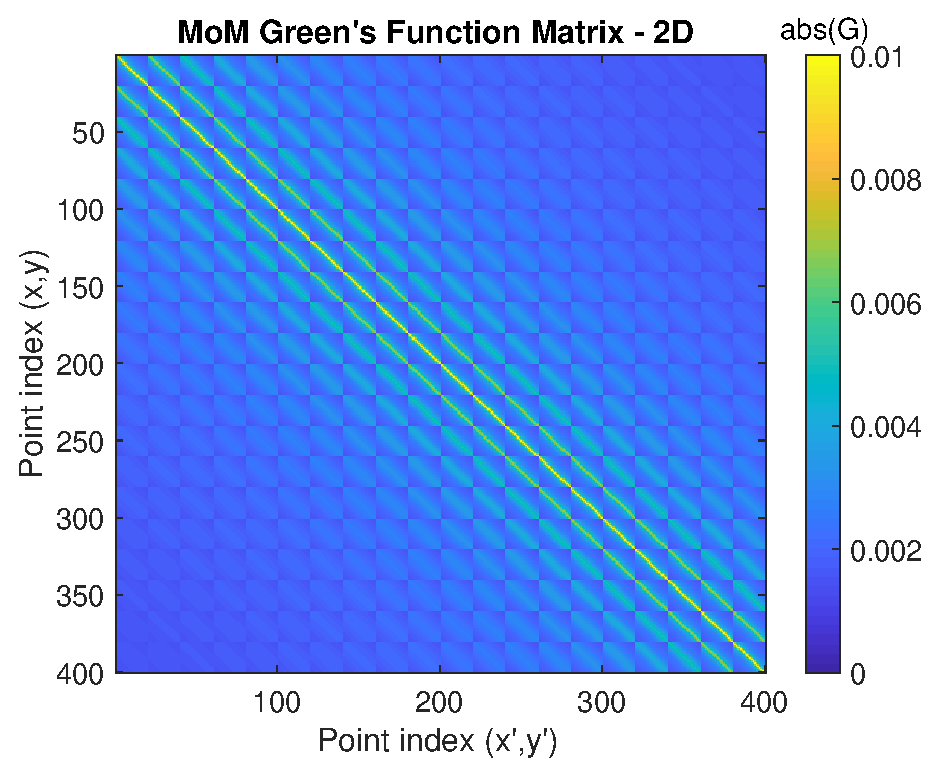
\includegraphics[width=2.5in]{GreensFunctions/Figures/green2d}}
     \subfigure{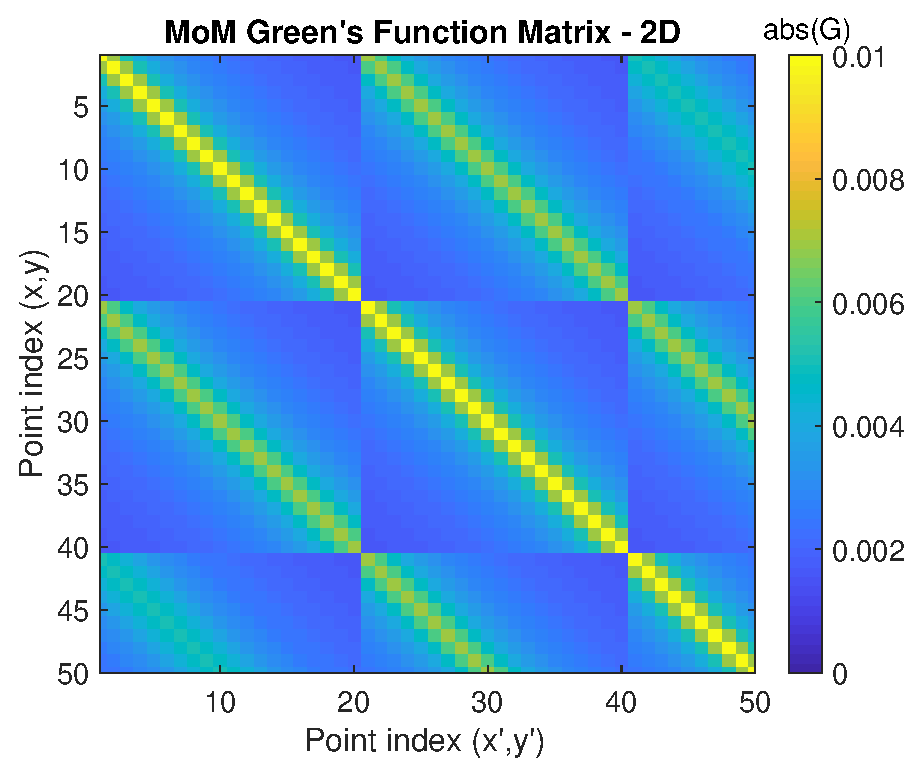
\includegraphics[width=2.5in]{GreensFunctions/Figures/green2d_v2}}
  \end{tabular}
  \label{}
\caption{2D scalar Green's function matrix, $\bb{G}$. Left: absolute value of the elements for the full matrix for a 20 $\times$ 20 grid of points sampled at $\lambda/10$ (total size $2\lambda \times 2 \lambda$). Right: zoom in. The blocks are due to vectorizing the 2D grid of points and then taking all possible pairs of interactions. For example, the upper left 20 $\times$ 20 block contains the $20^2$ interactions between the 20 points along one edge of the 2D grid. The diagonal of the matrix contains the self terms.}
\end{figure}


\begin{figure}[H] 
   \centering
      \begin{tabular}{cc}
     \subfigure{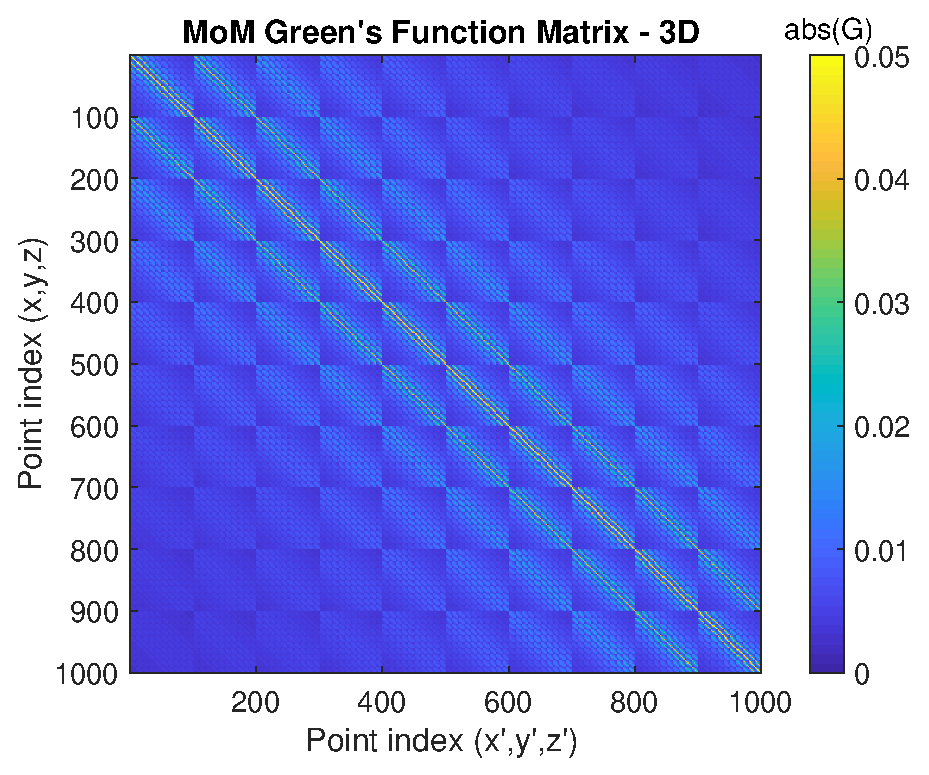
\includegraphics[width=2.5in]{GreensFunctions/Figures/green3d}}
     \subfigure{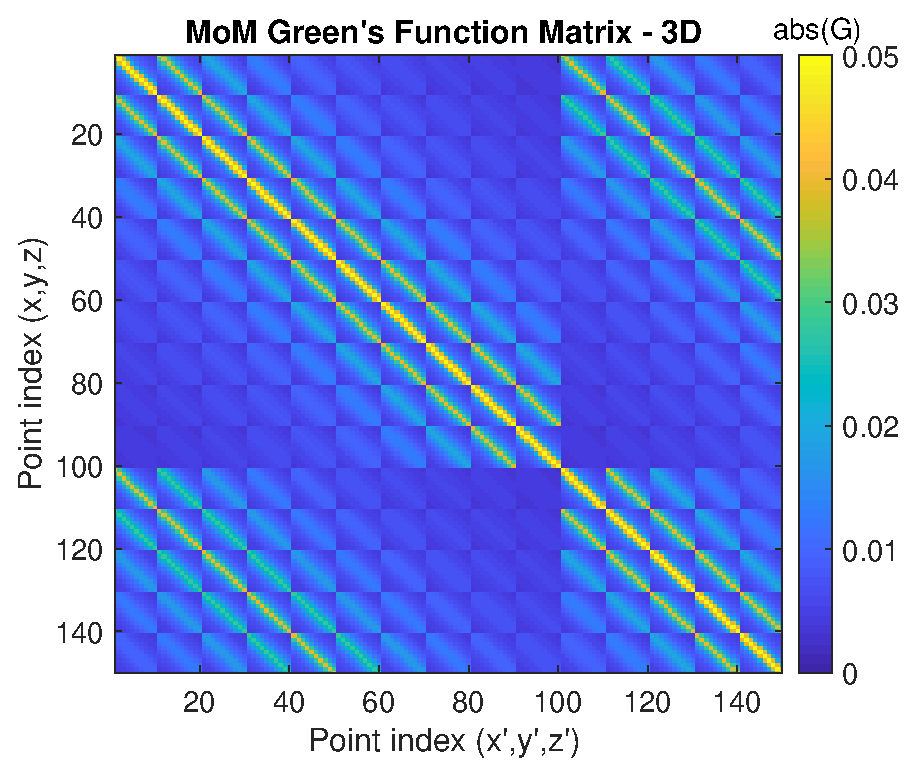
\includegraphics[width=2.5in]{GreensFunctions/Figures/green3d_v2}}
  \end{tabular}
  \label{}
\caption{3D scalar Green's function matrix, $\bb{G}$. Left: full matrix for a 10 $\times$ 10 $\times$ 10 grid of points sampled at $\lambda/5$ (total size of $2\lambda \times 2\lambda \times 2\lambda$). Note, this discretization step is for illustration purposes and is insufficient for an accurate solution. Right: zoom in. The appearance of blocks and subblocks is due to first vectorizing the 3D grid of points, and then taking all possible pairs of interactions which are arranged across rows and columns. For example, the first upper left subblock (sized 10 $\times$ 10), contains the 100 pairs of interactions between the 10 points along one edge of the 3D grid. The diagonal of the matrix are the self terms. }
\end{figure}


\vspace{-5mm}
\paragraph{Routines} The routine \texttt{momGmatrix2D} returns the 2D scalar Green's function matrix for the MoM solution. It takes as input the side length of the square voxel, $\Delta x$, which is assumed constant for all voxels, the background wavenumber $k_b$, and the $(x,y)$ and $(x',y')$ coordinate pairs at which the Green's function will be evaluated. The voxel size length is used to evaluate the volume-integrated singular and non-singular scalar factors which are automatically included in the matrix elements. The arrays of unprimed and primed coordinate pairs can be different sizes: the output matrix is sized $M \times N$ where $M$ is the total number of unprimed points down rows, and $N$ is the total number of primed points across columns. The inputs of primed and unprimed coordinates are separated to facilitate the construction of $\bb{G}$ in subblocks when the number of points is large. If the complete matrix is desired, just input the same arrays for unprimed and primed coordinates, and the routine will return the full square matrix. The points are vectorized column-wise, so the corresponding object function or incident field need to be vectorized column-wise to be consistent. 


{\scriptsize
\VerbatimInput{\code/GreensFunctions/momGmatrix2D.m}
}

\clearpage
The routine \texttt{momGmatrix3D} returns the 3D scalar Green's function matrix for the MoM solution. It takes as input the side length of the cubic voxel, $\Delta x$, which is assumed constant for all voxels, the background wavenumber $k_b$, and the $(x,y,z)$ and $(x',y',z')$ coordinate pairs at which to evaluate the matrix. It otherwise works the same as \texttt{momGmatrix2D}. Because the MoM matrix scales as $O(N^2)$ with the number of 3D voxels, $N$, the total number of elements scales as $O(L^6)$, where $L$ is the side length of a cubic simulation region.



{\footnotesize
\VerbatimInput{\code/GreensFunctions/momGmatrix3D.m}
}



\subsection{Vector MoM}

The vector MoM is derived the same way as the scalar MoM. The major difference is in bookkeeping the vector components and the size of the final matrix. The full vector formulation is needed for any 3D vector scattering problem.  

\paragraph{Total Field}

Starting with the vector VIE, \eqref{vectorVIE}, and substituting the pulse basis function
\eq{\bb{E}(\br) = \bb{E}_{inc}(\br) + \sum_{n}  \int \G{} \cdot O_{n} \delta_{n}(\br') \bb{E}(\br') dV' }

As with the scalar case, the field is assumed constant in each voxel and indexed as
\eq{\bb{E}(\br_m) = \bb{E}_{inc}(\br_m) + \sum_{n}  \int \overline{\bb{G}}(\br_m,\br')  \cdot O_{n} \delta_{n}(\br') \bb{E}(\br_n) dV' }

Assuming Cartesian vector components, $u = (x,y,z)$ and $v = (x,y,z)$, and integrating the dyadic Green's function over the volume-equivalent sphere of the cubic voxel, this is written as a sum for each total field component as
\eq{E_{u,m} = E_{inc,u,m} +  \sum_{v}\sum_{n} G_{uv,mn} O_{n} E_{v,n} \label{Ediscrete} }
\eq{G_{uv,mn} = \begin{cases} G_{uv}(\bb{r}_m,\bb{r}_n) \Delta V, \quad m \neq n\\
G_{uv}(\bb{r}_m=\bb{r}_n), \qquad m = n, u = v \quad (0, u \ne v)  \end{cases}}

\noindent where $\Delta V$ is given by \eqref{voxelint}. The value of the singular integration at the self term, \eqref{singintvec}, is equal to a constant times the identity dyad. The identity dyad means that the self-term only applies to the diagonal elements of the dyad (i.e., $G_{xx}, G_{yy}, G_{zz}$) and is zero for the off-diagonal elements of the dyad. Writing this in matrix notation for the three unknown total field components 
\eq{\left(\bb{I} - \thbth
{\bb{G}_{xx}}{\bb{G}_{xy}}{\bb{G}_{xz}}
{\bb{G}_{yx}}{\bb{G}_{yy}}{\bb{G}_{yz}}
{\bb{G}_{zx}}{\bb{G}_{zy}}{\bb{G}_{zz}} 
\thbth{\bb{O}}{}{}{}{\bb{O}}{}{}{}{\bb{O}}  \right) \thrcol{\bb{E}_x}{\bb{E}_y}{\bb{E}_z} = \thrcol{\bb{E}_{inc,x}}{\bb{E}_{inc,y}}{\bb{E}_{inc,z}} \label{mommatrixtot}}

\noindent where $\bb{I}$ is the identity matrix, $\bb{G}_{uv}$ is the Green's function matrix block for a given polarization pair, $\bb{E}_{inc,v}$ and $\bb{E}_{v}$ are vectors of the incident field and total field solution, respectively, $\bb{O}$ is the diagonal matrix of the object function which is applied to each component. The self term (diagonals) of $\bb{G}_{xx}, \bb{G}_{yy}, \bb{G}_{zz}$, take the value, \eqref{singintvec}, while the self terms of the other blocks are zero. Recall, $\bb{G}_{uv} = \bb{G}_{vu}$, and each block matrix is square symmetric. The size of each block matrix and field vector is the same size as the scalar case. The field components lead to 3 times as many unknowns as compared to the scalar cases, and polarization mixing makes the MoM matrix 9 times larger than the 3D scalar case. 


\paragraph{Induced Current}

Define the induced current as the product of the contrast and the total field at a given point
\eq{ \bb{J}(\br)  =  O(\br) \bb{E}(\br)}

Then \eqref{mommatrixtot} can be written 
\eq{\left(\thbth{\bb{O}^{-1}}{}{}{}{\bb{O}^{-1}}{}{}{}{\bb{O}^{-1}}  - \thbth
{\bb{G}_{xx}}{\bb{G}_{xy}}{\bb{G}_{xz}}
{\bb{G}_{yx}}{\bb{G}_{yy}}{\bb{G}_{yz}}
{\bb{G}_{zx}}{\bb{G}_{zy}}{\bb{G}_{zz}} 
 \right) \thrcol{\bb{J}_x}{\bb{J}_y}{\bb{J}_z} = \thrcol{\bb{E}_{inc,x}}{\bb{E}_{inc,y}}{\bb{E}_{inc,z}}  }


\begin{figure}[H] 
   \centering
      \begin{tabular}{cc}
     \subfigure{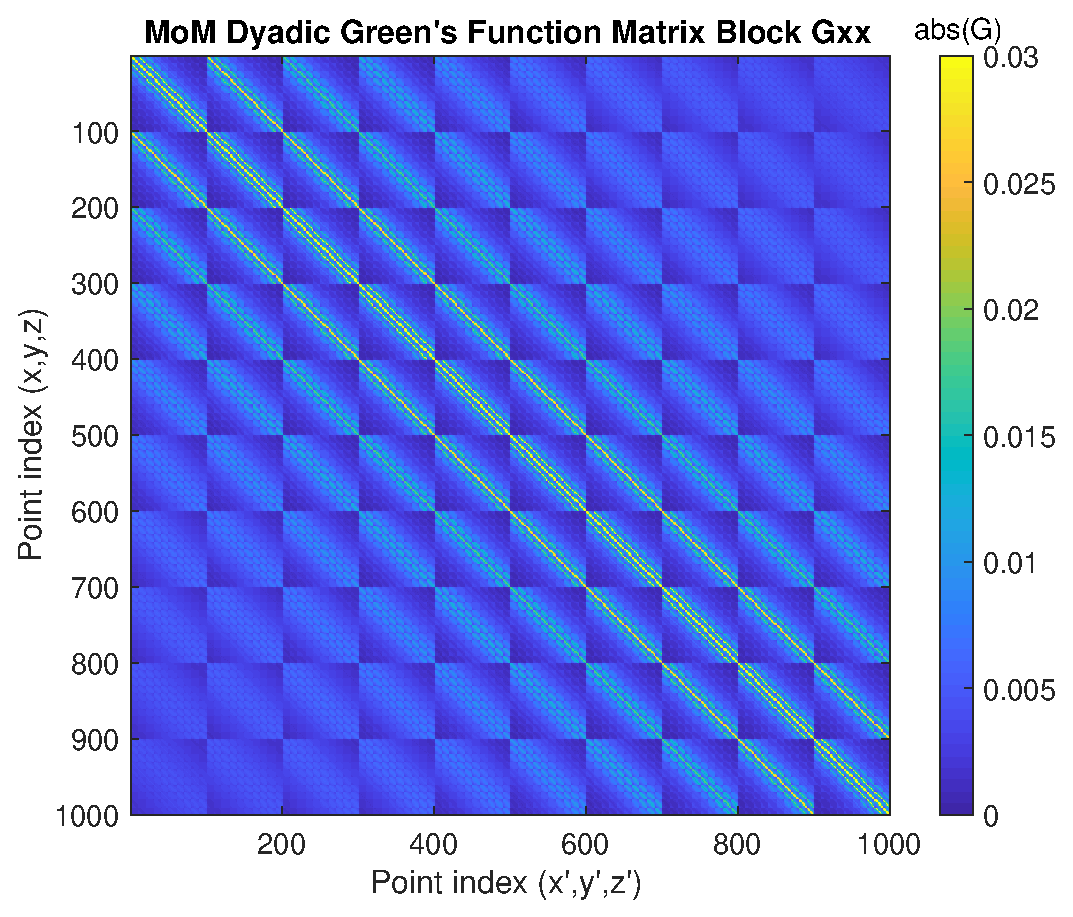
\includegraphics[width=1.9in]{GreensFunctions/Figures/green3dyadic1}}
     \subfigure{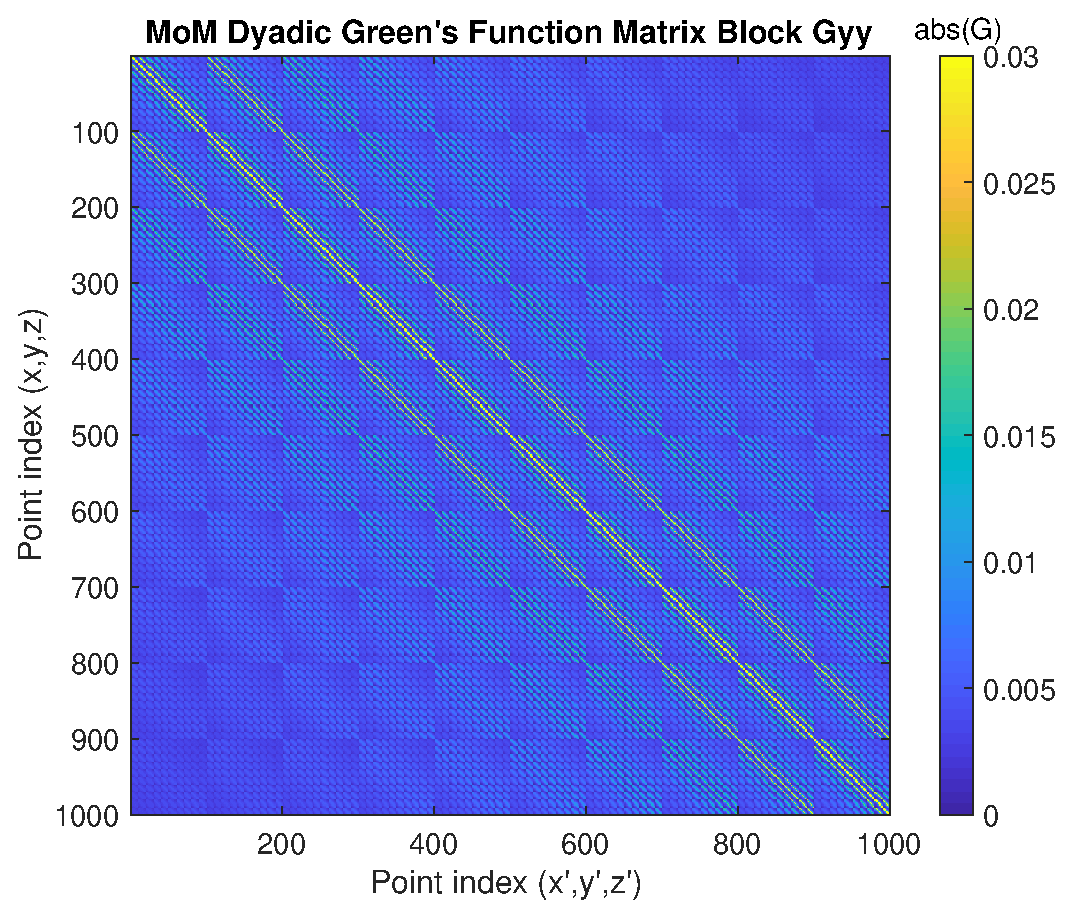
\includegraphics[width=1.9in]{GreensFunctions/Figures/green3dyadic2}} 
     \subfigure{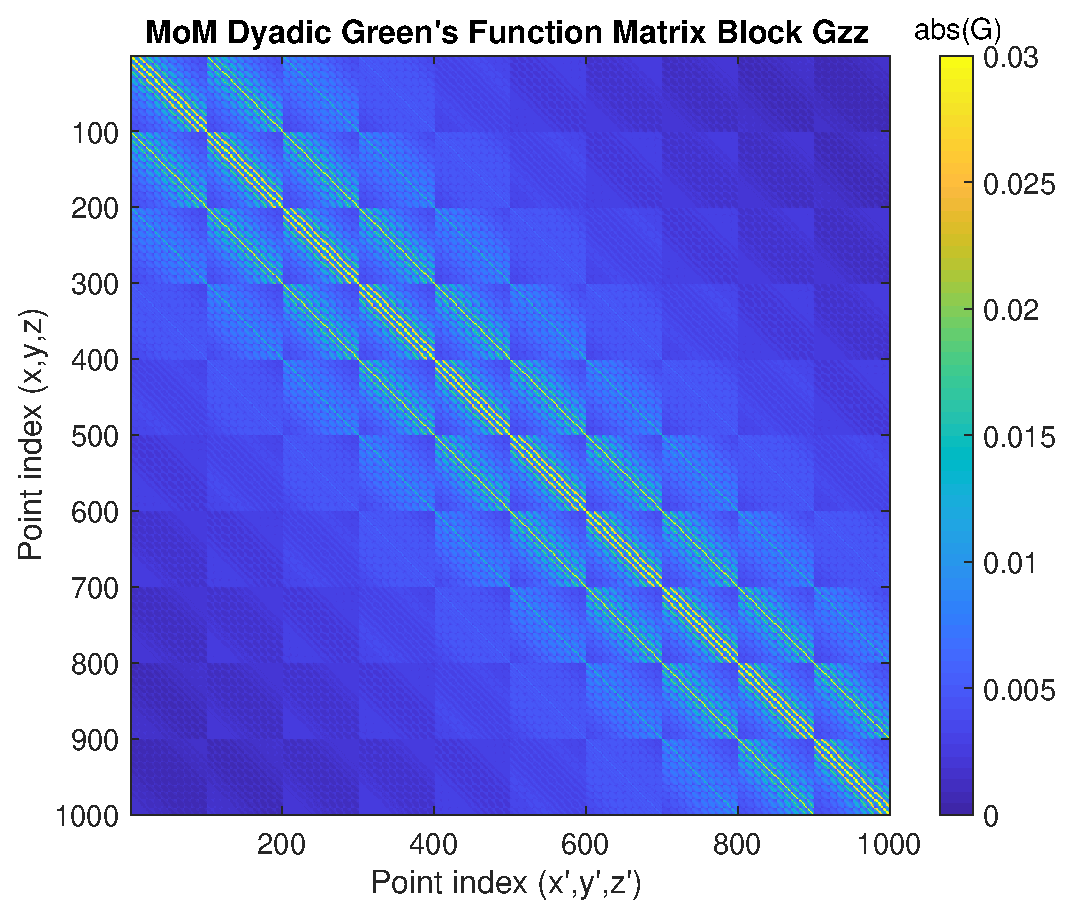
\includegraphics[width=1.9in]{GreensFunctions/Figures/green3dyadic3}} \\
     \subfigure{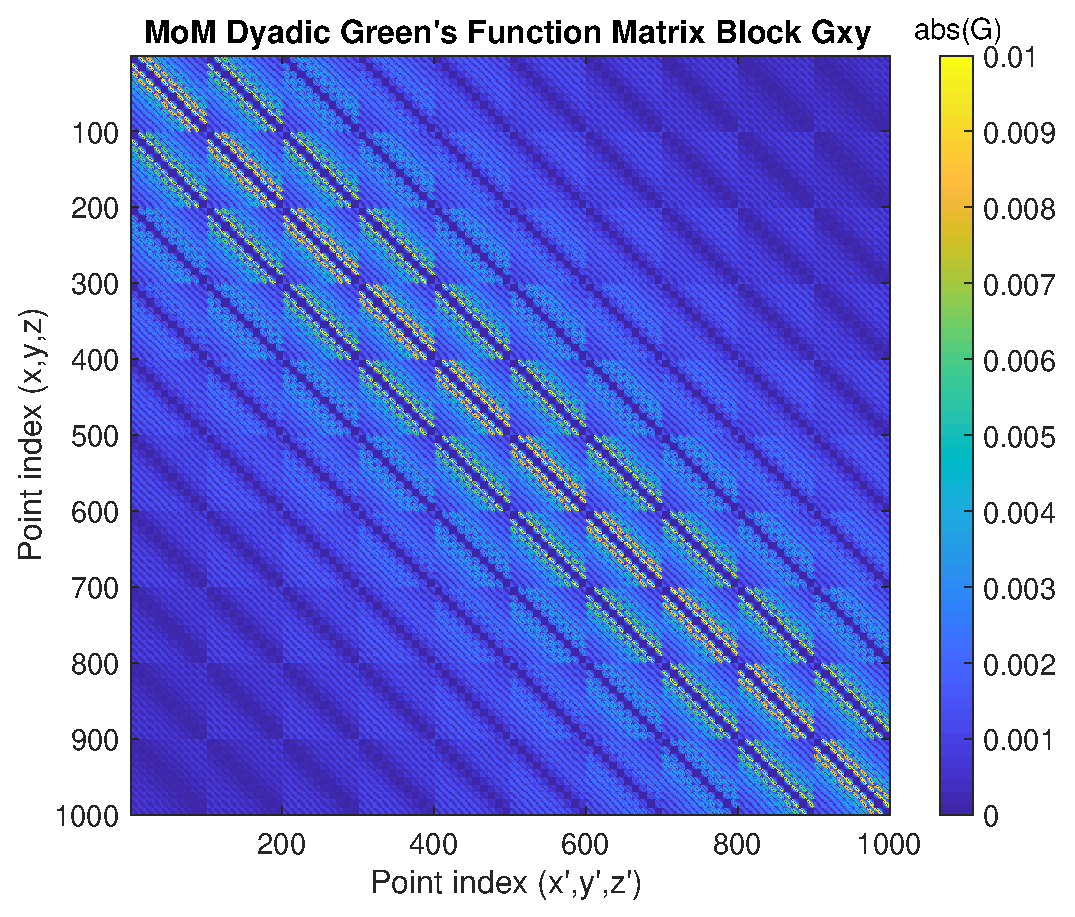
\includegraphics[width=1.9in]{GreensFunctions/Figures/green3dyadic4}} 
     \subfigure{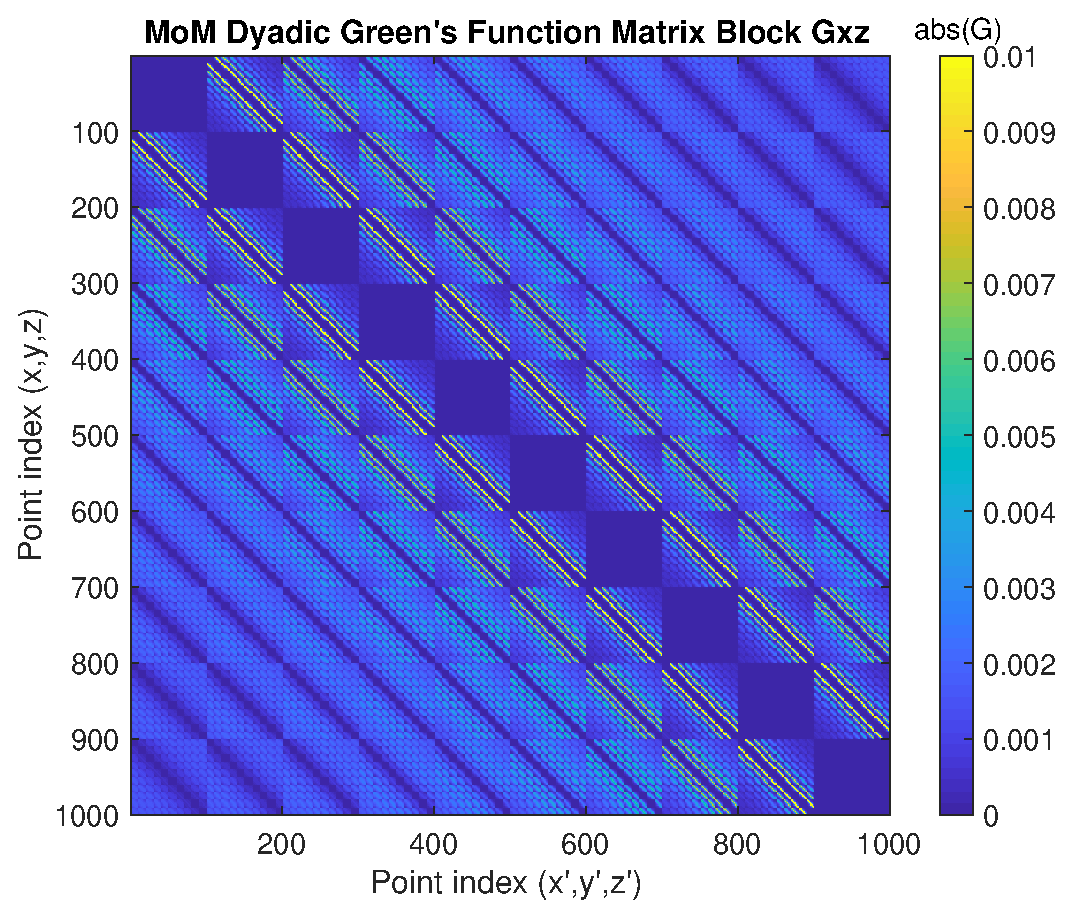
\includegraphics[width=1.9in]{GreensFunctions/Figures/green3dyadic5}}
     \subfigure{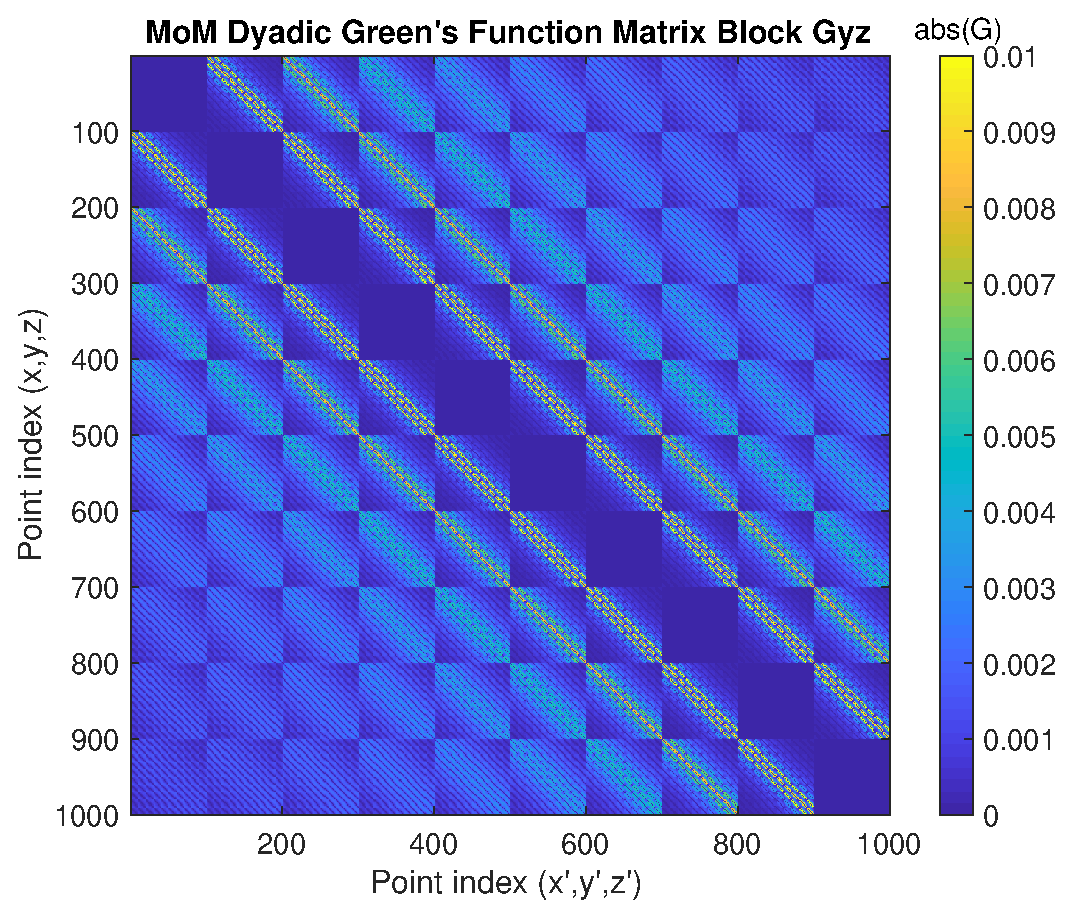
\includegraphics[width=1.9in]{GreensFunctions/Figures/green3dyadic6}}
  \end{tabular}
  \label{}
\caption{3D dyadic Green's function block matrices, $\bb{G}_{uv}$. Full block matrices for a 10 $\times$ 10 $\times$ 10 grid of points sampled at $\lambda/5$ (total size of $2\lambda \times 2\lambda \times 2\lambda$). The zero elements in $\bb{G}_{u \ne v}$ happen when voxels have common coordinates in either $u$ or $v$. This is a result of $\bb{G}_{u \ne v}$ being proportional to the difference of primed and unprimed coordinates in $u$ or $v$. }
\end{figure}

\paragraph{Routine} The routine \texttt{momGmatrixDyadic} returns the 6 unique block matrices of the 3D dyadic MoM matrix.  It takes as input the side length of the cubic voxel, $\Delta x$, which is assumed constant for all voxels, the background wavenumber $k_b$, and the $(x,y,z)$ and $(x',y',z')$ coordinate pairs at which to evaluate the matrix. It works similarly to \texttt{momGmatrix2D} and \texttt{momGmatrix3D}, but calls \texttt{dyadicGreens} which takes the relative positions as input. The arrays of unprimed and primed coordinate pairs can be different sizes. The output matrix is sized $M \times N$ where $M$ is the total number of unprimed points down rows, and $N$ is the total number of primed points across columns. In the routine, the volume integrated constants are applied to all entries. The singularity constant is applied to the self terms of the blocks $\bb{G}_{u = v}$, while the self terms of the blocks $\bb{G}_{u \ne v}$ are set to zero. 



{\footnotesize
\VerbatimInput{\code/GreensFunctions/momGmatrixDyadic.m}
}

\clearpage
\newpage

\section{Scattered Field VIE}

Once the total field solution is found, the scattered field away from the object is computed again with the VIE. Here, the unprimed position vector of the Green's function is evaluated at an observation point outside of the object domain. In this case, the Green's function is often referred to as the receiver Green's function. This can be a point of confusion when comparing it to the Green's function as used in the MoM solution, where the unprimed position vector is evaluated throughout the object domain including at singular points. In the end, the receiver Green's function is the same as the one used in the MoM solution, except that the unprimed position vector is simply evaluated outside of the object at a point that is also usually associated with a sensor.

From reciprocity, it turns out that the receiver Green's function is equivalent to the incident field generated by a point source at the observation location. This is practically and conceptually useful. It links the incident field needed when solving for the total field solution to the scattered field VIE needed to compute the measurements from sources or receivers at the same location. This idea is generalized to the case of real antennas fed by waveguides using the waveport vector Green's function described in \cite{haynes2012vector}. The overarching idea here is that only the incident field of a source or an antenna needs to be known in order to compute both the total field solution and the received voltage measurements in a consistent way. 

\subsection{Receiver Green's Function}
\paragraph{Scalar case}
Let a source be at location $\br_i$. This generates an incident field, $\phi_{inc,i}(\br)$, for which the total field solution in the object is $\phi_{i}(\br)$. The scattered field observed at a point, $\br_j$, outside the object is
\eq{\phi_{sca,ji}(\br_j) = \int g(\br_j,\br') O(\br') \phi_i(\br') dV', \qquad \br_{j} \notin V \label{scalarscaji}}

\noindent where, $g(\br_j,\br')$ is the receiver Green's function. The receiver Green's function is named this way because the unprime variable is evaluated at the receiver, or observation, point. This VIE is discretized the same way as the MoM: the Green's function is integrated over volume-equivalent voxels so that
\eq{\phi_{sca,ji}(\br_j) \approx \Delta V \sum_{n} g(\br_j,\br_n) O(\br_n) \phi_i(\br_n) \label{scalarscadiscrete}}
 
\noindent where $\Delta V$ is given by \eqref{voxelint} in the 3D case. Because $\br_{j} \notin V$, there is no singular point to deal with.

\paragraph{Vector case}

Let a vector source, like an antenna, be located at $\br_i$. This generates an incident field, $\bb{E}_{inc,i}(\br)$, for which the total field solution in the object is $\bb{E}_{i}(\br)$. The scattered field observed at a point, $\br_j$, outside the object is
\eq{\bb{E}_{sca,ji}(\br_j)=  \int \overline{\bb{G}}(\br_j,\br')\cdot O(\br') \bb{E}_i(\br') dV', \qquad \br_{j} \notin V \label{vectorscaji} }

Here, $\overline{\bb{G}}(\br_j,\br')$ is the dyadic receiver Green's function. Discretized like the MoM, this is 
\eq{\bb{E}_{sca,ji}(\br_j) \approx   \Delta V\sum_{n}  \overline{\bb{G}}(\br_j,\br_n)  \cdot O(\br_n) \bb{E}_i(\br_n) \label{vectorscadiscrete} }

\noindent where $\Delta V$ is given by \eqref{voxelint}, there is no singular point, and the dyadic Green's function is evaluated normally. 

\subsection{Incident Field Reciprocity}

The receiver Green's function is equivalent to the incident field generated by a point source at the receiver location when used in transmit mode. This is a consequence of the definition of the Green's function and reciprocity. The derivation is simple, but the idea has important implications for linking the VIE to measurements in experimental setups. In short, the incident field alone fully characterizes the transmit and receive characteristics of a reciprocal sensor. We derive the results for scalar and vector point sources, but the results hold for arbitrary source distributions. 

\paragraph{Scalar case}

Define a scalar point source at location $\br_j$ as $s(\br) = -\delta(\br - \br_j)$. Using \eqref{sourceintscalar}, the incident field from this source is
\ea{\phi_{inc,j}(\br) &=&  -\int g(\br,\br') s(\br') dV' \\
\ &=& \int g(\br,\br') \delta(\br' - \br_j) dV' \\
\ &=&  g(\br,\br_j) }

This is another way of stating the definition of the Green's function. Using the fact that $g(\br,\br_j) = g(\br_j,\br)$, and substituting this into \eqref{scalarscaji}, the scattered field VIE is
\eq{\phi_{sca,ji}(\br_j) = \int \phi_{inc,j}(\br') O(\br') \phi_i(\br') dV' \label{scalarscajiinc}}

The incident field from the point source takes the place of the receiver Green's function. From linearity, this holds for an incident field from an arbitrary source distribution so long as the same device is used as the receiver. Finally, \eqref{scalarscajiinc} is discretized the same as \eqref{scalarscadiscrete}. 

\paragraph{Vector case}

Let the current source be an infinitesimal dipole at $\br_j$ with strength $I$ and polarization $\hat{\bb{p}}$
\eq{\bb{J}(\br) = I \hat{\bb{p}} \delta(\br - \br_j)}

Substituting this into \eqref{evolintj}
\ea{\bb{E}_{inc,j}(\br) &=& i\omega\mu\int \overline{\bb{G}}(\br,\br') \cdot \bb{J}(\br') dV' \\
 \ &=& i\omega\mu I \int \overline{\bb{G}}(\br,\br') \cdot \hat{\bb{p}} \delta(\br' - \br_j) dV'  \\
  \ &=& i\omega\mu I  \overline{\bb{G}}(\br,\br_j) \cdot \hat{\bb{p}} }

or
\ea{ \overline{\bb{G}}(\br,\br_j) \cdot \hat{\bb{p}} = \dfrac{1}{i\omega\mu I }\bb{E}_{inc,j}(\br)  }

A similar expression can be found in \cite{cui2004study} for 2D problems. The columns of the dyadic receiver Green's function are found by computing the incident field due to three orthogonal dipoles in turn. Denote these incident fields $\bb{E}_{inc,j,p}$ for dipole polarizations $p = [x, y, z]$ located at the observation point. Then using the fact that $\overline{\bb{G}}(\br,\br_j) = \left[ \overline{\bb{G}}(\br_j,\br)\right]^{t}$, we have
\eq{ \overline{\bb{G}}(\br_j,\br)  = \dfrac{1}{i\omega\mu I }\cvec{\bb{E}_{inc,j,x}^t(\br)}{\bb{E}_{inc,j,y}^t(\br)}{\bb{E}_{inc,j,z}^t(\br)} \label{incdyad}}

The matrix on the right hand side is denoted the incident field dyad. The transposes place the $[x,y,z]$ vector components of each dipole incident field along the rows of the dyad, which maps the three-vector total field (or induced source) in the domain to the polarizations of the source dipole at the receiver location. Substituting this into \eqref{vectorscaji}, the scattered field VIE for the electric field is
\eq{\bb{E}_{sca,ji}(\br_j)= \dfrac{1}{i\omega\mu I }\int \cvec{\bb{E}_{inc,j,x}^t(\br')}{\bb{E}_{inc,j,y}^t(\br')}{\bb{E}_{inc,j,z}^t(\br')} \cdot O(\br') \bb{E}_i(\br') dV' \label{vectorscajiinc} }

In simulation, one can set $I = 1/i\omega\mu$ to cancel the scale factor and \eqref{vectorscajiinc} can be discretized like \eqref{vectorscadiscrete}. The physical interpretation of \eqref{vectorscajiinc} is the following. The three source dipoles at the observation location independently map to a three-vector incident field in the object domain. Concurrently, each vector component of the induced current in the domain radiates all three vector components to the observation point. The columns of the incident field dyad, \eqref{incdyad}, map any single component of the induced current to the three components at the observation location in proportion to the strength of the incident fields created by the corresponding source dipoles. This is another way of stating reciprocity. %For example, an $x$ directed current in the object radiates all three vector components at the observation point and the weights of this mapping are determined are determined by the $x$ components of each of the three incident fields. The same happens for the other two components to accomplish the full dyadic mixing. 


\subsection{Waveport Vector Green's Function}
When measuring fields with real antennas, we never measure the three electric field components directly. We measure a voltage on a feeding waveguide or transmission line. The three vector components of the scattered field are effectively integrated over the surface of the antenna and produce the voltage on the waveguide. The incident field dyad above collapses to three-vector incident field with certain scale factors. This was formalized in \cite{haynes2012vector} in the form a waveport vector Green's function. The idea is fundamentally the same as the receiver Green's function and incident field dyad, except that it is specialized for S-parameter measurements between two antennas that are made using a vector network analyzer (VNA) with calibrated reference planes on the feeding transmission lines. 

\begin{figure}[H] 
\centering
\includegraphics[width=3in]{GreensFunctions/Figures/SparamVIE}
\caption{Network model of two antennas and a scattering object. $S$-parameters are measured between the reference planes on antenna transmission lines, \cite{haynes2012vector}.}
\label{sparamviefig}
\end{figure}

Let two antennas in frames $i$ and $j$ be used to probe an object with a VNA that measures the entire system as a 2-port device, as shown in Figure \ref{sparamviefig}. The complex excitation amplitudes on each transmission line are $a_o^i$ and $a_o^j$, while the received amplitudes are $b_o^i$ and $b_o^j$. The VNA is calibrated to the reference planes on the transmission lines. Assume that the spatial distribution of the antenna incident field is referenced to a fixed coordinate origin of the antenna, and the excitation (amplitude and phase) is referenced to the calibration planes on the transmission line. The waveport vector Green's function is
\eq{\bb{g}(\br) = -\dfrac{Z_o}{2a_o}\dfrac{1}{i\omega\mu} \bb{E}_{inc}(\br)}

\noindent where $Z_o$ is the characteristic impedance of the receiver transmission line and $a_o$ is the excitation used to create the incident field $\bb{E}_{inc}(\br)$. The waveport vector Green's replaces the dyadic receiver Green's function \eqref{incdyad} and effectively collapses the dyad.
When used in the VIE, the 2-port scattered field $S$-parameter measurement, $S_{ji}$, is given by 
\eq{S_{ji} = -\dfrac{1}{2i\omega\mu} \dfrac{Z_o^j}{a_o^j a_o^i} \int \bb{E}_{inc,j}(\br') \cdot O(\br') \bb{E}_{i}(\br') dV'}

\noindent where $a_o^j$ is the excitation used to create the incident field of the receiver, $\bb{E}_{inc,j}(\br')$, and $a_o^i$ is the excitation used to create the incident field of the transmitter $\bb{E}_{inc,i}(\br')$ which in turn is used to compute the solution of the total field $\bb{E}_{i}(\br')$.  In practice, if we know the average transmit power on the transmission line, $P_{ave}$, then from transmission line analysis the magnitude of $a_o$ is given by 
\eq{\vert a_o \vert = \sqrt{2 Z_o P_{ave}}}

The phase of $a_o$ can be found by comparing the transmission line reference plane used to measure or simulate the incident fields to the reference planes used in measurement. 











\chapter{Spherical Wave Functions}
\label{chap:wavefunctions}


This chapter gives routines and tools for computing and using scalar and vector wave functions in free-space spherical coordinates. The wave functions represent the frequency-domain multipoles of the field, which together give the multipole expansion of a field. While the wave functions themselves are not always used, the coefficients of the expansions are quite useful. The expansion coefficients can be quickly manipulated by rotation and translation addition theorems to transform the fields in different reference frames (see Chapters \ref{chap:rotation} and \ref{chap:translation}). This chapter provides codes for spherical wave functions and serves as a quick reference for certain properties and derivations. 

\section{Indexing}

Spherical harmonics and spherical wave functions are defined by the degree and order of the underlying associated Legendre polynomials, $(l,m)$. It is convenient to store and access harmonics using a linear index. For vector wave functions, where the harmonics range from $l = 1,...,L$ and $m = \pm l$, the linear index for harmonic $(l,m)$ is given by $n = l^2 + l + m$. When the set of harmonics includes all $m$ at each $l$, the total number of harmonics is $N = L^2 + 2L$. The following sequence converts a linear index $n$ to $(l,m)$ for vector wave functions:
\begin{eqnarray}
l &=& \lfloor \sqrt{n} \rfloor \\
m &=& n - l^2 - l
\end{eqnarray}

Table \ref{linearindexvec} illustrates the mapping between linear index and harmonic for vector waves. A similar table appears in \cite{tsang2000scattering}.  Scalar wave functions include degree $l=0$, which is the monopole. The linear index is then given by $n = l^2 + l + m + 1$.  When the set of harmonics includes all $m$ at each $l$, the total number of harmonics is $N = L^2 + 2L + 1$.  The following sequence converts a linear index $n$ to $(l,m)$ for scalar waves:
\begin{eqnarray}
l &=& \lfloor \sqrt{n-1} \rfloor \\
m &=& n - l^2 - l -1
\end{eqnarray}

Table \ref{linearindexmono} illustrates the mapping for scalar wave functions including the monopole.  


The function \texttt{lm2ind} returns the linear index for pair $(l,m)$, while \texttt{ind2lm} outputs the $(l,m)$ pair given the index.   Use the string switch \texttt{'mono'} to include the monopole for scalar waves. \texttt{lmtable} produces a table of $(l,m)$ pairs. These routines are useful for general purpose manipulation of spherical harmonic indexing or when developing routines. However, the error checking slows them down and should be replaced by inline expressions once routines are debugged.  



\begin{table}[H]
\parbox{.45\linewidth}{
\caption{Vector Wave Function Harmonic Indexing}
\centering
\begin{tabular}{|c|c|c|}
\hline
Linear index & $l$ & $m$ \\
\hline
1 &      1  &  -1 \\
2 &      1  &   0\\
3 &      1  &   1\\
\hline
4 &      2  &  -2\\
5 &      2   & -1\\
6 &      2   &  0\\
7 &      2   &  1\\
8 &      2   &  2\\
\hline
9 &      3   & -3\\
10 &      3  &  -2\\
11 &      3  &  -1\\
12 &      3  &   0\\
13 &      3   &  1\\
14 &      3   &  2\\
15 &      3  &   3 \\
\hline
\end{tabular}
\label{linearindexvec}
}
\hfill
\parbox{.45\linewidth}{
\centering
\caption{Scalar Wave Function Harmonic Indexing}
\centering
\begin{tabular}{|c|c|c|}
\hline
Linear index & $l$ & $m$ \\
\hline
1 & 	0 & 0 \\
\hline
2 &      1  &  -1 \\
3 &      1  &   0\\
4 &      1  &   1\\
\hline
5 &      2  &  -2\\
6 &      2   & -1\\
7 &      2   &  0\\
8 &      2   &  1\\
9 &      2   &  2\\
\hline
10 &      3   & -3\\
11 &      3  &  -2\\
12 &      3  &  -1\\
13 &      3  &   0\\
14 &      3   &  1\\
15 &      3   &  2\\
16 &      3  &   3 \\
\hline
\end{tabular}
%\caption{Scalar Wave Function Harmonic Indexing}
\label{linearindexmono}
}
\end{table}


%
%\begin{table}[htp]
%\caption{Vector Wave Function Harmonic Indexing}
%\begin{center}
%\begin{tabular}{|c|c|c|}
%\hline
%Linear index & $l$ & $m$ \\
%\hline
%1 &      1  &  -1 \\
%2 &      1  &   0\\
%3 &      1  &   1\\
%\hline
%4 &      2  &  -2\\
%5 &      2   & -1\\
%6 &      2   &  0\\
%7 &      2   &  1\\
%8 &      2   &  2\\
%\hline
%9 &      3   & -3\\
%10 &      3  &  -2\\
%11 &      3  &  -1\\
%12 &      3  &   0\\
%13 &      3   &  1\\
%14 &      3   &  2\\
%15 &      3  &   3 \\
%\hline
%\end{tabular}
%\end{center}
%\label{linearindexvec}
%\end{table}




%
%\begin{table}[htbp]
%\caption{Scalar Wave Function Harmonic Indexing}
%\begin{center}
%\begin{tabular}{|c|c|c|}
%\hline
%Linear index & $l$ & $m$ \\
%\hline
%1 & 	0 & 0 \\
%\hline
%2 &      1  &  -1 \\
%3 &      1  &   0\\
%4 &      1  &   1\\
%\hline
%5 &      2  &  -2\\
%6 &      2   & -1\\
%7 &      2   &  0\\
%8 &      2   &  1\\
%9 &      2   &  2\\
%\hline
%10 &      3   & -3\\
%11 &      3  &  -2\\
%12 &      3  &  -1\\
%13 &      3  &   0\\
%14 &      3   &  1\\
%15 &      3   &  2\\
%16 &      3  &   3 \\
%\hline
%\end{tabular}
%\end{center}
%\label{linearindexmono}
%\end{table}

{\footnotesize
\VerbatimInput{\code/Wavefunctions/lm2ind.m}
}
{\footnotesize
\VerbatimInput{\code/Wavefunctions/ind2lm.m}
}

{\footnotesize
\VerbatimInput{\code/Wavefunctions/lmtable.m}
}


\clearpage
\section{Spherical Harmonics}

\subsection{$Y_{lm}(\theta,\phi)$}
The fully normalized spherical harmonics are given by
\begin{equation}
Y_{lm}(\theta,\phi) = \sqrt{\dfrac{2l+1}{4\pi}\dfrac{(l-m)!}{(l+m)!}}P_l^m(\cos\theta)e^{im\phi}
\end{equation}

\noindent where $P_l^m(\cos\theta)$ are the associated Legendre polynomials. The Condon-Shortley phase, $(-1)^m$, is included in the definition of $P_l^m(\cos\theta)$. The spherical harmonics can be written in terms of the fully normalized associated Legendre polynomials, $\widetilde P_l^m(\cos\theta)$, as 
\begin{equation}
Y_{lm}(\theta,\phi) = \dfrac{1}{\sqrt{2\pi}} \widetilde P_l^m(\cos\theta) e^{im\phi}
\end{equation}  

Any scalar spherical function can be expanded as a sum of spherical harmonics
\eq{f(\theta,\phi) = \sum_{l=0}^{\infty} \sum_{m=-l}^{l} a_{lm} Y_{lm}(\theta,\phi)}

Being fully normalized, the orthogonality relation for the spherical harmonics is simply
\begin{equation}
\int_0^{2\pi} \int_0^{\pi}Y_{lm}(\theta,\phi) Y^*_{l'm'}(\theta,\phi) \sin\theta d\theta d\phi = \delta_{ll'}\delta_{mm'}
\end{equation}

\noindent where one can show with \eqref{eq2} that
\begin{equation}
Y^*_{lm}(\theta,\phi) = (-1)^mY_{l,-m}(\theta,\phi) 
\label{eq1}
\end{equation}

It is useful to note that 
\eq{\int_0^{2\pi} \int_0^{\pi}Y_{lm}(\theta,\phi) \sin\theta d\theta d\phi =  \sqrt{4 \pi} \delta_{l0}\delta_{m0} }

and 
\eq{Y_{l,0}(0,0) = \sqrt{\dfrac{2l+1}{4\pi}} \label{ylzerozz} }

Fully normalized spherical harmonics are given by the routine \texttt{sphericalY}.  The routine returns the values at points $(\theta,\phi)$ up to degree $L$ for all $\pm m$, linearly indexed.  All the harmonics are returned because it is fastest to compute Legendre polynomials recursively and because field expansions often need all the harmonics. The output is a 2D array with first dimension with the points $(\theta,\phi)$ and second dimension with harmonics size $L^2 + 2L$. This is to facilitate matrix-vector multiplication of the harmonics with a column vector of expansion coefficients. After such multiplication, the result has to be reshaped to the size of the input arrays. Use the string switch \texttt{'mono'} to include the monopole term, in which case the second dimension will be size $L^2 + 2L + 1$.  A naive computation of $Y_{lm}$ would compute and divide the factorials directly.  This is only accurate to about $L=21$.  It is best to use the fully normalized Legendre polynomials, then only a factor of $1/\sqrt{2\pi}$ is needed to complete the normalization.  Finally, this routine does not take advantage of the separability of $\theta$ and $\phi$ in the computation if, for example, the arrays contain redundant points on evenly spaced grids over the sphere.

{\footnotesize
\VerbatimInput{\code/Wavefunctions/sphericalY.m}
}


\subsection{Angular Momentum Operators}

The angular momentum operators, $\mathcal{L}$, for spherical harmonics are quite useful and will be used later to express vector spherical harmonics in Cartesian components. Several properties are repeated here from \cite{angularmomop}, which can also be found in textbooks (the operators are usually denoted with $L$, rather than $\mathcal{L}$). 
\eq{\mathcal{L}^2 Y_{lm} = l(l+1)Y_{lm}}
\eq{\mathcal{L}^2 = \mathcal{L}_x^2 + \mathcal{L}_y^2 + \mathcal{L}_z^2}

\noindent where 
\ea{\bb{\mathcal{L}} &=& -i \bb{r} \times \nabla \\
\ &=& \mathcal{L}_x \hat{x} + \mathcal{L}_y \hat{y} + \mathcal{L}_z \hat{z}}

\noindent where $\mathcal{L}_x$, $\mathcal{L}_y$, and $\mathcal{L}_z$ are differential operators that act on Cartesian vector fields.  The components are combined to create raising and lowering operators:
\ea{\mathcal{L}_{+} &=& \mathcal{L}_x + i \mathcal{L}_y = e^{i\phi}\left(\dd{}{\theta} + i \cot\theta \dd{}{\phi}\right) \\
\mathcal{L}_{-} &=& \mathcal{L}_x - i \mathcal{L}_y = e^{-i\phi}\left(-\dd{}{\theta} + i \cot\theta \dd{}{\phi}\right) \\
\mathcal{L}_{z}  &=& -i\dd{}{\phi} 
}

Adding and subtracting the raising and lower operators give 
\ea{\mathcal{L}_x &=& \dfrac{1}{2}\left(\mathcal{L}_{+} + \mathcal{L}_{-}\right) \\
\mathcal{L}_y &=& \dfrac{1}{2 i}  \left(\mathcal{L}_{+} - \mathcal{L}_{-}\right) }

The operators have the property that 
\ea{\mathcal{L}_{+} Y_{lm} &=& \sqrt{(l-m)(l+m+1)} Y_{l,m+1} \\
\mathcal{L}_{-} Y_{lm} &=& \sqrt{(l+m)(l-m+1)}  Y_{l,m-1} \\
\mathcal{L}_{z} Y_{lm} &=& m Y_{l,m} }


\section{Scalar Spherical Wave Functions}

The spherical scalar wave functions are solutions to the Helmholtz wave equation in free space in spherical coordinates. They are a product of spherical Bessel functions and spherical harmonics.  The form of the Bessel function determines whether the wave is incoming or outgoing, specifically whether the field is regular at the origin or radiating, though they are all standing waves:  
\begin{eqnarray}
\textrm{Incoming regular wave:} \quad \quad\textit{Rg} \psi_{lm}(k,\bb{r}) &=& j_l(kr) Y_{lm}(\theta,\phi) \\
\textrm{Outgoing radiating wave:} \quad  \quad \quad \psi_{lm}(k,\bb{r}) &=& h_l^{(1)}(kr) Y_{lm}(\theta,\phi) 
\end{eqnarray}

\noindent where $j_l(kr)$ and $h_l^{(1)}(kr)$ are spherical Bessel and Hankel functions, respectively, $k$ is the background wavenumber, and \textit{Rg} means being regular (non-singular) at the origin which uses $j_l(kr)$. The wave functions form a complete set, so any scalar field can be expanded as an infinite sum: 
\begin{eqnarray}
\textrm{Incoming regular field:} \quad \quad \phi(\bb{r}) &=& \sum_{l=0}^{\infty} \sum_{m=-l}^l a_{lm} \textit{Rg} \psi_{lm}(k,\bb{r})  \\
\textrm{Outgoing radiating field:} \quad \quad \phi(\bb{r}) &=& \sum_{l=0}^{\infty} \sum_{m=-l}^l b_{lm} \psi_{lm}(k,\bb{r}) 
\end{eqnarray}

The far-field scalar wave functions for radiating waves are found by taking the large argument limit of the Hankel function
\eq{\lim_{kr \rightarrow \infty}  \psi_{lm}(k,\bb{r}) = \dfrac{e^{ikr}}{kr} i^{-l-1} Y_{lm}(\theta,\phi)  }

The addition theorem for the scalar Green's function is given in terms of regular and radiating waves as, \cite{chew1995waves},
\eq{g(\bb{r},\bb{r}') = i k\sum_{l=0}^{\infty} \sum_{m=-l}^l \textit{Rg} \psi_{lm}(k,\bb{r}_{<}) \psi_{lm}(k,\bb{r}_{>}) \label{scalargreens}}

\noindent where $\bb{r}_{<}$ is for the smaller of $\vert \bb{r} \vert$ and $\vert \bb{r}'\vert $ and $\bb{r}_{>}$ is for the greater of $\vert \bb{r}\vert$ and $\vert \bb{r}'\vert$.


The routine \texttt{psilm} returns $\psi_{lm}(k,\br)$ at points $(r,\theta,\phi)$ up to maximum degree $L$, for all $\pm m$, linearly indexed.  $k$ is real or complex.  Like \texttt{sphericalY}, the first dimension has evaluation points and second dimension is size $L^2 + 2L+1$.  Use the string switch \texttt{'rg'} for $\textit{Rg} \psi_{lm}(k,\bb{r})$. Evaluation of the sum over harmonics for all points can be accomplished with matrix-vector multiplication then reshaping the result to match the dimensions of the input coordinates.

{\footnotesize
\VerbatimInput{\code/Wavefunctions/psilm.m}
}

\section{Scalar Plane Wave Expansion}

The expansion of scalar plane waves in terms of spherical waves at the origin is, \cite{tsang2000scattering},
\eq{e^{i \bb{k} \cdot \bb{r}} = 4\pi \sum_{l = 0}^{\infty} \sum_{m = -l}^l i^l  j_l(kr) Y_{lm}(\theta,\phi) Y_{lm}^*(\theta_k,\phi_k) \label{scalarplanewaveexp} }

\noindent where the spherical harmonics are fully-normalized with Condon-Shortley phase and 
\ea{\bb{r} &=& x \hat{x} + y \hat{y} + z \hat{z} \\
\bb{k} &=& k \hat{k} \\
\hat{k} &=& \sin\theta_k \cos\phi_k \hat{x} +  \sin\theta_k\sin\phi_k \hat{y} + \cos\theta_k \hat{z} }

The plane wave expansion coefficients are found by separating the regular scalar wave functions from \eqref{scalarplanewaveexp} and collecting the remaining terms as expansion coefficients as
\ea{e^{i \bb{k} \cdot \bb{r}} &=& \sum_{l = 0}^{\infty} \sum_{m = -l}^l a_{lm} \textit{Rg} \psi_{lm}(k,\bb{r}) \\
a_{lm} &=&  4\pi i^l Y_{lm}^*(\theta_k,\phi_k)}

The routine \texttt{scalarPlaneWaveCoef} routine takes as input the maximum harmonic degree $L$, and the spherical coordinates of the plane wave propagation direction, $(\theta_k, \phi_k)$, and returns the $a_{lm}$ scalar plane wave expansion coefficients for $l = 0,...,L$, for all $\pm m$, linearly indexed. 


{\footnotesize
\VerbatimInput{\code/Wavefunctions/scalarPlaneWaveCoef.m}
}

\clearpage

\section{Vector Spherical Harmonics}
\label{sec:vecsphharm}
Vector spherical harmonics capture the angular variation of a vector field in spherical coordinates and are used for far-field radiation patterns. Their close cousin is the radially independent vector wave function usually notated $\bb{X}_{lm}$, \cite{jackson1999classical}. The three fully normalized vector spherical harmonics, which form an orthonormal basis, are given by, \cite{chew1995waves, tsang2000scattering}, 
\begin{eqnarray}
\bb{P}_{lm}(\theta,\phi) &=& \hat{r}Y_{lm}(\theta,\phi) \\
\  & \ & \nonumber \\
\bb{B}_{lm}(\theta,\phi) &=&\dfrac{1}{\sqrt{ l(l+1)}} r\nabla Y_{lm}(\theta,\phi)  \\
\ &=& N_{lm} \left[\hat\theta \dfrac{d}{d\theta} P_l^m(\cos\theta) + \hat\phi \dfrac{im}{\sin\theta}P_l^m(\cos\theta) \right] e^{im\phi}   \\
\ &=& \dfrac{1}{\sqrt{2\pi l(l+1)}} \left[\hat\theta \dfrac{d}{d\theta} \widetilde{P}_l^m(\cos\theta) + \hat\phi \dfrac{im}{\sin\theta}\widetilde{P}_l^m(\cos\theta) \right] e^{im\phi}  \\
\bb{C}_{lm}(\theta,\phi) &=& \dfrac{1}{\sqrt{ l(l+1)}} \nabla \times \left[ \br Y_{lm}(\theta,\phi) \right] \\
\ &=& N_{lm} \left[\hat\theta \dfrac{im}{\sin\theta}P_l^m(\cos\theta) - \hat\phi \dfrac{d}{d\theta} P_l^m(\cos\theta)  \right] e^{im\phi}  \\
\ &=& \dfrac{1}{\sqrt{2\pi l(l+1)}}  \left[\hat\theta \dfrac{im}{\sin\theta}\widetilde{P}_l^m(\cos\theta) - \hat\phi \dfrac{d}{d\theta} \widetilde{P}_l^m(\cos\theta)  \right] e^{im\phi} 
\end{eqnarray}

\noindent where
\begin{equation}
N_{lm} = \dfrac{1}{\sqrt{l(l+1)}}\sqrt{\dfrac{2l+1}{4\pi}\dfrac{(l-m)!}{(l+m)!}}
\end{equation}

The Condon-Shortley phase, $(-1)^m$, is included in the definition of the associated Legendre polynomials. The following relation exists between $\bb{B}_{lm}$ and $\bb{C}_{lm}$:
\begin{eqnarray}
\bb{B}_{lm}(\theta,\phi) &=& \hat{r} \times \bb{C}_{lm}(\theta,\phi) \\
\bb{C}_{lm}(\theta,\phi) &=& -\hat{r} \times \bb{B}_{lm}(\theta,\phi) 
\end{eqnarray}

In other words, $\bb{B}_{lm}\cdot \hat{\theta} = -\bb{C}_{lm} \cdot\hat{\phi} $ and  $\bb{B}_{lm}\cdot \hat{\phi} = -\bb{C}_{lm} \cdot\hat{\theta} $.  The fully normalized vector spherical harmonics have orthonormality 
\begin{equation}
\int_0^{2\pi} \int_0^{\pi}
\left\{
\begin{array}{c}
\bb{P}_{lm}(\theta,\phi) \cdot \bb{P}^*_{lm}(\theta,\phi) \\
\bb{B}_{lm}(\theta,\phi) \cdot \bb{B}^*_{lm}(\theta,\phi) \\
\bb{C}_{lm}(\theta,\phi) \cdot \bb{C}^*_{lm}(\theta,\phi) 
\end{array}
\right\}
\sin\theta d\theta d\phi = \delta_{ll'}\delta_{mm'}
\end{equation}

and
\eq{\int_0^{2\pi} \int_0^{\pi}\bb{B}_{lm}(\theta,\phi) \cdot \bb{C}^*_{lm}(\theta,\phi) \sin\theta d\theta d\phi= 0}

Any spherical vector field (i.e., polarized spherical far-field pattern) can be expanded as
\begin{equation}
\bb{F}(\theta,\phi) = \sum_{l=1}^{\infty}\sum_{m=-l}^l b_{lm} \bb{B}_{lm}(\theta,\phi) + c_{lm}\bb{C}_{lm}(\theta,\phi) \label{FinBC}
\end{equation}

The vector spherical harmonics can be expressed in Cartesian components using the angular momentum operators.  $\bb{C}_{lm}$ written with the angular momentum operator is 
\eq{\bb{C}_{lm} = \dfrac{\nabla \times\left[ \br Y_{lm}\right]}{\sqrt{l(l+1)}}  = \dfrac{-\br \times \nabla Y_{lm}}{\sqrt{l(l+1)}}  = \dfrac{-i \bb{\mathcal{L}} Y_{lm}}{\sqrt{l(l+1)}} }

which leads to 
\ea{\bb{C}_{lm} &=&  \dfrac{-i}{\sqrt{l(l+1)}} \left[\dfrac{1}{2}\left(\hat{x} - i \hat{y}\right)e_{lm}Y_{l,m+1} + \dfrac{1}{2}\left(\hat{x} + i \hat{y}\right) f_{lm}Y_{l,m-1} + mY_{l,m} \hat{z}\right] \nonumber \label{Clmxyz} \\    } 
%\ea{\bb{C}_{lm} &=& \dfrac{-i}{\sqrt{l(l+1)}} \left[\dfrac{1}{2}\left(e_{lm}Y_{l,m+1} + f_{lm}Y_{l,m-1}\right)\hat{x} + \right. \nonumber \\
%\ & \ & \left. \dfrac{1}{2i}\left(e_{lm}Y_{l,m+1} - f_{lm}Y_{l,m-1}\right)\hat{y} + mY_{l,m} \hat{z}\right] \label{Clmxyz} \\
%\ & =& \dfrac{-i}{\sqrt{l(l+1)}} \left[\dfrac{1}{2}\left(\hat{x} - i \hat{y}\right)e_{lm}Y_{l,m+1} + \dfrac{1}{2}\left(\hat{x} + i \hat{y}\right) f_{lm}Y_{l,m-1} + mY_{l,m} \hat{z}\right] }

\noindent where
\ea{e_{lm} &=& \sqrt{(l-m)(l+m+1)} \\
f_{lm} &=& \sqrt{(l+m)(l-m+1)}  }

For the special case $(\theta,\phi) = (0,0)$, only the $m = \pm 1$ harmonics survive, which leads to
\ea{\bb{C}_{l,\pm1}(0,0) &=& \dfrac{-i}{2}\left(\hat{x} \mp i \hat{y}\right)\sqrt{\dfrac{2l+1}{4\pi}} \label{clmzplus} \\
\bb{B}_{l,\pm1}(0,0)  &=& \dfrac{-i}{2}\left(\hat{y} \pm i \hat{x}\right)\sqrt{\dfrac{2l+1}{4\pi}} \label{blmzplus}}

The second special case $(\theta,\phi) = (\pi,0)$ has again only $m = \pm 1$ harmonics.  Using $Y_{lm}(\pi,0) = (-1)^l Y_{lm}(0,0)$ we get
\ea{\bb{C}_{l,\pm1}(\pi,0) &=& (-1)^l \bb{C}_{l,\pm1}(0,0) \label{clmzminus} \\
\bb{B}_{l,\pm1}(\pi,0) &=& (-1)^{l+1} \bb{B}_{l,\pm1}(0,0) \label{blmzminus}}

The routine \texttt{BC} returns the components of $\bb{B}_{lm}$ and $\bb{C}_{lm}$, for all harmonics up to degree $L$, for all $\pm m$, linearly indexed along the second dimension with spherical points along the first dimension. There is duplication in returning each vector component, but none in the computation.  Use the string switch \texttt{'norm'} for fully normalized ($1/\sqrt{l(l+1)}$). 

The helper function \texttt{BCmult} takes the outputs from \texttt{BC} and expansion coefficients $b_{lm}$ and $c_{lm}$ and returns the field components of \eqref{FinBC}, $F_{\theta}$, $F_{\phi}$. These arrays are columnized and require reshaping to make them the same size as the \texttt{BC} input $(\theta,\phi)$ arrays.

{\footnotesize
\VerbatimInput{\code/Wavefunctions/BC.m}
}

{\footnotesize
\VerbatimInput{\code/Wavefunctions/BCmult.m}
}

\clearpage
\newpage

\section{Vector Spherical Wave Functions}
\label{sec:vecsphwave}
The vector spherical wave functions are solutions to the free-space vector wave equation in spherical coordinates for electric and magnetic fields, \cite{chew1995waves, tsang2000scattering}.  Analogous to scalar wave functions, they are composed of products of spherical Bessel functions and vector spherical harmonics and come in regular and radiating forms. 
\begin{eqnarray}
\textit{Rg}\M{k,\br} &=& \dfrac{1}{\sqrt{l(l+1)}}\nabla \times \left[ \bb{r} \textit{Rg}\psi_{lm}(k,\br)\right]  \\
\ &= & j_l(kr) \bb{C}_{lm}(\theta,\phi) \\ 
\ & \ & \  \nonumber  \\
\M{k,\br} &=& \dfrac{1}{\sqrt{l(l+1)}}\nabla \times \left[ \bb{r} \psi_{lm}(k,\br)\right]  \\
\ &= & h_l^{(1)}(kr) \bb{C}_{lm}(\theta,\phi) \\
\ & \ & \  \nonumber \\
\textit{Rg}\N{k,\br} &=&  \dfrac{1}{k} \nabla \times \textit{Rg}\M{k,\br}  \\
\ &=&  \sqrt{l(l+1)}\dfrac{j_l(kr)}{kr} \bb{P}_{lm} (\theta,\phi) + \dfrac{\left[kr j_l(kr)\right]'}{kr} \bb{B}_{lm}(\theta,\phi) \\
\ & \ & \  \nonumber \\
\N{k,\br} &=&  \dfrac{1}{k} \nabla \times \M{k,\br}  \\
\ &=&  \sqrt{l(l+1)}\dfrac{h_l^{(1)}(kr)}{kr} \bb{P}_{lm} (\theta,\phi) + \dfrac{\left[kr h_l^{(1)}(kr)\right]'}{kr} \bb{B}_{lm}(\theta,\phi)  
\end{eqnarray}

Note that $\M{k,\br}$ contains only $\hat\theta$ and $\hat\phi$ components, while $\N{k,\br}$ contains the same plus an $\hat r$ component.  $\N{k,\br}$ holds the near-field radial part of a field, which disappears in the far-field.  Here, $\bb{P}_{lm}$, $\bb{B}_{lm}$ and $\bb{C}_{lm}$ are fully normalized. If partially normalized wave functions are desired, then both sides of the equations are multiplied by $\sqrt{l(l+1)}$. 

%If $\bb{B}_{lm}$ and $\bb{C}_{lm}$ are to be partially normalized, then an extra factor of  is applied to $\bb{P}_{lm}$.

The two wave functions are related by 
\ea{\M{k,\br} &=& \dfrac{1}{k} \curl \N{k,\br} \label{vswfcurlM}\\
\N{k,\br} &=& \dfrac{1}{k} \curl \M{k,\br} \label{vswfcurlN}}

An electric or magnetic field can be written as a sum of vector wave functions. This is the multipole expansion of the vector field.  $ \M{k,\br}$ and \N{k,\br} are linearly independent, so any field is a linear combination of both 
\begin{equation}
\bb{E}(\br) = \sum_{l=1}^{\infty}\sum_{m=-l}^l a_{lm} \M{k,\br} + b_{lm} \N{k,\br}
\end{equation}

\begin{equation}
\bb{H}(\br) = \dfrac{k}{i\omega\mu}\sum_{l=1}^{\infty}\sum_{m=-l}^l a_{lm} \N{k,\br} + b_{lm} \M{k,\br} \label{Halmblm}
\end{equation}

\noindent where $a_{lm}$ and $b_{lm}$ are complex expansion coefficients. These equations are for radiating fields. Expressions for incoming fields will use the $\textit{Rg}$ counterparts.  

The addition theorem for the dyadic Green's function can be written as an outer product of normalized vector wave functions, \cite{chew1995waves},
\eq{\G{} = ik\sum_{l=1}^{\infty}\sum_{m=-l}^l \textit{Rg}\M{k,\br}\Mhat{k,\br'} + \textit{Rg}\N{k,\br}\Nhat{k,\br'} \label{dyadicgreensaddition}}

\noindent where $\hat{}$ means conjugation of the angular function only. This equation applies under the condition $\vert \br \vert < \vert \br' \vert$. When $\vert \br \vert > \vert \br' \vert$ the equation changes so that the \textit{Rg} is instead applied to $\Mhat{k,\br}$ and $\Nhat{k,\br}$. The far-field vector wave functions are found by taking the large argument limit of the Bessel functions in $\M{k,\br}$ and $\N{k,\br}$
\begin{eqnarray}
\lim_{kr \rightarrow \infty} \M{k,\br} &=& \dfrac{e^{ikr}}{kr} i^{-l-1} \bb{C}_{lm}(\theta,\phi) \label{farfieldM} \\
\lim_{kr \rightarrow \infty} \N{k,\br} &=& \dfrac{e^{ikr}}{kr} i^{-l} \bb{B}_{lm}(\theta,\phi) \label{farfieldN}
\end{eqnarray}

Vector wave functions are orthogonal over the unit sphere as
\begin{eqnarray}
\int \bb{M}_{lm}(k,\br) \cdot \hat{\bb{M}}_{l'm'}(k,\br) d\Omega &=& \left(h_l^{(1)}(kr)\right)^2 \delta_{ll'}\delta_{mm'}\label{MMint} \\
\int \bb{N}_{lm}(k,\br) \cdot \hat{\bb{N}}_{l'm'}(k,\br) d\Omega &=& \dfrac{1}{(kr)^2}\left[l(l+1)\left(h_l^{(1)}(kr)\right)^2 + \left(\left[kr h_l^{(1)}(kr)\right]'\right)^2\right] \delta_{ll'}\delta_{mm'} \\
\int \bb{M}_{lm}(k,\br) \cdot \hat{\bb{N}}_{l'm'}(k,\br) d\Omega &=& 0
\end{eqnarray}
%
%\begin{equation}
%\int \bb{M}_{lm}(k,\br) \cdot \hat{\bb{M}}_{l'm'}(k,\br) d\Omega = \left(h_l^{(1)}(kr)\right)^2 \delta_{ll'}\delta_{mm'}
%\end{equation}
%
%\begin{equation}
%\int \bb{N}_{lm}(k,\br) \cdot \hat{\bb{N}}_{l'm'}(k,\br) d\Omega= \dfrac{1}{(kr)^2}\left[\left(h_l^{(1)}(kr)\right)^2 + \left(\left[kr h_l^{(1)}(kr)\right]'\right)^2\right] \delta_{ll'}\delta_{mm'}
%\end{equation}
%
%\begin{equation}
%\int \bb{M}_{lm}(k,\br) \cdot \hat{\bb{N}}_{l'm'}(k,\br) d\Omega = 0
%\end{equation}

The cross products dotted with the radial vector and integrated over the sphere are
\begin{eqnarray}
\int \left(\bb{M}_{lm}(k,\br) \times \hat{\bb{M}}_{l'm'}(k,\br)\right)\cdot \hat{\br}  d\Omega &=& 0 \label{MNrorth1} \\
\int \left(\bb{N}_{lm}(k,\br) \times \hat{\bb{N}}_{l'm'}(k,\br) \right)\cdot \hat{\br} d\Omega &=& 0 \\
\int \left( \bb{M}_{lm}(k,\br) \times \hat{\bb{N}}_{l'm'}(k,\br)\right)\cdot \hat{\br} d\Omega &=& h_l^{(1)}(kr) \dfrac{\left[kr h_l^{(1)}\right]'}{kr} \delta_{ll'}\delta_{mm'}  \label{MNrorth3}
\end{eqnarray}


%\begin{equation}
%\int \bb{M}_{lm}(k,\br) \times \hat{\bb{N}}_{l'm'}(k,\br) d\Omega= h_l^{(1)}(kr)\left( \dfrac{h_l^{(1)}}{kr} + \dfrac{\left[kr h_l^{(1)}\right]'}{kr}  \right) \delta_{ll'}\delta_{mm'}
%\end{equation}
%
%\begin{eqnarray}
%\int \bb{M}_{lm}(k,\br) \times \hat{\bb{M}}_{l'm'}(k,\br) d\Omega= 0 \\
%\int \bb{N}_{lm}(k,\br) \times \hat{\bb{N}}_{l'm'}(k,\br) d\Omega= 0
%\end{eqnarray}

These work for any combination of regular or radiating wave functions, simply substitute the correct Bessel functions.  

The routine \texttt{MN} returns the components of $\M{k,\br}$ and $\N{k,\br}$, for all harmonics up to degree $L$, for all $\pm m$, linearly indexed. This routine calls \texttt{BC}. Like \texttt{BC}, the outputs are 2D arrays with $L^2 + 2L$ harmonics along the second dimension and the evaluation points at $(r,\theta,\phi)$ along the first.  Use the string switch \texttt{'rg'} for regular waves, \texttt{'hat'} for angular conjugation, and \texttt{'norm'} to use fully normalized vector spherical harmonics. It defaults to partial normalization. For regular waves, the spherical Bessel function routines from Chapter \ref{sphericalbess} take care of $kr$ near the origin.  Use the following input constructions for \texttt{MN}:

\renewcommand{\arraystretch}{1.5}
\begin{table}[H]
\caption{\texttt{MN} Input Options}
\begin{center}
\begin{tabular}{|l|l|}
\hline
$\M{k,\br}$, $\N{k,\br}$ & \texttt{MN(L,k,r,theta,phi)} \\
\hline
$\textit{Rg}\M{k,\br}$, $\textit{Rg}\N{k,\br}$ & \texttt{MN(L,k,r,theta,phi,'rg')} \\
\hline
$\Mhat{k,\br}$, $\Nhat{k,\br}$ & \texttt{MN(L,k,r,theta,phi,[],'hat') } \\
\hline
$\textit{Rg}\Mhat{k,\br}$, \textit{Rg}$\Nhat{k,\br}$ & \texttt{MN(L,k,r,theta,phi,'rg','hat')}  \\ 
\hline
Fully normalized $\bb{B}_{lm}$ and $\bb{C}_{lm}$& \texttt{MN(L,k,r,theta,phi,...,...,'norm')} \\
\hline 
\end{tabular}
\end{center}
\label{default}
\end{table}

The helper function \texttt{MNmult} takes the outputs from \texttt{MN} and expansion coefficients $a_{lm}$ and $b_{lm}$ and returns the electric field components $E_r, E_{\theta}, E_{\phi}$. These arrays are columnized and require reshaping to make them the same size as the \texttt{MN} input $(r, \theta,\phi)$ arrays. Magnetic field components are obtained by swapping $a_{lm}$ and $b_{lm}$ and multiplying by $k/i\omega\mu$ as in \eqref{Halmblm}. 

{\footnotesize
\VerbatimInput{\code/Wavefunctions/MN.m}
}

{\footnotesize
\VerbatimInput{\code/Wavefunctions/MNmult.m}
}


\section{Vector Plane Wave Expansion}

Here we derive the vector wave function expansion coefficients for vector plane waves with arbitrary propagation direction. These are needed when combining plane wave excitations and vector wave functions, for instance, in T-matrix scattering problems.

\subsection{Plane Wave Representation}

Let the electric and magnetic fields of the vector plane wave be written
\ea{\bb{E}(\br) &=& \bb{E} e^{i \bb{k} \cdot \bb{r}} \label{Eplane} \\
\bb{H}(\br) &=& \bb{H}  e^{i \bb{k} \cdot \bb{r}} }


%\ea{\bb{E}(\br) &=& \left(E_v \hat{v} + E_h \hat{h}\right) e^{i \bb{k} \cdot \bb{r}} \\
%\bb{H}(\br) &=& \dfrac{1}{\eta} \hat{k} \times \left(E_v \hat{v} + E_h \hat{h}\right) e^{i \bb{k} \cdot \bb{r}} }

\noindent where
\ea{\bb{r} &=& x \hat{x} + y \hat{y} + z \hat{z} \\
\bb{k} &=& k \hat{k} \\
\hat{k} &=& \sin\theta_k \cos\phi_k \hat{x} +  \sin\theta_k\sin\phi_k \hat{y} + \cos\theta_k \hat{z} }

and 
\ea{\bb{E} &=& E_x \hat{x} + E_y \hat{y} + E_z \hat{z} \label{Explane}  \\
\bb{H} &=& \dfrac{1}{\eta} \hat{k} \times \bb{E} \label{Hcross} \\
\ & =& H_x \hat{x} + H_y \hat{y} + H_z \hat{z}   }

\noindent where $\eta$ is the characteristic impedance of free-space.


\subsection{Vector Plane Wave Coefficients}

To solve for the expansion coefficients about the origin, write the electric and magnetic fields as an expansion of regular waves at the origin
\ea{
\bb{E}(\br) &=& \sum_{l=1}^{\infty}\sum_{m=-l}^l a_{lm} \textit{Rg}\M{k,\br} + b_{lm} \textit{Rg}\N{k,\br} \\
\bb{H}(\br) &=& \dfrac{k}{i\omega\mu}\sum_{l=1}^{\infty}\sum_{m=-l}^l a_{lm} \textit{Rg}\N{k,\br} + b_{lm} \textit{Rg}\M{k,\br} 
}

Multiplying both fields by $\textit{Rg}\Mhat{k,\br}$, integrating over the sphere, applying orthogonality for fully normalized wave functions, \eqref{MMint}, and canceling one factor of the Bessel functions, we get 
%\ea{a_{lm}\left(j_l(kr)\right)^2 &=& \int \textit{Rg}\Mhat{k,\br} \cdot \bb{E}(\br) d\Omega  \\
%b_{lm}\left(j_l(kr)\right)^2 \dfrac{k}{i\omega\mu} &=& \int \textit{Rg}\Mhat{k,\br} \cdot \bb{H}(\br) d\Omega 
%}
%
%or
\ea{a_{lm}j_l(kr) &=& \int \bb{C}^*_{lm}(\theta,\phi) \cdot \bb{E}(\br) d\Omega  \label{cstarte} \\
b_{lm}j_l(kr)\dfrac{k}{i\omega\mu} &=& \int \bb{C}^*_{lm}(\theta,\phi) \cdot \bb{H}(\br) d\Omega \label{cstarth}
}

Substituting \eqref{Eplane} into \eqref{cstarte}, then substituting the scalar plane wave expansion, \eqref{scalarplanewaveexp}, which cancels the remaining Bessel function, and exchanging the sum and integration
\eq{a_{lm} = 4\pi \bb{E}  \cdot \sum_{l' = 0}^{\infty} \sum_{m' = -l'}^{l'} i^l   \int \bb{C}^*_{lm}(\theta,\phi) Y_{l'm'}(\theta,\phi) Y_{l'm'}^*(\theta_k,\phi_k) d\Omega  }
%\eq{a_{lm}j_l(kr) = \int \bb{C}^*_{lm}(\theta,\phi) \cdot \bb{E}e^{i \bb{k} \cdot \bb{r}} d\Omega }

%Substituting  \eqref{Eplane}  into \eqref{Eplane}

%Substituting \eqref{cstarte} 


Using \eqref{Clmxyz} it can be shown that the integral and sum reduces for both coefficients to  
\ea{a_{lm} &=& 4\pi i^l  \bb{C}^*_{lm}(\theta_k,\phi_k)  \cdot  \bb{E} \label{almplaneE}\\
b_{lm} &=& 4\pi i^{l+1}  \bb{C}^*_{lm}(\theta_k,\phi_k) \cdot  (\eta  \bb{H}) \label{blmH}\\
\ &=& -4\pi i^{l+1}  \bb{B}^*_{lm}(\theta_k,\phi_k) \cdot  \bb{E} \label{blmplaneE}}

\noindent where the last equation comes from taking $\hat{k} = \hat{r}$ in \eqref{Hcross}. Taking the dot product between \eqref{Clmxyz} and \eqref{Explane} the coefficients are written out as 
\ea{a_{lm} &=& \dfrac{4\pi i^{l+1}}{\sqrt{l(l+1)}} \left[ \dfrac{1}{2}\left(E_x + i E_y\right)\sqrt{(l-m)(l+m+1)} Y^*_{l,m+1}(\theta_k,\phi_k) \right. \nonumber \\
\ & \ &  \left. + \dfrac{1}{2}\left(E_x - i E_y\right)\sqrt{(l+m)(l-m+1)}Y^*_{l,m-1}(\theta_k,\phi_k)  + E_z m Y^*_{lm}(\theta_k,\phi_k)  \right] \\
b_{lm} &=& i a_{lm}(\bb{E} \rightarrow \eta \bb{H} =  \hat{k} \times \bb{E}) }

The plane wave expansion coefficients have left and right circularly polarized amplitudes embedded in them.  

The routine \texttt{vectorPlaneWaveCoef} routine takes as input the maximum harmonic degree $L$, the electric field components of the plane wave, $E_x$, $E_y$, and $E_z$, and the spherical coordinates of the plane wave propagation direction, $(\theta_k, \phi_k)$, and returns the $a_{lm}$ and $b_{lm}$ vector plane wave expansion coefficients for $l = 1,...,L$, for all $\pm m$, linearly indexed. 

{\footnotesize
\VerbatimInput{\code/Wavefunctions/vectorPlaneWaveCoef.m}
}


%\ea{b_{lm} &=& 4\pi i^{l+1}  \bb{C}^*_{lm}(\theta_k,\phi_k)  \cdot  \bb{H} \label{blmH} \\
%\ & =& -4\pi i^{l+1}  \bb{B}^*_{lm}(\theta_k,\phi_k) \cdot  \bb{E}}


%\ea{b_{lm} &=& 4\pi i^{l+1}  \bb{C}^*_{lm}(\theta_k,\phi_k)  \cdot \left(\hat{r}\times \bb{E} \right) \\ 
%\ &=& -4\pi i^{l+1}  \left(\bb{r}\times\bb{C}^*_{lm}(\theta_k,\phi_k) \right) \cdot  \bb{E} \\
%\ &=& -4\pi i^{l+1}  \bb{B}^*_{lm}(\theta_k,\phi_k) \cdot  \bb{E} }



\subsection{$\hat{z}$-Propagating Plane Wave}

Here we derive the special case of a vector plane wave propagating in the $\hat{z}$ direction, $\theta_k = \phi_k = 0$, and $E_z = 0$.  This is useful for radar backscatter computations. Only the $m=\pm 1$ harmonics are needed, and the expansion coefficients become
\ea{a_{l,\pm1} &=& 2\pi i^{l+1} \left(E_x \mp i E_y\right)Y_{l,\pm1}(0,0)  \\
b_{l,\pm1} &=& -2\pi i^{l} \eta \left(H_x \mp i H_y\right)Y_{l,\pm1}(0,0) }

%Using the fact that
%\ea{
%Y_{l,0}(0,0) = \sqrt{\dfrac{2l+1}{4\pi}}  
%}

Using \eqref{ylzerozz} and the fact that $H_x = -E_y/\eta$ and $H_y = E_x/\eta$ for a $\hat{z}$-propagating plane wave, one can show
\ea{a_{l,\pm1} &=& \sqrt{\pi (2l +1)} i^{l+1} \left(E_x \mp i E_y\right) \\
b_{l,\pm1} &=& \pm a_{l,\pm1} }


The routine \texttt{vectorPlaneWaveCoefZ} works like \texttt{vectorPlaneWaveCoef}. It takes as input the maximum harmonic degree $L$, and the electric field components of the $\hat{z}$-propagating plane wave, $E_x$, $E_y$, and returns the $a_{lm}$ and $b_{lm}$ vector plane wave expansion coefficients for $l = 1,...,L$, for all $\pm m$, linearly indexed.


{\footnotesize
\VerbatimInput{\code/Wavefunctions/vectorPlaneWaveCoefZ.m}
}


%\ea{a_{l,\pm1} &=& \sqrt{\pi (2l +1)} i^{l+1} \left(E_x \mp i E_y\right) \\
%b_{l,\pm1} &=& -\sqrt{\pi (2l +1)} i^{l} \left(-E_y \mp i E_x\right) }
%
%\ea{a_{l,\pm1} &=& \sqrt{\pi (2l +1)} i^{l+1} \left(E_x \mp i E_y\right) \\
%b_{l,\pm1} &=& -\sqrt{\pi (2l +1)} i^{l+1} \left(iE_y \mp  E_x\right) }
%
%\ea{a_{l,\pm1} &=& \sqrt{\pi (2l +1)} i^{l+1} \left(E_x \mp i E_y\right) \\
%b_{l,\pm1} &=& \sqrt{\pi (2l +1)} i^{l+1} \left(\pm  E_x -iE_y \right) }
%
%\ea{a_{l,\pm1} &=& \sqrt{\pi (2l +1)} i^{l+1} \left(E_x \mp i E_y\right) \\
%b_{l,\pm1} &=& \pm  \sqrt{\pi (2l +1)} i^{l+1} \left(E_x \mp iE_y \right) }



\section{Band-limited Fields and Required Number of Spherical Harmonics}

The number of spherical harmonics, or spherical spectral components, that are needed to fully capture the information contained in a far-field radiation pattern depends only on the size of the object and the background wavenumber. This is true regardless of the make up of the object and applies to both scalar and vector fields. For instance, the radiation pattern could be the scattered field from a natural object or the field radiated by an antenna array. 

It is commonly stated that $O(kd)$ spherical harmonics are required to represent a spherical field pattern, where $k$ is the background wavenumber and $d$ is the diameter of the smallest sphere that encloses the object. $O(kd)$ actually gives the maximum degree harmonic $L$, where all $m$ need to be included in the expansion. Therefore, a total of $N = L^2 + 2L + 1$ harmonics are needed in the case of scalar waves. This is also equal to the number of angular points needed to Nyquist-sample the spatial pattern of a field over the sphere. This criteria has been studied in detail, \cite{yaghjian1996sampling}, and a more precise value for the maximum degree harmonic, written in terms of the radius of the smallest enclosing sphere, $a$, is 
\eq{L \approx \left\lceil 1.1 ka \left( 1 + \dfrac{1}{ka}\right) \right\rceil \label{LLmax} }

This is a remarkable fact about fields. No matter the make up of a scattering object or antenna, so long as it is contained within a radius $a$ relative to the origin, the angular variation of the far-field can only oscillate as fast as the maximum harmonic $(l,m) = (L,\pm L)$.  This is what is meant by the phrase band-limited field, because the spherical harmonic spectrum of any radiated field is finite. 

A quick derivation and visual of this idea follows. Start with the volume integral equation for the scalar scattered field
\eq{\phi_{sca}(\br) = \int g(\br,\br') s(\br') dV' \label{view}}

\noindent where $s(\br)$ is a volume source. Substitute the addition theorem for the scalar Green's function, \eqref{scalargreens}, so that \eqref{view} is expanded 
\ea{\phi_{sca}(\br) &=& \sum_{lm} a_{lm} \psi_{lm}(\br)  \\
a_{lm} &=&  i k \int \textit{Rg}\psi_{lm}(\br') s(\br')  dV' \label{almpoint}}

Choose a point source in spherical coordinates that has unit amplitude at radius $a$ along the $z$ axis:
\eq{s(\br) = \dfrac{1}{r^2\sin\theta}\delta(r-a)\delta(\theta)\delta(\phi)}

Evaluating \eqref{almpoint} with this source over spherical coordinates gives the expansion coefficients
\ea{a_{lm} &=&  i k  j_l(ka) Y_{lm}(0,0) \\
\ & = &  i k \sqrt{\dfrac{2l+1}{4\pi}} j_l(ka)  }

The power in each harmonic is given by the magnitude squared of the coefficients
\ea{\vert a_{lm}\vert^2  &=&  k^2  \dfrac{(2l+1)}{4\pi} \vert j_l(ka) \vert^2  }

Finally, we can normalize this to capture only the dependence on $l$
\ea{  \vert \widetilde{a}_{lm}\vert^2  &=& (2l+1) \vert j_l(ka) \vert^2  }

Figure \ref{sphharmcont} left shows the magnitude of the normalized coefficients as a function of $ka$ and $l$. There is very quickly little harmonic content in the expansion coefficients above the line $l = ka$.  Figure \ref{sphharmcont} right shows the normalized harmonics for $ka = 25$ as well as the cutoff predicted by \eqref{LLmax}. 


\begin{figure}[H] 
   \centering
      \begin{tabular}{cc}
     \subfigure{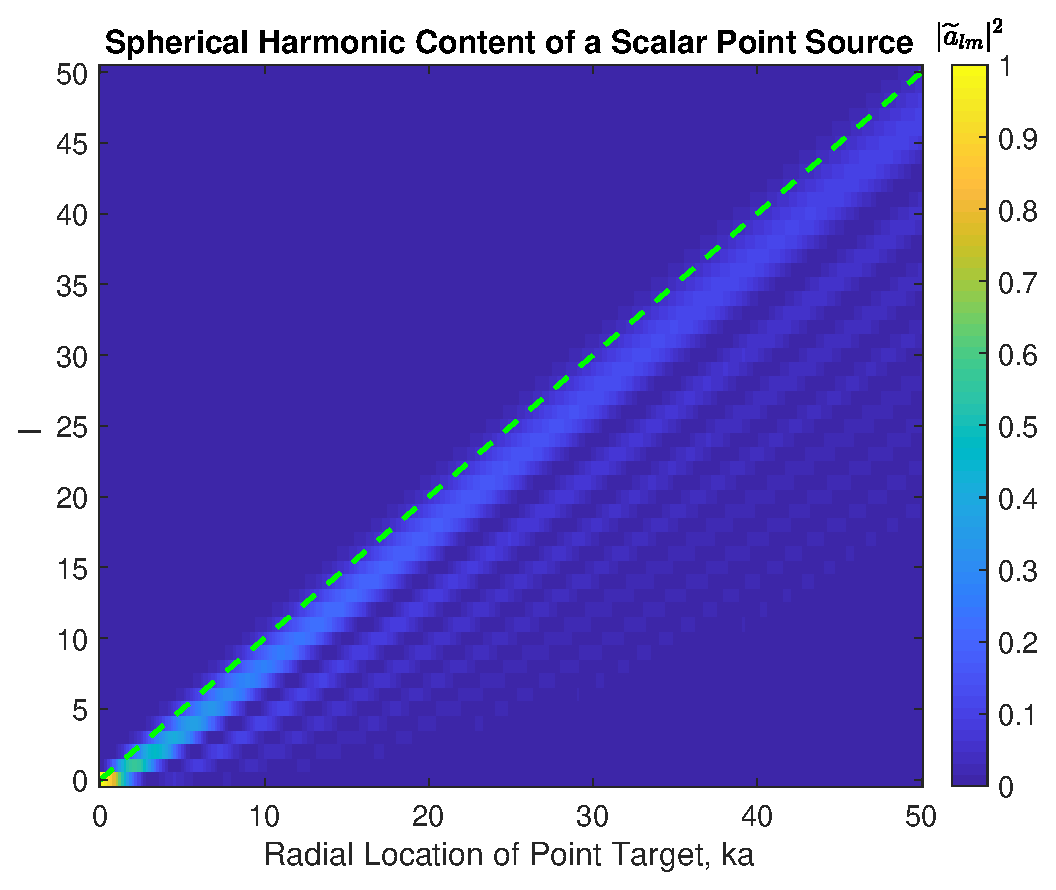
\includegraphics[width=3in]{WaveFunctions/Figures/sphharmcont}}
     \subfigure{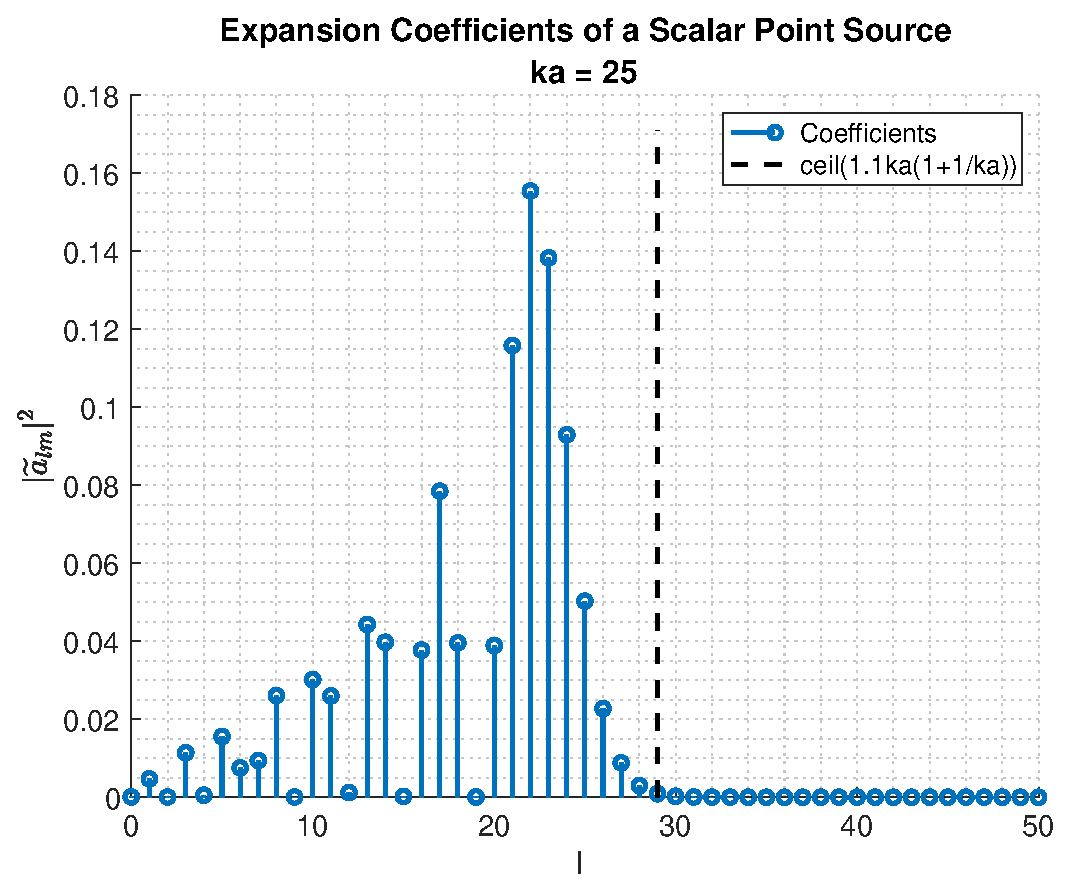
\includegraphics[width=3in]{WaveFunctions/Figures/sphharmcontex}}
  \end{tabular}
  \label{sphharmcont}
\caption{Spherical harmonic content of a scalar point source at $z = a$. Left: coefficients vs $ka$ with the line $l = ka$ plotted. Right: example of $ka = 25$ with \eqref{LLmax} plotted.}
\end{figure}












\chapter{Rotation}
\label{chap:rotation}


\vspace{-7mm}
This chapter gives routines for computing rotation matrices that operate on the expansion coefficients of spherical harmonics and spherical wave functions in order to rotate fields or view fields from a rotated frame.  The rotation matrices work the same for any of the wave functions in Chapter \ref{chap:wavefunctions}.

\section{Euler Rotation}
3D rotation of a Cartesian reference frame can be accomplished with three Euler angles $(\alpha,\beta,\gamma)$, where the sequence rotates the frame successively about one of its axes. The angles can take any value of radians. The most common rotation sequence is denoted Z-X'-Z'', sometimes just called ZXZ. This consists of a right-handed rotation of $\alpha$ about the $z$ axis, followed by a right-handed rotation of $\beta$ about the $x$ axis of the rotated frame (X'), followed by a right-handed rotation of $\gamma$ about the $z$ axis of the rotated frame (Z''). This is represented in a rotation matrix as:
\ea{
\bb{R}_{ZX'Z''}(\alpha,\beta,\gamma) &=& \bb{R}_{Z}(\alpha)\bb{R}_{X}(\beta)\bb{R}_{Z}(\gamma) \\
\ &= &
 \thbth{\cos(\alpha)}{-\sin(\alpha)}{0} {\sin(\alpha)}{ \cos(\alpha)}{ 0} {0}{ 0}{ 1}\thbth{1}{ 0}{ 0}{0 }{\cos(\beta)}{ -\sin(\beta)}{0}{ \sin(\beta) }{\cos(\beta)}\thbth{\cos(\gamma)}{ -\sin(\gamma)}{ 0} {\sin(\gamma)}{ \cos(\gamma) }{0}  {0 }{0 }{1} \label{rot}
}
Each matrix is a right-handed rotation about the axes of the unrotated, or fixed, global frame. The reason the matrices are applied in what seems like reverse order, and applied about the axes of the fixed frame, is because each matrix stacks the rotations in front of it to create the effect that each rotation was applied about the axes of the rotated frame in the order $(\alpha,\beta,\gamma)$.

\begin{figure}[H] 
   \centering
   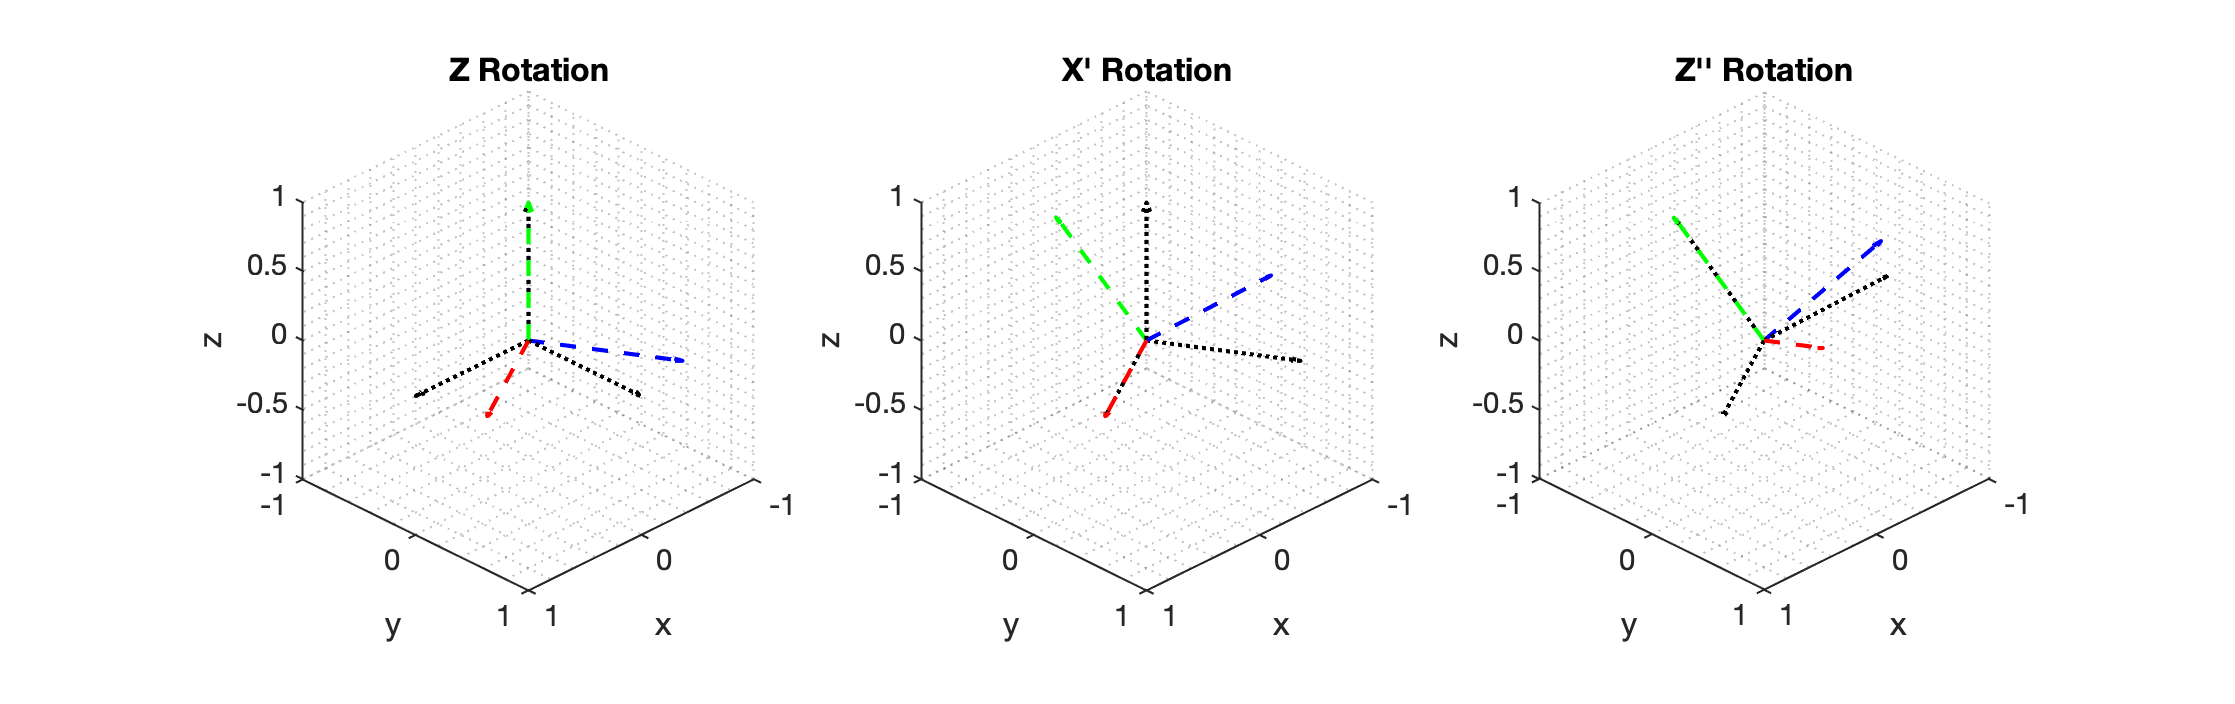
\includegraphics[width=6.5in]{Rotation/Figures/ZXZ} 
   \caption{ZX'Z'' rotation sequence $(\alpha,\beta,\gamma) = (\pi/6, \pi/5, \pi/4)$.  First pane shows the rotation of $\alpha$ about the $z$ axis from the original Cartesian frame (black dotted) to the new frame (red/blue/green). Second pane shows the second rotation of $\beta$ about the $x$ axis of the previously rotated frame. Third pane shows the final rotation of $\gamma$ about the $z$ axis of the previously rotated frame.}
   \label{fig1}
\end{figure}


A point $\bb{x} = [x, y, z]^t$ that in the global frame is rotated to the point $\bb{x}' = [x',y',z']^t$ as
\begin{equation}
\bb{x}' = \bb{R}\bb{x}
\end{equation}

\noindent In other words, the point is rotated through the global frame as though you are standing in the global frame. We call this a forward rotation. $\bb{R}$ is unitary, so the inverse is equal to the transpose, and 
\begin{equation}
\bb{x} = \bb{R}^t\bb{x}'
\end{equation}

The inverse rotation brings the point back, and applies the Euler angles in the reverse order and reverse direction. Given a forward set of angles $(\alpha,\beta,\gamma)$, applying the inverse is equivalent to fixing a point in the global frame and seeing it as you ride along with the rotating frame. We call this the inverse rotation.

Determining the ZXZ Euler angles from a rotation matrix is done with 
\begin{eqnarray}
\alpha & =& \arctan \dfrac{R_{13}}{-R_{23}} \\
\beta & =& \arctan \dfrac{\sqrt{R_{13}^2 + R_{23}^2} }{R_{33}}\\
\gamma &=& \arctan \dfrac{R_{31}}{R_{32}} 
\end{eqnarray}

\noindent where $R_{ij}$ are the matrix entries of $\bb{R}$. 

The rotation matrix and Euler angle conversions are given in the routines \texttt{euler2rot} and \texttt{rot2euler}. A plotting function,  \texttt{plotrot}, not copied here, will plot the axes of the rotated frame given $\bb{R}$. 

{\footnotesize
\VerbatimInput{\code/Rotation/euler2rot.m}
}

{\footnotesize
\VerbatimInput{\code/Rotation/rot2euler.m}
}

%{\footnotesize
%\VerbatimInput{\code/Rotation/plotrot.m}
%}



\clearpage
\section{Rotation Addition Theorem}

The rotation addition theorem for spherical harmonics is given by  
\begin{equation}
Y_{lm}(\theta,\phi) = \sum_{p=-l}^{l} D_{lmp}(\alpha,\beta,\gamma) Y_{lp}(\theta',\phi')
\end{equation}

\noindent where $(\alpha,\beta,\gamma)$ are the three Euler angles describing a ZXZ rotation from unprimed to primed coordinate systems. $D_{lmp}$ is the rotation matrix for spherical harmonics. Because the coordinate $r$ and the gradient are invariant under rotation, the rotation addition theorem for scalar and vector wave functions have identical forms \cite{edmonds1996angular,hansen1988spherical,stein1961addition,dufva2008unified},
\begin{equation}
\psi_{lm}(r,\theta,\phi) = \sum_{p=-l}^{l} D_{lmp}(\alpha,\beta,\gamma) \psi_{lp}(r',\theta',\phi')
\end{equation}
\begin{equation}
\bb{M}_{lm}(r,\theta,\phi) = \sum_{p=-l}^{l} D_{lmp}(\alpha,\beta,\gamma)\bb{M}_{lp}'(r',\theta',\phi')
\end{equation}

This means that the same $D_{lmp}$ can be used to rotate any of following: spherical harmonics, scalar spherical wave functions, vector spherical harmonics, or vector spherical wave functions. $D_{lmp}$ is a square block diagonal matrix with blocks that span $m$ and $p$ for a given $l$, zero otherwise.  Specifically,
\begin{equation}
D_{lmp}(\alpha,\beta,\gamma) = e^{im\alpha}d_{lmp}(\beta)e^{ip\gamma} \label{dlmpsep}
\end{equation}

The rotation matrix is inherently separable in $(\alpha,\beta,\gamma)$, where $\alpha$, and $\gamma$ are diagonal. The matrix $d_{lmp}(\beta)$, called "little-d", is block diagonal and can be computed itself. This is advantageous when precomputing rotation matrices over many combinations of Euler angles. The matrix $d_{lmp}(\beta)$ is given by 
\begin{eqnarray}
d_{lmp}(\beta) &=&  i^{m-p}\sqrt{\dfrac{(l+p)!(l-p)!}{(l+m)!(l-m)!}} \sum_s (-1)^{s}  {l+m \choose l+p-s} {l-m \choose s}  \left(\cos\frac{\beta}{2}\right)^{2l+p-m-2s}\left(\sin\frac{\beta}{2}\right)^{m-p+2s}  \label{dlmpdirect}
\end{eqnarray}


The sum is over all $s$ for positive arguments of the binomial coefficients. There is a version used in quantum mechanics, \cite{wigner2012group}, based on a ZYZ rotation that yields a real-valued $d_{lmp}(\beta)$ matrix. This forms the basis of a recursion algorithm in Section \ref{littled}. The mapping from complex ZXZ  $d_{lmp}(\beta)$ to the purely real ZYZ is, \cite{littledconversion},
\eq{ d_{lmp}^{ZYZ}(\beta)   =  (-i)^{p-m} d_{lmp}^{ZXZ}(\beta)   \label{zyzzxzconv} }
%\eq{ d_{lmp}^{ZYZ}(\beta)   = i^{p-m} (-1)^{p-m} d_{lmp}^{ZXZ}(\beta)   \label{zyzzxzconv} }



%
%\begin{eqnarray}
%d_{lmp}(\beta) &=&  \sqrt{\frac{(l+p)!(l-p)!}{(l+m)!(l-m)!}}\sum_u {l+m \choose l-p-u}{l-m \choose u} \nonumber \\
%\ & \ & \cdot (-1)^{l-p-u}\left(\cos\frac{\beta}{2}\right)^{m+p+2u}\left(\sin\frac{\beta}{2}\right)^{2l-m-p-2u} 
%\end{eqnarray}
%
%The sum is over all $u$ for positive arguments of the binomial coefficients.  


%From Wikipedia ("Wigner-D Matrix"), the rotation matrix is given as
%\eq{D_{lmp}(\alpha\beta\gamma) = e^{-im\alpha}d_{lmp}(\beta)e^{-ip\gamma}}
%
%with 
%\begin{eqnarray}
%d_{lmp}(\beta) &=&  \sqrt{(l+m)!(l-m)!(l+p)!(l-p)!} \sum_s  \dfrac{(-1)^{m-p+s}}{(l+p-s)!s!(m-p+s)!(l-m-s)!} \nonumber \\
%\ & \ & \cdot  \left(\cos\frac{\beta}{2}\right)^{2l+p-m-2s}\left(\sin\frac{\beta}{2}\right)^{m-p+2s} 
%\end{eqnarray}

%\begin{eqnarray}
%d_{m'm}^j(\beta) &=&  \sqrt{(j+m')!(j-m')!(j+m)!(j-m)!} \sum_s  \dfrac{(-1)^{m'-m+s}}{(j+m-s)!s!(m'-m+s)!(j-m'-s)!} \nonumber \\
%\ & \ & \cdot  \left(\cos\frac{\beta}{2}\right)^{2j+m-m'-2s}\left(\sin\frac{\beta}{2}\right)^{m'-m+2s} 
%\end{eqnarray}
%
%This is for a ZYZ rotation, which results in the purely real $d_{lmp}$.  For ZXZ Euler rotations, the $(-1)^{m-p+s}$ is replaced with $(-1)^s i^{p-m}$ and $s$ runs from $[0,l+p]$ while for valid factorials.  However, I found that $(-1)^s i^{m-p}$ and multiplying the diagonal matrices in reverse (conjugate transpose) as $e^{im\gamma}d_{lmp}(\beta)e^{ip\alpha}$ matched the values given by the recursion algorithm above. Therefore, the transform between the purely real and complex  $d_{lmp}(\beta)$ is 
%\eq{ d_{lmp}(\beta) \leftarrow i^{m-p} (-1)^{m-p} d_{lmp}(\beta)}
%


%\begin{eqnarray}
%d_{lmp}(\beta) &=&  \sqrt{(l+m)!(l-m)!(j+p)!(j-p)!} \sum_s  \dfrac{(-1)^{m-p+s}}{(l+p-s)!s!(m-p+s)!(l-m-s)!} \nonumber \\
%\ & \ & \cdot  \left(\cos\frac{\beta}{2}\right)^{2l+p-m-2s}\left(\sin\frac{\beta}{2}\right)^{m-p+2s}  \\
%\ &=&  \sqrt{\dfrac{(l+p)!(l-p)!}{(l+m)!(l-m)!}} \sum_s  \dfrac{(-1)^{m-p+s} (l+m)!(l-m)! }{(l+p-s)!s!(m-p+s)!(l-m-s)!}   \left(\cos\frac{\beta}{2}\right)^{2l+p-m-2s}\left(\sin\frac{\beta}{2}\right)^{m-p+2s}  \\
%\ &=&  \sqrt{\dfrac{(l+p)!(l-p)!}{(l+m)!(l-m)!}} \sum_s (-1)^{m-p+s}  {l+m \choose l+p-s} {l-m \choose s}  \left(\cos\frac{\beta}{2}\right)^{2l+p-m-2s}\left(\sin\frac{\beta}{2}\right)^{m-p+2s} 
%\end{eqnarray}




\subsection{Field Rotations} 

Given a field expansion in an unprimed system, 
\begin{equation}
\bb{E}(\bb{r}) = \sum_{lm}a_{lm}\bb{M}_{lm}(k,\br)+b_{lm}\bb{N}_{lm}(k,\br)
\end{equation}

the expansion coefficients in the primed system are found by substituting the addition theorem 

\begin{equation}
\bb{E}'(\bb{r}') = \sum_{lp}a_{lp}'\bb{M}_{lp}'(k,\br')+b_{lp}'\bb{N}_{lp}'(k,\br')
\end{equation}

\noindent where 

\begin{equation}
a_{lp}' = \sum_m a_{lm}D_{lmp}, \quad \quad
b_{lp}' = \sum_m b_{lm}D_{lmp}
\end{equation}

In matrix form, if $\bb{a}$ are the outgoing wave coefficients in the $i$ frame, and $\bb{a}'$ are those in the rotated $i'$ frame, then 
\begin{equation}
\bb{a}' = \bb{D}_i\bb{a}
\end{equation}

\noindent where $\bb{D}_i$ is the rotation matrix, and $(\alpha,\beta,\gamma)$ describe the rotation from $i$ to $i'$.  In other words, the application of $\bb{D}_i$ is an inverse rotation on the field (the coefficients $\bb{a}'$ describe the same field but viewed from the rotated frame). $\bb{D}_i$ is unitary, so the inverse is the conjugate transpose: $\bb{D}_i^{-1} = \bb{D}^*_i$.  This is the forward rotation, where the field itself rotates, to follow the Euler angles, as seen from the originating frame. 

%, and the inverse relation is 
%
%\begin{equation}
%\bb{a} = \bb{D}^*_i\bb{a}'
%\end{equation}


\subsection{Properties} 

Here we give several properties of the rotation matrix. The transpose satisfies the following relation
\eq{D_{lmp}(\alpha,\beta,\gamma) = D_{lpm}^*(-\gamma+\pi,\beta,-\alpha+\pi) }
The following relation exists for conjugated matrix elements
\eq{D_{l,-m,-p} = (-1)^{m+p}D_{lmp}^*}

The following identity exists between the $d_{lmp}(\beta)$ and the Legendre polynomials
\ea{d_{l00}(\beta) &=& P_l(\cos\beta) }

The rotation matrix is orthogonal over the three Euler angles as
\eq{\int_{0}^{2\pi} \int_{0}^{\pi} \int_{0}^{2\pi} D_{l'm'p'}^*(\alpha,\beta,\gamma) D_{lmp}(\alpha,\beta,\gamma) d\alpha \sin\beta d\beta d\gamma
= \dfrac{8 \pi^2}{2 l + 1} \delta_{l'l}\delta_{m'm}\delta_{p'p}}

where 
\eq{\int_{0}^{2\pi}  d\alpha \int_{0}^{\pi} \sin\beta d\beta  \int_{0}^{2\pi} d\gamma
= 8 \pi^2}

The same integral computed over a matrix element is 
\ea{I_{lmp} &=& \int_{0}^{2\pi} \int_{0}^{\pi} \int_{0}^{2\pi} D_{lmp}(\alpha,\beta,\gamma) d\alpha \sin\beta d\beta d\gamma \\
\ &=& 4\pi^2 \delta_{m,0}  \delta_{p,0} \int_{0}^{\pi}d_{lmp}(\beta) \sin\beta d\beta  \\
\ &=& 4\pi^2 \delta_{m,0}  \delta_{p,0}\int_{0}^{\pi}P_l(\cos\beta) \sin\beta d\beta  \\ 
\ &=& 8 \pi^2 \delta_{l,0}\delta_{m,0}  \delta_{p,0} }

For $\alpha = 0$, $\gamma = 0$, the sum over the diagonal elements of the blocks satisfy
\eq{\sum_{m=-l}^l D_{lmm}(\beta) = \sum_{m=-l}^l d_{lmm}(\beta) = \dfrac{\sin\left(\dfrac{(2 l+1)}{2}\beta\right)}{\sin\left(\dfrac{\beta}{2}\right)}}

which is the normalized Dirichlet kernel.  



\clearpage
\newpage

\section{Computation of $D_{lmp}$}

Direct computation of the rotation matrix using \eqref{dlmpsep} and \eqref{dlmpdirect} is not advised because of the need to compute the binomial coefficients. Instead, a fast recursion algorithm for computing the full $D_{lmp}$ is given in \cite{choi1999rapid}. This begins with a rotation matrix defined
\begin{equation}
(\hat{x},\hat{y},\hat{z}) = (x,y,z)\thbth{R_{xx}}{R_{xy}}{R_{xz}}{R_{yx}}{R_{yy}}{R_{yz}}{R_{zx}}{R_{zy}}{R_{zz}} = (x,y,z)\bb{R}
\end{equation}

which is opposite to the rotation matrix in \eqref{rot}. Next, \cite{choi1999rapid} defines the following matrices 
\begin{equation}
\bb{D} = \bb{F} + i\bb{G}
\end{equation}
\begin{equation}
\bb{F} = \thbth{(R_{yy}+R_{xx})/2}{R_{xz}/\sqrt{2}}{(R_{yy}-R_{xx})/2}{R_{zx}/\sqrt{2}}{R_{zz}}{-R_{zx}/\sqrt{2}}{(R_{yy}-R_{xx})/2}{-R_{xz}/\sqrt{2}}{(R_{yy}+R_{xx})/2}
\end{equation}
\begin{equation}
\bb{G} = \thbth{(R_{yx}-R_{xy})/2}{R_{yz}/\sqrt{2}}{-(R_{yx}+R_{xy})/2}{-R_{zy}/\sqrt{2}}{0}{-R_{zy}/\sqrt{2}}{(R_{yx}+R_{xy})/2}{R_{yz}/\sqrt{2}}{(R_{xy}-R_{yx})/2}
\end{equation}

\noindent which serves as the initial condition
\eq{D_{1mp} = \bb{D}}
%\begin{eqnarray}
%D_{lmp} &=& F_{lmp} + iG_{lmp} \\
%\bb{D}_{1mp} &=& \bb{D}
%\end{eqnarray}

The recursion equations are given as follows: 
\begin{enumerate}
\item For $(-l+1) \leq p \leq (l-1)$:
\begin{equation}
D_{lmp} = a_{lmp}D_{100}D_{l-1,mp}+b_{lmp}D_{110}D_{l-1,m-1,p}+b_{l,-m,p}D_{1,-10}D_{l-1,m+1,p}
\end{equation}
\begin{eqnarray}
a_{lmp} &=& \sqrt{\frac{(l+m)(l-m)}{(l+p)(l-p)}} \\
b_{lmp} &=& \sqrt{\frac{(l+m)(l+m-1)}{2(l+p)(l-p)}} 
\end{eqnarray}
$p = \pm l$ is not covered, $a_{lmp} = 0$ for $m=\pm l$, and $b_{lmp} = 0$ for both $m=-l$ and $m=-l+1$.

\item For $-l \leq p \leq (l-2)$:
\begin{eqnarray}
D_{lmp} &=& c_{lm,-p}D_{10,-1}D_{l-1,m,p+1}+d_{lm,-p}D_{11,-1}D_{l-1,m-1,p+1} \nonumber \\
\ & \ & +d_{l,-m,-p}D_{1,-1,-1}D_{l-1,m+1,p+1}
\end{eqnarray}
\begin{eqnarray}
c_{lmp} &=& \sqrt{\frac{2(l+m)(l-m)}{(l+p)(l+p-1)}} \\
d_{lmp} &=& \sqrt{\frac{(l+m)(l+m-1)}{(l+p)(l+p-1)}} 
\end{eqnarray}
$p = \pm l$ and $p=(l-1)$ are not covered, $c_{lmp} = 0$ for $m=\pm l$, and $d_{lmp} = 0$ for both $m=-l$ and $m=-l+1$.

\item For $(-l+1) \leq p \leq l$:
\begin{eqnarray}
D_{lmp} &= &c_{lm,p}D_{101}D_{l-1,m,p-1}+d_{lm,p}D_{111}D_{l-1,m-1,p-1} \nonumber \\
\ & \ & +d_{l,-m,p}D_{1,-1,1}D_{l-1,m+1,p-1}
\end{eqnarray}
$p = -l$ and $p = -l+1$ are not covered, and $c_{lmp}$ and $d_{lmp}$ are the same as above.
\end{enumerate}

This algorithm is the basis for two routines that follow. The first routine computes \texttt{Dlmp} on a full square matrix, which has mostly zero elements. The second routine is specialized to compute this on a sparse 1D array to same memory.  

\subsection{Full $D_{lmp}$ Matrix}

The routine \texttt{Dlmp} returns the rotation matrix in full, including zeros, starting with $l=1$. As mentioned, this describes an inverse rotation. Use the string switch \texttt{'mono'} to include the monopole term. The algorithm above uses a rotation matrix that is transposed from our convention, so we transpose it on input to keep the routine consistent. There are helper functions to compute the coefficients: \texttt{a\_lmp}, \texttt{b\_lmp}, \texttt{c\_lmp}, \texttt{d\_lmp}.  Figure \ref{fig1} shows the magnitude of $D_{lmp}$ for different $\beta$ ($\alpha$, $\gamma$ do not affect the magnitude).  

\begin{figure}[H] 
   \centering
   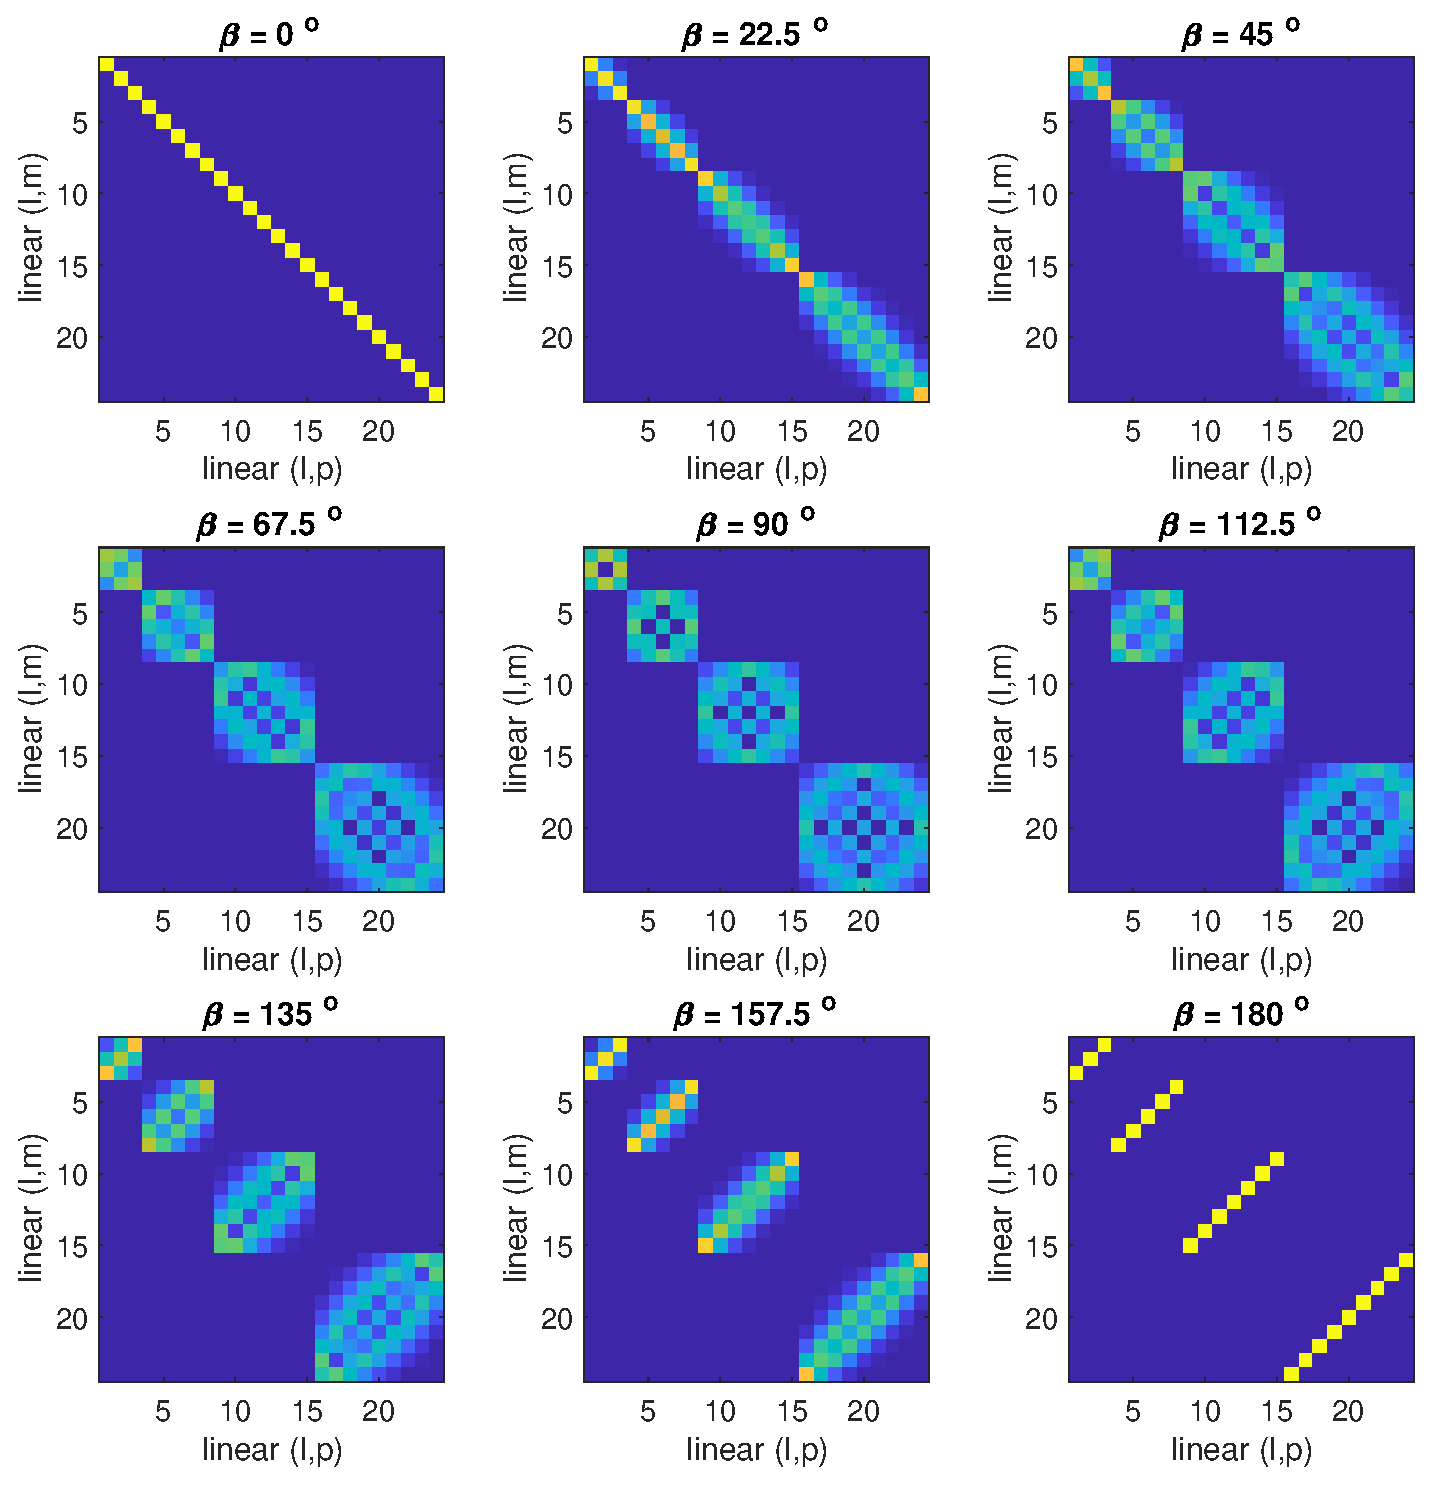
\includegraphics[width=4in]{Rotation/Figures/Dlmp} 
   \caption{$D_{lmp}$ magnitude (color scale [0, 1]) for varying $\beta$, $\alpha = \gamma = 0$.}
   \label{fig1}
\end{figure}

{\footnotesize
\VerbatimInput{\code/Rotation/Dlmp.m}
}


\newpage

\subsection{Sparse $D_{lmp}$ Matrix}

The rotation matrix that is the output of \texttt{Dlmp} should not be used directly for matrix-vector multiplication because it contains unnecessary zeros. The quick fix is to immediately transform it to a sparse matrix:

\begin{verbatim}
      D = sparse(Dlmp(L,alpha,beta,gamma));
\end{verbatim}

If several different rotation matrices are needed, they will likely have different numbers of non-zero elements, which can lead to problems with preallocation. Furthermore, the routine \texttt{Dlmp} works on a large, mostly zero, 2D matrix. Therefore, we have a modified version of the routine \texttt{Dlmp}, which recurses on a sparse matrix stored as a 1D array. The modifications follow.

Because the rotation matrix is square block diagonal, the maximum number of non-zero elements (excluding the monopole) is found by counting the elements in blocks that are sized $2l+1$ on a side up to a maximum degree harmonic $L$: 
\begin{eqnarray}
N_L &=& \sum_{l=1}^L (2l + 1)^2  \\
\ &=& 4 \sum_{l=1}^L l^2 + 4 \sum_{l=1}^L l + \sum_{l=1}^L 1 \\
%\ &=& 4 \left(\dfrac{L^3}{3} + \dfrac{L^2}{2} + \dfrac{L}{6}\right) + 4\left(\dfrac{L^2 + L}{2}\right) + L \\
\ &=& \dfrac{4}{3} L^3 + 4L^2 + \dfrac{11}{3}L 
\end{eqnarray}

Add 1 for the monopole.  Next, we map the 2D row/column linear indices to a 1D index of the sparse matrix. Let the row linear index for the $(l,m)$ harmonic in the full matrix be $l^2 + l + m$ and let the column linear index of the $(l,p)$ harmonic in the full matrix be $l^2 + l + p$.  Counting column-major (top-down, left-right), the linear index for the $(l,m,p)$ element in the sparse array is
\begin{equation}
I(l,m,p) = N_{l-1} + (2l+1)(l+p) + (l+m+1)
\end{equation}

\noindent The term $N_{l-1}$ counts the number of elements for all full blocks less than $l$, the second term counts the number of elements in full columns of the current block less than $p$, the last term counts the rows up to $m$ in the current column.  Again, add 1 for the monopole.  

The routine \texttt{DlmpSparse} returns the three column arrays containing the row index, column index, and matrix entries of $D_{lmp}$. It is the same as \texttt{Dlmp} except computed on a 1D array.  Use the string switch \texttt{'mono'} for the monopole.  The two helper functions \texttt{NDlmpSparse} and \texttt{indDlmpSparse} return the number of elements and index for the sparse rotation matrix. A further refinement could use conjugate symmetry to only store half of the matrix plus the main diagonal, but that then requires specialized routines for matrix-vector multiplication. Finally, the helper functions as written create a bottleneck, so a faster version, \texttt{DlmpSparseFast}, is included but not copied here. This uses inline indexing and is about five times faster for moderate values of $L$. 


{\footnotesize
\VerbatimInput{\code/Rotation/DlmpSparse.m}
}


{\footnotesize
\VerbatimInput{\code/Rotation/NDlmpSparse.m}
}


{\footnotesize
\VerbatimInput{\code/Rotation/indDlmpSparse.m}
}


\newpage

\section{Computation of $d_{lmp}(\beta)$}
\label{littled}
This section contains routines for the computation of "little-d", $d_{lmp}(\beta)$. This rotation matrix should be used with \eqref{dlmpsep} to precompute and loop over combinations of Euler angles.  Four routines are provided. The first is a direct computation for cross-checking, but should not be used in practice because computing the factorials in the binomial coefficients is not accurate. The second is based on a fast recursion of the purely real ZYZ $d_{lmp}(\beta)$, computed on the full matrix, then converted to complex ZXZ $d_{lmp}(\beta)$.  The third routine is the same as the second but faster. The last routine is the same as the second but computed on the sparse matrix using the sparse indexing tools developed before. 


\subsection{Direct Computation}

The routine \texttt{dlmpBetaDirect} computes the ZXZ complex $d_{lmp}(\beta)$ directly from \eqref{dlmpdirect}. This is good to maybe $L = 20$ due to direct computation of the factorials. This is used to validate the recursive algorithms.

{\footnotesize
\VerbatimInput{\code/Rotation/dlmpBetaDirect.m}
}

\subsection{Recursion Algorithm}

A fast computation of $d_{lmp}(\beta)$ is based on the recursive algorithm in \cite{gimbutas2009fast}, which gives an algorithm for the purely real ZYZ matrix. The recursion equations for real $d_{lmp}(\beta)$ are 
\ea{d_{lmp} &=& \cos^2 (x) A_{lmp} d_{l-1,m-1,p-1} - 2 \sin (x)\cos (x) B_{lmp} d_{l-1,m-1,p} + \sin^2 (x) C_{lmp} d_{l-1,m-1,p+1} \label{dlmprec1} \\
 d_{lmp} &=& \sin^2 (x)  D_{lmp} d_{l-1,m+1,p-1}+2 \sin (x) \cos (x)  E_{lmp} d_{l-1,m+1,p} + \cos^2 (x)  F_{lmp} d_{l-1,m+1,p+1} \label{dlmprec2} \\
 d_{lmp} &=& \sin (x) \cos (x)  G_{lmp} d_{l-1,m,p-1}+(\cos^2 (x)  - \sin^2 (x) ) H_{lmp} d_{l-1,m,p} -\sin (x)\cos (x)  I_{lmp} d_{l-1,m,p+1} \nonumber \label{dlmprec3} \\}
 
\noindent where $x = \beta/2$. The coefficients can be written as an outer product 
\eq{\thbth{A_{lmp}^2}{B_{lmp}^2}{C_{lmp}^2}{D_{lmp}^2}{E_{lmp}^2}{F_{lmp}^2}{G_{lmp}^2}{H_{lmp}^2}{I_{lmp}^2} =  \thrcol{\dfrac{1}{(l+m)(l+m-1)} }{\dfrac{1}{(l-m)(l-m-1)} }{\dfrac{1}{(l-m) (l+m)} } \thrrow{(l+p)(l+p-1)}{(l+p)(l-p)}{(l-p)(l-p-1) } }

%A_{lmp} &=& \sqrt{\dfrac{(l+p)(l+p-1) }{(l+m)(l+m-1) } } \\
%B_{lmp} &=& \sqrt{\dfrac{(l+p)(l-p) }{(l+m)(l+m-1) } } \\
%C_{lmp} &=& \sqrt{\dfrac{(l-p)(l-p-1) }{(l+m)(l+m-1) } } \\
%D_{lmp} &=& \sqrt{\dfrac{(l+p)(l+p-1) }{(l-m)(l-m-1) } }  \\
%E_{lmp} &=& \sqrt{\dfrac{(l+p)(l-p) }{(l-m)(l-m-1) } }  \\
%F_{lmp} &=& \sqrt{\dfrac{(l-p)(l-p-1) }{(l-m)(l-m-1) } }  \\
%G_{lmp} &=& \sqrt{\dfrac{(l+p)(l+p-1) }{(l-m) (l+m)} }  \\
%H_{lmp} &=&\sqrt{\dfrac{(l+p)(l-p) }{(l-m)(l+m) } }   \\
%I_{lmp} &=&  \sqrt{\dfrac{(l-p)(l-p-1) }{(l-m)(l+m) } }  }



%
%\ea{d_{n}^{m',m} &=& \cos^2 (x) A d_{n-1}^{m'-1,m-1} - 2 \sin (x)\cos (x) B d_{n-1}^{m'-1,m} + \sin^2 (x) C d_{n-1}^{m'-1,m+1} \label{dlmprec1} \\
% d_{n}^{m',m} &=& \sin^2 (x)  D d_{n-1}^{m'+1,m-1}+2 \sin (x) \cos (x)  E d_{n-1}^{m'+1,m} + \cos^2 (x)  F d_{n-1}^{m'+1,m+1} \label{dlmprec2} \\
% d_{n}^{m',m} &=& \sin (x) \cos (x)  G d_{n-1}^{m',m-1}+(\cos^2 (x)  - \sin^2 (x) ) H d_{n-1}^{m',m} -\sin (x)\cos (x)  I d_{n-1}^{m',m+1} \nonumber \label{dlmprec3} \\}
%\ea{x &=& \beta/2\\
%A_{nm'm} &=& \sqrt{\dfrac{(n+m)(n+m-1) }{(n+m')(n+m'-1) } } \\
%B_{nm'm} &=& \sqrt{\dfrac{(n+m)(n-m) }{(n+m')(n+m'-1) } } \\
%C_{nm'm} &=& \sqrt{\dfrac{(n-m)(n-m-1) }{(n+m')(n+m'-1) } } \\
%D_{nm'm} &=& \sqrt{\dfrac{(n+m)(n+m-1) }{(n-m')(n-m'-1) } }  \\
%E_{nm'm} &=& \sqrt{\dfrac{(n+m)(n-m) }{(n-m')(n-m'-1) } }  \\
%F_{nm'm} &=& \sqrt{\dfrac{(n-m)(n-m-1) }{(n-m')(n-m'-1) } }  \\
%G_{nm'm} &=& \sqrt{\dfrac{(n+m)(n+m-1) }{(n-m') (n+m')} }  \\
%H_{nm'm} &=&\sqrt{\dfrac{(n+m)(n-m) }{(n-m')(n+m') } }   \\
%I_{nm'm} &=&  \sqrt{\dfrac{(n-m)(n-m-1) }{(n-m')(n+m') } }  }
%
%In the paper, the numerator for $I$ is $(n-m+1)$, which is incorrect. I found $(n-m-1)$ to be correct, which also preserves the symmetry, so that these can be written as an outer product as 
%\eq{\thbth{A^2}{B^2}{C^2}{D^2}{E^2}{F^2}{G^2}{H^2}{I^2} =  \thrcol{\dfrac{1}{(n+m')(n+m'-1)} }{\dfrac{1}{(n-m')(n-m'-1)} }{\dfrac{1}{(n-m') (n+m')} } \thrrow{(n+m)(n+m-1)}{(n+m)(n-m)}{(n-m)(n-m-1) } }

The recursion algorithm first computes \eqref{dlmprec1} for $m=l$ and all $\pm p$, then \eqref{dlmprec2} for $m=-l$ all $p$, and finally \eqref{dlmprec3} for $m=(-l+1),...,(l-1)$ all $p$.  When a coefficient is zero, the corresponding term at $l-1$ does not exist and can be ignored.  With the conversion to complex using \eqref{zyzzxzconv}, this recursion matches the direct compuation and matches the full \texttt{Dlmp} for $(\alpha,\beta,\gamma) = (0,\beta,0)$.  Note, in \cite{gimbutas2009fast}, the numerator of $I_{lmp}$ has $(l-p+1)$, which is incorrect. It should be $(l-p-1)$, so that it preserves the symmetry of the coefficients. 

The routine \texttt{dlmpBeta} is a straight implementation of \eqref{dlmprec1}, \eqref{dlmprec2}, \eqref{dlmprec3} on the full matrix (with zeros) with conversion to complex.  Use \texttt{'mono'} to include the monopole. A second version of this routine, \texttt{dlmpBetaFast}, which is not copied here but included in the library, is a faster implementation that uses inline indexing, inline coefficient computation, and vectorized real to complex conversion. Still on the full matrix, it runs about six times faster.

{\footnotesize
\VerbatimInput{\code/Rotation/dlmpBeta.m}
}

\subsection{Sparse Recursive}
Like the full $D_{lmp}$, $d_{lmp}(\beta)$ can be computed as a sparse matrix on a 1D array with proper bookkeeping to avoid having to create and index a large matrix of zeros.  We solved the problem of indexing the sparse rotation matrix before.  \texttt{dlmpBetaSparse} is a version of \texttt{dlmpBeta} that returns the row, column and matrix entries for sparse complex ZXZ $d_{lmp}(\beta)$.  

{\footnotesize
\VerbatimInput{\code/Rotation/dlmpBetaSparse.m}
}


%
%\subsubsection{Log-recurrence for $d_{lmp}(\beta)$} 
%We'll derive a recurrence based on the log-transform to compute each matrix element directly. This means including the factorials out front so that they cancel with the factorials in the sum.
%
%\begin{eqnarray}
%d_{lmp}(\beta) &=&  \sum_s (-1)^s i^{m-p}  \dfrac{\sqrt{(l+p)!(l-p)!(l+m)!(l-m)! }}{(l+p-s)!(m-p+s)! s! (l-m-s)!}  \left(\cos\frac{\beta}{2}\right)^{2l+p-m-2s}\left(\sin\frac{\beta}{2}\right)^{m-p+2s} 
%\end{eqnarray}
%
%or 
%\begin{eqnarray}
%d_{lmp}(\beta) &=& i^{m-p}  \sum_s (-1)^s  e^{\ln a_s} 
%\end{eqnarray}
%where
%\eq{a_s = c d_{s}  C_{s} S_{s}  }
%
%\ea{c &=& \sqrt{(l+p)!(l-p)!(l+m)!(l-m)! } \\
%d_{s} &=& \dfrac{1}{(l+p-s)!(m-p+s)! s! (l-m-s)!} \\
%C_{s} &=& \left(\cos\frac{\beta}{2}\right)^{2l+p-m-2s}\\
%S_{s} &=& \left(\sin\frac{\beta}{2}\right)^{m-p+2s} }
%
%Taking the natural log
%\eq{\ln a_s = \ln c + \ln d_{s} + \ln C_{s} + \ln S_{s}  }



\chapter{Translation}
\label{chap:translation}

\vspace{-5mm}
This chapter gives routines for computing translation matrices that operate on the spherical wave function expansions given in Chapter \ref{chap:wavefunctions}. Translation matrices, which are derived from addition theorems, allow us to represent a scalar or vector field in two different but parallel reference frames. The frame of reference is being translated, not the field. The addition theorems and matrix diagonalization are first outlined. Next, algorithms and routines for the scalar axial translation matrices (i.e., translation along the $z$-axis) are given which are computed on full or sparse matrices. Last, algorithms and routines for full and sparse vector axial translation matrices are derived from the scalar versions.  

\vspace{-2mm}
\section{Translation Addition Theorem}

The translation addition theorems for spherical wave functions allow the same field to be expanded in two different, but parallel, frames. These are given for scalar waves as \cite{chew1995waves}, 
\begin{eqnarray}
\psi_{l'm'}(k,\br_i) &=& \sum_{l=0}^{\infty}\sum_{m=-l}^{l} \alpha^{ji}_{lm,l'm'} \textit{Rg}\psi_{lm}(k,\br_j), \quad \quad r_j < r_{ji} \label{adthmscal1} \\
\psi_{l'm'}(k,\br_i) &=& \sum_{l=0}^{\infty}\sum_{m=-l}^{l} \beta^{ji}_{lm,l'm'}\psi_{lm}(k,\br_j), \quad \quad r_j > r_{ji} \label{adthmscal2}\\
\textit{Rg}\psi_{l'm'}(k,\br_i) &=& \sum_{l=0}^{\infty}\sum_{m=-l}^{l} \beta^{ji}_{lm,l'm'}\textit{Rg}\psi_{lm}(k,\br_j), \quad \quad \forall r_j \label{adthmscal3}  
\end{eqnarray}

\noindent where $\beta^{ji}_{lm,l'm'} = \textit{Rg} \alpha^{ji}_{lm,l'm'}$ are translation matrices and $\textit{Rg}$ is the regular part. The position vectors, $\br_i$ and $\br_j$, are measured from the origins of each frame. The first relation expands radiating waves from frame $i$ as regular or incoming waves in frame $j$. The second expands radiating waves in frame $i$ as radiating waves in frame $j$. The last expresses regular waves in frame $i$ and regular waves in frame $j$. Each addition theorem has a different region of validity: \eqref{adthmscal1} is valid within a sphere of radius $r_{ji} = \vert \bb{r}_{ji} \vert = \vert \br_j- \br_i\vert$ centered on frame $j$; \eqref{adthmscal2} is valid outside a radius $r_{ji}$ centered on frame $j$; \eqref{adthmscal3}  is valid everywhere. 

Translation addition theorems for vector spherical wave functions have similar structures, \cite{chew1995waves}. The first is 
\begin{eqnarray}
\bb{M}_{l'm'}(k,\br_i) &=& \sum_{l=1}^{\infty}\sum_{m=-l}^{l} A^{ji}_{lm,l'm'} \textit{Rg}\bb{M}_{lm}(k,\br_j),  + B^{ji}_{lm,l'm'} \textit{Rg}\bb{N}_{lm}(\br_j) \\
\bb{N}_{l'm'}(k,\br_i) &=& \sum_{l=1}^{\infty}\sum_{m=-l}^{l} B^{ji}_{lm,l'm'} \textit{Rg}\bb{M}_{lm}(k,\br_j),  + A^{ji}_{lm,l'm'} \textit{Rg}\bb{N}_{lm}(\br_j)
\end{eqnarray}

\noindent where $A^{ji}_{lm,l'm'}$ and $B^{ji}_{lm,l'm'}$ are vector translation matrices and is valid for $r_j < r_{ji}$. The remaining two relations are analogous to the scalar case and can be obtained with appropriate Hankel or Bessel functions in $A^{ji}_{lm,l'm'}$ and $B^{ji}_{lm,l'm'}$. These show that vector modes mix when translated. The spherical vector components are also transformed and are expressed relative to the origin of the new frame. This means that the vector components in each frame need to be converted to Cartesian components before comparing.


\begin{figure}[H] 
   \centering
   \includegraphics[width=3.5in]{Translation/Figures/transdiagram} 
   \caption{Coordinate frames $i$ and $j$.}
   \label{translationadd}
\end{figure}


Translation matrices allow us to manipulate field using only the expansion coefficients.  For example, a radiating scalar field is expanded in frame $i$ as 
\begin{equation}
\phi(\br_i) = \sum_{l'=0}^{\infty}\sum_{m'=-l'}^{l'} a_{l'm'} \psi_{l'm'}(\br_i)
\end{equation}

The same field expressed as incoming waves in frame $j$ comes from substituting \eqref{adthmscal1} and regrouping terms as
\begin{eqnarray}
\phi(\br_j) &=& \sum_{l=0}^{\infty}\sum_{m=-l}^{l} b_{lm}  \textit{Rg}\psi_{lm}(k,\br_j) \\
b_{lm} &=& \sum_{l'=0}^{\infty}\sum_{m'=-l'}^{l'} \alpha^{ji}_{lm,l'm'}a_{l'm'}
\end{eqnarray}
%
%\begin{eqnarray}
%\phi(\br_j) &=& \sum_{l'=0}^{\infty}\sum_{m'=-l'}^{l'} a_{l'm'} \sum_{l=0}^{\infty}\sum_{m=-l}^{l} \alpha^{ji}_{lm,l'm'} \textit{Rg}\psi_{lm}(k,\br_j) \nonumber \\
%\ &=& \sum_{l=0}^{\infty}\sum_{m=-l}^{l} b_{lm}  \textit{Rg}\psi_{lm}(k,\br_j) \\
%b_{lm} &=& \sum_{l'=0}^{\infty}\sum_{m'=-l'}^{l'} \alpha^{ji}_{lm,l'm'}a_{l'm'}
%\end{eqnarray}

Likewise, for the other relations. In matrix notation this is 
\begin{eqnarray}
\phi(k,\br_i) &=&  \boldsymbol{\psi}^t(k,\br_i)\cdot \bb{a} \\
\phi(k,\br_j) &=&  \textit{Rg}\boldsymbol{\psi}^t(k,\br_j)\cdot \bb{b} \\
\bb{b} &=& \boldsymbol{\alpha}_{ji} \bb{a}
\end{eqnarray}

The analogous matrix notation for vector waves is
\begin{eqnarray}
\bb{E}(k,\br_i) &=& \rvectwo{\bb{M}^t(k,\br_i)}{\bb{N}^t(k,\br_i)}\cvectwo{\bb{a}}{\bb{b}} \\
\bb{E}(k,\br_j)&=& \rvectwo{\Re\bb{M}^t(k,\br_j)}{\Re\bb{N}^t(k,\br_j)}\cvectwo{\bb{c}}{\bb{d}} \\
\cvectwo{\bb{c}}{\bb{d}}  &=&\tbt{\bb{A}_{ji}}{\bb{B}_{ji}}{\bb{B}_{ji}}{\bb{A}_{ji}}\cvectwo{\bb{a}}{\bb{b}}
\end{eqnarray}

In both scalar and vector cases the transpose, $^t$, means align the harmonic indices along columns. Technically the sums are infinite, but the matrices are always truncated in practice.

\section{Diagonalization}

Explicit expressions for the matrix elements of the scalar and vector translation matrices are given in \cite{chew1995waves}, but are given in terms of Wiger 3-j symbols, which are slow and inaccurate to compute. Fast recursions for quickly computing the scalar and vector translation matrices were developed in \cite{mackowski1991analysis, chew1992recurrence, chew1993efficient}.  

The standard way to compute the translation matrix is to break it into three matrices. The local frame, $i$, is first rotated to point its $z$-axis toward the destination frame, $j$. The local frame is then axially translated. Finally, the frame is then rotated back. This effectively diagonalizes the translation matrix. Specifically, if the vector $\br_{ji}$ points from the origin of frame $i$ to the origin of frame $j$, with magnitude $r_{ji}$ and spherical angles $\theta_{ji}$, $\phi_{ji}$, shown in Figure \ref{translationadd}, then the scalar translation matrix is expanded (diagonalized) as
\begin{equation}
\boldsymbol{\alpha}_{ji} = \bb{D}^*(\phi_{ji}+\pi/2,\theta_{ji},0) \cdot \boldsymbol{\alpha}_z(r_{ji}) \cdot \bb{D}(\phi_{ji}+\pi/2,\theta_{ji},0)
\label{alphazdiag}
\end{equation}

\noindent where $\bb{D}$ is the rotation matrix with ZXZ convention, and $\boldsymbol{\alpha}_z(r_{ji})$ is the axial translation matrix in the $+z$ direction. The factor of $\pi/2$ ensures that $\theta_{ji}$ tips the $z$-axis toward the destination frame with a right-handed X rotation. The sequence starts with an inverse rotation on the right size because we first view the field, which is fixed in the global frame, from the point of view of the rotated frame. Next, this point of view is translated along the $z$-axis of the rotated frame. Finally, the reverse rotation (in this case a forward rotation) is applied to bring the frame back to be parallel with the global frame. This procedure also applies to the vector translation matrices $\bb{A}_{ji}$ and $\bb{B}_{ji}$.  

\begin{figure}[H] 
   \centering
   \includegraphics[width=5in]{Translation/Figures/alphaz} 
   \caption{Diagonalization of the scalar translation matrix.  L = 6.  Left is the full translation matrix.  Right shows the two rotation matrices bookending the z-axial translation matrix.}
   \label{figdiag}
\end{figure}


While one can reduce the recurrence relations for the full translation matrices given in \cite{chew1992recurrence, chew1993efficient} to the axial case, equations for the axial scalar translation are derived directly in \cite{mackowski1991analysis}, from which the axial vector translations follow. These are given succinctly in \cite{duan2015experimental}.  

The reason for the dramatic speed up of the matrix-vector multiplication in the case of diagonalization over the full matrix is because the rotation matrix is block diagonal and the $z$-axial translation requires the fewest non-zero terms of all possible translation directions. Together these yield many fewer overall multiplications than when using the full matrix, and the computational advantage grows as the matrix grows. In addition, the rotation matrix only needs to be computed once (the inverse is just conjugate). If the translation matrix is non-square, as will be the case when the number of harmonics between two frames is different, then the rotation matrix can be computed once for the larger of $L$ and $L'$, which are the largest degree along row and column, respectively, and then truncated.  Figure \ref{figdiag} illustrates the diagonalization of the translation matrix. The matrices must be applied individually to the expansion coefficients from right to left, otherwise the benefits of diagonalization are lost.


%[10] W. C. Chew, ?Recurrence Relations for Three-Dimensional Scalar Addi- tion Theorem?, Journal of Electromagnetic Waves and Applications, Vol. 6, No. 2, pp. 133-142, 1992.
%[11] Daniel W. Mackowski, ?Analysis of Radiative Scattering for Multiple Sphere Configurations?, Proceedings: Mathematical and Physical Sciences, Vol. 433, No. 1889, pp. 599-614, Jun. 1991.

\clearpage
\newpage
\section{Scalar Translation Matrix}

In this section we give a routine for the scalar axial translation matrix. We then derive a routine for indexing and computing the inherently sparse scalar axial translation matrix on a 1D array. We also give a routine that accomplishes the diagonalized matrix-vector multiplication and operates on the expansion coefficients directly. Finally, we provide a routine that computes the full scalar translation matrix directly. 

\subsection{Scalar Axial Translation Matrix}

The recurrence equations for the scalar axial translation matrix, \eqref{alphazdiag}, follow \cite{mackowski1991analysis}.  The matrix elements are zero except for $m = m'$.  Let $(l,m)$ and $(l',m')$ correspond to the rows and columns, respectively.  While the sums are technically infinite, they are always truncated at maximum orders $L$ and $L'$, respectively.

The calculation is initialized with 
\begin{equation}
\alpha_{l,0,0,0} = (-1)^l\sqrt{2l+1}h_l^{(1)}(kr_{ji})
\end{equation}

Next, $\alpha_{l,m,l',\vert l'\vert}$ is computed from 
\eq{\alpha_{l,l'+1, l'+1,l'+1} = \sqrt{\dfrac{2l'+3}{2(l'+1)}} \left[\sqrt{\dfrac{(l+l'+1)(l+l')}{(2l-1)(2l+1)}} \alpha_{l-1,l',l',l'}  +   \sqrt{\dfrac{(l-l'+1)(l-l')}{(2l+3)(2l+1)}} \alpha_{l+1,l',l',l'}    \right]
}

%\begin{eqnarray}
%\alpha_{l,l'+1, l'+1,l'+1} &=& \sqrt{\dfrac{2l'+3}{2(l'+1)}} \left[\sqrt{\dfrac{(l+l'+1)(l+l')}{(2l-1)(2l+1)}} \alpha_{l-1,l',l'l'} \right. \nonumber \\
%\ & \ & \left. +   \sqrt{\dfrac{(l-l'+1)(l-l')}{(2l+3)(2l+1)}} \alpha_{l+1,l',l'l'}    \right]
%\end{eqnarray}

and $\alpha_{l,-l', l',-l'} = \alpha_{l,l',l',l'}$.  The remaining coefficients are obtained for $m = \pm l'$ using
\eq{\alpha_{l,m,l'+1,m} = \sqrt{2l'+3}\left[\sqrt{\dfrac{(l+l')(l-l')}{(2l-1)(2l+1)}} \alpha_{l-1,m,l',m}  -  \sqrt{\dfrac{(l+l'+1)(l-l'+1)}{(2l+3)(2l+1)}} \alpha_{l+1,m,l',m}    \right] 
}

%
%\begin{eqnarray}
%\alpha_{lm,l'+1,m} &=& \sqrt{2l'+3}\left[\sqrt{\dfrac{(l+l')(l-l')}{(2l-1)(2l+1)}} \alpha_{l-1,m,l'm}  \right.\nonumber \\
%\ & \ & - \left.  \sqrt{\dfrac{(l+l'+1)(l-l'+1)}{(2l+3)(2l+1)}} \alpha_{l+1,m,l'm}    \right] \nonumber \\
%\end{eqnarray}

and $m \ne \pm l'$ using
\begin{eqnarray}
\alpha_{l,m,l'+1,m} &=& \sqrt{\dfrac{(2l'+3)(2l'+1)}{(l'+m+1)(l'-m+1)}}\left[  \sqrt{\dfrac{(l'+m)(l'-m)}{(2l'+1)(2l'-1)}} \alpha_{l,m,l'-1,m}   \right. \nonumber \\
\ & \ & \left. + \sqrt{\dfrac{(l+m)(l-m)}{(2l+1)(2l-1)}}\alpha_{l-1,m,l',m} - \sqrt{\dfrac{(l+m+1)(l-m+1)}{(2l+3)(2l+1)}}\alpha_{l+1,m,l',m} \right] \nonumber \\
\end{eqnarray}

That's about as confusing as it gets.  Some comments on computation:

\begin{enumerate}
\item The equations in \cite{mackowski1991analysis} allow for translation in $\pm z$ directions.  We only translate in $+z$.  

\item The algorithm iterates on $l+1$ for an element at $l'+1$. This has a cascading effect that, in order to compute the lower right block at $l = L$ and $l' = L'$, an additional element at $L+1$ is required, and so on.  For example, if the translation matrix is square, we must fill a triangular region to $l = L + L'$ at $l'=0$.  This is explained in detail in \cite{chew1992recurrence}.  Once the computation is finished, the matrix is cropped to the intended size.  

\item We need to accommodate non-square matrices for translation of expansions of different harmonic content.  Because of the filling requirement above, it is advantageous to create the fill region in the direction of the larger of $L$ and $L'$.  Rather than rewrite the routine to fill along rows or columns, we can make use of the follow transpose relation 
\begin{equation}
\alpha^{ij}_{lm,l'm'} = (-1)^{l+l'}\alpha^{ji}_{lm,l'm'} \label{azflip}
\end{equation}

The triangular fill region is appended to the bottom of the matrix, along the rows up to $\textrm{max}(L,L')$. The matrix is then cropped and transposed if $L' > L$.  

\item The computation is the same for $\alpha$ or $\beta$, only the Bessel function changes at the initialization.  

\end{enumerate}


\begin{figure}[H] 
   \centering
   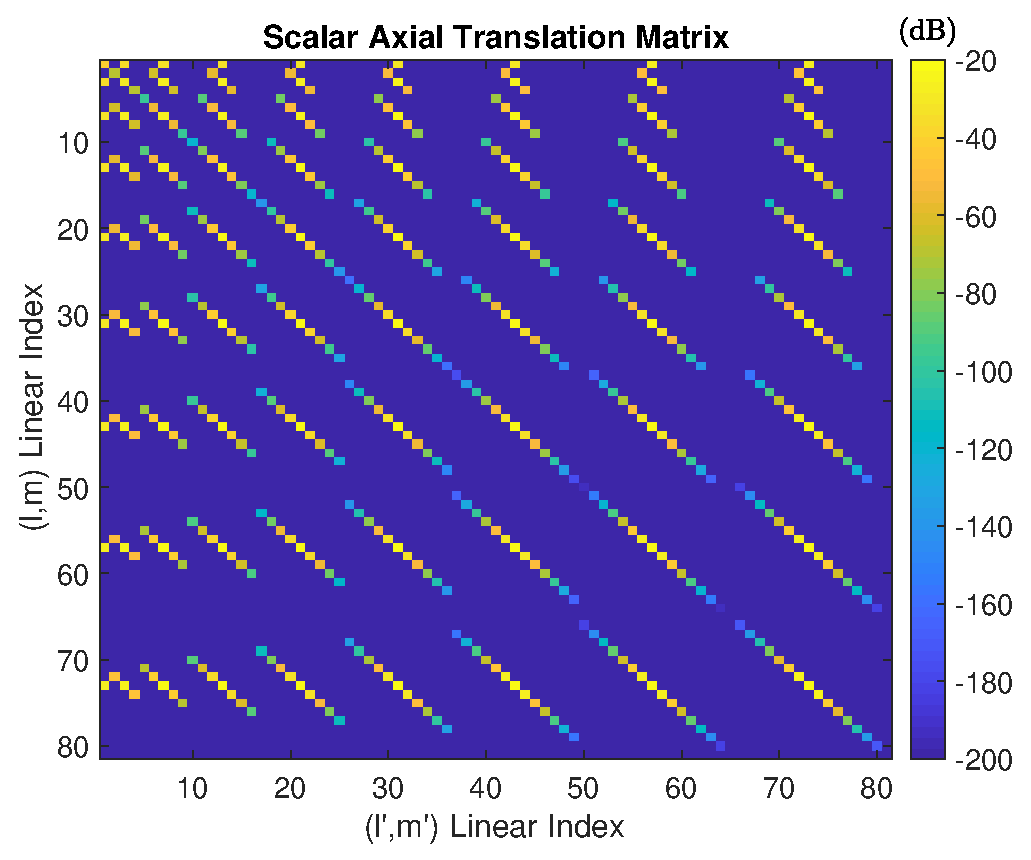
\includegraphics[width=3.5in]{Translation/Figures/trans1} 
   \caption{Scalar axial translation matrix, $L = L' = 8$, $k = 1$, $r_{ji} = 100$. }
   \label{fig4}
\end{figure}



The routine \texttt{alphaz} takes as input the largest row degree, $L$, the largest column degree $L'$, wavenumber $k$, axial translation distance $r_{ji}$, and returns the translation matrix in full, including zeros.  Use string switch \texttt{'rg'} for the regular form. This routine is a good starting point for visualization, but the output matrix should not be used as is for matrix-vector multiplication due to the zeros, or it should be converted to a sparse matrix. The routine is written with the variable $n$ in place of $l'$ for clarity. 

{\footnotesize
\VerbatimInput{\code/Translation/alphaz.m}
}


\clearpage
\subsection{Sparse Scalar Axial Translation Matrix}

We want to compute the inherently sparse axial translation matrix on a 1D array, to avoid preallocating a potentially massive, mostly zero, matrix. Indexing is more complicated than for the sparse rotation matrix due to different sized diagonal subblocks as well as the triangular fill region requirement. Analytic formulas for sparse indexing are derived and used below. As implemented, these add a little computation time relative to indexing on the full preallocated matrix. 

\begin{figure}[H] 
  \centering
 \includegraphics[width=5.5in]{Translation/Figures/sparseindex_2} 
   \caption{Indexing the diagonal subblocks of the sparse scalar axial translation matrix. Blue arrows indicate the direction of the linear indexing.  }
   \label{fig2translation}
\end{figure}


The total number of non-zero matrix elements in the scalar axial translation matrix, but not including the required triangular fill region, is counted as 
\begin{eqnarray}
N(L,L') &=& \sum_{l' = 0}^{L'} \sum_{l=0}^{L} \sum_{m = -\textrm{min}(l,l')}^{\textrm{min}(l,l')} 1 \label{eq:NLL}\\
\ & = & \sum_{l' = 0}^{L'} \sum_{l=0}^{L} \left( \textrm{2 min}(l,l') + 1 \right) \label{crazysparse}
\end{eqnarray}  

This counts the total number of elements in a matrix that has $L \times L'$ subblocks. The number of non-zero elements along the diagonal of a subblock is determined by the smaller of the $l$ and $l'$. See Figure \ref{fig2translation}.  Plugging \eqref{crazysparse} into Wolfram Alpha we get
\begin{equation}
N(L,L') 
= \left\{
\begin{array}{ccc}
1 & \ & L =  L' = 0 \\
L'+1 &\ & L = 0, L' >0\\
L + 1 & \ & L' = 0 , L>0\\
-L'^3/3+L'^2 L+L' (2 L+4/3)+L+1 & \ & L'<L, L>0,L'>0 \\
-L^3/3+L^2 L'+L (2 L'+4/3)+L'+1 & \ & L'>L, L>0,L'>0 \\
2/3L^3 + 2L^2 + 7/3L + 1 & \ & L' = L, L>0,L'>0 \\
\end{array}
\right.
 \label{eq:a1}
\end{equation}

Next, the total number of nonzero elements in the triangular fill region, see Figure \ref{fig2translation2}, assuming $L \ge L'$, and assuming that the original matrix is extend along rows, is given by 
\begin{equation}
N_{\textrm{fill}}(L,L') = \sum_{l' = 0}^{L'-1} \sum_{l=L+1}^{L + L' - l'} \left( 2 l' + 1 \right) = L'(2L'^2 + 3L' + 1)/6  \label{eq:a2}\end{equation}



\begin{figure}[H] 
   \centering
      \includegraphics[width=3.5in]{Translation/Figures/sparseindex_3} 
   \caption{Indexing the diagonal subblocks of the triangular fill region of the sparse scalar axial translation matrix. Blue arrows indicate the direction of the linear indexing. }
   \label{fig2translation2}
\end{figure}


Because we have defined the fill region as additional matrix rows, the 1D crop is easiest if we index the diagonal $(l,l')$ subblocks as "row"-major (left-right, top-down), and where we index the diagonals of the subblocks from upper left to lower right. See again Figure \ref{fig2translation}. Once the computation is complete we keep the first $N(L,L')$ elements and apply the transpose if $L' > L$.  

The "row"-major 1D linear index for the axial translation matrix, but not including the triangular fill region, is given by  
\begin{equation}
I(l,l',m,L') = N(l-1,L') + \sum_{i = 0}^{l'-1}  (2\textrm{min}(l,i) + 1)  + (\textrm{min}(l,l') + m + 1)   \label{eq:a3}
\end{equation}

\noindent where
\begin{equation}
\sum_{i = 0}^{l'-1}  (2\textrm{min}(l,i) + 1) = 
\left\{\begin{array}{cc} 
l'^2, & l' = 1 \lor ( l+1>l' \land l' > 1) \\
-l^2 - l + 2ll' + l' & \textrm{otherwise} \\
\end{array}
\right\}
\end{equation}  

$N(l-1,L')$ counts the submatrix containing all diagonal subblocks up to but not including the desired $l$ row of diagonal blocks. The second term counts completed column blocks in the current row block up that go up to but do not include the desired $l'$. The last term counts the desired diagonal. This counting requires knowledge of $L'$.

Finally, the linear index of an element in the triangular fill region under the conditions that $L \ge L'$, $l > L$, and $0 \le l' \le L'-1$ is
\begin{eqnarray}
I_{\textrm{fill}}(l,l',m,L,L') &=& N(L,L') + \sum_{i= L+1}^{l-1} \left(\sum_{j=0}^{L'-1-(i-L-1)}(2j+1)\right) \nonumber \\
\ & \ & + \left(\sum_{j=0}^{l'-1} (2j + 1)\right) + (l' + m + 1)  \label{eq:a4} \\
\ & =& N(L,L') + \left( 1/6(l-L-1)(2l^2-l(4L+6Lp+7)+2L^2\right. \nonumber \\
\ & \ & \left. +L(6Lp+7)+6(Lp+1)^2)\right) + l'^2 + (l' + m + 1) 
\end{eqnarray}

The first term counts the number of elements in the actual matrix.  The second term counts the completed row blocks up to but not including the current row block in the fill triangle.  The third term counts the column blocks in the current row block to go up to but do not include the active diagonal (this is made simpler by the fact that $l' < l$ in the fill region).  The last term indexes the active diagonal.  



The routine \texttt{alphazSparse} returns three column arrays of the row index, column index, and matrix entries of the sparse axial translation matrix.  It is the same as \texttt{alphaz} but computed and output on a 1D array. Helper functions are given in Table \ref{sparsetranshelp}. \texttt{Nalphaz} and \texttt{Nalphazfill} count the number of nonzero elements in the matrix and fill region, respectively. \texttt{indAlphazFill} is used to index the sparse matrix including the fill regions; it calls \texttt{indAlphaz} which indexes the primary sparse matrix.  When $L' > L$, the transpose is accomplished by applying \eqref{azflip} and reordering row, column, and array elements to be consistent with the row-major indexing of \texttt{indAlphaz}.  


\begin{table}[htbp]
\caption{\texttt{alphazSparse} Helper Functions}
\begin{center}
\begin{tabular}{|c|c|c|}
\hline
Routine & Equation & Description \\
\hline
\texttt{Nalphaz} &   \eqref{eq:a1} & Number of non-zero elements in $L \times L'$ sparse $\alpha_{lm,l'm'}$ \\
\hline
\texttt{Nalphazfill} &  \eqref{eq:a2} & Number of non-zero elements in fill region \\
\hline
\texttt{indAlphaz} &   \eqref{eq:a3} & Row-major 1D linear index in sparse $\alpha_{lm,l'm'}$ \\
\hline
\texttt{indAlphazFill} &  \eqref{eq:a4} & Row-major 1D linear index in sparse fill region \\ 
\hline
\end{tabular}
\end{center}
\label{sparsetranshelp}
\end{table}%


{\footnotesize
\VerbatimInput{\code/Translation/alphazSparse.m}
}

{\footnotesize
\VerbatimInput{\code/Translation/Nalphaz.m}
}

{\footnotesize
\VerbatimInput{\code/Translation/Nalphazfill.m}
}

{\footnotesize
\VerbatimInput{\code/Translation/indAlphaz.m}
}

{\footnotesize
\VerbatimInput{\code/Translation/indAlphazFill.m}
}


\clearpage
\subsection{Diagonalized Scalar Translation Matrix}

After creating sparse rotation and axial translation matrices, the matrix-vector multiplication should be carried out right to left in sequence otherwise the benefit of diagonalization is lost. For example, if \texttt{a} is a vector of expansion coefficients, and the matrices are in Matlab's sparse matrix format, then the multiplication should be carried out as follows \texttt{b = conj(D)*(Alphaz*(D*a))}.

The routine \texttt{scalarTranslation} takes as input a vector of expansion coefficients in frame $i$, $\bb{a}$, the maximum degrees $L$ and $L'$ of the translation matrix and the translation vector $\br_{ji}$ and returns expansion coefficients in frame $j$, $\bb{b}$. The length of $\bb{a}$ should be $L'^2 + 2L' + 1$.  Use \texttt{'rg'} for the regular form of the translation.  This uses the routines for the sparse forms of the rotation matrix and axial translation matrix to save memory. If the entire matrix is desired then include the optional second output. 


{\footnotesize
\VerbatimInput{\code/Translation/scalarTranslation.m}
}

\clearpage
\subsection{Full Scalar Translation Matrix}

Recursion relations to compute the full scalar translation matrix were derived in \cite{chew1992recurrence}. While diagonalization is efficient for large matrices, using the full-matrix recursion is more efficient when the number of rows or columns in the matrix are small. The sums of the additional theorem are technically infinite, however, if the field being translated is known to have low harmonic content, then there is no need to compute the matrix beyond the maximum harmonic. For example, the field expansion of a pure scalar dipole only contains harmonics up to degree $l = 1$ (i.e., $(l,m)$ = (0,0),(1,-1),(1,0),(1,1)). Translating this field as incoming waves in the frame of a large scattering object requires only four matrix columns, but a large number rows. The same computation done with diagonalization needs a square rotation matrix to match the number of harmonics of the rows, which is more computation than necessary. Finally, being able to compute the full matrix is useful for cross checking. 


\begin{figure}[H] 
\centering
   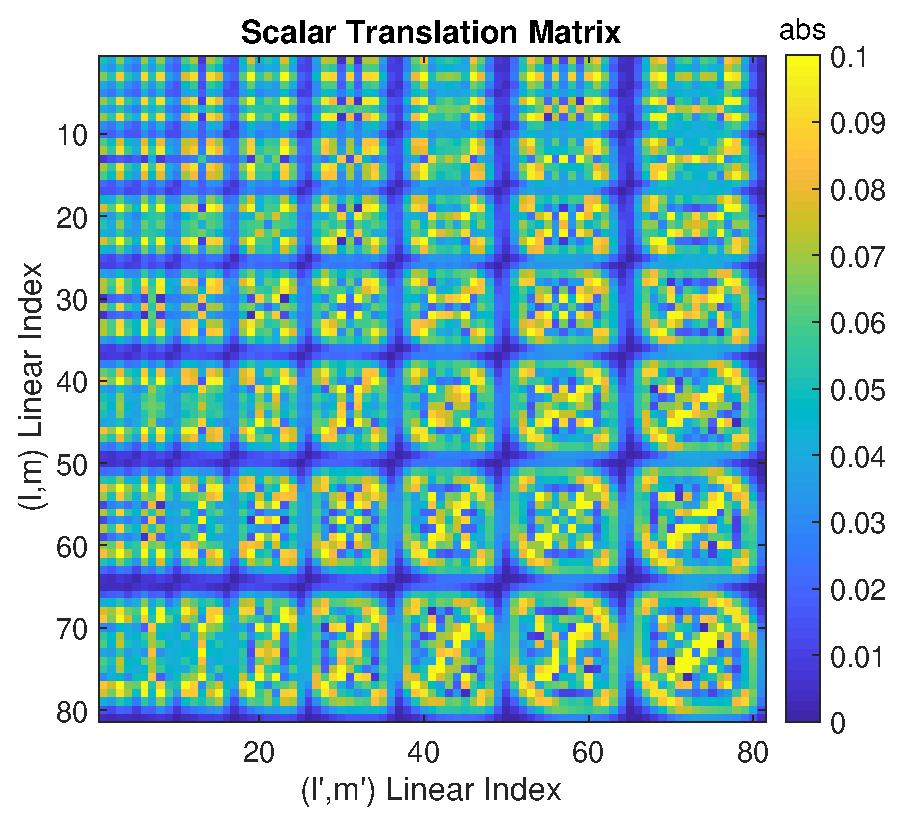
\includegraphics[width=3.5in]{Translation/Figures/transfull} 
   \caption{Scalar translation matrix, $L = L' = 8$, $k = 1$, $r_{ji} = [12, 5, 15]$.} 
\end{figure}


Adopting the notation from \cite{chew1992recurrence}, which uses the pairings $(\nu\mu,nm)$ for our $(lm,l'm')$, the recurrence relations for the full scalar translation matrix are initialized with
\eq{\alpha_{\nu\mu,00} = \sqrt{4\pi} (-1)^{\nu}Y^*_{\nu\mu}(\theta,\phi)h_{\nu}^{(1)}(k r)}

\noindent where $(r,\theta,\phi)$ are the spherical coordinates of the vector, $\br_{ji}$, that points from the originating frame to the translated frame. The first recursion relation is
\eq{b_{nn}^{+} \alpha_{\nu\mu,n+1,n+1} = b_{\nu-1,\mu-1}^{+} \alpha_{\nu-1,\mu-1,nn}  + b_{\nu+1,\mu-1}^{-} \alpha_{\nu+1,\mu-1,nn}}

This is also used to iterated on $b_{n,-n}^{+} \alpha_{\nu\mu,n+1,-(n+1)} $. The second relation is 
\eq{a_{nm}^{+} \alpha_{\nu\mu,n+1,m}  = -a_{nm}^{-} \alpha_{\nu\mu,n-1,m} + a_{\nu-1,\mu}^{+} \alpha_{\nu-1,\mu,nm} + a_{\nu+1,\mu}^{-} \alpha_{\nu+1,\mu,nm} }

The coefficients are 
\ea{a_{nm}^{+} &=& -\sqrt{ \dfrac{(n+m+1)(n-m+1)}{(2 n+1)(2 n+3)}} \\
a_{nm}^{-} &=& \sqrt{\dfrac{(n+m)(n-m)}{(2n+1)(2n-1)}} }
\ea{b_{nm}^{+} &=& \sqrt{\dfrac{(n+m+2)(n+m+1)}{(2n+1)(2n+3)}} \\
b_{nm}^{-} &=& \sqrt{\dfrac{(n-m)(n-m-1)}{(2n+1)(2n-1)} }}
Like the axial translation matrix, the computation requires a triangular fill region. As before, the fill region is placed along the dimension of the matrix with the highest degree harmonic, because we only need to fill to the smaller of $L$ and $L'$. We always fill along rows, so if the matrix needs to be flipped, the following transpose relation is used
\eq{\alpha_{mn,\nu\mu} = (-1)^{\nu+\mu+m+n} \alpha_{\nu,-\mu,n,-m}}
   
The routine \texttt{alpha} computes the full scalar translation matrix using the recursion relations above.  It takes as input the largest row degree, $L$, the largest column degree $L'$, wavenumber $k$, axial translation vector $\br_{ji}$, and returns the translation matrix linearly indexed along rows and columns. Use string switch \texttt{'rg'} for the regular form. The computation fills along rows for the larger of $L$ and $L'$, then transposes the matrix if necessary. This routine matches the outputs of the diagonalized version to machine precision. 


{\footnotesize
\VerbatimInput{\code/Translation/alpha.m}
}



\clearpage
\newpage

\section{Vector Translation Matrix}

This section gives routines for the vector axial translation matrix, sparse vector axial translation matrix, and an implementation of the diagonalized matrix-vector multiplication.  
\vspace{-1mm}
\subsection{Vector Axial Translation Matrix}

The vector axial translation matrices are found directly from the scalar axial translation matrix with the following relations:
\begin{eqnarray}
A_{l,m,l',m} &=& k r_{ji}\left[\dfrac{1}{(l+1)}\sqrt{\dfrac{(l+m+1)(l-m+1)}{(2l+3)(2l+1)}} \alpha_{l+1,m,l',m} \right. \nonumber \\
\ & \ & + \left. \dfrac{1}{l}\sqrt{\dfrac{(l+m)(l-m)}{(2l+1)(2l-1)}}\alpha_{l-1,m,l',m} \right] + \alpha_{l,m,l',m} \\
B_{l,m,l',m} &=& \dfrac{imkr_{ji}}{l(l+1)}\alpha_{l,m,l',m} 
\end{eqnarray}
\begin{equation}
A_{l,m,l',m'} = B_{l,m,l',m'} = \alpha_{l,m,l',m'} = 0, \quad \quad m \ne m'
\end{equation}

Because the first equation uses $l+1$, the scalar axial matrix needs one extra degree $l = L+1$.  The equations in \cite{mackowski1991analysis} appear to be missing several scaling factors, but \cite{chew1993efficient} gives correct equations.  Both \cite{mackowski1991analysis, chew1993efficient} derived translation matrices for partially normalized vector spherical waves functions.  For fully normalized vector spherical wave functions, the vector translation matrices need to be modified as 
\begin{eqnarray}
\widetilde{A}_{l,m,l',m'} &=& \sqrt{\dfrac{l(l+1)}{l'(l'+1)}} A_{l,m,l',m'}\\
\widetilde{B}_{l,m,l',m'} &=& \sqrt{\dfrac{l(l+1)}{l'(l'+1)}}B_{l,m,l',m'}
\end{eqnarray}

The routine \texttt{AzBz} takes as input the maximum harmonic degrees $L$ and $L'$, wavenumber $k$, and magnitude of the z-axis translation, $r_{ji}$, and returns vector translation matrices $A_{l,m,l',m}$ and $B_{l,m,l',m}$. Use string switch \texttt{'rg'} for the regular form of the matrices, and \texttt{'norm'} for fully normalized vector wave functions. 

{\footnotesize
\VerbatimInput{\code/Translation/AzBz.m}
}




\subsection{Sparse Vector Axial Translation Matrix}

Because the vector axial translation matrices are computed directly from the scalar functions, they are sparse and can be computed on a 1D array.  We only need to count the number of elements in the vector axial translation matrix and determine its sparse linear index. The number of elements in the sparse vector axial translation matrix is counted the same as the scalar case starting at $l=1$ and $l'=1$.  
\begin{eqnarray}
N(L,L') &=& \sum_{l' = 1}^{L'} \sum_{l=1}^{L} \sum_{m = -\textrm{min}(l,l')}^{\textrm{min}(l,l')} 1 \label{eq:NLL}\\
\ & = & \sum_{l' = 1}^{L'} \sum_{l=1}^{L} \left[ 2 \textrm{min}(l,l') + 1 \right]
\end{eqnarray}  

Plugging this into Wolfram Alpha
\begin{equation}
N(L,L') 
= \left\{
\begin{array}{ccc}
3 & \ & L =  L' = 1 \\
3L &\ & L' = 1, L >1\\
3L' & \ & L = 1 , L' >1\\
- 1/3L'^3  + L L'^2 + 2 LL' + 1/3L' & \ & L > 1, L' > 1, L > L'\\
-1/3L^3  + L'L^2 + 2L'L + 1/3L& \ &  L > 1, L' > 1, L'>L \\
L^2 + 5L + 2/3L'^3 + L'^2 - 14/3L' & \ & L > 1, L' > 1, L = L' \\
\end{array}
\right.
\end{equation}

Counting row-major, the sparse linear index is 
\begin{equation}
I(l,l',m,L') = N(l-1,L') + \sum_{i = 1}^{l'-1}  (2\textrm{min}(l,i) + 1)  + (\textrm{min}(l,l') + m + 1)  
\end{equation}

\noindent where
\begin{equation}
\sum_{i = 1}^{l'-1}  (2\textrm{min}(l,i) + 1) = 
\left\{\begin{array}{ccc} 
3 & \ & l + 1 \ge l' \land ((l=1 \land l' \ge 2) \lor (l' = 2 \land l > 1 )) \\
2l(l'-2) + l' + 1 & \ & l + 1 < l' \land ((l=1 \land l' \ge 2) \lor (l' = 2 \land l > 1 )) \\
l'^2 - 1  & \ & l > 1 \land l+1 \ge l' \land l > 2 \\
-l^2 + l + (2l + 1)(l'-1)& \ & \textrm{otherwise} \\
\end{array}
\right\}
\end{equation}  


The routine \texttt{AzBzSparse} returns four column arrays of the row index, column index, and matrix entries of the sparse axial translation matrices.  It is the same as \texttt{AzBz} but computed and output on a 1D array.  The helper functions are \texttt{NAzBz.m} and \texttt{indAzBz.m}.


{\scriptsize
\VerbatimInput{\code/Translation/AzBzSparse.m}
}

{\scriptsize
\VerbatimInput{\code/Translation/NAzBz.m}
}

{\scriptsize
\VerbatimInput{\code/Translation/indAzBz.m}
}

\clearpage
\subsection{Diagonalized Vector Translation Matrix}


The routine \texttt{vectorTranslation} takes as input a vector of expansion coefficients in frame $i$, $\bb{a}$ and $\bb{b}$, the maximum degrees $L$ and $L'$ of the translation matrix and the translation vector $\br_{ji}$ in Cartesian coordinates and returns expansion coefficients in frame $j$, $\bb{c}$ and $\bb{d}$. The lengths of $\bb{a}$ and $\bb{b}$ should be $L'^2 + 2L' $.  Use \texttt{'rg'} for the regular form and \texttt{'norm'} for fully normalized vector wave functions. This uses the routines for the sparse versions of the rotation matrix and axial translation matrices to save memory.  If the pair of matrices is desired, then include the optional third and fourth outputs. 


{\scriptsize
\VerbatimInput{\code/Translation/vectorTranslation.m}
}
\clearpage

\subsection{Full Vector Translation Matrix}

Like the full scalar translation matrix, recursion relations to compute the full vector translation matrices were derived in \cite{chew1993efficient}. Two versions are available: the first iterates on the vector matrices from scratch, the second iterates on the full scalar translation matrix. We implement the second version, which requires computing the scalar translation matrix at a maximum harmonic degree one higher than that of the vector matrices. 


\begin{figure}[H] 
   \centering
   \subfigure{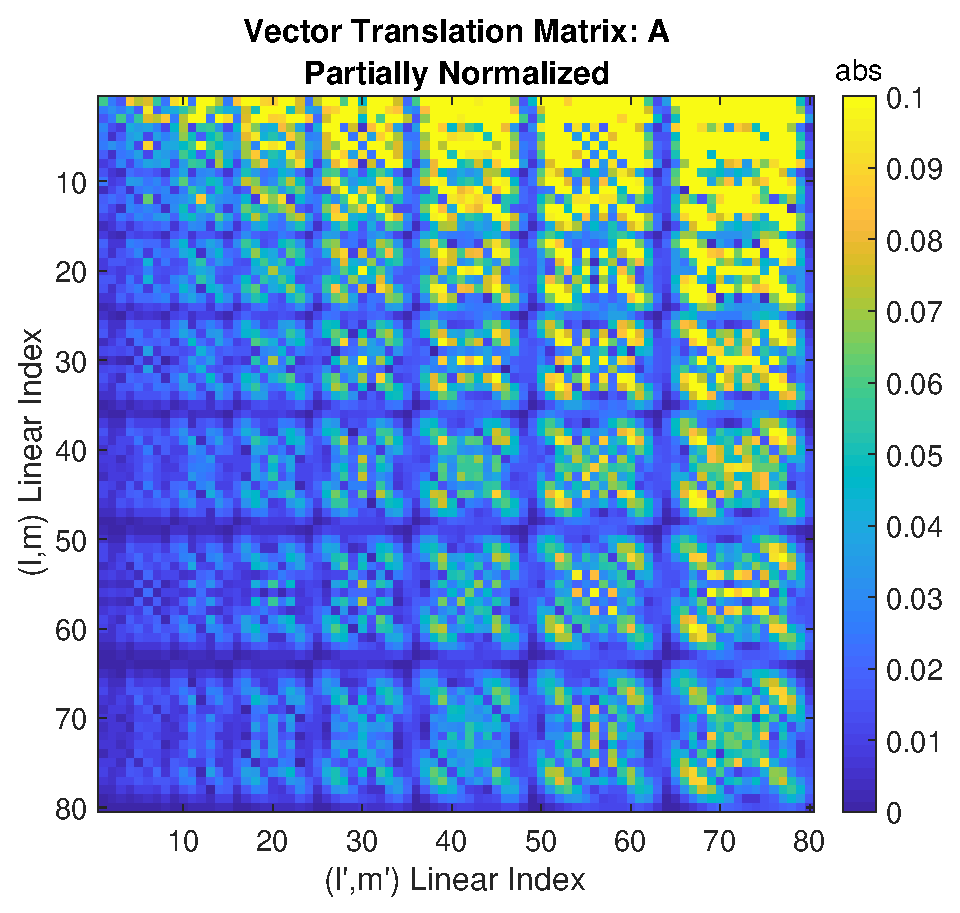
\includegraphics[width=3in]{Translation/Figures/transfullA1}}
   \subfigure{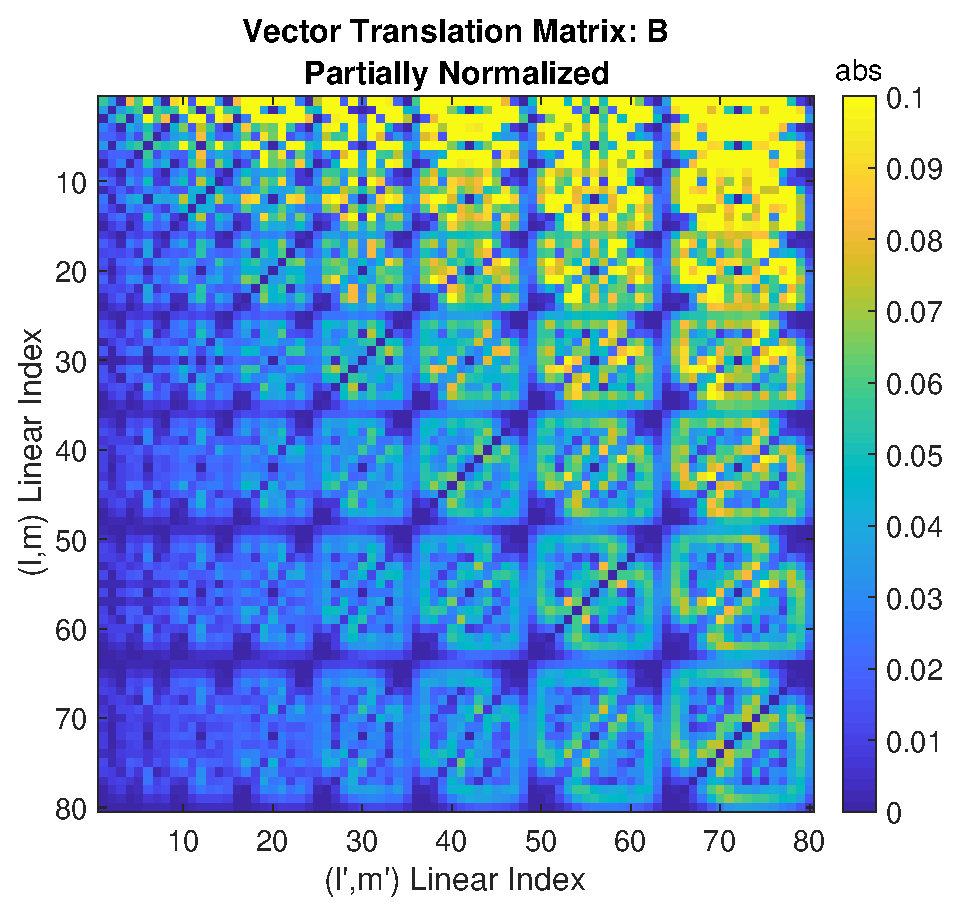
\includegraphics[width=3in]{Translation/Figures/transfullB1}} \\
   \subfigure{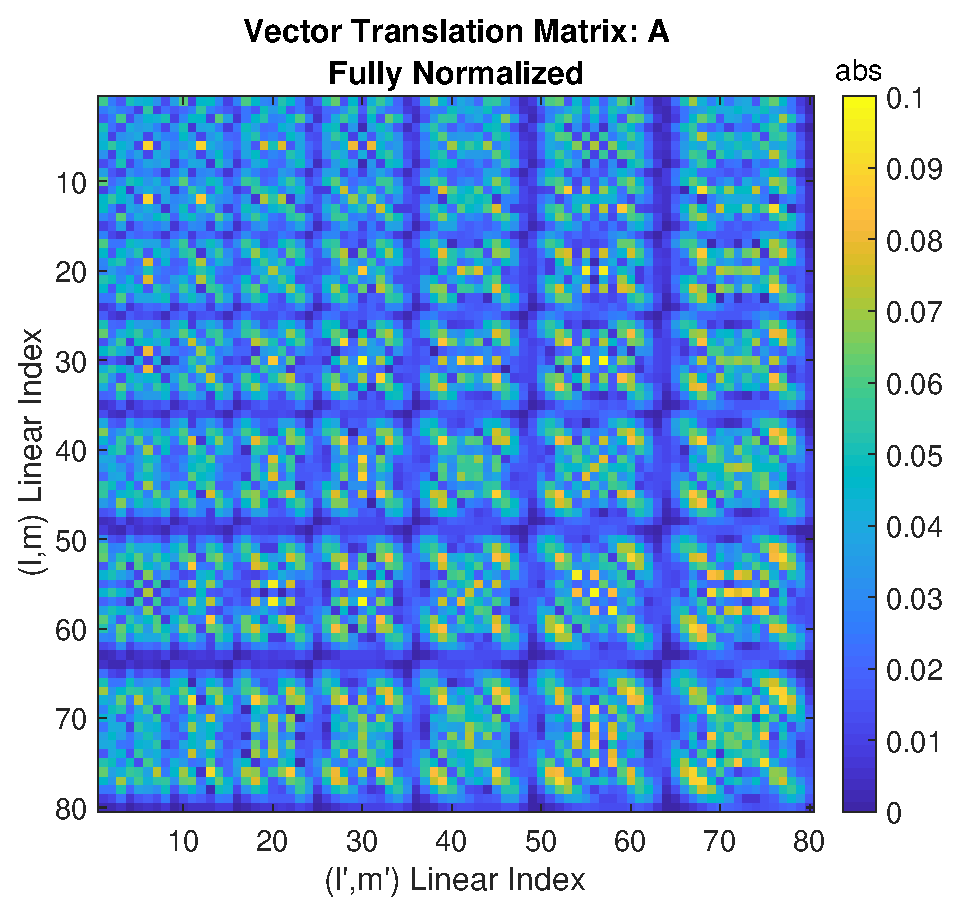
\includegraphics[width=3in]{Translation/Figures/transfullA2}}
   \subfigure{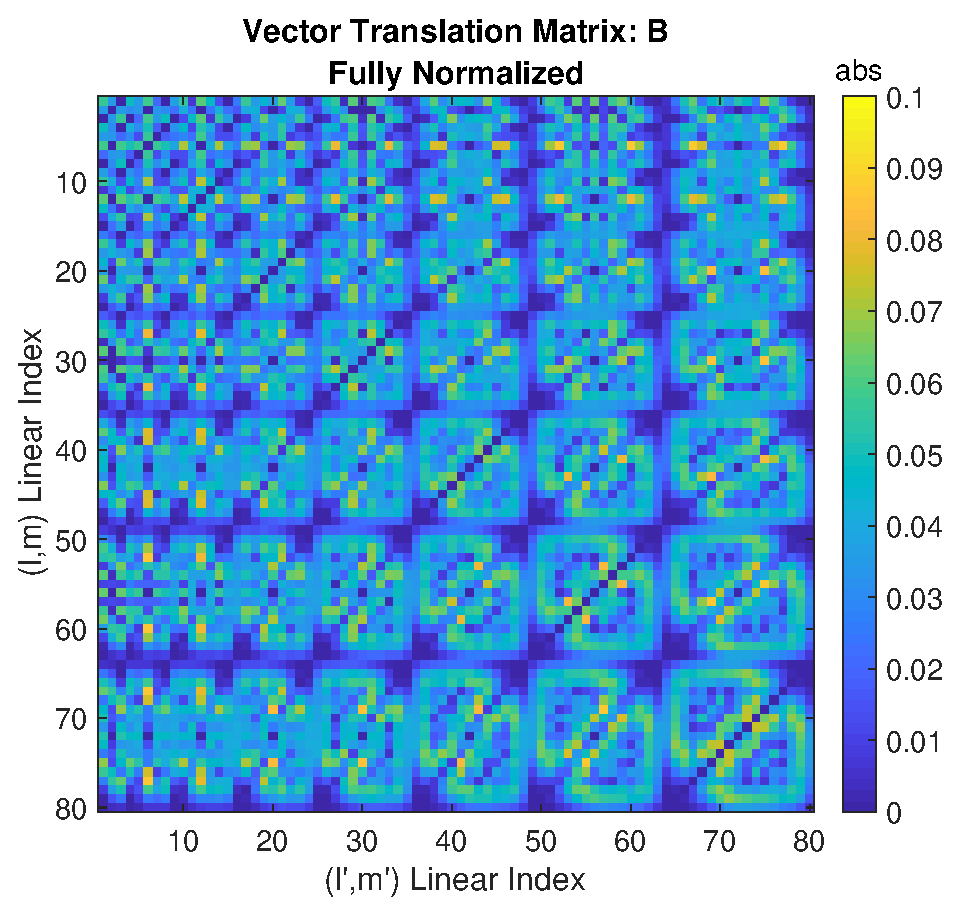
\includegraphics[width=3in]{Translation/Figures/transfullB2}}
   \caption{Vector translation matrices for $L = L' = 8$, $k = 1$, $r_{ji} = [12, 5, 15]$. Top row: matrices for partially normalized vector wave functions. Bottom row: matrices for fully normalized vector wave functions.}
   \label{transfullAB}
\end{figure}


Adopting the notation from \cite{chew1993efficient}, which uses the pairings $(\nu\mu,nm)$ for our $(lm,l'm')$, the recurrence relations for the two vector translation matrices derived from the scalar translation matrix are
\ea{A_{\nu\mu,nm} &=& \alpha_{\nu\mu,nm} + 
c_{1,\nu\mu} \alpha_{\nu+1,\mu-1,nm} + 
c_{2,\nu\mu} \alpha_{\nu-1,\mu-1,nm} + 
c_{3,\nu\mu} \alpha_{\nu+1,\mu+1,nm} + \nonumber \\
\ & \ & 
c_{4,\nu\mu} \alpha_{\nu-1,\mu+1,nm} + 
c_{5,\nu\mu} \alpha_{\nu+1,\mu,nm} + 
c_{6,\nu\mu} \alpha_{\nu-1,\mu,nm} 
\label{Anumu} \\
B_{\nu\mu,nm} &=& c_{7,\nu\mu} \alpha_{\nu\mu,nm} + 
c_{8,\nu\mu} \alpha_{\nu,\mu+1,nm} + 
c_{9,\nu\mu} \alpha_{\nu,\mu-1,nm} \label{Bnumu} } 

Note, \eqref{Anumu} and \eqref{Bnumu} only operate on the row indices $(\nu,\mu)$. The coefficients are 
\ea{
c_{1,\nu\mu} &=& \dfrac{kr\sin\theta e^{-i\phi}}{2(\nu + 1)}\sqrt{\dfrac{(\nu-\mu+2)(\nu-\mu+1)}{(2\nu + 1)(2\nu + 3)}} \\
c_{2,\nu\mu} &=&  -\dfrac{kr\sin\theta e^{-i\phi}}{2\nu}\sqrt{\dfrac{(\nu+\mu-1)(\nu+\mu)}{(2\nu - 1)(2\nu + 1)}} \\
c_{3,\nu\mu} &=& -\dfrac{kr\sin\theta e^{i\phi}}{2(\nu + 1)}\sqrt{\dfrac{(\nu+\mu+2)(\nu+\mu+1)}{(2\nu + 1)(2\nu + 3)}} \\
c_{4,\nu\mu} &=&  \dfrac{kr\sin\theta e^{i\phi}}{2\nu}\sqrt{\dfrac{(\nu-\mu)(\nu-\mu-1)}{(2\nu - 1)(2\nu + 1)}}\\
c_{5,\nu\mu} &=& \dfrac{kr\cos\theta}{\nu+1}\sqrt{\dfrac{(\nu+\mu+1)(\nu-\mu+1)}{(2\nu + 1)(2\nu + 3)}} \\
c_{6,\nu\mu} &=&  \dfrac{kr\cos\theta}{\nu}\sqrt{\dfrac{(\nu+\mu)(\nu-\mu)}{(2\nu - 1)(2\nu + 1)}}  \\
c_{7,\nu\mu} &=& \dfrac{i\mu kr\cos\theta }{\nu(\nu+1)} \\
c_{8,\nu\mu} &=& \dfrac{i kr\sin\theta e^{i\phi} }{2\nu(\nu+1)} \sqrt{(\nu-\mu)(\nu+\mu+1)} \\
c_{9,\nu\mu} &=& \dfrac{i kr\sin\theta e^{-i\phi} }{2\nu(\nu+1)} \sqrt{(\nu+\mu)(\nu-\mu+1)}  } 

\noindent where $(r,\theta,\phi)$ are the spherical coordinates of the vector $\br_{ji}$ that points from the originating frame to the translated frame.


The routine \texttt{AB} takes as input the maximum harmonic degrees $L$ and $L'$, wavenumber $k$, and translation vector, $r_{ji}$, and returns full vector translation matrices $A$ and $B$. It calls \texttt{alpha} to compute the full scalar translation matrix. Use string switch \texttt{'rg'} for the regular form of the matrices, and \texttt{'norm'} for fully normalized vector wave functions. 



{\footnotesize
\VerbatimInput{\code/Translation/AB.m}
}






\chapter{S-Matrix}
\label{chap:smatrix}

The scattering matrix, or S-matrix (also called the scattering function matrix, \cite{tsang2000scattering}), embeds the scattering behavior of an object as a mapping between incident and scattered plane-waves. It transforms between the incident/scattered directions as well as incident/scattered polarizations. This chapter gives the basic definition of the S-matrix, its relation to radar cross sections, routines for the S-matrix of simple objects, and the derivation of an object S-matrix under the Born approximation. 

\section{Definition}

From \cite{tsang2000scattering}, let an incident wave be a plane wave with wave vector $\bb{k}_i$, the polarization of which is decomposed into two linearly independent vectors that are perpendicular to $\hat{k}_i$, as
\begin{equation}
\bb{E}_i = \left( E_{pi} \hat{p}_i+  E_{qi}\hat{q}_i\right) e^{i\bb{k}_i \cdot \br}
\end{equation}

\noindent where $\bb{r}$ is the position vector, ${\bb{k}}_i = k\hat{{k}}_i$ and $\hat{p}_i$, $\hat{q}_i$ and $\hat{{k}}_i$ form an orthonormal system.  The scattered field is then defined 
\begin{equation}
\bb{E}_s = \left( E_{ps}\hat{p}_s +  E_{qs}\hat{q}_s\right) \dfrac{ e^{i k r}}{r}
\end{equation}

\noindent where the scattered field polarization vectors $\hat{p}_s$ and $\hat{q}_s$ form a right-handed orthonormal system with the scattered field direction $\hat{{k}}_s$. The scattered field components are linearly related to the incident components through the scattering matrix, or S-matrix, 
\begin{equation}
\twobyone{E_{ps}(\hat{k}_s)}{E_{qs}(\hat{k}_s)} = \twobytwo{S_{pp}(\hat{k}_s,\hat{k}_i)   }{S_{pq}(\hat{k}_s,\hat{k}_i) }{S_{qp}(\hat{k}_s,\hat{k}_i) }{S_{qq}(\hat{k}_s,\hat{k}_i) }   \twobyone{E_{pi}(\hat{k}_i)}{E_{qi}(\hat{k}_i)} 
\end{equation}
 
These definitions for the fields and S-matrix give them the following units: the incident field amplitudes $E_{pi}$ and $E_{qi}$ have units of electric field (V/m), the S-matrix elements have units of length (m), and the scattering field amplitudes $E_{ps}$ and $E_{qs}$ have units of (Vm/m = V) because the length dimension of the factor of $1/r$ needs to be included. This depends on convention, because some definitions of the S-matrix use $1/kr$ outside the S-matrix, which makes the S-matrix unitless. 

We use the wave vector and polarization convention of \cite{tsang2000scattering}. The polarizations are taken as $\hat{p} = \hat{v}$ and $\hat{q} = \hat{h}$ with wave vector directions
\ea{\hat{k}_i &=&  \sin\theta_i \cos\phi_i \hat{x}  + \sin\theta_i \sin\phi_i \hat{y} + \cos\theta_i \hat{z} \label{khati} \\
\hat{v}_i &=& \cos\theta_i \cos\phi_i \hat{x} + \cos\theta_i\sin\phi_i \hat{y} - \sin\theta_i\hat{z} \\
\hat{h}_i &=& -\sin\phi_i\hat{x} + \cos\phi_i \hat{y} \\
\hat{k}_s &=& \sin\theta_s \cos\phi_s \hat{x}  + \sin\theta_s \sin\phi_s \hat{y} + \cos\theta_s \hat{z} \label{ss1} \\
\hat{v}_s &=& \cos\theta_s \cos\phi_s \hat{x} + \cos\theta_s\sin\phi_s \hat{y} - \sin\theta_s\hat{z} \\
\hat{h}_s &=& -\sin\phi_s\hat{x} + \cos\phi_s \hat{y} \label{hhats}}

\noindent where $\theta$, $\phi$ are spherical directions of the propagation waves. Here, the wave vectors are treated as radial vectors, and $\hat{v}$ and $\hat{h}$ are equivalent to the $\hat{\theta}$ and $\hat{\phi}$ spherical unit vectors. The polarizations for $\hat{z}$ propagating waves ($\theta = 0$ or $\theta = \pi$) are well-defined by using $\phi=0$ as a reference
 \ea{\hat{k}(0,0) &=&  \hat{z} \\
\hat{v}(0,0) &=& \hat{x} \\
\hat{h}(0,0) &=& \hat{y} \\
\hat{k}(\pi,0) &=&  -\hat{z} \\
\hat{v}(\pi,0) &=& -\hat{x}  \\
\hat{h}(\pi,0) &=& - \hat{y} }

These special cases can be used as definitions of the $\hat{\theta}$ and $\hat{\phi}$ unit vectors at the poles.

\section{Radar Cross Sections from S-matrix}

We list different radar cross sections and their relations to the S-matrix. Most of these can be found in \cite{tsang2000scattering}.

\paragraph{Radar Cross Section} The bistatic radar cross section is defined 
\ea{\sigma_{pq}(\hat{k}_s,\hat{k}_i) &=& \lim_{r \rightarrow \infty} 4\pi r^2 \dfrac{\left\vert \hat{p} \cdot \bb{E}_s \right\vert^2}{\left\vert \hat{q} \cdot \bb{E}_i \right\vert^2} \\
\ &=& 4\pi \vert S_{pq} \vert^2 \label{rcsfromSpq} }

\noindent where $p$ and $q$ are any two orthogonal polarizations. The units of radar cross section are area or length-squared, showing again that $S_{pq}$ has units of length.

\paragraph{Scattering Cross Section} The total scattering cross section for incident direction $\hat{k}_i$ and arbitrary incident polarization $\hat{\beta}$, such that $\hat{\beta} \cdot \hat{k}_i = 0$, is computed as the integral over scattered field directions $\hat{k}_s$ as
\eq{\sigma_{s\beta}(\hat{k}_i) = \int \left( \vert S_{p\beta}(\hat{k}_s,\hat{k}_i) \vert^2 + \vert S_{q\beta}(\hat{k}_s,\hat{k}_i) \vert^2 \right) d\Omega_s }

\noindent where
\eq{
\twobyone{S_{p\beta}  }{S_{q\beta}  } = 
\twobytwo{S_{pp}}{S_{pq}}{S_{qp}}{S_{qq}} \twobyone{\hat{p}\cdot \hat{\beta}}{\hat{q}\cdot \hat{\beta}} \label{projectedsmatrix} 
}

\noindent and $\beta$ is the angle of the incident polarization relative to the two orthogonal polarizations of the S-matrix, which is 
\eq{\hat{\beta} = \cos\beta \hat{p} + \sin\beta \hat{q}}

\paragraph{Extinction Cross Section} The extinction cross section (or total cross section) for a given incident direction is given by the optical theorem, \cite{zhang2019generalized}, as the imaginary part of the co-polarized scattered field in the forward direction
\eq{\sigma_{ext,\beta}(\hat{k}_i) = \dfrac{4\pi}{k}\textrm{Im}\left[S_{\beta\beta}(\hat{k}_i,\hat{k}_i)\right]}

\paragraph{Absorption Cross Section} The absorption cross section is defined as the power absorbed by the scattering object divided by the power scattered. It can be written in terms of the extinction and total cross sections as 
\eq{\sigma_a = \sigma_{ext} - \sigma_s}

This subtraction is sometimes numerically inaccurate and so the absorption cross section can also be defined directly in terms of the internal field, \cite{yurkin2007discrete}.

\paragraph{Polarization and Orientation Averaged Scattering Cross Section}

The polarization and orientation averaged scattered cross section is given by the integral of the scattering cross section over all possible incident directions and polarizations including normalization:
%\eq{\left< \sigma \right> = \left<  \sigma_{s\beta}(\hat{k}_i)  \right>_{\beta,\hat{k}_i} = \dfrac{1}{2\pi} \int_0^{2\pi}\left(  \dfrac{1}{4\pi} \int \sigma_{s\beta}(\hat{k}_i) d\Omega_i \right) d\beta }
\eq{\left< \sigma \right> =  \dfrac{1}{2\pi} \int_0^{2\pi}\left(  \dfrac{1}{4\pi} \int \sigma_{s\beta}(\hat{k}_i) d\Omega_i \right) d\beta \label{polorientavescs} }

This requires projecting a given incident polarization $\beta$ onto $\hat{p}$ and $\hat{q}$, computing the projected S-matrix elements \eqref{projectedsmatrix}, computing the scattering cross section for all incident directions, then integrating over incident direction and incident angle $\beta$. Computing this does not require one to explicitly rotate or recompute the S-matrix once it is known.


\paragraph{Scattering Efficiencies} The quantities above can be reinterpreted as efficiencies by dividing by the cross sectional area of the target.  For example, the scattering efficiency for a given incident direction is given by the scattering cross section divided by cross sectional area of the target, $A$,  

\eq{Q_{sca} = \dfrac{\sigma_{s}}{A} }

The same can be applied to extinction and absorption cross sections.  

\section{S-matrix Rotation}

An S-matrix will often be computed in a reference frame aligned naturally with the geometry of the object. If an object is rotated relative to a global frame, then the incident and scattered directions and polarization in the global frame will appear to rotate in the frame of the object. It can be efficient to transform the global wave vectors and polarizations such that the S-matrix is evaluated in the frame of the object, rather than try to obtain the S-matrix of the rotated object in the global frame. Both \cite{tsang2000scattering} and \cite{van2011synthetic} give equations and procedures for rotating an object with cylindrical symmetry. We give a general procedure next.

%For the purposes of rotation, both the wave vectors and polarization vectors can be treated as Cartesian unit vectors with their tail at the origin. An extrinsic rotation is first applied to the incident and scattered directions to 
%
%The polarization vectors are then decomposed into the local $\hat{v}$ and $\hat{h}$ polarizations of the object frame. Then the S-matrix is evaluated in its frame. In this procedure, there is no need to 'rotate back', because it is sufficient to have transformed both the incident and scattered quantities to the object frame.  

Let an object rotation be described by ZXZ Euler angles $(\alpha,\beta,\gamma)$ with corresponding rotation matrix $\bb{R}$.  $\bb{R}$ describes a forward rotation, i.e., a point rides with the rotated frame. The inverse rotation is $\bb{R}^t$, where points are fixed in the global frame and we view them as though we ride with the rotating frame. The inverse rotation is first applied to the incident and scattered directions of the global frame so that they are viewed from the rotated object frame. Let these angles be $(\theta_{os},\phi_{os};\theta_{oi},\phi_{oi})$. The polarization vectors are then evaluated in the object frame at these points giving $(\hat{v}_{os},\hat{h}_{os};\hat{v}_{oi},\hat{h}_{oi})$. The object-frame polarization vectors now need to be viewed from the global frame. This is done by rotating the object-frame polarization vectors with an forward rotation, so that they appear as vectors in the global frame:
\eq{\hat{v}_{o}' = \bb{R}(\hat{v}_o)}

In matrix notation, S-matrix of the rotated object, as viewed in the global frame, is given by 
\ea{
\twobytwo{S_{vv}(\theta_s,\phi_s;\theta_i,\phi_i)}{S_{vh}(\theta_s,\phi_s;\theta_i,\phi_i)}{S_{hv}(\theta_s,\phi_s;\theta_i,\phi_i)}{S_{hh}(\theta_s,\phi_s;\theta_i,\phi_i)}
&=&
\twobytwo{\hat{v}_s \cdot \hat{v}_{os}' }{\hat{v}_s \cdot \hat{h}_{os}'}{\hat{h}_s \cdot \hat{v}_{os}'}{\hat{h}_s \cdot \hat{h}_{os}'} \cdot \nonumber \\
\ & \ & 
\twobytwo{S_{vv}(\theta_{os},\phi_{os};\theta_{oi},\phi_{oi})}{S_{vh}(\theta_{os},\phi_{os};\theta_{oi},\phi_{oi})}{S_{hv}(\theta_{os},\phi_{os};\theta_{oi},\phi_{oi})}{S_{hh}(\theta_{os},\phi_{os};\theta_{oi},\phi_{oi})} \cdot \nonumber \\
\ & \ & 
\twobytwo{\hat{v}_{oi}' \cdot \hat{v}_{i} }{\hat{v}_{oi}' \cdot \hat{h}_{i} }{\hat{h}_{oi}' \cdot \hat{v}_{i} }{\hat{h}_{oi}' \cdot \hat{h}_{i} }
} 
 
The inner matrix is the object S-matrix evaluated in its native frame using points rotated from the global frame. The outer two matrices decompose and project the polarization vectors between the two frames. 


%\subsection{Euler Rotation}

%\subsection{Cylindrical Symmetry}

\section{Object S-matrix}

\subsection{Thin Circular Cylinder}

From \cite{sarabandi1990low, stiles1996scattering} the far field scattering solution for a thin dielectric cylinder with cross sectional area much smaller than a wavelength and oriented along the $z$ axis is given by 
\eq{\bb{E}_s = -E_o\dfrac{e^{ikr}}{4\pi r} k^2 L A \left[ \hat{k}_s \times \hat{k}_s \times (\bb{P} \cdot \hat{e}_i ) \right] \sinc{(U)}}
\eq{U =  \dfrac{kL}{2} \left(\cos\theta_s - \cos\theta_i\right) }

\noindent where $L$ is the length, $A$ is the cross sectional area, $\hat{e}_i$ is the incident polarization, $k$ is the background wavenumber, $\theta_i$ and $\theta_s$ are the incident and scattered angles from the $z$ axis, and $\bb{P}$ is the polarization tensor. Also, $\textrm{sinc}(x) = \sin(x)/x$. The polarization tensor for a homogenous dielectric cylinder with circular cross section is diagonal and given by 
\ea{P_{xx} &=&  2 \dfrac{\epsilon_r - 1}{\epsilon_r + 1} \\
P_{yy} &=& 2 \dfrac{\epsilon_r - 1}{\epsilon_r + 1}\\
P_{zz} &=& \epsilon_r - 1}

\noindent where $\epsilon_r$ is the relative permittivity. For a cylinder with radius $a$, the $\hat{v}$ and $\hat{h}$ S-matrix elements are 
\ea{\twobytwo{S_{vv}}{S_{vh}}{S_{hv}}{S_{hh}} &=& \dfrac{k^2 L  a^2 }{4} \sinc{(U)} \bb{C} }

%\ea{\twobytwo{S_{vv}}{S_{vh}}{S_{hv}}{S_{hh}} &=& -\dfrac{k^2 L  a^2 }{4} \sinc{(U)} \onebytwo{\hat{v}_s}{\hat{h}_s} \cdot \twobyone{ \hat{k}_s \times \hat{k}_s \times \left(\bb{P} \cdot \hat{v}_i \right)}{ \hat{k}_s \times \hat{k}_s \times \left(\bb{P} \cdot \hat{h}_i \right) } \\
%\ &=&  \dfrac{k^2 L  a^2 }{4} \sinc{(U)} \bb{C} }

\eq{\bb{C}  = \twobytwo
{(\hat{v}_s)\cdot(\hat{k}_s \times \hat{k}_s \times \left(\bb{P} \cdot \hat{v}_i \right))}
{(\hat{v}_s)\cdot\left(\hat{k}_s \times \hat{k}_s \times \left(\bb{P} \cdot \hat{h}_i \right) \right)}
{(\hat{h}_s)\cdot(\hat{k}_s \times \hat{k}_s \times \left(\bb{P} \cdot \hat{v}_i \right))}
{(\hat{h}_s)\cdot\left(\hat{k}_s \times \hat{k}_s \times \left(\bb{P} \cdot \hat{h}_i \right) \right)} \label{matrixCforS}}

Using \eqref{khati}-\eqref{hhats} and simplifying the elements  of $\bb{C}$ are
\ea{C_{vv} &=&  P_{zz}\sin\theta_s\sin\theta_i + P_{xx}\cos\theta_s\cos\phi_s\cos\theta_i\cos\phi_i + P_{yy}\cos\theta_s\cos\theta_i\sin\phi_s\sin\phi_i \\
C_{vh} &=& \cos\theta_s(P_{yy}\sin\phi_s\cos\phi_i - P_{xx}\cos\phi_s\sin\phi_i ) \\
C_{hv} &=& \cos\theta_i(P_{yy}\cos\phi_s\sin\phi_i - P_{xx}\sin\phi_s\cos\phi_i) \\
C_{hh} &=&  P_{yy}\cos\phi_s\cos\phi_i + P_{xx}\sin\phi_s\sin\phi_i}

Applying symmetry $P_{xx} = P_{yy}$ and taking $\phi_i = 0$, these can be simplified to just
\ea{C_{vv} &=&  P_{zz}\sin\theta_s\sin\theta_i + P_{xx}\cos\theta_s\cos\phi_s\cos\theta_i \\
C_{vh} &=& P_{xx} \cos\theta_s\sin\phi_s\\
C_{hv} &=& -P_{xx} \cos\theta_i \sin\phi_s\\
C_{hh} &=&  P_{xx}\cos\phi_s}

This solution is valid for edge-on incidence, and the $hh$ and $vv$ fields become equal, which we expect.  This solution is valid for $\vert n \vert ka \ll 1$ and $a \ll L$, where $n = \sqrt{\epsilon_r}$, \cite{schiffer1979light}.

The routine \texttt{smatrix\char`_thin\char`_circular\char`_cylinder} returns the S-matrix of a thin circular cylinder. It takes the parameters of a single cylinder and computes the four block S-matrices for any number of incident and scattered directions. The block matrices have scattered directions in rows and incident directions in columns. The polarizations $\hat{v}$ and $\hat{h}$ are treated as spherical $\hat{\theta}$ and $\hat{\phi}$ in the forward scattering convention.

{\footnotesize
\VerbatimInput{\code/Smatrix/smatrix_thin_circular_cylinder.m}
}

\clearpage
\newpage

\subsection{Thin Circular Disk}

Scattering from both needles and disks is derived in \cite{schiffer1979light} and the results for needles match those in the previous section. The far field scattered field for a thin disk is
\ea{\bb{E}_s &=& -E_o\dfrac{e^{ikr}}{2\pi r} k^2 L A \left[ \hat{k}_s \times \hat{k}_s \times (\bb{P} \cdot \hat{e}_i ) \right] \textrm{jinc}(U)\\
U &=&  kL \Omega  \\
\Omega^2 &=& (\sin\theta_i \cos\phi_i- \sin\theta_s\cos\phi_s)^2 + (\sin\theta_i \sin\phi_i- \sin\theta_s\sin\phi_s )^2  }

\noindent where $L$ is the disk thickness, $A$ is cross sectional area of the disk, and $\textrm{jinc}(x) = J_1(x)/x$ where $J_1(x)$ is the Bessel function of degree 1. The polarization tensor of the circular disk is 
\ea{P_{xx} &=& \epsilon_r - 1 \\
P_{yy} &=& \epsilon_r - 1 \\
P_{zz} &=& \dfrac{\epsilon_r - 1}{\epsilon_r }}
  
%(In comparing \cite{schiffer1979light} to \cite{sarabandi1990low, stiles1996scattering}, the the factor of 2 between the cylinder and disk scattered field appears correct.)% For the disk, we take the small argument limit of the Bessel function (small radius) which kicks out a factor of 2, while for the cylinder, we take the small argument limit of the sinc (small length) which is equal to 1. The factors in the polarization tensor are otherwise the same (going from \cite{schiffer1979light} to \cite{sarabandi1990low, stiles1996scattering} the factor of $(\epsilon_r-1)$ is brought into $\bb{P}$ and we swap the $x$ and $z$ tensor components). 
  
Then the S-matrix elements are 
\eq{\twobytwo{S_{vv}}{S_{vh}}{S_{hv}}{S_{hh}} = \dfrac{k^2 L  a^2 }{2} \dfrac{J_1\left(U\right)}{ U}\bb{C} }

\noindent where $\bb{C}$ is given by \eqref{matrixCforS}. In comparing \cite{schiffer1979light} to \cite{sarabandi1990low, stiles1996scattering}, the factor of 2 appears correct between the cylinder and disk scattered field. This solution is valid for $\vert n \vert kL \ll 1$ and $L \ll a$, where $n = \sqrt{\epsilon_r}$, \cite{schiffer1979light}.

The routine \texttt{smatrix\char`_thin\char`_circular\char`_disk} returns the S-matrix of a thin circular disk. It takes the parameters of a single disk and computes the four block S-matrices for any number of incident and scattered directions. The block matrices have scattered directions in rows and incident directions in columns. The polarizations $\hat{v}$ and $\hat{h}$ are treated as spherical $\hat{\theta}$ and $\hat{\phi}$ in the forward scattering convention.

{\footnotesize
\VerbatimInput{\code/Smatrix/smatrix_thin_circular_disk.m}
}


\section{S-matrix Under the Born Approximation}
\label{smatrixborn}

The far-field Born approximation is explained in Section \ref{bornapprox}. Because the approximation is written in terms of plane waves, it can be cast as an S-matrix.  Recalling \eqref{baesca}, using $\overline{\bb{I}}  - \hat{r}\hat{r} = \hat{\theta}_s\hat{\theta}_s + \hat{\phi}_s\hat{\phi}_s$, and equating the spherical unit vectors with $\hat{v}$ and $\hat{h}$, we obtain the S-matrix 
\eq{\twobytwo{S_{vv}}{S_{vh}}{S_{hv}}{S_{hh}} = \dfrac{1}{4\pi}  \twobytwo{\hat{v}_{s} \cdot \hat{v}_{i} }{\hat{v}_{s}  \cdot \hat{h}_{i} }{\hat{h}_{s} \cdot \hat{v}_{i} }{\hat{h}_{s} \cdot \hat{h}_{i}  }  \int O(\br) e^{i (\bb{k}_i-\bb{k}_s) \cdot \br}  dV \label{eqbasmat1} }

%\eq{\bb{E}_{sca}(\br)=  \dfrac{e^{ikr}}{4\pi r} \left[ \hat{\theta}_s\hat{\theta}_s + \hat{\phi}_s\hat{\phi}_s \right] \cdot  \bb{E}_i  \int O(\br') \exp(i (\bb{k}_i-\bb{k}_s) \cdot \br')  dV'  }

\noindent where the object function is given by \eqref{objectfunction} and the wave vectors and polarizations are given by \eqref{khati}-\eqref{hhats}. This shows again that under the Born approximation, the object does not influence the polarization. The depolarization is merely the projection between incident and scattered polarizations. 

When the object is homogenous \eqref{eqbasmat1} becomes 
\eq{\twobytwo{S_{vv}}{S_{vh}}{S_{hv}}{S_{hh}} = \dfrac{1 }{4\pi}\twobytwo{\hat{v}_{s} \cdot \hat{v}_{i} }{\hat{v}_{s}  \cdot \hat{h}_{i} }{\hat{h}_{s} \cdot \hat{v}_{i} }{\hat{h}_{s} \cdot \hat{h}_{i}  } k^2(\epsilon_r - 1) I(\theta_{s},\phi_{s};\theta_{i},\phi_{i})   }
\eq{I(\theta_{s},\phi_{s};\theta_{i},\phi_{i})   =  \int e^{i (\bb{k}_i-\bb{k}_s) \cdot \br}  dV \label{volphaseint}}

\noindent where $k$ is the wavenumber of the background medium which is also used for the wave vectors, $\epsilon_r$ is complex relative permittivity of the object, and $I$ is the volume phase integral. The volume phase integral is the 3D Fourier transform over the domain of the object. 

\clearpage

\section{Volume Phase Integral}
\label{sec:volumephaseint}
The volume phase integral occurs in the S-matrix formulation of the  Born approximation for homogeneous dielectric objects, Section \ref{smatrixborn}.  The volume phase integral for several simple objects is derived below and summarized in Table \ref{tablevolphaseint}. These are just the 3D Fourier transform over the object domain. The volume phase integral can be expressed as a product of the object volume and a function that has maximum value of one that depends on the incident/scattered directions. To facilitate derivations, \eqref{volphaseint} is written in terms of the wave vector difference, $\bb{K}$, as 
\eq{I(\theta_{s},\phi_{s};\theta_{i},\phi_{i})   =  \int e^{i \bb{K} \cdot \br}  dV \label{volphaseint2}}
\noindent where
\ea{\bb{K} &=& \bb{k}_i-\bb{k}_s \label{Kvector}  = k(\hat{k}_i-\hat{k}_s) \\
 \hat{k}_i &=& \sin\theta_i \cos\phi_i \hat{x}  + \sin\theta_i \sin\phi_i \hat{y} + \cos\theta_i \hat{z} \\
\hat{k}_r &=& \sin\theta_r \cos\phi_r \hat{x}  + \sin\theta_r \sin\phi_r \hat{y} + \cos\theta_r \hat{z} \\
\bb{r}  &=& x \hat{x} + y \hat{y} + z \hat{z} }
\vspace{-7mm}


\begin{table}[H]
\caption{Table of Volume Phase Integrals}
\vspace{-6mm}
\begin{center}
\begin{tabular}{|p{1.4cm}|p{3cm}|c|c|p{2.7cm}|}
\hhline{|=====|} 
%\multicolumn{5}{|c|}{ \ } \\
\multicolumn{5}{|c|}{ $\displaystyle I(\theta_{s},\phi_{s};\theta_{i},\phi_{i})  =  \int e^{i \bb{K} \cdot \br}  dV = V f(\cdot) $} \\
\multicolumn{5}{|c|}{$\displaystyle \bb{K} = \bb{k}_i-\bb{k}_s$} \\
%\multicolumn{5}{|c|}{ \ } \\
\hhline{|=====|}
Object & Geometry & $V$ & $f(\cdot)$ & Notes \\
\hline

Cuboid & \parbox[c]{1em}{\includegraphics[width=1.3in]{Smatrix/Figures/Cuboid}}  & $L_xL_yL_z$ & $ \textrm{sinc}\left(\dfrac{L_x K_x}{2}\right)\textrm{sinc}\left(\dfrac{L_y K_y}{2}\right) \textrm{sinc}\left(\dfrac{L_z K_z}{2}\right)$  & $\textrm{sinc}(x) = \dfrac{\sin(x)}{x}$ \\   \hline

Circular Cylinder & \quad \parbox[c]{1em}{\includegraphics[width=0.9in]{Smatrix/Figures/Cylinder}}  & $\pi a^2 L_z$ & $ 2 \dfrac{ J_1(K_{\rho} a)}{ K_{\rho} a}  \textrm{sinc}\left(\dfrac{L_z K_z}{2}\right)$  & $K_{\rho} = \sqrt{K_x^2 + K_y^2} $ \\   \hline

Sphere & \parbox[c]{1em}{\includegraphics[width=1.2in]{Smatrix/Figures/Sphere}}  & $\dfrac{4}{3}\pi a^3$ & $ \dfrac{3(\sin(K a) - K a \cos(K a))}{(Ka)^3} $  & $K = \vert \bb{K} \vert $ \\   \hline

Ellipsoid & \parbox[c]{1em}{\includegraphics[width=1.3in]{Smatrix/Figures/Ellipsoid}}  & $\dfrac{4}{3}\pi abc$ & $ \dfrac{3(\sin(K') - K' \cos(K'))}{K'^3}   $  & $\begin{array}{c} K' = \vert \bb{K'} \vert \\ (K_x',K_y',K_z') = \\ (a K_x, b K_y, c K_z)\end{array}$ \\   \hline
\end{tabular}
\end{center}
\label{tablevolphaseint}
\end{table}%


\addtocontents{toc}{\protect\setcounter{tocdepth}{1}}
\subsection{Cuboid}
\addtocontents{toc}{\protect\setcounter{tocdepth}{2}}

Let a cuboid volume be centered at the origin with side lengths $L_x$, $L_y$, $L_z$ and let it be aligned with the Cartesian axes. In Cartesian coordinates, the volume phase integral, \eqref{volphaseint2}, becomes
\ea{
I &=& \int_{-L_x/2}^{L_x/2}  \int_{-L_y/2}^{L_y/2}  \int_{-L_z/2}^{L_z/2}  e^{i(K_x x + K_y y + K_z z)} dx dy dz }
%\ &=& \int_{-L_x/2}^{L_x/2} e^{i K_x x} dx  \int_{-L_y/2}^{L_y/2} e^{i K_y y} dy  \int_{-L_z/2}^{L_z/2}  e^{i K_z z} dz \\

The integral separates, then using the fact that 
\eq{\int_{-a/2}^{a/2} e^{i b z} dz = \dfrac{2}{b} \sin\left(\dfrac{ab}{2}\right) \label{sincinz}}

\noindent and multiplying top and bottom by $L_xL_yL_z$ to convert the sines to sinc functions the volume phase intergral over a cuboid is 
%\ea{I &=& \dfrac{4}{K_x K_y} \sin\left(\dfrac{L_x K_x}{2}\right)\sin\left(\dfrac{L_y K_y}{2}\right) \\
%\ & = & L_x L_y \textrm{sinc}\left(\dfrac{L_x K_x}{2}\right)\textrm{sinc}\left(\dfrac{L_y K_y}{2}\right) }

\eq{I  = L_x L_y L_z \textrm{sinc}\left(\dfrac{L_x K_x}{2}\right)\textrm{sinc}\left(\dfrac{L_y K_y}{2}\right) \textrm{sinc}\left(\dfrac{L_z K_z}{2}\right)}

\noindent where $\textrm{sinc} = \sin(x)/x$. This is equal to the volume of the cuboid times a product of directionally dependent $\textrm{sinc}$ functions.


\addtocontents{toc}{\protect\setcounter{tocdepth}{1}}
\subsection{Circular Cylinder}
\addtocontents{toc}{\protect\setcounter{tocdepth}{2}}

Let a circular cylinder be centered at the origin and aligned with the $z$ axis with radius $a$ and length $L_z$. The volume phase integral, \eqref{volphaseint2}, in cylindrical coordinates is written 
\ea{I  &=&  \int_{-L_z/2}^{L_z/2}  \int_0^{2\pi} \int_0^{a} e^{i (K_x \rho \cos\phi + K_y \rho \sin\phi + K_z z)} \rho d\rho d\phi dz }

\noindent where we have used the position vector $\br = \rho \cos\phi \hat{x} + \rho \sin\phi \hat{y} + \hat{z}$. The integral separates as 
\ea{I  &=& \int_0^{2\pi} \int_0^{a} e^{i (K_x \rho \cos\phi + K_y \rho \sin\phi)} \rho d\rho d\phi   \int_{-L_z/2}^{L_z/2} e^{i K_z z} dz }

The last integral is a sinc function in $z$ given by \eqref{sincinz}. Using the identity 
\eq{\int_0^{2\pi} e^{ u \cos t +v \sin t} d t = 2 \pi I_0 \left( \sqrt{u^2 + v^2} \right)}

\noindent the integral over $\phi$ evaluates to 
\eq{\int_0^{2\pi}  e^{i K_x \rho \cos\phi + K_y \rho \sin\phi} d\phi = 2\pi I_0 \left( i K_{\rho}  \rho \right)}

\noindent where $K_{\rho} = \sqrt{K_x^2 + K_y^2}$. The quantity $K_{\rho}$ is the component of the wave vector difference in the X-Y plane. Last, the integral in $\rho$ is evaluated using
\eq{\int_0^a I_0(i c x) x dx = \dfrac{a J_1(a c)}{c}}

Putting these together, the volume phase integral over a circular cylinder is
\ea{I  &=&   2\pi \dfrac{a J_1(K_{\rho} a)}{ K_{\rho} }  L_z \textrm{sinc}\left(\dfrac{L_z K_z}{2}\right)  }

Using the volume of the cylinder, $V = \pi a^2 L_z$, this can be written 
\ea{I  &=&  V   2 \dfrac{ J_1(K_{\rho} a)}{ K_{\rho} a}  \textrm{sinc}\left(\dfrac{L_z K_z}{2}\right)  }

Similar to the other shapes, this is equal to the volume of the cylinder multiplied by a directionally dependent term that has maximum value of 1.  


\addtocontents{toc}{\protect\setcounter{tocdepth}{1}}
\subsection{Sphere}
\addtocontents{toc}{\protect\setcounter{tocdepth}{2}}

\label{sectionvolintsphere}
Let a spherical volume with radius $a$ be centered at the origin. The volume phase integral, \eqref{volphaseint2}, can be written in spherical coordinates as 
\vspace{-2mm}
\eq{ I  =  \int_0^{2\pi} \int_0^{\pi} \int_0^a e^{i \bb{K} \cdot \br}  r^2 \sin\theta dr d\theta d\phi }

From symmetry, the dot product is evaluated relative to a common fixed axis such that $\bb{K} \cdot \br = K r \cos t$  where $t$ is the angle between $\bb{K}$ and $\br$. Using this, the integral becomes
\eq{ I  =  \int_0^{2\pi} \int_0^{\pi} \int_0^a e^{i K r \cos t}  r^2 \sin t dr dt d\phi \label{eqtemp21}}
\vspace{-2mm}

Next we use the identity 
\eq{j_n(z) = \dfrac{(-i)^n}{2} \int_0^{\pi} e^{i z \cos u} P_n(\cos u) \sin u du}

\noindent where $j_n(z)$ is the spherical Bessel function and $P_n(\cos u)$ is the Legendre polynomial. Applying this and integrating in $\phi$ \eqref{eqtemp21} becomes
\eq{ I  =  4\pi   \int_0^a j_0(K r) r^2 dr   \label{eqtmp22}}

Note that $j_0(x) = \sin(x)/x $.  This integral is given generally as
\eq{\int_0^a j_0 (c x) x^2 dx = \dfrac{\sin(a c) - a c \cos(a c)}{c^3}}

The volume phase integral over a sphere is given by
\eq{ I  =  4\pi \dfrac{\sin(K a) - K a \cos(K a)}{K^3}  \label{volphasphere1}   }

\noindent where $K$ is the magnitude of \eqref{Kvector}.  Using the volume of the sphere, $V = 4/3 \pi a^3$, this can be written
\ea{ I  &=&  V \dfrac{3(\sin(K a) - K a \cos(K a))}{(Ka)^3}}

%
%
%The volume phase integral over a sphere is given by
%\eq{ I  =  4\pi \dfrac{\sin(K a) - K a \cos(K a)}{K^3}  \label{volphasphere1}   }
%
%\noindent where $K$ is the magnitude of \eqref{Kvector}.  This can be written in terms of the volume of the sphere $V = 4/3 \pi a^3$ as 
%\ea{ I  &=&  V \dfrac{3(\sin(K a) - K a \cos(K a))}{(Ka)^3}}

The multiplying function acts like a directionally dependent weighting function that has a maximum value of 1 when $K a \rightarrow 0$.  

\addtocontents{toc}{\protect\setcounter{tocdepth}{1}}
\subsection{Ellipsoid}
\addtocontents{toc}{\protect\setcounter{tocdepth}{2}}

Let an ellipsoid be centered on the origin with axes $(a, b, c)$ along XYZ, respectively. We define a new position vector, $\br'$, in spherical coordinates using the change of variables 
\ea{\br' &=& r a \sin\theta\cos\phi \hat{x} + r b \sin\theta\sin\phi \hat{y} +  r c\cos\theta \hat{z} \\
dV &=& abc r^2 \sin\theta dr d\theta d\phi}

The volume phase integral, \eqref{volphaseint2}, can then be written as an integral over the unit sphere
\eq{ I  =  abc \int_0^{2\pi} \int_0^{\pi} \int_0^1 e^{i \bb{K} \cdot \br'}  r^2 \sin\theta dr d\theta d\phi }

Next, transfer the coefficients $(a,b,c)$ that are in $\br'$ to a new wave vector difference, $\bb{K}'$, so that, $(K_x',K_y',K_z') = (a K_x, b K_y, c K_z)$. The position vector returns to its unstretched form and we have
\eq{ I  =  abc \int_0^{2\pi} \int_0^{\pi} \int_0^1 e^{i \bb{K}' \cdot \br}  r^2 \sin\theta dr d\theta d\phi }

Using the results of Section \ref{sectionvolintsphere}, \eqref{volphasphere1}, the volume phase integral over an ellipsoid is 
\eq{ I  =  4\pi abc \dfrac{\sin(K') - K' \cos(K')}{K'^3}     }

\noindent where $K'$ is the magnitude of $\bb{K}'$.  The volume of an ellipsoid is $V = 4/3\pi abc$, and this can be written
\eq{ I  =  V \dfrac{3(\sin(K') - K' \cos(K'))}{K'^3}     }

\clearpage



\clearpage
\newpage












\chapter{T-Matrix}
\label{chap:tmatrix}



% \graphicspath{{Chap2/plots/}}
The transition matrix, or T-matrix, relates the multipole coefficients of the scattered field of an object to the multipole coefficients of the field incident on the object. The method was pioneered by Waterman \cite{waterman1965matrix}.  A T-matrix can represent the scattering solution of a single object or a collection of objects, \cite{chew1995waves}. Deriving or computing the elements of a T-matrix is its own subject, but simple objects admit analytic solutions. This chapter gives the basic definition of the T-matrix and instructions for rotation. Then equations and routines for the T-matrix elements of dielectric and metal spheres are provided. Derivations and routines are then provided to convert between a T-matrix and an S-matrix. Finally, we give expressions for different radar cross sections in terms of the T-matrix and evaluate these for spheres.


\section{Definition}

The incident field is expanded in regular spherical wave functions around the object, and the scattered field is expanded in radiating wave functions. The harmonic sums are written in matrix notation as
\begin{eqnarray}
\bb{E}_{inc}(\br) &=& \onebytwo{\textit{Rg}\bb{M}^t(k,\br)}{\textit{Rg}\bb{N}^t(k,\br)}\twobyone{\bb{a}}{\bb{b}} \\
\bb{E}_{sca}(\br) &=& \onebytwo{\bb{M}^t(k,\br)}{\bb{N}^t(k,\br)}\twobyone{\bb{c}}{\bb{d} \label{tmatrixesca} } 
\end{eqnarray}

The expression for the incident field is valid everywhere, while the scattered field is only valid outside the smallest radius that encloses the object or collection of objects. In other words, a T-matrix does not model the scattering solution within an object region.  Next, define the sub-matrices that relate the expansion coefficients between the $\bb{M}$ and $\bb{N}$ harmonics as  
\begin{equation}
\twobyone{\bb{c}}{\bb{d}} = \twobytwo{\overline{\bb{T}}^{MM}}{\overline{\bb{T}}^{MN} }{\overline{\bb{T}}^{NM}}{\overline{\bb{T}}^{NN}} \twobyone{\bb{a}}{\bb{b} \label{Tmatrixdef} }
\end{equation}


An object and its T-matrix can be rotated using the rotation matrix for spherical harmonics. Given an object T-matrix, the T-matrix of the object rotated by ZXZ Euler angles $(\alpha,\beta,\gamma)$ is
\eq{\twobytwo{\overline{\bb{T}}^{'MM}}{\overline{\bb{T}}^{'MN} }{\overline{\bb{T}}^{'NM}}{\overline{\bb{T}}^{'NN}} = 
\twobytwo{\bb{D}^*}{0}{0}{\bb{D}^*}
\twobytwo{\overline{\bb{T}}^{MM}}{\overline{\bb{T}}^{MN} }{\overline{\bb{T}}^{NM}}{\overline{\bb{T}}^{NN}} 
\twobytwo{\bb{D}}{0}{0}{\bb{D}} }

\noindent where $\bb{D}$ describes the inverse rotation and $\overline{\bb{T}}'$ is the T-matrix of the rotated object as seen from the fixed frame. The field first viewed from the frame of the rotated object, then the T-matrix is applied in its natural frame, last the perspective is rotated back to the fixed frame (an inverse rotation in the opposite direction, i.e., a forward rotation, $\bb{D}^*$.)



%The rule of thumb for the number of unique $(l,m)$ harmonics needed to represent the scattered field of an object with the multipole expansion is $O(kd)$, where $k$ is the background wavenumber, and $d$ is the largest dimension of the object. Alternately, $d$ can be thought of as the diameter of the smallest sphere enclosing the object.  The total number harmonics up to $L$ all $m$ is 
%
%\eq{N = \sum_{l=1}^{L} \sum_{m=-l}^l 1 = L^2 + 2L}
%
%Then solving the quadratic for $L$ we get, roughly, 
%
%\eq{L \approx 2 \sqrt{kd  + 1} - 1}

%which is rounded up.  

\clearpage
\newpage
\section{Object T-matrix}

This section derives the T-matrix for several simple objects.

\subsection{Dielectric Sphere}
\label{sec:tmatrixsphere}
Let a sphere of radius $a$ be centered at the origin with outer and inner regions having wavenumbers $k_1$ and $k_2$, respectively.  The incident, scattered, and total electric fields are expanded in terms of vector spherical wave functions. The regular form of the wave functions is used for the incident everywhere and the total field inside the sphere, while the singular form is used for the scattered field outside of the sphere. 
\begin{eqnarray}
\bb{E}_{inc}(\br) &=& \onebytwo{\textit{Rg}\bb{M}^t(k_1,\br)}{\textit{Rg}\bb{N}^t(k_1,\br)}\twobyone{\bb{a}}{\bb{b}}, \quad \forall \ \br \\
\bb{E}_{sca}(\br) &=& \onebytwo{\bb{M}^t(k_1,\br)}{\bb{N}^t(k_1,\br)}\twobyone{\bb{c}}{\bb{d}}, \quad \br \ge a \\
\bb{E}_{tot}(\br) &=& \onebytwo{\textit{Rg}\bb{M}^t(k_2,\br)}{\textit{Rg}\bb{N}^t(k_2,\br)}\twobyone{\bb{e}}{\bb{f}}, \quad \br \le a
\end{eqnarray}

\vspace{-2mm}
The magnetic fields are found by taking the curl of each expression (i.e., Faraday's law) and applying the curl relations for vector spherical wave functions. For example, the scattered magnetic field is 
\begin{equation}
\bb{H}_{sca}(\br) = \frac{k}{i\omega\mu}\onebytwo{\bb{N}^t(k,\br)}{\bb{M}^t(k,\br)}\twobyone{\bb{c}}{\bb{d}}
\end{equation}

Boundary conditions require that the tangential electric and magnetic fields at $r=a$ must be equal
\begin{eqnarray}
\hat{\br}\times\bb{E}_{tot} &=& \hat{\br}\times\bb{E}_{inc} + \hat{\br}\times\bb{E}_{sca} \label{rcrossescat} \\
\hat{\br}\times\bb{H}_{tot} &=& \hat{\br}\times\bb{H}_{inc} + \hat{\br}\times\bb{H}_{sca} \label{rcrosshscat}
\end{eqnarray}

We want to express the total and scattered field coefficients in terms of the incident field coefficients. We outline the steps and state the result. Left dot \eqref{rcrossescat} and \eqref{rcrosshscat} by $\hat{\bb{M}}(k_1,\br)$ and by $\hat{\bb{N}}(k_1,\br)$, respectively, where the caret, $\hat{}$, means the angular harmonics are conjugated.  Apply the vector identity that exchanges dot and cross product, evaluate at $r=a$, and integrate over the unit sphere. Orthogonality will pick out the $l$ harmonics. Solve the resulting system of equations, and after some simplifications, including use of the Wronskian, we get the following relations between the coefficients.
\begin{equation}
c_{lm} = -a_{lm}\dfrac{\mu_2 j_l(k_2a)\left[k_1aj_l(k_1a)\right]' - \mu_1 j_l(k_1a) \left[k_2aj_l(k_2a)\right]'}{\mu_2 j_l(k_2a) [k_1ah_l^{(1)}(k_1a)]' - \mu_1 h_l^{(1)}(k_1a)\left[k_2aj_l(k_2a)\right]'} \label{clmalm}
\end{equation}

\begin{equation}
d_{lm} = -b_{lm}\dfrac{\epsilon_2 j_l(k_2a)\left[k_1aj_l(k_1a)\right]' - \epsilon_1 j_l(k_1a) \left[k_2aj_l(k_2a)\right]'}{\epsilon_2 j_l(k_2a) [k_1ah_l^{(1)}(k_1a)]' - \epsilon_1 h_l^{(1)}(k_1a)\left[k_2aj_l(k_2a)\right]'} \label{dlmblm}
\end{equation}

\begin{equation}
e_{lm} = a_{lm}\dfrac{i\mu_1}{k_1a}\dfrac{1}{ \mu_2 j_l(k_2a) [k_1ah_l^{(1)}(k_1a)]' - \mu_1 h_l^{(1)}(k_1a)\left[k_2aj_l(k_2a)\right]' } \label{elmalm}
\end{equation}

\begin{equation}
f_{lm} = b_{lm}\dfrac{i\epsilon_2}{k_2a}\dfrac{1}{\epsilon_2 j_l(k_2a) [k_1ah_l^{(1)}(k_1a)]' - \epsilon_1 h_l^{(1)}(k_1a)\left[k_2aj_l(k_2a)\right]' } \label{flmblm}
\end{equation}

\noindent where $a$ is the radius, $k_1$ is the wavenumber outside the sphere, $k_2$ is the wavenumber inside the sphere, either given by 
\eq{k = \omega\sqrt{\mu\epsilon} = \dfrac{\omega}{c} \sqrt{\mu_r \epsilon_{rc}}}
\eq{\epsilon_{rc} = \epsilon_r + i\dfrac{\sigma}{\omega\epsilon_o}}

\noindent where $\omega$ is the natural frequency, $c$ is the speed of light in vacuum, $\mu$ is the magnetic permeability, $\mu_r$ is the relative permeability, $\epsilon$ is the dielectric permittivity, $\epsilon_{rc}$ is the relative complex permittivity, $\epsilon_r$ is the real part of the relative permittivity, $\sigma$ is the conductivity, and $\epsilon_{o}$ is the permittivity of free space.  The Bessel derivatives apply to the argument $x = ka$ as
\begin{equation}
[ x z_l(x)]' = z_l(x) + x z_l'(x) 
\end{equation}

Equations \eqref{clmalm} and \eqref{dlmblm} give the scattered field coefficients, while \eqref{elmalm} and \eqref{flmblm} give the coefficients for the total field inside the sphere. Dividing \eqref{clmalm} and \eqref{dlmblm} by $a_{lm}$ and $b_{lm}$, respectively, gives the T-matrix elements for the dielectric sphere. 
\begin{eqnarray}
T^{MM}_{lmlm}  &=& \dfrac{c_{lm}}{a_{lm}} \label{tmmsphere} \\
T^{NN}_{lmlm} &=&  \dfrac{d_{lm}}{b_{lm}}  \label{tnnsphere}\\
T_{lmlm}^{MN} &=& 0 \\
T_{lmlm}^{NM} &=& 0 
\end{eqnarray}

This T-matrix is diagonal, so there is no mode-mixing, and the elements are only a function the degree $l$, which are copied for all $m$ at that degree. 

The routine \texttt{tmatrixDielectricSphere} gives the T-matrix elements of a dielectric sphere up to maximum degree $L$ all $m$. It takes as input the maximum degree harmonic $L$, sphere radius, and wavenumbers and inside and outside the sphere. The permeabilities are optional, but if nonzero, must also be included in the wavenumbers.  

{\footnotesize
\VerbatimInput{\code/Tmatrix/tmatrixDielectricSphere.m}
}



\subsection{PEC Sphere}

The T-matrix for a perfect electrical conductor (PEC) sphere is found by taking $\epsilon_2 \rightarrow \infty$ and/or $\mu_2 \rightarrow 0$ in \eqref{tmmsphere} and \eqref{tnnsphere}.  The result is
\begin{eqnarray}
T_{lmlm}^{MM} &=& -\dfrac{j_l(ka)}{h_l^{(1)}(ka)} \\
T_{lmlm}^{NN} &=& -\dfrac{[k a j_l(ka)]'}{[k a h_l^{(1)}(ka)]'} \\
T_{lmlm}^{MN} &=& 0 \\
T_{lmlm}^{NM} &=& 0 
\end{eqnarray}

\noindent where $k$ is the background wavenumber.  The negative sign is the 180 degree phase flip familiar from 1D scattering from a PEC boundary. 

The routine \texttt{tmatrixPECSphere} gives the T-matrix elements of a PEC sphere up to maximum degree $L$ all $\pm m$.  

{\footnotesize
\VerbatimInput{\code/Tmatrix/tmatrixPECSphere.m}
}

%\subsection{Multilayered Dielectric Sphere}
%\subsection{PEC Cylinder}
%\subsection{Dielectric Cylinder}
%\section{Multilayered Dielectric Sphere with PEC Core}

\clearpage
\newpage
\section{Extended Boundary Condition Method}

The extended boundary condition method (EBCM) is a technique to compute the T-matrix of a bounded, homogenous object that has an arbitrary or irregular surface. For example, this has been used to determine the T-matrix of short cylinders in \cite{duan2015experimental}.  While analytically generic, the EBCM is usually not accurate for highly elongated objects or objects with large concavities. We outline the derivation, comment on the computation, and provide a routine to compute the solution.

\paragraph{Formulation}
The EBCM makes use of the extinction theorem to express fields both inside and outside the object in terms of an integral over the surface of the object, \cite{chew1995waves}. The geometry is shown in Figure \ref{geoebcm}. The extended boundaries are two virtual surfaces, $S_1$ and $S_2$, that are contained in the volumes, $V_1$ and $V_2$, respectively, but do not intersect the actual surface, $S$. $S_1$ and $S_2$ are used to decide the form of the addition theorem for the dyadic Green's function. The fields tangent to $S$ are expanded in terms of vector spherical wave functions, after which the incoming and outgoing field coefficients can be related and the T-matrix found.  


\begin{figure}[H] 
   \centering
   \includegraphics[width=2.2in]{Tmatrix/Figures/ebcm} 
   \caption{Geometry for the Extended Boundary Condition Method.}
   \label{geoebcm}
\end{figure}

The surface integral equations used for the EBCM are \cite{chew1995waves,duan2015experimental}, 
\begin{align}
\bb{E}_{inc}(\br) &= -\int_S dS'\left( i \omega \mu_1 \G{1} \cdot \hat{n}' \times \bb{H}_1(\br') + \left[\nabla\times \G{1} \right] \cdot \hat{n}' \times \bb{E}_1(\br') \right), \quad \br \in V_2  \label{ebcmSIEV2}\\
0 &= -\int_S dS'\left( i \omega \mu_2 \G{2} \cdot \hat{n}' \times \bb{H}_2(\br') + \left[\nabla\times \G{2} \right] \cdot \hat{n}' \times \bb{E}_2(\br') \right), \quad \br \in V_1  \label{ebcmSIEV1}
\end{align}

\noindent where $\hat{n}'$ is the outward pointing surface normal (the leading minus sign is missing in \cite{chew1995waves}, and \eqref{dyadicGreenscurlprime} has been applied to the curl). The dyadic Green's functions are evaluated at the wavenumbers $k_1$ and $k_2$ of the outer and inner regions, respectively.  Note, each equation is only valid when the observation point, $\br$, is in the region of the opposite wavenumber. 

The addition theorem for the dyadic Green's function, \eqref{dyadicgreensaddition}, is used to expand $\G{1}$ and $\G{2}$ on the virtual surfaces, $S_2$ and $S_1$, respectively, according the rule that the regular form of the wave functions are used for the smaller of $\br$ or $\br'$.  Therefore,
\ea{\G{1} &=& ik_1\sum_{l=1}^{\infty}\sum_{m=-l}^l \textit{Rg}\M{k_1,\br}\Mhat{k_1,\br'} + \textit{Rg}\N{k_1,\br}\Nhat{k_1,\br'}, \quad \br \in S_2  \label{ebcmg1} \\
\G{2} &=& ik_2\sum_{l=1}^{\infty}\sum_{m=-l}^l \M{k_2,\br}\textit{Rg}\Mhat{k_2,\br'} +\N{k_2,\br} \textit{Rg}\Nhat{k_2,\br'}, \quad \br \in S_1 \label{ebcmg2} }

%To accommodate the outer product, we apply the following curl relation 
 %\eq{\nabla' \times \G{ } = -\nabla \times \G{ } }
 
\noindent where $\hat{\ }$ means conjugate of the angular function. The dyad is formed by the outer product of the components of the wave functions, where the left vector is unprimed and the right vector is primed. The vector spherical wave functions are fully normalized. The curl in \eqref{ebcmSIEV2} and \eqref{ebcmSIEV1} must be applied to the first vector of the outer product in \eqref{ebcmg1} and \eqref{ebcmg2}, \cite{tai1997general}, which is the reason for using the unprimed curl. The tangential fields of region 2, $\hat{n}'\times\bb{E}_2(\br')$ and $\hat{n}'\times\bb{H}_2(\br')$, are expanded as (in matrix notation) 
\vspace{-2mm}
\ea{\hat{n}'\times \bb{E}_2(\br') &=& \onebytwo{\hat{n}'\times\textit{Rg}\bb{M}^t(k_2,\br')}{\hat{n}'\times\textit{Rg}\bb{N}^t(k_2,\br')}\twobyone{\boldsymbol{\alpha}^M}{\boldsymbol{\alpha}^N} \label{ebcmE2} \\
i\omega \mu_2 \hat{n}'\times \bb{H}_2(\br') &=& \onebytwo{\hat{n}'\times \nabla' \times \textit{Rg}\bb{M}^t(k_2,\br')}{\hat{n}'\times\nabla' \times \textit{Rg}\bb{N}^t(k_2,\br')}\twobyone{\boldsymbol{\beta}^M}{\boldsymbol{\beta}^N}\label{ebcmH2} 
}

\underline{Step 1}: The first step of EBCM is to derive the relationship between the expansion coefficients $\boldsymbol{\alpha}$ and $\boldsymbol{\beta}$ subject to the constraint of \eqref{ebcmSIEV1}. This starts by substituting \eqref{ebcmg2} into \eqref{ebcmSIEV1}. The curl relations for the vector wave functions, \eqref{vswfcurlM} and \eqref{vswfcurlN}, are applied to the primed wave functions to convert the curl of the wave function into the opposite wave function times the wavenumber. The result is rearranged and expressed as an expansion of unprimed wave functions so that \eqref{ebcmSIEV1} becomes
\ea{0 &=&  \sum_{l=1}^{\infty}\sum_{m=-l}^l e_{lm} \M{k_2,\br} +f_{lm} \N{k_2,\br}  \label{ebcmg2expand}  \\
e_{lm} &=& -ik_2\int_{S_1} dS' \left[ i \omega \mu_2\textit{Rg}\Mhat{k_2,\br'}\cdot \hat{n}' \times \bb{H}_2(\br')   + k_2 \textit{Rg}\Nhat{k_2,\br'} \cdot \hat{n}' \times \bb{E}_2(\br')   \right]  \label{ebcmclm} \\
f_{lm} &=&  -ik_2\int_{S_1} dS'\left[ i \omega \mu_2 \textit{Rg}\Nhat{k_2,\br'}  \cdot \hat{n}' \times \bb{H}_2(\br')  + k_2\textit{Rg}\Mhat{k_2,\br'} \cdot \hat{n}' \times \bb{E}_2(\br') \right] \label{ebcmdlm}  }

%\ea{0 &=&  -ik_2\sum_{l=1}^{\infty}\sum_{m=-l}^l \int_S dS'\left( i \omega \mu_2 \left[ \M{k_2,\br}\textit{Rg}\Mhat{k_2,\br'} +\N{k_2,\br} \textit{Rg}\Nhat{k_2,\br'} \right] \cdot \hat{n}' \times \bb{H}_2(\br') - \right.\nonumber \\
%\ & \ &\left. \left[\nabla'\times \left[  \M{k_2,\br}\textit{Rg}\Mhat{k_2,\br'} +\N{k_2,\br} \textit{Rg}\Nhat{k_2,\br'}\right] \right] \cdot \hat{n}' \times \bb{E}_2(\br') \right)  }
%\ea{0 &=&  -ik_2\sum_{l=1}^{\infty}\sum_{m=-l}^l \int_S dS'\left( \M{k_2,\br}\left[ i \omega \mu_2\textit{Rg}\Mhat{k_2,\br'}\cdot \hat{n}' \times \bb{H}_2(\br')   +\nabla'\times\textit{Rg}\Mhat{k_2,\br'} \cdot \hat{n}' \times \bb{E}_2(\br')   \right] \right.\nonumber\\
%\ &\ & \left. +\N{k_2,\br} \left[ i \omega \mu_2 \textit{Rg}\Nhat{k_2,\br'}  \cdot \hat{n}' \times \bb{H}_2(\br')  + \nabla'\times\textit{Rg}\Nhat{k_2,\br'} \cdot \hat{n}' \times \bb{E}_2(\br') \right] \right)  }

Because \eqref{ebcmg2expand} is zero for all points $\br \in V_1$, including points at infinity, and because the wave functions are independent, $e_{lm}$ and $f_{lm}$ have to be equal to zero for all $(l,m)$. Applying the curl relations again to \eqref{ebcmH2}, then substituting \eqref{ebcmE2} and \eqref{ebcmH2} into both \eqref{ebcmclm} and \eqref{ebcmdlm}, and using a different summation index, we get
\vspace{-3mm}
\ea{e_{lm} &=& -ik_2^2 \sum_{p=1}^{\infty}\sum_{q=-p}^p \int_{S_1} dS' \left[ 
\textit{Rg}\Mhat{k_2,\br'}\cdot 
\left(\hat{n}'\times\textit{Rg}\bb{N}_{pq}(k_2,\br')\beta^M_{pq} + \hat{n}'\times\textit{Rg}\bb{M}_{pq}(k_2,\br')\beta^N_{pq} \right) \right. \nonumber \\
\ & \ & \left. + 
\textit{Rg}\Nhat{k_2,\br'} \cdot 
\left(\hat{n}'\times\textit{Rg}\bb{M}_{pq}(k_2,\br')\alpha^M_{pq} + \hat{n}'\times\textit{Rg}\bb{N}_{pq}(k_2,\br')\alpha^N_{pq} \right)
   \right]   \\
f_{lm} &=&  -ik_2^2 \sum_{p=1}^{\infty}\sum_{q=-p}^p\int_{S_1} dS'\left[  
\textit{Rg}\Nhat{k_2,\br'}  \cdot 
\left(\hat{n}'\times\textit{Rg}\bb{N}_{pq}(k_2,\br')\beta^M_{pq} + \hat{n}'\times\textit{Rg}\bb{M}_{pq}(k_2,\br')\beta^N_{pq}\right) \right. \nonumber \\
\ & \ & \left. + 
\textit{Rg}\Mhat{k_2,\br'} 
\left(\hat{n}'\times\textit{Rg}\bb{M}_{pq}(k_2,\br') \alpha^M_{pq}+ \hat{n}'\times\textit{Rg}\bb{N}_{pq}(k_2,\br')\alpha^N_{pq} \right)
\right]  }

Using the vector identity $\bb{a} \cdot (\bb{b} \times \bb{c}) = \bb{b} \cdot (\bb{c} \times \bb{a})$, and the fact that cross products of similar wave function are equal to zero, these simplify to  
\ea{e_{lm} &=& -ik_2^2 \sum_{p=1}^{\infty}\sum_{q=-p}^p \int_{S_1} dS' \hat{n}' \cdot \left[ 
 \textit{Rg}\bb{N}_{pq}(k_2,\br')\times \textit{Rg}\Mhat{k_2,\br'}  \beta^M_{pq}  + 
 \textit{Rg}\bb{M}_{pq}(k_2,\br')\times \textit{Rg}\Nhat{k_2,\br'}    \alpha^M_{pq}    
   \right] \nonumber  \\
 \ & \ &\label{ebcmelm2} \\
f_{lm} &=&  -ik_2^2 \sum_{p=1}^{\infty}\sum_{q=-p}^p\int_{S_1} dS'\hat{n}' \cdot\left[  
   \textit{Rg}\bb{M}_{pq}(k_2,\br')\times\textit{Rg}\Nhat{k_2,\br'}    \beta^N_{pq}   + 
  \textit{Rg}\bb{N}_{pq}(k_2,\br')\times\textit{Rg}\Mhat{k_2,\br'}\alpha^N_{pq}  
\right] \nonumber \label{ebcmflm2} \\}


%these can be rearranged as  
%\ea{c_{lm} &=& -ik_2^2 \sum_{p=1}^{\infty}\sum_{q=-p}^p \int_{S_1} dS' \hat{n}' \cdot \left[ 
% \textit{Rg}\bb{N}_{pq}(k_2,\br')\times \textit{Rg}\Mhat{k_2,\br'}  \beta^M_{pq} +  \textit{Rg}\bb{M}_{pq}(k_2,\br')\times \textit{Rg}\Mhat{k_2,\br'} \beta^N_{pq}  \right. \nonumber \\
%\ & \ & \left. - 
% \textit{Rg}\bb{M}_{pq}(k_2,\br')\times \textit{Rg}\Nhat{k_2,\br'}    \alpha^M_{pq} -  \textit{Rg}\bb{N}_{pq}(k_2,\br')\times \textit{Rg}\Nhat{k_2,\br'}   \alpha^N_{pq} 
%   \right]   \\
%d_{lm} &=&  -ik_2^2 \sum_{p=1}^{\infty}\sum_{q=-p}^p\int_{S_1} dS'\hat{n}' \cdot\left[  
% \textit{Rg}\bb{N}_{pq}(k_2,\br')\times\textit{Rg}\Nhat{k_2,\br'}    \beta^M_{pq} +  \textit{Rg}\bb{M}_{pq}(k_2,\br')\times\textit{Rg}\Nhat{k_2,\br'}    \beta^N_{pq}  \right. \nonumber \\
%\ & \ & \left. - 
%  \textit{Rg}\bb{M}_{pq}(k_2,\br')\times\textit{Rg}\Mhat{k_2,\br'} \alpha^M_{pq}- \textit{Rg}\bb{N}_{pq}(k_2,\br')\times\textit{Rg}\Mhat{k_2,\br'}\alpha^N_{pq}  
%\right]  }

\vspace{-3mm}
Next, choose $S_1$ to be a sphere so that $\hat{n}' = \hat{r}$. From the cross-product  relations for the vector spherical wave functions over a sphere \eqref{MNrorth1}-\eqref{MNrorth3}, the integrals will be non-zero only when $(l,m) = (p,q)$. The Bessel function products that remain are identical between the two indicies, so these can be factored from the difference. Finally, because $ \bb{M}_{lm}\times\hat{\bb{N}}_{lm} = -\hat{\bb{N}}_{lm}\times \bb{M}_{lm}$, and $ \bb{N}_{lm}\times\hat{\bb{M}}_{lm} = -\hat{\bb{M}}_{lm}\times \bb{N}_{lm}$, and using the fact that $e_{lm} = 0$ and $f_{lm}=0$, we have the constraint
%\vspace{-5mm}
\ea{0 &=&    \beta^M_{pq}  - \alpha^M_{pq}  \\
0 &=&   \beta^N_{pq}  -  \alpha^N_{pq}  }


%, \eqref{vswfcurlM} and \eqref{vswfcurlN}, and rearranging, we get
%\ea{0 &=&  -ik_2\sum_{l=1}^{\infty}\sum_{m=-l}^l \int_S dS'\left( i \omega \mu_2 \left[ \M{k_2,\br}\textit{Rg}\Mhat{k_2,\br'} +\N{k_2,\br} \textit{Rg}\Nhat{k_2,\br'} \right] \cdot \hat{n}' \times \bb{H}_2(\br') - \right.\nonumber \\
%\ & \ &\left. k_2 \left[\left[  \M{k_2,\br}\textit{Rg}\Nhat{k_2,\br'} +\N{k_2,\br} \textit{Rg}\Mhat{k_2,\br'}\right] \right] \cdot \hat{n}' \times \bb{E}_2(\br') \right), \quad \br \in V_1  }

%Using \eqref{ebcmg2} in \eqref{ebcmSIEV1}, then substituting \eqref{ebcmE2} and \eqref{ebcmH2}, and following the steps in \cite{chew1995waves}, it can be shown that $\boldsymbol{\alpha}^M = \boldsymbol{\beta}^M$ and $\boldsymbol{\alpha}^N = \boldsymbol{\beta}^N$. 

\noindent or $\boldsymbol{\alpha}^M = \boldsymbol{\beta}^M$ and $\boldsymbol{\alpha}^N = \boldsymbol{\beta}^N$ for all harmonics.  

%In \cite{chew1995waves,duan2015experimental}, the same coefficient relations do not have a minus sign, but this sign comes from the fact that the cross products of the pairs of wave functions in \eqref{ebcmelm2} and \eqref{ebcmflm2} are reversed. 

\underline{Step 2}: The second step of the EBCM is to use \eqref{ebcmSIEV2} to derive a relationship between expansion coefficients of the incident and tangential fields. This starts by expanding the incident field as regular waves in region 2 using the wavenumber of region 1
\eq{\bb{E}_{inc}(\br) = \onebytwo{\textit{Rg}\bb{M}^t(k_1,\br)}{\textit{Rg}\bb{N}^t(k_1,\br)}\twobyone{\bb{a}}{\bb{b}}, \quad \br \in V_2 \label{ebcmeinc2}}
 
Substituting \eqref{ebcmeinc2} and \eqref{ebcmg1} into \eqref{ebcmSIEV2}, applying the curl, and matching like harmonics of the unprimed wave functions, the incident field expansion coefficients are written in terms of the tangential fields as
\ea{a_{lm} &=& -ik_1 \int_S dS'\left( i \omega \mu_1  \Mhat{k_1,\br'}   \cdot \hat{n}' \times \bb{H}_1(\br') +   k_1\Nhat{k_1,\br'}  \cdot \hat{n}' \times \bb{E}_1(\br') \right) \label{ebcmalm1} \\
b_{lm} &=& -ik_1\int_S dS'\left( i \omega \mu_1   \Nhat{k_1,\br'}\cdot \hat{n}' \times \bb{H}_1(\br') +    k_1\Mhat{k_1,\br'}  \cdot \hat{n}' \times \bb{E}_1(\br') \right) \label{ebcmblm1}}

Because the tangential fields of region 1 and region 2 must be equal on $S$, then $\hat{n}'\times \bb{E}_1(\br')$ and $\hat{n}'\times \bb{H}_1(\br')$ can be expanded using \eqref{ebcmE2} and \eqref{ebcmH2}, respectively. The tangential fields of region 1 are then
\ea{\hat{n}'\times \bb{E}_1(\br') &=&\onebytwo{\hat{n}'\times\textit{Rg}\bb{M}^t(k_2,\br')}{\hat{n}'\times\textit{Rg}\bb{N}^t(k_2,\br')}\twobyone{\boldsymbol{\beta}^M}{\boldsymbol{\beta}^N} \label{ebcmE2b} \\
 \hat{n}'\times \bb{H}_1(\br') &=& \dfrac{k_2}{i\omega \mu_2} \onebytwo{\hat{n}'\times  \textit{Rg}\bb{N}^t(k_2,\br')}{\hat{n}'\times  \textit{Rg}\bb{M}^t(k_2,\br')}\twobyone{\boldsymbol{\beta}^M}{\boldsymbol{\beta}^N} \label{ebcmH2b} 
}
%In addition, the incident field coefficients become
%\ea{a_{lm} &=& -ik_1 \int_S dS'\left( i \omega \mu_1  \Mhat{k_1,\br'}   \cdot \hat{n}' \times \bb{H}_1(\br') -  k_1 \Nhat{k_1,\br'}  \cdot \hat{n}' \times \bb{E}_1(\br') \right) \label{ebcmalm2} \\
%b_{lm} &=& -ik_1\int_S dS'\left( i \omega \mu_1   \Nhat{k_1,\br'}\cdot \hat{n}' \times \bb{H}_1(\br') - k_1 \Mhat{k_1,\br'}   \cdot \hat{n}' \times \bb{E}_1(\br') \right)  \label{ebcmblm2} }

\noindent where we have used $\boldsymbol{\alpha} =\boldsymbol{\beta}$ as well as the curl relations. Next, substitute \eqref{ebcmE2b} and \eqref{ebcmH2b} into both \eqref{ebcmalm1} and \eqref{ebcmblm1}. This is done with a separate summation index. Collecting terms, we can write the result in matrix notation as
\ea{\twobyone{\bb{a}}{\bb{b}} &=&    -i \twobytwo{\overline{\bb{Q}}^{MM}}{\overline{\bb{Q}}^{MN}}{\overline{\bb{Q}}^{NM}}{\overline{\bb{Q}}^{NN}} \cdot \twobyone{\boldsymbol{\beta}^M}{\boldsymbol{\beta}^N} = -i \overline{\bb{Q}} \cdot\twobyone{\boldsymbol{\beta}^M}{\boldsymbol{\beta}^N} \label{abQ}  } 

\noindent where
\eq{\left[\overline{\bb{Q}}^{MM}\right]_{lm,pq} = k_1^2 \int_S dS' \left( \left(\dfrac{\mu_1 k_2}{\mu_2 k_1}\right)  \Mhat{k_1,\br'}   \cdot \hat{n}'\times\textit{Rg}\bb{N}_{pq}(k_2,\br') +  \Nhat{k_1,\br'}  \cdot \hat{n}'\times\textit{Rg}\bb{M}_{pq}(k_2,\br') \right) \label{ebcmQ1} }
\eq{\left[\overline{\bb{Q}}^{MN}\right]_{lm,pq} = k_1^2 \int_S dS' \left(  \left(\dfrac{\mu_1k_2}{\mu_2 k_1}\right) \Mhat{k_1,\br'}   \cdot \hat{n}'\times\textit{Rg}\bb{M}_{pq}(k_2,\br') +    \Nhat{k_1,\br'}  \cdot \hat{n}'\times\textit{Rg}\bb{N}_{pq}(k_2,\br') \right) \label{ebcmQ2}}
\eq{\left[\overline{\bb{Q}}^{NM}\right]_{lm,pq} =k_1^2\int_S dS' \left(  \left(\dfrac{\mu_1k_2}{\mu_2 k_1}\right)  \Nhat{k_1,\br'}\cdot \hat{n}'\times\textit{Rg}\bb{N}_{pq}(k_2,\br') +   \Mhat{k_1,\br'}   \cdot \hat{n}'\times\textit{Rg}\bb{M}_{pq}(k_2,\br') \right) \label{ebcmQ3}}
\eq{\left[\overline{\bb{Q}}^{NN}\right]_{lm,pq} =k_1^2\int_S dS' \left( \left(\dfrac{\mu_1k_2}{\mu_2 k_1}\right)    \Nhat{k_1,\br'}\cdot \hat{n}'\times\textit{Rg}\bb{M}_{pq}(k_2,\br') +  \Mhat{k_1,\br'}   \cdot \hat{n}'\times\textit{Rg}\bb{N}_{pq}(k_2,\br') \right) \label{ebcmQ4} }

%\eq{\left[\bb{Q}^{MM}\right]_{lm,pq} = k_1 \int_S dS'\left( i \omega \mu_1  \Mhat{k_1,\br'}   \cdot \hat{n}' \times \bb{H}_1(\br') -  k_1 \Nhat{k_1,\br'}  \cdot \hat{n}' \times \bb{E}_1(\br') \right) }
%
%\eq{\left[\bb{Q}^{MN}\right]_{lm,pq} = k_1 \int_S dS'\left( i \omega \mu_1  \Mhat{k_1,\br'}   \cdot \hat{n}' \times \bb{H}_1(\br') -  k_1 \Nhat{k_1,\br'}  \cdot \hat{n}' \times \bb{E}_1(\br') \right) }
%
%\eq{\left[\bb{Q}^{NM}\right]_{lm,pq} =k_1\int_S dS'\left( i \omega \mu_1   \Nhat{k_1,\br'}\cdot \hat{n}' \times \bb{H}_1(\br') - k_1 \Mhat{k_1,\br'}   \cdot \hat{n}' \times \bb{E}_1(\br') \right) }
%
%\eq{\left[\bb{Q}^{NN}\right]_{lm,pq} =k_1\int_S dS'\left( i \omega \mu_1   \Nhat{k_1,\br'}\cdot \hat{n}' \times \bb{H}_1(\br') - k_1 \Mhat{k_1,\br'}   \cdot \hat{n}' \times \bb{E}_1(\br') \right) }


%
%\eq{\left[\bb{Q}^{MM}\right]_{lm,pq} = k_1^2 \int_S dS' \left( \left(\dfrac{\mu_1 k_2}{\mu_2 k_1}\right)  \Mhat{k_1,\br'}   \cdot \hat{n}' \times \bb{H}_1(\br') -  \Nhat{k_1,\br'}  \cdot \hat{n}' \times \bb{E}_1(\br') \right) }
%
%\eq{\left[\bb{Q}^{MN}\right]_{lm,pq} = k_1^2 \int_S dS' \left(  \left(\dfrac{\mu_1k_2}{\mu_2 k_1}\right) \Mhat{k_1,\br'}   \cdot \hat{n}' \times \bb{H}_1(\br') -    \Nhat{k_1,\br'}  \cdot \hat{n}' \times \bb{E}_1(\br') \right) }
%
%\eq{\left[\bb{Q}^{NM}\right]_{lm,pq} =k_1^2\int_S dS' \left(  \left(\dfrac{\mu_1k_2}{\mu_2 k_1}\right)  \Nhat{k_1,\br'}\cdot \hat{n}' \times \bb{H}_1(\br') -   \Mhat{k_1,\br'}   \cdot \hat{n}' \times \bb{E}_1(\br') \right) }
%
%\eq{\left[\bb{Q}^{NN}\right]_{lm,pq} =k_1^2\int_S dS' \left( \left(\dfrac{\mu_1k_2}{\mu_2 k_1}\right)    \Nhat{k_1,\br'}\cdot \hat{n}' \times \bb{H}_1(\br') -  \Mhat{k_1,\br'}   \cdot \hat{n}' \times \bb{E}_1(\br') \right) }
%

%\hat{n}'\times\textit{Rg}\bb{M}_{pq}(k_2,\br')
%\hat{n}'\times\textit{Rg}\bb{N}_{pq}(k_2,\br')

\underline{Step 3}: The third step is to relate scattered field coefficients to the incident field coefficients. For this, the surface integral equation for the scattered field in region 1 is given by, \cite{chew1995waves},
\eq{\bb{E}_{sca}(\br) = \int_S dS'\left( i \omega \mu_1 \G{1} \cdot \hat{n}' \times \bb{H}_1(\br') + \left[\nabla \times \G{1} \right] \cdot \hat{n}' \times \bb{E}_1(\br') \right), \quad \br \in V_1  \label{ebcmSIEV3}}

In the extinction theorem, the surface integral equations for each Green's function come in pairs, and \eqref{ebcmSIEV3} is the second of the pair for $\G{1}$.  The scattered field is expanded with radiating waves in region 1 as
\eq{\bb{E}_{sca}(\br) = \onebytwo{\bb{M}^t(k_1,\br)}{ \bb{N}^t(k_1,\br)}\twobyone{\bb{c}}{\bb{d}}, \quad \br \in V_1 \label{ebcmesca1}}

Using the form of the dyadic Green's function in \eqref{ebcmg2}, but evaluated with $k_1$, and then repeating the procedure of Step 2, it can be shown that 
\ea{\twobyone{\bb{c}}{\bb{d}} &=&   i\textit{Rg}\overline{\bb{Q}} \cdot\twobyone{\boldsymbol{\beta}^M}{\boldsymbol{\beta}^N} \label{abQ2}}

\noindent where $\textit{Rg}\overline{\bb{Q}}$ means use the regular form of the vector wave functions with $(l,m)$ index that are contributed by the addition theorem. 

\underline{Step 4}: Finally, solving \eqref{abQ} for $\boldsymbol{\beta}$, substituting the result into \eqref{abQ2}, and applying the definition of the T-matrix, \eqref{Tmatrixdef}, we get  
\eq{\overline{\bb{T}} = -\textit{Rg}\overline{\bb{Q}}\cdot \overline{\bb{Q}}^{-1} \label{tmatrixqq} }


The T-matrix is independent the wave function normalization. Our derivation uses fully normalized wave functions. The derivation in \cite{duan2015experimental} used partially normalized wave functions were a factor of $1/l(l+1)$ appears in the Green's function addition theorem and therefore in the expressions for the $\overline{\bb{Q}}$ matrices. However, a factor of $1/\sqrt{l(l+1)}$ can be distributed to each wave function to make them fully normalized. %Therefore, \eqref{ebcmQ1}-\eqref{ebcmQ4} are equivalent to the same expressions in \cite{duan2015experimental}. 

We can rederive the T-matrix of the dielectric sphere in Section \ref{sec:tmatrixsphere} to validate \eqref{ebcmQ1}-\eqref{ebcmQ4}. From \eqref{MNrorth1}-\eqref{MNrorth3}, the cross products of wave functions in \eqref{ebcmQ1}-\eqref{ebcmQ4}, when integrated over the surface of the sphere, will be zero if the pair of wave functions are the same type, and will be nonzero for dissimilar pairs. From orthogonality, only like-harmonics survive the integration. These mean that $\overline{\bb{Q}}^{MM}$ and $\overline{\bb{Q}}^{NN}$ will be diagonal and $\overline{\bb{Q}}^{MN} = \overline{\bb{Q}}^{NM} = 0$. From \eqref{MNrorth3}, what remains are combinations of products of spherical Bessel functions, spherical Hankel functions, and their modified derivatives. The fact that the cross products in \eqref{ebcmQ1} or \eqref{ebcmQ4} are flipped yields a minus sign so that we get a difference between products of Bessel functions. Finally, $\textit{Rg}\overline{\bb{Q}}$ will put regular-type Bessel functions in the numerator of the T-matrix diagonal, while the inverse, $\overline{\bb{Q}}^{-1}$, will put mixed Bessel-Hankel products in the denominator. This is precisely the result in \eqref{clmalm} and \eqref{dlmblm}.  

\paragraph{Computation}
Notes on the computation:
\begin{itemize}
  \setlength{\itemsep}{1pt}
  \setlength{\parskip}{0pt}
  \setlength{\parsep}{0pt}
\item The surface integrals in \eqref{ebcmQ1}-\eqref{ebcmQ4} have to be discretized. Each surface point will have its own differential surface area and surface normal unit vector. 
\item The infinite sums of the expansions have to be truncated. The maximum degree harmonic, $L$, must be large enough to keep the solution accurate. However, the amplitude of the T-matrix elements decay beyond a certain maximum harmonic based on the object size and wavelength. In practice, the computation can be performed multiple times with finer surface discretization and more harmonics until the T-matrix coverages to a stable value.  
\item $\overline{\bb{Q}}$ is a square matrix. This facilitates the matrix inverse and yields a square T-matrix. 
\item Direct inversion of $\overline{\bb{Q}}^{-1}$ is not recommended. Use matrix decomposition or indirect inversion.
\item Both $\textit{Rg}\overline{\bb{Q}}$ and $ \overline{\bb{Q}}$ need to be stored in order to compute the matrix inverse and matrix multiplication. They also have to be stored separately because they contain different mixtures of radial Bessel functions. 
\item There are only four unique wave function cross products in \eqref{ebcmQ1}-\eqref{ebcmQ4}.
\item The constant $k_1^2$ in \eqref{ebcmQ1}-\eqref{ebcmQ4} can be ignored because it will cancel in \eqref{tmatrixqq}.
\item Because $ \overline{\bb{Q}}$ must be stored, and because our wave function routines, \texttt{BC} and \texttt{MN}, return all harmonics for a given set of points, it is advantageous to compute $\textit{Rg}\overline{\bb{Q}}$ and $\overline{\bb{Q}}$ as a running sum over the surface discretization. This is likely slower than building and manipulating temporary 3D arrays spanning the two harmonics indices and all surface points. However, trading storage for computation time allows the surface discretization to be made arbitrarily small for a fixed number of harmonics.
\item The wave functions are separable in spherical coordinates, the radial functions only differ in wavenumber, and the angular functions only differ by conjugation. It is advantageous to deconstruct, and then rebuild, the wave functions combinations inline.
\item The four submatrices, \eqref{ebcmQ1}-\eqref{ebcmQ4}, can be thought of as being formed by the outer product between the harmonic indices $(l,m)$ and $(p,q)$, where $(l,m)$ are along rows and $(p,q)$ are along columns. For any surface point, we only need to compute two sets of 1D arrays that contain harmonics up to a maximum degree $L$ and then construct the outer product.

%\item  The wave functions are separable in spherical coordinates, therefore the vector spherical harmonics that make up the wave functions only need to be computed once. Likewise for the Bessel functions. Combinations of cross products are then needed to build $\textit{Rg}\overline{\bb{Q}}$ and $\overline{\bb{Q}}$. 
\item The vector identity $\bb{a} \cdot (\bb{b} \times \bb{c}) = \bb{b} \cdot (\bb{c} \times \bb{a})$ can be used in \eqref{ebcmQ1}-\eqref{ebcmQ4} to bring the surface normal outside the parentheses and write the matrix elements as cross products of wave functions. In doing so, the vector products can be computed once and then applied to all harmonics as simple scale factors.
\item Finally, we use the following shorthand and derive simplifications for wave function cross product combinations. This assumes that the computation loops over surface points and constructs the four submatrices as outer products of harmonics per surface point. Let the $\bb{M}$ and $\bb{N}$ wave functions, Section \ref{sec:vecsphwave}, be written in the shorthand
\ea{\bb{M}_j &=& c_j  \bb{C}_j \\
\bb{N}_j &=& p_j  \bb{P}_j + b_j  \bb{B}_j }
\noindent where $c_j = c(k_j r)$, $p_j= p(k_j r)$, and $b_j= b(k_j r)$ are the regular or irregular radial Bessel functions associated with each vector spherical harmonic function. The index $j = [1, 2]$ keeps track of the wavenumber of the Bessel functions, $k_1$ or $k_2$, as well as the family of index: $(l,m)$ or $(p,q)$. From Section \ref{sec:vecsphharm}, we can write the vector spherical harmonics in the shorthand
\ea{\bb{P}_j &=& W_j \hat{r} \\
\bb{B}_j &=& V_j\hat{\theta} + U_j\hat{\phi} \\
\bb{C}_j &=& U_j\hat{\theta} - V_j\hat{\phi} }
\noindent where $U$, $V$, $W$ are the unique spherical functions that make up the vector spherical harmonics.  Next, we need the following cross products
\ea{\bb{C}_1 \times \bb{C}_2 &=& \hat{r}(V_1U_2 - U_1 V_2) \\
\bb{B}_1 \times \bb{B}_2 &=& \hat{r}(V_1U_2 - U_1 V_2) \\
\bb{C}_1 \times \bb{B}_2 &=& \hat{r}(U_1U_2 + V_1V_2) \\
\bb{C}_1 \times \bb{P}_2 &=& - (V_1\hat{\theta} + U_1\hat{\phi})W_2 \\
\bb{B}_1 \times \bb{P}_2 &=& (U_1\hat{\theta} - V_1\hat{\phi})W_2 \\
%\bb{B}_1 \times \bb{P}_2 &=& W_2(U_1\hat{\theta} - V_1\hat{\phi}) = W_2 \bb{C}_1 \\
\bb{P}_1 \times \bb{P}_2 &=& 0 }

Assume that every cross product in \eqref{ebcmQ1}-\eqref{ebcmQ4} is converted to a form, for example, $\bb{M}_1 \cdot (\hat{n} \times \bb{N}_2) = - \hat{n} \cdot (\bb{M}_1  \times \bb{N}_2)$. The minus sign can be ignored because it is common to all terms and will cancel in \eqref{tmatrixqq}. The wave function cross products are then:
\begin{align}
\bb{M}_1 \times \bb{M}_2 &= (c_1 \bb{C_1})\times (c_2 \bb{C_2}) \\
\ &= \hat{r} c_1c_2 (V_1U_2- U_1V_2) \label{crossexample} \\
\bb{N}_1 \times \bb{N}_2 &= (p_1\bb{P}_1 + b_1 \bb{B}_1)\times (p_2\bb{P}_2 + b_2 \bb{B}_2) \\
\ &= \hat{r} b_1b_2(V_1U_2 - U_1V_2) + \hat{\theta} (b_1U_1p_2W_2 - p_1W_1b_2U_2)  + \hat{\phi}(p_1W_1b_2V_2 - b_1V_1p_2W_2) \\
\bb{M}_1 \times \bb{N}_2 &= (c_1 \bb{C}_1) \times (p_2 \bb{P}_2 + b_2 \bb{B}_2) \\
\ &= \hat{r} c_1b_2 (U_1 U_2 + V_1 V_2) - \hat{\theta} c_1 V_1 p_2 W_2 - \hat{\phi} c_1U_1 p_2 W_2 \\
\bb{N}_1 \times \bb{M}_2  &=  (p_1 \bb{P}_1 + b_1 \bb{B}_1)\times (c_2 \bb{C}_2)  \\
\ &= -\hat{r} b_1 c_2 (U_1 U_2 + V_1 V_2) + \hat{\theta}p_1 W_1 c_2 V_2 + \hat{\phi} p_1 W_1 c_2U_2  
\end{align}

%\begin{align}
%\bb{M}_1 \times \bb{M}_2 &= (c_1 \bb{C_1})\times (c_2 \bb{C_2}) \\
%\ &= \hat{r} c_1c_2 (V_1U_2- U_1V_2) \label{crossexample} \\
%\bb{N}_1 \times \bb{N}_2 &= (p_1\bb{P}_1 + b_1 \bb{B}_1)\times (p_2\bb{P}_2 + b_2 \bb{B}_2) \\
%%\ &=& -p_1W_1b_2\bb{C}_2 + p_2W_2 b_1\bb{C}_1 + b_1b_2 \bb{B}_1 \times \bb{B}_2 \\
%\ &= \hat{r} b_1b_2(V_1U_2 - U_1V_2) + \hat{\theta} (b_1U_1p_2W_2 - p_1W_1b_2U_2)  + \hat{\phi}(p_1W_1b_2V_2 - b_1V_1p_2W_2) \\
%\bb{M}_1 \times \bb{N}_2 &= (c_1 \bb{C}_1) \times (p_2 \bb{P}_2 + b_2 \bb{B}_2) \\
%%\ &=& c_1p_2 \bb{C}_1 \times \bb{P}_2 + c_1b_2 \bb{C}_1 \times \bb{B}_2 \\
%\ &= \hat{r} c_1b_2 (U_1 U_2 + V_1 V_2) - \hat{\theta} c_1 V_1 p_2 W_2 - \hat{\phi} c_1U_1 p_2 W_2 \\
%\bb{N}_1 \times \bb{M}_2  &=  (p_1 \bb{P}_1 + b_1 \bb{B}_1)\times (c_2 \bb{C}_2)  \\
%%\ &=& c_1p_2 \bb{C}_1 \times \bb{P}_2 + c_1b_2 \bb{C}_1 \times \bb{B}_2 \\
%\ &= -\hat{r} b_1 c_2 (U_1 U_2 + V_1 V_2) + \hat{\theta}p_1 W_1 c_2 V_2 + \hat{\phi} p_1 W_1 c_2U_2  
%\end{align}


The dot product between $\hat{n}$ and any unit vector that results from the cross products reduces to a scale factor. Radial and angular functions with like index must to be multiplied together. The product between functions of index 1 and 2 are computed as an outer product over harmonics. The first wave function always has $\hat{\ }$, and the Bessel functions of the second wave function are always regular. The vector spherical harmonics between index 1 and 2 only differ by conjugation. 

For example, in \eqref{crossexample}, for a single point of the surface discretization, we will a) compute the column vector $f_1 = c_1U_1$ over $(l,m)$, b) multiply this by any scale factors including the dot product with $\hat{n}$, c) compute the column vector over $(p,q)$ as $f_2 = c_2 U_2 = c_2 U_1^*$, where $^*$ means conjugate, d) take the outer product $f_1 \cdot f_2^t$, where $^t$ is transpose, then e) add the resulting matrix to the running sum of $\overline{\bb{Q}}$. This is done for all the combinations of wave functions needed in \eqref{ebcmQ1}-\eqref{ebcmQ4}. 
\end{itemize}

\vspace{-5mm}

\begin{figure}[H] 
   \centering
   \subfigure{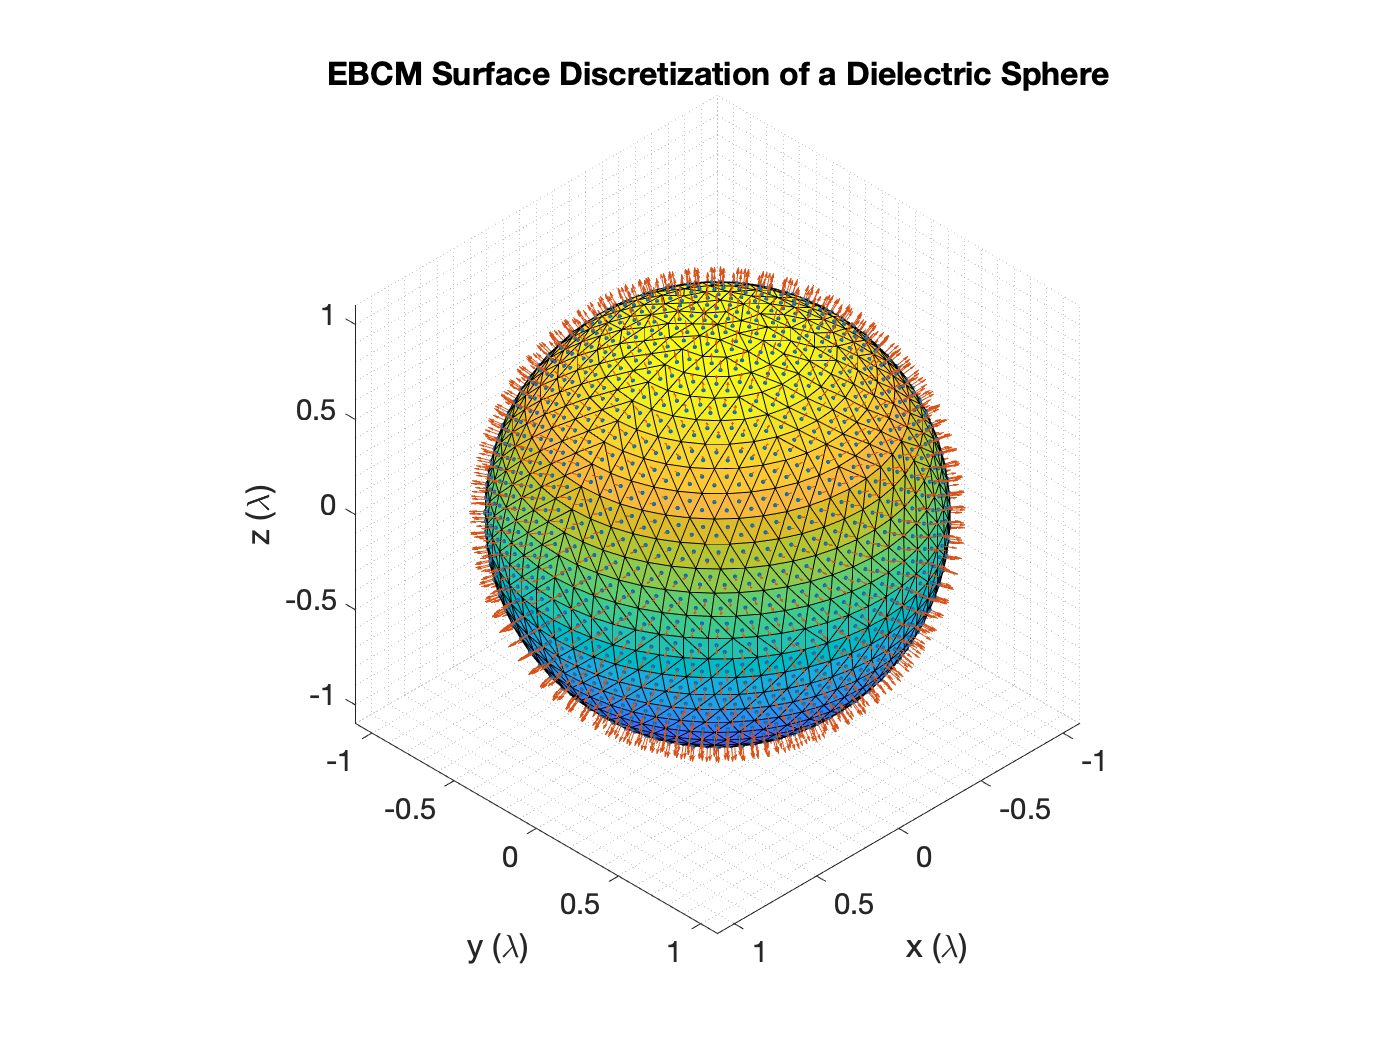
\includegraphics[width=5in]{Tmatrix/Figures/ebcmsphere}} \\
   \subfigure{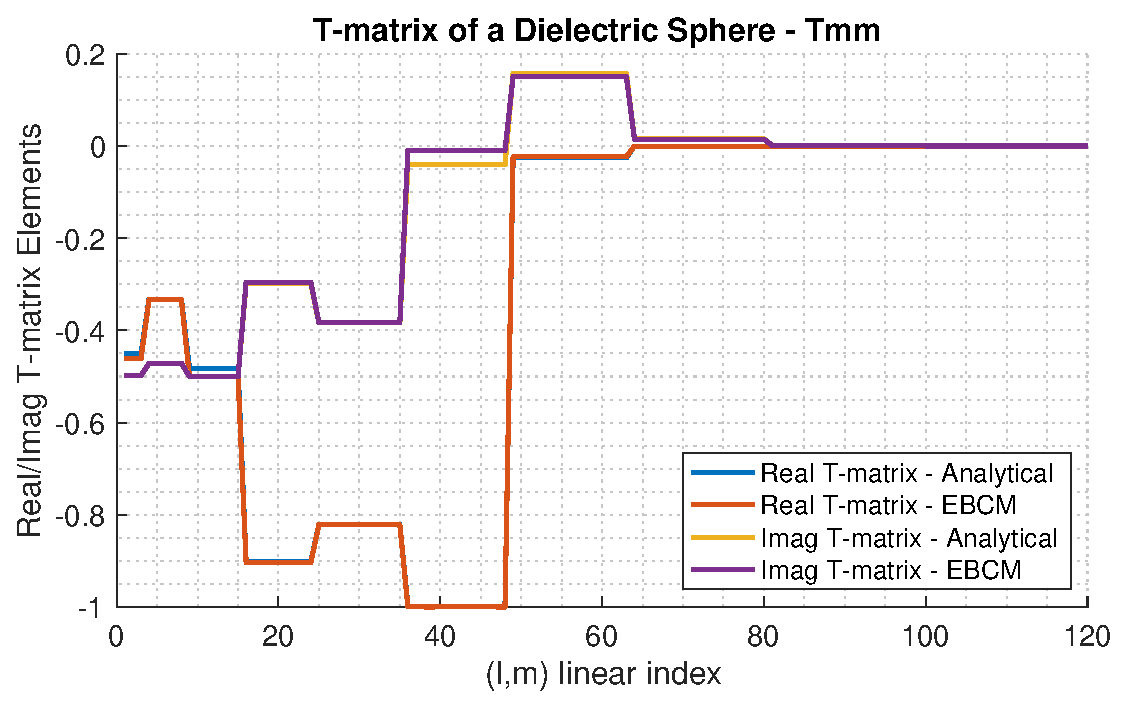
\includegraphics[width=2.9in]{Tmatrix/Figures/ebcmTmm}}
   \subfigure{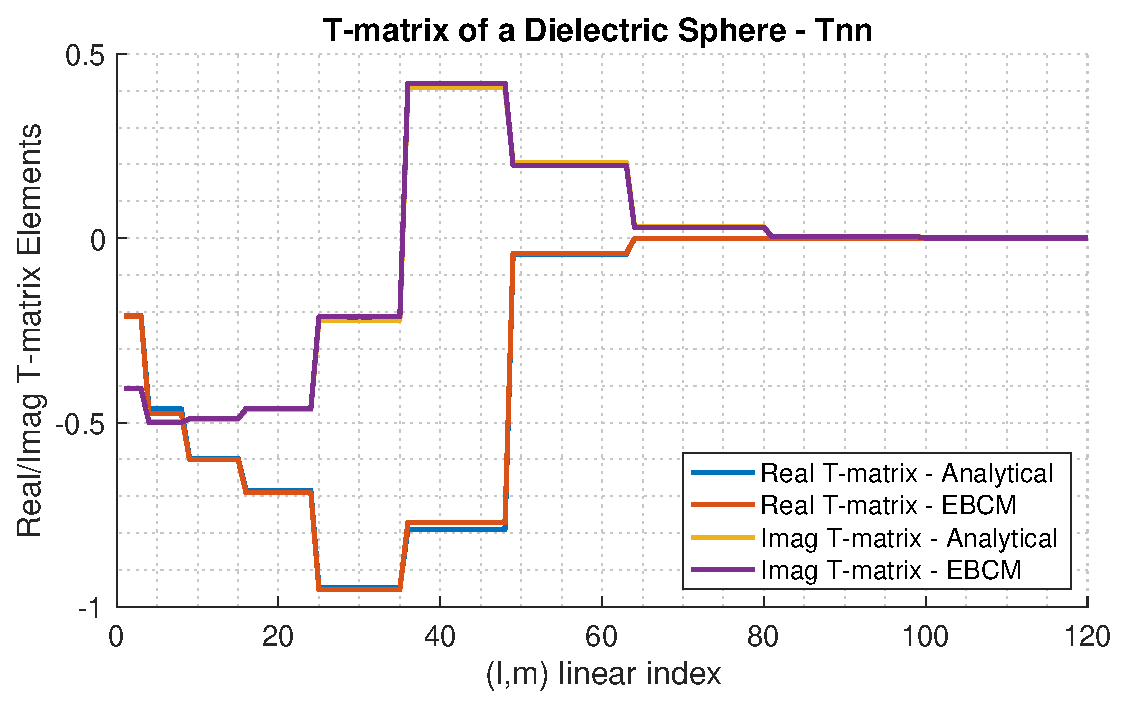
\includegraphics[width=2.9in]{Tmatrix/Figures/ebcmTnn}}
   \caption{Top: Surface discretization of a dielectric sphere for the EBCM. Sphere has a radius of 1$\lambda$ and a relative permittivity of 2 in a background of free-space. The facet vertices are distributed in a disco ball arraignment. A total of 2192 surface facets are determined from the convex hull of a 3D Delaunay triangularization. Surface normal vectors are shown at the centroid of each facet. The facet centroids are the integration points, $\br'$. Facet area is determined from the cross product of two triangle edge vectors. Bottom: Real and imaginary parts of the diagonal $T^{MM}$ and $T^{NN}$ T-matrices computed with \texttt{ebcm} and compared to the T-matrices computed analytically with \texttt{tmatrixDielectricSphere}. Small differences are apparent. The EBCM result improves with finer surface discretization. }
   \label{ebcmcompare}
\end{figure}


\clearpage
\paragraph{Routine}

The routine \texttt{ebcm} returns the four block T-matrices computed using the EBCM, \eqref{tmatrixqq}. The T-matrices are square and have harmonics up to maximum degree $L$ all $\pm m$ linearly indexed. The routine takes as input the wavenumbers, $k_1$ and $k_2$, in the outer and inner regions, respectively, the maximum degree harmonic, $L$, and user-provided surface discretization. The surface discretization needs the Cartesian coordinates of surface points, $\br'$, the differential area at each point, $dS'$, and the Cartesian components of the outward surface unit normal vector, $\hat{n}'$, at each point. The arrays describing the surface can be any size, but must be the same size. The permeabilities, $\mu_1$ and $\mu_2$, are optional, and default to 1, and when needed, they can be relative or absolute, but must also be included in $k_1$ and $k_2$. The matrices $\textit{Rg}\overline{\bb{Q}}$ and $\overline{\bb{Q}}$ are computed as running sums over surface points in order to limit the total size of temporary arrays. The matrix inverse, $\overline{\bb{Q}}^{-1}$, is computed with Matlab's right matrix divide, \texttt{'/'}.  Two helper functions, \texttt{ebcmbessel} and \texttt{ebcmprod}, are used to organize the code and compute combinations of spherical Bessel and angular functions. The results match the analytic expressions derived for the T-matrix of a dielectric sphere, shown in Figure \ref{ebcmcompare}. 


{\footnotesize
\VerbatimInput{\code/Tmatrix/ebcm.m}
}


%\ea{\bb{E}_{inc}(\br) &=& \sum_{l=1}^{\infty}\sum_{m=-l}^l a_{lm} \textit{Rg}\M{k_1,\br}  + b_{lm}\textit{Rg}\N{k_1,\br} \nonumber \\
%\ & =& -\int_S dS'\left( i \omega \mu_1 \left(ik_1\sum_{l=1}^{\infty}\sum_{m=-l}^l \textit{Rg}\M{k_1,\br}\Mhat{k_1,\br'} + \textit{Rg}\N{k_1,\br}\Nhat{k_1,\br'}\right) \cdot \hat{n}' \times \bb{H}_1(\br') -\right. \nonumber \\
%\ &=& \left. \left[\nabla'\times \left(ik_1\sum_{l=1}^{\infty}\sum_{m=-l}^l \textit{Rg}\M{k_1,\br}\Mhat{k_1,\br'} + \textit{Rg}\N{k_1,\br}\Nhat{k_1,\br'}\right)  \right] \cdot \hat{n}' \times \bb{E}_1(\br') \right) }
%
%\ea{a_{lm} &=& -ik_1 \int_S dS'\left( i \omega \mu_1 \left(\sum_{l=1}^{\infty}\sum_{m=-l}^l \textit{Rg}\M{k_1,\br}\Mhat{k_1,\br'} + \textit{Rg}\N{k_1,\br}\Nhat{k_1,\br'}\right) \cdot \hat{n}' \times \bb{H}_1(\br') -\right. \nonumber \\
%\ & & \left. \left[\nabla'\times \left(\sum_{l=1}^{\infty}\sum_{m=-l}^l \textit{Rg}\M{k_1,\br}\Mhat{k_1,\br'} + \textit{Rg}\N{k_1,\br}\Nhat{k_1,\br'}\right)  \right] \cdot \hat{n}' \times \bb{E}_1(\br') \right) }
%
%
%\ea{b_{lm} &=& -ik_1\int_S dS'\left( i \omega \mu_1 \left(\sum_{l=1}^{\infty}\sum_{m=-l}^l \textit{Rg}\M{k_1,\br}\Mhat{k_1,\br'} + \textit{Rg}\N{k_1,\br}\Nhat{k_1,\br'}\right) \cdot \hat{n}' \times \bb{H}_1(\br') -\right. \nonumber \\
%\ & & \left. \left[\nabla'\times \left( \sum_{l=1}^{\infty}\sum_{m=-l}^l \textit{Rg}\M{k_1,\br}\Mhat{k_1,\br'} + \textit{Rg}\N{k_1,\br}\Nhat{k_1,\br'}\right)  \right] \cdot \hat{n}' \times \bb{E}_1(\br') \right) }
%
%
%\ea{a_{lm} &=& -ik_1 \int_S dS'\left( i \omega \mu_1 \left(  \Mhat{k_1,\br'}  \right) \cdot \hat{n}' \times \bb{H}_1(\br') -  \left[\nabla'\times \left( \Mhat{k_1,\br'}  \right)  \right] \cdot \hat{n}' \times \bb{E}_1(\br') \right) }
%
%\ea{b_{lm} &=& -ik_1\int_S dS'\left( i \omega \mu_1 \left(   \Nhat{k_1,\br'}\right) \cdot \hat{n}' \times \bb{H}_1(\br') - \left[\nabla'\times \left( \Nhat{k_1,\br'}\right)  \right] \cdot \hat{n}' \times \bb{E}_1(\br') \right) }

\clearpage
\newpage

\section{T-matrix to S-matrix Transformation}
\label{secTtoS}

Here we derive the relationship between the T-matrix and S-matrix. Start with the expression for the scattered field, \eqref{tmatrixesca}, then write out the sums and expand the vector wave functions in their far-field approximations, \eqref{farfieldM} and \eqref{farfieldN}, 
\eq{\lim_{kr \rightarrow \infty} \bb{E}_s(\hat{k}_s) = \dfrac{e^{ikr}}{kr}  \sum_{l=1}^{\infty}\sum_{m=-l}^l i^{-l-1} c_{lm} \bb{C}_{lm}(\theta_s,\phi_s) +  i^{-l}   d_{lm}  \bb{B}_{lm}(\theta_s,\phi_s) }

Substituting the definition of the T-matrix
\ea{ \bb{E}_s(\hat{k}_s) &=& \dfrac{e^{ikr}}{kr}  \sum_{lm}\sum_{l'm'} i^{-l-1} \bb{C}_{lm}(\theta_s,\phi_s)\left(T^{MM}_{lm,l'm'} a_{l'm'} + T^{MN}_{lm,l'm'} b_{l'm'}  \right)   \nonumber \\
\ & \ & + i^{-l}   \bb{B}_{lm}(\theta_s,\phi_s)\left(T^{NM}_{lm,l'm'} a_{l'm'} + T^{NN}_{lm,l'm'} b_{l'm'}  \right)  }

The coefficients $a_{lm}$ and $b_{lm}$ are chosen as the expansion coefficients for the vector plane waves, \eqref{almplaneE} and \eqref{blmplaneE}, giving 
\ea{\bb{E}_s(\hat{k}_s) &=& 4\pi\dfrac{e^{ikr}}{kr}  \sum_{lm}\sum_{l'm'} i^{-l-1} \bb{C}_{lm}(\theta_s,\phi_s)\left(T^{MM}_{lm,l'm'} i^{l'}  \bb{C}^*_{l'm'}(\theta_i,\phi_i)  + T^{MN}_{lm,l'm'} i^{l'+1}  \bb{B}^*_{l'm'}(\theta_i,\phi_i)  \right)\cdot  \bb{E}_i   \nonumber \\
\ & \ &  + i^{-l}   \bb{B}_{lm}(\theta_s,\phi_s)\left(T^{NM}_{lm,l'm'} i^{l'}  \bb{C}^*_{l'm'}(\theta_i,\phi_i)  + T^{NN}_{lm,l'm'} i^{l'+1}  \bb{B}^*_{l'm'}(\theta_i,\phi_i)  \right)\cdot  \bb{E}_i  \label{scattmatrix1}  }

\noindent where $(\theta_i,\phi_i)$ are the spherical angles of the incident field direction, and $\bb{E}_i$ is the polarized incident electric field.  At this point, the sum can be computed directly and dotted with the polarization unit vectors as needed.  This is written more clearly in matrix notation over the $\theta$, $\phi$ components of the fields as
\ea{\twobyone{E_{s,\theta}(\hat{k}_s)}{E_{s,\phi}(\hat{k}_s)} &=& 4\pi\dfrac{e^{ikr}}{kr} \twobytwo{\bb{C}_{\theta}^t(\theta_s,\phi_s)}{\bb{B}_{\theta}^t(\theta_s,\phi_s)}{\bb{C}_{\phi}^t(\theta_s,\phi_s)}{\bb{B}_{\phi}^t(\theta_s,\phi_s)}
\twobytwo{\overline{\bb{L}}_1}{0}{0}{\overline{\bb{L}}_2} 
\tbt{\overline{\bb{T}}^{MM}}{\overline{\bb{T}}^{MN} }{\overline{\bb{T}}^{NM}}{\overline{\bb{T}}^{NN}}  \nonumber \\
\ & \ & \twobytwo{\overline{\bb{L}}_2^{-1}}{0}{0}{\overline{\bb{L}}_1^{-1}} \twobytwo{\bb{C}_{\theta}^*(\theta_i,\phi_i) }{\bb{C}_{\phi}^*(\theta_i,\phi_i) }{\bb{B}_{\theta}^*(\theta_i,\phi_i) } {\bb{B}_{\phi}^*(\theta_i,\phi_i) } \twobyone{E_{i,\theta}(\hat{k}_i)}{E_{i,\phi}(\hat{k}_i)} \label{scattmatrix} }

The vector spherical harmonics are column vectors over harmonics $(l,m)$ (where $^t$ is transpose and $^*$ is simple conjugate). The coefficient matrices $\bb{L}$ are diagonal with elements
\ea{\left[ \overline{\bb{L}}_1\right]_{ll} &=& i^{-l-1}  \\
\left[ \overline{\bb{L}}_2\right]_{ll} &=& i^{-l} }


%4\pi i^l  \bb{C}^*_{lm}(\theta_k,\phi_k)  \cdot  \bb{E} 
%-4\pi i^{l+1}  \bb{B}^*_{lm}(\theta_k,\phi_k) \cdot  \bb{E} 

Choosing the orthonormal basis formed by the spherical unit vectors $\hat{k} = \hat{r}$, $\hat{\theta}$, and $\hat{\phi}$, the scattered field can be written 
\eq{\bb{E}_s = \left( \hat{\theta}_s E_{\theta,s} + \hat{\phi}_s E_{\phi,s} \right) \dfrac{e^{ikr}}{r}}
From which we have the S-matrix 

\begin{equation}
\twobyone{E_{s,\theta}(\hat{k}_s)}{E_{s,\phi}(\hat{k}_s)} = 
\twobytwo
{S_{\theta\theta}(\hat{k}_s,\hat{k}_i) }
{S_{\theta\phi}(\hat{k}_s,\hat{k}_i) }
{S_{\phi\theta}(\hat{k}_s,\hat{k}_i) }
{S_{\phi\phi}(\hat{k}_s,\hat{k}_i) }   
\twobyone{E_{i,\theta}(\hat{k}_i)}{E_{i,\phi}(\hat{k}_i)} 
\end{equation}


%Here, $\hat{\theta}$, and $\hat{\phi}$ are the same as the $\hat{h}$ and $\hat{v}$ polarizations in the 'wave-oriented' or 'forward scattering alignment' (FSA) polarization convention \cite{ulaby2014microwave}, relative to the z-axis. 

%We essentially derived the relation between the T-matrix and the S-matrix in \eqref{scattmatrix} by writing the scattered field using the far-field vector wave functions and coefficients for the vector incident plane waves. 

Further vectorizing \eqref{scattmatrix} over incident and scattered directions, the T-matrix to S-matrix transformation can be written in block matrices, where the block vector spherical harmonics have harmonic indices along rows and wave vector directions along columns. The component S-matrix blocks are
\eq{\twobytwo
{\overline{\bb{S}}_{\theta\theta} }
{\overline{\bb{S}}_{\theta\phi}}
{\overline{\bb{S}}_{\phi\theta} }
{\overline{\bb{S}}_{\phi\phi} }   
=
\dfrac{4\pi}{k} \twobytwo{\overline{\bb{C}}_{\theta}}{\overline{\bb{B}}_{\theta}}{\overline{\bb{C}}_{\phi}}{\overline{\bb{B}}_{\phi}}\twobytwo{\overline{\bb{L}}_1}{0}{0}{\overline{\bb{L}}_2} \tbt{\overline{\bb{T}}^{MM}}{\overline{\bb{T}}^{MN} }{\overline{\bb{T}}^{NM}}{\overline{\bb{T}}^{NN}}  \twobytwo{\overline{\bb{L}}_2^{-1}}{0}{0}{\overline{\bb{L}}_1^{-1}} \twobytwo{\overline{\bb{C}}_{\theta}^*}{\overline{\bb{C}}_{\phi}^*}{\overline{\bb{B}}_{\theta}^* } {\overline{\bb{B}}_{\phi}^*} \label{TtoSBC}} 

\noindent where here $^*$ is conjugate transpose. The S-matrix block matrices have scattered field directions along rows, and incident field directions along columns. Recall that the left vector spherical harmonics are evaluated at scattered directions, and the right ones are evaluated at incident directions. This can be used to compute the S-matrix at arbitrary combinations of incident and scattered directions. Also the vector spherical harmonics are fully normalized.  See Section \ref{fastTtoS} for an exact computation of this using spherical harmonic transforms when the S-matrix can be sampled on the nodes of Gaussian quadrature. 

The routine \texttt{compute\char`_S\char`_from\char`_T}, computes the four spherical vector components of the S-matrix given the four components of the T-matrix. The block T-matrices are $N \times N$ with harmonics up to degree $L$ all $m$ linearly indexed. The routine takes the incident and scattered directions, which can be different sizes between them. The size of the output S-matrix block matrices is size of an array that is the concatenation of the scattered and incident direction array in that order. The fully normalized vector spherical harmonics are used. The matrix multiplication is fast, but the routine can run out of memory quickly for large $L$ and large number of wave directions. The routine gives identical results to the ones in Section \ref{fastTtoS} based on Gaussian quadrature.

{\footnotesize
\VerbatimInput{\code/Tmatrix/compute_S_from_T.m}
}


\section{S-matrix to T-matrix Transformation}
\label{secStoT}

The S-matrix to T-matrix transformation requires integrating the S-matrix components and vector spherical harmonics over the unit spheres of incident and scattered directions. Let the diagonal matrix $\overline{\bb{W}}$ hold the weights of the discretized surface integral over the sphere, where the integral is applied over the sphere of wave vector directions. From orthogonality of the fully normalized vector spherical harmonics, we have the identity
\eq{ \twobytwo{\overline{\bb{C}}_{\theta}^*}{\overline{\bb{C}}_{\phi}^*}{\overline{\bb{B}}_{\theta}^* } {\overline{\bb{B}}_{\phi}^*} 
\twobytwo{\overline{\bb{W}}}{0}{0}{\overline{\bb{W}}} 
\twobytwo{\overline{\bb{C}}_{\theta}}{\overline{\bb{B}}_{\theta}}{\overline{\bb{C}}_{\phi}}{\overline{\bb{B}}_{\phi}} 
= \twobytwo{\overline{\bb{I}}}{0}{0}{\overline{\bb{I}}} } 

This identity assumes that the weights are chosen so that the integral is computed exactly. Using this, \eqref{TtoSBC} can be manipulated to give

\eq{\tbt{\overline{\bb{T}}^{MM}}{\overline{\bb{T}}^{MN} }{\overline{\bb{T}}^{NM}}{\overline{\bb{T}}^{NN}}  
=
\dfrac{k}{4\pi} 
\twobytwo{\overline{\bb{L}}_1^{-1}}{0}{0}{\overline{\bb{L}}_2^{-1}} 
\twobytwo{\overline{\bb{C}}_{\theta}^*}{\overline{\bb{C}}_{\phi}^*}{\overline{\bb{B}}_{\theta}^* } {\overline{\bb{B}}_{\phi}^*} 
\twobytwo{\overline{\bb{W}}}{0}{0}{\overline{\bb{W}}} 
\twobytwo
{\overline{\bb{S}}_{\theta\theta} }
{\overline{\bb{S}}_{\theta\phi}}
{\overline{\bb{S}}_{\phi\theta} }
{\overline{\bb{S}}_{\phi\phi} }   
\twobytwo{\overline{\bb{W}}}{0}{0}{\overline{\bb{W}}} 
\twobytwo{\overline{\bb{C}}_{\theta}}{\overline{\bb{B}}_{\theta}}{\overline{\bb{C}}_{\phi}}{\overline{\bb{B}}_{\phi}} 
\twobytwo{\overline{\bb{L}}_2}{0}{0}{\overline{\bb{L}}_1} \label{StoTBC}}

This expression transforms the S-matrix to the T-matrix under the condition that the S-matrix is fully sampled and can be accurately integrated with $\overline{\bb{W}}$. See Section \ref{fastStoT} for a fast routine that computes this integral exactly when the S-matrix is sampled at the nodes of Gaussian quadrature. 

\section{Far-field T-matrix}

In \eqref{TtoSBC} the inner three matrices of the T-matrix to S-matrix transformation convert between vector spherical harmonic expansions on either side of the T-matrix. From this, it is possible to define a far-field T-matrix that transforms between incoming and outgoing far-field plane-wave patterns that are expressed in vector spherical harmonics.

Let an incoming far-field pattern of a field and its vector spherical harmonic expansion be defined
\begin{eqnarray}
\bb{F}(\theta,\phi) &=& F_{\theta}(\theta,\phi) \hat\theta + F_{\phi}(\theta,\phi) \hat\phi \\
\ & = & \sum_{l=1}^{L} \sum_{m = -l}^{l} b_{lm} \bb{B}_{lm}(\theta,\phi) + c_{lm} \bb{C}_{lm}(\theta,\phi)
\end{eqnarray}

\noindent and let an outgoing far-field pattern due to a scatterer and its vector spherical harmonic expansion be
\begin{eqnarray}
\bb{F}'(\theta,\phi) &=& F_{\theta}'(\theta,\phi) \hat\theta + F_{\phi}'(\theta,\phi) \hat\phi \\
\ & = & \sum_{l=1}^{L} \sum_{m = -l}^{l} b_{lm}' \bb{B}_{lm}(\theta,\phi) + c_{lm}' \bb{C}_{lm}(\theta,\phi)
\end{eqnarray}

Both field expansions are band limited with the same number of harmonics. Define the far-field T-matrix to transform the vector spherical harmonic coefficients of the incoming field to those of the outgoing field:
\begin{equation}
\twobyone{\bb{b}'}{\bb{c}'} = \twobytwo{\overline{\bb{T}}^{BB}}{\overline{\bb{T}}^{BC}}{\overline{\bb{T}}^{CB}}{\overline{\bb{T}}^{CC}}\twobyone{\bb{b}}{\bb{c}} \label{TBC}
\end{equation}

Using \eqref{TtoSBC}, this is related to the full T-matrix as
\eq{
\twobytwo{\overline{\bb{T}}^{BB}}{\overline{\bb{T}}^{BC}}{\overline{\bb{T}}^{CB}}{\overline{\bb{T}}^{CC}}= \dfrac{4\pi}{k} \twobytwo{\overline{\bb{L}}_2}{0}{0}{\overline{\bb{L}}_1} \tbt{\overline{\bb{T}}^{NN}}{\overline{\bb{T}}^{NM}}  {\overline{\bb{T}}^{MN} }{\overline{\bb{T}}^{MM}}\twobytwo{\overline{\bb{L}}_1^{-1}}{0}{0} {\overline{\bb{L}}_2^{-1}}\label{ffTmatrix}} 

The reverse is accomplished by simple inversion.

The routines  \texttt{convert\char`_T\char`_to\char`_Tfar} and  \texttt{convert\char`_Tfar\char`_to\char`_T} will transform T-matrix to a far-field T-matrix and visa versa. They take as input the four $N \times N$ block matrices, where $N = L^2 + 2L$ and maximum harmonic degree $L$ all $m$ linearly indexed.   


{\footnotesize
\VerbatimInput{\code/Tmatrix/convert_T_to_Tfar.m}
}

{\footnotesize
\VerbatimInput{\code/Tmatrix/convert_Tfar_to_T.m}
}



\section{Radar Cross Section from T-matrix}

The bistatic radar cross section is defined 
\eq{\sigma_{pq}(\hat{k}_s,\hat{k}_i) = \lim_{r \rightarrow \infty} 4\pi r^2 \dfrac{\left\vert \hat{p} \cdot \bb{E}_s \right\vert^2}{\left\vert \hat{q} \cdot \bb{E}_i \right\vert^2} \label{rcs1} }

This is used with \eqref{scattmatrix1} to compute the radar cross section given an object T-matrix. In short, the process removes the scale factors $E_o e^{ikr}/r$ from \eqref{scattmatrix1} and can then be evaluated given incident/scattered directions and polarizations.  Because $\sigma_{pq} = 4\pi \vert S_{pq}\vert^2$, \eqref{rcsfromSpq}, the routine \texttt{compute\char`_S\char`_from\char`_T}, Section \ref{secTtoS}, can be used to compute the S-matrix for $\hat{p} = \hat{\theta}$ and $\hat{q} = \hat{\phi}$. This can then be converted to any radar cross section polarization combination using \eqref{projectedsmatrix}. 



\subsection{Backscatter Radar Cross Section of a Sphere}

%\noindent where $\bb{E}_s$ is the far-field scattered field, $\bb{E}_i $ are plane waves incident on the target, and $\hat{p}$ and $\hat{q}$ are polarization unit vectors. 

For a sphere, the radar backscatter is independent of the incident direction, and \eqref{scattmatrix1} can be simplified analytically.  Let the incident direction be in the $+\hat{z}$ direction, $(\theta_i,\phi_i) = (0,0)$, and the scattered direction be $-\hat{z}$ with $(\theta_i,\phi_i) = (\pi,0)$.  Let the incident and scattered electric field have both $\hat{x}$ and $\hat{y}$ components   
\eq{\bb{E}_i = E_x \hat{x} + E_y \hat{y}}

%\ea{\bb{E}_s(\br) &=& 4\pi\dfrac{e^{ikr}}{kr}  \sum_{lm}\sum_{l'm'} \nonumber \\
%\ & \ & i^{-l-1} \bb{C}_{lm}(\pi,0)\left(T^{MM}_{lm,l'm'} i^{l'}  \bb{C}^*_{l'm'}(0,0)  + T^{MN}_{lm,l'm'} i^{l'+1}  \bb{B}^*_{l'm'}(0,0)  \right)\cdot  \bb{E}_i   + \nonumber \\
%\ & \ &  i^{-l}   \bb{B}_{lm}(\pi,0)\left(T^{NM}_{lm,l'm'} i^{l'}  \bb{C}^*_{l'm'}(0,0)  + T^{NN}_{lm,l'm'} i^{l'+1}  \bb{B}^*_{l'm'}(0,0)  \right)\cdot  \bb{E}_i  \nonumber \\ }


For a PEC or dielectric sphere, the T-matrix is diagonal with zero cross terms so that \eqref{scattmatrix} reduces to one sum as 
\ea{\bb{E}_s(\pi,0) &=& -4\pi i\dfrac{e^{ikr}}{kr}   \sum_{lm}\bb{C}_{lm}(\pi,0)T^{MM}_{lm} \bb{C}^*_{lm}(0,0) \cdot  \bb{E}_i   -  \bb{B}_{lm}(\pi,0)T^{NN}_{lm}  \bb{B}^*_{lm}(0,0) \cdot  \bb{E}_i  }

%\ea{\bb{E}_s(\br) &=& 4\pi\dfrac{e^{ikr}}{kr}  \sum_{lm}\nonumber \\
%\ & \ & i^{-l-1} \bb{C}_{lm}(\pi,0)\left(T^{MM}_{lm} i^{l}  \bb{C}^*_{lm}(0,0) \right)\cdot  \bb{E}_i   + \nonumber \\
%\ & \ &  i^{-l}   \bb{B}_{lm}(\pi,0)\left( T^{NN}_{lm} i^{l+1}  \bb{B}^*_{lm}(0,0)  \right)\cdot  \bb{E}_i  \nonumber \\ }
Using \eqref{clmzplus}, \eqref{blmzplus}, \eqref{clmzminus}, \eqref{blmzminus}, this reduces to
\ea{\bb{E}_s(\pi,0) &=& \dfrac{-i}{2} \dfrac{e^{ikr}}{kr}  \sum_{l} (-1)^l (2l+1) \left[ \hat{x} (T^{MM}_{l} - T^{NN}_{l}) E_x - \hat{y} (T^{MM}_{l} - T^{NN}_{l}) E_y\right]\label{esbacksphere} }

This shows that the scattered field in the backscatter direction of a sphere is polarization independent with no cross-pol. Substituting \eqref{esbacksphere} into \eqref{rcs1} and choosing either polarization, the polarization amplitude will cancel. The backscatter radar cross section of a sphere where only the diagonal elements of the T-matrix are non-zero
\eq{\sigma = \dfrac{\pi}{k^2} \left\vert \sum_{l=1}^{\infty} (-1)^l (2l+1) \left(T^{MM}_{l} - T^{NN}_{l}\right) \right\vert^2 \label{rcssphere}}

\subsection{Backscatter RCS of a PEC Sphere}

Substituting the T-matrix for a PEC sphere into \eqref{rcssphere}, the backscatter RCS of a PEC sphere is
\eq{\sigma_{PEC} = \dfrac{\pi}{k^2} \left\vert \sum_{l=1}^{\infty} (-1)^l (2l+1) \left(\dfrac{j_l(ka)}{h_l^{(1)}(ka)}  - \dfrac{[k a j_l(ka)]'}{[k a h_l^{(1)}(ka)]'}\right) \right\vert^2 \label{sigmapec}}


%
%Using the Wronskian
%\eq{j_l(x) {h'}_l^{(1)}(x) - h_l^{(1)}(x) j_l'(x) = \dfrac{i}{x^2} }
%
%\eq{\sigma_{PEC} = \dfrac{\pi}{k^2} \left\vert \sum_{l=1}^{\infty} \dfrac{(-1)^l (2l+1) }{ ka h_l^{(1)}(ka) [k a h_l^{(1)}(ka)]'} \right\vert^2 }
%
%Next, we write this in terms of logarithmic derivative of the Bessel functions.  Let $\chi$ be the Riccati-Bessel function or Riccati-Hankel function.  The logarithmic derivative is 
%
%\eq{\phi_n(x) = x j_n(x)}
%\eq{\zeta_n(x) = xh_n^{(1)}(x)}
%
%\eq{A_n = \dfrac{1}{x j_n(x)}\dd{x j_n(x)}{x}  }
%\eq{B_n = \dfrac{1}{xh_n^{(1)}(x)}\dd{xh_n^{(1)}(x)}{x}}
%
%\eq{\chi_l(x) = xz_l(x)}
%\eq{C_l = \dfrac{1}{\chi_l}\dd{\chi_l}{x} }
%
%These have the single term recurrence 
%
%\eq{\rho_l = \dfrac{\chi_l}{\chi_{l+1}}}
%\eq{\dfrac{1}{\rho_l} = \dfrac{2l+1}{x} - \rho_{l-1}}
%\eq{C_l = -\dfrac{l}{x} + \dfrac{1}{\dfrac{l}{x} - C_{l-1}}}
%
%Using the fact that
%\ea{j_0(x) &=& \dfrac{\sin x}{x} \\
%j_1(x) &=& -\dfrac{\cos x}{x} + \dfrac{\sin x}{x^2} \\
%h_0^{(1)}(x) &=& \dfrac{e^{i x}}{ix} \\
%h_1^{(1)}(x) &=& -\left(1 + \dfrac{i}{x}\right) \dfrac{e^{i x}}{x} }
%
%\eq{\psi_0 = \dfrac{e^{ix}}{i}}
%\eq{\rho_0 = \dfrac{x}{1 - ix}}
%\eq{C_0 = 1 + i - \dfrac{1}{x}}
%
%
%
%
%\eq{\sigma_{PEC} = \dfrac{\pi}{k^2} \left\vert \sum_{l=1}^{\infty} \dfrac{(-1)^l (2l+1) }{\chi_l^2 C_l  } \right\vert^2 }


%
%
%\eq{z'_l(x) = z_{l-1}(x) - \dfrac{l}{x}z_{l}(x) }
%this becomes
%\eq{\sigma_{PEC} = \dfrac{\pi}{k^2} \left\vert \sum_{l=1}^{\infty} \dfrac{(-1)^l (2l+1) }{ x h_l^{(1)}(x)\left((1-l)h_l^{(1)}(x) + x h_{l-1}^{(1)}(x)\right) } \right\vert^2 }
%
%$x = ka$.  The Hankel function can be computed recursively as 
%\eq{z_l(x) = \dfrac{2(l-1)}{x} z_{l-1}(x) - z_{l-2}(x)}
%
%with initial conditions
%\ea{h_0^{(1)}(x) &=& \dfrac{e^{i x}}{ix} \\
%h_1^{(1)}(x) &=& -\left(1 + \dfrac{i}{x}\right) \dfrac{e^{i x}}{x} }


\begin{figure}[H] 
   \centering
   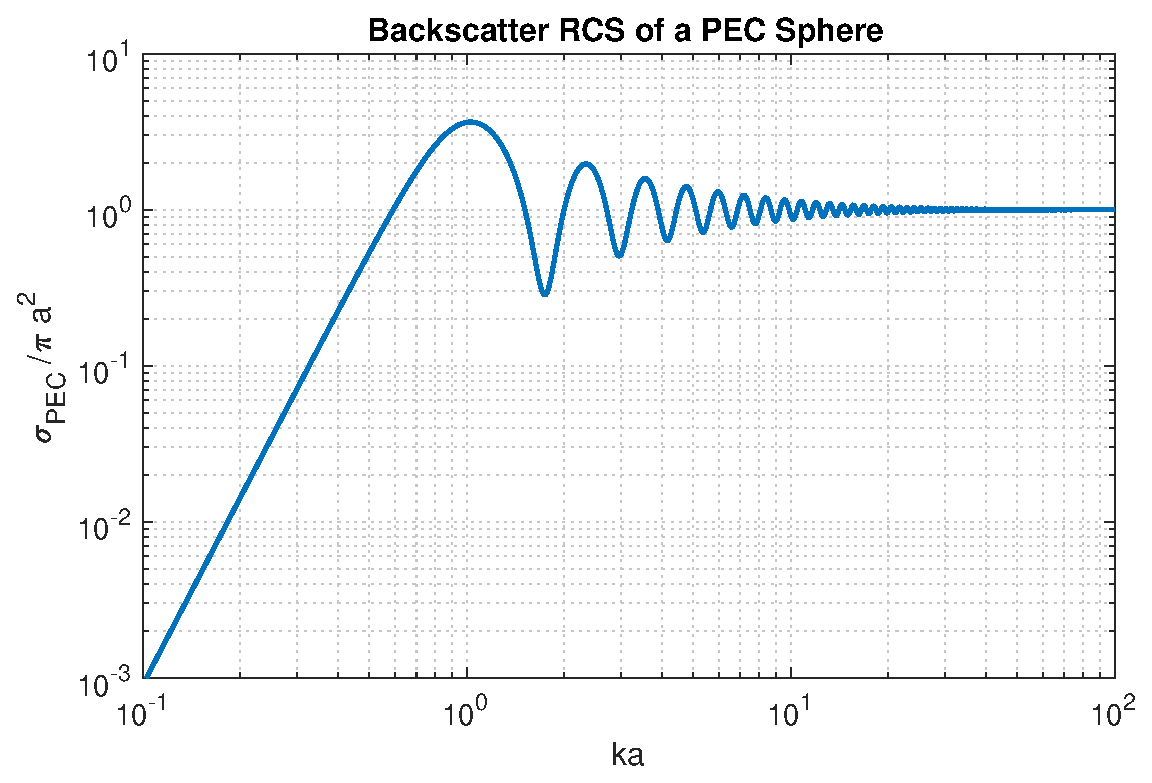
\includegraphics[width=3.5in]{Tmatrix/Figures/brcspecsphere} 
   \caption{RCS of PEC sphere, normalized by cross-section area.  The maximum occurs at $ka \approx 1.03$, with a value of about 3.65 (linear).}
\end{figure}


The routine \texttt{brcs\_pec\_sphere} is a workable routine to compute \eqref{sigmapec}. The sum is truncated when incremental change is less than machine precision. The standard and better way to compute this is to use logarithmic derivatives of the Bessel functions, but that is a separate topic.

{\footnotesize
\VerbatimInput{\code/Tmatrix/brcs_pec_sphere.m}
}

\subsection{Backscatter RCS of a Dielectric Sphere}

Using the T-matirx for the dielectric sphere in \eqref{rcssphere}, the backscatter RCS of a non-magnetic dielectric sphere is 
\eq{\sigma = \dfrac{\pi}{k^2} \left\vert \sum_{l=1}^{\infty} (-1)^l (2l+1) \left(\dfrac{j_2 j_1'  -  j_1j_2'}{ h_1 j_2' -  j_2 h_1'} - \dfrac{ x_2^2 j_2 j_1' -  x_1^2 j_1 j_2' }{ x_1^2 h_1 j_2' - x_2^2  j_2 h_1' } \right) \right\vert^2 \label{sigmaer}}

which uses the shorthand: 
\ea{x_1 &=& k_1 a \\
x_2 &=& k_2 a \\
j_1 &=& j_l(k_1a) \\
j_1' &=& [k_1 a j_l(k_1a)]' \\
j_2 &=& j_l(k_2a) \\
j_2' &=& [k_2 a j_l(k_2a)]' \\
h_1 &=& h_l^{(1)}(k_1a) \\
h_1' &=& [k_1 a h_l^{(1)}(k_1a)]' 
}

\noindent where $k_1$ is the wavenumber outside the sphere, and $k_2$ is wavenumber inside the sphere.  Making use of the Wronskian $j_l(x) {h'}_l^{(1)}(x) - h_l^{(1)}(x) j_l'(x) = i/x^2$, it can be shown that $h_1' j_1 - h_1 j_1'  = i/x_1$.  Then the backscatter can also be written 
\eq{\sigma = \dfrac{\pi}{k^2} \left\vert \sum_{l=1}^{\infty} (-1)^l (2l+1) \left(\dfrac{j_2 j_2' ( x_2^2 - x_1^2) }{x_1 \left(h_1 j_2' - j_2 h_1' \right)\left(x_1^2 h_1 j_2' - x_2^2  j_2 h_1' \right)}\right) \right\vert^2 }


\begin{figure}[h] 
   \centering
   \subfigure{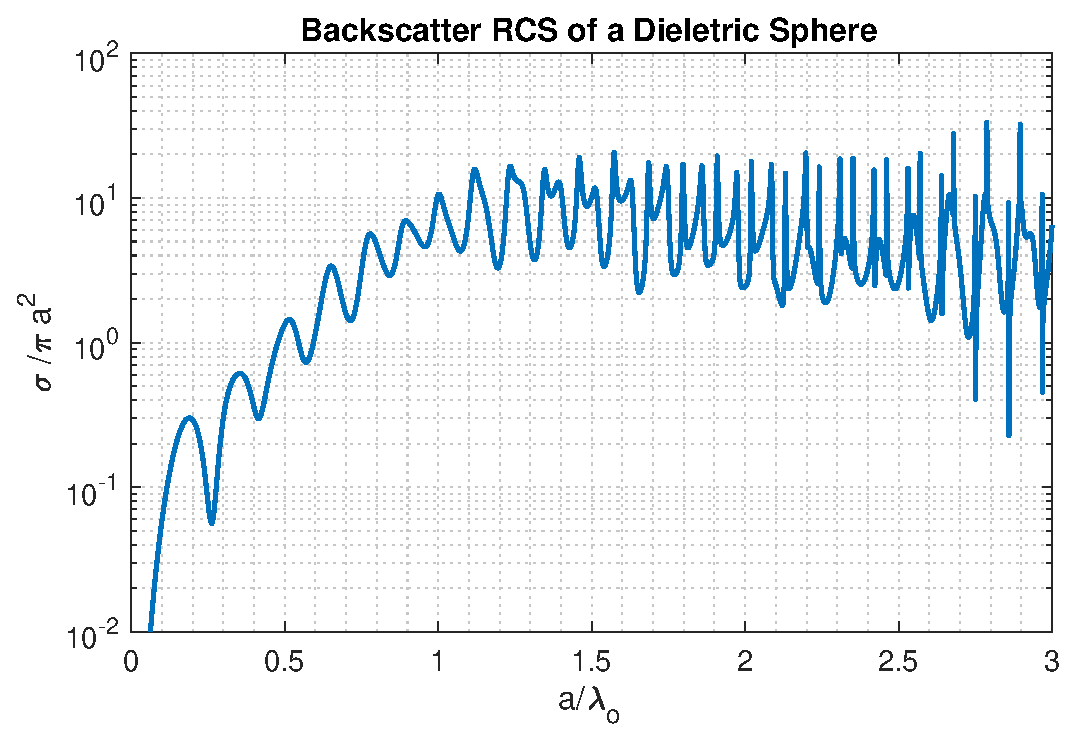
\includegraphics[width=3.2in]{Tmatrix/Figures/brcsdielectricsphere}  \label{brcsdiesph} } 
   \subfigure{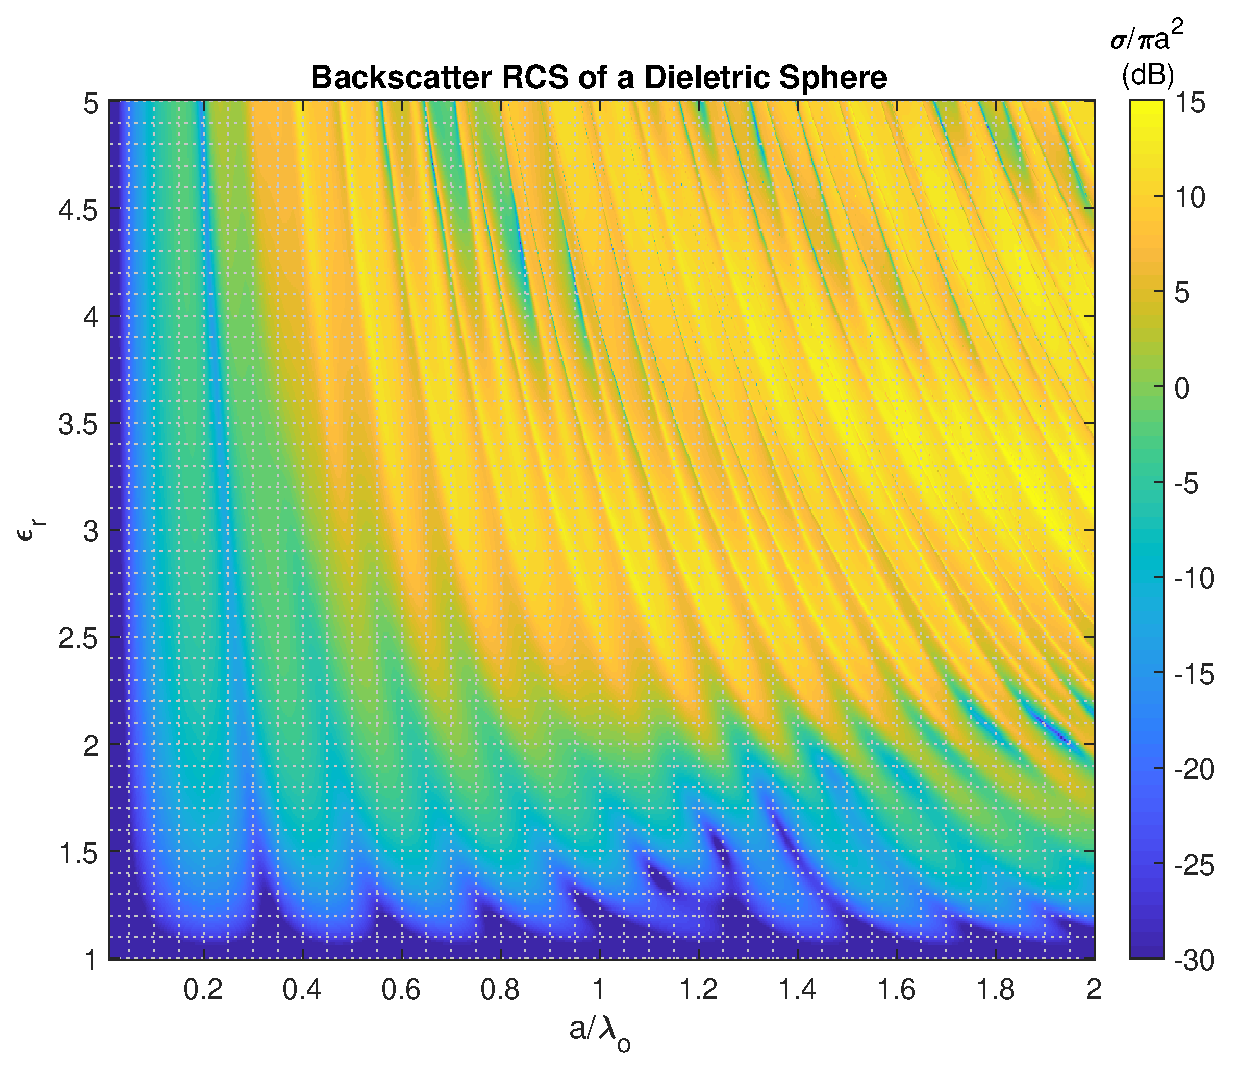
\includegraphics[width=3.1in]{Tmatrix/Figures/brcsdielectricspheregrid}   \label{brcsdiesphall}}
   \caption{Backscatter RCS of dielectric sphere, normalized by cross-section area, in free-space. Left: $\epsilon_r = 2.5$. Right: $\epsilon_r =$1 to 5, and $a/\lambda_o$ = 0 to 2.}
 \end{figure}
%
%
%\begin{figure}[h] 
%   \centering
%   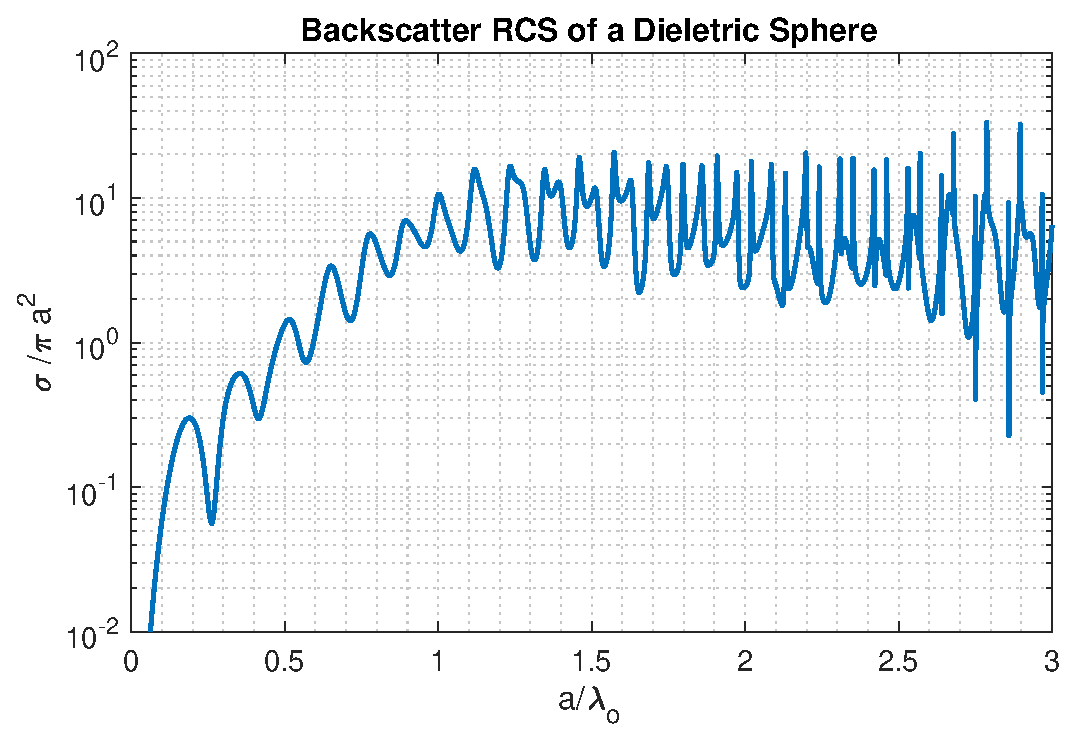
\includegraphics[width=3.5in]{Tmatrix/Figures/brcsdielectricsphere} 
%   \caption{Backscatter RCS of dielectric sphere, normalized by cross-section area, in free-space.  $\epsilon_r = 2.5$.}
%   \label{brcsdiesph}
%\end{figure}
%
%\begin{figure}[h] 
%   \centering
%   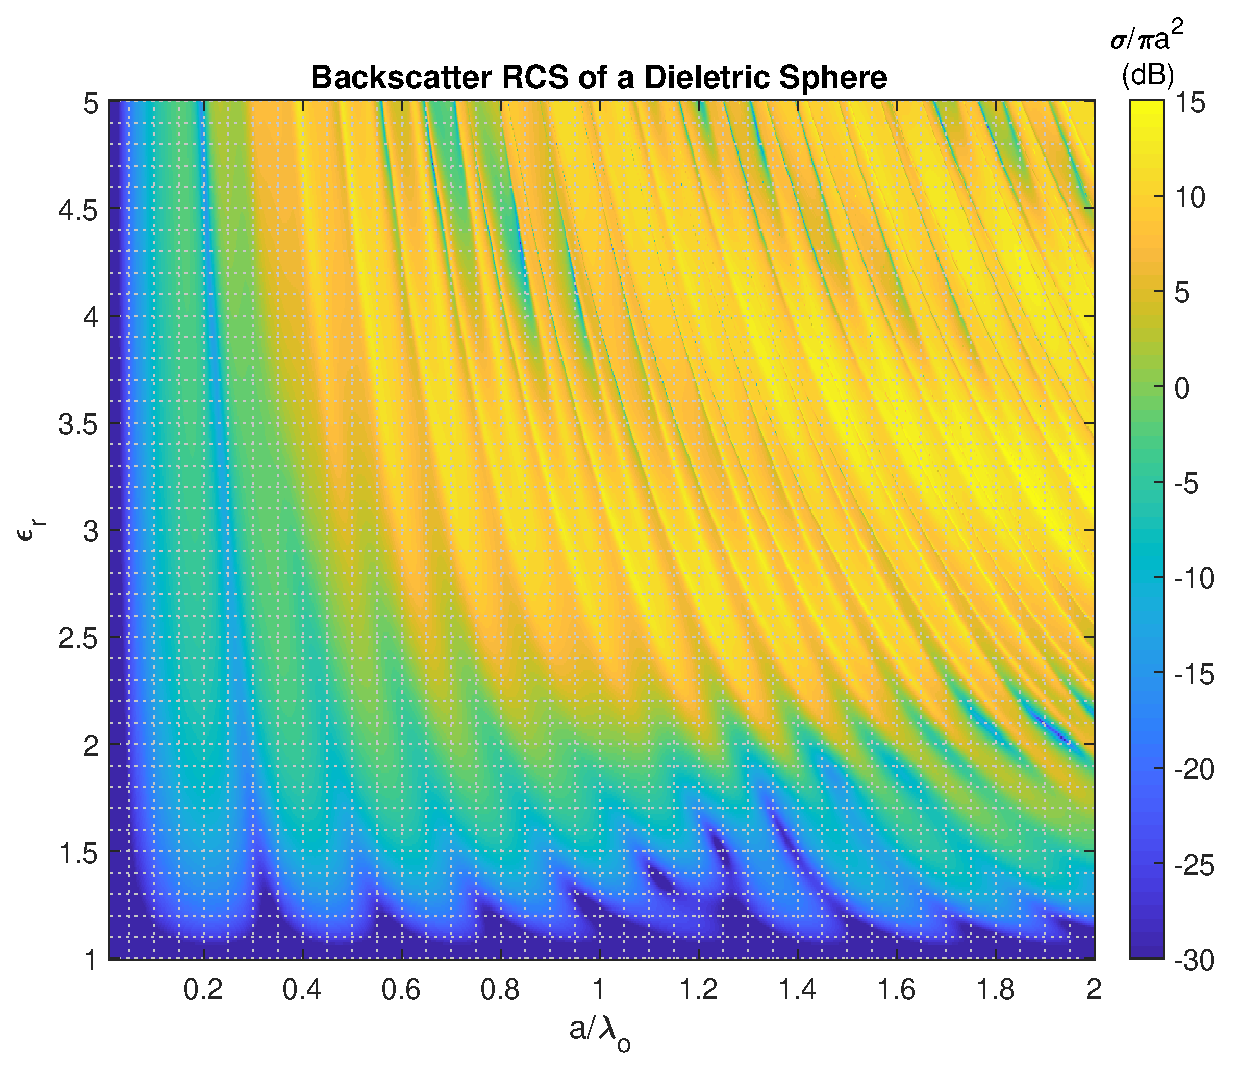
\includegraphics[width=3.5in]{Tmatrix/Figures/brcsdielectricspheregrid} 
%   \caption{Backscatter RCS of lossless dielectric sphere, normalized by cross-section area, in free-space.}
%      \label{brcsdiesphall}
%\end{figure}

The routine \texttt{brcs\_dielectric\_sphere} is a workable routine for the computation of \eqref{sigmaer}.  Assuming a background of vacuum, Figure \ref{brcsdiesph} shows the backscatter RCS for a sphere with $\epsilon_r = 2.5$ as a function of sphere radius. Figure \ref{brcsdiesphall} shows the same as a function of $k_o a$ and $\epsilon_r$. 

\clearpage
{\footnotesize
\VerbatimInput{\code/Tmatrix/brcs_dielectric_sphere.m}
}

\section{Scattering Cross Section from T-matrix}

The scattering cross section is equal to the scattered power integrated over the sphere for a unit amplitude incident electric field and specific incident direction. From \cite{tsang1985theory}, the scattering cross section is written in terms of the S-matrix as 
\eq{\sigma_{s\beta}(\hat{k}_i) = \int_S \left( \vert S_{p \beta}(\hat{k}_s,\hat{k}_i) \vert^2 + \vert S_{q \beta}(\hat{k}_s,\hat{k}_i) \vert^2 \right) d\Omega_s  }

\noindent where $\beta$ is the incident polarization and $p$ and $q$ are any two orthogonal scattered polarizations. Taking the magnitude squared of \eqref{scattmatrix1} without the terms $E_o e^{ikr}/r $, integrating this over the scattered field directions, and applying orthonormality of the vector spherical harmonics, one gets, similar to \cite{tsang1985theory},

\ea{\sigma_{s\beta}(\hat{k}_i) &=& \dfrac{16\pi^2}{k^2} \sum_{lm} \left\{ \left\vert \sum_{l'm'} \left(T^{MM}_{lm,l'm'} i^{l'}  \bb{C}^*_{l'm'}(\theta_i,\phi_i)  + T^{MN}_{lm,l'm'} i^{l'+1}  \bb{B}^*_{l'm'}(\theta_i,\phi_i)  \right)\cdot  \hat{\beta} \right\vert^2 \right. \nonumber \\
\ & \ &  +\left. \left\vert \sum_{l'm'} \left(T^{NM}_{lm,l'm'} i^{l'}  \bb{C}^*_{l'm'}(\theta_i,\phi_i)  + T^{NN}_{lm,l'm'} i^{l'+1}  \bb{B}^*_{l'm'}(\theta_i,\phi_i)  \right)\cdot  \hat{\beta} \right\vert^2 \right\}  \label{tmatrixscatcrosssection} }

The routine \texttt{compute\char`_scs\char`_from\char`_tmatrix} computes the scattering cross section of an object from its T-matrix. It takes as input the four $N \times N$ bock T-matrices where $N = L^2 + 2L$, for harmonics up to maximum degree $L$ all $m$.  The incident angles can be any size. The incident polarization is defined relative to the spherical unit vectors $\hat{\beta} = \cos \beta \hat{\theta} + \sin\beta \hat{\phi}$.  Recall $\hat{v} =\hat{\theta}$ and $\hat{h} =\hat{\phi}$. Values $\beta = [0,\pi/2]$ correspond to $v, h$ respectively. The array of $\beta$ can be any size. The scattering cross section is returned on an array with dimensions that are the concatenation of the sizes of the incident direction array and polarization angle array.  


{\footnotesize
\VerbatimInput{\code/Tmatrix/compute_scs_from_tmatrix.m}
}

% From \cite{tsang2000scattering}, if the scattered electric field is written in terms of the far field pattern as 
%\eq{\bb{E}_s = \left( \hat{v}_s E_{vs
%} + \hat{h}_s E_{hs} \right) \dfrac{e^{ikr}}{r}}
%with 
%\eq{\twobyone{E_{vs}}{E_{hs}} = \twobytwo{S_{vv}}{S_{vh}}{S_{hv}}{S_{hh}} \twobyone{E_{vi}}{E_{hi}}}
%
%then the scattering cross section for polarization $p = v,h$ and fixed incident direction is 
%\eq{\sigma_{sp}(\hat{k}_i) = \int_S \left( \vert S_{vp}(\hat{k}_s,\hat{k}_i) \vert^2 + \vert S_{hp}(\hat{k}_s,\hat{k}_i) \vert^2 \right) d\Omega_s  }

%
%\eq{\bb{E}_s = \hat{e}_s E_o f(\hat{k}_s,\hat{k}_i) \dfrac{e^{ikr}}{r}}
%
%then the scattering cross section is 
%\eq{\sigma_s = \int \left\vert f(\hat{k}_s,\hat{k}_i) \right\vert^2 d\Omega_s} 
%


\subsection{Scattering Cross Section of a Sphere}

For the scattering cross section of a sphere, from symmetry, we only need to consider one incident polarization and an arbitrary incident direction. Assume that the incident plane wave propagates in the $z$ direction:
\eq{\bb{E}_i = E_o \hat{x}  \label{Eincxz}}

The T-matrix of the sphere is diagonal with zero cross terms, which means \eqref{tmatrixscatcrosssection} simplifies to
\ea{\sigma_{s} &=& \dfrac{16\pi^2}{k^2} \sum_{lm} \left\{ \left\vert  T^{MM}_{lmlm}   \bb{C}^*_{lm}(0,0) \cdot  \hat{x} \right\vert^2 + \left\vert T^{NN}_{lmlm}  \bb{B}^*_{lm}(0,0)  \cdot  \hat{x} \right\vert^2 \right\}  }

From \eqref{clmzplus}, \eqref{blmzplus}, and \eqref{Eincxz}, the vector spherical harmonics for $z$ propagation wave have only $m=\pm1$ harmonics and the dot product with $\hat{x}$ is
\eq{\bb{C}^*_{l,\pm 1}(0,0) \cdot  \hat{x}=  \dfrac{i}{2} \sqrt{\dfrac{2l+1}{4\pi}} }
\eq{\bb{B}^*_{l,\pm 1}(0,0) \cdot  \hat{x} = \pm  \dfrac{1}{2} \sqrt{\dfrac{2l+1}{4\pi}} }

Substituting these we get 
%\ea{\sigma_{sx}(\hat{k}_i) &=& \dfrac{16\pi^2}{k^2} \sum_{lm} \left\{ \left\vert  T^{MM}_{lmlm}   \bb{C}^*_{lm}(0,0) \cdot  \hat{x} \right\vert^2 + \left\vert T^{NN}_{lmlm}  \bb{B}^*_{lm}(0,0)  \cdot  \hat{x} \right\vert^2 \right\}  }

% scattered field is 
%\ea{\bb{E}_s(\hat{k}_s) &=& 4\pi\dfrac{e^{ikr}}{kr} i  \sum_{lm}-\bb{C}_{lm}(\theta_s,\phi_s)T^{MM}_{lm} \bb{C}^*_{lm}(0,0) \cdot  \bb{E}_i   +  \bb{B}_{lm}(\theta_s,\phi_s)T^{NN}_{lm}  \bb{B}^*_{lm}(0,0) \cdot  \bb{E}_i  \nonumber \\ }
%
%Using \eqref{clmzplus}, \eqref{blmzplus}, and \eqref{Eincxz}
%
%\eq{\bb{C}^*_{l,\pm 1}(0,0) \cdot  \bb{E}_i = E_o \dfrac{i}{2} \sqrt{\dfrac{2(l+1)}{4\pi}} }
%\eq{\bb{B}^*_{l,\pm 1}(0,0) \cdot  \bb{E}_i = \pm E_o \dfrac{1}{2} \sqrt{\dfrac{2(l+1)}{4\pi}} }
%
%\ea{\bb{E}_s(\hat{k}_s) &=& E_o 4\pi\dfrac{e^{ikr}}{2kr} \sum_{l,m=\pm1} \sqrt{\dfrac{2(l+1)}{4\pi}} \left( \bb{C}_{lm}(\theta_s,\phi_s)T^{MM}_{lm}    \pm i \bb{B}_{lm}(\theta_s,\phi_s)T^{NN}_{lm}  \right) \nonumber \\ }
%%\ea{\bb{E}_s(\br) &=& E_o 4\pi\dfrac{e^{ikr}}{2kr} \sum_{l} \sqrt{\dfrac{2(l+1)}{4\pi}} \left( (\bb{C}_{l,1}(\theta,\phi) + \bb{C}_{l,-1}(\theta,\phi)) T^{MM}_{l}    + i \left( \bb{B}_{l,1}(\theta,\phi) + \bb{B}_{l,-1}(\theta,\phi)\right) T^{NN}_{l}  \right) \nonumber \\ }
%
%Dropping $E_o$ and $e^{ikr}/r$, integrating the magnitude squared of the scattered field over the sphere, 
%
%\ea{\sigma_{sca} &=& \left(\dfrac{4\pi}{2k}\right)^2  \int \left\vert \sum_{l} \sqrt{\dfrac{2(l+1)}{4\pi}} \left( (\bb{C}_{l,1}(\theta_s,\phi_s) + \bb{C}_{l,-1}(\theta_s,\phi_s)) T^{MM}_{l}   \right.\right. \nonumber \\
%\ & \ & \left.\left. + i \left( \bb{B}_{l,1}(\theta_s,\phi_s) + \bb{B}_{l,-1}(\theta_s,\phi_s)\right) T^{NN}_{l}  \right) \right\vert^2 d\Omega_s }
%
%Expanding the magnitude squared as two conjugate independent sums, then after applying orthogonality of the vector spherical harmonics each term becomes independent.  

\eq{\sigma_{s} = \dfrac{2\pi}{k^2}  \sum_{l=1}^{\infty}(2l+1) \left(\left\vert T^{MM}_{l} \right\vert^2 + \left\vert T^{NN}_{l} \right\vert^2  \right) \label{spheresca}  }

A factor of two comes from summing the $m=\pm1$ terms. 

\subsection{Scattering Cross Section of a PEC Sphere}

The scattering cross section of a PEC sphere is given by substituting the T-matrix for a PEC sphere into \eqref{spheresca}
\eq{\sigma_{s,PEC} = \dfrac{2\pi}{k^2}  \sum_{l=1}^{\infty}(2l+1) \left(\left\vert \dfrac{j_l(ka)}{h_l^{(1)}(ka)}  \right\vert^2 + \left\vert \dfrac{[k a j_l(ka)]'}{[k a h_l^{(1)}(ka)]'} \right\vert^2  \right) \label{scspecsphere}}

\noindent where the sphere has radius $a$ in a background with wavenumber $k$.

\begin{figure}[H] 
   \centering
   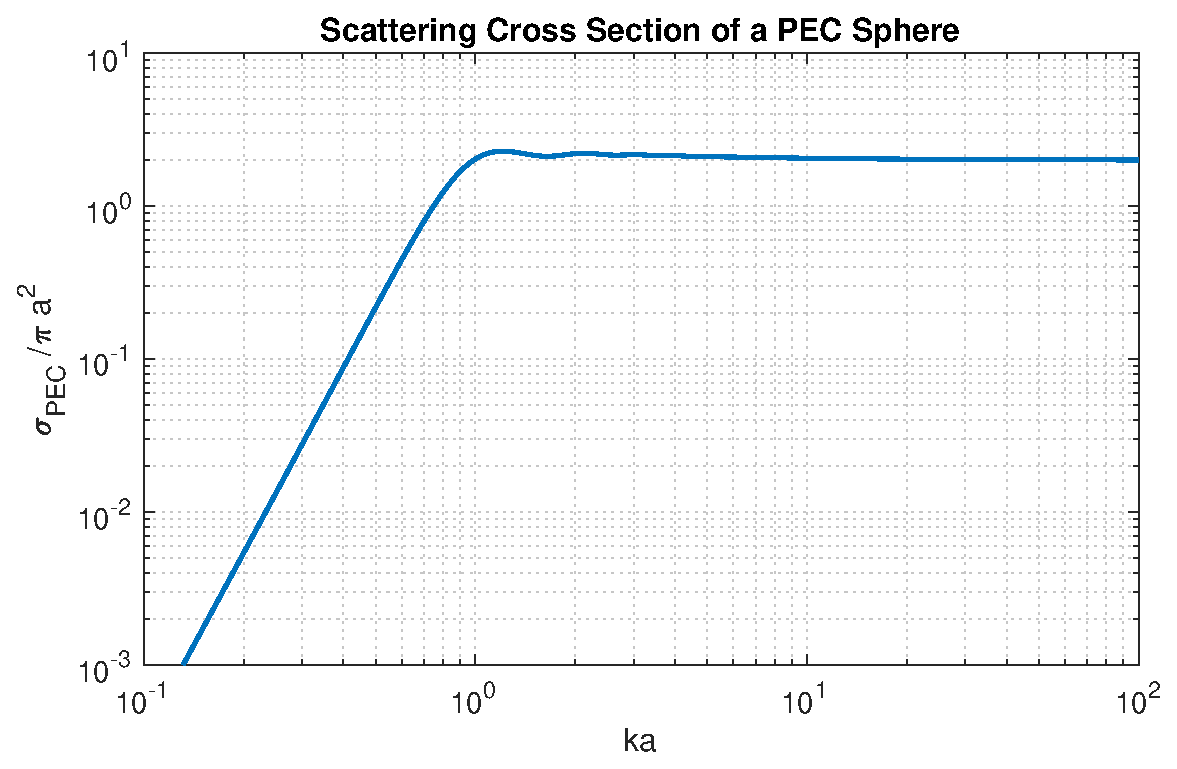
\includegraphics[width=4in]{Tmatrix/Figures/scspecsphere} 
   \caption{Scattering cross section of a PEC sphere, normalized by cross-section area, in free-space.}
   \label{scspecsph}
\end{figure}




The routine \texttt{scs\char`_pec\char`_sphere} is a workable routine to compute \eqref{scspecsphere}. The sum is truncated when incremental change is less than machine precision. 

{\footnotesize
\VerbatimInput{\code/Tmatrix/scs_pec_sphere.m}
}

\subsection{Scattering Cross Section of a Dielectric Sphere}

The scattering cross section of a dielectric sphere is given by substituting the T-matrix for a dielectric sphere into \eqref{spheresca}. This gives identical results to \cite{tsang2000scattering} Figure 1.6.3 and also matches outputs from Ulaby and Long 2014 Code Module 8.12.


\begin{figure}[H] 
   \centering
   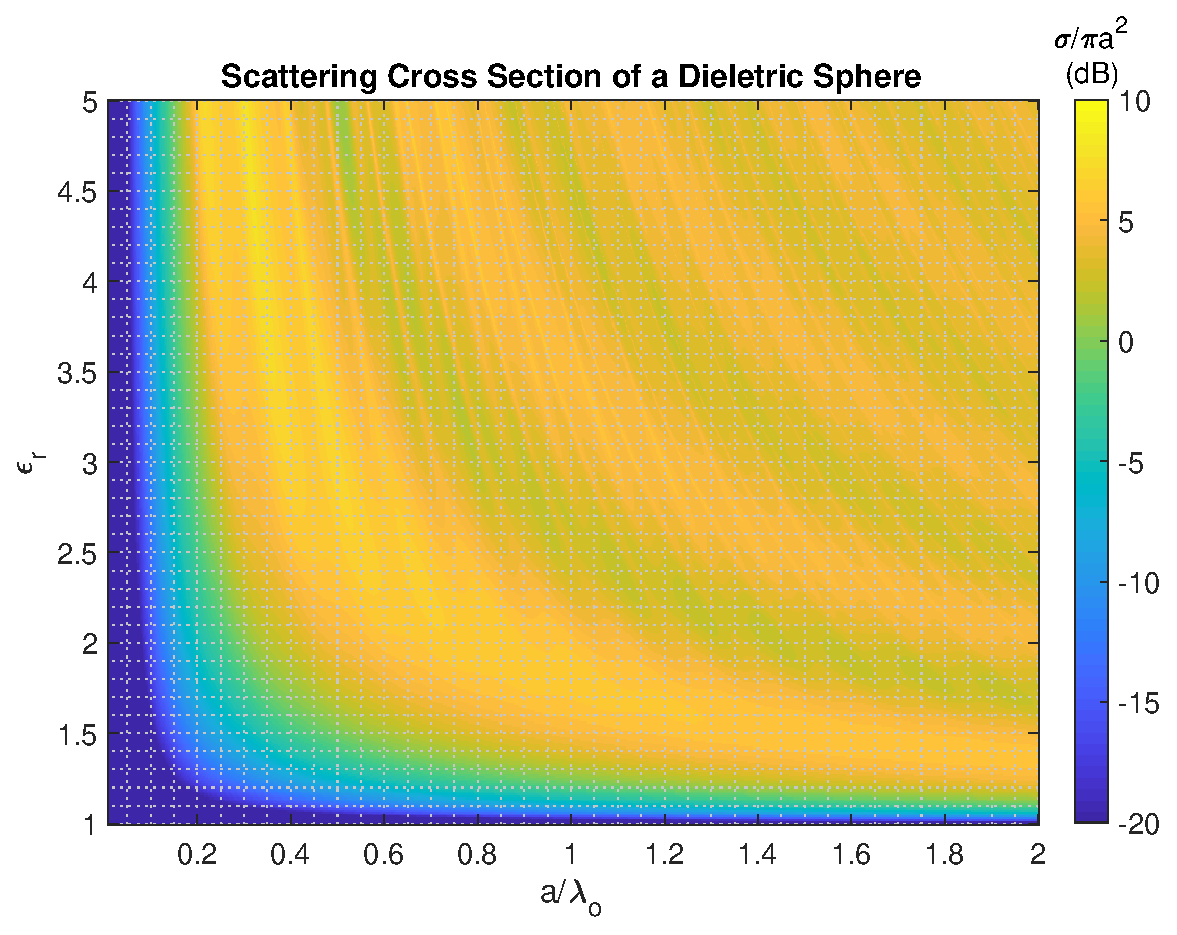
\includegraphics[width=3.5in]{Tmatrix/Figures/scsdielectricspheregrid} 
   \caption{Scattering cross section of lossless dielectric sphere, normalized by cross-section area, in free-space.}
      \label{scsdiesphall}
\end{figure}

\clearpage


The routine \texttt{scs\char`_dielectric\char`_sphere} computes the scattering cross section of a dielectric sphere given the inner and outer wavenumbers $k_1$, $k_2$, and sphere radius $a$.  

{\footnotesize
\VerbatimInput{\code/Tmatrix/scs_dielectric_sphere.m}
}

%
%\subsection{Rayleigh Limit}
%
%Classical Rayleigh scattering comes by taking the small argument limit of \eqref{spheresca}.  Keeping only the $l=1$ term, assuming nonmagnetic.  Using the facts that 
%
%\ea{j_n(x) & \approx & \dfrac{x^n}{1 \cdot 3 \cdot 5 \cdots(2n+1)} \\
%h_n^{(1)}(x) & \approx &  \dfrac{x^n}{1 \cdot 3 \cdot 5 \cdots(2n+1)} -i \dfrac{1 \cdot 3 \cdot 5 \cdots(2n-1)}{x^{n+1}} }
%
%Then it can be shown that 
%\ea{ \lim_{x \rightarrow 0} j_1(x) & \approx & \dfrac{x}{3}\\
% \lim_{x \rightarrow 0} (x j_1(x))' & \approx &  \dfrac{2x}{3} \\
% \lim_{x \rightarrow 0} h_1^{(1)}(x) &  \approx & \dfrac{x}{3} -i x^{-2}  \\
% \lim_{x \rightarrow 0} (x h_1^{(1)}(x) )' & \approx &  i x^{-2} + \dfrac{2x}{3} }
%
%Using 
%\ea{x_1 &=& k_1 a \\
%x_2 &=& k_2 a}
%
%and substituting the limits
%\ea{T_{lmlm}^{MM} &=& \dfrac{ \dfrac{x_2}{3} \dfrac{2x_1}{3} -   \dfrac{x_1}{3}\dfrac{2x_2}{3}}{  \left(\dfrac{x_1}{3} -i x_1^{-2}\right) \dfrac{2x_2}{3} -   \dfrac{x_2}{3} \left( i x_1^{-2} + \dfrac{2x_1}{3} \right) } \\
%T_{lmlm}^{NN} &=& \dfrac{x_2^2 \dfrac{x_2}{3} \dfrac{2x_1}{3} -   x_1^2\dfrac{x_1}{3} \dfrac{2x_2}{3} }{  x_1^2 \left(\dfrac{x_1}{3} -i x_1^{-2} \right) \dfrac{2x_2}{3} -  x_2^2  \dfrac{x_2}{3}\left( i x_1^{-2} + \dfrac{2x_1}{3} \right) } } 
%
%
%\ea{T_{lmlm}^{MM} &=& \dfrac{  j_l(x_2) [x_1 j_l(x_1)]' -   j_l(x_1)[x_2 j_l(x_2)]'}{  h_l^{(1)}(x_1) [x_2 j_l(x_2)]' -   j_l(x_2) [x_1 h_l^{(1)}(x_1)]'}  \\
%T_{lmlm}^{NN} &=& \dfrac{x_2^2 j_l(x_2) [x_1 j_l(x_1)]' -   x_1^2j_l(x_1) [x_2 j_l(x_2)]' }{  x_1^2 h_l^{(1)}(x_1) [x_2j_l(x_2)]' -  x_2^2  j_l(x_2)[x_1 h_l^{(1)}(x_1)]'} } 
%
%
%\subsection{Scattering Efficiency of a Dielectric Sphere}
%
%In general, the scattering efficiency is defined as the scattering cross section divided by the geometric cross section. For a sphere of radius $a$ this is
%
%\eq{Q_{sca} = \dfrac{\sigma_{sca}}{\pi a^2} }
%
%This is a measure of the amount of power scattered compared to the power intercepted. For a sphere in the Mei regime, this value is around 2 and can be as high as 4.  This is means that the scattering cross section for large spheres near resonances is greater than the geometric cross section.  
%
%This is given by the simple routine \texttt{scatEfficiencyDieletricSphere}.
%
%{\footnotesize
%\VerbatimInput{\code/Tmatrix/scatEfficiencyDieletricSphere.m}
%}

\clearpage

\subsection{Polarization and Orientation Averaged Scattering Cross Section using T-matrix}

We can compute the polarization and orientation averaged scattering cross section directly from the elements of the T-matrix using \eqref{polorientavescs} and \eqref{tmatrixscatcrosssection}:
\ea{\left< \sigma \right> &=&  \dfrac{1}{2\pi} \int_0^{2\pi}\left(  \dfrac{1}{4\pi} \int \sigma_{s\beta}(\hat{k}_i) d\Omega_i \right) d\beta }

Let the incident polarization vector be $\hat{\beta} = \cos \beta \hat{\theta} + \sin\beta \hat{\phi}$, then, for example, the first magnitude squared term in \eqref{tmatrixscatcrosssection} looks like
\ea{I_{lm}(\theta_i,\phi_i,\beta) &=& \left\vert \sum_{l'm'}  T^{MM}_{lm,l'm'} i^{l'}  \left(C^*_{\theta,l'm'}(\theta_i,\phi_i) \cos\beta + C^*_{\phi,l'm'}(\theta_i,\phi_i) \sin\beta \right) \right. \nonumber \\
\ & \  & +\left. T^{MN}_{lm,l'm'} i^{l'+1} \left(B^*_{\theta,l'm'}(\theta_i,\phi_i) \cos\beta + B^*_{\phi,l'm'}(\theta_i,\phi_i) \sin\beta \right)  \right\vert^2 }

After expanding the magnitude squared with a second sum, it is clear that cross terms having $\cos\beta\sin\beta$ will not survive the $\beta$ integral and can be ignored. From orthogonality of the vector spherical harmonics the cross terms of the vector spherical harmonics will not survive the integration over incident directions. The only terms that matter are of the form $C^*_{\theta,l'm'}(\theta_i,\phi_i)C_{\theta,l''m''}(\theta_i,\phi_i) \cos^2\beta + C^*_{\phi,l'm'}(\theta_i,\phi_i)C_{\phi,l''m''}(\theta_i,\phi_i) \sin^2\beta $. The trick is to first compute the $\beta$ integral, so that $\cos^2\beta$ and $\sin^2\beta$ become $\pi$ which is factored out, after which $1/2$ remains from the $\beta$ integral normalization. The dot products of the vector spherical harmonics then integrate to 1 and collapse one sum. Only the $1/4\pi$ remains from the normalization of the integral over incident directions. The end result is a double sum over the magnitude squared of all elements of the T-matrix:
\eq{\left< \sigma \right> =   \dfrac{2\pi}{k^2} \sum_{lm}\sum_{l'm'} \left\vert T^{MM}_{lm,l'm'} \right\vert^2 + \left\vert T^{MN}_{lm,l'm'} \right\vert^2  + \left\vert T^{NM}_{lm,l'm'} \right\vert^2  + \left\vert T^{NN}_{lm,l'm'} \right\vert^2  \label{tmatrixpolorientave}}

Equation \eqref{tmatrixpolorientave} is basically the square of the Frobenius norm of the entire T-matrix, scaled by a constant that depends on wavelength. This expression is amazingly elegant and comes from the fact that each T-matrix element contains scattering information for all spherical directions and polarizations at once. This can be checked against the scattering cross section of the sphere, which is independent of incident polarization and direction, and therefore $\left< \sigma \right> = \sigma_s$: the T-matrix elements of the sphere are diagonal (eliminates one sum) with no cross terms and depends only on $l$, so that each sum over $m$ contributes $2l+1$ terms, which gives \eqref{spheresca}.  

The routine \texttt{compute\char`_avescs\char`_from\char`_tmatrix}  computes the polarization and orientation average scattering cross section from a T-matrix. It takes as input the four $N \times N$ block T-matrices where $N = L^2 + 2L$, for harmonics up to maximum degree $L$ all $\pm m$ and returns \eqref{tmatrixpolorientave}. This is easy enough to compute.


{\footnotesize
\VerbatimInput{\code/Tmatrix/compute_avescs_from_tmatrix.m}
}




\chapter{Fast Multipole Method}
\label{chap:fmm}


The fast multipole method (FMM) was developed to accelerate the matrix-vector multiplication of the impedance matrix in an iterative Method of Moments scattering solution. The FMM is built on two ideas: 1) the band-limited nature of far-field patterns, 2) the plane wave expansion of the Green's function. Together, these allow the scattered fields of any number of individual scatterers to be collected into a single scattering pattern and translated to a different reference frame at constant computational cost. It was originally developed by Greengard and Rokhlin \cite{greengard1997fast}. Following this, the multi-level fast multipole method (MLFMM), developed by Song and Chew \cite{song1995multilevel}, uses a hierarchical structure to aggregate, translate, and disaggregate fields up and down a tree structure between small and large length scales to accomplish the computation in $O(N\log N)$ time. The FMM is basically the FFT of scattering.   

The title of this chapter is a little misleading, because we will not actually implement the MLFMM and MoM. We will however give routines for many of the core operations that are incredibly useful for manipulating scalar and vector spherical harmonics and aggregating/disaggregating scattered field patterns. In fact, the original motivation for coding these routines was to aggregate/disaggregate far-field scattering patterns in multi-layer radar facet models. 

The routines in this chapter are based largely on the derivations in \cite{yucel2008helmholtz}, which is one of the best and clearest references for the FMM and its constituent parts. We add modifications, alternative explanations, and corrections where needed, and skip much of the formality in order to get to the details of the computations. Accurately computing the FMM in full is quite complicated, and explanations are better left to the FMM literature. 

An overview of the FMM formulation is first given. We explain quadrature integration over the sphere, on which most of the computations are based. We then discuss concepts of field aggregation and disaggregation. We give codes for the translation operator and interpolation. A number of routines are provided for interpolating and filtering scalar and vector spherical field patterns. We then give routines for S-matrix and T-matrix transforms based on the FMM spherical harmonic filters. Finally, a routine for computing a version of the 1D FMM is given, which can be used to accelerate the spherical filters.





\section{Far-Field Green's Function and Plane Wave Expansion}

The core for the fast multipole method lies in the plane wave expansion of the kernel of the scalar Green's function.  This is derived and explained in excellent detail in \cite{yucel2008helmholtz}. We summarized the main points here.

\paragraph{Far-Field Green's Function}

Recall that the electric field dyadic Green's function is given by
\begin{equation}
 \overline{\bb{G}}(\br,\br') = \left[\overline{\bb{I}} + \dfrac{1}{k^2} \nabla\nabla \right] g(\br,\br') 
 \end{equation}
 
\noindent where the scalar Green's function is 
 \eq{ g(\br,\br') =  \dfrac{e^{ik\vert \br - \br' \vert}}{4\pi \vert \br - \br' \vert} \label{fmmscagreen}}

\noindent and that the far-field dyadic Green's function is
\begin{equation}
 \overline{\bb{G}}_f(\br,\br') \approx \left[\overline{\bb{I}} - \hat{\bb{k}} \hat{\bb{k}} \right] g(\br,\br') 
 \end{equation}
 
 \noindent where in using \eqref{fmmscagreen} we have not approximated the phase term. 


\paragraph{Plane Wave Expansion}

The derivation is based on two expansions. The first an expansion of the kernel of the scalar Green's function, \cite{yucel2008helmholtz}, 
\ea{\dfrac{e^{ik\vert \bb{X} + \bb{d} \vert}}{\vert \bb{X} + \bb{d} \vert}  &=& i k h_0^{(1)}\left( k \left\vert \bb{X} + \bb{d} \right\vert \right) \\
\ &=& i k \sum_{l=0}^{\infty} (-1)^l (2l+1) j_l(kd) h_l^{(1)}(k X) P_l\left(\hat{\bb{d}} \cdot \hat{\bb{X}}\right) \label{fmmexp1} }

\noindent where $k$ is the free-space wavenumber, $j_l$ is the spherical Bessel function, $h_l^{(1)}$ is the spherical Hankel function, and $P_l$ is the Legendre polynomial. The expansion is valid for $d < X$ where $d = \vert \bb{d} \vert$ and $X = \vert \bb{X} \vert$. The second expansion is 
\eq{j_l(kd) P_l\left(\hat{\bb{d}} \cdot \hat{\bb{X}}\right) = \dfrac{i^{-l}}{4\pi} \int e^{i \bb{k}\cdot\bb{d}} P_l(\hat{\bb{k}} \cdot\hat{\bb{X}}) d\Omega_k \label{fmmexp2} }

\noindent where the integral is over the sphere of plane wave directions, $\hat{\bb{k}} = \bb{k}/k = (\sin\theta_k\cos\phi_k, \sin\theta_k\sin\phi_k, \cos\theta_k)$ and differential $d\Omega_k = d^2\hat{\bb{k}} = \sin\theta_k d\theta_k d\phi_k$.  Substituting \eqref{fmmexp2} into \eqref{fmmexp1}

\ea{\dfrac{e^{ik\vert \bb{X} + \bb{d} \vert}}{\vert \bb{X} + \bb{d} \vert}  &=& \dfrac{i k}{4\pi} \int e^{i \bb{k}\cdot\bb{d}}  \sum_{l=0}^{\infty} i^l (2l+1) h_l^{(1)}(k X) P_l(\hat{\bb{k}} \cdot\hat{\bb{X}}) d\Omega_k  \label{fmmexp3}}

Next, let source and observation points be $\br'$ and $\br$ with associated local centers, $\br_s$ and $\br_o$, respectively.  With these, the vectors $\bb{X}$ and $\bb{d}$ are defined 
\ea{\bb{X} &=& \br_o - \br_s \label{fmmX} \\
\bb{d} &=& \br - \br_o - (\br' - \br_s) \label{fmmd} }

The vector $\bb{X}$ points from the local center of the source points to the local center of the observation points. The vector $\bb{d}$ is a vector that would point from the source point to the observation point if the two local regions were translated so that they overlapped.  Under the validity condition for the sum, the two local regions must be non-overlapping spheres, in other words $\vert \br - \br_o \vert < X/2$ and $\vert \br' - \br_s \vert < X/2$.


 \begin{figure}[H] 
   \centering
   \includegraphics[width=4in]{FastMultipoleMethod/Figures/fmmgreens} 
   \caption{Geometry for the plane wave expansion of the scalar and dyadic Green's functions.}
   \label{}
\end{figure}


Substituting \eqref{fmmX} and \eqref{fmmd} into \eqref{fmmexp3}, and after truncating the sum at degree $L$, the kernel can be approximated  
\eq{ \dfrac{e^{ik\vert \br - \br' \vert}}{\vert \br - \br' \vert}  \approx \dfrac{ik}{4\pi} \int e^{i\bb{k}\cdot(\br - \br_o)} T_L(\bb{k},\bb{X}) e^{-i\bb{k}\cdot(\br' - \br_s) }d\Omega_k \label{kernelexp}}

\noindent where $T_L$ is the translation operator given by
\eq{T_L(\bb{k},\bb{X}) = \sum_{l=0}^L i^l (2l+1) h_l^{(1)} (kX) P_l(\hat{\bb{k}}\cdot\hat{\bb{X}}) }

\paragraph{Green's Functions}

Using \eqref{kernelexp}, the scalar Green's function can be written  
\eq{ g(\br,\br') \approx \dfrac{ik}{16\pi^2} \int e^{i\bb{k}\cdot(\br - \br_o)} T_L(\bb{k},\bb{X}) e^{-i\bb{k}\cdot(\br' - \br_s) }d\Omega_k }

From which the far-field dyadic Green's function is approximated 
\begin{equation}
 \overline{\bb{G}}_f(\br,\br') \approx \dfrac{ik}{16\pi^2}  \int \left[\overline{\bb{I}} - \hat{\bb{k}} \hat{\bb{k}} \right]  e^{i\bb{k}\cdot(\br - \br_o)} T_L(\bb{k},\bb{X}) e^{-i\bb{k}\cdot(\br' - \br_s) }d\Omega_k  \label{fmmdyadicg}
 \end{equation}

Treating $\hat{\bb{k}}$ as the radial unit vector, the vector dyad can be written $\overline{\bb{I}} - \hat{\bb{k}} \hat{\bb{k}} = \hat{\boldsymbol{\theta}}\hat{\boldsymbol{\theta}} + \hat{\boldsymbol{\phi}}\hat{\boldsymbol{\phi}}$, which shows that the far pattern has only $\hat{\boldsymbol{\theta}}$ and $\hat{\boldsymbol{\phi}}$ vector components.  Note, the polarization vectors in the dyadic Green's function are relative to the local center of the source and are not integrated because the integral only expands the scalar part of the kernel.  

To illustrate how the dyadic Green's function expansion is used with a source, consider the electric field given by the volume integral 
\eq{ \bb{E}(\br) = i \omega \mu \int \overline{\bb{G}}(\br,\br') \cdot \bb{J}(\br') dV }

\noindent where $\bb{J}$ is the current density. Substituting \eqref{fmmdyadicg}, we can write this as
\eq{ \bb{E}(\br) \approx  \dfrac{i k}{4 \pi}  \int \bb{F}(\hat{\bb{k}})  e^{i\bb{k}\cdot(\br - \br_o)} T_L(\bb{k},\bb{X}) d\Omega_k  \label{fmmeint}}

\noindent where $\bb{F}(\hat{\bb{k}})$ is the far-field radiation pattern of the source
\eq{\bb{F}(\hat{\bb{k}}) =  \dfrac{1}{4 \pi}  (i \omega \mu) \left[\overline{\bb{I}} - \hat{\bb{k}} \hat{\bb{k}} \right] \cdot \int  e^{-i\bb{k}\cdot(\br' - \br_s) }\bb{J}(\br') dV }

A similar form can be found in \cite{hansen2014exact}.  In other words, given a far-field vector radiation pattern, which could equally be that of a scatterer, the electric field at observation point $\bb{r}$ is computed by \eqref{fmmeint}, which integrates the product of the pattern, plane wave phases, and translation matrix over all plane wave directions. %In the most general case, the far-field pattern can be any spherical vector field decomposed into $\hat{\theta}$ and $\hat{\phi}$ components 
%\eq{\bb{F}(\theta,\phi) = F_{\theta}(\theta,\phi) \hat{\theta} + F_{\phi}(\theta,\phi) \hat{\phi}}


\section{Selection of L}

In general, the maximum degree $L$ that is required to accurately compute the translation operation is proportional to the dimension of the source/observation spheres.  There are various formulas for $L$. From \cite{song1997multilevel,yucel2008helmholtz}, one formula is
\eq{L \approx kd + \beta \ln (\pi + kd)}

\noindent where $\beta$ is the number of digits of precision. From \cite{song2001error,yucel2008helmholtz}, the excess bandwidth formula is 
\eq{L \approx kd + 1.8 \alpha^{2/3} (kd)^{1/3}}

\noindent where $\alpha = \log_{10}(1/\epsilon)$, and $\epsilon$ is the number of digits of precision.  In both case, $L$ should be rounded up.

It needs to be noted that the sum of the translation operator does not become more accurate with more harmonics. In fact, it will break down if the number of harmonics is excessively large. This is due to unstable summation of the Hankel functions when $L$ is too large relative to the argument. Therefore, there is a balance between enough harmonics for accurate translation and too many of them that render the sum inaccurate. This is explained in detail in \cite{yucel2008helmholtz}.


\section{Integration over the Unit Sphere}

Here we explain rules for sampling and integrating spherical harmonics over the sphere. This is needed for understanding how to compute the plane wave expansions of the FMM, as well as spherical harmonic interpolation and filtering. This is based on a hybrid of Gauss-Legendre quadrature integration in $\theta$ and trapezoidal integration in $\phi$. It is exact for band-limited spherical functions assuming a minimum number of sampling points is used, which we derive next. While the method is exact and relatively simple, more efficient spherical integration schemes do exist and that use fewer integration points. 

\addtocontents{toc}{\protect\setcounter{tocdepth}{1}}
\subsection{Gauss-Legendre quadrature}
\addtocontents{toc}{\protect\setcounter{tocdepth}{2}}

In general, quadrature is used to compute an integral of a continuous function as a weighted sum of its samples. Gauss-Legendre quadrature (Gaussian quadrature) is exact for polynomials of degree $2n-1$ with $n$ nodes and weights, $x_j$ and $w_j$, respectively.  This is normally presented on the domain $x = [-1, 1]$ as 
\begin{equation}
\int_{-1}^{1} f(x) dx = \sum_j^n w_j f(x_j)
\end{equation}

The nodes are given by the $j$th zero of the Legendre polynomials $P_n(x_j)$ normalized such that $P_n(1) = 1$, with weights 
\begin{equation}
w_j = \dfrac{2}{(1-x_j^2)\left[P_n'(x_j) \right]^2}
\end{equation}

Routines exist for computing the nodes and weights of Gauss-Legendre quadrature. We recommend the routine \texttt{legpts} from the \texttt{http://www.chebfun.org/} library, which we use throughout and do not repeat here.

 \begin{figure}[H] 
   \centering
   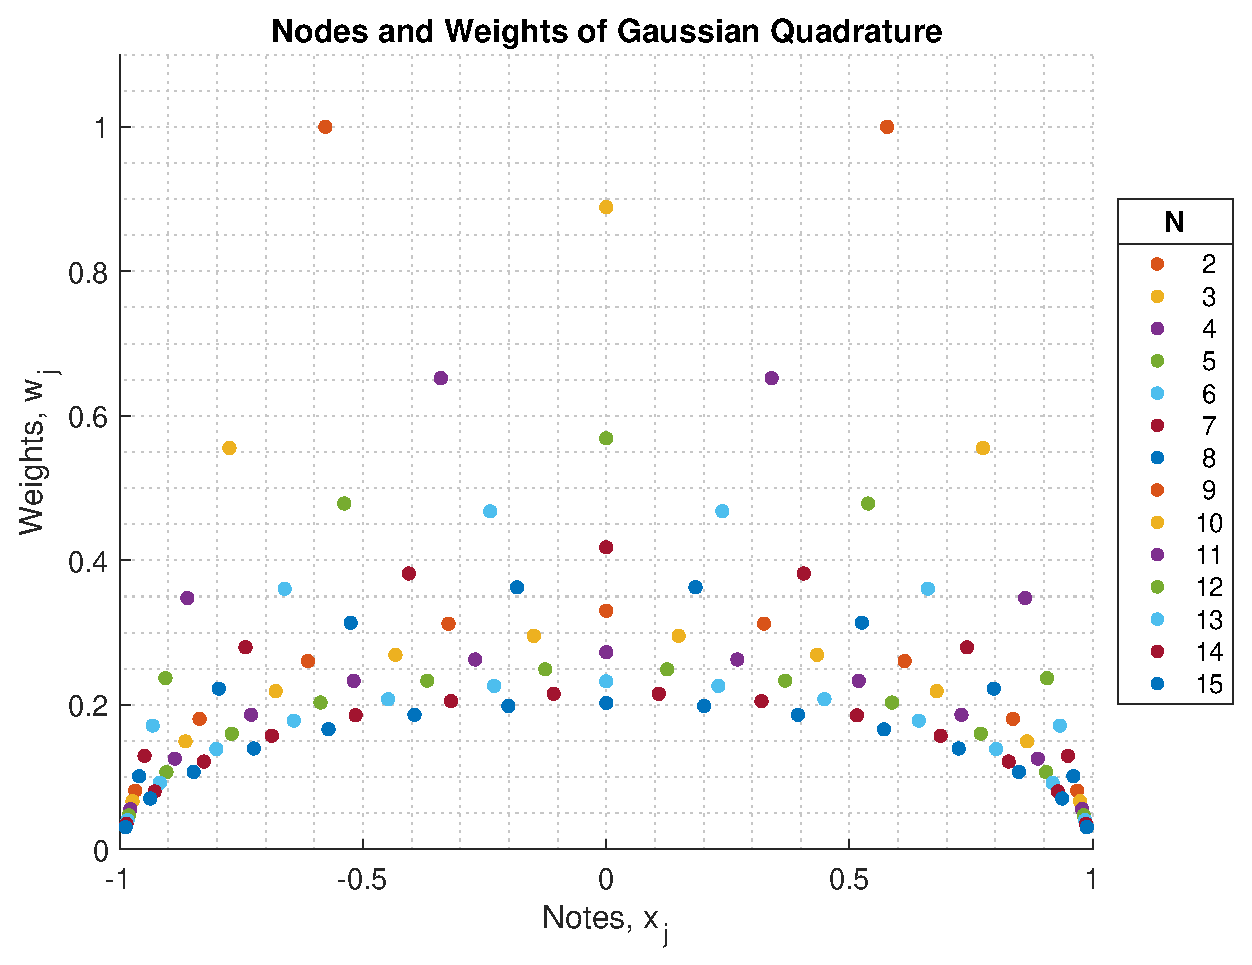
\includegraphics[width=4in]{FastMultipoleMethod/Figures/gaussquad} 
   \caption{Notes and weights of Gaussian quadrature}
   \label{}
\end{figure}

\clearpage
\addtocontents{toc}{\protect\setcounter{tocdepth}{1}}
\subsection{Numerical Integration of Spherical Harmonics}
\addtocontents{toc}{\protect\setcounter{tocdepth}{2}}

Here we derive the number of sampling points needed to numerically integrate spherical harmonics, which follows the results in \cite{darve2000fast}.  Let $f(\theta,\phi)$ be a spherical scalar function composed of a finite number of spherical harmonics
\eq{f(\theta,\phi) = \sum_{l=0}^{L}\sum_{m=-l}^l f_{lm} Y_{lm}(\theta,\phi) \label{fexpansion}}

Integrating this over the unit sphere and separating variables
\ea{\int_0^{2\pi} \int_0^{\pi} f(\theta,\phi) \sin\theta d\theta d\phi  %&=& \sum_{l=0}^{L}\sum_{m=-l}^l f_{lm}  \int_0^{2\pi} \int_0^{\pi} Y_{lm}(\theta,\phi)\sin\theta d\theta d\phi \\
\ & = &  \dfrac{1}{\sqrt{2\pi}}  \sum_{l=0}^{L}\sum_{m=-l}^l  f_{lm}\int_0^{2\pi} e^{im\phi} d\phi \int_0^{\pi}\widetilde P_l^m(\cos\theta) \sin\theta d\theta d\phi \\ }

The integral over $\phi$ can be computed analytically as
\eq{ \int_0^{2\pi} e^{im\phi} d\phi = \begin{cases}
2\pi, \quad \quad m = 0 \\
\dfrac{i (1- e^{2 i \pi m})}{m} = 0, \quad \quad m \ne 0
\end{cases} \label{intphiana} }

It is clear that when $m\ne0$, the double integral will be zero regardless of the value of the $\theta$ integral. We still want to know the number of discrete integration points in $\phi$ required to make this true.  Using trapezoidal integration with periodicity, \eqref{intphiana} is written as a discrete sum over $N$ evenly spaced points
\ea{\int_0^{2\pi} e^{im\phi} d\phi  &=& \Delta \phi \sum_{k=0}^{N-1} e^{im\phi_k}  \\
\ &= & \dfrac{2\pi}{N}  \sum_{k=1}^{N} e^{im k 2\pi/N} \\
\ &= & \dfrac{2\pi}{N}  e^{i(N-1) m \pi/N } \dfrac{\sin(m\pi)}{\sin(m\pi/N)} \label{trapintphi}}

\noindent where $\phi_k = (k-1) \Delta\phi$, $k = 1,...,N$, and $\Delta \phi = 2\pi/N$, The last equation comes from the Dirichlet kernel
\eq{\sum_{k=0}^{N-1} e^{ikx} = e^{i(N-1)x/2} \dfrac{\sin(Nx/2)}{\sin(x/2)}}

\eqref{trapintphi} will be zero when $\vert m \vert < N$, because the numerator sine is zero. When $m = N$, applying L'Hopital's rule, the ratio of sine functions is equal to $N$ while the complex exponent is non-zero. Therefore, the number of samples that correctly integrates all harmonics up to $m = L$ is $N = L + 1$. This can be confirmed numerically and is the same as given in \cite{darve2000fast, beentjes2015quadrature}. We can then write the $\phi$ integral as 
\eq{ \int_0^{2\pi} e^{im\phi} d\phi = \dfrac{2\pi}{L+1} \sum_{i=1}^{L+1} e^{im\phi_i}, \quad 0 \le \vert m \vert \le L }

When $m=0$, the $\theta$ integral becomes 
\ea{ \int_0^{\pi}  P_l(\cos\theta) \sin\theta d\theta &=& - \int_0^{\pi}  P_l(\cos\theta) d\cos\theta \\
\ &=& \int_{-1}^{1}  P_l(\mu) d \mu \\
\ &=& \sum_{j=1}^{N} w_j  P_l(\mu_j) }

with the change of variables $\mu = \cos\theta$ and where the integral has been replaced with Gaussian quadrature. Because $P_l(\mu)$ are polynomials of degree $l$, and because the quadrature is exact for polynomial degrees less than $2n-1$, the number of points that will correctly integrate this is $ l  < 2 n - 1$. For maximum harmonic degree $L$, the number of quadrature nodes is $N = (L+1)/2$, which should be rounded up.  
	
As an aside, when $m$ is even, the associated Legendre polynomials can be integrated with quadrature, because they are simple polynomials. When $m$ is odd, they contain a factor of $\sqrt{1-\mu^2}$, which means they are not simple polynomials, and so cannot be integrated exactly via quadrature. This can be verified numerically. However, analytical integration of $P_l^m(\mu)$ can be done for any $m$, \cite{beentjes2015quadrature,atkinson2012spherical}.


Using these results, numerical integration of a spherical function composed of spherical harmonics with maximum degree $L$ can be computed exactly (to machine precision) as 
\eq{\int_0^{2\pi} \int_0^{\pi} f(\theta,\phi) \sin\theta d\theta d\phi  =   \dfrac{2\pi}{L+1} \sum_{i=1}^{L+1} \sum_{j=1}^{\lceil (L+1)/2 \rceil} w_j f(\theta_j,\phi_i) \label{intsphereharm} }

\noindent where $\phi_i = (i-1)2\pi/(L+1)$, $i = 1,...,L+1$, and $\theta_j = \arccos\mu_j$, where $\mu_j$ and $w_j$ are the nodes and weights of Gaussian quadrature for $\lceil (L+1)/2 \rceil$ points.  

We know that the spherical harmonics are zero-mean over the sphere except the monopole, therefore, if the expansion coefficients are known, one can simply use $f_{00}$ for the mean. If the coefficients are not known, but the function is sampled on the points of quadrature, \eqref{intsphereharm} will compute the mean of $f(\theta,\phi)$ exactly.  

\addtocontents{toc}{\protect\setcounter{tocdepth}{1}}
\subsection{Numerical Integration of Products of Spherical Harmonics}
\addtocontents{toc}{\protect\setcounter{tocdepth}{2}}

Here we derive the number of sampling points needed to numerically integrate a product of spherical harmonics over the unit sphere. This can be done using spherical harmonic synthesis. The expansion coefficients of a scalar spherical function are given by 
\eq{f_{lm} = \int_0^{2\pi} \int_0^{\pi} f(\theta,\phi) Y^*_{lm}(\theta,\phi)\sin\theta d\theta d\phi  }

Substituting \eqref{fexpansion} (ignore for the moment equivalency and orthogonality)
\ea{f_{lm} %&=& \sum_{l'=0}^{L}\sum_{m'=-l'}^{l'} f_{l'm'} \int_0^{2\pi} \int_0^{\pi}  Y_{l'm'}(\theta,\phi)Y^*_{lm}(\theta,\phi)\sin\theta d\theta d\phi \\
&=& \sum_{l'=0}^{L}\sum_{m'=-l'}^{l'} f_{l'm'} \dfrac{1}{2\pi}\int_0^{2\pi} e^{i(m'-m)\phi} d \phi \int_0^{\pi}  \widetilde P_{l'}^{m'}(\cos\theta)  \widetilde P_l^m(\cos\theta)  \sin\theta d\theta \\
 }

Using the reasoning in the previous section, the maximum harmonic in the $\phi$ integration is $2L$. Therefore the number of equally spaced sampling points that are required for trapezoidal integration in $\phi$ is $2L + 1$. The product of two associated Legendre polynomials is a pure polynomial of degree $2L$ for any $m$. Therefore, the number of required samples for Gaussian quadrature in $\theta$ is $\lceil L + 1/2 \rceil$, which can be immediately rounded up to $L + 1$. 

Using these, numerical integration of the product of two spherical 
functions, $f(\theta,\phi)$ and $g(\theta,\phi)$, each with maximum harmonic degree $L$ can be computed exactly as 
\eq{\int_0^{2\pi} \int_0^{\pi} f(\theta,\phi) g(\theta,\phi)  \sin\theta d\theta d\phi =  \dfrac{2\pi}{2L+1} \sum_{i=1}^{2L+1} \sum_{j=1}^{L+1} w_j f(\theta_j,\phi_i)g(\theta_j,\phi_i) \label{intharmprod}}

\noindent where $\phi_i = (i-1)2\pi/(2L+1)$, $i = 1,...,2L+1$, and $\theta_j = \arccos\mu_j$, where $\mu_j$ and $w_j$ are the nodes and weights of Gaussian quadrature for $L + 1$ points.  It is common to find \eqref{intharmprod} in the literature applied to spherical functions without stipulating whether the underlying function is composed of pure harmonics of a product of spherical harmonics.


 \begin{figure}[H] 
   \centering
   \subfigure{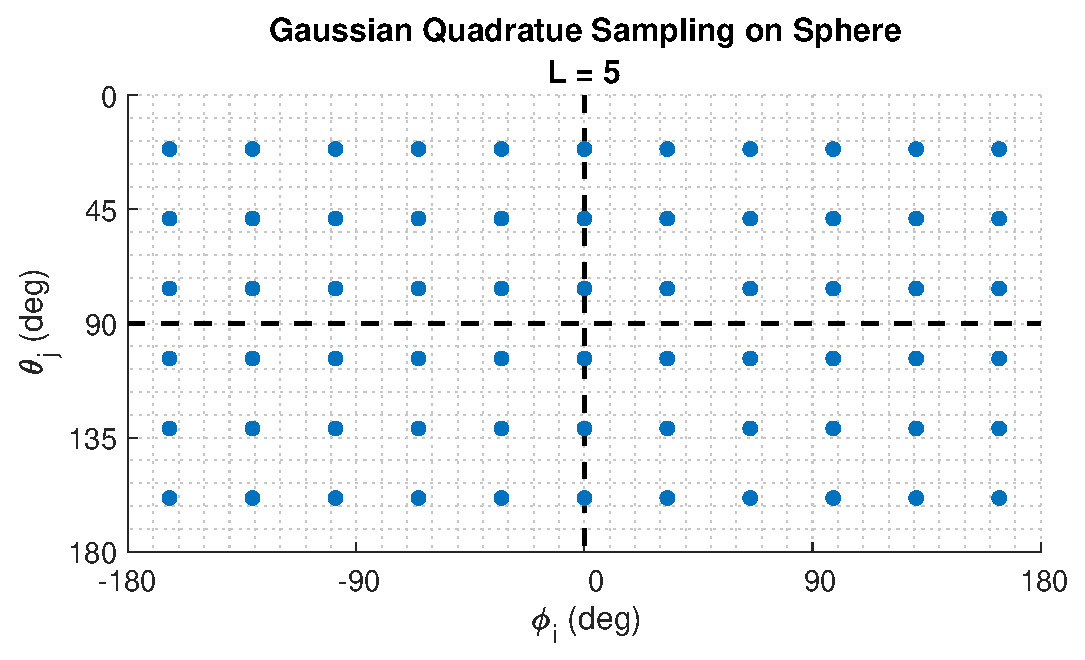
\includegraphics[width=3in]{FastMultipoleMethod/Figures/quadsphere5}}
       \subfigure{\includegraphics[width=3in]{FastMultipoleMethod/Figures/quadsphere6}}
   \caption{Nodes of trapezoidal integration ($\phi_i$) and Gaussian quadrature ($\theta_j$) for integrating products of spherical functions.}
   \label{}
\end{figure}



The nodes $\theta_j$ are almost uniformly spaced, and they never sample the poles because of the nodes of Gaussian quadrature do not sample the end points. This is especially convenient for vector spherical harmonics where the polarization is ambiguous at the poles. When $L+1$ is odd, the nodes will sample the equator. This scheme does crowd the poles somewhat.

Finally, \eqref{intharmprod} can be viewed as computing the power of a field over the sphere when the second function is conjugated (or computing the cross-correlation of two fields). If the spherical harmonic expansion coefficients are known, the analogous form of Parseval's theorem can be used to simply sum the magnitude squared of the coefficients. If the coefficients are not known, \eqref{intharmprod} will compute a power-like quantity exactly from samples of the field(s). 



%
%Integration of a spherical function $f(\hat{\bb{k}})$ over the unit sphere can be written generally as 
%\eq{\int f(\hat{\bb{k}}) d\hat{\bb{k}} = \int_0^{2\pi} \int_0^{\pi} f(\theta,\phi) \sin\theta d\theta d\phi }
%
%\noindent where $\hat{\bb{k}} = (\sin\theta\cos\phi, \sin\theta\sin\phi, \cos\theta)$.  
%
%This integral can be computed exactly from the samples of $f(\hat{\bb{k}})$, if $f$ is band-limited, using a hybrid of Gauss-Legendre quadrature in $\theta$ and trapezoidal integration in $\phi$.  After a change of variables, the integral is 
%\begin{eqnarray}
%\int f(\hat{\bb{k}}) d\hat{\bb{k}} & =& \int_0^{2\pi} \int_0^{\pi} f(\theta,\phi) \sin\theta d\theta d\phi \\
%\ & =& \int_0^{2\pi} \int_{-1}^1 f(\mu,\phi) d\mu d\phi \\
%\ & = & \dfrac{2\pi}{2L+1} \sum_{i=1}^{2L+1} \sum_{j=1}^{L+1} w_j f(\theta_j,\phi_i) \label{sphereint}
%\end{eqnarray}
%
%
%
%
%\noindent where $w_j$ are the weights corresponding to Gaussian nodes $\mu_j$ on $[-1,1]$. The angular sampling points are $\theta_j = \arccos\mu_j$ and $\phi_i = (i-1)2\pi/(2L+1)$. $L$ is the maximum degree required to expand the function $f(\theta,\phi)$ in spherical harmonics.  Interestingly, the nodes $\theta_j$ are almost uniformly spaced, and they never sample the poles because of the nodes of Gaussian quadrature do not sample the end points. When $L+1$ is odd, the nodes will sample the equator.
%
%Address the no-quite polynomials for straight spherical harmonics.   Spherical transforms and green's function contain products of these harmonics. 

\addtocontents{toc}{\protect\setcounter{tocdepth}{1}}
\subsection{Green's Function Integration}
\addtocontents{toc}{\protect\setcounter{tocdepth}{2}}

Following \cite{yucel2008helmholtz}, we give the number of sample points required to correctly integrate the plane wave expansions in the FMM. Using the addition theorem for plane waves 
\eq{e^{i \bb{k}\cdot \bb{d}} = \sum_{l=0}^{\infty} i^l (2l+1) j_l(kd) P_l(\hat{\bb{k}}\cdot\hat{\bb{d}})}

\eqref{fmmexp3} can be written 
\ea{\dfrac{e^{ik\vert \bb{X} + \bb{d} \vert}}{\vert \bb{X} + \bb{d} \vert}  &=& \dfrac{i k}{4\pi}  \sum_{l=0}^{\infty} \sum_{l'=0}^{\infty} i^l (2l+1) i^{l'} (2l'+1) h_l^{(1)}(k X)   j_l'(kd)   \int   P_l(\hat{\bb{k}} \cdot\hat{\bb{X}}) P_l'(\hat{\bb{k}}\cdot\hat{\bb{d}})   d\Omega_k }

Using the addition theorem for Legendre polynomials, 
\eq{P_l(\hat{\br} \cdot \hat{\br}') = \dfrac{4\pi}{2l + 1} \sum_{m=-l}^l Y_{lm}(\theta,\phi) Y_{lm}^*(\theta',\phi')}

the integral can be expanded as 
\eq{\int  P_l(\hat{\bb{k}} \cdot\hat{\bb{X}}) P_l'(\hat{\bb{k}}\cdot\hat{\bb{d}})   d\Omega_k   = \dfrac{4\pi}{2l + 1} \dfrac{4\pi}{2l' + 1}  \sum_{m=-l}^l  \sum_{m=-l'}^{l'} Y_{lm}^*(\theta_X',\phi_X') Y_{lm}^*(\theta_d',\phi_d')    \int  \left(Y_{lm}(\theta_k,\phi_k)\right)^2 d\Omega_k }

Which shows that the spherical integral in \eqref{fmmexp3} is really integrating a product of spherical harmonics. Therefore, using the results from the previous section, the integral over planes waves in the Green's function kernel \eqref{kernelexp} can be computed exactly over discrete values of the wave vector $\hat{\bb{k}}_{ij}$ as 
\eq{ \dfrac{e^{ik\vert \br - \br' \vert}}{\vert \br - \br' \vert}  \approx \dfrac{ik}{4\pi} \dfrac{2\pi}{2L+1} \sum_{i=1}^{2L+1} \sum_{j=1}^{L+1} w_j  e^{ik \hat{\bb{k}}_{ij}\cdot(\br - \br_o)} T_L(k \hat{\bb{k}}_{ij},\bb{X}) e^{-ik \hat{\bb{k}}_{ij} \cdot(\br' - \br_s) } }

which is the result in \cite{yucel2008helmholtz}. The approximation comes from truncating the sum in \eqref{kernelexp}, not the spherical integration.  




\section{Aggregation/Disaggregation}

Here we give a basic idea of how to aggregate, translate, and disaggregate fields in the context of the FMM operations following the explanation in \cite{yucel2008helmholtz}. The routines for computing the translation operator are given in Section \ref{transoperator}, while routines for interpolating and filtering scalar and vector fields are given in Sections \ref{sec:scasphfilter} and \ref{sec:vecsphfilter}.

\addtocontents{toc}{\protect\setcounter{tocdepth}{1}}
\subsection{Octree}
\addtocontents{toc}{\protect\setcounter{tocdepth}{2}}

Typically the scatterers in an FMM problem are organized on a hierarchical octree. An octree is a data structure in which each node has eight children. This is combined with the geometric process of subdividing a cubic volume into eight equal octants. The eight subcubes are called the children of the larger parent cube and visa versa. A cube at every level has an outgoing and incoming far-field pattern associated with it, say $\bb{F}(\hat {\bb{k}})$, which is sampled on the sphere according to the rules of quadrature. This field expansion is centered on the cube and has harmonic bandwidth (i.e., maximum degree vector spherical harmonic, $L$) at least as large as that required for the diameter of the enclosing sphere, and further set by the desired accuracy of the translation operations. This means that fields are coarsely sampled in $(\theta,\phi)$ at higher levels (smaller cubes), and more finely sampled at lower (larger cubes) levels.

Fields are aggregated up the hierarchy, translated at the highest level possible, then disaggregated down the hierarchy. There is a constraint that fields cannot be translated to neighboring boxes at the same level (due to the separation requirement of the translation). This creates a complication when disaggregating. For more details see \cite{yucel2008helmholtz}. In general, aggregation and disaggregation do not have to be restricted to octree structures as long as the bandwidth and separation between the groups of scatterers is obeyed. 


 \begin{figure}[h] 
   \centering
   \includegraphics[width=6in]{FastMultipoleMethod/Figures/aggdiss} 
   \caption{Aggregation, translation, and disaggregation. }
   \label{}
\end{figure}



\addtocontents{toc}{\protect\setcounter{tocdepth}{1}}
\subsection{Aggregation}
\addtocontents{toc}{\protect\setcounter{tocdepth}{2}}

To reiterate, the far pattern of each child cube has lower harmonic content than the parent (due to its smaller size), and therefore coarser spatial sampling in $(\theta,\phi)$. The process of aggregating fields consists of 1) interpolating each far pattern of the children cubes up to the finer sampling of the parent, 2) shifting the phase centers of the children's patterns to that of the parent, then 3) summing the fields of the all the children. The shift is done by multiplication by a complex exponential of plane wave phases, which is equivalent to a diagonal matrix-vector multiply and is trivial to compute. 

Let $\bb{F}_{n,l}(\hat {\bb{k}})$ be the vector field for the $n$th group (cube) at level $l$.  Let $P_{l+1}^{l}$ be the interpolation operator that interpolates a field from level $l+1$ to level $l$. The aggregated field for the $n$th group at the level of the parents is the sum over all interpolated and shifted fields of the children belonging to each parent, \cite{yucel2008helmholtz}:
\begin{equation}
\bb{F}_{n,l}(\hat {\bb{k}}_{l}) = \sum_{m \in G_c} e^{i\bb{k}_{l+1} \cdot (\bb{x}_{n} - \bb{x}_{m}) } P_{l+1}^{l}\left[\bb{F}_{m,l+1}(\hat{ \bb{k}}_{l+1})\right]
\end{equation}

\noindent where $G_c$ are the list of children that belong to parent group $n$, and $\hat {\bb{k}}_{l}$ are the spherical directions sampled for level $l$.

The process of interpolation does not change the harmonic content of the patterns of the children. However, multiplying the pattern by the phase exponential of the plane wave shift is equivalent to convolving the spherical harmonic spectra. This is why the fields are first interpolated, then translated. Another way to think about this is, even though the patterns of the children may contain lower harmonic content when centered on the cubes of the children, the same pattern that is offset from a different center, now belongs to a larger enclosing sphere, and therefore has more harmonic content requiring finer spherical sampling.

\addtocontents{toc}{\protect\setcounter{tocdepth}{1}}
\subsection{Disaggregation}
\addtocontents{toc}{\protect\setcounter{tocdepth}{2}}

Disaggregation sweeps from the lowest level of the octree (largest cubes) to the highest level (smallest cubes) and consists of three steps: 1) shift the field of a parent to the phase center of the child then filter the parent's field to the child's level (i.e., anterpolate), 2) translate the outgoing patterns between groups at the same level that are not near-neighbors but whose parents are near-neighbors (i.e., called the neighborhood of the child), 3) sum the filtered and translated fields. This is done recursively from the bottom level to the top level for all groups and can be written. 
\begin{equation}
\bb{G}_{m,l}(\hat {\bb{k}}_{l}) = P_{l-1}^{l}\left[e^{i\bb{k}_{l-1} \cdot (\bb{x}_{m} - \bb{x}_{n}) }  \bb{G}_{n,l-1}(\hat{ \bb{k}}_{l-1})\right] + \sum_{p \in G_w} T_L({\bb{k}}_{l}, \bb{x}_{m} - \bb{x}_{p}) \bb{F}_{p,l}(\hat {\bb{k}})
\end{equation}

\noindent where $P_{l-1}^{l}$ is the filtering operator that filters the parent's field at level $l-1$ to the child sampling, $m$ is index of the child at level $l$, $n$ is the index of the parent at the parent's level, and $G_w$ is the list children at level $l$ that are well-separated from $m$ (i.e., children that are not near-neighbors, but whose parents are near-neighbors). The purpose of filtering the field of the parent is to reduce its total harmonic content to be of the same degree as that of the child. 


\section{Translation Operator}
\label{transoperator}

\subsection{Basic Translation Operator}
The FMM translation operator is 
\begin{equation}
T_L(\bb{k},\bb{X}) = \sum_{l=0}^L i^l (2l+1) h_l^{(1)} (kX) P_l(\hat{\bb{k}}\cdot\hat{\bb{X}}) 
\end{equation}

\noindent where $\bb{X}$ is the Cartesian vector that points from the origin of the source frame to the origin of the observation frame, $k$ is the complex background wavenumber, $\hat{\bb{k}}$ is the Cartesian wave vector direction, $P_l(x)$ is the Legendre polynomial, and $L$ is the maximum degree of the sum. When computing this, it can be written terms of the dot product $\cos\theta = \hat{\bb{k}}\cdot\hat{\bb{X}}$ in order to externalize the vector computations.
\begin{equation}
T_L(kX,\theta) = \sum_{l=0}^L i^l (2l+1) h_l^{(1)} (kX) P_l(\cos\theta) \label{tltheta}
\end{equation}


 \begin{figure}[h] 
   \centering
   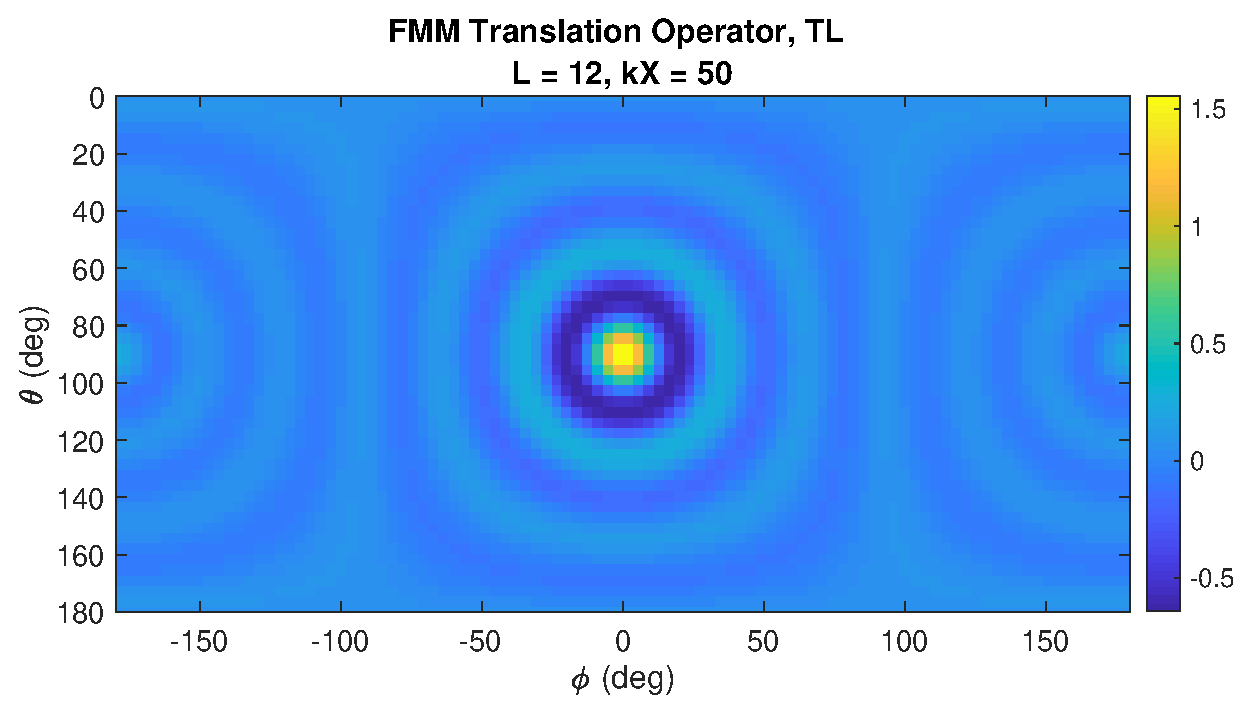
\includegraphics[width=3.5in]{FastMultipoleMethod/Figures/TLtheta} 
   \caption{Real part of the translation operator, \eqref{tltheta}, for $\hat{\bb{X}} = [1, 0, 0]$, $L = 12$, and $kX = 50$. The grid is highly oversampled compared to the sampling required for quadrature integration over the sphere. Note, the operator is peaked in the direction of propagation and contains a 'back lobe'-like feature.}
   \label{}
\end{figure}



The routine \texttt{TLth} returns the translation operator \eqref{tltheta} given scalars $kX$, $L$, and array of $\cos\theta$, which can be any size. To save memory, the Legendre polynomials are computed inline with the recursion \eqref{plrec}.

{\footnotesize
\VerbatimInput{\code/FastMultipoleMethod/TL/TLth.m}
}



%
%
%
%{\footnotesize
%\VerbatimInput{\code/FastMultipoleMethod/TLth.m}
%}
%
%{\footnotesize
%\VerbatimInput{\code/FastMultipoleMethod/TLmem.m}
%}

\subsection{Translation Operator Interpolation}

Computing the translation operator as a straight sum is a computational bottleneck for large problems.  Much work has gone into finding an optimal computation scheme, and the result is a fast interpolator.  The translation operator is precomputed directly at a coarse sampling, after which any value is found by interpolation to a selectable level of error.  Because the translation operator is band limited, it can be computed exactly from the samples using the approximate prolate spheroid (APS) method.  In practice, only a small subset of samples in the vicinity of the interpolation point needs to be used.  

The interpolation formula using APS is given by \cite{bucci1991optimal,yucel2008helmholtz}
\begin{equation}
\widetilde{T}_L(\theta) = \sum_{m = m_o - p + 1}^{m_o + p} T_L(m\Delta\theta)S_N(\theta-m\Delta\theta,\theta_o)D_M(\theta - m \Delta\theta)
\end{equation}

\noindent where $\widetilde{T}_L(\theta)$ is the interpolated translation operator, $D_M(\theta)$ is the periodic sinc function (or Dirichlet kernel), $S_N(\theta,\theta_o)$ is a windowing function, and $T_L(m\Delta\theta)$ are precomputed samples of the translation operator.  The windowing function is given by 
\begin{equation}
S_N(\theta,\theta_o) = \dfrac{R_N(\theta,\theta_o)}{R_N(0,\theta_o)} 
\end{equation}
\begin{equation}
R_N(\theta,\theta_o) = \dfrac{\sinh\left[ (2N+1) \sinh^{-1} \sqrt{\sin^2(\theta_o/2) - \sin^2(\theta/2)}\right]}{\sqrt{\sin^2(\theta_o/2) - \sin^2(\theta/2)}}
\end{equation}

The Dirichlet kernel is given by 
\begin{equation}
D_M(\theta) = \dfrac{\sin\left[(2M+1)\theta/2 \right]}{(2M+1)\sin(\theta/2)}
\end{equation}

In these expressions, $L$ is the truncation degree of the sum and $M=sL$ is the total number of precomputed sampling points where $s$ is the over-sampling ratio and is an integer.  The required sample spacing is $\Delta \theta = 2\pi/(2M+1)$.  This spacing is over a $2\pi$ circumference, even though we only need $\theta = [0, \pi]$.  This comes from the original papers on optimal interpolation over a sphere, but the formulation persists in the literature.  $N = M-L = (s-1)L$ is the number of over-sampling points.  $m_o = \textrm{Int}[\theta/\Delta\theta]$ is the integer index to the left of the interpolation point, where $\textrm{Int}[\cdot]$ is the integer part or floor function.   $\theta_o = p\Delta\theta$ is the width of the interpolation window, where $p$ is the number of samples on each side of the interpolation point.  The choice of $s$ and $p$ is important for maintaining accuracy while minimizing computation.  Good empirical values are $s = 5$, $p= 3$.  

 \begin{figure}[H] 
   \centering
   \includegraphics[width=3in]{FastMultipoleMethod/Figures/indexing} 
   \caption{Sampling and indexing of the interpolation.  Example for $M = 8$, $p = 3$.  $m=0$ corresponds to $\theta = 0$. Note no sample at $\theta=\pi$.}
   \label{fig4}
\end{figure}

Even though we will only interpolate $\theta = [0, \pi]$, we require precomputed samples outside this range when interpolating near the ends.  The translation operator is an even function of $\theta$, therefore, there are two options to obtain the out of bounds points: 1) Only compute sampling points in the range $\theta = [0, \pi]$ and loop the summation index $m$ back on itself if we go beyond the ends, or 2) precompute the necessary values outside of the range, and let the index roam free. We choose the first for simplicity.  

Figure \ref{fig4} illustrates the sample spacing as it relates to the number of sample points as well as the indexing scheme for precomputing points outside the range $\theta = [0, \pi]$.  There are $p-1$ samples to the left of 0, $p$ samples after $\pi$, $M + 2p$ total sample points, and the array index is $I = m + p$, where $m = [0,M]$.  Figure \ref{fig5} shows the interpolator.  

 \begin{figure}[H] 
   \centering
   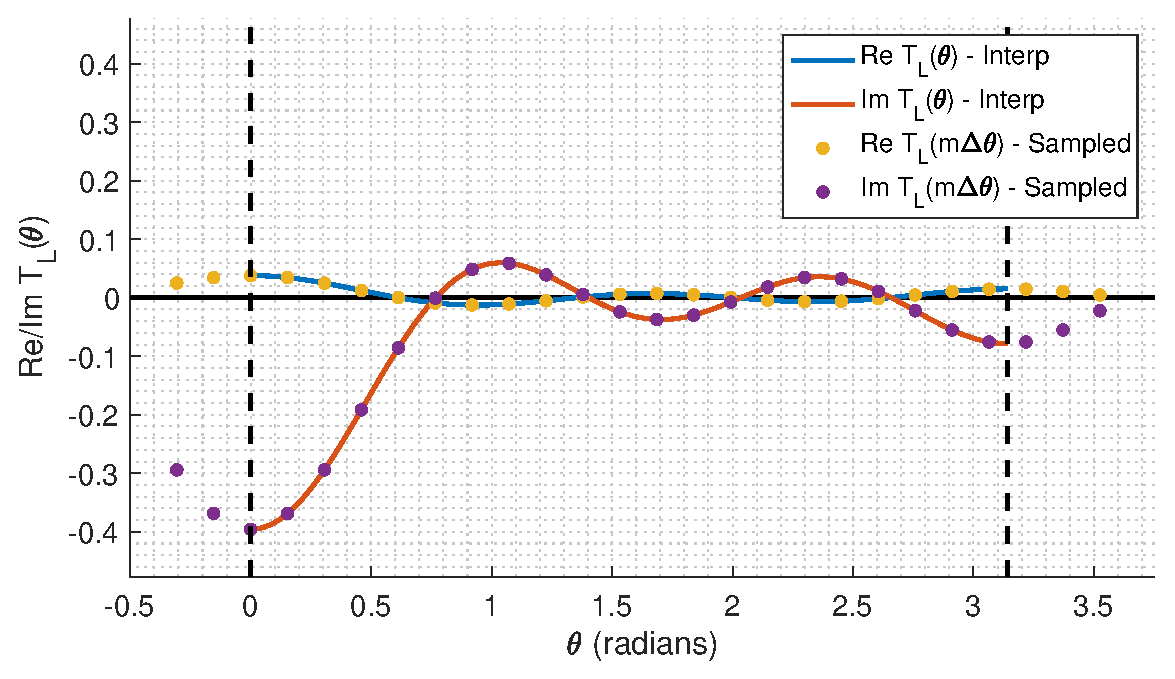
\includegraphics[width=4in]{FastMultipoleMethod/Figures/TLthetainterp} 
   \caption{Translation operator interpolator.  $L = 4$, $s = 5$, $p = 3$, $M = 20$ and there are $M + 2p$ total sampling points.  $k = 2\pi$, $r = 10$. Note there is no sampling point at $\theta = \pi$.}
   \label{fig5}
\end{figure}

The routine \texttt{interpTL} takes as inputs the outputs from the preparatory function \texttt{interpTLprep} as well as the interpolation point(s).  The helper functions are the windowing and Dirichlet kernel, \texttt{SN} and \texttt{DM}.  


{\footnotesize
\VerbatimInput{\code/FastMultipoleMethod/TL/interpTL.m}
}

{\footnotesize
\VerbatimInput{\code/FastMultipoleMethod/TL/interpTLprep.m}
}

{\footnotesize
\VerbatimInput{\code/FastMultipoleMethod/TL/SN.m}
}

{\footnotesize
\VerbatimInput{\code/FastMultipoleMethod/TL/DM.m}
}




\section{Scalar Spherical Filter}
\label{sec:scasphfilter}

In this section, we give routines for interpolating and filtering scalar spherical harmonics following \cite{yucel2008helmholtz}. These routines can stand on their own, because they are excellent for general applications of spherical harmonic expansions. The scalar filters can be used in the scalar form of the FMM for interpolating and filtering fields up and down the multi-level hierarchy structure. These lay the ground work for the vector spherical filters derived later.

\subsection{Spherical Harmonic Transforms}

The spherical harmonics form a complete basis, so any band-limited spherical signal can be represented as a finite sum of harmonics
\begin{equation}
f(\theta,\phi) = \sum_{l=0}^{L} \sum_{m = -l}^{l} f_{lm} Y_{lm}(\theta,\phi)
\label{c6eq1}
\end{equation}

Spherical harmonics can be written in terms of the normalized Legendre polynomials as 
\begin{equation}
Y_{lm}(\theta,\phi) = \dfrac{1}{\sqrt{2\pi}}\widetilde{P}_l^m(\cos \theta)e^{im\phi}
\end{equation}

Using orthogonality of the spherical harmonics, the expansion coefficients are

%\begin{equation}
%\int_{0}^{2\pi} \int_{0}^{\pi} Y_{lm}(\theta,\phi) Y^*_{l'm'}(\theta,\phi) \sin\theta d\theta d\phi = \delta_{ll'}\delta_{mm'}
%\end{equation}

%from which is follows that

\begin{equation}
f_{lm} = \int_{0}^{2\pi} \int_{0}^{\pi}  f(\theta,\phi) Y^*_{l'm'}(\theta,\phi) \sin\theta d\theta d\phi   
\label{c6eq3}
\end{equation}

Equation \eqref{c6eq3} is the forward transform, or spherical harmonic analysis, while equation \eqref{c6eq1} is the inverse transform, or spherical harmonic synthesis.  




\subsection{Forward Scalar Spherical Transform}

Computing \eqref{c6eq3} consists of two steps: 1) forward Fourier transform in $\phi$, 2) forward Legendre transform in $\theta$.  Writing out \eqref{c6eq3}
\begin{equation}
f_{lm} = \int_{0}^{\pi} \widetilde{P}_l^m(\cos \theta) \sin \theta d \theta \dfrac{1}{\sqrt{2\pi}} \int_{0}^{2\pi}   f(\theta,\phi) e^{-im\phi} d\phi   
\end{equation}

\noindent where $\widetilde{P}_l^m(\cos \theta)$ are the fully normalized Legendre polynomials.  The $\phi$ integral is computed first in order to create a set of 1D functions of $\theta$ for each $m$
\begin{equation}
f_m(\theta) = \dfrac{1}{\sqrt{2\pi}} \int_{0}^{2\pi}   f(\theta,\phi) e^{-im\phi} d\phi   
\end{equation}

Evaluating this with trapezoidal integration
\begin{equation}
f_m(\theta) = \dfrac{\sqrt{2\pi}}{I} \sum_{i=1}^{I} f(\theta,\phi_i) e^{-im\phi_i} 
\end{equation}

\noindent where $I$ is the number of grid points in longitude and $\phi_i = 2\pi i/ I $ for $ i = 0,...,I-1$.  This can be computed via FFT. The $\theta$ integral is next computed for each $f_m(\theta)$ by using the forward Legendre transform with a change of variables 
\ea{f_{lm} &=& \int_{0}^{\pi} f_m(\theta) \widetilde{P}_l^m(\cos \theta) \sin \theta d \theta \\
\ & = & -\int_{0}^{\pi} f_m(\theta) \widetilde{P}_l^m(\cos \theta) d\cos\theta \\
\ & = & \int_{-1}^{1} f_m(\theta( \mu)) \widetilde{P}_l^m(\mu) d\mu, \quad \mu = \cos\theta }

%
%\begin{equation}
%f_{lm} = \int_{0}^{\pi} f_m(\theta) \widetilde{P}_l^m(\cos \theta) \sin \theta d \theta 
%\end{equation}
%
%Making a change of variables
%\begin{eqnarray}
%%f_{lm} &=& \int_{0}^{\pi} f_m(\theta) \widetilde{P}_l^m(\cos \theta) \sin \theta d \theta \\
%f_{lm} & = & -\int_{0}^{\pi} f_m(\theta) \widetilde{P}_l^m(\cos \theta) d\cos\theta \\
%%\ & = & \int_{\pi}^{0} f_m(\theta) \widetilde{P}_l^m(\cos \theta) d\cos\theta \\
%\ & = & \int_{-1}^{1} f_m(\theta( \mu)) \widetilde{P}_l^m(\mu) d\mu, \quad \mu = \cos\theta 
%\end{eqnarray}

This can now be evaluated with Gaussian quadrature on the interval $\mu = [-1, 1]$ as
\begin{equation}
f_{lm} = \sum_{j=1}^J f_m(\theta_j) \widetilde{P}_l^m(\mu_j) w_j \label{forwardlegendre}
\end{equation}

\noindent where $J$ is the number of points in latitude and the weights, $w_j$, correspond to the nodes $\theta_j = \arccos\mu_j$.  One first selects the number of grid points in latitude, retrieves the Gaussian nodes for that number of integration points, then evaluates the points $\theta_j$.  Because this operation is integrating products of spherical harmonics, the integral is exact if the number of grid points in latitude and longitude are $J = L+1$ and $I = 2L+1$ for coefficients through $L$. By virtue of the Gaussian quadrature node spacing, the field is never evaluated at the poles.

The routine \texttt{sst} performs the forward scalar spherical transform and returns the spectral coefficients $f_{lm}$.  The coefficients are returned on a 1D array of size $L^2 + 2L + 1$, linearly indexed.  It takes as inputs the maximum degree $L$ for which harmonics are desired. The spherical function $f(\theta_j,\phi_i)$ is sampled on an $I \times J$ meshgrid, where $I = 2L'+1$ and $J = L'+1$ are such that $L' \ge L$.  The sample points need to be $\phi_i = 2\pi i/ I $ for $ i = 0,...,I-1$, and $\theta_j = \arccos \mu_j $, where $\mu_j$ are the $J$ quadrature nodes on $\mu = [-1, 1]$, which are also inputs. In other words, the grid can be sampled more finely than the maximum degree of the harmonics desired for the coefficients. $f_m(\theta_j)$ is computed in place with an FFT along the first dimension of the array.  Matlab's \texttt{fft} produces a two-sided DFT, and $2L+1$ is always odd, so the rows of the matrix $f_m(\theta_j)$ correspond to the spectral components $m = 0, 1, ..., (I-1)/2, -(I-1)/2, ..., -1$.  The rows of the 1D FFT are indexed 
\begin{equation}
\textrm{idx}(I,m) = \left\{ \begin{array}{cc} m + 1, & m \ge 0 \\ I - m + 1, & m < 0 \\ \end{array} \right.
\end{equation}

%Finally, this uses our routine \texttt{Plm} for associated Legendre polynomials, which ensures that one factor of $(-1)^m$ in included in the definition of the spherical harmonics.


%uses onThe Legendre polynomials are computed normalized with Matlab's \texttt{legendre} function and \texttt{'norm'} option.  An extra factor of $(-1)^m$ is included in that definition. Therefore, we need to cancel this to be content with our use of the Condon-Shortly phase that we include in our definition of spherical harmonics.

%
%Note: the definition of Legendre polynomials has a factor of $(-1)^m$.  Our definition of spherical harmonics includes the Condon-Shortly phase, which means there are really two factors of $(-1)^m$ in the entire definition.  Our spherical harmonics are consistent with the wave function translation matrices.  This derivation of the filter does not include the extra $(-1)^m$ on the spherical harmonics, only the one in the definition of the Legendre polynomials, which is also included with the \texttt{'norm'} option.  The filter works was shown to work with just the one factor.  Therefore, we take out the second factor of $(-1)^m$ by multiplying by $(-1)^m$.  If the definition of the the spherical harmonics does not include that phase, then that part of the code should be removed.

{\footnotesize
\VerbatimInput{\code/FastMultipoleMethod/SphericalFilters/sst.m}
}



\subsection{Inverse Scalar Spherical Transform}

The inverse transform consists of taking the expansion coefficients $f_{lm}$ and applying 1) the inverse Legendre transform in $\theta$, 2) the inverse Fourier transform in $\phi$.  The inverse Legendre transform is 

\begin{equation}
f_m(\theta_j) = \sum_{l = \vert m \vert}^{L} f_{lm} \widetilde{P}_l^m(\mu_j)
\label{eqist1}
\end{equation}

\noindent where again $\mu_j = \cos\theta_j$.  The inverse Fourier transform in $\phi$ is

\begin{equation}
f(\theta_j,\phi_i) = \dfrac{1}{\sqrt{2\pi}}\sum_{m = -L}^{L} f_m(\theta_j) e^{im\phi_i}
\label{eqist2}
\end{equation}

The routine \texttt{isst} computes the inverse scalar spherical transform.  The inputs are the array of harmonics $f_{lm}$ of size $L^2 + 2L + 1$ linearly indexed, and the maximum degree $L$. It then returns the $I \times J$ spherical function $f(\theta_j,\phi_i)$ as a meshgrid such that $I = 2L'+1$ and $J = L' + 1$, where $\phi_i = 2\pi i/ I $ for $ i = 0,...,I-1$, and $\mu_j = \cos\theta_j$.  $J$ is determined by the length of the input $\mu_j$, which can be larger than the corresponding sampling of the $L$ harmonics in $f_{lm}$ (this allows the routine to preform interpolation automatically). An additional factor of $I$ is needed because Matlab's \texttt{ifft} divides by the number of samples in $\phi$.  

{\footnotesize
\VerbatimInput{\code/FastMultipoleMethod/SphericalFilters/isst.m}
}

\clearpage

\subsection{Scalar Spherical Filter}

The forward and inverse scalar spherical transforms can be used together to accomplish interpolation or filtering (anterpolation) of a spherical function.  

Interpolation takes a function $f(\theta,\phi)$ with coarse sampling and $L$ harmonics, and upsamples it to a function $f(\theta',\phi')$ with finer sampling and $K$ harmonics, where $K > L$.  Because the original signal is band limited with maximum harmonic $L$, the interpolated signal contains the same harmonic content, and is interpolated exactly. This is the spherical harmonic analog of upsampling a Nyquist-sampled exactly to an arbitrarily fine sampling with sinc interpolation.  Interpolation is accomplished by first computing the spectral components $f_{lm}$ of $f(\theta,\phi)$ using the scalar spherical transform to degree $L$, zero-padding the coefficients to degree $K$ to form $f_{lm}'$, then applying the inverse scalar spherical transform to create $f(\theta',\phi')$.

Filtering takes $f(\theta',\phi')$ with fine sampling and $K$ harmonics to a function $f(\theta,\phi)$ with coarse sampling and $L$ harmonics, where $L < K$.  This is analogous to filtering a signal and resampling it at lower rate.  Filtering necessarily eliminates higher frequency harmonics.  Filtering is accomplished by computing the spectral components $f_{lm}'$ of $f(\theta',\phi')$ via the SST to degree $K$, truncating down to degree $L$ to form $f_{lm}$, then applying the ISST to create $f(\theta,\phi)$.

\begin{equation}
\begin{array}{cccccccccc}
\textrm{Interpolation:} & f(\theta,\phi) & \stackrel{\textrm{sst}}{\rightarrow} & f_{lm}, L & \rightarrow & \textrm{zero pad} &\rightarrow & f_{lm}', K & \stackrel{\textrm{isst}}{\rightarrow} & f(\theta',\phi') \nonumber \\
\textrm{Filter:} & f(\theta',\phi') & \stackrel{\textrm{sst}}{\rightarrow} & f_{lm}', K & \rightarrow & \textrm{trunctate} &\rightarrow & f_{lm}, L &\stackrel{\textrm{isst}}{\rightarrow} & f(\theta,\phi) \nonumber \\
\end{array}
\end{equation}

%
% \begin{figure}[h] 
%   \centering
%   \includegraphics[width=3.5in]{FastMultipoleMethod/Figures/samples} 
%   \caption{Sample spacing for $L = 4$.}
%   \label{}
%\end{figure}
%


 \begin{figure}[H] 
 \centering
\subfigure{
\includegraphics[width=3in]{FastMultipoleMethod/Figures/filt1} } 
\subfigure{
\includegraphics[width=3in]{FastMultipoleMethod/Figures/filt2} } 
\caption{Interpolation of a complex scalar field (real part). Left: coarsely sampled field. Right: finely sampled interpolated field. }
\end{figure}

 \begin{figure}[H] 
 \centering
\subfigure{
\includegraphics[width=3in]{FastMultipoleMethod/Figures/filt3} } 
\subfigure{
\includegraphics[width=3in]{FastMultipoleMethod/Figures/filt4} } 
\caption{Filtering of a complex scalar field (real part). Left: finely sampled field. Right: coarsely sampled filtered field. }
\end{figure}


The routine \texttt{ssfilt} computes the scalar spherical interpolation or filtering operation.  It takes the maximum harmonic degrees $L$ and $K$, where $L \le K$.  The harmonic content is either interpolated from $L$ to $K$ or filtered from $K$ to $L$.  For interpolation, the input function is $f(\theta,\phi)$, sized $2L'+1 \times L' + 1$ on a meshgrid, and the routine returns $f(\theta',\phi')$, sized $2K'+1 \times K'+1$, where $L'$ and $K'$ are set by the length of $\mu_j$ and $\mu_k$, respectively.  The sampling of the grid can have more harmonics than the interpolation/filter harmonics. As always, it assumes $\phi$ is uniformly spaced and $\theta$ is spaced according to the Gaussian quadrature nodes.  This routine calls \texttt{sst} and \texttt{isst} that recompute the underlying Legendre polynomials at each run and is not built for speed.  

{\footnotesize
\VerbatimInput{\code/FastMultipoleMethod/SphericalFilters/ssfilt.m}
}

\clearpage

\subsection{Fast Scalar Spherical Filter}
\label{sec:fastscasphfilt}
The bottle neck of the scalar spherical filter lies in the sums of the forward and inverse Legendre transforms, especially when $L$ is large.  The fix is to combine the two transforms, after which the sums can be simplified and further accelerated with the 1D FMM, which is described in Section \ref{sec:1dfmm}. For a discussion of the computational complexity, see \cite{yucel2008helmholtz}.

Assume that interpolation is being done and $L < K$.  The quantities $\theta_j$, $\mu_j$, and $w_j$ are associated with $L$ harmonics of field $f(\theta_j,\phi_i)$, and the quantities $\theta_k$, $\mu_k$, and $w_k$ are associated with $K$ harmonics of field $f'(\theta_k,\phi_k)$ and the routine is interpolating $f(\theta_j,\phi_i)$ to $f'(\theta_k,\phi_k)$. Start by substituting the forward Legendre transform, \eqref{forwardlegendre}, into the inverse Legendre transform, \eqref{eqist1}, 
\begin{equation}
f_m'(\theta_k) = \sum_{l = \vert m \vert}^{K} \left(\sum_{j=1}^J f_m(\theta_j)\widetilde{P}_l^m(\mu_j)w_j\right) \widetilde{P}_l^m(\mu_k)
\end{equation}

When $L<K$, the sum over $K$ can be restricted to $L$ because $f_m(\theta_j)$ does not have harmonics when $\vert m\vert> L$.  This is equivalent to zero-padding the harmonics $f_{lm}$ in the standard spherical filter. Changing the limit of the sum and exchanging the order of the sums
\begin{equation}
f_m'(\theta_k) = \sum_{j=1}^J f_m(\theta_j)w_j \sum_{l = \vert m \vert}^{L} \widetilde{P}_l^m(\mu_j) \widetilde{P}_l^m(\mu_k) \label{combineLtrans}
\end{equation}

%\begin{equation}
%f_m'(\theta_k) = \sum_{l = \vert m \vert}^{L} \left(\sum_{j=1}^J f_m(\theta_j)\widetilde{P}_l^m(\mu_j)w_j\right) \widetilde{P}_l^m(\mu_k)
%\end{equation}


The sum over $L$ can be simplified with the Christoffel-Darboux formula 
\begin{equation}
\sum_{l = \vert m \vert}^{L} \widetilde{P}_l^m(\mu_j) \widetilde{P}_l^m(\mu_k) = \epsilon_{L+1}^m \dfrac{ \widetilde{P}_{L+1}^m(\mu_k)  \widetilde{P}_L^m(\mu_j) - \widetilde{P}_{L}^m(\mu_k)  \widetilde{P}_{L+1}^m(\mu_j)}{\mu_k - \mu_j} \label{cdform}
\end{equation}

where
\begin{equation}
\epsilon_{l}^m  = \sqrt{\dfrac{l^2 - m^2}{4l^2 - 1}}
\end{equation}

Substituting \eqref{cdform} into \eqref{combineLtrans} and separating terms
%\begin{equation}
%f_m'(\theta_k) = \sum_{j=1}^J f_m(\theta_j)w_j\epsilon_{L+1}^m \dfrac{\widetilde{P}_{L+1}^m(\mu_k) \widetilde{P}_{L}^m(\mu_j) - \widetilde{P}_{L}^m(\mu_k) \widetilde{P}_{L+1}^m(\mu_j)}{\mu_k - \mu_j}
%\end{equation}
%
%Separating the terms
\begin{equation}
\dfrac{f_m'(\theta_k)}{\epsilon_{L+1}^m} = \widetilde{P}_{L+1}^m(\mu_k)\sum_{j=1}^J \dfrac{f_m(\theta_j)w_j\widetilde{P}_L^m(\mu_j)}{\mu_k - \mu_j}   - \widetilde{P}_{L}^m(\mu_k)\sum_{j=1}^J \dfrac{f_m(\theta_j)w_j\widetilde{P}_{L+1}^m(\mu_j)}{\mu_k - \mu_j}  \label{cdform2}
\end{equation}

This has the form of a matrix-vector multiply over the kernel of type $1/(x-x')$, therefore it is possible to use the 1D FMM to accelerate this computation. 

When the sum rolls over the case $\mu_k = \mu_j$, L'Hopital's rule can be applied to either $\mu_k$ or $\mu_j$ to resolve the singularity. The condition $\mu_k = \mu_j$ only ever occurs at $\mu = 0$, because the nodes of quadrature for different degrees of harmonics never overlap expect at $\mu = 0$, and only when the number of quadrature points in $\theta$ of both functions is odd. Assuming the number of quadrature points is equal to $L+1$ and $K+1$, this means that the rule needs to be applied when both $L$ and $K$ are even and different (when $L=K$ there is nothing to interpolate or filter). It is possible to avoid the singularity entirely by requiring that $L$ and $K$ always be odd, then $\mu_j \ne \mu_k$ and the Legendre derivative are not needed, but this is too restrictive.  Applying L'Hopital's rule to $\mu_j$ we get a version of \eqref{cdform2} that handles the singularity
\ea{
\dfrac{f_m'(\theta_k)}{\epsilon_{L+1}^m}  &=&
\widetilde{P}_{L+1}^m(\mu_k)\sum_{j=1}^J f_m(\theta_j)w_j
\left\{
\begin{array}{cc}
\dfrac{\widetilde{P}_L^m(\mu_j)}{\mu_k - \mu_j} & \mu_j \ne \mu_k \\
-\dfrac{d\widetilde{P}_{L}^m(\mu_j)}{d\mu_j}  & \mu_j = \mu_k \\
\end{array} \right. 
\nonumber \\
\ & \ & - \widetilde{P}_{L}^m(\mu_k)\sum_{j=1}^J f_m(\theta_j)w_j
\left\{  
\begin{array}{cc}
\dfrac{\widetilde{P}_{L+1}^m(\mu_j)}{\mu_k - \mu_j} & \mu_j \ne \mu_k \\
-\dfrac{d\widetilde{P}_{L+1}^m(\mu_j)}{d\mu_j}  & \mu_j = \mu_k \\
\end{array} \right. }


%
%\begin{eqnarray}
%\dfrac{f_m'(\theta_k)}{\epsilon_{K+1}^m}  &=& \widetilde{P}_{K+1}^m(\mu_k)\sum_{\substack{j=1 \\ \mu_k \ne \mu_j}}^J \dfrac{f_m(\theta_j)w_j\widetilde{P}_K^m(\mu_j)}{\mu_k - \mu_j}   - \widetilde{P}_{K}^m(\mu_k)\sum_{\substack{j=1 \\ \mu_k \ne \mu_j}}^J \dfrac{f_m(\theta_j)w_j\widetilde{P}_{K+1}^m(\mu_j)}{\mu_k - \mu_j} \nonumber \\
%\ & \ & + \left[\dfrac{d\widetilde{P}_{K+1}^m(\mu_k)}{d\mu_k} f_m(\theta_j)w_j\widetilde{P}_K^m(\mu_k)   - \dfrac{d\widetilde{P}_{K}^m(\mu_k)}{d\mu_k}f_m(\theta_j)w_j\widetilde{P}_{K+1}^m(\mu_k)\right]_{\mu_k = \mu_j}
%\end{eqnarray}


%
%\begin{equation}
%\begin{array}{c}
%\dfrac{f_m'(\theta_k)}{\epsilon_{L+1}^m}  =  
%\dfrac{d\widetilde{P}_{L+1}^m(\mu_k)}{d\mu_k}\sum_{j=1}^J f_m(\theta_j)w_j
%\widetilde{P}_L^m(\mu_j) \left\{  
%\begin{array}{cc}
%\dfrac{1}{\mu_k - \mu_j} & \mu_j \ne \mu_k \\
%1  & \mu_j = \mu_k \\
%\end{array} \right.  \\
%-
%\dfrac{d\widetilde{P}_{L}^m(\mu_k)}{d\mu_k}\sum_{j=1}^J f_m(\theta_j)w_j
%\widetilde{P}_{L+1}^m(\mu_j) \left\{  
%\begin{array}{cc}
%\dfrac{1}{\mu_k - \mu_j} & \mu_j \ne \mu_k \\
%1  & \mu_j = \mu_k \\
%\end{array} \right. \\
%\end{array}
%\end{equation}
%
%%\dfrac{f_m(\theta_j)w_j\widetilde{P}_K^m(\mu_j)}{\mu_k - \mu_j}   - \widetilde{P}_{K}^m(\mu_k)\sum_{\substack{j=1 \\ \mu_k \ne \mu_j}}^J \dfrac{f_m(\theta_j)w_j\widetilde{P}_{K+1}^m(\mu_j)}{\mu_k - \mu_j} \nonumber \\
%%\ & \ & + \left[\dfrac{d\widetilde{P}_{K+1}^m(\mu_k)}{d\mu_k} f_m(\theta_j)w_j\widetilde{P}_K^m(\mu_k)   - \dfrac{d\widetilde{P}_{K}^m(\mu_k)}{d\mu_k}f_m(\theta_j)w_j\widetilde{P}_{K+1}^m(\mu_k)\right]_{\mu_k = \mu_j}
%%\end{eqnarray}
%
%
%%\noindent where
%%
%%\begin{equation}
%%\dfrac{d}{dx}\widetilde{P}_{l}^m(x)  = -m \dfrac{x}{1-x^2} \widetilde{P}_{l}^m(x) + \dfrac{\sqrt{(l+m+1)(l-m)}}{\sqrt{1-x^2}} \widetilde{P}_{l}^{m+1}(x)
%%\end{equation}
%%
%%or 
%
%%\begin{equation}
%%\dfrac{d}{dx}\widetilde P_l^m(x) = \dfrac{1}{x^2-1}\left( lx \widetilde P_l^m(x) - \sqrt{\dfrac{(l+1/2)}{(l-1/2)}}\sqrt{(l+m)(l-m)} \widetilde P_{l-1}^m(x)\right)
%%\end{equation}
%
%
%\begin{equation}
%\dfrac{f_m'(\theta_k)}{\epsilon_{L+1}^m}  =  
%\dfrac{d\widetilde{P}_{L+1}^m(\mu_k)}{d\mu_k} \sum_{j=1}^J f_m(\theta_j)w_j \widetilde{P}_L^m(\mu_j) -
%\dfrac{d\widetilde{P}_{L}^m(\mu_k)}{d\mu_k} \sum_{j=1}^J f_m(\theta_j)w_j\widetilde{P}_{L+1}^m(\mu_j), \qquad \mu_k = \mu_j
%\end{equation}

Another way to think about the singular point, when it occurs, is to consider $1/(\mu_k - \mu_j)$ as a matrix that is multiplied on the right by a vector that indexes $\mu_j$ (e.g., $f_m(\theta_j) w_j\widetilde P_L^m(\mu_j)$) and multiplied element-wise on the left by a vector that indexes $\mu_k$ (e.g., $\widetilde P_L^m(\mu_k)$).  Only the central matrix element needs to be adjusted, but the adjustment applies to both the matrix element and the element in the right hand vector. This makes what should be a simple matrix-vector multiply awkward to compute. We handle this by recomputing the row-vector multiplication that contains the singular point separately, but better solutions exist.  Finally, the application of L'Hopital's rule in \cite{yucel2008helmholtz} does not appear to handle the sum over $j$ correctly, and \cite{jakob1997fast} mentions this procedure but does not give the equations.

The above equations are for interpolation. For filtering, simply exchange the nodes and weights between $L$ and $K$. The intermediate sum will be restricted again to a maximum degree $L$, because the filtered field only has harmonics up to order $m = L$. Truncating the intermediate sum is equivalent to truncating the coefficients $f_{lm}'$ in the standard spherical filter.   

\subsubsection{Basic implementation}

The routine \texttt{fssfilt} implements a basic version of the fast scalar spherical filter and works the same as \texttt{ssfilt}. It expects $L \le K$ and that the input field be sampled at the nodes of quadrature with either $I = 2L' + 1$ and $J = L' +1$ points for interpolation, or $P = 2K' +1$ and $Q = K' + 1$ points for filtering. $L'$ and $K'$ are set by the length of $\mu_j$ and $\mu_k$, respectively, such that $L' \ge L$ or $K' \ge K$.  Provisions are included for the singular point based on the values of $L'$ and $K'$. It computes the matrix-vector multiplication directly and does not implement the 1D FMM acceleration. It also computes the Legendre polynomials anew at each call, so it can be made much faster with appropriate precomputation, because only the $L$ and $L+1$ harmonics are needed. The routine returns the same result as \texttt{ssfilt} to machine precision, and is several times faster for low number of harmonics.

{\footnotesize
\VerbatimInput{\code/FastMultipoleMethod/SphericalFilters/fssfilt.m}
}

%\subsubsection{Fast implementation}
%
%The real speed of the fast scalar filter comes from using the 1D FMM to accelerate the matrix vector multiplication as well as precomputing the Legendre polynomials and auxiliaries of the 1D FMM.  

\clearpage
\section{Vector Spherical Filter}
\label{sec:vecsphfilter}


In this section, we give routines for interpolating and filtering vector spherical harmonics. Like the scalar routines, they could also stand on their own apart from the FMM. Fast versions of the vector spherical filter are also possible, either based on similar concepts of the fast scalar filter in which the forward and inverse Legendre transforms are compressed, or by using the fast scalar filter with modifications.
 
\subsection{Vector Spherical Harmonic Transforms}

The vector spherical harmonics form a complete basis, so any band limited vector field can be represented as sum of harmonics
\begin{eqnarray}
\bb{F}(\theta,\phi) &=& F_{\theta}(\theta,\phi) \hat\theta + F_{\phi}(\theta,\phi) \hat\phi \\
\ & = & \sum_{l=1}^{L} \sum_{m = -l}^{l} b_{lm} \bb{B}_{lm}(\theta,\phi) + c_{lm} \bb{C}_{lm}(\theta,\phi)
\end{eqnarray}

\noindent where $F_{\theta}(\theta,\phi)$ and $F_{\phi}(\theta,\phi)$ are scalar spherical functions representing each vector component. In general, the vector spherical harmonics, $\bb{B}_{lm}$ and $\bb{C}_{lm}$, could be fully normalized or partially normalized. Eventually, the fast vector spherical filter will use the fast scalar filter and, to accommodate this, it is best to use the partially normalized vector spherical harmonics in the derivations that follow (as opposed to the fully normalized versions that include a factor of $1/\sqrt{l(l+1)}$). The scalar functions are expanded as
\begin{eqnarray}
 F_{\theta}(\theta,\phi) &=&  \sum_{l=1}^{L} \sum_{m = -l}^{l} b_{lm}  \dfrac{d}{d\theta} Y_{lm}(\theta,\phi)   + c_{lm} \dfrac{im}{\sin\theta} Y_{lm}(\theta,\phi) \label{fmmFtheta} \\
F_{\phi}(\theta,\phi) &=&\sum_{l=1}^{L} \sum_{m = -l}^{l} b_{lm} \dfrac{im}{\sin\theta} Y_{lm}(\theta,\phi) -c_{lm} \dfrac{d}{d\theta} Y_{lm}(\theta,\phi)    \label{fmmFphi}
\end{eqnarray}

which show the mixing of harmonics between vector components.

%\begin{eqnarray}
% F_{\theta}(\theta,\phi) &=&  \sum_{l=1}^{L} \sum_{m = -l}^{l} b_{lm} \dfrac{1}{\sqrt{l(l+1)}} \dfrac{d}{d\theta} Y_{lm}(\theta,\phi)   + c_{lm} \dfrac{1}{\sqrt{l(l+1)}} \dfrac{im}{\sin\theta} Y_{lm}(\theta,\phi)   \nonumber \\
% \ & \ & \ \\
%F_{\phi}(\theta,\phi) &=&\sum_{l=1}^{L} \sum_{m = -l}^{l} b_{lm}  \dfrac{1}{\sqrt{l(l+1)}} \dfrac{im}{\sin\theta} Y_{lm}(\theta,\phi) -c_{lm} \dfrac{1}{\sqrt{l(l+1)}} \dfrac{d}{d\theta} Y_{lm}(\theta,\phi)     \nonumber \\
% \ & \ & \ 
%\end{eqnarray}


The orthogonality relations for these partially normalized vector spherical harmonics are 
\ea{
\int_0^{2\pi} \int_0^{\pi}
\left\{
\begin{array}{c}
\bb{B}_{lm}(\theta,\phi) \cdot \bb{B}^*_{lm}(\theta,\phi) \\
\bb{C}_{lm}(\theta,\phi) \cdot \bb{C}^*_{lm}(\theta,\phi) 
\end{array}
\right\}
\sin\theta d\theta d\phi &=& l(l+1)\delta_{ll'}\delta_{mm'} \\
\int_0^{2\pi} \int_0^{\pi}
\left\{
\begin{array}{c}
\bb{B}_{lm}(\theta,\phi) \cdot \bb{C}^*_{lm}(\theta,\phi) \end{array}
\right\}
\sin\theta d\theta d\phi &=& 0
}

Given a vector field $\bb{F}(\theta,\phi)$, the coefficients are found with
\begin{equation}
\left\{
\begin{array}{c}
b_{lm} \\
c_{lm} \\
\end{array}
\right\}
=
\dfrac{1}{l(l+1)}\int_0^{2\pi} \int_0^{\pi}
\bb{F}(\theta,\phi) \cdot 
\left\{\begin{array}{c}
\bb{B}^*_{lm}(\theta,\phi) \\
\bb{C}^*_{lm}(\theta,\phi) 
\end{array}\right\}
\sin\theta d\theta d\phi \label{vecanalysis}
\end{equation}


\subsection{Forward Vector Spherical Transform}

The forward vector spherical transform, as in the scalar case, is composed of a forward Fourier transform and forward Legendre transform.  Writing out \eqref{vecanalysis}

\begin{eqnarray}
b_{lm} &=& \dfrac{1}{l(l+1)}\int_0^{2\pi} \int_0^{\pi} \dfrac{1}{\sqrt{2\pi}} \left( F_{\theta}(\theta,\phi) \dfrac{\partial \widetilde{P}_l^m(\cos\theta)}{\partial\theta} e^{-im\phi} \right) \sin\theta d\theta d\phi \nonumber \\
\ & \ & + \dfrac{1}{l(l+1)}\int_0^{2\pi} \int_0^{\pi} \dfrac{1}{\sqrt{2\pi}} \left( F_{\phi}(\theta,\phi) \dfrac{(-im)}{\sin\theta} \widetilde{P}_l^m(\cos\theta) e^{-im\phi} \right) \sin\theta d\theta d\phi 
\end{eqnarray}

\begin{eqnarray}
c_{lm} &=& \dfrac{1}{l(l+1)}\int_0^{2\pi} \int_0^{\pi} \dfrac{1}{\sqrt{2\pi}} \left( F_{\theta}(\theta,\phi) \dfrac{(-im)}{\sin\theta} \widetilde{P}_l^m(\cos\theta) e^{-im\phi} \right) \sin\theta d\theta d\phi \nonumber \\
\ & \ & - \dfrac{1}{l(l+1)}\int_0^{2\pi} \int_0^{\pi} \dfrac{1}{\sqrt{2\pi}} \left( F_{\phi}(\theta,\phi)\dfrac{\partial \widetilde{P}_l^m(\cos\theta)}{\partial\theta}  e^{-im\phi} \right) \sin\theta d\theta d\phi 
\end{eqnarray}

The integrals over latitude and longitude can be separated.  Performing the $\phi$ integral first we have 

\begin{eqnarray}
\left\{
\begin{array}{c}
f_{\theta,m}(\theta) \\
f_{\phi,m}(\theta) \\
\end{array}
\right\}
&=&
\dfrac{1}{\sqrt{2\pi}} 
\int_0^{\pi}
\left\{
\begin{array}{c}
F_{\theta}(\theta,\phi) \\
F_{\phi}(\theta,\phi) 
\end{array}\right\}
e^{-im\phi} d\phi  \\
\ &=&
\dfrac{\sqrt{2\pi}}{I}
\sum_{i=1}^I
\left\{
\begin{array}{c}
F_{\theta}(\theta,\phi_i) \\
F_{\phi}(\theta,\phi_i) 
\end{array}\right\}
e^{-im\phi_i} 
\end{eqnarray}

\noindent where the grid points are $\phi_i = 2\pi i/I$ for $i = 0,...,I-1$.  These are evaluated with a fast Fourier transform.  The coefficients are then written in terms of $f_{\theta,m}(\theta)$ and $f_{\phi,m}(\theta)$ as

\begin{eqnarray}
b_{lm} &=& \dfrac{1}{l(l+1)}\int_0^{\pi} \left( \dfrac{\partial \widetilde{P}_l^m(\cos\theta)}{\partial\theta}f_{\theta,m}(\theta)   + \dfrac{(-im)}{\sin\theta} \widetilde{P}_l^m(\cos\theta) f_{\phi,m}(\theta)  \right) \sin\theta d\theta   \label{blmftheta}
\end{eqnarray}
\begin{eqnarray}
c_{lm} &=& \dfrac{1}{l(l+1)}\int_0^{\pi} \left(\dfrac{(-im)}{\sin\theta} \widetilde{P}_l^m(\cos\theta) f_{\theta,m}(\theta)   -  \dfrac{\partial \widetilde{P}_l^m(\cos\theta)}{\partial\theta}f_{\phi,m}(\theta)  \right) \sin\theta d\theta \label{clmftheta}
\end{eqnarray}

The integrations are performed exactly with Gaussian quadrature after a change of variables.  The first change of variables is of the type

\begin{eqnarray}
\int_{0}^{\pi} \dfrac{1}{\sin\theta}f_m(\theta) \widetilde{P}_l^m(\cos \theta) \sin \theta d \theta & = & -\int_{0}^{\pi} \dfrac{1}{\sin\theta} f_m(\theta) \widetilde{P}_l^m(\cos \theta) d\cos\theta \\
\ &= & \int_{\pi}^{0} \dfrac{1}{\sqrt{1-\cos^2\theta}}f_m(\theta) \widetilde{P}_l^m(\cos \theta) d\cos\theta \\
\ & = & \int_{-1}^{1} \dfrac{1}{\sqrt{1-\mu^2}}f_m(\theta( \mu)) \widetilde{P}_l^m(\mu) d\mu, \quad \mu = \cos\theta 
\end{eqnarray}

The second change of variables is of the type

\begin{eqnarray}
 \int_{0}^{\pi} f_m(\theta) \dfrac{\partial \widetilde{P}_l^m(\cos\theta)}{\partial\theta} \sin \theta d \theta & = & -\int_{0}^{\pi} f_m(\theta) \dfrac{\partial \widetilde{P}_l^m(\cos\theta)}{\partial\theta} d\cos\theta \\
\ &= & \int_{\pi}^{0} f_m(\theta) \dfrac{\partial \widetilde{P}_l^m(\cos\theta)}{\partial\theta} d\cos\theta \\
\ &= & -\int_{-1}^{1} \sqrt{1-\mu^2}f_m(\theta(\mu)) \dfrac{\partial \widetilde{P}_l^m(\mu)}{\partial\mu}d\mu, \quad \mu = \cos\theta 
\end{eqnarray}

where we have used the chain rule 

\[
\dfrac{\partial \widetilde{P}_l^m(\cos\theta)}{\partial\theta} = \dfrac{\partial \widetilde{P}_l^m(\cos\theta)}{\partial\mu}\dfrac{\partial\mu}{\partial\theta} = \dfrac{\partial \widetilde{P}_l^m(\cos\theta)}{\partial\mu} (-\sin\theta) = -\sqrt{1-\mu^2}\dfrac{\partial \widetilde{P}_l^m(\mu)}{\partial\mu} \]

Note, in \cite{yucel2008helmholtz}, the equations are given in terms of $\partial \widetilde{P}_l^m(\mu_j)/\partial\theta$ and the chain rule is not applied. The chain rule is required for the derivatives to be compatible with our computations of the Legendre derivatives.  


%\ & = & \int_{-1}^{1} \dfrac{1}{\sqrt{1-\mu^2}}f_m(\theta( \mu)) \widetilde{P}_l^m(\mu) d\mu, \quad \mu = \cos\theta 
%\end{eqnarray}


Equations \eqref{blmftheta} and \eqref{clmftheta} can now be evaluated via Gaussian quadrature on the interval $\mu = [-1, 1]$ as 
\begin{eqnarray}
b_{lm} &=& \dfrac{1}{l(l+1)}\sum_{j=1}^J \left( \left(-\sqrt{1-\mu_j^2}\right)\dfrac{\partial \widetilde{P}_l^m(\mu_j)}{\partial\mu}f_{\theta,m}(\theta_j)   + \dfrac{(-im)}{\sqrt{1-\mu_j^2}} \widetilde{P}_l^m(\mu_j) f_{\phi,m}(\theta_j)  \right) w_j  \nonumber \\
\ & \ & \label{eqblm1}
\end{eqnarray}
\begin{eqnarray}
c_{lm} &=& \dfrac{1}{l(l+1)}\sum_{j=1}^J \left( \dfrac{(-im)}{\sqrt{1-\mu_j^2}} \widetilde{P}_l^m(\mu_j) f_{\theta,m}(\theta_j)   -  \left(-\sqrt{1-\mu_j^2}\right)\dfrac{\partial \widetilde{P}_l^m(\mu_j)}{\partial\mu} f_{\phi,m}(\theta_j)  \right) w_j \nonumber \\
\ & \ & \label{eqclm1}
\end{eqnarray}

\noindent where $J$ is the number of integration points in longitude with weights $w_j$ and Gaussian nodes $\mu_j = \cos\theta_j$.  

%In the computation, we need an extra factor of $(-1)^m$ to be consistent with our definitions of $ \bb{B}_{lm}(\theta,\phi)$ and $\bb{C}_{lm}(\theta,\phi)$, which we didn't show in the derivations above.

The routine \texttt{vst} takes as input the scalar functions $F_{\theta}(\theta,\phi)$ and $F_{\phi}(\theta,\phi)$ sampled such that the number of rows is $I = 2L+1$ and number of columns is $J = L+1$ sampled at the points of quadrature.  It returns the expansion coefficients $b_{lm}$ and $c_{lm}$ linearly indexed. It is otherwise similar in form to the routine for the scalar spherical transform, \texttt{sst}, except that there is no monopole component.  The routine defaults to the partially normalized vector spherical harmonics as derived above. For fully normalized harmonics, use optional string switch \texttt{norm} that will use a factor of $1/\sqrt{l (l+1)}$, and \texttt{none} for no factors of $l$.  The Legendre polynomials can be optionally precomputed for repeated application over fields of the same sampling.

{\footnotesize
\VerbatimInput{\code/FastMultipoleMethod/SphericalFilters/vst.m}
}



\subsection{Inverse Vector Spherical Transform}

Given coefficients $b_{lm}$ and $c_{lm}$ the inverse vector spherical transform is computed by first applying the inverse Legendre transform then an inverse Fourier transform.  Note, the factor of $l(l+1)$ is not needed for partially normalized vector spherical wave functions.

\begin{eqnarray}
f_{\theta,m}(\theta_j) &=& \sum_{l=\vert m \vert }^L b_{lm} \left(-\sqrt{1-\mu_j^2}\right)\dfrac{\partial \widetilde{P}_l^m(\mu_j)}{\partial\mu} + c_{lm}  \dfrac{im}{\sqrt{1-\mu_j^2}} \widetilde{P}_l^m(\mu_j) \label{eqfthj}\\
f_{\phi,m}(\theta_j) &=& \sum_{l=\vert m \vert }^L b_{lm}  \dfrac{im}{\sqrt{1-\mu_j^2}} \widetilde{P}_l^m(\mu_j) - c_{lm} \left(-\sqrt{1-\mu_j^2}\right)\dfrac{\partial \widetilde{P}_l^m(\mu_j)}{\partial\mu} 
\label{eqphij}
\end{eqnarray}

Again, the Gaussian nodes are $\mu_j = \cos\theta_j$.  The inverse Fourier transform of $f_{\theta,m}(\theta_j)$ and $f_{\phi,m}(\theta_j)$ in $\phi$ then gives

\begin{equation}
\left\{
\begin{array}{c}
F_{\theta}(\theta_j,\phi_i)\\
F_{\phi}(\theta_j,\phi_i) \\
\end{array}
\right\}
=
\dfrac{1}{\sqrt{2\pi}}
\sum_{m=-L}^L
\left\{\begin{array}{c}
f_{\theta,m}(\theta_j) \\
f_{\phi,m}(\theta_j) 
\end{array}\right\}
e^{im\phi_i}
\end{equation}

The routine \texttt{ivst} computes the inverse vector spherical transform given coefficients $b_{lm}$ and $c_{lm}$.  It returns the vector field components $F_{\theta}(\theta,\phi)$ and $F_{\phi}(\theta,\phi)$. The coefficients matrices contain all harmonics up through $L$ all $m$ and must be length $L^2 + 2L$. There has to be at least $I = 2L+1$ sampling points in $\phi$ and at least $J = L+1$ nodes of quadrature in $\theta$, which is determined from the length of the input $\mu_j$. Like \texttt{isst}, this allows the routine to performs interpolation automatically onto a grid that is sampled for a harmonic degree larger than $L$. The routine defaults to the partially normalized vector spherical harmonics. For fully normalized harmonics, use optional string switch \texttt{norm} to include a factor of $1/\sqrt{l (l+1)}$. The Legendre polynomials can be optionally precomputed for repeated application over fields of the same sampling.


{\footnotesize
\VerbatimInput{\code/FastMultipoleMethod/SphericalFilters/ivst.m}
}


\subsection{Vector Spherical Filter}

The routine \texttt{vsfilt} is a straight forward implementation of the vector spherical filter.  It works like the scalar spherical filter, \texttt{ssfilt}, to accomplish vector spherical interpolation or filtering  by zero padding or truncating the expansion coefficients. It takes as input the maximum degrees of the harmonic content $L$ and $K$, where $L \le K$ on either side of the transforms. However, the sampling can be greater than the requested degree of harmonic when interpolating or filtering as long as $L\le L'$ and $K\le K'$.  For interpolation, the input functions are $F_{\theta}(\theta,\phi)$ and $F_{\phi}(\theta,\phi)$, which are both sized $I \times J = 2L'+1 \times L' + 1$ on a meshgrid. It returns $F_{\theta}(\theta',\phi')$ and $F_{\phi}(\theta',\phi')$, which are both sized $P \times Q = 2K'+1 \times K'+1$. Visa-versa for filtering. The routine decides to interpolate or filter based on the size of the input functions and lengths of $\mu_j$ and $\mu_k$. This routine calls \texttt{vst} and \texttt{ivst} sequentially, which means that the spherical harmonics normalization does not matter, so the default is to use partially normalized vector spherical harmonics. 

{\footnotesize
\VerbatimInput{\code/FastMultipoleMethod/SphericalFilters/vsfilt.m}
}


\subsection{Fast Vector Spherical Filter}

Like in the scalar spherical filter, the vector spherical transforms above are bogged down by the Legendre transforms.  There are two methods for accelerating the computation.  

The first method is similar to the fast scalar spherical filter where the forward vector transform is substituted into the inverse vector transform. This results in sums of mixed products of Legendre polynomial and Legendre polynomial derivatives that look like they should be simplified with Christoffel-Darboux formulas, but expressions for simplifying the mixed terms have not been found to the best of our knowledge. This means that the 1D FMM speed up is not available. However, the sums can be precomputed, then the computation carried out with matrix-vector multiplication will be easy to implement and pretty fast. 

The second method is the one that is recommended throughout the literature. Interpolation/filtering is accomplished by applying the fast scalar filter to each scalar field component of the vector field. The complication comes from the fact that the vector spherical harmonics contain derivatives of the Legendre polynomial. As a result, correction terms are needed for the harmonics at the edge of the spectrum of the field that is being interpolated or filtered. Finally, we find that method 1 and method 2 agree to machine precision with the previous routines. 

\subsubsection{Method 1 - Precomputed Matrix-Vector Multiply}
Similar to the fast scalar spherical filter, we can derive a fast vector interpolation and filter procedure by substituting the forward vector transform into inverse vector transform.  Defining the following terms \begin{eqnarray}
a_j &=& -\sqrt{1-\mu_j^2} \\
b_j &=& \dfrac{-i}{\sqrt{1-\mu_j^2}} = \dfrac{i}{a_j} 
\end{eqnarray}

then \eqref{eqblm1} and \eqref{eqclm1} can be written
\begin{eqnarray}
b_{lm} &=& \dfrac{1}{l(l+1)}\sum_{j=1}^J \left( a_j\dfrac{\partial \widetilde{P}_l^m(\mu_j)}{\partial\mu}f_{\theta,m}(\theta_j)   + m b_j \widetilde{P}_l^m(\mu_j) f_{\phi,m}(\theta_j)  \right) w_j  \label{meth11} \\
c_{lm} &=& \dfrac{1}{l(l+1)}\sum_{j=1}^J \left( m b_j\widetilde{P}_l^m(\mu_j) f_{\theta,m}(\theta_j)   +  (-a_j)\dfrac{\partial \widetilde{P}_l^m(\mu_j)}{\partial\mu} f_{\phi,m}(\theta_j)  \right) w_j \label{meth12}
\end{eqnarray}

Similar to the fast scalar operation, the sum over $l$ in the inversion transform only goes up to a maximum harmonic $L$.  If we are interpolating, this is the maximum degree harmonic of the coarsely sampled field (all coefficients $b_{lm}$ and $c_{lm}$ greater than $L$ are zero).  When filtering, the harmonic coefficients are truncated to harmonics $L$. In both cases, the limit of the sum is the same, all that changes is the coarse/fine sampling of either field. Letting the $\theta$ samples of the resultant field be indexed by $k$, equations \eqref{eqfthj} and \eqref{eqphij} are first written more compactly as 
\begin{eqnarray}
f_{\theta,m}(\theta_k) &=& \sum_{l=\vert m \vert }^L b_{lm} a_k \dfrac{\partial \widetilde{P}_l^m(\mu_k)}{\partial\mu} + c_{lm}  m(-b_k) \widetilde{P}_l^m(\mu_k) \label{fvsfiltf1} \\
f_{\phi,m}(\theta_k) &=& \sum_{l=\vert m \vert }^L b_{lm}  m(-b_k) \widetilde{P}_l^m(\mu_k) + c_{lm}(-a_k)\dfrac{\partial \widetilde{P}_l^m(\mu_k)}{\partial\mu} \label{fvsfiltf2}
\end{eqnarray}

After substituting \eqref{meth11} and \eqref{meth12} into \eqref{fvsfiltf1} and \eqref{fvsfiltf2}, exchanging the order of summation, and collecting terms we can write the combined Legendre transforms as 
\begin{eqnarray}
f_{\theta,m}(\theta_k) &=& \sum_{j=1}^J f_{\theta,m}(\theta_j) A_m(\mu_j,\mu_k)  + f_{\phi,m}(\theta_j)  B_m(\mu_j,\mu_k) \label{ftmkmat} \\
f_{\phi,m}(\theta_k) &=& \sum_{j=1}^J - f_{\theta,m}(\theta_j) B_m(\mu_j,\mu_k)  + f_{\phi,m}(\theta_j)A_m(\mu_j,\mu_k) \label{fpmkmat}
\end{eqnarray}

where 
\begin{eqnarray}
A_m(\mu_j,\mu_k)  &=& w_j a_j a_k M_{1,m}(\mu_j,\mu_k) - w_j b_jb_k m^2 M_{2,m}(\mu_j,\mu_k)   \\
B_m(\mu_j,\mu_k)  &=& w_j b_j a_k m M_{3,m}(\mu_j,\mu_k) + w_j a_jb_k m M_{4,m}(\mu_j,\mu_k) 
%C_m(\mu_j,\mu_k)  &=& w_j a_j (-b_k)m M_{4,m}(\mu_j,\mu_k) + w_j b_j(-a_k) m M_{3,m}(\mu_j,\mu_k)\nonumber 
%D_m(\mu_j,\mu_k)  &=& w_j b_j (-b_k) m^2 M_{2,m}(\mu_j,\mu_k) + w_j (-a_j)(-a_k) M_{1,m}(\mu_j,\mu_k)\nonumber
\end{eqnarray}

and

\begin{eqnarray}
M_{1,m}(\mu_j,\mu_k) &=& \sum_{l=\vert m \vert }^L \dfrac{1}{l(l+1)} \dfrac{\partial \widetilde{P}_l^m(\mu_j)}{\partial\mu}\dfrac{\partial \widetilde{P}_l^m(\mu_k)}{\partial\mu}  \\
M_{2,m}(\mu_j,\mu_k)  &=& \sum_{l=\vert m \vert }^L \dfrac{1}{l(l+1)} \widetilde{P}_l^m(\mu_j)\widetilde{P}_l^m(\mu_k)  \\
M_{3,m}(\mu_j,\mu_k)  &=& \sum_{l=\vert m \vert }^L \dfrac{1}{l(l+1)} \widetilde{P}_l^m(\mu_j)\dfrac{\partial \widetilde{P}_l^m(\mu_k)}{\partial\mu}  \\
M_{4,m}(\mu_j,\mu_k)  &=& \sum_{l=\vert m \vert }^L \dfrac{1}{l(l+1)} \dfrac{\partial \widetilde{P}_l^m(\mu_j)}{\partial\mu} \widetilde{P}_l^m(\mu_k) 
\end{eqnarray}

In the fast scalar operator, the Christoffel-Darboux formula was used to simplify the sums over $l$ and yield an expression that can be accelerated with the 1D FMM.  Similar formulas for the above expressions have not been found.  Regardless, the matrices $A_m(\mu_j,\mu_k) $, $B_m(\mu_j,\mu_k) $ can be precomputed and \eqref{ftmkmat} and \eqref{fpmkmat} can be computed as matrix-vector multiplication. After which, $f_{\theta,m}(\theta_k)$ and $f_{\phi,m}(\theta_k)$ are computed and then the inverse Fourier transform over $m$ completes the filter.

The routine \texttt{fvsfilt1} implements the fast vector spherical filter using the matrix-multiplication method above. It detects whether to interpolate or filter based on the size of the input fields, which need to be sampled at the nodes of quadrature consistent with $L$ and $K$.  It uses \texttt{fvsfilt1AmBm} to precompute the matrices $A_m(\mu_j,\mu_k) $, $B_m(\mu_j,\mu_k)$, which take as input just $L$ and $K$, where one is either interpolating from $L$ harmonics to $K$, of filtering from $K$ harmonics down to $L$. Use string switch \texttt{'interp'} or \texttt{'filter'} for interpolation or filter. A handy trick is that the same basic computation of the matrices applies no matter if one is interpolating or filtering, one simply swaps the sample points and nodes and weights of quadrature. The indexing then also needs to swap. The intermediate sums always only go to $L$, which is again the equivalent of zero padding the spherical harmonic expansion coefficients when interpolating or truncating when filtering. The routine returns the same result as \texttt{vsfilt} to machine precision. With precomputation, it is faster than \texttt{vsfilt} and becomes progressively faster as the number of harmonics increases.

{\footnotesize
\VerbatimInput{\code/FastMultipoleMethod/SphericalFilters/fvsfilt1.m}
}

{\footnotesize
\VerbatimInput{\code/FastMultipoleMethod/SphericalFilters/fvsfilt1AmBm.m}
}



\subsubsection{Method 2 - Fast Scalar Filter with Correction Terms}


The fast scalar filter cannot simply be applied to each scalar component of the vector fields. This is because the vector spherical harmonics contain derivatives of the Legendre polynomials, which are themselves composed of Legendre polynomials at harmonic degrees one above and one below the harmonic degree of the derivative. The fast scalar filter meanwhile a) only operates on spherical harmonics that contain non-differentiated Legendre polynomials, and b) only operates up to the highest degree in the spectrum and no more. If we want to filter the scalar components of the vector field to degree $L$, the fast scalar filter will only be accurate for harmonic degrees less than or equal to $L-1$. There is still a way to use the fast scalar filter up to degree $L$, but correction terms are needed to account for the Legendre derivatives that straddle the harmonic cutoff.

The approach is to rewrite the expressions for the vector spherical harmonic expansions in terms of purely scalar spherical harmonics. This results in a handful of leftover terms which are collected to create the needed correction terms. The correction terms in \cite{yucel2008helmholtz} appear to have errors, and those given in \cite{shanker2003fast} are not for normalized Legendre polynomials, so we rederive the correction terms here.  

In a few places in the literature it is stated that the correction terms are only needed when filtering. The reasoning goes that when a field is interpolated there is no harmonic content above degree $L$, so the correction terms are not needed. However, when the Legendre derivatives are split into pure Legendre polynomials, the harmonics straddle the band edge regardless of whether a field is interpolated or filtered. We found that the correction terms are still required when interpolating in order to give the same results as our previous vector spherical filter routines.


\paragraph{Legendre Derivative Relations:}

The first step is to express the derivative of the Legendre polynomial (the $d/d\theta$ version) as a linear combination of Legendre polynomials.  Start with the following two identities for unnormalized Legendre polynomials:
\begin{eqnarray}
(2l+1)\cos\theta P_l^m(\cos\theta) &=& (l+m)P_{l-1}^m(\cos\theta) + (l-m+1)P_{l+1}^m(\cos\theta) \label{legrelfmm1} \\
\sin\theta \dfrac{dP_l^m(\cos\theta)}{d\theta} &=& l\cos\theta P_l^m(\cos\theta) - (l+m)P_{l-1}^m(\cos\theta) \label{legrelfmm2} 
\end{eqnarray}

Substituting \eqref{legrelfmm1} into \eqref{legrelfmm2} it can be shown that
\begin{equation}
\sin\theta \dfrac{dP_l^m(\cos\theta)}{d\theta}  = \dfrac{l(l-m+1)}{2l+1}P_{l+1}^m(\cos\theta) - \dfrac{(l+m)(l+1)}{2l+1}P_{l-1}^m(\cos\theta)
\end{equation}

Multiply both sides by the normalization factor of the normalized Legendre polynomials
\begin{eqnarray}
\sqrt{(l + 1/2)\dfrac{(l-m)!}{(l+m)!}}\sin\theta \dfrac{dP_l^m(\cos\theta)}{d\theta} & =& \sqrt{(l + 1/2)\dfrac{(l-m)!}{(l+m)!}}\dfrac{l(l-m+1)}{2l+1}P_{l+1}^m(\cos\theta) \nonumber \\ 
\ & \  & - \sqrt{(l + 1/2)\dfrac{(l-m)!}{(l+m)!}}\dfrac{(l+m)(l+1)}{2l+1}P_{l-1}^m(\cos\theta) \nonumber \\
\end{eqnarray}

Finally, multiply the $l+1$ and $l-1$ polynomials by appropriate factors in order to apply the definition of the normalized Legendre polynomials, then simplify to get
\begin{eqnarray}
\sin\theta \dfrac{d \widetilde P_l^m(\cos\theta)}{d\theta} & =& \sqrt{\dfrac{(l + 1/2)(l+1+m)}{(l+3/2)(l+1-m)}}\dfrac{l(l-m+1)}{2l+1}\widetilde P_{l+1}^m(\cos\theta) \nonumber \\ 
\ & \  & - \sqrt{\dfrac{(l + 1/2)(l-m)}{(l-1/2)(l+m)}}\dfrac{(l+m)(l+1)}{2l+1}\widetilde P_{l-1}^m(\cos\theta) \label{sinthetadPlmtheta}
\end{eqnarray}

\paragraph{$F_{\theta}(\theta,\phi)$ Component:}

Consider the $\theta$ component, \eqref{fmmFtheta}, after multiplication by $\sin\theta$.  
\begin{equation}
\sin\theta F_{\theta}(\theta,\phi) =  \sum_{l=1}^{L} \sum_{m = -l}^{l} b_{lm}  \sin\theta\dfrac{d}{d\theta} Y_{lm}(\theta,\phi)   + c_{lm} (im)  Y_{lm}(\theta,\phi)  
\end{equation}

Substituting \eqref{sinthetadPlmtheta}, this can be written in terms of pure spherical harmonics as
\begin{eqnarray}
\sin\theta F_{\theta}(\theta,\phi) &=& \sum_{l=1}^{L} \sum_{m = -l}^{l} b_{lm} h_1(l,m) Y_{l+1,m}(\theta,\phi) \nonumber \\
\ & \ & - \sum_{l=1}^{L} \sum_{m = -l}^{l} b_{lm} h_2(l,m) Y_{l-1,m} (\theta,\phi) \nonumber \\
\ & \  & + \sum_{l=1}^{L} \sum_{m = -l}^{l} c_{lm}  h_3(l,m)Y_{l,m}(\theta,\phi)
\end{eqnarray}

\noindent where
\begin{eqnarray}
h_1(l,m) &=&  \sqrt{\dfrac{(l + 1/2)(l+1+m)}{(l+3/2)(l+1-m)}}\dfrac{l(l-m+1)}{2l+1} \\
h_2(l,m) &=& \sqrt{\dfrac{(l + 1/2)(l-m)}{(l-1/2)(l+m)}}\dfrac{(l+m)(l+1)}{2l+1} \\ 
h_3(l,m) &=& im
\end{eqnarray}

Next, let $L$ be the highest harmonic we are interpolating from (up to $K$) or the highest harmonic we are filtering to (down from $K$) to create the scalar function $\widetilde F_{\theta}(\theta',\phi')$ at the new sampling.  Then for each sum in turn, make the following substitutions respectively: $l+1 \rightarrow l $, $l-1 \rightarrow l $, and $l \rightarrow l$ so that the spherical harmonics have the same indices
\begin{eqnarray}
\sin\theta' \widetilde F_{\theta}(\theta',\phi') &=& \sum_{l=2}^{L+1} \sum_{m = -(l-1)}^{(l-1)} \widetilde b_{l-1,m} h_1(l-1,m) Y_{lm}(\theta',\phi') \nonumber \\
\ & \ & - \sum_{l=0}^{L-1} \sum_{m = -(l+1)}^{(l+1)} \widetilde b_{l+1,m} h_2(l+1,m) Y_{lm} (\theta',\phi') \nonumber \\
\ & \  & + \sum_{l=1}^{L} \sum_{m = -l}^{l} \widetilde c_{lm} h_3(l,m) Y_{lm}(\theta',\phi')
\end{eqnarray}

%\begin{eqnarray}
%\sin\theta' \widetilde F_{\theta}(\theta',\phi') &=& \sum_{k=2}^{K+1} \sum_{m = -(k-1)}^{(k-1)} \widetilde b_{k-1,m} h_1(k-1,m) Y_{km}(\theta',\phi') \nonumber \\
%\ & \ & - \sum_{k=0}^{K-1} \sum_{m = -(k+1)}^{(k+1)} \widetilde b_{k+1,m} h_2(k+1,m) Y_{km} (\theta',\phi') \nonumber \\
%\ & \  & + \sum_{k=1}^{K} \sum_{m = -k}^{k} \widetilde c_{km} h_3(k,m) Y_{km}(\theta',\phi')
%\end{eqnarray}

Spin out the terms $L$ and $L+1$ and collect the sums over $l$ (the same expression in \cite{yucel2008helmholtz} does not appear to be correct, while the one in \cite{shanker2003fast} does)
\begin{eqnarray}
\sin\theta' \widetilde F_{\theta}(\theta',\phi') &=& \sum_{l=0}^{L-1} \sum_{m = -l}^l \widetilde d_{l,m} Y_{lm}(\theta',\phi') \nonumber \\
\ & \ &  + \sum_{m = -L}^{L} \widetilde e_{L,m} Y_{Lm} (\theta',\phi') \nonumber \\
\ & \  & + \sum_{m = -L}^{L} \widetilde e_{L+1,m} Y_{L+1,m}(\theta',\phi')
\end{eqnarray}

%\begin{eqnarray}
%\sin\theta' \widetilde F_{\theta}(\theta',\phi') &=& \sum_{k=0}^{K-1} \sum_{m = -k}^k \widetilde d_{k,m} Y_{km}(\theta',\phi') \nonumber \\
%\ & \ &  + \sum_{m = -K}^{K} \widetilde e_{K,m} Y_{Km} (\theta',\phi') \nonumber \\
%\ & \  & + \sum_{m = -K}^{K} \widetilde e_{K+1,m} Y_{K+1,m}(\theta',\phi')
%\end{eqnarray}

where
\begin{eqnarray}
\widetilde d_{l,m} & = & \widetilde b_{l-1,m}h_1(l-1,m) - \widetilde b_{l+1,m}h_2(l+1,m) + \widetilde c_{l,m}h_3(l,m)  \\
\widetilde e_{L,m} & = & \widetilde b_{L-1,m}h_1(L-1,m) + \widetilde c_{L,m} h_3(L,m)  \label{correct1} \\
\widetilde e_{L+1,m} & = & \widetilde b_{L,m}h_1(L,m) \label{correct2}
\end{eqnarray}

%\begin{eqnarray}
%\widetilde d_{k,m} & = & \widetilde b_{k-1,m}h_1(k-1,m) - \widetilde b_{k+1,m}h_2(k+1,m) + \widetilde c_{k,m}h_3(k,m)  \\
%\widetilde e_{K,m} & = & \widetilde b_{K-1,m}h_1(K-1,m) + \widetilde c_{K,m} h_3(K,m)  \label{correct1} \\
%\widetilde e_{K+1,m} & = & \widetilde b_{K,m}h_1(K,m) \label{correct2}
%\end{eqnarray}

\paragraph{$F_{\phi}(\theta,\phi)$ Component:}

The $\phi$ component, \eqref{fmmFphi}, after multiplication by $\sin\theta$, is
\begin{equation}
\sin\theta F_{\phi}(\theta,\phi) = \sum_{l=1}^{L} \sum_{m = -l}^{l} b_{lm}   im Y_{lm}(\theta,\phi) -c_{lm} \sin\theta\dfrac{d}{d\theta} Y_{lm}(\theta,\phi)   
\end{equation}

This is structurally similar to the $\theta$ component.  Making the change $b_{lm} \rightarrow -c_{lm}$ and $c_{lm} \rightarrow b_{lm}$ in the above derivation we can immediately write 
\begin{eqnarray}
\sin\theta' \widetilde F_{\phi}(\theta',\phi') &=& \sum_{l=0}^{L-1} \sum_{m = -l}^l \widetilde f_{l,m} Y_{lm}(\theta',\phi') \nonumber \\
\ & \ &  + \sum_{m = -L}^{L} \widetilde g_{L,m} Y_{Lm} (\theta',\phi') \nonumber \\
\ & \  & + \sum_{m = -L}^{L} \widetilde g_{L+1,m} Y_{L+1,m}(\theta',\phi')
\end{eqnarray}

%\begin{eqnarray}
%\sin\theta' \widetilde F_{\phi}(\theta',\phi') &=& \sum_{k=0}^{K-1} \sum_{m = -k}^k \widetilde f_{k,m} Y_{km}(\theta',\phi') \nonumber \\
%\ & \ &  + \sum_{m = -K}^{K} \widetilde g_{K,m} Y_{Km} (\theta',\phi') \nonumber \\
%\ & \  & + \sum_{m = -K}^{K} \widetilde g_{K+1,m} Y_{K+1,m}(\theta',\phi')
%\end{eqnarray}


where
\begin{eqnarray}
\widetilde f_{l,m} & = & -\widetilde c_{l-1,m}h_1(l-1,m) + \widetilde c_{l+1,m}h_2(l+1,m) + \widetilde b_{l,m}h_3(l,m)   \\
\widetilde g_{L,m} & = & -\widetilde c_{L-1,m}h_1(L-1,m) + \widetilde b_{L,m} h_3(L,m)  \label{correct3} \\
\widetilde g_{L+1,m} & = & -\widetilde c_{L,m}h_1(L,m) \label{correct4}
\end{eqnarray}

%\begin{eqnarray}
%\widetilde f_{k,m} & = & -\widetilde c_{k-1,m}h_1(k-1,m) + \widetilde c_{k+1,m}h_2(k+1,m) + \widetilde b_{k,m}h_3(k,m)   \\
%\widetilde g_{K,m} & = & -\widetilde c_{K-1,m}h_1(K-1,m) + \widetilde b_{K,m} h_3(K,m)  \label{correct3} \\
%\widetilde g_{K+1,m} & = & -\widetilde c_{K,m}h_1(K,m) \label{correct4}
%\end{eqnarray}

(a minus sign is missing in \cite{yucel2008helmholtz})

\paragraph{Summary:}

Despite the complications, the manipulations have so far been exact.  This implies that the first summation is the result obtained by applying the scalar filter directly to the vector field component up to degree $L-1$.  The second and third sums correct the effects of the Legendre polynomials derivatives at the highest harmonic of the truncation.  Thus the fast scalar filter can be applied to obtain the field contribution from harmonics $l = 1,..,L-1$, while the correction terms at $L$ and $L+1$ are summed directly.  The coefficients $\widetilde d_{l,m}$ and $\widetilde f_{l,m}$ are never actually computed, and neither is $h_2(l,m)$. 

In \cite{yucel2008helmholtz} it is stated that the signal being filtered must be sampled on a grid one degree higher, because the field actually contains information at $L+1$, so that the number of $(\theta,\phi)$ evaluation points needs to correspond to degree $L+1$.  However, we found this sampling requirement not be the case. Rather, the scalar filter can be applied up to degree $L-1$ on a grid sampled for $L$.  The scalar filter could also be applied up to degree $L$, then the correction terms need to occur at $L+1$ and $L+2$.  

Note that the scalar field components are first multiplied by $\sin\theta$ before applying the fast scalar filter, then the filtered result is divided by $\sin\theta'$. The correction terms are simply divided by $\sin\theta'$ before being summed. We never divide by zero, because the Gaussian nodes never sample the poles.    

\paragraph{Routine:} 
The routine \texttt{fvsfilt2} is a non-optimized implementation of the algorithm above, and written only to show that these equations work. The inputs and outputs are the same as \texttt{vsfilt}. The routine calls the fast scalar filter routine \texttt{fssfilt} to interpolate from, or filter to, harmonics at $L-1$ (at the time of this writing, that routine was not optimized). Next, the routine \texttt{vst} is used to compute all the vector spherical harmonic expansion coefficients up to $L$ of the input fields, even though only degrees $L-1$ and $L$ are needed. It then computes and applies the correction terms, and sums the spherical harmonics at $L$ and $L+1$ directly which are computed from \texttt{sphericalY}. The results match \texttt{vsfilt} and \texttt{fvsfilt1} with an accuracy slightly less than machine precision.

This implementation is inefficient because each of the subroutines compute all of the Legendre polynomials anew at each call. However, the fast scalar filter and the correction terms only need Legendre polynomials at degrees $L-2$, $L-1$, $L$, and $L+1$. The proper way to implement this is to precompute the Legendre polynomials and derivatives for these harmonics, which are then used for in-line implementations of the fast scalar filter and the combined forward and inverse Legendre transforms.

{\footnotesize
\VerbatimInput{\code/FastMultipoleMethod/SphericalFilters/fvsfilt2.m}
}




%A slow version of these equations are implemented in \texttt{vstfilterbasic}.  
%
%{\footnotesize
%\VerbatimInput{/Users/mshaynes/Desktop/Work/Database/vstfilterbasic.m}
%}
%
%{\footnotesize
%\VerbatimInput{/Users/mshaynes/Desktop/Work/Database/vecfiltcorr.m}
%}
%
%\subsection{Local Field Interpolation}
%
%In general, there are two approaches to the interpolation/filter step: global methods, and local methods.  We have so far used a global method for interpolation and filtering.  Global methods are exact to machine precession and can be computed at best with $O(L^2 \log L)$ speed.  Local methods, on the other hand, interpolate the field locally to accomplish both the interpolation and filtering step and cost $O(L)$.  
%
%In \cite{}, Legrange interpolation is used to interpolate and filter the far field pattern in two dimensions.  Legrange interpolation is exact for polynomials less than a certain degree.  On a 2D grid with $2p \times 2p$ stencil, this is given by 
%
%\begin{equation}
%f(\theta,\phi) \approx \sum_{j=s+1-p}^{s+p} w_j(\phi) \sum_{i=t+1-p}^{t+p} v_i(\theta)f(\theta_i,\phi_j)
%\end{equation}
%
%\noindent where $w_j(\phi)$ and $v_i(\theta)$ are the interpolation weights given by
%
%\begin{equation}
%w_j(\phi) = \prod_{\substack{m=s+1-p \\ m \neq j}}^{s+p} \dfrac{\phi-\phi_m}{\phi_j - \phi_m} 
%\end{equation}
%
%\begin{equation}
%v_i(\theta) = \prod_{\substack{n=t+1-p \\ n \neq i}}^{t+p} \dfrac{\theta-\theta_n}{\theta_i - \theta_n} 
%\end{equation}
%
%It was reported in \cite{} that the local interpolation method was accurate to three digits.  We tried this, and found that Legrange interpolation is exact for scalar field harmonics when $m$ is even, while harmonics when $m$ is odd could only be interpolated to three digits.  The reason for this is because the associated Legendre polynomials with $m$ even are simple polynomials, while $m$ odd contain a factor of $\sqrt{1-x^2}$, which is not a polynomial (or is with an infinite number of terms).  Therefore the error when interpolating fields composed of spherical harmonics comes not from the Legrange interpolation but the fact that $m$ odd have a non-polynomial factor.  This cannot be changed or improved.  Thus, we stick with the global interpolation methods.
%
%
%\newpage 
%\section{Storage}
%
%The extended bandwidth formula of the minimum degree $L$ given the translation operator precision and group dimension is 
%
%\begin{eqnarray}
%L &\approx& kd + 1.8 \alpha^{2/3}\left(kd\right)^{1/3} \\
%\alpha &=& \log_{10}(1/\epsilon) 
%\end{eqnarray}
%
%The number of elements required to store a scalar field is 
%
%\begin{equation}
%N = (2L+1)(L+1) = 2L^2 + 3L + 1
%\end{equation}
%
%Assuming the field is composed of 16 byte complex values the number bytes required to store a scalar field is $B = 16N$.  The following figures show $L$ and $B$ versus group dimension and translation precision.
%
% \begin{figure}[h] 
%   \centering
%   \includegraphics[width=3.5in]{FastMultipoleMethod/digvsL} 
%   \caption{}
%   \label{fig7}
%\end{figure}
%
% \begin{figure}[h] 
%   \centering
%   \includegraphics[width=3.5in]{FastMultipoleMethod/storgvsL} 
%   \caption{}
%   \label{fig8}
%\end{figure}
%
%\newpage
% 
%\section{FMM Structure}
%
%The box hierarchy is structured as regular octree with $N_{levs}$ levels.  The top is level 1, the lowest is $N_{levs}$.  The number of harmonics at each level, and thus the sampling, are determine by the dimension of the boxes at that level, the bandwidth formula, and the precision of translation between boxes at that level.  Interpolation and filtering operations do not depend on the location of the boxes, so the Legendre polynomials only have to be computed and stored per level transition and are good for the entire domain.  However, each unique translation matrix must be precomputed. 
%We require $L$ to be odd to have an even number of latitude points.  This ensures that latitudes points between levels do not coincide, which avoids the singularity in the core filter operation.  
%
%
%
%
%\subsection{Level Properties}
%
%The properties at each level are 
%
%\begin{table}[H]
%\caption{Properties of each level}
%\begin{center}
%\begin{tabular}{|c|c|}
%\hline
%Box edge dimension & $d$ \\
%\hline
%Maximum degree harmonic & $L$\\
%\hline
%Number of $\phi$ samples & $I = 2L + 1$ \\
%\hline
%Number $\theta$ samples & $J = L + 1$ \\
%\hline
%$\phi$ samples & $\phi_i = 2\pi i/I$, $i = 0,...,I-1$ \\
%\hline
%$\theta$ samples & $\theta_j = \arccos(\mu_j)$ \\
%\hline
%$J$ Gaussian quadrature nodes on $[-1,1]$ & $\mu_j$ \\
%\hline
%$J$ Gaussian quadrature weights & $w_j$ \\
%\hline
%\end{tabular}
%\end{center}
%\label{tab4}
%\end{table}%
%
%
%The routine \texttt{fmmL} computes the maximum degree harmonics and box dimensions at each level.  It takes the side length of the box at the top most level, the number of levels, and the precision of the translation and uses the extended bandwidth formula.  It  forces $L$ to be odd. 
%{\footnotesize
%\VerbatimInput{/Users/mshaynes/Desktop/Work/Database/fmmL.m}
%}
%
%The routine \texttt{fmmLevel} takes the harmonic degrees at each level computed in \texttt{fmmL} and computes the properties in Table \ref{tab4} for each level, stored in a structure array.  The nodes and weights of Gaussian quadrature are precomputed quickly and accurately to any degree $L$ using \texttt{legpts} from the package Chebfun.  
%
%
%{\footnotesize
%\VerbatimInput{/Users/mshaynes/Desktop/Work/Database/fmmLevel.m}
%}
%
%
%\subsection{Interpolation/Filter}
%
%There are $N_{levs}-1$ transitions that exist between $N_{levs}$ levels.  The sums in the interpolator or filter are limited by the maximum harmonic degree of the \textit{smaller} of the two levels.  Therefore, we index the transitions relative to the level that is being interpolated from, or filtered to.  Let the small of the two levels have maximum degree $L$, sampled in latitude at $\mu_j$, while the larger of the two levels has maximum degree $K$ sampled in latitude at $\mu_k$.  The only quantities that must be precomputed to compute a filter or interpolation between levels $l$ to $l+1$ are given in Table \ref{tab5}.  Once computed, the quantities in the table are good for any transition in the entire computational domain assuming the hierarchy of boxes is a regular octree.  
%
%
%\begin{table}[htbp]
%\caption{Precomputed quantities required to interpolate up from, or filter down to, level $l+1$.}
%\begin{center}
%\begin{tabular}{|c|c|c|}
%\hline
%Quantity & Interpolation & Filter \\
%\hline
%$\widetilde P_{L-1}^m (\mu_j)$ & \ & x \\
%\hline
%$\widetilde P_{L}^m (\mu_j)$ & x & x \\
%\hline
%$\widetilde P_{L+1}^m (\mu_j)$ & x & x  \\
%\hline
%$\widetilde P_{L-1}^m (\mu_k)$ & \ & x \\
%\hline
%$\widetilde P_{L}^m (\mu_k)$ & x & x \\
%\hline
%$\widetilde P_{L+1}^m (\mu_k)$ & x & \ \\
%\hline
%$\dfrac{d}{d\mu}\widetilde P_{L-1}^m (\mu_k)$, $\dfrac{d}{d\mu}\widetilde P_{L}^m (\mu_k)$& \ & x \\
%\hline
%1D FMM, $\mu_j$ source, $\mu_k$ observation & x & \ \\
%\hline
%1D FMM, $\mu_k$ source, $\mu_j$ observation & \ & x \\
%\hline
%\end{tabular}
%\end{center}
%\label{tab5}
%\end{table}
%
%Due to the nature of the sums in the filter or interpolation, all required Legendre polynomials only need to be computed for $m=-L,...,L$ on grids size $(2L+1)\times(L+1)$ or $(2L+1)\times(K+1)$.  For polynomials of degree $L-1$, values at $m=L$ are set to zero.  For polynomials of degree $L+1$, the sums that use these polynomials only reach $L$.  
%
%\subsubsection{Precomputed Structure Array}
%
%The routine \texttt{fmmIntFilt} returns a structure array containing the quantities in Table \ref{tab5} precomputed to interpolate or filter the far-field patterns between levels.  In Matlab, \texttt{fft} returns one-sided frequencies that correspond to harmonics $[0:M, -M:-1]$.  Our computation of Legendre polynomials returns the order $[-M:M]$.  We rearrange the polynomial harmonics to correspond to the FFT harmonics to avoid additional indexing. 
%
%{\footnotesize
%\VerbatimInput{/Users/mshaynes/Desktop/Work/Database/fmmIntFilt.m}
%}
%
%\subsubsection{Fast Interpolation/Filter for FMM}
%
%We provide two working versions of the fast vector interpolation and filter operations based on the two methods described above.  To summarize, method 1 relies on precomputed matrices for the core operation, is easier to implement, but is limited to $O(L^3)$ operations.  Method 2 uses the fast scalar filter at its core, requires correction terms, is more complicated, but can be accelerated with the 1D FMM to $O(L^2 log L)$ operations.  
%
%\subsubsection{Method 1}
%
%The routine \texttt{fmmvecinterp1} interpolates a vector field from level $l+1$ to $l$, while the routine and \texttt{fmmvecfilter1} filters a vector field from level $l$ to $l+1$.  They are designed to work with the precomputed matrices $A$ and $B$ stored in the structure array that is the output of \texttt{fmmIntFilt}.  The matrices are precomputed using the routine \texttt{fmmComputeInterpFilter}.
%
%{\footnotesize
%\VerbatimInput{/Users/mshaynes/Desktop/Work/Database/fmmvecinterp1.m}
%}
%
%{\footnotesize
%\VerbatimInput{/Users/mshaynes/Desktop/Work/Database/fmmvecfilter1.m}
%}
%
%{\footnotesize
%\VerbatimInput{/Users/mshaynes/Desktop/Work/Database/fmmComputeInterpFilter.m}
%}
%
%
%\subsubsection{Method 2}
%
%The routine \texttt{fmmvecinterp2} interpolates a vector field from level $l+1$ to $l$, while the routine and \texttt{fmmvecfilter2} filters a vector field from level $l$ to $l+1$.  They are designed to work with the precomputed quantities stored in the structure array that is the output of \texttt{fmmIntFilt}.  Each are implemented similarly as follows:
%
%\begin{enumerate}
%\item Application of the fast scalar interpolation from harmonic $L-1$ or fast scalar filter to harmonic $L-1$.  These are provided by the routines \texttt{fmminterpLm1} and \texttt{fmmfilterLm1}.  The field components are multiplied by $\sin\theta_j$ (interpolation) or $\sin\theta_k$ (filter) on input.   The routines assume that there is no singularity in the core operation (I.e., even number of latitude samples).  
%Two implementations of the core computation are available: straight matrix-vector multiplication of precomputed $1/(x_j-x-k)$ matrix, or 1D FMM.  At the moment, Matlab's matrix-vector multiplication is faster than our implementation of the 1D FMM.  This may change in a different language.  The 1D FMM version is commented but fully functional
%
%\item Direct computation of vector harmonic coefficients at $L$ and $L+1$.  This is done with \eqref{eqblm1} and \eqref{eqclm1}.  All multiplying factors in those equations are included during pre-computation in \texttt{fmmIntFilt}.
%
%\item Computation of the correction terms in equations \eqref{correct1}, \eqref{correct2}, \eqref{correct3}, \eqref{correct4} by the function \texttt{fmmCorrectionTerms}. 
%
%\item Computation of the scalar field corrections via \eqref{eqist1} and \eqref{eqist2}.  Factors of $2\pi$ that appear in the original filters have again been cancelled.  
%
%\item Sum the fields from the fast filter and corrected field to give the final filtered vector field components.  Divide the sum by $\sin\theta_j$.
%\end{enumerate}
%
%
%{\footnotesize
%\VerbatimInput{/Users/mshaynes/Desktop/Work/Database/fmmvecinterp2.m}
%}
%
%{\footnotesize
%\VerbatimInput{/Users/mshaynes/Desktop/Work/Database/fmminterpLm1.m}
%}
%
%{\footnotesize
%\VerbatimInput{/Users/mshaynes/Desktop/Work/Database/fmmvecfilter2.m}
%}
%
%{\footnotesize
%\VerbatimInput{/Users/mshaynes/Desktop/Work/Database/fmmfilterLm1.m}
%}
%
%{\footnotesize
%\VerbatimInput{/Users/mshaynes/Desktop/Work/Database/fmmCorrectionTerms.m}
%}
%
%\subsection{Octree}
%
%An octree is a recursive division of a cube into octants.  Each cube at a given level is called a group, which has at most 8 occupied children.  We use the publicly available Matlab routine \texttt{BuildOctree} to construct the octree.  It takes the $(x,y,z)$ coordinates of scatterer points and minimum group size.  It returns a structure array of group relations.  It prunes unoccupied groups and determines the near-neighbors.  We modify it in order to specific the edges of the bounding box (We will later replace the \texttt{neargrouptouch} array with the interlayer near neighbor list and add the interlayer interaction list.)  The routine \texttt{fmmInitializeTree} adds structure elements for $F_{\theta}$ and $F_{\phi}$ at each group.  
%
%%\begin{table}[htbp]
%%\caption{Properties of tree structure array}
%%\begin{center}
%%\begin{tabular}{|c|c|}
%%\hline
%%Level & $l$\\
%%\hline
%%Box index at this level & $i$ \\
%%\hline
%%Level of parent & $l+1$ \\
%%\hline
%%Global index of parent at level $l+1$  & $p$ \\
%%\hline
%%Octant in parent's box &  $1,...,8$ \\
%%\hline
%%Level of children & $l-1$ \\
%%\hline
%%Global indexes of children at level $l-1$ & $c_1$, $c_2$, ..., $c_n$ \\
%%\hline
%%Coordinates of box center & \bb{x} \\
%%\hline
%%Field components size $(2L+1)\times(L+1)$ & $F_{\theta}(\theta,\phi)$, $F_{\phi}(\theta,\phi)$  \\
%%\hline
%%\end{tabular}
%%\end{center}
%%\label{default}
%%\end{table}%
%
%
%\begin{table}[htbp]
%\caption{Properties of Tree structure array.}
%\begin{center}
%\begin{tabular}{|c|c|}
%\hline
%List of children per group per level & \texttt{Tree(l).group(g).child(c)} \\
%\hline
%Coordinates of group center & \texttt{Tree(l).group(g).groupcenter}  \\
%\hline
%Length of box edge & \texttt{Tree(l).group(g).cubelength}  \\
%\hline
%List of near-neighbors  & \texttt{Tree(l).group(g).neargrouptouch(nn)}  \\
%\hline
%$F_{\theta}(\theta,\phi)$, size $(2L+1)\times(L+1)$ & \texttt{Tree(l).group(g).Fth} \\
%\hline
%$F_{\phi}(\theta,\phi)$, size $(2L+1)\times(L+1)$  & \texttt{Tree(l).group(g).Fphi} \\
%\hline
%\end{tabular}
%\end{center}
%\label{default}
%\end{table}%
%
%
%{\footnotesize
%\VerbatimInput{/Users/mshaynes/Desktop/Work/Database/fmmInitializeTree.m}
%}
%
%
%
%
% \begin{figure}[htbp] 
%   \centering
%   \includegraphics[width=4in]{FastMultipoleMethod/octree} 
%   \caption{Octree structure of random points.  $N_{levs}$ = 5, maximum group size 10$\lambda$, minimum group size 0.625$\lambda$.}
%   \label{fig9}
%\end{figure}
%


%
%\subsection{Traditional Interaction List}
%
%The tradition FMM interaction list is constructed recursively starting at the top most level and sweeping the entire octree in order to build a near-neighbor list and interaction list for each group at each level.  The interaction list for a group consists of  groups that are in its so-called neighborhood, i.e., children of the near neighbors of its parent, that are not near neighbors to the group itself.  Neighborhood boxes are well removed, but the outgoing fields are not accounted for one level up because the parents are near neighbors.  [Adapted from Darve 2000]
%
%\begin{figure}[htbp]
%\begin{algorithmic}[1]
%\footnotesize
%\Function{Main}{}
%\State CurrentGroup = TopGroup
%\State Store CurrentGroup in NearNeighbor list of CurrentGroup
%\State \Call{BuildInteractionList}{CurrentGroup,Nlevs,level = 1}
%\EndFunction
%\\
%\Function{BuildInteractionList}{Parent,Nlevs,level}
%\If {level == Nlevs} \State {\Return} 
%\Else{  
%\For {Parent's NearNeighbors}
%\For{Neighborhood = Children of Parent's NearNeighbors}
%\For{Child = Children of Parent}
%\If {Neighborhood == Child's NearNeighbor}
%\State{Add Neighborhood to Child's NearNeighbor list}
%\Else
%\State{Add Neighborhood to Child's Interaction list}
%\EndIf
%\EndFor
%\EndFor
%\EndFor
%\For {Child = Children of Parent}
%\State \Call{BuildInteractionList}{Parent,Nlevs,level+1}
%\EndFor
%}
%\EndIf
%\EndFunction
%\end{algorithmic}
%\caption{Pseudocode for building a traditional FMM near-neighbor and interaction lists}\label{}
%\end{figure}
%
%
%\newpage
%
%\section{Multi-layer FMM Algorithm}
%
%The aim of the multi-layer FMM algorithm is to capture first-order scattering through dielectric layer interfaces in 3D domains that are many thousands of wavelengths.  The goal of the implementation is to capture enough of the relevant scattering physics while making the problem computationally tractable.  The scattering physics we need to capture are
%
%\begin{enumerate}
%\item Reflection, refraction, specularity, and rough surface effects at an interface.   
%\item First-order interactions between many facets between layers over Fresnel-zone sized regions.  
%\item Two-way propagation and reflection at each interface.
%\end{enumerate}
%
%Item 1 is accomplished with scattering matrices that capture scattering from facets that are used to discitize the interfaces.  Item 2 is accomplished via a user defined interaction rule in combination with FMM acceleration through aggregation/dissaggregation.  Item 3 is accomplished by sweeping the fields from the top interface to the bottom interface and back again.  On the return pass, upward transmission fields are combined with reflected fields from the same interface.  
%
%This algorithm drives two key elements: 1) a method of computation for scattering matrices of facets, 2) the construction of an different type of interaction list from the traditional one.  Scattering matrices transform all incoming plane waves into all outgoing plane waves, and, while large, fit naturally into the plane wave formulation of the FMM.  
%
%Diagrams
%
%
%
%
%\subsection{Multi-layer Interaction List}
%
%For a large multi-layer problem, we construct the interaction action list as follows: 
%
%\begin{enumerate}
%\item For scattering between layers, we only need a near-neighbor list and interaction list between layers, not within a layers.
%\item We only need to bookkeep near-neighbors and interactions from the interface of layer $n$ to $n+1$ (downward).  Reverse interactions are necessity captured in this list.  
%\item If there are $N$ interfaces, there are $N-1$ interaction lists.  
%\item For extremely large problems, we will likely not aggregate to the top most FMM level.  This is because the number of harmonics required is too large, or the storage for the groups will not be parallelizable.  We defined a maximum FMM level for translations.  When groups in two adjacent layers at the maximum level are well separated, the interaction list will be constructed with a rule we define (e.g., radiation cones).  When groups in two adjacent layers are neighbors (at the max level or below) the traditional interaction rules apply.  
%\item We will enforce the rule that the minimum spacing between two interfaces must greater than one box at the lowest FMM level, so that there are no near-neighbors at the lowest level.
%\end{enumerate}
%
%First define the points for each layer.  An FMM octree is constructed for the points of each layer.  Each layer octree is a subset of a global octree, such that boxes between layers are on the same global grid.  Next, create a layer structure array that contains the octree for all layers (in large problems, for example, this might be a link across files, one file per layer) and their dielectric properties.  Then, we identify groups at the max level in layer $n$ that have near neighbors in layer $n+1$ (including self terms) and construct the tradition interaction lists for them between the two layers.  
%
%
%\begin{figure}[hbtp]
%\begin{algorithmic}[1]
%\footnotesize
%\Function{Main}{}
%\For {layer = 1 to Nlayers}
%\State tree = \Call{BuildOctree}{layer}
%\State Add tree to Layer structure array
%\EndFor
%\State Initialize the trees in the Layer structure array with empty near neighbor and interaction lists that will point to groups indices in layer+1 (up to layer N-1)
%\For {layer = 1 to Nlayers-1}
%\For {CurrentGroup = Groups at max level}
%\State Find CurrentGroup near neighbors in layer+1 and if a self group.
%\EndFor
%\EndFor
%\For {layer =1 to Nlayers-1}
%\For {CurrentGroup = Groups at max level }
%\If {CurrentGroup has near neighbors in layer+1}
%\State \Call{BuildNNInteractionList}{CurrentGroup,layer,Nlevs,level = maxlevel}
%\EndIf
%\If {CurrentGroup has non-near neighbors in layer+1}
%\State \Call{BuildMaxLevelInteractionList}{CurrentGroup,layer,level = maxlevel}
%\EndIf
%\EndFor
%\EndFor
%\EndFunction
%\\
%\Function{BuildNNInteractionList}{Parent,layer,Nlevs,level}
%\If {level == Nlevs} \State {\Return} 
%\Else{  
%\For {Parent's NearNeighbors in layer+1}
%\For{Neighborhood = Children of Parent's NearNeighbors in layer+1}
%\For{Child = Children of Parent}
%\If {Neighborhood == Child's NearNeighbor in layer+1}
%\State{Add Neighborhood to Child's NearNeighbor list in layer+1}
%\Else
%\State{Add Neighborhood to Child's Interaction list in layer+1}
%\EndIf
%\EndFor
%\EndFor
%\EndFor
%\For {Child = Children of Parent}
%\State \Call{BuildNNInteractionList}{Child,layer,Nlevs,level+1}
%\EndFor
%}
%\EndIf
%\EndFunction
%\end{algorithmic}
%\caption{Pseudocode for building a multi-layer near-neighbor and interaction lists}\label{}
%\end{figure}
%
%% we have a maximum upper limit on level, due to size
%% the interactions at the max lev is decided by a different rule, (cone
%% size, interaction angle, parallelizable maximum level L < 600)
%% upper layer to lower, will capture all lower to upper as well
%% includes a self term
%% minimum spacing between layers determined so they are well separated at
%% the lowest level, because we have no direct/self terms.
%
%\newpage 
%
%The function \texttt{fmmLayerInteractionList} takes the layer structure array, maximum FMM level and returns the same structure array with near neighbor and interactions for $N-1$ layers.  It initializes the lists and finds the near neighbors at the maximum level.  It then calls \texttt{fmmInteractionList} which recursively down-traverses a group with any near-neighbors in the next level to form the lower level interaction lists.   The routine \texttt{fmmMaxLevelInteractionList} creates the interactions list between layers at the maximum level.  The rule here finds the groups at the maximum level in the next layer who's centers fall within a downward scattering cone.  
%
%{\footnotesize
%\VerbatimInput{/Users/mshaynes/Desktop/Work/Database/fmmLayerInteractionList.m}
%}
%
%{\footnotesize
%\VerbatimInput{/Users/mshaynes/Desktop/Work/Database/fmmNNInteractionList.m}
%}
%
%{\footnotesize
%\VerbatimInput{/Users/mshaynes/Desktop/Work/Database/fmmMaxLevelInteractionList.m}
%}
%
% \begin{figure}[htbp] 
%   \centering
%   \includegraphics[width=4in]{FastMultipoleMethod/layerNN} 
%   \caption{Near neighbors between a group in layer 1 and groups in layer 2.}
%   \label{fig10}
%\end{figure}
%
% \begin{figure}[htbp] 
%   \centering
%   \includegraphics[width=4in]{FastMultipoleMethod/layerInt} 
%   \caption{Interactions between a group in layer 1 groups in layer 2, who's parents are near neighbors but are themselves well separated.}
%   \label{fig1}
%\end{figure}
%
%
%
% \begin{figure}[htbp] 
%   \centering
%   \includegraphics[width=4in]{FastMultipoleMethod/cone} 
%   \caption{Interactions between a group in layer 1 those in layer 2 at the maximum level defined by a downward scattering cone.  Here the cone is has 30 degree half angle and pitch in the $-y$ direction of 12 degrees.}
%   \label{fig1}
%\end{figure}
%
%
%\newpage
%
%
%\subsection{Translation}
%
%The translation operators can be computed two ways: 1) precompute all unique translation operators for all interaction groups in their entirety and store them: 2) precompute the sampled translation operators and use the fast interpolated scheme before.  
%
%On a regular grid, the number of unique translations is greatly reduced.  At levels less than the maximum interaction level (not including the lowest level), a group has at most $3^3-1 = 26$ nearest neighbors, and at most $7^3-3^3-1 = 315$ possible interaction directions.  Given a maximum group level, when we transfer between layers, we may have many fewer or many more than 315 unique interactions.
%
%\begin{table}[htbp]
%\caption{Precomputed translation operators}
%\begin{center}
%\begin{tabular}{|c|c|}
%\hline
%Precomputed translation operators, for unique $kr$ & $T_L(\bb{k},\bb{X})$ \\
%\hline
%\end{tabular}
%\end{center}
%\label{default}
%\end{table}
%
%For this  Matlab implementation, we choose option 1) to precompute the unique translation operators in the forward and reverse directions and adds them to the layer structure.  We do this because the interpolation scheme is, at the moment, fairly slow.  This is done with the routine \texttt{fmmTranslationOperators}.  It finds the unique translations between interacting groups between each layer for each level and computed them.  It adds a list of interaction indices that index the translation operator for that group and the group in the next layer at the same position in the next-layer interaction list.  It then computes reverse interaction lists that point from a lower level to the next higher level.
%
%{\footnotesize
%\VerbatimInput{/Users/mshaynes/Desktop/Work/Database/fmmTranslationOperators.m}
%}
%
%
%\subsection{Layers Field Storage}
%
%Only outgoing fields from interacting groups must be stored. Incoming radiation patterns are computed during disaggregation on the fly.  An interface has one set of downward fields after transmission, and one set of upward fields after reflection and transmission from the lower layer on the return pass.  The fields are sampled on the usual $2L+1$ x $L+1$ phi/theta.  There are two exceptions: 1) at the top interface only transmitted fields are stored, 2) at the bottom interface only reflected fields are stored.  Reflection from the upper surface is computed separately between the source and the each facet directly, this will have benefits later.
%
%The routine \texttt{fmmInitializeLayerTree} creates this storage based on the interaction lists. 
%
%{\footnotesize
%\VerbatimInput{/Users/mshaynes/Desktop/Work/Database/fmmInitializeLayerTree.m}
%}
%
%\newpage 
%\subsection{Multi-layer Scattering Algorithm Psuedo-Code}
%
%\begin{figure}[htbp]
%\begin{algorithmic}[1]
%\footnotesize
%\State Create the layer interfaces (facet centers, facet normals, dielectric properties)
%\State Call \Call{BuildOctreeMod}{} to create FMM trees for each layer interface
%\State Create an $N\times1$ Layers struct array
%\State Add FMM layer interface trees to Layers struct
%\State Call \Call{fmmLayerInteractionList}{} to create the interaction lists and add them to Layers struct
%\State Call \Call{fmmLevel}{} to create level properties struct
%\State Call \Call{fmmIntFilt}{} to create interpolation and filter struct
%\State Call \Call{fmmTranslationOperators}{} to compute the unique translation operations in the interaction list and add them to the Layers struct
%\State Call \Call{fmmInitializeLayerTree}{} to create storage for all outgoing fields in Layers struct
%\State Compute $S_{11}$ for each facet directly to source \Comment{\textit{Surface return}}
%\For{Layer = top to bottom}\Comment{\textit{Downward pass}}
%\For{CurrentGroup = Groups at max level}
%%\State Copy tree struct for CurrentGroup, create temporary storage at each level.
%\If {Layer = top}
%\State Compute $S_{21}$ for each facet directly from source field
%\State Aggregate $S_{21}$ to max level and store as transmitted field
%\Else
%\State Translate and disaggregate incoming fields from layer above to facet level
%\State Compute $S_{11}$ for each facet
%\State Aggregate $S_{11}$ to max level and store as reflected field
%\If {Layer != bottom}
%\State Compute $S_{21}$ for each facet
%\State Aggregate $S_{21}$ to max level and store as transmitted field
%\EndIf
%\EndIf
%\EndFor{}
%\EndFor{}
%
%\For{Layer = next-to-last to top}\Comment{\textit{Upward pass}}
%\For{CurrentGroup = Groups at max level}
%\State Translate and disaggregate reflected fields from lower layer to facet level
%\If {Layer = top}
%\State Compute $S_{12}$ for each facet directly to source
%\State Compute $S_{11}$ for each facet directly to source 
%\State Sum $S_{12}$ and $S_{11}$ contributions to source received field
%\Else
%\State Compute $S_{12}$ for each facet
%\State Aggregate $S_{12}$ transmission to max level
%\State Add aggregated transmission to previously stored reflected fields
%\EndIf
%\EndFor{}
%\EndFor{}
%
%%\\
%%\\
%% \Function{Main}{}
%%\State CurrentGroup = TopGroup
%%\State Store CurrentGroup in NearNeighbor list of CurrentGroup
%%\State \Call{BuildInteractionList}{CurrentGroup,Nlevs,level = 1}
%%\EndFunction
%%\\
%%\Function{BuildInteractionList}{Parent,Nlevs,level}
%%\If {level == Nlevs} \State {\Return} 
%%\Else{  
%%\For {Parent's NearNeighbors}
%%\For{Neighborhood = Children of Parent's NearNeighbors}
%%\For{Child = Children of Parent}
%%\If {Neighborhood == Child's NearNeighbor}
%%\State{Add Neighborhood to Child's NearNeighbor list}
%%\Else
%%\State{Add Neighborhood to Child's Interaction list}
%%\EndIf
%%\EndFor
%%\EndFor
%%\EndFor
%%\For {Child = Children of Parent}
%%\State \Call{BuildInteractionList}{Parent,Nlevs,level+1}
%%\EndFor
%%}
%%\EndIf
%%\EndFunction
%\end{algorithmic}
%\caption{Pseudocode for the multi-layer FMM algorithm}\label{}
%\end{figure}
%
%\newpage 
%
%\subsection{Subtree Recursion Template}
%
%The routine \texttt{treeTraverse} is a template for recursing through a subtree given the starting level and group index.
%
%{\footnotesize
%\VerbatimInput{/Users/mshaynes/Desktop/Work/Database/treeTraverse.m}
%}
%
%\subsection{Create Subtree}
%
%Subtrees will be used to provide scratch space for aggregation and disaggregation of max level groups.  All max level groups that are well separated between layers only need to store the outgoing fields at the max level, not the underlying fields at each level of aggregation or disaggregation.  Therefore, we create scratch space in a subtree that contains field storage at every group.  We will transfer only the fields required for interacting groups to the global tree, then destroy the subtree.  This also makes aggregation/disaggregation easy, because we simply loop over all existing elements of the tree.  
%
%The routine \texttt{fmmMakeSubTree} will extract a subtree from the global tree for a given layer with a local parent/child indexing.   The subtree structure is initialized, then the routine calls \texttt{fmmTraverseNewTree} to determine the local parent/child indexing and group index in the global tree, and calls \texttt{fmmInitializeTree} to create field storage for every group in the subtree.  We give it another structure called \texttt{Pts}, which is a structure array containing the locations of the scatterers.  It will return a tree with storage down to the level of the scatterers.  
%
%
%{\footnotesize
%\VerbatimInput{/Users/mshaynes/Desktop/Work/Database/fmmMakeSubTree.m}
%}
%
%{\footnotesize
%\VerbatimInput{/Users/mshaynes/Desktop/Work/Database/fmmTraverseNewTree.m}
%}
%
%\subsection{Aggregate Subtree}
%
%The routine \texttt{fmmAggregateSubTree} will aggregate the fields up a subtree produced by \texttt{fmmMakeSubTree} starting at the scatterer level up to the max level.  The outgoing fields from the scatterers must first be loaded at the lowest level.  The wave number is a variable because will we aggregate the same tree in two different media (one for up going waves, one for down going waves).
%
%{\footnotesize
%\VerbatimInput{/Users/mshaynes/Desktop/Work/Database/fmmAggregateSubTree.m}
%}
%
%\subsection{Layer-to-layer Translation}
%
%Translations will be computed per group at the maximum level and loaded into the current subtree.  The direction of the translation, and therefore the operator and medium it was computed in will depend on the whether we are in the downward or upward pass of the layers.  
%
%The routine \texttt{fmmTranslateToSubTree} computes the translated fields to all level of the subtree that need it (i.e., nonzero interaction list).  It includes a flag (called 'add') to the subtree to indicate whether the disaggregation routine should add the the filtered field with the stored field or not.  
%
%{\footnotesize
%\VerbatimInput{/Users/mshaynes/Desktop/Work/Database/fmmTranslateToSubTree.m}
%}
%
%
%\subsection{Disaggregate Subtree}
%
%The routine \texttt{fmmDisaggregateSubTree} will disaggregate the fields in a subtree produced by \texttt{fmmMakeSubTree} starting at the maximum level down to the scatter level.  The incoming fields at all levels must be loaded.  Filtered fields are added to whatever existing fields already exist at that level based on the \texttt{add} switch.  The wave number is again a variable. 
%
%{\footnotesize
%\VerbatimInput{/Users/mshaynes/Desktop/Work/Database/fmmDisaggregateSubTree.m}
%}
%
%
%\subsection{Store Subtree}
%
%After a subtree as been aggregated to the max level, only the outgoing fields for groups with non-zero interaction lists need to be stored in the Layers structure.  
%
%The routine \texttt{fmmStoreSubTree} takes an aggregated subtree and identifies from the global indices which fields must be stored.  The string switch \texttt{TRstr} indicates if the fields are stored as reflected or transmitted fields.  The string switch \texttt{writestr} indicates whether to overwrite or add to existing fields.  
%
%{\footnotesize
%\VerbatimInput{/Users/mshaynes/Desktop/Work/Database/fmmStoreSubTree.m}
%}

\clearpage
\newpage

\section{Scattering Matrices for the FMM}

\subsection{S-matrix and Field Multiplication using Quadrature}

The scattering matrix (S-matrix) (or scattering function matrix, \cite{tsang2000scattering}) embeds the scattering behavior of an object as a mapping between incident and scattered plane waves of different incident and scattered directions and polarizations. In the FMM, fields are treated as expansions of plane waves where many plane waves are incident on a local region at once. The outgoing scattered field in any particular direction is the sum of scattering contributions from all incident waves. In the limit, this sum can be computed as an integral of incident directions over the unit sphere. Casting the  S-matrix this way allows it to be used in the structures of the FMM.  

For the FMM, we choose the orthonormal basis for the S-matrix formed by $\hat{k}$, $\hat{\theta}$, and $\hat{\phi}$, such that the incident and scattered fields are defined over two far-field patterns $\bb{F}(\theta_s,\phi_s)$ and $\bb{G}(\theta_i,\phi_i)$. \begin{equation}
\bb{E}_i(\hat{k}_i) = \left(G_{\theta}(\hat{k}_i)\hat{\theta}  +G_{\phi}(\hat{k}_i) \hat{\phi} \right) e^{i\bb{k}_i \cdot \br}
\end{equation}

\begin{equation}
\bb{E}_s(\hat{k}_s) = \left( F_{\theta}(\hat{k}_s)\hat{\theta} +  F_{\phi}(\hat{k}_s)\hat{\phi}\right) \dfrac{ e^{i k r}}{r}
\end{equation}
 
\begin{equation}
\twobyone{F_{\theta}(\hat{k}_s)}{F_{\phi}(\hat{k}_s)} = 
\twobytwo
{S_{\theta\theta}(\hat{k}_s,\hat{k}_i) }
{S_{\theta\phi}(\hat{k}_s,\hat{k}_i) }
{S_{\phi\theta}(\hat{k}_s,\hat{k}_i) }
{S_{\phi\phi}(\hat{k}_s,\hat{k}_i) }   
\twobyone{G_{\theta}(\hat{k}_i)}{G_{\phi}(\hat{k}_i)} 
\end{equation}

% Here, $\hat{\theta}$, and $\hat{\phi}$ are the same as the $\hat{h}$ and $\hat{v}$ polarizations in the 'wave-oriented' or 'forward scattering alignment' (FSA) polarization convention \cite{ulaby2014microwave}. %In addition, $\hat{\theta}$, and $\hat{\phi}$ are really the same polarization components relative to the frame of the scatterer, where $\hat{k}_i$ and $\hat{k}_s$ are just radial vectors in the direction of propagation. 
 
The matrix above maps any pair of direction/polarization to any other pair.  Define the operation that transforms an incoming field pattern, $\bb{G}(\hat{\bb{k}})$, to an outgoing field pattern, $\bb{F}(\hat{\bb{k}})$, as the integral of the S-matrix over the unit sphere of incident directions 
\begin{equation}
\bb{F}(\hat{\bb{k}}_s) = \int \overline{\bb{S}}(\hat{\bb{k}}_s,\hat{\bb{k}}_i)\cdot \bb{G}(\hat{\bb{k}}_i) d\Omega_{k_i}
\end{equation}

or
\begin{equation}
\twobyone{F_{\theta}(\hat{\bb{k}}_s)}{F_{\phi}(\hat{\bb{k}}_s)} = 
\int \twobytwo
{S_{\theta\theta}(\hat{\bb{k}}_s,\hat{\bb{k}}_i)}
{S_{\theta\phi}(\hat{\bb{k}}_s,\hat{\bb{k}}_i)}
{S_{\phi\theta}(\hat{\bb{k}}_s,\hat{\bb{k}}_i)}
{S_{\phi\phi}(\hat{\bb{k}}_s,\hat{\bb{k}}_i)}
\cdot \twobyone{G_{\theta}(\hat{\bb{k}}_i)}{G_{\phi}(\hat{\bb{k}}_i)} d\Omega_{k_i} \label{smatintegral}
\end{equation}

To compute this exactly, the field pattern and the S-matrix are sampled at the nodes of Gaussian quadrature on a grid that is $(2L+1) \times (L+1)$ for maximum harmonic degree $L$. Then \eqref{smatintegral} can be discretized as
 \begin{equation}
\twobyone{F_{\theta}(\theta_{\mu},\phi_{\nu})}{F_{\phi}(\theta_{\mu},\phi_{\nu})} = 
\dfrac{2\pi}{2L+1}  \sum_{i=1}^{2L+1} \sum_{j=1}^{L+1} w_j \twobytwo
{S_{\theta\theta}(\theta_{\mu},\phi_{\nu};\theta_j,\phi_i)}
{S_{\theta\phi}(\theta_{\mu},\phi_{\nu};\theta_j,\phi_i)}
{S_{\phi\theta}(\theta_{\mu},\phi_{\nu};\theta_j,\phi_i)}
{S_{\phi\phi}(\theta_{\mu},\phi_{\nu};\theta_j,\phi_i)} \cdot \twobyone{G_{\theta}(\theta_j,\phi_i)}{G_{\phi}(\theta_j,\phi_i)} 
\end{equation}

\noindent where the spherical angles $(\theta_j,\phi_i)$ and $(\theta_{\mu},\phi_{\nu})$ are the samples of quadrature.  Technically, only the incident directions needed to be sampled by quadrature. As always with quadrature, the poles are never sampled, so the polarization ambiguity at the poles never occurs. Writing this in matrix form, where the 2D spherical sum is over columns of the matrix, and the weights and multiplying constants are put in a diagonal matrix,\begin{equation}
\twobyone{\bb{F}_{\theta}}{\bb{F}_{\phi}} = 
\twobytwo{\overline{\bb{S}}_{\theta\theta}}{\overline{\bb{S}}_{\theta\phi}}{\overline{\bb{S}}_{\phi\theta}}{\overline{\bb{S}}_{\phi\phi}} \twobytwo{\bb{W}}{0}{0}{\bb{W}}\twobyone{\bb{G}_{\theta}}{\bb{G}_{\phi}}  \label{FSWG}
\end{equation}

\noindent where the elements of $\bb{W}$ contains copies of the weights $w_j$ as they apply to $\theta_j$.  

The routine \texttt{compute\char`_Smatrix\char`_quad} applies the S-matrix to an incoming field pattern when both are sampled on the points of Gaussian quadrature.  It returns the scattered field sampled the same way.  The fields are sized $I \times J$ where $I = 2L + 1$ and $J = L+1$ for maximum harmonic degree $L$ (as written the routine can take any sampling $I$ and $J$). The S-matrix block components are $I \times J \times I \times J$ with scattered directions in the first two dimensions and incident directions in the last two dimensions. The results match the same computation when its performed by starting with a S-matrix, converting it to a T-matrix, computing the scattering via harmonic expansions, and then converting it back to an S-matrix. 


{\footnotesize
\VerbatimInput{\code/FastMultipoleMethod/Smatrix/compute_Smatrix_quad.m}
}






%
%
%At a layer interface (e.g., surface facet), we can further define the scattering matrix with four components that account for two-way reflection and transmission at the interface such that
%
%
%\begin{equation}
%\twobyone{\bb{F}_1(\hat{\bb{k}}) }{\bb{F}_2(\hat{\bb{k}}) } = \twobytwo{\overline{\bb{S}}_{11} }{\overline{\bb{S}}_{12} }{\overline{\bb{S}}_{21} }{\overline{\bb{S}}_{22} }\twobyone{\bb{G}_1(\hat{\bb{k}}) }{\bb{G}_2(\hat{\bb{k}}) } 
%\end{equation}
%
%\noindent where $\bb{G}_1$ and $\bb{F}_1$ are incoming/outgoing fields in the upper region and $\bb{G}_2$ and $\bb{F}_2$ are in the lower region.  For facets, we can automatically enforce 'shadowing' by zeroing non-physical propagation combinations.  For example, $\overline{\bb{S}}_{11} $ should only transform downward incident plane waves into upward plane waves, relative to the facet normal, all other combinations are zero.  Likewise for the other components.  
%
%
% \begin{figure}[htbp] 
%   \centering
%   \includegraphics[width=3.5in]{FastMultipoleMethod/diagramsSmatrix} 
%   \caption{Components of a two-layer scattering matrix.}
%   \label{figxx}
%\end{figure}
%
%
% \begin{figure}[htbp] 
%   \centering
%   \includegraphics[width=5in]{FastMultipoleMethod/diagramsSmatrixk} 
%   \caption{Sampling scheme of plane wave directions or, equivalently, spherical angles. Incident directions are along columns, scattered directions are along rows.  Quadrants represent paris of $\pm k_{i,z}$ and $\pm k_{s,z}$.}
%   \label{figyy}
%\end{figure}
%
%
% \begin{figure}[htbp] 
%   \centering
%   \includegraphics[width=4in]{FastMultipoleMethod/diagramsSmatrix2} 
%   \caption{Coordinate and vector conventions for $S_{11}$ and $S_{21}$ in the FMM.}
%   \label{figyy}
%\end{figure}
%
%
% \begin{figure}[htbp] 
%   \centering
%   \includegraphics[width=4in]{FastMultipoleMethod/diagramsSmatrix3} 
%   \caption{Coordinate and vector conventions for $S_{12}$ and $S_{22}$ in the FMM.}
%   \label{figyy}
%\end{figure}
%


%
%\subsection{Scattering Matrix of a Kirchhoff Facet}
%
%We use the results of the Kirchhoff approximation to derive a scattering matrix for Kirchhoff facets in the context of the FMM.  Given an incident field 
%
%\[\bb{E}_i = \bb{e}_i E_o e^{i\bb{k}_i \cdot \bb{r}} \]
%
%the equations for the reflected and transmitted field from an entire facetized interface under the Kirchhoff approximation are
%
%\begin{eqnarray}
%\bb{E}_r(\br) & \approx & \dfrac{ik_1e^{ik_1r}}{4\pi r} E_o \left( \overline{\bb{I}} - \hat{k}_r \hat{k}_r \right)  \cdot \sum_n \bb{F}(\br_n) \int_{S_n} dS e^{i (\bb{k}_i - \bb{k}_r) \cdot \br}  \nonumber \\
%\bb{E}_t(\br) & \approx & -\dfrac{ik_2 e^{ik_2r}}{4\pi r} E_o \left( \overline{\bb{I}} - \hat{k}_t \hat{k}_t \right)  \cdot \sum_n \bb{N}(\br_n) \int_{S_n} dS  e^{i (\bb{k}_i - \bb{k}_t) \cdot \br}  \nonumber 
%\end{eqnarray}
%
%where
%
%\begin{eqnarray}
%\bb{F}(\br_n) &=&  - (\hat{e}_i \cdot \hat{q} )(\hat{n} \cdot \hat{k}_i) \hat{q} (1 - R^{\textrm{TE}}) \nonumber \\
%\ & \ & + (\hat{e}_i \cdot \hat{p} )(\hat{n} \times \hat{q}) (1 + R^{\textrm{TM}}) \nonumber \\
%\ & \ &+ (\hat{e}_i \cdot \hat{q} )(\hat{k}_r \times (\hat{n} \times \hat{q})) (1 + R^{\textrm{TE}}) \nonumber \\
%\ & \ & + (\hat{e}_i \cdot \hat{p} )(\hat{n} \cdot \hat{k}_i) (\hat{k}_r \times \hat{q}) (1 - R^{\textrm{TM}}) \\
%\bb{N}(\br_n) &=&  - \dfrac{\eta_2}{\eta_1}(\hat{e}_i \cdot \hat{q} )(\hat{n} \cdot \hat{k}_i) \hat{q} (1 - R^{\textrm{TE}})\nonumber \\
%\ & \ & + \dfrac{\eta_2}{\eta_1}(\hat{e}_i \cdot \hat{p} )(\hat{n} \times \hat{q}) (1 + R^{\textrm{TM}}) \nonumber \\
%\ & \ &+ (\hat{e}_i \cdot \hat{q} )(\hat{k}_t \times (\hat{n} \times \hat{q})) (1 + R^{\textrm{TE}}) \nonumber \\
%\ & \ & + (\hat{e}_i \cdot \hat{p} )(\hat{n} \cdot \hat{k}_i) (\hat{k}_t \times \hat{q}) (1 - R^{\textrm{TM}}) 
%\end{eqnarray}
%
%\noindent and $\bb{F}(\br')$ and $\bb{N}(\br')$ are treated constant over the surface of facets.  By definition, reflected directions $\hat{k}_r$ are in the upward direction above the facet in the first medium, while transmitted directions $\hat{k}_t$ are downward in the second medium.  
%
%To derive the scattering matrix of a single facet, we take one facet centered at the origin.  The surface sum reduces to  
%
%\begin{eqnarray}
%\bb{E}_r(\br) & \approx & \dfrac{ik_1 e^{ik_1 r}}{4\pi r} E_o \left( \overline{\bb{I}} - \hat{k}_r \hat{k}_r \right)  \cdot  \bb{F}(\hat{k}_i,\hat{k}_r) I(\bb{k}_i,\bb{k}_r)   \\
%\bb{E}_t(\br) & \approx & -\dfrac{ik_2e^{ik_2 r}}{4\pi r} E_o \left( \overline{\bb{I}} - \hat{k}_t \hat{k}_t \right)  \cdot  \bb{N}(\hat{k}_i,\hat{k}_t) I(\bb{k}_i,\bb{k}_t) 
%\end{eqnarray}
%
%\noindent where $\bb{F}(\hat{k}_i,\hat{k}_r)$ and $\bb{N}(\hat{k}_i,\hat{k}_t)$ depend on incident and scattered directions, surface normal, and material type.  The phase integral is one of
%
%\begin{eqnarray}
%I(\bb{k}_i,\bb{k}_r) &=&  \int_{S} dS  e^{i (\bb{k}_i - \bb{k}_r) \cdot \br}  \\
%I(\bb{k}_i,\bb{k}_t) &=&  \int_{S} dS  e^{i (\bb{k}_i - \bb{k}_t)\cdot \br }
%\end{eqnarray}
%
%Using they identity $ \overline{\bb{I}} - \hat{k} \hat{k} = \hat{\theta} \hat{\theta} + \hat{\phi} \hat{\phi}$ and separating the far-field phase and decay
%
%\begin{eqnarray}
%\bb{E}_r(\br) & \approx & \left( E_{\theta,s} \hat{\theta} + E_{\phi,s} \hat{\phi} \right)  \dfrac{e^{ik_1 r}}{r} \\
%\bb{E}_t(\br) & \approx & \left( E_{\theta,t} \hat{\theta} + E_{\phi,t} \hat{\phi} \right)  \dfrac{e^{ik_2 r}}{r} 
%\end{eqnarray}
%
%\begin{eqnarray}
%E_{\theta,s} &=& E_o\dfrac{ik_1 }{4\pi}\left(\hat{\theta}  \cdot  \bb{F}(\hat{k}_i,\hat{k}_r) \right)I(\bb{k}_i,\bb{k}_r) \\
%E_{\phi,s} &=& E_o\dfrac{ik_1 }{4\pi}\left(\hat{\phi}  \cdot  \bb{F}(\hat{k}_i,\hat{k}_r) \right)I(\bb{k}_i,\bb{k}_r) \\
%E_{\theta,t} &=& E_o\dfrac{ik_2 }{4\pi}\left(\hat{\theta}  \cdot  \bb{N}(\hat{k}_i,\hat{k}_t) \right)I(\bb{k}_i,\bb{k}_t) \\
%E_{\phi,t} &=& E_o\dfrac{ik_2 }{4\pi}\left(\hat{\phi}  \cdot  \bb{N}(\hat{k}_i,\hat{k}_t) \right)I(\bb{k}_i,\bb{k}_t) 
%\end{eqnarray}
%
%Noticing that $E_o$ is common with the incident field defined above, the vector components of the scattering matrix can be constructed by taking $\bb{e}_i = [\hat{\theta}, \hat{\phi}]$ in turn.
%
%For $S_{11}$ and $S_{21}$, the equations above are unchanged.  The incident directions come from above the facet, reflected waves propagate above the facet, and transmitted directions propagate below the facet.  For $S_{12}$ and $S_{22}$, we reverse the equations.  In both cases, the field components are projected onto the same local $\hat{q}$, $\hat{p}$ basis, so that the polarization transforms consistently between all four scattering matrices.  The reflection coefficients are determined by the local normal of the incident direction.  We zero incident/scattering angle combinations that are inconsistent with the definition each scattering matrix. 
%
%For the FMM, we can either derive a scattering matrix in the frame of the facet, requiring FMM fields to be rotated to the frame and back during computation, or we can create scattering matrices with the facet rotated in the global FMM frame. The later also fits more naturally into the structure of the FMM where plane wave directions are sampled and locked in the global frame, but ultimately it is a trade between computation and storage.  In either case, the FMM plane wave directions become reflected or transmitted depending on which side of the facet they originate. 
%
%
%
%
%\subsubsection{Kirchhoff Disk}
%
%The routine \texttt{sMatrixDisk} returns one of the four S-matrices for a Kirchhoff disk.  It takes as input the enumerated type ($S_{11}$, $S_{21}$, $S_{12}$, $S_{22}$), incident and scattering field directions, dielectrics and wave numbers of the upper and lower media, disk area and surface normal in the global FMM frame.  The reflection coefficients can be computed with complex $\epsilon_r$, but the phase integral will use the real part of the wave numbers for \texttt{intKirchhoffDisk}.  The incident and scattered directions are forced to 1D arrays, and using the $\theta$, $\phi$ grids defined in the FMM Level structure, will return wave vector directions consistent with the ordering in the figure above.  

%
%
%{\footnotesize
%\VerbatimInput{/Users/mshaynes/Desktop/Work/Database/sMatrixDisk.m}
%}
%
%
%
%
% \begin{figure}[htbp] 
%   \centering
%   \includegraphics[width=4in]{FastMultipoleMethod/S_{11}Disk} 
%   \caption{$S_{11}$ for disk $\hat{n} = [0,0,1]$, $a = 1/4 \lambda$, $\epsilon_{r1} = 1$, $\epsilon_{r2} = 3$}
%   \label{figyy}
%\end{figure}
%
% \begin{figure}[htbp] 
%   \centering
%   \includegraphics[width=4in]{FastMultipoleMethod/S_{21}Disk} 
%   \caption{$S_{21}$ for disk $\hat{n} = [0,0,1]$, $a = 1/4 \lambda$,$\epsilon_{r1} = 1$, $\epsilon_{r2} = 3$.  The fading stripe in the amplitude is due to the Brewster angle.  }
%   \label{figyy}
%\end{figure}
%
% \begin{figure}[htbp] 
%   \centering
%   \includegraphics[width=4in]{FastMultipoleMethod/S_{12}Disk} 
%   \caption{$S_{12}$ for disk $\hat{n} = [0,0,1]$, $a = 1/4 \lambda$,$\epsilon_{r1} = 1$, $\epsilon_{r2} = 3$}
%   \label{figyy}
%\end{figure}
%
% \begin{figure}[htbp] 
%   \centering
%   \includegraphics[width=4in]{FastMultipoleMethod/S_{22}Disk} 
%   \caption{$S_{22}$ for disk $\hat{n} = [0,0,1]$, $a = 1/4 \lambda$,$\epsilon_{r1} = 1$, $\epsilon_{r2} = 3$.  The fading patterns are due to the partial effects of total internal reflection (not complete total internal reflection because the disk the finite)}
%   \label{figyy}
%\end{figure}
%
%%% 
%
% \begin{figure}[htbp] 
%   \centering
%   \includegraphics[width=4in]{FastMultipoleMethod/S_{11}Disk2} 
%   \caption{$S_{11}$ for disk $\hat{n} = [0,1/\sqrt{2},1/\sqrt{2}]$, $a = 1/4 \lambda$, $\epsilon_{r1} = 1$, $\epsilon_{r2} = 3$}
%   \label{figyy}
%\end{figure}
%
% \begin{figure}[htbp] 
%   \centering
%   \includegraphics[width=4in]{FastMultipoleMethod/S_{21}Disk2} 
%   \caption{$S_{21}$ for disk $\hat{n} = [0,1/\sqrt{2},1/\sqrt{2}]$, $a = 1/4 \lambda$, $\epsilon_{r1} = 1$, $\epsilon_{r2} = 3$}
%   \label{figyy}
%\end{figure}
%
% \begin{figure}[htbp] 
%   \centering
%   \includegraphics[width=4in]{FastMultipoleMethod/S_{12}Disk2} 
%   \caption{$S_{12}$ for disk $\hat{n} = [0,1/\sqrt{2},1/\sqrt{2}]$, $a = 1/4 \lambda$, $\epsilon_{r1} = 1$, $\epsilon_{r2} = 3$}
%   \label{figyy}
%\end{figure}
%
% \begin{figure}[htbp] 
%   \centering
%   \includegraphics[width=4in]{FastMultipoleMethod/S_{22}Disk2} 
%   \caption{$S_{22}$ for disk $\hat{n} = [0,1/\sqrt{2},1/\sqrt{2}]$, $a = 1/4 \lambda$, $\epsilon_{r1} = 1$, $\epsilon_{r2} = 3$}
%   \label{figyy}
%\end{figure}



\subsection{S-matrix to T-matrix Transformation using Quadrature}
\label{fastStoT}

While the S-matrix is a useful 4D structure for storing the scattering properties of a target, it 1) can be difficult and inaccurate to interpolate if the propagation directions are not highly oversampled, and 2) it can be difficult to rotate between two reference frames because the wave directions and the vector components need to be transformed. On the other hand, the transition matrix (T-matrix), which relates coefficients of the incident and scattered spherical harmonic expansions, is very easy to rotate, and enables exact interpolation at arbitrary propagation directions through field expansions.  

Recall the S-matrix to T-matrix transformation \eqref{StoTBC}
\eq{\tbt{\overline{\bb{T}}^{MM}}{\overline{\bb{T}}^{MN} }{\overline{\bb{T}}^{NM}}{\overline{\bb{T}}^{NN}}  
=
\dfrac{k}{4\pi} 
\twobytwo{\overline{\bb{L}}_1^{-1}}{0}{0}{\overline{\bb{L}}_2^{-1}} 
\twobytwo{\overline{\bb{C}}_{\theta}^*}{\overline{\bb{C}}_{\phi}^*}{\overline{\bb{B}}_{\theta}^* } {\overline{\bb{B}}_{\phi}^*} 
\twobytwo{\bb{W}}{0}{0}{\bb{W}} 
\twobytwo
{\overline{\bb{S}}_{\theta\theta} }
{\overline{\bb{S}}_{\theta\phi}}
{\overline{\bb{S}}_{\phi\theta} }
{\overline{\bb{S}}_{\phi\phi} }   
\twobytwo{\bb{W}}{0}{0}{\bb{W}} 
\twobytwo{\overline{\bb{C}}_{\theta}}{\overline{\bb{B}}_{\theta}}{\overline{\bb{C}}_{\phi}}{\overline{\bb{B}}_{\phi}} 
\twobytwo{\overline{\bb{L}}_2}{0}{0}{\overline{\bb{L}}_1} \label{StoTvst}}

Our routine \texttt{vst} will compute exactly the discretized integral of the vector spherical harmonics over the unit sphere when applied from the left to the columns of $\bb{S}$, when the scattered directions $\bb{S}$ are sampled at the nodes of Gaussian quadrature. It can also be used again to compute the integral over incident directions as a left operation on $\bb{S}^*$.

The routine \texttt{convert\char`_S\char`_to\char`_T} computes the S-matrix to T-matrix transformation \eqref{StoTvst}. It takes as input the four S-matrix components and returns the four components of the T-matrix. Each S-matrix component is stored on a 4D grid that is $I \times J \times I \times J$, where $I = 2L+1$ and $J = L+1$ are sampled according to quadrature for $L$ harmonics. The scattered directions are dimensions 1 and 2 and the incident directions are dimensions 3 and 4. The routine returns the four components of the T-matrix up to harmonic degree $L$ all $m$ linearly indexed, each an $N \times N$ matrix where $N = L^2 + 2L$. The routine calls \texttt{vst} with precomputed Legendre polynomials and carries out the block matrix multiplication as a sequence of operations on the columns of the S-matrix or its transpose. The columns of the S-matrix are in fact the $I \times J$ subfields that are converted to columns of the T-matrix that are pairs of coefficients length $N$. This uses the fully normalized vector spherical harmonics.
\clearpage

{\footnotesize
\VerbatimInput{\code/FastMultipoleMethod/Smatrix/convert_S_to_T.m}
}



\subsection{T-matrix to S-matrix Transformation using Quadrature}
\label{fastTtoS}

Recall the T-matrix to S-matrix transformation \eqref{TtoSBC}
\eq{\twobytwo
{\overline{\bb{S}}_{\theta\theta} }
{\overline{\bb{S}}_{\theta\phi}}
{\overline{\bb{S}}_{\phi\theta} }
{\overline{\bb{S}}_{\phi\phi} }   
=
\dfrac{4\pi}{k} \twobytwo{\overline{\bb{C}}_{\theta}}{\overline{\bb{B}}_{\theta}}{\overline{\bb{C}}_{\phi}}{\overline{\bb{B}}_{\phi}}\twobytwo{\overline{\bb{L}}_1}{0}{0}{\overline{\bb{L}}_2} \tbt{\overline{\bb{T}}^{MM}}{\overline{\bb{T}}^{MN} }{\overline{\bb{T}}^{NM}}{\overline{\bb{T}}^{NN}}  \twobytwo{\overline{\bb{L}}_2^{-1}}{0}{0}{\overline{\bb{L}}_1^{-1}} \twobytwo{\overline{\bb{C}}_{\theta}^*}{\overline{\bb{C}}_{\phi}^*}{\overline{\bb{B}}_{\theta}^* } {\overline{\bb{B}}_{\phi}^*} \label{Sivst}} 

Our routine \texttt{ivst} will compute exactly the matrix multiplication over the block vector spherical harmonics when applied as a left operation to the columns of the T-matrix. We can use it again to compute the right multiplication of the conjugate operation as a left multiplication of the conjugate T-matrix, $\bb{T}^*$.

The routine \texttt{convert\char`_T\char`_to\char`_S}, computes the four components of the S-matrix given the four components of the T-matrix that contain harmonics up to degree $L$ all $m$ linearly indexed. It calls \texttt{ivst} to compute \eqref{Sivst} as a sequence of operations over the columns of the T-matrix or its transpose. The columns of the T-matrix are treated as pairs of expansion coefficients having $N = L^2 + 2L$ harmonics each when input to \texttt{ivst} that return field quantities sized $I \times J$ that are the new columns. When done, the S-matrix is $I \times J \times I \times J$ with scattered directions in the first two dimensions and incident directions in the last two dimensions.  Applied in sequence with \texttt{convert\char`_S\char`_to\char`_T} the routines will return identical results. Note, these two transformations do not require physically realistic T- or S-matrices, but an unrealistic S-matrix will be filtered into a band-limited T-matrix.   %Use string switch \texttt{'norm'} to transform from the normalized T-matrix.  

{\footnotesize
\VerbatimInput{\code/FastMultipoleMethod/Smatrix/convert_T_to_S.m}
}



%
%\newpage 
%
%\section{FMM Formulation}
%
%The dyadic Green's function is give by
%
%\begin{equation}
% \overline{\bb{G}}(\br,\br') = \left[\overline{\bb{I}} + \dfrac{1}{k^2} \nabla\nabla \right] g(\br,\br') 
% \end{equation}
% 
% where 
% 
% \[ g(\br,\br') =  \dfrac{e^{ik\vert \br - \br' \vert}}{4\pi \vert \br - \br' \vert} \]
%
%The far-field dyadic Green's function is 
%
%\begin{equation}
% \overline{\bb{G}}_f(\br,\br') \approx \left[\overline{\bb{I}} - \hat{\bb{k}} \hat{\bb{k}} \right] g(\br,\br') 
% \end{equation}
%
%
%The curl of the far expression can be derived as
%
%\[ \nabla \times \overline{\bb{G}}_f(\br,\br')  = \nabla \times \left( \left[\overline{\bb{I}} - \hat{\bb{k}} \hat{\bb{k}} \right] g(\br,\br')\right) \]
%
%This has the form
%
%\[ \nabla \times ( \phi \overline{\bb{F}} ) = \nabla \phi \times \overline{\bb{F}} + \phi \nabla \times \overline{\bb{F}} \]
%
%where $ \overline{\bb{F}}  = \overline{\bb{I}} - \hat{\bb{k}} \hat{\bb{k}}  $. This reduces to 
%
%\[ \nabla \times \overline{\bb{G}}_f(\br,\br')  = \nabla g(\br,\br') \times \left[\overline{\bb{I}} - \hat{\bb{k}} \hat{\bb{k}} \right]  \]
%
%Applied to a vector $\bb{v}$, 
%
%\begin{eqnarray}
%\left( \nabla \times \overline{\bb{G}}_f(\br,\br')\right)  \cdot \bb{v} & = &  -\bb{v} \cdot \left( \nabla \times \overline{\bb{G}}_f(\br,\br')\right) \\
%\ & = &  - \bb{v} \cdot  \left(\nabla g(\br,\br') \times \left[\overline{\bb{I}} - \hat{\bb{k}} \hat{\bb{k}} \right] \right) \\
% \ & = & - \left( \bb{v} \times \nabla g(\br,\br') \right) \cdot \left[\overline{\bb{I}} - \hat{\bb{k}} \hat{\bb{k}} \right] \\
% \ & = & -\left[\overline{\bb{I}} - \hat{\bb{k}} \hat{\bb{k}} \right] \cdot \left( \bb{v} \times \nabla g(\br,\br') \right) \\
% \ & = &  \left[\overline{\bb{I}} - \hat{\bb{k}} \hat{\bb{k}} \right] \cdot \left( \nabla g(\br,\br') \times \bb{v}  \right) \\
%  \ & \approx &  \left[\overline{\bb{I}} - \hat{\bb{k}} \hat{\bb{k}} \right] \cdot \left( i k g(\br,\br')\right) \left( \hat{\bb{k}} \times \bb{v} \right) 
% \end{eqnarray}
%
%The first equation because the curl of the dyadic Green's function is anti-symmetric.  The third equation uses the relation $\bb{a}\cdot(\bb{b} \times \overline{\bb{c}}) = (\bb{a} \times \bb{b})\cdot  \overline{\bb{c}} $.  The fourth  because $ \left[\overline{\bb{I}} - \hat{\bb{k}} \hat{\bb{k}} \right] $ is a symmetric dyad.  The fifth equation is cross product commutation.  Finally the gradient is applied and the far-field taken since 
%
%\[\nabla g(\br,\br')  = \left(ik - \dfrac{1}{r}\right) g(\br,\br') \hat{\bb{k}} \]
%
%\subsection{Spectral Representation}
%
%The spectral representation of the exponent is 
%
%\[ \dfrac{e^{ik\vert \br - \br' \vert}}{\vert \br - \br' \vert}  \approx \dfrac{ik}{4\pi} \int e^{i\bb{k}\cdot(\br - \br_o)} T_L(\bb{k},\bb{X}) e^{i\bb{k}\cdot(\br' - \br_s) }d\Omega \]
%
%The far field scalar Green's function is then
%
% \[ g(\br,\br') \approx \dfrac{ik}{16\pi^2} \int e^{i\bb{k}\cdot(\br - \br_o)} T_L(\bb{k},\bb{X}) e^{i\bb{k}\cdot(\br' - \br_s) }d\Omega \]
%
%And the dyadic Green's function is
%
%
%\begin{equation}
% \overline{\bb{G}}_f(\br,\br') \approx \dfrac{ik}{16\pi^2} \int  \left[\overline{\bb{I}} - \hat{\bb{k}} \hat{\bb{k}} \right]  e^{i\bb{k}\cdot(\br - \br_o)} T_L(\bb{k},\bb{X}) e^{i\bb{k}\cdot(\br' - \br_s) }d\Omega 
% \end{equation}
%
%\subsubsection{Source Volume Integral}
%
%The electric field due to a source is 
%
%\[ \bb{E}(\br) = i \omega \mu \int \overline{\bb{G}}_f(\br,\br') \cdot \bb{J}(\br') dV \]
%
%Substituting the dyadic Green's function we can write this
%
%\[ \bb{E}(\br) =  \dfrac{i k}{4 \pi}  \int \bb{F}(\hat{\bb{k}})  e^{i\bb{k}\cdot(\br - \br_o)} T_L(\bb{k},\bb{X}) d\Omega  \]
%
%where
%
%\[\bb{F}(\hat{\bb{k}}) =  \dfrac{1}{4 \pi}  (i \omega \mu) \left[\overline{\bb{I}} - \hat{\bb{k}} \hat{\bb{k}} \right] \cdot \int  e^{i\bb{k}\cdot(\br' - \br_s) }\bb{J}(\br') dV \]
%
%where $\bb{F}(\hat{\bb{k}}) $ is the far pattern of the source.
%
%\subsubsection{Surface Integrals}
%
%The reflected and transmitted fields above and below the boundary, respectively, are given by
%
%\begin{eqnarray}
%\bb{E}_r(\br) & = & \int_S dS' \left\{ i\omega \mu \G{1} \cdot \hat{n}' \times \bb{H}(\br') + \left[\nabla \times \G{1} \right] \cdot \hat{n}' \times \bb{E}(\br')\right\} \nonumber \\
%\bb{E}_t(\br) & = & \int_S dS' \left\{ i\omega \mu \G{2} \cdot \hat{n}_d' \times \bb{H}(\br') + \left[\nabla \times \G{2} \right] \cdot \hat{n}_d' \times \bb{E}(\br')\right\}  \nonumber
%\end{eqnarray}
%
%where $\hat{n}$ and $\hat{n}_d$ are the outward and inward pointing surface normals, and $\bb{E}$ and $\bb{H}$ are the fields on the boundary.
%
%Generically, these are 
%
%\begin{eqnarray}
%\bb{E}(\br) & = & \int_S dS' \left\{ i\omega \mu \G{} \cdot \hat{n}' \times \bb{H}(\br') + \left[\nabla \times \G{} \right] \cdot \hat{n}' \times \bb{E}(\br')\right\} \nonumber \\
%\end{eqnarray}
%
%Substituting the far field dyadic Green's function 
%
%\begin{eqnarray}
%\bb{E}(\br) & = & \int_S dS' \left\{ i\omega \mu \left[\overline{\bb{I}} - \hat{\bb{k}} \hat{\bb{k}} \right] g(\br,\br')  \cdot \hat{n}' \times \bb{H}(\br') \right. \nonumber \\
%\ & \ & \left. + \left[\overline{\bb{I}} - \hat{\bb{k}} \hat{\bb{k}} \right] \cdot \left( i k g(\br,\br')\right) \left(  \hat{\bb{k}} \times \left( \hat{n}' \times \bb{E}(\br')\right)\right) \right\} \nonumber 
%\end{eqnarray}
%
%which is
%
%\begin{eqnarray}
%\bb{E}(\br) & = & \int_S dS' \left[\overline{\bb{I}} - \hat{\bb{k}} \hat{\bb{k}} \right] \cdot  \left( i\omega \mu \left(\hat{n}' \times \bb{H}(\br')\right) +  i k  \hat{\bb{k}} \times \left( \hat{n}' \times \bb{E}(\br')\right)   \right) g(\br,\br')  \nonumber 
%\end{eqnarray}
%
%As before, substitute the spectral representation of the scalar Green's function, we can write fields as
%
%\[ \bb{E}(\br) =  \dfrac{i k}{4 \pi} \int \bb{F}(\hat{\bb{k}})  e^{i\bb{k}\cdot(\br - \br_o)} T_L(\bb{k},\bb{X}) d\Omega  \]
%
%\[\bb{F}(\hat{\bb{k}}) =  \dfrac{1}{4 \pi} \int \left[\overline{\bb{I}} - \hat{\bb{k}} \hat{\bb{k}} \right] \cdot   \left( i\omega \mu \left(\hat{n}' \times \bb{H}(\br')\right) +  i k  \hat{\bb{k}} \times \left( \hat{n}' \times \bb{E}(\br')\right)   \right)  e^{i\bb{k}\cdot(\br' - \br_s) } dS' \]
%
%Next assume the incident field has the form 
%
%\[ \bb{E}_{inc}(\br) =  \dfrac{i k}{4 \pi} \int \bb{F}_{inc} (\hat{\bb{k}}')  e^{i\bb{k}'\cdot(\br - \br_o)} T_L(\bb{k}',\bb{X}) d\Omega'  \]
%
%For plane waves, the magnetic field is
%
%\[ \bb{H}_{inc}(\br) = \dfrac{1}{\eta} \hat{\bb{k}} \times \bb{E}_{inc}(\br) \]
%
%The goal is the write $\bb{F}(\hat{\bb{k}})$ as 
%
%\[ \bb{F}(\hat{\bb{k}}) = \int \overline{\bb{S}}(\hat{\bb{k}},\hat{\bb{k}}') \cdot  \bb{F}_{inc} (\hat{\bb{k}}') T_L(\bb{k}',\bb{X}) d\Omega' \]
%
%where $\overline{\bb{S}}(\hat{\bb{k}},\hat{\bb{k}}')$ is the scattering matrix.  
%
%
%%
%%\section{Dyadic Green's Function Representations}
%%
%%\subsection{Forms of the Dyadic Green's Function}
%%
%%\subsubsection{Form 1}
%%
%%The explicit expression for the dyadic Green's function is given by
%%
%%\begin{equation}
%% \overline{\bb{G}}(\br,\br') = \left[\overline{\bb{I}} + \dfrac{1}{k^2} \nabla\nabla \right] \dfrac{e^{ik\vert \br - \br' \vert}}{4\pi \vert \br - \br' \vert}
%% \end{equation}
%%
%%See Chapter 1 for details.
%%
%%\subsubsection{Form 2}
%%
%%The dyadic Green's function written as an expansion of vector wave functions is
%%
%%\begin{equation}
%%\overline{\mathbf{G}}(\br,\br') = 
%%ik\displaystyle\sum\limits_{lm} \dfrac{1}{l(l+1)}\left[\M{\br}\Re\Mhat{\br'}  +  \N{\br}\Re\Nhat{\br'}\right] 
%%\end{equation}
%%
%%for $\vert \br' \vert < \vert \br \vert $.
%%
%%
%%
%%\subsubsection{Form 3}
%%
%%The far-field approximation of the dyadic Green's function used in the FMM is given by
%%
%%\begin{equation}
%%\overline{\mathbf{G}}(\br,\br') \approx \dfrac{ik}{4\pi} \int_S \left(\overline{\bb{I}} - \hat{\bb{k}}\hat{\bb{k}}'\right) 
%%e^{i \bb{k}\cdot(\bb{r}-\bb{r}_o) } T_L(\bb{k},\bb{X}) e^{-i \bb{k}\cdot(\bb{r}'-\bb{r}_s) } d^2\hat{\bb{k}}
%%\end{equation}
%%
%%where 
%%
%%\begin{eqnarray}
%%\bb{r} &=& \textrm{Observation point} \nonumber \\
%%\bb{r}_o &=& \textrm{Observation frame origin} \nonumber \\
%%\bb{r}' &=& \textrm{Source point} \nonumber \\
%%\bb{r}_s &=& \textrm{Source frame origin} \nonumber \\
%%\bb{X} = \bb{r}_o - \bb{r}_s &=& \textrm{Vector between origins} \nonumber \\
%%\bb{k} = k \hat{\bb{k}}  &=& \textrm{Wave vectors of the expansion} \nonumber \\
%%\hat{\bb{k}} &=& \textrm{Plane wave directions on the unit sphere}\nonumber
%%\end{eqnarray}
%%
%%
%%\subsection{Equivalency}
%%
%%We want to show the equivalent between all three forms of the dyadic Green's function.  This is to validate the computation of $T_L(\bb{k},\bb{X})$.  The electric field radiated from a current density $\bb{J}(\bb{r})$ is given by
%%
%%\begin{equation}
%%\bb{E}(\br) = i\omega\mu\int \overline{\bb{G}}(\br,\br')\cdot \bb{J}(\bb{r}) dV'
%%\end{equation}
%%
%%Let the current density be a Hertzian dipole at the origin
%%
%%\[ \bb{J}(\bb{r})  = I \hat{z} \delta(\br) \]
%%
%%\subsubsection{Form 1}
%%
%%Substituting the current density above into the integral above and using the Cartesian form of the dyadic Green's function the electric field everywhere is
%%
%%\begin{eqnarray}
%%\bb{E}(\br) &=& i\omega\mu\int \overline{\bb{G}}(\br,\br')\cdot I \hat{z} \delta(\br') dV' \\
%%\ &=& i\omega\mu I \thrcol{G_{xz}(\br,0) }{G_{yz}(\br,0) }{G_{zz}(\br,0)}
%%\end{eqnarray}
%%
%%\subsubsection{Form 2}
%%
%%\begin{eqnarray}
%%\bb{E}(\br) &=& i\omega\mu\int \overline{\bb{G}}(\br,\br')\cdot I \hat{z} \delta(\br') dV' \\
%%\ &=& i\omega\mu \int ik\displaystyle\sum\limits_{lm} \dfrac{1}{l(l+1)}\left[\M{\br}\Re\Mhat{\br'}  +  \N{\br}\Re\Nhat{\br'}\right] \cdot I \hat{z} \delta(\br') dV' \\
%%\ &=& \displaystyle\sum\limits_{lm} a_{lm} \M{\br}  + b_{lm} \N{\br}
%%\end{eqnarray}
%%
%%where
%%
%%\begin{eqnarray}
%%a_{lm} &=& \dfrac{1}{l(l+1)}i\omega\mu (ik) I \Re\Mhat{0}  \cdot \hat{z} \\
%%b_{lm} &=& \dfrac{1}{l(l+1)}i\omega\mu (ik) I \Re\Nhat{0}  \cdot \hat{z}
%%\end{eqnarray}
%%
%%The $z$ unit vector can be written $\hat{z} = \cos\theta \hat{r} - \sin\theta \hat{\theta}$.  
%%
%%The Bessel function expressions in the regular wave functions have the following limits at the origin
%%
%%\begin{eqnarray}
%%j_l(kr) &=& 0, \quad l \ge 1 \\ 
%%j_l(kr)/kr  &=& 1/3, \quad l = 1 , \quad 0, \quad \textrm{o.w.}\\
%%\dfrac{[krj_l(kr)]'}{kr} &=& 2/3, \quad l = 1, \quad 0, \quad \textrm{o.w.}
%%\end{eqnarray}
%%
%%
%%
%%
%%\begin{eqnarray}
%%a_{lm} &=& 0 \\
%%b_{lm} &=& i\omega\mu (ik) I \Re\Nhat{0}  \cdot \hat{z}
%%\end{eqnarray}
%%
%%
%%\subsubsection{Form 3}
%%
%%
%
%




\clearpage
\newpage

\section{1D FMM, $1/(x-x')$}
\label{sec:1dfmm}

Here we give the pseudo-code and algorithm of \cite{dutt1996fast} that can be used to accelerate the computation of the 1-dimensional kernel $1/(x-x')$ that appears in the fast scalar spherical transform in Section \ref{sec:fastscasphfilt}. Specifically, this deals with the computation of
\begin{equation}
f(x_j) = \sum_k^N \dfrac{a_k}{x_j - x_k} \label{eqdir}
\end{equation}

This kernel is similar to the kernel for electrostatic potentials (e.g., $1/\vert x - x'\vert$), except with the important difference that the denominator retains its sign.  

Let $M$ be the number of observation points $x_j$, $N$ be the number of source points, $x_k$, that have amplitudes $a_k$ which can be real or complex. In matrix form, this requires $O(NM)$ operations to perform the matrix vector multiplication.  The algorithm in \cite{dutt1996fast} reduces this to $O(Np + Mp)$ where $p$ is the number of expansion terms needed to achieve a specific accuracy.  

This algorithm is based on the observation that the far-field expansions of local groups of sources under this kernel can be aggregated up a binary tree-structure, expanded about another center at fixed cost, then dissaggregated. It exploits the properties of Chebyshev polynomials on the domain $x = [-1,1]$ in order to accomplish this procedure with pre-defined precision.  Two versions of the algorithm are given in \cite{dutt1996fast}; we repeat the first algorithm here; the second uses SVD to accelerate the computation. 

For $x_j$ and $x_k$ in the range $x = [a, b]$, the inputs can be rescaled with the affine transformation
\begin{eqnarray}
x' &=& \dfrac{2}{b-a}(x + a) -1 \label{af1} \\
x &=& \dfrac{b-a}{2}(x' + 1) - a \label{af2}
\end{eqnarray}

Using \eqref{af2} in \eqref{eqdir} yields $x_j'$ and $x_k'$ on $x = [-1, 1]$.  
\begin{equation}
f(x_j') = \dfrac{2}{b-a}\sum_k^N \dfrac{a_k}{x_j' - x_k'}
\end{equation}

Therefore only the source and observation points need to be transformed using \eqref{af1}, and the scale factor $2/(b-a)$ applied to the amplitudes, the algorithm is otherwise equivalent.  

%\subsection{Basic Algorithm}

\paragraph{Setup}
\begin{itemize}
  \setlength{\itemsep}{1pt}
  \setlength{\parskip}{0pt}
  \setlength{\parsep}{0pt}
\item  $p$ is an integer that is the size of the Chebyshev expansions.  $p$ is the same for all expansions on $x = [-1,1]$ and given by $p = \lceil -\log_5(\epsilon) \rceil$ where $0 < \epsilon < 1$ is the desired precision.  

\item $t_1, ..., t_p$ are the Chebyshev nodes of order $p$ on $x = [-1,1]$, given by
\begin{equation}
t_i = \cos\left(\dfrac{2i-1}{p}\dfrac{\pi}{2}\right) \label{fmm1prepeqfirst}
\end{equation}

\item The expansion functions are given by the polynomials 
\begin{equation}
u_j(t) = \prod_{\substack{k=1 \\ k \neq j}}^p \dfrac{t-t_k}{t_j-t_k} 
\end{equation}

\item The far-field due to sources in $x = [x_o-r,x_o+r]$ is given by
\begin{eqnarray}
f_{\textrm{far}}(x) &=& \sum_j^p \Phi_{j}  u_j\left(\dfrac{3r}{x - x_o}\right) \\
\Phi_{j} &=& \sum_k^p a_k \dfrac{t_j}{3r - t_j(x_k - x_o)} \label{phi1}
\end{eqnarray}

\noindent where $\Phi_{k}$ are the far-field expansion coefficients.

\item The local field in $x = [y_o-r,y_o+r]$ is given by
\begin{eqnarray}
f_{\textrm{loc}}(x) &=& \sum_j^p \Psi_{j}  u_j\left(\dfrac{x - y_o}{r}\right) \label{psi1}\\
\Psi_{j} &=& \sum_k^p  \dfrac{a_k}{rt_j - (x_k - y_o)} 
\end{eqnarray}

\noindent where $\Psi_{k}$ are the local field expansion coefficients.

\item $s$ is an integer and is the number of points in each subinterval at the finest level. It is recommended to set $s \approx 2p$.  

\item $nlevs = \lceil \log_2(N/s) \rceil$ is the level of finest subinterval and the total number of levels.  

\item $\Phi_{l,i}$ are the $p$-term far-field coefficients at level $l$, subinterval $i$.

\item $\Psi_{l,i}$ are the $p$-term local-field coefficients at level $l$, subinterval $i$.

\item $M_L$ and $M_R$ are $p \times p$ matrices that aggregate the far-field expansions of left and right subinterval (children) to a far-field expansion at the next higher level (parent).  These are given by (\cite[Eq. 78]{dutt1996fast}  has a typo)
\begin{eqnarray}
M_L(i,j) &=& u_j\left(\dfrac{3 t_i}{6  + t_i}\right) \\
M_R(i,j) &=& u_j\left(\dfrac{3 t_i}{6  - t_i}\right) 
\end{eqnarray}

\item $S_L$ and $S_R$ are $p \times p$ matrices that disaggregate the local expansion of a parent to its left and right children
\begin{eqnarray}
S_L(i,j) &=& u_j\left(\dfrac{t_i -1 }{2}\right) \\
S_R(i,j) &=& u_j\left(\dfrac{t_i + 1}{2}\right) 
\end{eqnarray}

\item $T_1$, $T_2$, $T_3$, $T_4$ are $p \times p$ matrices that translate the far-field expansions of the well-separated subdivisions to the local expansion of a subinterval at the same level.  The far-field subdivisions are separated from the local subinterval by $-3$, $-2$, $2$ and $3$ positions, respectively.  

\begin{eqnarray}
T_1(i,j) &=& u_j\left(\dfrac{3 }{t_i - 6}\right) \\
T_2(i,j) &=& u_j\left(\dfrac{3 }{t_i - 4}\right) \\
T_3(i,j) &=& u_j\left(\dfrac{3 }{t_i + 4}\right) \\
T_4(i,j) &=& u_j\left(\dfrac{3 }{t_i + 6}\right)  \label{fmm1prepeqlast}
\end{eqnarray}

\end{itemize}

\paragraph{Algorithm psuedo-code}
\begin{enumerate}
\item Set the expansion size $p$, choose $s$, and compute $nlevs$.  Precompute Chebyshev coefficients and translation matrices.  

\item Determine the far-field expansions at the finest level. 

\textbf{do} $i = 1, ..., 2^{nlevs}$
\begin{addmargin}[1em]{2em}
Compute $p$-term far-field expansions $\Phi_{nlevs,i}$ using \eqref{phi1} due to sources at $x_k$ which lie in subinterval $i$ at level $nlevs$. 
\end{addmargin}
\textbf{end}

\item Determine the $p$-term far-field expansion at each subinterval at every level by shifting and adding the far-field expansions of the subintervals children

\textbf{do} $l = nlevs-1, ..., 1$
\begin{addmargin}[1em]{2em}
\textbf{do} $i = 1, ..., 2^{l}$
\begin{addmargin}[1em]{2em}
$\Phi_{l,i} = M_L \cdot \Phi_{l+1,2i-1}  + M_R \cdot \Phi_{l+1,2i} $
\end{addmargin}
\textbf{end}
\end{addmargin}
\textbf{end}

\item Determine $p$-term local expansion at each subinterval at each level by 1) disaggregating the parent's local expansion, 2) adding the far-field translation to local translation of well-separated subintervals at the same level, but that have not been accounted for at the parent's level. (The equations for this step given in \cite{dutt1996fast} do not work as they appear, but the following does)

\textbf{do} $l = 1,...,nlevs-1$
\begin{addmargin}[1em]{1em}
\textbf{do} $i = 1, ..., 2^{l}$
\begin{addmargin}[1em]{1em}
$\Psi_{l+1,2i-1} = S_L \cdot  \Psi_{l,i} + T_2 \cdot  \Phi_{l+1,2i-3} + T_3  \cdot \Phi_{l+1,2i+1} + T_4 \cdot  \Phi_{l+1,2i+2}$ \\
$\Psi_{l+1,2i} \quad = S_R  \cdot \Psi_{l,i} + T_1 \cdot  \Phi_{l+1,2i-3} + T_2  \cdot \Phi_{l+1,2i-2} + T_3  \cdot \Phi_{l+1,2i+2}$
\end{addmargin}
\textbf{end}
\end{addmargin}
\textbf{end}

\item Evaluate the local expansion at the finest level

\textbf{do} $i = 1, ..., 2^{nlevs}$
\begin{addmargin}[1em]{2em}
Evaluate $p$-term local expansions $\Psi_{nlevs,i}$ using \eqref{psi1} at points $x_j$ which lie in subinterval $i$ at level $nlevs$. 
\end{addmargin}
\textbf{end}

\item Add the near-neighbor contributions directly

\textbf{do} $i = 1, ..., 2^{nlevs}$
\begin{addmargin}[1em]{2em}
For each point $x_j$ in subinterval $i$ at level $nlevs$, compute the contribution of all $x_k$ in subintervals $i-1$, $i$, $i+1$ using \eqref{eqdir}, and add the result to the local expansion already evaluated before. 
\end{addmargin}
\textbf{end}


\end{enumerate}

\paragraph{Routines} 
\mbox{}\\
\mbox{}\\
The 1D FMM is implemented with two routines \texttt{fmm1prep} and  \texttt{fmm1}.  \texttt{fmm1prep} is a preparatory function that precomputes the setup parameters of the algorithm and translation matrices using \eqref{fmm1prepeqfirst} through \eqref{fmm1prepeqlast}.  It takes as inputs observation points $x_j$ and source points $x_k$ on $x = [-1, 1]$, source amplitudes $a_k$ (real or complex), and precision $\epsilon$.  $s$ is optional, the default is $s = 2p$. The outputs are $M_L$, $M_R$, $S_L$, $S_R$, $T_1$, $T_2$, $T_3$, $T_4$, etc.  \texttt{fmm1} takes the outputs from \texttt{fmm1prep} and executes the algorithm given by the pseudo-code. The pair of routines is set up so that \texttt{fmm1} can be called with new source amplitudes for the same source and observation points and the same outputs of \texttt{fmm1prep}.  

Both routines rely on linear indexing to bookkeep the values of variables. The total number of expansions needed, and thus total number of subdivisions on the binary tree, is

\begin{equation}
B = \sum_{i=1}^{nlevs} 2^i = 2^{nlevs + 1} - 2
\end{equation}

The expansion coefficients vectors $\Phi_{l,i}$ and $\Psi_{l,i}$ are stored on $p \times B$ arrays and accessed with column index

\begin{equation}
I(l,i) = 2^l - 2 + i
\end{equation}

\noindent for $ l \ge 1, i = 1,...,2^l $.  This is provided by the helper function \texttt{box2ind}, which has been replaced by inline computation in the code.  The basis functions, $u_j(t)$, are provided in the routine $\texttt{fmm1u}$.  Note, the expansions at the top-most level, $l=1$, are never used except to initialize one of the loops with zeros.  

Because Matlab's matrix vector multiplication is highly optimized, it is actually faster for small problems to precompute the elements of the matrix and let Matlab do the computation directly.  This works to a point.  These routines require comparably no storage and are the only path forward for very large problems.

{\footnotesize
\VerbatimInput{\code/FastMultipoleMethod/fmm1/fmm1.m}
}

{\footnotesize
\VerbatimInput{\code/FastMultipoleMethod/fmm1/fmm1prep.m}
}

{\footnotesize
\VerbatimInput{\code/FastMultipoleMethod/fmm1/fmm1u.m}
}

{\footnotesize
\VerbatimInput{\code/FastMultipoleMethod/fmm1/box2ind.m}
}



\chapter{Kirchhoff Approximation}


The Kirchhoff approximation is used to derive scattering solutions from surfaces or facets that are assumed to be locally smooth, \cite{kong1986electromagnetic}. The idea of locally smooth is usually expressed as a constraint on the minimum local radius of curvature of a rough surface relative to the wavelength, or to say that the correlation length of the surface must be many times larger than the root mean squared height. The core idea of the Kirchhoff approximation is to replace the total electrical and magnetic field solutions at a dielectric interface with Fresnel reflection, rather than to solve the full multiple scattering problem. This formulation can be used to derive the radar cross sections of simple shapes (rectangles, circular disks, etc.), or isolated facets that are used to create larger surface discretizations.

In this chapter, we 1) give the main steps of the Kirchhoff approximation based on \cite{kong1986electromagnetic}, 2) give code for the Fresnel reflection coefficients, 3) give solutions for the surface phase integral over canonical facet shapes, 4) derive expressions for the S-matrix of an arbitrarily shaped surface facet, and 5) derive the equations for specular and backscatter radar cross sections of canonical shapes.


\section{Derivation of the Kirchhoff Approximation}

Let the incident field be a plane wave defined relative to the origin
\eq{\bb{E}_i = \bb{e}_i E_o e^{i\bb{k}_i \cdot \bb{r}} }

\noindent where $E_o$ is the electric field amplitude, $\bb{e}_i$ is the polarization vector, $\bb{k}_i$ is the incident wave vector, and $ \bb{r}$ is the position vector. The reflected and transmitted fields above and below a dielectric boundary are given by \eqref{erkirch1} and \eqref{erkirch2}, respectively, 
\begin{eqnarray}
\bb{E}_r(\br) & = & \int_S \left\{ i\omega \mu_o \G{1} \cdot \hat{n}' \times \bb{H}(\br') + \left[\nabla \times \G{1} \right] \cdot \hat{n}' \times \bb{E}(\br')\right\} dS' \label{erkirch1} \\
\bb{E}_t(\br) & = & \int_S \left\{ i\omega \mu_o \G{2} \cdot \hat{n}_d' \times \bb{H}(\br') + \left[\nabla \times \G{2} \right] \cdot \hat{n}_d' \times \bb{E}(\br')\right\} dS' \label{erkirch2} 
\end{eqnarray}

\noindent where $k_1$ and $k_2$ are the wavenumbers in the upper and lower regions, respectively, $\hat{n}$ and $\hat{n}_d$ are the upward and downward pointing surface normals, and $\bb{E}(\br')$ and $\bb{H}(\br')$ are the fields on the boundary.  


The dyadic Green's functions in both regions are given by:
\begin{equation}
\G{1} = \left[ \overline{\bb{I}} + \dfrac{1}{k_1^2}\nabla\nabla\right] \dfrac{e^{ik_1\vert \br - \br'\vert}}{4\pi \vert \br - \br'\vert}
\end{equation}

\begin{equation}
\G{2} = \left[ \overline{\bb{I}} + \dfrac{1}{k_2^2}\nabla\nabla\right] \dfrac{e^{ik_2\vert \br - \br'\vert}}{4\pi \vert \br - \br'\vert}
\end{equation}



\begin{figure}[h] 
   \centering
   \includegraphics[width=2.5in]{Kirchhoff/Figures/kirchhoffgeometry} 
   \caption{Geometry for the Kirchhoff approximation at a dielectric interface}
     \label{kirchhoffgeo}
\end{figure}


In the far-field these simplify to
\begin{equation}
\G{1} \approx \left( \overline{\bb{I}} - \hat{k}_r \hat{k}_r \right) \dfrac{e^{ik_1r}}{4\pi r} \exp(-i \bb{k}_r \cdot \br') 
\end{equation}

\begin{equation}
\G{2} \approx \left( \overline{\bb{I}} - \hat{k}_t \hat{k}_t \right) \dfrac{e^{ik_2r}}{4\pi r} \exp(-i \bb{k}_t \cdot \br') 
\end{equation}

\noindent where $\bb{k}_r = k_1\hat{k}_r$ and $\bb{k}_t = k_2 \hat{k}_t$ are the reflected and transmitted wave vectors. The wave vectors are defined in the medium of propagation.  Substituting these
\begin{eqnarray}
\bb{E}_r(\br) & = & \dfrac{ik_1 e^{ik_1 r}}{4\pi r} \left( \overline{\bb{I}} - \hat{k}_r \hat{k}_r \right)  \int_S \left\{ \hat{k}_r \times \left[ \hat{n}' \times \bb{E}(\br')\right] + \eta_1\left[ \hat{n}' \times \bb{H}(\br')\right]\right\} e^{-i \bb{k}_r \cdot \br'} dS'   \\
\bb{E}_t(\br) & = & \dfrac{ik_2e^{ik_2r}}{4\pi r} \left( \overline{\bb{I}} - \hat{k}_t \hat{k}_t \right)  \int_S \left\{ \hat{k}_t \times \left[ \hat{n}_d' \times \bb{E}(\br')\right] + \eta_2\left[ \hat{n}_d' \times \bb{H}(\br')\right]\right\} e^{-i \bb{k}_t \cdot \br'}  dS'  
\end{eqnarray}

Next, define the orthonormal system $(\hat{p}_i,\hat{q}_i,\hat{k}_i)$ at point $\br'$ 
\begin{eqnarray}
\hat{q}_i &=& \dfrac{\hat{k}_i \times \hat{n} }{ \vert \hat{k}_i \times \hat{n} \vert } \\
\hat{p}_i &=& \hat{q}_i \times \hat{k}_i 
\end{eqnarray}

\noindent where $\hat{n}(\br') = -\hat{n}_d(\br')$.  Under the Kirchhoff approximation, the tangential electric and magnetic files for TE and TM fields are given by \eqref{ncrosse1} and \eqref{ncrosse2}, \cite{kong1986electromagnetic}, 
\begin{eqnarray}
\hat{n} \times \bb{E}(\br') & = & E_o\left\{ (\hat{e}_i \cdot \hat{q}_i )(\hat{n} \times \hat{q}_i) (1 + R^{\textrm{TE}}) + 
(\hat{e}_i \cdot \hat{p}_i )(\hat{n} \cdot \hat{k}_i) \hat{q}_i (1 - R^{\textrm{TM}}) \right\} e^{i\bb{k}_i \cdot \br'} \label{ncrosse1}  \\
\hat{n} \times \bb{H}(\br') & = & \dfrac{E_o}{\eta_1}\left\{ -(\hat{e}_i \cdot \hat{q}_i )(\hat{n} \cdot \hat{k}_i) \hat{q}_i (1 - R^{\textrm{TE}}) + (\hat{e}_i \cdot \hat{p}_i )(\hat{n} \times \hat{q}_i) (1 + R^{\textrm{TM}}) \right\} e^{i\bb{k}_i \cdot \br'}  \label{ncrosse2}
\end{eqnarray}

\noindent where $R^{\textrm{TE}}$ and $R^{\textrm{TM}}$ are the Fresnel reflection coefficients given in Section \ref{fresenlref}. The local incidence angle is
\eq{\cos\theta_i = -\hat{n} \cdot \hat{k}_i \label{localinctheta} }

Substituting these into the surface integral equations
\begin{eqnarray}
\bb{E}_r(\br) & = & \dfrac{ik_1e^{ik_1r}}{4\pi r} E_o \left( \overline{\bb{I}} - \hat{k}_r \hat{k}_r \right)  \cdot \int_S  \bb{F}(\br') e^{i (\bb{k}_i - \bb{k}_r) \cdot \br'} dS' \label{kirchint1} \\
\bb{E}_t(\br) & = & -\dfrac{ik_2e^{ik_2r}}{4\pi r} E_o \left( \overline{\bb{I}} - \hat{k}_t \hat{k}_t \right)  \cdot \int_S  \bb{N}(\br') e^{i (\bb{k}_i - \bb{k}_t) \cdot \br'} dS' \label{kirchint2} 
\end{eqnarray}

\noindent where
\begin{eqnarray}
\bb{F}(\br') &=&  - (\hat{e}_i \cdot \hat{q}_i )(\hat{n} \cdot \hat{k}_i) \hat{q}_i (1 - R^{\textrm{TE}}) + (\hat{e}_i \cdot \hat{p}_i )(\hat{n} \times \hat{q}_i) (1 + R^{\textrm{TM}}) \nonumber \\
\ & \ &+ (\hat{e}_i \cdot \hat{q}_i )(\hat{k}_r \times (\hat{n} \times \hat{q}_i)) (1 + R^{\textrm{TE}})  + (\hat{e}_i \cdot \hat{p}_i )(\hat{n} \cdot \hat{k}_i) (\hat{k}_r \times \hat{q}_i) (1 - R^{\textrm{TM}}) \\
\bb{N}(\br') &=&  - \dfrac{\eta_2}{\eta_1}(\hat{e}_i \cdot \hat{q}_i )(\hat{n} \cdot \hat{k}_i) \hat{q}_i (1 - R^{\textrm{TE}}) + \dfrac{\eta_2}{\eta_1}(\hat{e}_i \cdot \hat{p}_i )(\hat{n} \times \hat{q}_i) (1 + R^{\textrm{TM}}) \nonumber \\
\ & \ &+ (\hat{e}_i \cdot \hat{q}_i )(\hat{k}_t \times (\hat{n} \times \hat{q}_i)) (1 + R^{\textrm{TE}}) + (\hat{e}_i \cdot \hat{p}_i )(\hat{n} \cdot \hat{k}_i) (\hat{k}_t \times \hat{q}_i) (1 - R^{\textrm{TM}}) 
\end{eqnarray}

$\bb{F}$ and $\bb{N}$ only differ in the constants and wave vectors.  Due to the plane-wave approximation at the surface, the surface curvature must be large enough so that the Kirchhoff approximation is valid. Whether this is met or not, there are a number of ways to compute the integral depending on the application. One way is to finely discretize the surface at step sizes much smaller than the wavelength ($dS<\lambda/10$).  

\section{Fresnel Reflection Coefficients}
\label{fresenlref}
The Fresnel reflection coefficients for flat interfaces are given by, \cite{kong1986electromagnetic},
\begin{eqnarray}
R^{\textrm{TE}} &=& \dfrac{ \cos \theta_i - \sqrt{(\epsilon_2/\epsilon_1) - \sin^2\theta_i }}{\cos \theta_i + \sqrt{(\epsilon_2/\epsilon_1) - \sin^2\theta_i }} \\
R^{\textrm{TM}} &=& \dfrac{(\epsilon_2/\epsilon_1) \cos \theta_i - \sqrt{(\epsilon_2/\epsilon_1) - \sin^2\theta_i }}{(\epsilon_2/\epsilon_1) \cos \theta_i + \sqrt{(\epsilon_2/\epsilon_1) - \sin^2\theta_i }} 
\end{eqnarray}

The transmission coefficients are $T^{\textrm{TE}} = 1 + R^{\textrm{TE}}$ and $T^{\textrm{TM}} = (1 + R^{\textrm{TM}})\cos\theta_i/\cos\theta_t $, where $\theta_t$ is the transmission angle given by Snell's law, \cite{ulaby1999fundamentals}. In \cite{ulaby1999fundamentals}, there is a negative sign in the reflection coefficients that does not appear in \cite{kong1986electromagnetic}. This is due to the sign convention of incoming/outgoing field components. In \cite{kong1986electromagnetic}, the incoming and outgoing fields are defined relative to the $p$, $q$ coordinate projection, while in \cite{ulaby1999fundamentals} they are defined relative to incoming and outgoing plane wave directions, which flips the sign of $E$ and $H$ fields on reflection.  

The routines \texttt{fresnelTE} and \texttt{fresnelTM} compute the Fresnel reflection coefficients given the dielectric constants on either side of an interface, which can be complex, and the incidence angle in degrees.

{\scriptsize
\VerbatimInput{\code/Kirchhoff/fresnelTE.m}
}

{\scriptsize
\VerbatimInput{\code/Kirchhoff/fresnelTM.m}
}


%
%\section{Continuous Surfaces}
%
%One way to compute the integral is to finely discretize the surface and internal and perform the sum.  This is ultimately the most accurate.  It does however prevent simulating very large surfaces.  The surface curvature also demands attention, so that it stays in the range of validity of the Kirchhoff approximation. 
%

\section{Facetized Surfaces}

One way to compute equations \eqref{kirchint1} and \eqref{kirchint2} is to break up a large surface into many flat facets and compute the surface integrals analytically over the shapes of the facets. Discretizing the surface integral as a sum over large facets we have
\begin{eqnarray}
\bb{E}_r(\br) & \approx & \dfrac{ik_1e^{ik_1r}}{4\pi r} E_o \left( \overline{\bb{I}} - \hat{k}_r \hat{k}_r \right)  \cdot \sum_n \bb{F}(\br_n) \int_{S_n} e^{i (\bb{k}_i - \bb{k}_r) \cdot \br} dS \label{faceter} \\
\bb{E}_t(\br) & \approx & -\dfrac{ik_2e^{ik_2r}}{4\pi r} E_o \left( \overline{\bb{I}} - \hat{k}_t \hat{k}_t \right)  \cdot \sum_n \bb{N}(\br_n) \int_{S_n}  e^{i (\bb{k}_i - \bb{k}_t) \cdot \br} dS  \label{facetet}
\end{eqnarray}

\noindent where $S_n$ is the surface of the $n$th facet.  This assumes $\bb{F}(\br)$ and $\bb{N}(\br)$ are constant over the facet, i.e., the facet is flat and illuminated with plane waves. We are left with having to compute the surface phase integral over different facet shapes which can be written compactly in terms of the wave vector difference, $\bb{K}$, as
\eq{I = \int_S  e^{i\bb{K}\cdot \bb{r} } dS  \label{surfphaseint}}

\noindent where $\bb{K} = \bb{k}_i - \bb{k}_r$ or $\bb{K} = \bb{k}_i - \bb{k}_t$.  The surface phase integral is the 2D Fourier transform over the shape of the facet in the wave vector difference domain. 


\section{Surface Phase Integral}
\label{secsurfphaseint}
The surface phase integral is the 2D Fourier transform of the shape of a flat facet into the wave vector difference domain. Here we derive analytic expressions for the surface phase integral for common facet shapes. These will be used to derive closed-form expressions for the specular and backscatter RCS of PEC facets for these shapes.  The surface phase integral is given by 
\eq{I = \int_S  e^{i\bb{K}\cdot \bb{r} } dS  \label{surfphaseint2}}

\noindent where 
\ea{\bb{K} &=& \bb{k}_i - \bb{k}_s\\
 \bb{k}_i &=& k_i\left(\sin\theta_i \cos\phi_i \hat{x}  + \sin\theta_i \sin\phi_i \hat{y} + \cos\theta_i \hat{z}\right) \\
\bb{k}_s &=& k_s\left(\sin\theta_s \cos\phi_s \hat{x}  + \sin\theta_s \sin\phi_s \hat{y} + \cos\theta_s \hat{z}\right) \\
\bb{r}  &=& x \hat{x} + y \hat{y} + z \hat{z}}

The scattered wave vector, $\bb{k}_s$, can be a reflected or transmitted wave. If a facet is embedded in a large surface interface, the wavenumbers of the incident and scattered directions must correspond to correct medium above or below the interface. 

The surface phase integral can be computed for facets that are tilted arbitrarily in a global frame. However, analytic expressions are more easily derived using facets in the $XY$ plane, Figure \ref{kirchhoffXY}, which is our approach in the following subsections. When a facet is tilted in the global frame, the incident and scattered angles need to be transformed to the local frame of the facet. This can be done by first having the forward rotation of the facet relative to the global frame, then applying the rotation in reverse to the incident and scattered wave vectors in the global frame, which will give the incident and scattered wave vectors in the facet frame.

\begin{figure}[H] 
   \centering
   \includegraphics[width=2.5in]{Kirchhoff/Figures/surfacephaseint} 
   \caption{Geometry for the surface phase integral of a facet in the XY plane.}
     \label{kirchhoffXY}
\end{figure}




\addtocontents{toc}{\protect\setcounter{tocdepth}{1}}
\subsection{Specular Direction}
\addtocontents{toc}{\protect\setcounter{tocdepth}{2}}

Let the facet be in the $XY$ plane with $\hat{n} = \hat{z}$.  In the specular direction, $\theta_s = \pi - \theta_i$ and $\phi_s = \phi_i$, which means that the scattered direction is equivalent to the incident direction with the opposite $z$ component. The wave vector difference is then
\eq{\bb{k}_i - \bb{k}_s = 2 \cos\theta_i \hat{z}}

The position vector in this case is $\bb{r}  = x \hat{x} + y \hat{y}$.  Therefore, $(\bb{k}_i - \bb{k}_s)\cdot \bb{r} = 0$, so the complex exponent evaluates to one, and 
\eq{I = \int_S 1 \ dS = A}

\noindent where $A$ is the area of the facet. The surface phase integral in the specular direction is equal to the area of the facet. This is true for any shape.


\addtocontents{toc}{\protect\setcounter{tocdepth}{1}}
\subsection{Rectangle}
\addtocontents{toc}{\protect\setcounter{tocdepth}{2}}

Let a rectangular facet lie in the $XY$ plane with side lengths $L_x$ and $L_y$, $\hat{n} = \hat{z}$, and the facet is centered at the origin. The surface phase integral is written 
\begin{eqnarray}
I &=& \int_{-L_y/2}^{L_y/2}  \int_{-L_x/2}^{L_x/2}  e^{i\bb{K}\cdot \bb{r}} dx dy \\
\bb{K} &=& K_x \hat{x} + K_y \hat{y} + K_z \hat{z} \\
\bb{r} &=& x \hat{x} + y \hat{y}
\end{eqnarray}

\noindent where $\bb{K} = \bb{k}_i - \bb{k}_s$. The integral separates as 
\begin{eqnarray}
I &=& \int_{-L_x/2}^{L_x/2}  e^{i K_x x} dx  \int_{-L_y/2}^{L_y/2} e^{i K_y y} dy  \\
\end{eqnarray}

Using the fact that 
\eq{\int_{-a/2}^{a/2} e^{i b z} dz = \dfrac{2}{b} \sin\left(\dfrac{ab}{2}\right) }

and multiplying top and bottom by $L_xL_y$ to convert the sines to sinc functions, the surface phase integral over a rectangular facet is 
\eq{I = L_x L_y \textrm{sinc}\left(\dfrac{L_x K_x}{2}\right)\textrm{sinc}\left(\dfrac{L_y K_y}{2}\right) \label{SPIrect}}

%\ea{I &=& \dfrac{4}{K_x K_y} \sin\left(\dfrac{L_x K_x}{2}\right)\sin\left(\dfrac{L_y K_y}{2}\right) \\
%\ & = & L_x L_y \textrm{sinc}\left(\dfrac{L_x K_x}{2}\right)\textrm{sinc}\left(\dfrac{L_y K_y}{2}\right) }

\noindent where $\textrm{sinc}(x) = \sin(x)/x$. This is equal to the area of the facet multiplied by a directionally dependent function that has maximum value of one.




\addtocontents{toc}{\protect\setcounter{tocdepth}{1}}
\subsection{Ellipse}
\addtocontents{toc}{\protect\setcounter{tocdepth}{2}}

%Here we derive the analytic expression for the surface phase integral over an elliptical facet. 

Let the facet be an ellipse in the $XY$ plane centered at the origin such that $\hat{n} = \hat{z}$ with semi-major axis $a$ along the $x$ axis, and semi-minor axis $b$ along the $y$ axis, with a contour described by the equation
\eq{\dfrac{x^2}{a^2} + \dfrac{y^2}{b^2} = 1}

Using the change of variables
\ea{x &=& a \rho \cos\phi \\
y &=& b \rho \sin\phi \\
dS &=& a b \rho d\rho d\phi \\
\bb{r} &=&  a \rho \cos\phi \hat{x} + b \rho \sin\phi \hat{y} }

we transform \eqref{surfphaseint2} to an integration in polar coordinates over the surface of the ellipse as 
\eq{I = a b \int_0^{2\pi} \int_0^1 e^{i(K_x a \rho \cos\phi  + K_y b \rho \sin\phi)}  \rho d\rho d\phi }

Applying the following identity
\eq{\int_0^{2\pi} e^{ u \cos t +v \sin t} dt = 2 \pi I_0 \left( \sqrt{u^2 + v^2} \right)}

we get
\ea{I &=&  2 \pi  a b \int_{0}^{1}I_0 \left(i \rho \sqrt{  (a K_x)^2 + (b K_y)^2} \right) \rho d\rho  }

Finally, using
\eq{\int_0^1 I_0\left( i c x \right) x dx = \dfrac{J_1(c)}{c} }

the surface phase integral over an ellipse is
\ea{I &=&  2 \pi  a b \dfrac{J_1(K_{\rho}') }{K_{\rho}'} \\
\ &=& 2 \pi  a b \textrm{jinc}( K_{\rho}') \label{SPIellipse} \\
K_{\rho}' &=&  \sqrt{  (a K_x)^2 + (b K_y)^2} }

Note, $\textrm{jinc(0)} = 1/2$, so the final result is equal to the area of the ellipse multiplied by a directionally dependent term that has maximum value of one. $K_{\rho}'$ is a modified perpendicular component of the wave vector difference.  


\addtocontents{toc}{\protect\setcounter{tocdepth}{1}}
\subsection{Circle}
\addtocontents{toc}{\protect\setcounter{tocdepth}{2}}

The surface phase integral for the circular disk in the $XY$ plane with radius $a$ can be derived directly from the elliptical disk, \eqref{SPIellipse}, by taking $b = a$.  This gives
\ea{I &=&  2 \pi  a^2  \textrm{jinc}\left(a K_{\rho} \right) \label{SPIcircle} \\
K_{\rho} &=&  \sqrt{K_x ^2 +  K_y ^2}}

A solution for the circular disk can also be found in \cite{trott1988disk}, which uses a sequence of trigonometric transformations to separate the magnitude and phase of the perpendicular wave vector difference. %While it is possible to adapt that approach for an ellipse, it is easier to derive this using the wave vector difference, $\bb{K}$.  

\addtocontents{toc}{\protect\setcounter{tocdepth}{1}}
\subsection{Triangle}
\addtocontents{toc}{\protect\setcounter{tocdepth}{2}}

Let the facet be a triangle in the $XY$ plane with $\hat{n} = \hat{z}$. The vertices of the triangle are at positions $[\bb{p}_1, \bb{p}_2, \bb{p}_3]$. The vector to the triangle centroid is given by 
\eq{\br_n = \dfrac{1}{3}\left[\bb{p}_1+ \bb{p}_2+ \bb{p}_3\right] }

The phase integral is computed by mapping the domain of the arbitrary triangular facet to a triangle that covers half of the unit square though the following transform, \cite{triangleint},
\begin{eqnarray}
x(u,v) &=& x_1 + u(x_2 - x_1) + v(x_3 - x_1) \\
y(u,v) &=& y_1 + u(y_2 - y_1) + v(y_3 - y_1)  
\end{eqnarray}

\noindent where $u = [0,1]$ and $v = [0,1-u]$.  $\bb{p}_1$ is mapped to the origin, $\bb{p}_2$ is mapped to $(1,0)$ and $\bb{p}_3$ is mapped to $(0,1)$. The position vector is parameterized in terms of $u$ and $v$ as 
\eq{\bb{r}= \bb{p}_1 + u (\bb{p}_2 - \bb{p}_1) + v (\bb{p}_3 - \bb{p}_1) }

The change of variables in the surface integral is
\eq{I = \int_S f(x(u,v),y(u,v)) \vert \bb{J}(u,v)\vert du dv }

The determinant of the Jacobian is
\ea{\vert \bb{J}(u,v) \vert &=& \textrm{det} \twobytwo{\partial x /\partial u}{\partial x /\partial v}{\partial y /\partial u}{\partial y /\partial v} \\
\ & = & (x_2 - x_1)(y_3 - y_1) - (x_3 - x_1)(y_2 - y_1) \\
\ & = & 2 A
}
which is equal to the twice the area of the triangle.  With these, the integral becomes 
\eq{ I = 2 A \int_0^1\int_0^{1-u} e^{i(a + b u + c v)} dv du }

\noindent where 
\begin{eqnarray}
a &= & \bb{K} \cdot \bb{p}_1 \\ 
b &=& \bb{K} \cdot (\bb{p}_2 - \bb{p}_1)\\
c &=& \bb{K} \cdot (\bb{p}_3 - \bb{p}_1) 
\end{eqnarray}

Integrating this yields 
\ea{ I(a,b,c) &=& A e^{ia} g(b,c) \label{SPItriangle} \\
g(b,c) &=& 2 \dfrac{c(1 - e^{i b}) - b (1 - e^{ic})}{bc(b-c)}}

Divide by zero occurs for $b = 0$, $c = 0$, or $b = c$. The first two cases happen when the wave vector difference is perpendicular to an edge of the triangle. The third happens when the wave vector difference bisects the angle formed by two of the edges with $\bb{p}_1$ at the vertex.  The limits, though, exist and are given by 
\begin{eqnarray}
\lim_{b \rightarrow 0} g(b,c) &=& 2 \dfrac{1 + ic - e^{ic} }{c^2} \\
\lim_{c \rightarrow 0} g(b,c) &=& 2 \dfrac{1 + ib -e^{ib}}{b^2} \\
\lim_{c \rightarrow b} g(b,c) &=& 2 \dfrac{-1 +(1-ib) e^{ib}}{b^2} \\
\lim_{[b,c] \rightarrow [0,0]}g(b,c) &=& 1
\end{eqnarray}

%Assuming $\bb{K}$ is real, the magnitude squared of the auxiliary function is
%\ea{\vert g(b,c) \vert^2 &=& \dfrac{\left( c - c e^{i b} - b + b e^{ic}\right)\left( c - ce^{-i b} - b + b e^{-ic}\right)}{b^2c^2(b-c)^2} \\
%\ & =& b^2 \sin^2(c) + b^2 \cos^2(c) - 2 b^2 \cos(c) + b^2 + c^2 \sin^2(b) + c^2 \cos^2(b) - 2 c^2 \cos(b) - 2 b c - 2 b c \sin(b) \sin(c) + 2 b c \cos(b) + 2 b c \cos(c) - 2 b c \cos(b) \cos(c) + c^2 \\
%\ & =& 2 b^2 - 2 b^2 \cos(c)  + 2 c^2 - 2 b c  - 2 c^2 \cos(b)  + 2 b c \cos(b) + 2 b c \cos(c) - 2 b c (\sin(b) \sin(c)  + \cos(b) \cos(c)) \\
%\ & =& 2 b^2 (1-\cos(c))  + 2 c^2 (1 -  \cos(b)) - 2 b c  (1 - \cos(b) -  \cos(c)) - 2 b c \cos(b-c) \\
%\ & =& 2 b^2 (1-\cos(c))  + 2 c^2 (1 -  \cos(b)) - 2 b c  (1 - \cos(b) -  \cos(c) + \cos(b-c)) }

%\clearpage
%\newpage

\clearpage
\section{S-matrix of a Facet}

Here we develop the idea of an S-matrix for a Kirchhoff facet. The flat facet is treated as an isolated scatterer. When the facet is part of a larger surface discretization, the facet is assumed to be non-interacting with neighboring facets and which has homogeneous and semi-infinite mediums above and below it. We derive the general cases for the scattering of a facet and also provide expressions for their radar cross sections.


%Because of the preference of incident, scattered, and transmission depending on the medium with the originating wave, we can define four partially bistatic scattering quantities, $S_{11}$ and $S_{21}$, in which the incident field comes from medium 1 and reflects into medium 1 or transmits into medium 2, and $S_{12}$ and $S_{22}$ in which the incident field comes from medium 2.  $S_{11}$ and $S_{12}$ are defined above the interface, and $S_{21}$ and $S_{22}$ are defined below the interface.


Define the second orthonormal system $(\hat{p}_s,\hat{q}_s,\hat{k}_s)$ for the scattered field, which is relative to the surface of the facet and applies to both the reflected and transmitted fields, 
\begin{eqnarray}
\hat{q}_s &=& \dfrac{\hat{k}_s \times \hat{n} }{ \vert \hat{k}_s \times \hat{n} \vert } \\
\hat{p}_s &=& \hat{q}_s \times \hat{k}_s 
\end{eqnarray}

The unit vectors that make up the identity dyad are defined in terms of the scattered field system, $\overline{\bb{I}} = \hat{q}_s \hat{q}_s+ \hat{p}_s \hat{p}_s +\hat{k}_s \hat{k}_s$, so that the reflected and transmitted fields for a single facet are 
\begin{eqnarray}
\bb{E}_r(\br) & \approx & \dfrac{ik_1e^{ik_1r}}{4\pi r} E_o \left( \hat{q}_r \hat{q}_r+ \hat{p}_r \hat{p}_r \right)  \cdot  \bb{F}(\hat{k}_i,\hat{k}_r)  I(\bb{k}_i,\bb{k}_r) \\
\bb{E}_t(\br) & \approx & -\dfrac{ik_2e^{ik_2r}}{4\pi r} E_o \left( \hat{q}_t \hat{q}_t+ \hat{p}_t \hat{p}_t \right)  \cdot  \bb{N}(\hat{k}_i,\hat{k}_t)  I(\bb{k}_i,\bb{k}_t) 
\end{eqnarray}


\noindent where $I$ is the surface phase integral \eqref{surfphaseint}. 
Define two scattering matrices, $S_{11}$ and $S_{21}$, which map plane waves incident from medium 1 to far-field plane waves that are reflected or transmitted waves in mediums 1 and 2, respectively. $S_{11}$ is valid above the interface, while $S_{21}$ is valid below the interface.  Writing the incident, reflected and transmitted fields in the $\hat{p}$, $\hat{q}$ polarization basis
\begin{eqnarray}
\bb{E}_r & = & \dfrac{e^{ik_1r}}{r} \bb{S}_{11}  \cdot \bb{E}_i  \\
\bb{E}_t & = & \dfrac{e^{ik_2r}}{r} \bb{S}_{21}  \cdot \bb{E}_i  
\end{eqnarray}
\eq{\bb{E}_i  = E_o \twobyone{(\hat{e}_i \cdot \hat{p}_i )}{(\hat{e}_i \cdot \hat{q}_i )}}  

\noindent where the elements of the reflected and transmitted S-matrices are 
\ea{ \bb{S}_{11} &=& \dfrac{ik_1}{4\pi} I(\bb{k}_i,\bb{k}_r,\hat{n}) \tbt{\hat{p}_r \cdot \bb{F}_p }{\hat{p}_r \cdot \bb{F}_q }{\hat{q}_r \cdot \bb{F}_p }{\hat{q}_r \cdot \bb{F}_q} \label{S11kirch} }
\ea{ \bb{S}_{21} &=& -\dfrac{ik_2}{4\pi} I(\bb{k}_i,\bb{k}_t,\hat{n}) \tbt{\hat{p}_t \cdot \bb{N}_p }{\hat{p}_t \cdot \bb{N}_q }{\hat{q}_t \cdot \bb{N}_p }{\hat{q}_t \cdot \bb{N}_q} }

\noindent and
\ea{
\bb{F}_{p} &=&  (\hat{n} \times \hat{q}_i) (1 + R^{\textrm{TM}}) + (\hat{n} \cdot \hat{k}_i) (\hat{k}_r \times \hat{q}_i) (1 - R^{\textrm{TM}}) \\
\bb{F}_{q} &=& -(\hat{n} \cdot \hat{k}_i) \hat{q}_i (1 - R^{\textrm{TE}}) + (\hat{k}_r \times (\hat{n} \times \hat{q}_i)) (1 + R^{\textrm{TE}}) \\
\bb{N}_{p} &=& \dfrac{\eta_2}{\eta_1} (\hat{n} \times \hat{q}_i) (1 + R^{\textrm{TM}}) + (\hat{n} \cdot \hat{k}_i) (\hat{k}_t \times \hat{q}_i) (1 - R^{\textrm{TM}}) \\
\bb{N}_{q} &=& -\dfrac{\eta_2}{\eta_1} (\hat{n} \cdot \hat{k}_i) \hat{q}_i (1 - R^{\textrm{TE}}) + (\hat{k}_t \times (\hat{n} \times \hat{q}_i)) (1 + R^{\textrm{TE}}) }
%
%\ea{ \bb{F} &=&  \onebytwo{\bb{F}_{p}}{\bb{F}_{q}} \twobyone{(\hat{e}_i \cdot \hat{p}_i )}{(\hat{e}_i \cdot \hat{q}_i )}  \\
% \bb{N} &=&  \onebytwo{\bb{N}_{p}}{\bb{N}_{q}} \twobyone{(\hat{e}_i \cdot \hat{p}_i )}{(\hat{e}_i \cdot \hat{q}_i )} }

Table \ref{tableofdotproducts} gives the dot products between $\hat{p}$ and $\hat{q}$ and the different vector quantities listed at the top of the columns.
\begin{table}[htp]
\caption{Table of vector products}
\vspace{-3mm}
\begin{center}
\begin{tabular}{|c||c|c|c|c|}
\hline
& $\hat{n}\times\hat{q}_i$ & $\hat{k}\times\hat{q}_i$ & $\hat{q}_i$ & $\hat{k}\times(\hat{n}\times\hat{q}_i)$ \\ \hhline{|=|=|=|=|=|}
$\hat{p} \cdot$ & $\hat{n}\cdot (\hat{q}_i\times\hat{p}) $ & $-\hat{q}_i\cdot \hat{q}$  & $\hat{p}\cdot \hat{q}_i$ & $(\hat{k} \cdot \hat{q}_i) (\hat{p} \cdot \hat{n}) - (\hat{k} \cdot \hat{n}) (\hat{q}_i \cdot \hat{p}) $ \\ \hline
$\hat{q} \cdot$ & $\hat{n}\cdot (\hat{q}_i\times\hat{q}) $ & $\hat{p}\cdot \hat{q}_i$ &$ \hat{q} \cdot  \hat{q}_i$ & $ -(\hat{k} \cdot \hat{n}) (\hat{q} \cdot \hat{q}_i) $ \\ \hline
\end{tabular}
\end{center}
\label{tableofdotproducts}
\end{table}%

Using these, we can write
\ea{
\hat{p}_r \cdot \bb{F}_p & = & \hat{n}\cdot (\hat{q}_i\times\hat{p}_r) (1 + R^{\textrm{TM}}) + (\hat{n} \cdot \hat{k}_i) (-\hat{q}_i\cdot \hat{q}_r) (1 - R^{\textrm{TM}}) \label{prFp} \\ 
\hat{q}_r \cdot \bb{F}_p & = & \hat{n}\cdot (\hat{q}_i\times\hat{q}_r) (1 + R^{\textrm{TM}}) + (\hat{n} \cdot \hat{k}_i) (\hat{q}_i\cdot \hat{p}_r) (1 - R^{\textrm{TM}}) \\ 
\hat{p}_r \cdot \bb{F}_q & = & -(\hat{n} \cdot \hat{k}_i) (\hat{p}_r\cdot \hat{q}_i) (1 - R^{\textrm{TE}}) + ((\hat{k}_r \cdot \hat{q}_i) (\hat{p}_r \cdot \hat{n}) - (\hat{k}_r \cdot \hat{n}) (\hat{q}_i \cdot \hat{p}_r) ) (1 + R^{\textrm{TE}})  \\ 
\hat{q}_r \cdot \bb{F}_q & = &-(\hat{n} \cdot \hat{k}_i) (\hat{q}_r\cdot \hat{q}_i) (1 - R^{\textrm{TE}}) -(\hat{k}_r \cdot \hat{n}) (\hat{q}_r \cdot \hat{q}_i)  (1 + R^{\textrm{TE}})  \label{qrFq}
}

The same applies to $\bb{N}$ except with $r \rightarrow t$ and the inclusion of material constants. 

%
%Then we can write
%\ea{
%\hat{p}_s \cdot \bb{F}_p & = & \hat{n}\cdot (\hat{q}_i\times\hat{p}_s) (1 + R^{\textrm{TM}}) + (\hat{n} \cdot \hat{k}_i) (-\hat{q}_i\cdot \hat{q}_s) (1 - R^{\textrm{TM}})  \\ 
%\hat{q}_s \cdot \bb{F}_p & = & \hat{n}\cdot (\hat{q}_i\times\hat{q}_s) (1 + R^{\textrm{TM}}) + (\hat{n} \cdot \hat{k}_i) (\hat{q}_i\cdot \hat{p}_s) (1 - R^{\textrm{TM}}) \\ 
%\hat{p}_s \cdot \bb{F}_q & = & -(\hat{n} \cdot \hat{k}_i) (\hat{p}_s\cdot \hat{q}_i) (1 - R^{\textrm{TE}}) + ((\hat{k}_s \cdot \hat{q}_i) (\hat{p}_s \cdot \hat{n}) - (\hat{k}_s \cdot \hat{n}) (\hat{q}_i \cdot \hat{p}_s) ) (1 + R^{\textrm{TE}})  \\ 
%\hat{q}_s \cdot \bb{F}_q & = &-(\hat{n} \cdot \hat{k}_i) (\hat{q}_s\cdot \hat{q}_i) (1 - R^{\textrm{TE}}) -(\hat{k}_s \cdot \hat{n}) (\hat{q}_s \cdot \hat{q}_i)  (1 + R^{\textrm{TE}}) 
%}

%\clearpage
%\newpage
\section{Radar Cross Section of a Facet}


Recall that the polarized bistatic radar cross section is defined as
\ea{\sigma_{pq}(\hat{k}_s,\hat{k}_i) &=& \lim_{kr \rightarrow \infty} 4\pi r^2 \dfrac{\left\vert \hat{p} \cdot \bb{E}_s \right\vert^2}{\left\vert \hat{q} \cdot \bb{E}_i \right\vert^2} \\
\ &= & 4\pi \vert S_{pq} \vert^2 \label{Spq}}

The total radar cross section for either scattered polarization is \ea{\sigma_{p} &=& \sigma_{pp}(\hat{e}_i \cdot \hat{p}_i )^2 + \sigma_{pq}(\hat{e}_i \cdot \hat{q}_i )^2  \\
\sigma_{q} &=& \sigma_{qp}(\hat{e}_i \cdot \hat{p}_i )^2 + \sigma_{qq}(\hat{e}_i \cdot \hat{q}_i )^2  }

In the frame of the facet, $\hat{q}$ and $\hat{p}$ are equivalent to the traditional $\hat{h}$ and $\hat{v}$ polarizations.  In other words, if $\hat{n} = \hat{z}$, then $\hat{q}=\hat{h}$ and $\hat{p} = \hat{v}$ in a global frame.


\subsection{Specular RCS of a Facet}

The special case of the facet RCS in the specular direction can be derived using \eqref{S11kirch}.  Assume that the facet lies in the $XY$ plane with $\hat{n} = \hat{z}$. In the specular direction, we have $\theta_r = \pi - \theta_i$ and $\phi_r = \phi_i$, where the reflected wave vector is just the incidence wave vector reflected from the $XY$ plane. This means that
\ea{\hat{q}_r &=& \hat{q}_i \\
\hat{q}_i \cdot \hat{q}_r &=& 1 \\
\hat{p}_r \cdot \hat{q}_i &=& 0 \\
\hat{q}_i \times \hat{p}_r &=& -\hat{k}_r \\
\hat{q}_i \times \hat{q}_r &=& 0 \\
\hat{q}_i \times \hat{p}_r &=& 0}

Using these in \eqref{prFp}-\eqref{qrFq} gives:
\ea{\hat{p}_r \cdot \bb{F}_p & = & \hat{n}\cdot (-\hat{k}_r) (1 + R^{\textrm{TM}}) - (\hat{n} \cdot \hat{k}_i)  (1 - R^{\textrm{TM}})  \\ 
\hat{q}_r \cdot \bb{F}_p & = & 0 \\ 
\hat{p}_r \cdot \bb{F}_q & = &  0 \\ 
\hat{q}_r \cdot \bb{F}_q & = & -(\hat{n} \cdot \hat{k}_i) (1 - R^{\textrm{TE}}) - (\hat{k}_r\cdot \hat{n} )  (1 + R^{\textrm{TE}}) }

Using $\theta_i$ as the local incidence angle, we have for the specular direction $\cos\theta_i = -\hat{n} \cdot \hat{k}_i$ and $\cos\theta_i  = \hat{n} \cdot \hat{k}_r$. Substituting these and simplifying, we can write the polarized RCSs as
\ea{\sigma_{pp}  &=&  \sigma_{pec}\vert R^{\textrm{TM}} \vert^2 \\
\sigma_{qq}  &=&  \sigma_{pec}\vert R^{\textrm{TE}}\vert^2  }
\eq{\sigma_{pq} = \sigma_{qp} = 0}

\noindent where 
\eq{\sigma_{pec}  = \dfrac{k^2}{\pi} \cos^2\theta_i \vert I(\bb{k}_i,\bb{k}_r)\vert^2 \label{kapecspec} }

and $\sigma_{pec}$ is the RCS for a PEC surface, evaluated in the specular direction. This quantity assumes perfect reflection, and $\theta_i$ is the local incidence angle measured from the facet normal. These show that 1) there are no cross polarization terms for the specular direction of a flat facet under the Kirchhoff approximation, and 2) the specular RCS of a facet at a dielectric interface is the same as a PEC facet only scaled by the reflectivity of the surface evaluated at the incidence angle.  Derived above, the value of $\vert I\vert^2$ in the specular direction is equal to the area of the facet squared. This is true regardless of the shape. Therefore, in the specular direction, the RCS of a PEC facet is just 
\eq{\sigma_{pec}  = \dfrac{k^2}{\pi} \cos^2\theta_i A^2  \label{specRCS} }

\begin{table}[h]
\caption{Specular RCS of a PEC Facet}
\begin{center}
\begin{tabular}{|p{1.8cm}|p{3.2cm}|c|p{2.7cm}|}
\hline
Facet & Geometry & $\sigma_{pec}$ & Notes \\
\hline
Any shape & \parbox[c]{1em}{\includegraphics[width=1.2in]{Kirchhoff/Figures/Specular}}  & $\dfrac{k^2}{\pi} \cos^2\theta_i A^2$ & $A$ is the facet area \\   \hline
\end{tabular}
\label{tablePECspecRCS}
\end{center}
\end{table}


\subsection{Backscatter RCS of a Facet}

To obtain the backscatter RCS of a facet, we use \eqref{S11kirch} with $\hat{k}_r = -\hat{k}_i$, $\hat{q}_r = -\hat{q}_i$, $\hat{p}_r = \hat{p}_i$. Substituting these into \eqref{prFp}-\eqref{qrFq} it can be shown that 
\ea{
\hat{p}_r \cdot \bb{F}_p & = & -2(\hat{n}\cdot \hat{k}_i) R^{\textrm{TM}}  \\ 
\hat{q}_r \cdot \bb{F}_p & = & 0 \\ 
\hat{p}_r \cdot \bb{F}_q & = & 0 \\ 
\hat{q}_r \cdot \bb{F}_q & = & -2(\hat{n} \cdot \hat{k}_i)  R^{\textrm{TE}} 
}

Then using  \eqref{S11kirch} and \eqref{Spq}, we get
\ea{\sigma_{pp}  &=&  \sigma_{pec}\vert R^{\textrm{TM}} \vert^2 \\
\sigma_{qq}  &=&  \sigma_{pec}\vert R^{\textrm{TE}}\vert^2  }
\eq{\sigma_{pq} = \sigma_{qp} = 0}

where 
\eq{\sigma_{pec}  = \dfrac{k^2}{\pi} \cos^2\theta_i \vert I(\bb{k}_i,-\bb{k}_i)\vert^2 \label{kasigmapec} }

\noindent where $\sigma_{pec}$ is the backscatter RCS for a PEC surface. As with the specular direction, this assumes perfect reflection, and $\theta_i$ is the local incidence angle measured from the facet normal. There are no cross polarization terms for the backscatter of a flat facet under the Kirchhoff approximation, and the backscatter RCS of a facet at a dielectric interface is equal to the backscatter RCS of a PEC facet scaled by the reflectivity. The surface phase integral has to be evaluated over the facet shape. We use the results from Section \ref{secsurfphaseint} to find $\sigma_{pec}$ in the backscatter direction for simple shapes.

%%(-\hat{q}_i)
%%(-\hat{k}_i)
%\ea{
%\hat{p}_r \cdot \bb{F}_p & = & \hat{n}\cdot (\hat{q}_i\times\hat{p}_i) (1 + R^{\textrm{TM}}) + (\hat{n} \cdot \hat{k}_i) (-\hat{q}_i\cdot (-\hat{q}_i)) (1 - R^{\textrm{TM}})  \\ 
%\hat{q}_r \cdot \bb{F}_p & = & \hat{n}\cdot (\hat{q}_i\times(-\hat{q}_i)) (1 + R^{\textrm{TM}}) + (\hat{n} \cdot \hat{k}_i) (\hat{q}_i\cdot \hat{p}_i) (1 - R^{\textrm{TM}}) \\ 
%\hat{p}_r \cdot \bb{F}_q & = & -(\hat{n} \cdot \hat{k}_i) (\hat{p}_i\cdot \hat{q}_i) (1 - R^{\textrm{TE}}) + (((-\hat{k}_i) \cdot \hat{q}_i) (\hat{p}_i \cdot \hat{n}) - ((-\hat{k}_i)\cdot \hat{n}) (\hat{q}_i \cdot \hat{p}_i) ) (1 + R^{\textrm{TE}})  \\ 
%\hat{q}_r \cdot \bb{F}_q & = &-(\hat{n} \cdot \hat{k}_i) ((-\hat{q}_i)\cdot \hat{q}_i) (1 - R^{\textrm{TE}}) -((-\hat{k}_i) \cdot \hat{n}) ((-\hat{q}_i)\cdot \hat{q}_i)  (1 + R^{\textrm{TE}}) 
%}
%
%\ea{
%\hat{p}_r \cdot \bb{F}_p & = & \hat{n}\cdot (\hat{q}_i\times\hat{p}_i) (1 + R^{\textrm{TM}}) + (\hat{n} \cdot \hat{k}_i)  (1 - R^{\textrm{TM}})  \\ 
%\hat{q}_r \cdot \bb{F}_p & = & 0 \\ 
%\hat{p}_r \cdot \bb{F}_q & = & 0 \\ 
%\hat{q}_r \cdot \bb{F}_q & = & (\hat{n} \cdot \hat{k}_i)  (1 - R^{\textrm{TE}}) -(\hat{k}_i \cdot \hat{n})  (1 + R^{\textrm{TE}}) 
%}
%
%\ea{
%\hat{p}_r \cdot \bb{F}_p & = & -\hat{n}\cdot \hat{k}_i (1 + R^{\textrm{TM}}) + (\hat{n} \cdot \hat{k}_i)  (1 - R^{\textrm{TM}})  \\ 
%\hat{q}_r \cdot \bb{F}_p & = & 0 \\ 
%\hat{p}_r \cdot \bb{F}_q & = & 0 \\ 
%\hat{q}_r \cdot \bb{F}_q & = & (\hat{n} \cdot \hat{k}_i)  (1 - R^{\textrm{TE}}) -(\hat{k}_i \cdot \hat{n})  (1 + R^{\textrm{TE}}) 
%}



%
%The bi-static radar cross-section is defined 
%\eq{\sigma_{pq}(\hat{k}_s,\hat{k}_i) = \lim_{kr \rightarrow \infty} 4\pi r^2 \dfrac{\left\vert \hat{p} \cdot \bb{E}_s \right\vert^2}{\left\vert \hat{q} \cdot \bb{E}_i \right\vert^2} }
%
%(not the same pq as Kirchhoff derivation).  For a single object, the scattered field is 
%\begin{eqnarray}
%\bb{E}_s(\br) & \approx & \dfrac{ike^{ikr}}{4\pi r} E_o \left( \overline{\bb{I}} - \hat{k}_s \hat{k}_s \right)  \cdot  \bb{F} I \nonumber \\
%\end{eqnarray}
%
%For backscatter in the medium above the facet, $\hat{k}_r = -\hat{k}_i$, and using $\overline{\bb{I}} = \hat{q} \hat{q} + \hat{p} \hat{p} +\hat{k}_s \hat{k}_s$, the field is 
%\begin{eqnarray}
%\bb{E}_s(\br) & \approx & \dfrac{ike^{ikr}}{4\pi r} E_o \left( \hat{q} \hat{q} + \hat{p} \hat{p}\right)  \cdot  \bb{F} I \nonumber \\
%\end{eqnarray}
%
%where 
%\ea{\bb{F} &=&  - (\hat{e}_i \cdot \hat{q} )(\hat{n} \cdot \hat{k}_i) \hat{q} (1 - R^{\textrm{TE}}) + (\hat{e}_i \cdot \hat{p} )(\hat{n} \times \hat{q}) (1 + R^{\textrm{TM}}) \nonumber \\
%\ & \ &+ (\hat{e}_i \cdot \hat{q} )(-\hat{k}_i \times (\hat{n} \times \hat{q})) (1 + R^{\textrm{TE}}) + (\hat{e}_i \cdot \hat{p} )(\hat{n} \cdot \hat{k}_i) (-\hat{k}_i \times \hat{q}) (1 - R^{\textrm{TM}}) \nonumber \\}
%
%\ea{-\hat{k}_i \times (\hat{n} \times \hat{q}) &=& \hat{q}(\hat{n} \cdot \hat{k}_i) \\
%-\hat{k}_i \times \hat{q} &=& \hat{p} }
%
%so
%\ea{\bb{F} &=&  - (\hat{e}_i \cdot \hat{q} )(\hat{n} \cdot \hat{k}_i) \hat{q} (1 - R^{\textrm{TE}})  + (\hat{e}_i \cdot \hat{p} )(\hat{n} \times \hat{q}) (1 + R^{\textrm{TM}}) \nonumber \\
%\ & \ & + (\hat{e}_i \cdot \hat{q} )(\hat{n} \cdot \hat{k}_i)\hat{q} (1 + R^{\textrm{TE}}) \nonumber  + (\hat{e}_i \cdot \hat{p} )(\hat{n} \cdot \hat{k}_i) \hat{p}(1 - R^{\textrm{TM}}) }
%
%%or 
%%
%%\ea{\bb{F} &=&  - (\hat{e}_i \cdot \hat{q} )(\hat{n} \cdot \hat{k}_i)2 R^{\textrm{TE}}  \hat{q}\nonumber \\
%%\ & \ &  +  (\hat{e}_i \cdot \hat{p} ) \left(   (\hat{n} \times \hat{q}) (1 + R^{\textrm{TM}})  + (\hat{n} \cdot \hat{k}_i) \hat{p}(1 - R^{\textrm{TM}}) \right) }
%
%
%The scattered field is 
%\begin{eqnarray}
%\bb{E}_s & \approx & \dfrac{ike^{ikr}}{4\pi r} E_o \left( F_q \hat{q} + F_p \hat{p}\right)  I \nonumber \\
%\end{eqnarray}
%
%%with 
%
%\ea{F_q &=& - (\hat{e}_i \cdot \hat{q} )(\hat{n} \cdot \hat{k}_i)2 R^{\textrm{TE}}  \\
%F_p &=&   (\hat{e}_i \cdot \hat{p} ) \left(  \hat{p}\cdot (\hat{n} \times \hat{q}) (1 + R^{\textrm{TM}})  + (\hat{n} \cdot \hat{k}_i) (1 - R^{\textrm{TM}}) \right) }
%
%using $\hat{p}\cdot (\hat{n} \times \hat{q}) = -\hat{p} (\hat{n} \cdot \hat{k}_i) $ and $(\hat{n} \cdot \hat{k}_i) = -\cos\theta_i$ this is equal to 
%\ea{F_q &=&  (\hat{e}_i \cdot \hat{q} ) 2 \cos\theta_i R^{\textrm{TE}}   \\
%F_p &=&   (\hat{e}_i \cdot \hat{p} ) \left(  \cos\theta_i  (1 + R^{\textrm{TM}})  -\cos\theta_i (1 - R^{\textrm{TM}}) \right) }
%
%or
%\ea{F_q &=&  (\hat{e}_i \cdot \hat{q} ) 2 \cos\theta_i R^{\textrm{TE}}   \\
%F_p &=&   (\hat{e}_i \cdot \hat{p} ) 2 \cos\theta_i R^{\textrm{TM}} }
%
%
%The scattered power is 
%\begin{eqnarray}
%\vert \bb{E}_s \vert^2 & = & \dfrac{k^2}{(4\pi)^2 r^2} \vert E_o\vert^2 \left(  \vert F_q \vert^2 +  \vert F_p \vert^2 \right)  I^2 \nonumber \\
%\end{eqnarray}
%
%The incident field and power are  
%\eq{ \bb{E}_i = E_o ((\hat{e}_i \cdot \hat{q} ) \hat{q} + (\hat{e}_i \cdot \hat{p} ) \hat{p} )}
%\eq{\vert \bb{E}_i \vert^2 = \vert E_o\vert^2 }
%
%The total cross-section is defined 
%\eq{\sigma = \lim_{kr \rightarrow \infty} 4\pi r^2 \dfrac{\left\vert \bb{E}_s \right\vert^2}{\left\vert \bb{E}_i \right\vert^2} }
%
%Then the total backscatter is 
%\ea{\sigma &=& \dfrac{k^2}{4\pi} \left(  \vert F_q \vert^2 +  \vert F_p \vert^2 \right)  I^2  }
%
%and substituting and equating $\hat{h} = \hat{q}$ and $\hat{v} = \hat{p}$, 
%\ea{\sigma &= & \sigma_{hh} (\hat{e}_i \cdot \hat{h} )^2 + \sigma_{vv}(\hat{e}_i \cdot \hat{v} ) ^2 }
%
%\noindent where
%\ea{\sigma_{hh}  =  \sigma_{pec}\vert R^{\textrm{TE}}\vert^2  \\
%\sigma_{vv}  =  \sigma_{pec}\vert R^{\textrm{TM}} \vert^2 }
%
%and
%\eq{\sigma_{pec}  = \dfrac{k^2}{\pi} \cos^2\theta_i I^2 }
%
%depends on the shape of the surface.


%
%\subsection{Local bistatic scattering angles}
%
%So far the $\hat{p}$ and $\hat{q}$ polarization decomposition is relative to the facet normal. We need to relate bistatic angles in a global frame to those in the frame of the facet to help with evaluating the surface phase integral.  \cite{van2011synthetic} and Tsang give such transforms for problems with cylindrical symmetry. In general, we want to transform between  
%
%Define the generic incident 
%\ea{ \hat{k}_i &=& \sin\theta_i \cos\phi_i \hat{x}  + \sin\theta_i \sin\phi_i \hat{y} + \cos\theta_i \hat{z}  \\
%\hat{k}_s &=& \sin\theta_s \cos\phi_s \hat{x}  + \sin\theta_s \sin\phi_s \hat{y} + \cos\theta_s \hat{z}  }
%
%The local incident angle for use in the reflection coefficients is  
%\eq{\cos\theta_{i} = -\hat{n} \cdot \hat{k}_i }
%
%The relative incident and scattered angles used in the surface phase integral when its normal is in the $+z$ are (following the notation in [van Zyl])
%\eq{\cos\theta_{ic} = \hat{n} \cdot \hat{k}_i }
%\eq{\cos\theta_{sc} = \hat{n} \cdot \hat{k}_s }
%
%Defining   
%\ea{ \hat{n} &=& \sin\theta_c \cos\phi_c \hat{x}  + \sin\theta_c \sin\phi_c \hat{y} + \cos\theta_c \hat{z}  }
%
%\noindent where $(\theta_c,\phi_c)$ are the spherical angles of the normal vector.  Finally, we can find the relative azimuth angles $\phi_{ic} = \phi_c - \phi_i$ and $\phi_{sc} = \phi_c - \phi_s$ from 
%\ea{\hat{n} \cdot \hat{k}_i &=&  \cos\theta_c\cos\theta_i + \sin\theta_c\sin\theta_i \cos(\phi_c - \phi_i) \\
%\hat{n} \cdot \hat{k}_s &=&  \cos\theta_c\cos\theta_s + \sin\theta_c\sin\theta_s \cos(\phi_c - \phi_s) }
%





%
%\ea{
%\hat{p}_s \cdot \bb{F}_p & = & -\cos\theta_i (1 + R^{\textrm{TM}}) +\cos\theta_i  (1 - R^{\textrm{TM}})  \\ 
%\hat{q}_s \cdot \bb{F}_q & = & \cos\theta_i  (1 - R^{\textrm{TE}}) -\cos\theta_i  (1 + R^{\textrm{TE}}) 
%}
%\ea{
%\hat{p}_s \cdot \bb{F}_p & = & -2 \cos\theta_i  R^{\textrm{TM}}  \\ 
%\hat{q}_s \cdot \bb{F}_q & = & -2\cos\theta_i   R^{\textrm{TE}} 
%}
%
%Therefore, the specular cross sections are 
%\ea{\sigma_{hh} &=& 4\pi \vert S_{hh} \vert^2 \\
%\ &=&  4 \pi \dfrac{k^2}{(4\pi)^2} \vert I \vert^2 \vert \hat{q}_s \cdot \bb{F}_q  \vert^2 \\
%\ &= & \dfrac{k^2}{\pi} \cos^2\theta_i \vert R^{\textrm{TE}} \vert^2 \vert I \vert^2 }
%
%Likewise for $vv$.  Or 
%\ea{\sigma_{hh}  =  \sigma_{pec}\vert R^{\textrm{TE}}\vert^2  \\
%\sigma_{vv}  =  \sigma_{pec}\vert R^{\textrm{TM}} \vert^2 }
%
%and
%\eq{\sigma_{pec}  = \dfrac{k^2}{\pi} \cos^2\theta_i I^2 }
%
%In all the cases below, the value of the $I^2$ for the specular direction is just the area of the surface squared, so that
%
%\eq{\sigma_{pec}  = \dfrac{k^2}{\pi} \cos^2\theta_i A^2  }

%
%\subsection{Forward Cross Section}
%
%This is the scattering through an interface of a finite area.

\paragraph{Rectangle} Assuming that the facet is in the $XY$ plane with $\hat{n} = \hat{z}$. In the backscatter direction $k_i = k_s = k$, $\theta_s = \pi - \theta_i$ and $\phi_s = \phi_i + \pi$, and it can be shown that the components of the wave vector difference is equal to 
\ea{K_x &=& 2 k \sin\theta_i \cos\phi_i \label{Kxback} \\
K_y &=& 2 k \sin\theta_i \sin\phi_i \label{Kyback} }

The surface phase integral in over a rectangle, \eqref{SPIrect}, in the backscatter direction is 
\eq{I = L_x L_y \textrm{sinc}\left(L_x k \sin\theta_i \cos\phi_i\right)\textrm{sinc}\left(L_y k \sin\theta_i \sin\phi_i\right)}

Using this in \eqref{kasigmapec}, the backscatter RCS of a  rectangular PEC facet is 
\eq{\sigma_{pec}  = \dfrac{k^2}{\pi} \cos^2\theta_i L_x^2 L_y^2 \textrm{sinc}^2\left(L_x k \sin\theta_i \cos\phi_i\right)\textrm{sinc}^2\left(L_y k \sin\theta_i \sin\phi_i\right) }
 
In \eqref{kasigmapec}, $\cos\theta_i$ was defined for the local incident angle using \eqref{localinctheta}. However, the angles in the argument of the sinc technically belong to the incident wave vector. Because $\textrm{sinc}(x)$ is even, and because $\theta_i \rightarrow \pi - \theta_i$ and $\phi_i \rightarrow \phi_i + \pi$, the result is the same. Therefore, the angles can be treated as belonging to either the incident wave vector or a vector that points to the sensor for the case of backscatter. Note, the RCS is proportional to the area of the facet squared.

\paragraph{Ellipse} 
Assuming that the facet is in the $XY$ plane, and with \eqref{Kxback} and \eqref{Kyback}, the surface phase integral over an ellipse, \eqref{SPIellipse} reduces to 
\ea{I &=&  2 \pi  a b \textrm{jinc}\left( 2k\sin\theta_i  \sqrt{  a^2 \cos^2\phi_i  + b^2 \sin^2\phi_i  }\right) \label{SPIellipseback} }

Using this in the expression for radar cross section for a PEC surface, \eqref{kasigmapec}, the backscatter RCS of a PEC elliptical disk is  
 \eq{\sigma_{pec}  = 4 \pi k^2 \cos^2\theta_i a^2 b^2 \textrm{jinc}^2\left(2 k \sin\theta_i \sqrt{  a^2 \cos^2\phi_i  + b^2 \sin^2\phi_i  } \right) \label{pedbackscatterellipse} }
%
Because this is an even function of $\theta_i$ and $\phi_i$, the angles can be defined either from the incident wave vector or from a vector that points to the sensor and measured from the facet normal.  

\paragraph{Circle} Using \eqref{SPIellipseback} with $b=a$, the surface phase integral for a circular disk is
\ea{I &=&  2 \pi  a^2 \textrm{jinc}\left( 2k\sin\theta_i a \right)}

Likewise, from \eqref{pedbackscatterellipse}, the backscatter RCS of the circular PEC disk is
 \eq{\sigma_{pec}  = 4 \pi k^2 a^4 \cos^2\theta_i  \textrm{jinc}^2\left(2 k a \sin\theta_i \right)  }

Again, $\theta_i$ can be either the forward incident angle, or the local incident angle from facet normal.

\paragraph{Triangle} For the backscatter direction, $\bb{K} = 2 \bb{k}_i $. When $\bb{K}$ is real, the surface phase integral of a triangular facet, \eqref{SPItriangle}, has the following identity $I(-a,-b,-c) = I^*(a,b,c)$. Therefore, reversing the incident direction to use angles that point at the sensor will not change $\vert I \vert^2$. The backscatter RCS of a PEC triangle is then
\eq{\sigma_{pec}  = \dfrac{k^2}{\pi}  A^2 \cos^2\theta_i \vert g(b,c)\vert^2 }

No simple reduction has been found for $\vert g(b,c)\vert^2$. 

\paragraph{Summary}
Table \ref{tablePECbackRCS} has a summary of $\sigma_{pec}$ for these shapes. In general, $\sigma_{pec}$ can be decomposed as a product of four terms: 1) a factor of $k^2/\pi$, 2) a factor of $\cos^2\theta_i$ for the area projection, 3) a factor of the facet area, and 4) a directionally dependent weighting function that has maximum value of one and comes from the Fourier transform over the domain of the facet via the surface phase integral. 
%\clearpage
%\newpage
 
\begin{table}[h]
\caption{Backscatter RCS of PEC Facets}\label{tablePECbackRCS}
%\vspace{-1.5\baselineskip}
\begin{center}
\begin{tabular}{|p{1.6cm}|p{2.8cm}|c|p{2.9cm}|}
\hline
Facet & Geometry & $\sigma_{pec}$ & Notes \\
\hline
Any shape & \quad \parbox[c]{1em}{\includegraphics[width=1in]{Kirchhoff/Figures/Backscatter}}  &$\dfrac{k^2}{\pi} \cos^2\theta_i \vert I(\bb{k}_i,-\bb{k}_i)\vert^2 $ &  \\   \hline
Rectangle & \parbox[c]{1em}{\includegraphics[width=1in]{Kirchhoff/Figures/Rectangle}}  & $\begin{array}{c} \dfrac{k^2}{\pi} \cos^2\theta_i L_x^2 L_y^2 \cdot \\ \textrm{sinc}^2\left(L_x k \sin\theta_i \cos\phi_i\right)\textrm{sinc}^2\left(L_y k \sin\theta_i \sin\phi_i\right) \end{array}$ & $\textrm{sinc}(x) = \dfrac{\sin(x)}{x}$ \\   \hline
Ellipse & \parbox[c]{1em}{\includegraphics[width=1in]{Kirchhoff/Figures/Ellipse}}  & $\begin{array}{c} 4 \pi k^2 \cos^2\theta_i a^2 b^2 \cdot \\
\textrm{jinc}^2\left(2 k \sin\theta_i \sqrt{  a^2 \cos^2\phi_i  + b^2 \sin^2\phi_i  } \right) \end{array} $ & $\textrm{jinc}(x) = \dfrac{J_1(x) }{x} $ \\   \hline
Circle & \parbox[c]{1em}{\includegraphics[width=1in]{Kirchhoff/Figures/Circle}}  &$ 4 \pi k^2 a^4 \cos^2\theta_i  \textrm{jinc}^2\left(2 k a \sin\theta_i \right)$  &  \\   \hline
Triangle & \parbox[c]{1em}{\includegraphics[width=1in]{Kirchhoff/Figures/Triangle}}  & $\dfrac{k^2}{\pi}  A^2 \cos^2\theta_i \vert g(b,c)\vert^2 $ & \footnotesize$\begin{array}{l}
b = \bb{K} \cdot (\bb{p}_2 - \bb{p}_1) \\
c = \bb{K} \cdot (\bb{p}_3 - \bb{p}_1) \\
%\dfrac{1}{3}\left[\bb{p}_1+\bb{p}_2+\bb{p}_3\right] = 0
\end{array}$ \\   \hline
\end{tabular}
\end{center}
\end{table}%
 


%2 \pi  a b \textrm{jinc}\left(\Omega \Gamma \right) }




%
%There are two approaches to this deviation. The first can be done in terms of the components $K_x$ and $K_y$. The second uses a sequence of trigonometric manipulations in order to separate the 
%
%Writing out the dot product and collecting like factors of $\sin\theta$
%\ea{
%  (\bb{k}_i - \bb{k}_s) \cdot  \bb{r} &=& a \rho \cos\phi (k_i \sin\theta_i \cos\phi_i - k_s\sin\theta_s \cos\phi_s )   + b \rho \sin\phi ( k_i \sin\theta_i \sin\phi_i  - k_s\sin\theta_s \sin\phi_s ) \nonumber \\
%\ & \ & \\
%\ &=& k_i \rho \sin\theta_i ( a \cos\phi \cos\phi_i + b \sin\phi \sin\phi_i ) - k_s \rho \sin\theta_s (a \cos\phi \cos\phi_s + b \sin\phi \sin\phi_s ) \nonumber \\ }
%
%Next, we use the identity 
%\ea{a \cos\alpha \cos\beta + b \sin\alpha \sin\beta  &=& \dfrac{1}{2}\left( (a + b) \cos(\alpha - \beta) + (a-b) \cos(\alpha + \beta) \right) }
%
%to convert the trigonometric products to cosines and then factor the sum and difference of the ellipse parameters 
%\ea{\ &=&  k_i \rho \sin\theta_i \dfrac{1}{2}\left( (a + b) \cos(\phi - \phi_i) + (a-b) \cos(\phi + \phi_i)\right)   \\ 
%\ & \ & - k_s \rho \sin\theta_s \dfrac{1}{2}\left( (a + b) \cos(\phi - \phi_s) + (a-b) \cos(\phi + \phi_s)\right) \\
%%&=&  k_i \rho \dfrac{1}{2}  \left( (a + b) \sin\theta_i \cos(\phi - \phi_i) + (a-b) \sin\theta_i \cos(\phi + \phi_i)\right)   \\ 
%%\ & \ & - k_s \rho  \dfrac{1}{2}\left( (a + b) \sin\theta_s\cos(\phi - \phi_s) + (a-b) \sin\theta_s\cos(\phi + \phi_s)\right) \\ 
%&=&  \rho \dfrac{1}{2} (a + b)  \left( k_i\sin\theta_i \cos(\phi - \phi_i) -  k_s\sin\theta_s\cos(\phi - \phi_s)\right)  \\
%\ & \ & + \rho \dfrac{1}{2}(a-b) \left(  k_i\sin\theta_i \cos(\phi + \phi_i) - k_s\sin\theta_s\cos(\phi + \phi_s) \right)  }
%
%Following \cite{trott1988disk}, the trick is to manipulate the sines and cosines in order to isolate $\phi$.  This starts by equating the terms in the parentheses to a phased cosine 
%\ea{k_i \sin\theta_i \cos(\phi \mp \phi_i) - k_s\sin\theta_s \cos(\phi \mp \phi_s) & =& \Omega_{\mp} \cos(\phi \mp \gamma) }
%
%Next, apply the sum/difference of angles formula
%\ea{\cos(\alpha \mp \beta) &=& \cos\alpha\cos\beta \pm \sin\alpha\sin\beta \\}
%
%to the left and right sides to get 
%\eq{k_i \sin\theta_i (\cos\phi\cos\phi_i \pm \sin\phi\sin\phi_i ) - k_s \sin\theta_s (\cos\phi\cos\phi_s \pm \sin\phi\sin\phi_s) = \Omega_{\mp} (\cos\phi\cos\gamma \pm \sin\phi\sin\gamma)    }
%
%Equating factors of $\cos\phi$ and $\sin\phi$, we have the relations
%\ea{\Omega_{\mp} \cos\gamma  &=& k_i \sin\theta_i \cos\phi_i- k_s \sin\theta_s\cos\phi_s \label{omega1} \\
%\pm \Omega_{\mp} \sin\gamma  &=& \pm k_i \sin\theta_i \sin\phi_i \mp k_s \sin\theta_s\sin\phi_s \label{omega2} \\
%\Omega_{\mp}^2  &=& (k_i \sin\theta_i \cos\phi_i- k_s \sin\theta_s\cos\phi_s)^2 + (\pm k_i \sin\theta_i \sin\phi_i \mp k_s \sin\theta_s\sin\phi_s )^2 }
%
%From these it is clear that $\Omega_{+}  = \Omega_{-}$. Using this fact, we can define a signal amplitude parameter $\Omega$ and then solve for $\tan\gamma$ by dividing \eqref{omega2} by \eqref{omega1} giving 
%\ea{\Omega  &=& \left[(k_i\sin\theta_i \cos\phi_i- k_s\sin\theta_s\cos\phi_s)^2 + (k_i\sin\theta_i \sin\phi_i - k_s\sin\theta_s\sin\phi_s )^2\right]^{1/2} \\
%\tan\gamma &=& \dfrac{k_i\sin\theta_i \sin\phi_i - k_s\sin\theta_s\sin\phi_s}{k_i\sin\theta_i \cos\phi_i- k_s\sin\theta_s\cos\phi_s}}
%
%
%%\ea{\Omega \cos\gamma  &=& k_i\sin\theta_i \cos\phi_i- k_s\sin\theta_s\cos\phi_s \label{omega1} \\
%%\Omega \sin\gamma  &=& k_i\sin\theta_i \sin\phi_i - k_s\sin\theta_s\sin\phi_s \label{omega2}  \\
%%\Omega  &=& \left[(k_i\sin\theta_i \cos\phi_i- k_s\sin\theta_s\cos\phi_s)^2 + (k_i\sin\theta_i \sin\phi_i - k_s\sin\theta_s\sin\phi_s )^2\right]^{1/2} }
%%
%%We solve for $\gamma$ by dividing \eqref{omega2} by \eqref{omega1}
%%\eq{\tan\gamma = \dfrac{k_i\sin\theta_i \sin\phi_i - k_s\sin\theta_s\sin\phi_s}{k_i\sin\theta_i \cos\phi_i- k_s\sin\theta_s\cos\phi_s}}
%
%Using these, we can write the dot product
%\ea{  (\bb{k}_i - \bb{k}_s) \cdot  \bb{r} &=&   \rho \dfrac{1}{2} (a + b)  \Omega \cos(\phi - \gamma) + \rho \dfrac{1}{2}(a-b) \Omega \cos(\phi + \gamma)   \\
%&=&    \rho \dfrac{1}{2} \Omega \left( (a + b)   \cos(\phi - \gamma) + (a-b) \cos(\phi + \gamma)\right)   \\
%&=&    \rho \Omega \left( a\cos\phi \cos\gamma + b\sin\phi \sin\gamma \right)  }
%
%Using the last relation in the phase integral over the domain of the ellipse
%\ea{I &=& a b \int_{0}^{2\pi} \int_{0}^{1} \exp\left(i \rho \Omega \left( a\cos\phi \cos\gamma + b\sin\phi \sin\gamma \right) \right)  \rho d\rho d\phi }
%
%Using the following identity: 
%\eq{\int_0^{2\pi} \exp\left( u \cos\theta +v \sin\theta\right) d\theta = 2 \pi I_0 \left( \sqrt{u^2 + v^2} \right)}
%
%we get
%\ea{I &=&  2 \pi  a b \int_{0}^{1}I_0 \left( \sqrt{ \left( i  \rho \Omega a \cos\gamma \right)^2 + \left( i  \rho \Omega b \sin\gamma \right)^2 }\right) \rho d\rho  \\ 
%\ &=&  2 \pi  a b \int_{0}^{1}I_0 \left( i  \rho \Omega \Gamma \right) \rho d\rho }
%
%where 
%\eq{\Gamma = \sqrt{  a^2 \cos^2\gamma + b^2 \sin^2\gamma}}
%
%Last, using 
%\eq{\int_0^1 I_0\left( i c x \right) x dx = \dfrac{J_1(c)}{c} }
%
%the surface phase integral over an ellipse is
%\ea{I(\bb{k}_i,\bb{k}_s) &=&  2 \pi  a b \dfrac{J_1(\Omega \Gamma)}{\Omega \Gamma} \\
%\ &=&  2 \pi  a b \textrm{jinc}\left(\Omega \Gamma \right) }



%
%
%\paragraph{Backscatter RCS:} For the backscatter direction $k_i = k_s = k$, $\theta_s = \pi - \theta_i$ and $\phi_s = \phi_i + \pi$.  In this case, it can be shown that $\Omega$ reduces to 
%\ea{\Omega^2 &=& k^2 (\sin\theta_i \cos\phi_i- \sin(\pi - \theta_i)\cos(\phi_i + \pi))^2 +k^2  (\sin\theta_i\sin\phi_i- \sin(\pi - \theta_i)\sin(\phi_i + \pi) )^2 \\
%\ &=&k^2  (\sin\theta_i \cos\phi_i+ \sin\theta_i\cos\phi_i)^2 + k^2 (\sin\theta_i\sin\phi_i+ \sin\theta_i\sin\phi_i )^2 \\
%\ &=& k^2 (2 \sin\theta_i \cos\phi_i)^2 + k^2 (2 \sin\theta_i\sin\phi_i)^2 \\
%%\ &=& k^2 (2 \sin\theta_i)^2( \cos^2\phi_i + \sin^2\phi_i) \\
%\ &=& k^2 (2 \sin\theta_i)^2}
%
%or 
%\eq{\Omega = 2 k \sin\theta_i}
%
%Also,
%%\ea{%\tan\gamma &=& \dfrac{\sin\theta_i \sin\phi_i - \sin\theta_s\sin\phi_s}{\sin\theta_i \cos\phi_i- \sin\theta_s\cos\phi_s} \\ 
%\ea{\tan\gamma  & =& \dfrac{\sin\theta_i \sin\phi_i - \sin(\pi - \theta_i)\sin(\phi_i + \pi)}{\sin\theta_i \cos\phi_i- \sin(\pi - \theta_i)\cos(\phi_i + \pi) } \\
%\ & =& \dfrac{\sin\theta_i \sin\phi_i + \sin\theta_i\sin\phi_i}{\sin\theta_i \cos\phi_i+ \sin\theta_i\cos\phi_i } \\  
%\ & =& \tan\phi_i \\ 
%\gamma &=& \phi_i}
%
%Therefore, for in the case of backscatter 
%\eq{\Gamma = \sqrt{  a^2 \cos^2\phi_i  + b^2 \sin^2\phi_i  }}
%
%and the phase integral reduces to 
%\ea{I &=&  2 \pi  a b \dfrac{J_1(2k\sin\theta_i \Gamma )}{2k\sin\theta_i \Gamma } }
%
%Using the radar cross section for a PEC surface, \eqref{kasigmapec}, the backscatter RCS of a PEC elliptical disk is  
% \eq{\sigma_{pec}  = 4 \pi k^2 \cos^2\theta_i a^2 b^2 \textrm{jinc}^2\left(2 k \sin\theta_i \sqrt{  a^2 \cos^2\phi_i  + b^2 \sin^2\phi_i  } \right)  }
%%
%
%Here, $\cos\theta_i$ uses the local incident angle defined by \eqref{localinctheta}, while the incident angles in the argument of the \textrm{jinc} are the incident wave vector angles. However, because that function is even, the angles can either be for the incident wave vector or a vector that points to the sensor.  
%
%
%\paragraph{Specular RCS}: For the specular direction $k_i = k_s = k$, $\theta_s = \pi - \theta_i$ and $\phi_s = \phi_i$. Therefore, 
%\ea{\Omega^2 &=& (\sin\theta_i \cos\phi_i- \sin\theta_s\cos\phi_s)^2 + (\sin\theta_i \sin\phi_i - \sin\theta_s\sin\phi_s )^2 \\
%\ & = & (\sin\theta_i \cos\phi_i- \sin( \pi - \theta_i)\cos\phi_i)^2 + (\sin\theta_i \sin\phi_i - \sin( \pi - \theta_i)\sin\phi_i )^2 \\
%\ & = & (\sin\theta_i \cos\phi_i- \sin\theta_i\cos\phi_i)^2 + (\sin\theta_i \sin\phi_i - \sin\theta_i\sin\phi_i )^2 \\
%\ & = & 0}
%
%Also it can be shown that $\tan\gamma  = 0$, so that $\Gamma = a$.  Then 
%\eq{I = 2 \pi  a b \dfrac{J_1(0 a)}{( 0 a)} =  \pi a b}
%
%which is just the area of the ellipse. This is actually true regardless fo the shape of the integration domain so that the surface phase integral in the specular direction is equal to the area.  Using \eqref{kapecspec}, the specular RCS of a PEC elliptical disk under the Kirchhoff approximation is 
%\eq{\sigma_{pec}  = \dfrac{k^2}{\pi} \cos^2\theta_i A^2 }


%
%The surface phase integral for a circular disk of radius $a$ is that lies in the X-Y plane is 
%
%\begin{eqnarray}
%I &=& \int_S dS \exp\left(i\bb{K}\cdot \bb{r}\right) \nonumber \\
%\ &=&  \int_0^a \int_0^{2\pi} \exp\left(i2 \bb{k}_i \cdot \bb{r}\right) \rho d\rho d\phi \nonumber \\
%\end{eqnarray}
%
%\begin{eqnarray}
% \bb{k}_i &=& k\left(\sin\theta_i \cos\phi_i \hat{x}  + \sin\theta_i \sin\phi_i \hat{y} + \cos\theta_i \hat{z}\right) \\
% \bb{r}  &=& x \hat{x} + y \hat{y} \\
%  \ &=& \rho \cos\phi \hat{x} + \rho \sin\phi \hat{y} \\
%  \bb{k}_i \cdot  \bb{r} &=& k \rho \cos\phi \sin\theta_i \cos\phi_i  + k \rho \sin\phi \sin\theta_i \sin\phi_i  \\
%\ &=& k \rho \sin\theta_i \cos(\phi - \phi_i) \\
% \end{eqnarray}
% 
%The integral is then
%\begin{eqnarray}
%I &=& \int_0^a \int_0^{2\pi} \exp\left(i2  k \rho \sin\theta_i \cos(\phi - \phi_i)  \right) \rho d\rho d\phi \nonumber \\
%\end{eqnarray}
%
%Using the identity 
%\begin{eqnarray}
%\int_0^{2\pi} e^{i c \cos(t-b)} dt &=& 2\pi J_0(c) 
%\end{eqnarray}
%
%we get
%\begin{eqnarray}
%I &=& 2\pi \int_0^a J_0(2  k \rho \sin\theta_i) \rho d\rho  \nonumber \\
%\end{eqnarray}
%
%Next, using the identity 
%\eq{\int_0^a J_0(b x) x dx = \dfrac{a J_1(a b)}{b} }
%
%we get
%\begin{eqnarray}
%I &=& 2\pi \dfrac{a J_1(2 k a \sin\theta_i)}{2 k \sin\theta_i}   \nonumber \\
%\end{eqnarray}
%
%which is rearranged as 
%\begin{eqnarray}
%I &=& 2\pi a^2 \dfrac{J_1(2 k a \sin\theta_i) }{2 k a \sin\theta_i} \\
%\ &=& 2A \textrm{jinc}(2 k a \sin\theta_i)  
%\end{eqnarray}
%
%\noindent where $A$ is the area of the disk.  The backscatter for the PEC disk is finally: 
%\eq{\sigma_{pec}  = \dfrac{16\pi A^2}{\lambda^2} \cos^2\theta_i \textrm{jinc}^2(2 k a \sin\theta_i) }
%
%\subsubsection{Bi-static backscatter}
%
%We rederive the backscatter for the case of bi-static reflection.  The results should reduce to the backscatter case.  The integral is again 
%
%
%\begin{eqnarray}
%I &=& \int_S dS \exp\left(i\bb{K}\cdot \bb{r}\right) \nonumber \\
%\bb{K} &=& \bb{k}_i - \bb{k}_s
%\end{eqnarray}
%
%Define 
%\ea{
% \bb{k}_i &=& k\left(\sin\theta_i \cos\phi_i \hat{x}  + \sin\theta_i \sin\phi_i \hat{y} + \cos\theta_i \hat{z}\right) \\
%\bb{k}_s &=& k\left(\sin\theta_s \cos\phi_s \hat{x}  + \sin\theta_s \sin\phi_s \hat{y} + \cos\theta_s \hat{z}\right) \\
%\bb{r}  &=& x \hat{x} + y \hat{y} \\
%  \ &=& \rho \cos\phi \hat{x} + \rho \sin\phi \hat{y} 
%  }
%  
%Then
%
%\ea{
%  (\bb{k}_i - \bb{k}_s) \cdot  \bb{r} &=& k \rho \cos\phi (\sin\theta_i \cos\phi_i - \sin\theta_s \cos\phi_s )   + k \rho \sin\phi ( \sin\theta_i \sin\phi_i  - \sin\theta_s \sin\phi_s )  \\
%\ &=& k \rho ( \sin\theta_i \cos(\phi - \phi_i) - \sin\theta_s \cos(\phi - \phi_s)) \\
% }
%
%The integral is then
% 
%\begin{eqnarray}
%I &=& \int_0^a \int_0^{2\pi} \exp\left(i k \rho ( \sin\theta_i \cos(\phi - \phi_i) - \sin\theta_s \cos(\phi - \phi_s))   \right) \rho d\rho d\phi \nonumber \\
%\end{eqnarray}
%
%Following [Trott], set the phase term equal to 
%\eq{\sin\theta_i \cos(\phi - \phi_i) - \sin\theta_s \cos(\phi - \phi_s))  = \Omega \cos(\phi - \gamma)}
%
%Using the difference of angles formula
%\eq{\cos(\alpha - \beta) = \cos\alpha\cos\beta + \sin\alpha\sin\beta}
%
%The left and right side become 
%\eq{\sin\theta_i (\cos\phi\cos\phi_i + \sin\phi\sin\phi_i ) - \sin\theta_s (\cos\phi\cos\phi_s + \sin\phi\sin\phi_s))  = \Omega (\cos\phi\cos\gamma + \sin\phi\sin\gamma)}
%
%Equating factors of $\cos\phi$ and $\sin\phi$
%\ea{\Omega \cos\gamma  &=& \sin\theta_i \cos\phi_i- \sin\theta_s\cos\phi_s \\
%\Omega \sin\gamma  &=& \sin\theta_i \sin\phi_i- \sin\theta_s\sin\phi_s \\
%\Omega^2 &=& (\sin\theta_i \cos\phi_i- \sin\theta_s\cos\phi_s)^2 + (\sin\theta_i \sin\phi_i- \sin\theta_s\sin\phi_s )^2 \nonumber \\}
% 
%Then the integral is 
%\begin{eqnarray}
%I &=& \int_0^a \int_0^{2\pi} \exp\left(i k \rho \Omega \cos(\phi - \gamma))   \right) \rho d\rho d\phi \nonumber \\
%\end{eqnarray}
% 
%This the same as the backscatter case except $2\sin\theta_i \rightarrow \Omega$, therefore, 
% 
%\begin{eqnarray}
%I &=& 2\pi a^2 \dfrac{J_1(k a \Omega) }{ k a \Omega} 
%\end{eqnarray}
%
%This reduces to the backscatter case using $\theta_s = \pi - \theta_i$ and $\phi_s = \phi_i + \pi$, 
%\ea{\Omega^2 &=& (\sin\theta_i \cos\phi_i- \sin(\pi - \theta_i)\cos(\phi_i + \pi))^2 + (\sin\theta_i\sin\phi_i- \sin(\pi - \theta_i)\sin(\phi_i + \pi) )^2 \\
%\ &=& (\sin\theta_i \cos\phi_i+ \sin\theta_i\cos\phi_i)^2 + (\sin\theta_i\sin\phi_i+ \sin\theta_i\sin\phi_i )^2 \\
%\ &=& (2 \sin\theta_i \cos\phi_i)^2 + (2 \sin\theta_i\sin\phi_i)^2 \\
%\ &=& (2 \sin\theta_i)^2( \cos^2\phi_i + \sin^2\phi_i) \\
%\ &=& (2 \sin\theta_i)^2}
%
%or $\Omega = 2\sin\theta_i$.  




%
%\subsection{Disk Facet}
%
%Let the facet be a disk of radius $a$ centered at a point $\bb{c}$ with normal unit vector $\hat{n}$.  The equation for a disk in three dimensional space is given by 
%
%\begin{equation}
%\bb{p}(r,t) = r\cos( t) \hat{u} + r \sin (t) \hat{n}\times\hat{u} + \bb{c}
%\end{equation}
%
%\noindent where $r$ is the radius and $t$ is the parameter angle spanning $t = [0, 2\pi]$.  $\hat{u}$ is an arbitrary vector perpendicular to $\hat{n}$ in the plane of the disk.  
%
%%If the normal is given in terms of the spherical angles $(\theta,\phi)$, then the vectors can be written 
%%
%%\begin{eqnarray}
%%\hat{n} &=& \thrcol{\cos\theta\sin\phi}{\sin\theta\sin\phi}{\cos\phi} \\
%%\hat{u} &=& \thrcol{-\sin\theta}{\cos\theta}{0} \\
%%\hat{n}\times\hat{u} &=& \thrcol{\cos\theta\cos\phi}{\sin\theta\cos\phi}{-\sin\theta}
%%\end{eqnarray}
%
%Substituting $\br \rightarrow \bb{p}(r,t)$, and specifying limits, the integral becomes
%
%\begin{equation}
%I = e^{i\bb{K}\cdot \bb{c}} \int_{0}^{2\pi} \int_0^a \exp\left[i (A r \cos(t) + B r \sin(t)\right]  r dr dt
%\end{equation}
%
%\noindent where
%
%\begin{eqnarray}
%A &=& \bb{K} \cdot \hat{u} \\
%B &=& \bb{K} \cdot (\hat{n}\times\hat{u})
%\end{eqnarray}
%
%By extracting the constant exponential, the integral is centered at the origin and independent of absolute location.  The absolute location of the disk simply modulates the phase over the disk.  As is, the integral over $t$ is intractable.  However, because $\hat{u}$ is arbitrary, and assuming $k_i$ and $k_r$ are real, we can select it such that $A = \bb{K} \cdot \hat{u} = 0$ by setting
%
%\begin{equation}
%\hat{u} = \dfrac{\hat{n}\times \bb{K}}{\vert\hat{n}\times \bb{K} \vert}
%\end{equation}
%
%Then we have 
%
%\begin{equation}
%I = e^{i\bb{K}\cdot \bb{c}} \int_{0}^{2\pi} \int_0^a \exp\left[i B r \sin(t)\right]  r dr dt
%\end{equation}
%
%which can be integrated using the identity:
%
%\begin{eqnarray}
%\int_0^{2\pi} e^{i c \sin(t)} dt &=& 2\pi J_0(c) 
%\end{eqnarray}
%
%which gives
%
%\begin{equation}
%I = 2\pi e^{i\bb{K}\cdot \bb{c}}  \int_0^a J_0(Br)  r dr
%\end{equation}
%
%Next, we make a change of variables $x = Br$, where, $r = x/B$ and $dr = dx/B$.  
%
%\begin{equation}
%I = 2\pi  e^{i\bb{K}\cdot \bb{c}}  \dfrac{1}{B^2} \int_0^{Ba} x J_0(x) dx 
%\end{equation}
%
%Then using the identity
%
%\begin{equation}
%\int_0^c x J_0(x) dx = c J_1(c)
%\end{equation}
%
%we get
%
%\begin{equation}
%I = 2\pi  a e^{i\bb{K}\cdot \bb{c}}  \dfrac{1}{B} J_1 (Ba) 
%\end{equation}
%
%or
%
%\begin{equation}
%I = 2\pi  a^2 e^{i\bb{K}\cdot \bb{c}}  \textrm{jinc}(Ba)
%\end{equation}
%
%\begin{equation}
%\textrm{jinc}(x) = \dfrac{J_1(x)}{x}
%\end{equation}
%
%which is the area of the disk modulated by a \textrm{jinc} (or Sombrero) function.  So the integral is real except for the phase offset term.  This however assumes that $k_i$ and $k_s$ are real.  
%
%The routine \texttt{intKirchhoffDisk} returns this integral given the difference vector $\bb{K}$, disk unit normal and disk area.  
%
%{\footnotesize
%\VerbatimInput{/Users/mshaynes/Desktop/Work/Database/intKirchhoffDisk.m}
%}
%
%

%
%\subsubsection{Forwardscatter}
%
%This assumes we observe the transmitted field along the same vector and the incident field.  The surface phase integral for a circular disk of radius $a$ is that lies in the X-Y plane is 
%
%\begin{eqnarray}
%I &=& \int_S dS \exp\left(i\bb{K}\cdot \bb{r}\right) \nonumber \\
%\ &=&  \int_0^a \int_0^{2\pi} \exp\left(i (\bb{k}_i - \bb{k}_t) \cdot \bb{r}\right) \rho d\rho d\phi \nonumber \\
%\end{eqnarray}
%
%\begin{eqnarray}
% \bb{k}_i &=& k\left(\sin\theta_i \cos\phi_i \hat{x}  + \sin\theta_i \sin\phi_i \hat{y} + \cos\theta_i \hat{z}\right) \\
% \bb{k}_t &=& k_1\left(\sin\theta_t \cos\phi_t \hat{x}  + \sin\theta_t \sin\phi_t \hat{y} + \cos\theta_t \hat{z}\right) \\
% \bb{r}  &=& x \hat{x} + y \hat{y} \\
%  \ &=& \rho \cos\phi \hat{x} + \rho \sin\phi \hat{y} \\
%   (\theta_i, \phi_i) &=& (\theta_t, \phi_t) \\
%  (\bb{k}_i - \bb{k}_t) \cdot  \bb{r} &=& k \rho \cos\phi \sin\theta_i \cos\phi_i  - k_1 \rho \sin\phi \sin\theta_t \sin\phi_t  \\
%\ &=& (k - k_1) \rho \sin\theta_i \cos(\phi - \phi_i) \\
% \end{eqnarray}
% 
%The integral is then from above we skip to 
%\begin{eqnarray}
%I &=& 2\pi a^2 \dfrac{J_1((k-k_1) a \sin\theta_i) }{(k-k_1) a \sin\theta_i} \\
%\ &=& 2A \textrm{jinc}((k-k_1) a \sin\theta_i)  
%\end{eqnarray}
%
%\noindent where $A$ is the area of the disk.  On axis, $\theta_i = \pi$, the argument is zero, and the limit of the jinc is 
%
%\eq{\lim_{x\rightarrow0} \dfrac{J_1(x)}{x} = 0.5}
%
%so that $I = A$.  
%
%
%
%\subsubsection{Bi-static Generic}
%
%We rederive the surface phase integral for generic bi-static scattering.  The results should reduce.  The integral is again 
%
%
%\begin{eqnarray}
%I &=& \int_S dS \exp\left(i\bb{K}\cdot \bb{r}\right) \nonumber \\
%\bb{K} &=& \bb{k}_i - \bb{k}_s
%\end{eqnarray}
%
%Define 
%\ea{
% \bb{k}_i &=& k_1\left(\sin\theta_i \cos\phi_i \hat{x}  + \sin\theta_i \sin\phi_i \hat{y} + \cos\theta_i \hat{z}\right) \\
%\bb{k}_s &=& k_2\left(\sin\theta_s \cos\phi_s \hat{x}  + \sin\theta_s \sin\phi_s \hat{y} + \cos\theta_s \hat{z}\right) \\
%\bb{r}  &=& x \hat{x} + y \hat{y} \\
%  \ &=& \rho \cos\phi \hat{x} + \rho \sin\phi \hat{y} 
%  }
%  
%Then
%
%\ea{
%  (\bb{k}_i - \bb{k}_s) \cdot  \bb{r} &=&  \rho \cos\phi (k_1\sin\theta_i \cos\phi_i - k_2\sin\theta_s \cos\phi_s )   + \rho \sin\phi ( k_1\sin\theta_i \sin\phi_i  - k_2\sin\theta_s \sin\phi_s )  \\
%\ &=&  \rho ( k_1\sin\theta_i \cos(\phi - \phi_i) - k_2\sin\theta_s \cos(\phi - \phi_s)) \\
% }
%
%The integral is then
% 
%\begin{eqnarray}
%I &=& \int_0^a \int_0^{2\pi} \exp\left(i  \rho ( k_1\sin\theta_i \cos(\phi - \phi_i) - k_2\sin\theta_s \cos(\phi - \phi_s))   \right) \rho d\rho d\phi \nonumber \\
%\end{eqnarray}
%
%Following [Trott], set the phase term equal to 
%\eq{k_1\sin\theta_i \cos(\phi - \phi_i) - k_2\sin\theta_s \cos(\phi - \phi_s)  = \Omega \cos(\phi - \gamma)}
%
%Using the difference of angles formula
%\eq{\cos(\alpha - \beta) = \cos\alpha\cos\beta + \sin\alpha\sin\beta}
%
%The left and right side become 
%\eq{k_1\sin\theta_i (\cos\phi\cos\phi_i + \sin\phi\sin\phi_i ) - k_2\sin\theta_s (\cos\phi\cos\phi_s + \sin\phi\sin\phi_s)  = \Omega (\cos\phi\cos\gamma + \sin\phi\sin\gamma)}
%
%Equating factors of $\cos\phi$ and $\sin\phi$, then squaring and summing
%\ea{\Omega \cos\gamma  &=& k_1\sin\theta_i \cos\phi_i- k_2\sin\theta_s\cos\phi_s \\
%\Omega \sin\gamma  &=& k_1\sin\theta_i \sin\phi_i- k_2\sin\theta_s\sin\phi_s \\
%\Omega^2 &=& (k_1\sin\theta_i \cos\phi_i- k_2\sin\theta_s\cos\phi_s)^2 + (k_1\sin\theta_i \sin\phi_i- k_2\sin\theta_s\sin\phi_s )^2 \nonumber \\}
%
%Then the integral is 
%\begin{eqnarray}
%I &=& \int_0^a \int_0^{2\pi} \exp\left(i \rho \Omega \cos(\phi - \gamma))   \right) \rho d\rho d\phi \nonumber \\
%\end{eqnarray}
%
%This the same as the backscatter case except $2k\sin\theta_i \rightarrow \Omega$, therefore, 
%
%\begin{eqnarray}
%I &=& 2\pi a^2 \dfrac{J_1(a \Omega) }{ a \Omega} 
%\end{eqnarray}
%
%
%



%
%In the backscatter direction, we know that 
%\ea{K_x &=& 2 k \sin\theta_i \cos\phi_i \\
%K_y &=& 2 k \sin\theta_i \sin\phi_i }




%
%The partial derivatives are 
%
%\begin{eqnarray}
%\df{x}{u} = x_2-x_1 + v(x_3-x_2)  & , & \df{x}{v} = u(x_3 - x_2)\\
%\df{y}{u} = y_2-y_1 + v(y_3-y_2) & , & \df{y}{v} = u(y_3-y_2) \\
%\df{z}{u} = z_2-z_1 + v(z_3-z_2) & , & \df{z}{v} = u(z_3-z_2)
%\end{eqnarray}
%
%The determinants follow cyclically
%
%\begin{eqnarray}
%\dfrac{\partial(x,y)}{\partial(u,v)} &=&\left[(x_2-x_1)(y_3-y_2) - (x_3-x_2)(y_2-y_1)\right]u =  Au \\
%\dfrac{\partial(y,z)}{\partial(u,v)} &=& \left[(y_2-y_1)(z_3-z_2) - (y_3-y_2)(z_2-z_1)\right]u = Bu \\
%\dfrac{\partial(z,x)}{\partial(u,v)} &=& \left[(z_2-z_1)(x_3-x_2) - (z_3-z_2)(x_2-x_1)\right]u = Cu 
%\end{eqnarray}
%
%Then the integral can be written after some algebra
%
%
%
%
%
%
%
%
%We now have integrals over a triangles in 3D space of the form
%
%\begin{eqnarray}
%I &=& \int_S dS f(x,y,z) \nonumber \\
%f(x,y,z) & = & \exp\left(i\bb{K}\cdot \bb{r}\right) \nonumber \\
%\ & = & \exp\left(i(K_x x + K_y y + K_z z)\right) \nonumber 
%\end{eqnarray}
%
%\noindent where $\bb{K} = \bb{k}_i - \bb{k}_s$ or $\bb{K} = \bb{k}_i - \bb{k}_t$.
%
%The phase integral is perform by mapping the facet to the unit square though this nonlinear transform (Introduction to Boundary Elements: Theory and Applications, pg. 194)
%
%\begin{eqnarray}
%x(u,v) &=& x_1 + u(x_2 - x_1) + uv(x_3 - x_2) \\
%y(u,v) &=& y_1 + u(y_2 - y_1) + uv(y_3 - y_2)  \\
%z(u,v) &=& z_1 + u(z_2 - z_1) + uv(z_3 - z_2) 
%\end{eqnarray}
%
%\noindent where $u$ and $v$ cover the entire unit square $u = [0,1]$ and $v = [0,1]$.  The change of variables in the surface integral is given by
%
%\begin{eqnarray}
%I &=&  \int_A f(x(u,v),y(u,v),z(u,v)) \sqrt{\left(\df{(x,y)}{(u,v)}\right)^2 + \left(\df{(y,z)}{(u,v)}\right)^2 + \left(\df{(z,x)}{(u,v)}\right)^2 } du dv \nonumber
%\end{eqnarray}
%
%The Jacobian determinants are
%
%\begin{eqnarray}
%\dfrac{\partial(x,y)}{\partial(u,v)} &=& \df{x}{u}\df{y}{v}- \df{x}{v}\df{y}{u} \\
%\dfrac{\partial(y,z)}{\partial(u,v)} &=& \df{y}{u}\df{z}{v}- \df{y}{v}\df{z}{u} \\
%\dfrac{\partial(z,x)}{\partial(u,v)} &=& \df{z}{u}\df{x}{v}- \df{z}{v}\df{x}{u} 
%\end{eqnarray}
%
%The partial derivatives are 
%
%\begin{eqnarray}
%\df{x}{u} = x_2-x_1 + v(x_3-x_2)  & , & \df{x}{v} = u(x_3 - x_2)\\
%\df{y}{u} = y_2-y_1 + v(y_3-y_2) & , & \df{y}{v} = u(y_3-y_2) \\
%\df{z}{u} = z_2-z_1 + v(z_3-z_2) & , & \df{z}{v} = u(z_3-z_2)
%\end{eqnarray}
%
%The determinants follow cyclically
%
%\begin{eqnarray}
%\dfrac{\partial(x,y)}{\partial(u,v)} &=&\left[(x_2-x_1)(y_3-y_2) - (x_3-x_2)(y_2-y_1)\right]u =  Au \\
%\dfrac{\partial(y,z)}{\partial(u,v)} &=& \left[(y_2-y_1)(z_3-z_2) - (y_3-y_2)(z_2-z_1)\right]u = Bu \\
%\dfrac{\partial(z,x)}{\partial(u,v)} &=& \left[(z_2-z_1)(x_3-x_2) - (z_3-z_2)(x_2-x_1)\right]u = Cu 
%\end{eqnarray}
%
%Then the integral can be written after some algebra
%
%\[ I = \sqrt{A^2 + B^2 + C^2} \int_0^1\int_0^1 u \exp\left[i(a + b u + cuv)\right] du dv \]
%
%\noindent where 
%\begin{eqnarray}
%a &= & \bb{K} \cdot \bb{p}_1 \\ 
%b &=& \bb{K} \cdot (\bb{p}_2 - \bb{p}_1)\\
%c &=& \bb{K} \cdot (\bb{p}_3 - \bb{p}_2) 
%\end{eqnarray}
%
%Integrating $v$ first then $u$ yields
%
%\[ I = \sqrt{A^2 + B^2 + C^2} e^{i a} g(b,c)  \]
%
%\[ g(b,c) = \dfrac{ -c + e^{ib} \left(-b e^{ic} + b + c\right) }{bc (b + c)} \]
%
%We see that $I(-a,-b,-c) = I^*(a,b,c)$ for $\bb{K}$ real.  Divide by zero occurs for $b = 0$, $c = 0$, and $b = -c$,  The first two cases correspond to a facet perpendicular to $\bb{K}$, which will happen for backscatter and normal incidence.  As the magnitude of $b$ and $c$ increase, the facet is viewed edge on.  bc flip?  The limits, though, exist and are given by 
%
%%Plotting the function as is shows that the limits exist.  
%%
%%
%%\begin{figure}[htbp]
%%\begin{center}
%%\subfigure{
%%\includegraphics[width=2.7in]{f_real}}
%%\subfigure{
%%\includegraphics[width=2.7in]{f_imag}}
%%\caption{Real and imaginary parts of $g(b,c)$ computed as is.}
%%\end{center}
%%\end{figure}
%
%\begin{eqnarray}
%\lim_{b \rightarrow 0} g(b,c) &=& \dfrac{1 - e^{ic} + ic}{c^2} \\
%\lim_{c \rightarrow 0} g(b,c) &=& \dfrac{-1 + e^{ib}(1-ib)}{b^2} \\
%\lim_{c \rightarrow -b} g(b,c) &=& \dfrac{1 - e^{ib} + ib}{b^2} \\
%\lim_{b \rightarrow 0} \lim_{c \rightarrow 0} g(b,c) &=& \dfrac{1}{2} 
%\end{eqnarray}
%
%Implementing these limits, we get the following plots, code follows:
%
%\begin{figure}[h]
%\begin{center}
%\subfigure{
%\includegraphics[width=2.2in]{Kirchhoff/f_real2}}
%\subfigure{
%\includegraphics[width=2.2in]{Kirchhoff/f_imag2}}
%\caption{Real and imaginary parts of $g(b,c)$ computed with limits.}
%\end{center}
%\end{figure}
%
%
%\begin{figure}[h]
%\begin{center}
%\subfigure{
%\includegraphics[width=2.2in]{Kirchhoff/f_abs2}}
%\subfigure{
%\includegraphics[width=2.2in]{Kirchhoff/f_phase2}}
%\caption{Absolute value and phase of $g(b,c)$ computed with limits.}
%\end{center}
%\end{figure}
%
%
%{
%\footnotesize
%\begin{verbatim}
%
%b = linspace(-10,10,101);
%c = linspace(-10,10,101);
%[B C] = meshgrid(b,c);
%I = (-C + eBp(1i*B).*(-B.*exp(1i*C) + B + C))./(B.*C.*(B + C));
%eps = 1e-12;
%% b = 0
%ind = (abs(B) < eps) & (abs(C) > eps);
%I(ind) = (1-exp(1i*C(ind)) + 1i*C(ind))./(C(ind).^2);
%% c = 0
%ind = (abs(B) > eps) & (abs(C) < eps);
%I(ind) = (-1 + exp(1i*B(ind)).*(1 - 1i*B(ind)))./(B(ind).^2);
%% c = -b
%ind = (abs(B+C) < eps);
%I(ind) = (1-exp(1i*B(ind)) + 1i*B(ind))./(B(ind).^2);
%% b = c = 0
%ind = (abs(B) < eps) & (abs(C) < eps);
%I(ind) = 0.5;
%\end{verbatim}
%}
%
%

%
%\subsubsection{Alternate derivation of phase integral}
%
%We first convert the surface integral over the 2D triangle into a 2D integral over a triangle that is restricted to the $XY$ plane.  We will use the identity:
%
%\[ I = \int_S dSf(x,y,z) = \int_A f(x,y,z(x,y)) \sqrt{1 + \left(\dd{z}{x}\right)^2 +  \left(\dd{z}{y}\right)^2} dx dy \]
%
%The surface of the facet lies in the plane determined by the vertices of the triangle.  The equation for a plane is given by
%
%\[z(x,y) = ax + by + c\]
%
%Substituting this into $f(x,y,z)$
%
%\[ f(x,y,z(x,y))= \exp\left[i( (k_x +a k_z) x + (k_y + k_z b) y + k_z c)\right] \]
%
%Let the three vertices of a facet be $[\bb{p}_1, \bb{p}_2, \bb{p}_3]$.  The coefficients of the equation for the plane are found by solving the following linear system
%
%\[\thbth{x_1}{y_1}{1}{x_2}{y_2}{1}{x_3}{y_3}{1} \thrcol{a}{b}{c} = \thrcol{z_1}{z_2}{z_3} \]
%
%which yields
%
%\[ \thrcol{a}{b}{c}  = \dfrac{1}{\Delta} \thrcol{z_1(y_2-y_3) - z_2(y_1-y_3) + z_3(y_1-y_2) }{z_2(x_1-x_3) - z_1(x_2-x_3) - z_3(x_1-x_2)}{z_3(x_1y_2 - x_2y_1) - z_2(x_1y_3 - x_3y_1) + z_1(x_2y_3 - x_3y_2)} \]
%
%\[\Delta = x_1y_1 - x_2y_1 - x_1y_3 + x_3y_1 + x_2y_3 - x_3y_2 \]
%
%Evaluating the partial derivatives of z we arrive at
%
%\[ I = \sqrt{1 + a^2 + b^2}  \int_A \exp\left[i( (k_x +a k_z) x + (k_y + k_z b) y + k_z c)\right]  dx dy \]
%
%The integral is now over a triangle in the XY plane defined by the x and y coordinates of the vertices: $[\bb{p}_1' = (x_1,y_1), \bb{p}_2' = (x_2,y_2),\bb{p}_3' = (x_3,y_3)]$.  
%
%A double integral over an arbitrary triangle can be computed by mapping the function and limits of integration to the unit square.  The mapping is given by the nonlinear transform
%
%\begin{eqnarray}
%x(u,v) &=& u(x_2-x_1) + uv(x_3-x_2) + x_1 \\
%y(u,v) &=& u(y_2-y_1) + uv(y_3-y_2) + y_1 
%\end{eqnarray}
%
%\noindent where the limits are now over the entire unit square $u = [0,1]$ and $v = [0,1]$.  The integral is further transformed using the identity, 
%
%\[ \int f(x,y) dx dy = \int f(x(u,v),y(u,v)) \left\vert \dfrac{\partial(x,y)}{\partial(u,v)} \right\vert du dv \]
%
%with the Jacobian 
%
%\[ \dfrac{\partial(x,y)}{\partial(u,v)} = \left\vert 
%\begin{array}{cc}
%\df{x}{u} & \df{x}{v} \\
%\quad \\
%\df{y}{u} & \df{y}{v} \\
%\end{array}
%\right\vert = \df{x}{u}\df{y}{v}- \df{x}{v}\df{y}{u} \]
%
%The partial derivatives are 
%
%\begin{eqnarray}
%\df{x}{u} &=& x_2-x_1 + v(x_3-x_2) \\
%\df{x}{v} &=& u(x_3 - x_2) \\
%\df{y}{u} &=& y_2-y_1 + v(y_3-y_2) \\
%\df{y}{v} &=& u(y_3-y_2)
%\end{eqnarray}
%
%which gives
%
%\[ \dfrac{\partial(x,y)}{\partial(u,v)} = u\left[(x_2-x_1)(y_3-y_2) - (x_3-x_2)(y_2-y_1)\right] = C u \]
%
%The integral then becomes
%
%\[ I = \vert C \vert \sqrt{1 + a^2 + b^2}  \int_0^1 \int_0^1 \exp\left[i(h_1 u + h_2 uv + h_3)\right] u du dv \]
%
%\begin{eqnarray}
%h_1 &=& (k_x +a k_z) (x_2 - x_1) + (k_y + k_z b) (y_2 - y_1) \\
%h_2 &=& (k_x +a k_z) (x_3-x_2) + (k_y + k_z b)(y_3-y_2) \\
%h_3 &=& (k_x +a k_z) x_1 + (k_y + k_z b) y_1 + k_z c
%\end{eqnarray}
%
%From Wolfram Alpha, integrating $v$ first then $u$
%
%\[\int_0^1 \int_0^1 \exp\left[i(h_1 + h_2 u + h_3 uv)\right] u du dv = 
%\dfrac{e^{ih_3} \left(e^{ih_1} (h_1(1-e^{ih_2}) + h_2 ) - h_2 \right) }{h_1 h_2(h_1 + h_2)} \]
%


%
%
%
%
%\subsection{Facetized Surfaces}
%
%This development so far is for an incident plane wave referenced to the origin, where we use the absolute locations of facets.  As a result, the incident, reflected and transmitted directions are constant for all facets even as facet orientation changes.  For a more point target like simulation, where we allow the incident field to change over the surface, the phase needs to be referenced to the centroids of the facets, and the vertices need to be shifted such that the triangle centroid becomes the origin.  This will keep the integrals correct.  Also, diffraction effects will always occur at the edges of domains.  Gaussian tapered beams should be used to avoid diffraction effects.
%
%We implement a limited form of shadowing.  If the local incidence angle is greater than 90 degrees, it is excluded from the sum.  This does not, though, prevent the facing side of hills behind each other from contributing to the scattering field.  Also, we must take special care of normal incidence, i.e., $\hat{q} = \hat{k}_i \times \hat{n} = 0$, because we will divide by zero trying to make $\hat{q}$ a unit vector, and we absolutely cannot exclude face-on facets in the computation. The fix is to set $\hat{q}$ equal to any vector perpendicular to $\hat{n}$. There are several ways to arrive at one, we use this: $\bb{v} = [n_y + n_z, -n_x, -n_x]$, where $\hat{q} = \bb{v}/\vert\bb{v}\vert$. 
%
%
%For that, first choose any two vectors perpendicular to $\hat{n}$, e.g., $\hat{v}_1 = [n_y,-n_x,0]$ and $\hat{v}_2 = [n_z,0,-n_x]$. Then any linear combination of these $\bb{v} = a\hat{v}_1 + b\hat{v}_2$, is also perpendicular to the original vector.  Next pick $a = b = 1$, and you can verify that Then $\hat{q} = \dfrac{\hat{k}_i \times \bb{v}}{\vert \hat{k}_i \times \bb{v}\vert} \neq 0$. 
%
%
%We validate this by computing the surface integral over a flat surface with different facetizations and wave vectors.  The surface is the XY plane and we consider only backscatter, $\bb{k}_s = -\bb{k}_i$, for $\theta = [0,\pi/2]$ and $\phi = [0, 2\pi]$.  Frequency is 60 MHz.  The surface integrals were computed identically for the following two facetizations.  
%
%
%\begin{figure}[htbp]
%\begin{center}
%\subfigure{
%\includegraphics[width=2.7in]{Kirchhoff/surf1}}
%\subfigure{
%\includegraphics[width=2.7in]{Kirchhoff/surf2}}
%\caption{Two surface facetizations that yield identical phase sums for all backscatter angles }
%\end{center}
%\end{figure}
%
%\begin{figure}[h]
%\center
%\subfigure{
%\includegraphics[width=2.4in]{Kirchhoff/surfabs}}
%\subfigure{
%\includegraphics[width=2.4in]{Kirchhoff/surfphase}}
%\subfigure{
%\includegraphics[width=2.4in]{Kirchhoff/surfreal}}
%\subfigure{
%\includegraphics[width=2.4in]{Kirchhoff/surfimag}}
%\caption{Absolute value, phase, real and imaginary parts of the backscatter surface integral.  These are the same for both surface facetizations.  The $\pi$ jumps in phase are due to simultaneous zero crossings of the real and imaginary parts. }
%\end{figure}
%
%
%
%\section{3D Gaussian Taper}
%
%Due to the finite nature of the domain, the scattered field contains diffraction effects from the edges, that we indeed obverse.  To mitigate this, the amplitude of the incident wave is tapered toward the edge of the domain.   to apply a Gaussian attenuation profile in the plane perpendicular to the incident direction.  This ensures that the power crossing that plane, thus incident on the surface, remains constant for all incident angles.  Numerically, we want to apply the taper on the surface itself.  Tsang gives one version tapering in 2D, but we derive one here for arbitrary incident directions in 3D.  
%
%The incident wave vector is given by 
%
%\[\bb{k} = k_x \hat{x} + k_y \hat{y} + k_z \hat{z} \]
%
%with angles of incidence
%
%\begin{eqnarray}
%\theta_i &=& \textrm{atan2}\left(\sqrt{k_x^2+k_y^2},k_z\right) \\
%\phi_i &=& \textrm{atan2}(k_y,k_x)
%\end{eqnarray}
%
%Next, let a vertically oriented tube with Gaussian taper in the XY plane be written
%
%\[ A(\bb{x}') = e^{-f(\bb{x}')}  = \exp\left[-\dfrac{1}{2}\dfrac{x'^2 + y'^2}{s^2} \right] \]
%
%\noindent where $s$ is the width and constant in $z$.  We can rotate this tube and align its axis with the incident direction with a ZXZ Euler rotation with angles $(\alpha,\beta,\gamma) = (\phi_i+\pi/2,\theta_i,0)$.  The rotation matrix is
%
%\begin{equation}
%\bb{R} = \thbth{\cos(\phi_i+\pi/2)}{-\sin(\phi_i+\pi/2)}{0} {\sin(\phi_i+\pi/2)}{ \cos(\phi_i+\pi/2)}{ 0} {0}{ 0}{ 1}\thbth{1}{ 0}{ 0}{0 }{\cos(\theta_i)}{ -\sin(\theta_i)}{0}{ \sin(\theta_i) }{\cos(\theta_i)}
%\end{equation}
%
%which gives the mapping 
%
%\[\bb{x} = \bb{R}\bb{x}'\]
%
%When evaluating the Gaussian function, we need the reverse transform, which maps points along the incident field to points in the vertical tube.  Taking the transpose and simplifying, we get the coordinate transforms for $x'$ and $y'$ to be used in the vertical tube
%
%\[\bb{x}' = \bb{R}^t\bb{x}\]
%
%or 
%
%\[\thrcol{x'}{y'}{z'} = \thrcol{-\sin\phi_i x + \cos\phi_i y}{-\cos\phi_i \cos\theta_i x - \sin\phi_i \cos\theta_i y + \sin\theta_i z}{\cos\phi_i x + \sin\phi_i\sin\theta_i y + \cos\theta_i z}\]
%
%The taper so far only applies to the amplitude of the wave.  However, the tapered incident field must satisfy the wave equation to some degree, therefore a phase correction is required.  This explained in Tsang for 2D problems.  Extending that development to 3D, we can write the incident field as
%
%\[\bb{E}_{inc} = E_o \hat{e}_i e^{i \bb{k}\cdot\bb{x}(1+w(\bb{x}))}A(\bb{x}) \]
%
%Then choose the phase term to be 
%
%\[w(\bb{x}) = \dfrac{2f(\bb{x}) - 1}{\left(ks\cos(\theta_i)\right)^2} \]
%
%\noindent where it can be shown that the error in the wave equation is $O(1/s^3)$.  The term $w(\bb{x})$ warps the phase with the new amplitude, and the larger the domain the more the incident field tends to a plane wave.  The routine \texttt{gaussianTaper} returns the following taper function
%
%\[T(\bb{x}) = e^{i (\bb{k}\cdot\bb{x})w(\bb{x}) - f(\bb{x})} \]
%
%Recall that the taper is fully 3D, so use it in any problem requiring a Gaussian tapered plane wave incident on a surface.  The default falloff is $s=L/4$, where L is the minimum x or y dimension.  The taper is centered too, so freely change the range of x and y, just remember the phase is referenced to the origin.  Technically, this invalidates the facet integral derived above, however, $w(\bb{x})$ varies slowly that we are safe evaluating the taper at the facet centroids.  
%
%
%
%
%


%
%
%\subsubsection{mistake}
%
%Separated the exponential by mistake. 
%
%We integrate $t$ first using the identities:
%
%\begin{eqnarray}
%\int_0^{2\pi} e^{i c \cos(t)} dt &=& 2\pi J_0(c) \\
%\int_0^{2\pi} e^{i c \sin(t)} dt &=& 2\pi J_0(c) \\
%\end{eqnarray}
%
%which yields
%
%\begin{equation}
%I = 2\pi  e^{i\bb{K}\cdot \bb{c}} \int_0^a \left[ J_0(A r) + J_0(B r)\right]  r dr 
%\end{equation}
%
%Next, we make a change of variables $x = Ar$, $y = Br$, where for example, $r = x/A$ and $dr = dx/A$.  
%
%\begin{equation}
%I = 2\pi  e^{i\bb{K}\cdot \bb{c}} \left[  \dfrac{1}{A^2} \int_0^{Aa} x J_0(x) dx  +  \dfrac{1}{B^2} \int_0^{Ba} yJ_0 (y) dy \right] 
%\end{equation}
%
%Then using the following identity
%
%\begin{equation}
%\int_0^c x J_0(x) dx = c J_1(c)
%\end{equation}
%
%we get
%
%\begin{equation}
%I = 2\pi  a e^{i\bb{K}\cdot \bb{c}} \left[  \dfrac{1}{A} J_1(Aa)  +  \dfrac{1}{B} J_1 (Ba) \right] 
%\end{equation}
%
%or
%
%\begin{equation}
%I = 2\pi  a^2 e^{i\bb{K}\cdot \bb{c}} \left[  \dfrac{1}{Aa} J_1(Aa)  +  \dfrac{1}{Ba} J_1 (Ba) \right] 
%\end{equation}
%
%which is the area of the circle modulated by a sum of \textrm{jinc} (or Sombrero) functions.  So the integral is real except for the phase offset term (assuming $k_i$ and $k_s$ are real).  
%
%\begin{equation}
%I = [DiskArea] e^{i\bb{K}\cdot \bb{c}} \left[  \textrm{jinc}(Aa)  +  \textrm{jinc}(Ba)\right] 
%\end{equation}
%
%\begin{equation}
%\textrm{jinc}(x) = \dfrac{J_1(x)}{x}
%\end{equation}
%





%\ea{\hat{n} \cdot \hat{k} &=& \sin\theta_c \cos\phi_c \sin\theta \cos\phi + \sin\theta_c \sin\phi_c  \sin\theta \sin\phi +  \cos\theta_c  \cos\theta \\
%\ &=& \cos\theta_c\cos\theta + \sin\theta_c\sin\theta \cos(\phi_c - \phi) }



%
%
%\eq{\bb{S} = \tbt{S_{pp}}{S_{pq}}{S_{qp}}{S_{qq}}}
%
%
%
%The scattered field is 
%\begin{eqnarray}
%\bb{E}_s & \approx & \dfrac{ike^{ikr}}{4\pi r} E_o \left( F_{qs} \hat{q}_s + F_{ps} \hat{p}_s\right)  I \nonumber \\
%\end{eqnarray}
%
%%with 
%
%\ea{F_{qs} &=& \hat{q}_s \cdot \bb{F}    \\
%F_{ps} &=&  \hat{p}_s \cdot \bb{F}  }
%
%\ea{
%\bb{F} &=&  - (\hat{e}_i \cdot \hat{q}_i )(\hat{n} \cdot \hat{k}_i) \hat{q}_i (1 - R^{\textrm{TE}})  + (\hat{e}_i \cdot \hat{p}_i )(\hat{n} \times \hat{q}_i) (1 + R^{\textrm{TM}}) \nonumber \\
%\ & \ &+ (\hat{e}_i \cdot \hat{q}_i )(\hat{k}_s \times (\hat{n} \times \hat{q}_i)) (1 + R^{\textrm{TE}})  + (\hat{e}_i \cdot \hat{p}_i )(\hat{n} \cdot \hat{k}_i) (\hat{k}_s \times \hat{q}_i) (1 - R^{\textrm{TM}}) }
%
%\ea{
%\bb{F} &=&  \onebytwo{\bb{F}_{p}}{\bb{F}_{q}} \twobyone{(\hat{e}_i \cdot \hat{p}_i )}{(\hat{e}_i \cdot \hat{q}_i )}  }
%
%\ea{
%\bb{F}_{p} &=&  (\hat{n} \times \hat{q}_i) (1 + R^{\textrm{TM}}) + (\hat{n} \cdot \hat{k}_i) (\hat{k}_s \times \hat{q}_i) (1 - R^{\textrm{TM}}) \\
%\bb{F}_{q} &=& -(\hat{n} \cdot \hat{k}_i) \hat{q}_i (1 - R^{\textrm{TE}}) + (\hat{k}_s \times (\hat{n} \times \hat{q}_i)) (1 + R^{\textrm{TE}}) }
%
%
%Define the forward scattering matrix
%
%\eq{\bb{S} = \tbt{S_{pp}}{S_{pq}}{S_{qp}}{S_{qq}}}
%
%Then the scattered field is 
%\begin{eqnarray}
%\bb{E}_s & = & \dfrac{e^{ikr}}{r} \bb{S}  \cdot \bb{E}_i 
%\end{eqnarray}
%
%For this problem  
%
%\eq{\bb{E}_i  = E_o \twobyone{(\hat{e}_i \cdot \hat{p}_i )}{(\hat{e}_i \cdot \hat{q}_i )}}  
%and
%\ea{
%\bb{S}&=& \dfrac{ik}{4\pi} I(\theta_s,\phi_s,\theta_i,\phi_i,\hat{n}) \tbt{\hat{p}_s \cdot \bb{F}_p }{\hat{p}_s \cdot \bb{F}_q }{\hat{q}_s \cdot \bb{F}_p }{\hat{q}_s \cdot \bb{F}_q}
%}
%
%The surface phase integral and reflection coefficients have to be evaluated at the local incident and scattering angles relative to the surface normal.  



%Then
%
%\ea{
%\hat{p}_s \cdot \bb{F}_p &=& \hat{p}_s \cdot(\hat{n} \times \hat{q}_i) (1 + R^{\textrm{TM}}) + (\hat{n} \cdot \hat{k}_i) \hat{p}_s \cdot(\hat{k}_s \times \hat{q}_i) (1 - R^{\textrm{TM}}) \\ 
%\ &=& \hat{n}\cdot (\hat{q}_i\times\hat{p}_s) (1 + R^{\textrm{TM}}) + (\hat{n} \cdot \hat{k}_i) (-\hat{q}_i\cdot \hat{q}_s) (1 - R^{\textrm{TM}}) 
%}
%
%\ea{
%\hat{q}_s \cdot \bb{F}_p &=& \hat{q}_s \cdot(\hat{n} \times \hat{q}_i) (1 + R^{\textrm{TM}}) + (\hat{n} \cdot \hat{k}_i) \hat{q}_s \cdot(\hat{k}_s \times \hat{q}_i) (1 - R^{\textrm{TM}}) \\ 
%\ &=& \hat{n}\cdot (\hat{q}_i\times\hat{q}_s) (1 + R^{\textrm{TM}}) + (\hat{n} \cdot \hat{k}_i) (\hat{q}_i\cdot \hat{p}_s) (1 - R^{\textrm{TM}}) 
%}
%
%\ea{
%\hat{p}_s \cdot  \bb{F}_{q} &=& -(\hat{n} \cdot \hat{k}_i) \hat{p}_s \cdot \hat{q}_i (1 - R^{\textrm{TE}}) + \hat{p}_s \cdot (\hat{k}_s \times (\hat{n} \times \hat{q}_i)) (1 + R^{\textrm{TE}}) \\
%\ &=& -(\hat{n} \cdot \hat{k}_i) (\hat{p}_s\cdot \hat{q}_i) (1 - R^{\textrm{TE}}) -\hat{n}\cdot (\hat{q}_i\times\hat{q}_s)  (1 + R^{\textrm{TE}}) 
%}
%
%\ea{
%\hat{q}_s \cdot \bb{F}_q&=& -(\hat{n} \cdot \hat{k}_i) \hat{q}_s\cdot \hat{q}_i (1 - R^{\textrm{TE}}) + \hat{q}_s \cdot (\hat{k}_s \times (\hat{n} \times \hat{q}_i)) (1 + R^{\textrm{TE}}) \\
%\ &=& -(\hat{n} \cdot \hat{k}_i) (\hat{q}_s\cdot \hat{q}_i) (1 - R^{\textrm{TE}}) -\hat{n}\cdot (\hat{q}_i\times\hat{p}_s)  (1 + R^{\textrm{TE}}) 
%}



%Using the radar cross section for a PEC surface, \eqref{kasigmapec}, 
%\eq{\sigma_{pec}  = \dfrac{k^2}{\pi} \cos^2\theta_i I^2 }
%
%The backscatter RCS of a PEC elliptical disk is 
% \eq{\sigma_{pec}  = 4 \pi k^2 \cos^2\theta_i a^2 b^2 \textrm{jinc}^2\left(2 k \sin\theta_i \sqrt{  a^2 \cos^2\phi_i  + b^2 \sin^2\phi_i  } \right)  }

%
%\subsubsection{old}
%
%
%Then 
%\ea{\ &=&  k_i \rho \sin\theta_i \dfrac{1}{2}\left( (a + b) \cos(\phi - \phi_i) + (a-b) \cos(\phi + \phi_i)\right)   \\ 
%\ & \ & - k_s \rho \sin\theta_s \dfrac{1}{2}\left( (a + b) \cos(\phi - \phi_s) + (a-b) \cos(\phi + \phi_s)\right) \\
%&=&  k_i \rho \dfrac{1}{2}  \left( (a + b) \sin\theta_i \cos(\phi - \phi_i) + (a-b) \sin\theta_i \cos(\phi + \phi_i)\right)   \\ 
%\ & \ & - k_s \rho  \dfrac{1}{2}\left( (a + b) \sin\theta_s\cos(\phi - \phi_s) + (a-b) \sin\theta_s\cos(\phi + \phi_s)\right) \\ 
%&=&  k \rho \dfrac{1}{2} (a + b)  \left( \sin\theta_i \cos(\phi - \phi_i) -  \sin\theta_s\cos(\phi - \phi_s)\right)  \\
%\ & \ & + k \rho \dfrac{1}{2}(a-b) \left(  \sin\theta_i \cos(\phi + \phi_i) - \sin\theta_s\cos(\phi + \phi_s) \right)  }
%
%
%
%Following \cite{trott1988disk}, set the phase term equal to 
%\ea{\sin\theta_i \cos(\phi \mp \phi_i) - \sin\theta_s \cos(\phi \mp \phi_s) & =& \Omega_{\mp} \cos(\phi \mp \gamma) }
%
%Using the sum/difference of angles formula
%\ea{\cos(\alpha \mp \beta) &=& \cos\alpha\cos\beta \pm \sin\alpha\sin\beta \\}
%
%The left and right side become 
%\ea{\sin\theta_i (\cos\phi\cos\phi_i \pm \sin\phi\sin\phi_i ) - \sin\theta_s (\cos\phi\cos\phi_s \pm \sin\phi\sin\phi_s)  &=& \Omega_{\mp} (\cos\phi\cos\gamma \pm \sin\phi\sin\gamma)    }
%
%Equating factors of $\cos\phi$ and $\sin\phi$
%\ea{\Omega_{\mp} \cos\gamma  &=& \sin\theta_i \cos\phi_i- \sin\theta_s\cos\phi_s \\
%\pm \Omega_{\mp} \sin\gamma  &=& \pm\sin\theta_i \sin\phi_i \mp \sin\theta_s\sin\phi_s \\
%\Omega_{\mp}^2  &=& (\sin\theta_i \cos\phi_i- \sin\theta_s\cos\phi_s)^2 + (\pm \sin\theta_i \sin\phi_i \mp \sin\theta_s\sin\phi_s )^2 \nonumber \\}
%
%From these, $ \Omega_{\mp} = \Omega$ and can make following simplification
%\ea{\Omega \cos\gamma  &=& \sin\theta_i \cos\phi_i- \sin\theta_s\cos\phi_s \\
%\Omega \sin\gamma  &=& \sin\theta_i \sin\phi_i - \sin\theta_s\sin\phi_s \\
%\Omega^2  &=& (\sin\theta_i \cos\phi_i- \sin\theta_s\cos\phi_s)^2 + (\sin\theta_i \sin\phi_i - \sin\theta_s\sin\phi_s )^2 \nonumber \\}
%
%Solve for $\gamma$ by dividing the first two reltaions
%\eq{\tan\gamma = \dfrac{\sin\theta_i \sin\phi_i - \sin\theta_s\sin\phi_s}{\sin\theta_i \cos\phi_i- \sin\theta_s\cos\phi_s}}
%
%Therefore,
%\ea{  (\bb{k}_i - \bb{k}_s) \cdot  \bb{r} &=&   k \rho \dfrac{1}{2} (a + b)  \Omega \cos(\phi - \gamma) + k \rho \dfrac{1}{2}(a-b) \Omega \cos(\phi + \gamma)   \\
%&=&   k \rho \dfrac{1}{2} \Omega \left( (a + b)   \cos(\phi - \gamma) + (a-b) \cos(\phi + \gamma)\right)   \\
%&=&   k \rho \Omega \left( a\cos\phi \cos\gamma + b\sin\phi \sin\gamma \right)  }
%
%Using the last one, the phase integral is 
%\ea{I &=& a b \int_{0}^{2\pi} \int_{0}^{1} \exp\left(i k \rho \Omega \left( a\cos\phi \cos\gamma + b\sin\phi \sin\gamma \right) \right)  \rho d\rho d\phi }
%
%Using this identity: 
%\eq{\int_0^{2\pi} \exp\left( u \cos\theta +v \sin\theta\right) d\theta = 2 \pi I_0 \left( \sqrt{u^2 + v^2} \right)}
%
%we get
%\ea{I &=&  2 \pi  a b \int_{0}^{1}I_0 \left( \sqrt{ \left( i k \rho \Omega a \cos\gamma \right)^2 + \left( i k \rho \Omega b \sin\gamma \right)^2 }\right) \rho d\rho  \\ 
%\ &=&  2 \pi  a b \int_{0}^{1}I_0 \left( i k \rho \Omega \Gamma \right) \rho d\rho \\}
%
%where 
%\eq{\Gamma = \sqrt{  a^2 \cos^2\gamma + b^2 \sin^2\gamma}}
%
%According to Alpha
%\eq{\int_0^1 I_0\left( i c x \right) x dx = \dfrac{J_1(c)}{c} }
%
%Then 
%\ea{I &=&  2 \pi  a b \dfrac{J_1(k \Omega \Gamma)}{k \Omega \Gamma} }
%
%which reduces to the expression for the circular disk when $b = a$.  [Need to check this with numerical solution.]
%
%\paragraph{Backscatter}: For the backscatter direction $\theta_s = \pi - \theta_i$ and $\phi_s = \phi_i + \pi$.  From before, we know that $\Omega$ reduces to 
%
%\eq{\Omega = 2\sin\theta_i}
%
%And for $\Gamma$,
%\ea{\tan\gamma &=& \dfrac{\sin\theta_i \sin\phi_i - \sin\theta_s\sin\phi_s}{\sin\theta_i \cos\phi_i- \sin\theta_s\cos\phi_s} \\ 
%\ & =& \dfrac{\sin\theta_i \sin\phi_i - \sin(\pi - \theta_i)\sin(\phi_i + \pi)}{\sin\theta_i \cos\phi_i- \sin(\pi - \theta_i)\cos(\phi_i + \pi) } \\
%\ & =& \dfrac{\sin\theta_i \sin\phi_i + \sin\theta_i\sin\phi_i}{\sin\theta_i \cos\phi_i+ \sin\theta_i\cos\phi_i } \\  
%\ & =& \tan\phi_i \\ 
%\gamma &=& \phi_i}
%
%Therefore, for backscatter 
%\eq{\Gamma = \sqrt{  a^2 \cos^2\phi_i  + b^2 \sin^2\phi_i  }}
%
%The phase integral is 
%\ea{I &=&  2 \pi  a b \dfrac{J_1(2k\sin\theta_i \Gamma )}{2k\sin\theta_i \Gamma } }
%
%Using the radar cross section for a PEC
%\eq{\sigma_{pec}  = \dfrac{k^2}{\pi} \cos^2\theta_i I^2 }
%
%The backscatter RCS of a PEC elliptic disk is 
%
% \eq{\sigma_{pec}  = 4 \pi k^2 \cos^2\theta_i a^2 b^2 \textrm{jinc}^2\left(2 k \sin\theta_i \sqrt{  a^2 \cos^2\phi_i  + b^2 \sin^2\phi_i  } \right)  }
%
%



\chapter{Random Object Generation}



Generating random signals, surfaces, and volumes is important for the study of stochastic scattering processes.  Stationary Gaussian random signals are fully characterized by the correlation function or, equivalently, the power spectral density (PSD), which take two parameters: root-mean-square (RMS) height and correlation length.  The correlation function can be anisotropic for two and three dimensions. The PSD is the average power envelope of a randomized frequency spectrum. To generate a random signal or surface from a PSD, each frequency of the sampled PSD is seeded with a complex standard Gaussian, and then an inverse Fourier transform is taken. Derivations of isotropic  Gaussian and exponential PSDs in one, two, and three dimensions can be found in \cite{mack2011analytic}, which can be extended to the anisotropic cases. 

Fractal surfaces are different creatures. They are Gaussian processes that exhibit self-similarity at different length scales. This means that the RMS height changes depending on the distance over which one measures it. The two parameters that characterize fractal surfaces are the RMS height (or RMS variation) at a given length scale and a Hurst exponent. Fractal surfaces are considered better representations of naturally occurring surfaces than those given by the exponential or Gaussian correlation functions.

In general, large domains and high sampling rates are required to generate scenes with correct statistics. The scene size should contain many correlation lengths and there should be a sufficient number of points to sample the highest spectral content. When these conditions are not met, the RMS of numerically generated signals is usually lower than the desired value, \cite{mack2013generating}. A quick fix is to simply renormalize the surface RMS to the desired value. When the correlation length is less than the sample rate, or when the correlation length is equal to zero, surface points can simply be drawn as independent Gaussian random variables with a desired RMS. 

We give routines for generating 1D, 2D, and 3D Gaussian random signals, surfaces, and volumes with Gaussian or exponential correlation functions, 1D fractal surfaces, as well as 3D bicontinuous media. We give a routine for generating ocean waves that have nonlinear dispersion relations. In addition, we provide a routine for generating spherical particles where the surface radius has log-normal statistics. Finally, a routine for creating 1D profiles of ionosphere irregularity is included. 


\section{1D Random Signals}
\label{sec:1drandom}
A 1D random signal could be a voltage signal, or a corrugated rough surface (like a corn field) that have variation in only one dimension. The process of generating a surface from a power spectral density is detailed in \cite{mack2013generating,tsang2000scattering2}.  The autocorrelation of a zero mean stationary random process $f$ is given by 
\begin{equation}
< f(x_1) f(x_2) > = \sigma^2 C(x_2-x_1)
\end{equation}

\noindent where $\sigma$ is the root-mean-squared (RMS) variation and $C(\Delta x)$ is the correlation function. Here the  correlation function is only a function of the difference of distances between points, or lag, $\Delta x = x_2-x_1$. Gaussian and exponential correlation functions are given by
\begin{eqnarray}
C(\Delta x) &=& \exp\left(-\dfrac{\Delta x^2}{l_c^2}\right) \\
C(\Delta x) &=& \exp\left(-\dfrac{\vert \Delta x \vert}{l_c}\right) 
\end{eqnarray}

with correlation length $l_c$. The corresponding power spectral densities are, respectively, 
\begin{eqnarray}
W(k_x) &=& \dfrac{\sigma^2 l_c}{2\sqrt{\pi}}\exp\left(-\dfrac{k_x^2 l_c^2}{4}\right)\\
W(k_x) &=& \dfrac{\sigma^2 l_c}{\pi\left(1+k_x^2l_c^2\right)} 
\end{eqnarray}


 \begin{figure}[t] 
   \centering
   \subfigure{\includegraphics[width=4in]{RandomObjects/Figures/gaussiansurf1} } \\
    \subfigure{\includegraphics[width=4in]{RandomObjects/Figures/gaussiansurf2} }
    \caption{1D Gaussian random signals with Gaussian and exponential correlation functions generated from the same random seed. The vertical and horizontal axes are normalized by the RMS and correlation length, respectively. Note, signals with an exponential correlation function always have a discontinuous derivative no matter how finely they are sampled.}
\end{figure}



The spectrum of a 1D rough surface with physical length $L_x$ is given by
\begin{equation}
F(k_x) = \gamma(k_x)\sqrt{\delta k_x W(k_x)}
\end{equation}

\noindent where $\delta k_x = 2 \pi/ L_x$ and $\gamma(k_x)$ is an independent draw from the complex standard normal distribution for each spatial frequency $k_x$.  It is $\gamma$ that imparts randomness to each realization of the PSD.  The complex standard normal is defined:
\begin{equation}
\gamma = \dfrac{1}{\sqrt{2}}\left( \mathcal{N}(0,1) + i \mathcal{N}(0,1)\right)
\end{equation}

\noindent where $\mathcal{N}(0,1)$ is the standard normal distribution with zero mean and unit variance. $\gamma$ is normalized so that its variance is one.  Finally, the surface is realized with an inverse Fourier transform:
\begin{equation}
f(x) = \mathcal{F}_{k_x}^{-1}\left[F(k_x)\right]
\end{equation}

Another important quantity is the variance of the difference of surface heights as a function of lag. This is called the Allan variance. The square root of this quantity is the Allan deviation or RMS deviation. The deviation is zero at zero lag and grows following the correlation function until points separated by more than the correlation length become uncorrelated and the variance is equal to two times the variance of the underlying process. The variance at lag $\Delta x$ is 
\eq{v^2(\Delta x) = 2 \sigma^2 \left(1 - C(\Delta x)\right)}

Then the RMS deviation at lag $\Delta x$ is 
\eq{v(\Delta x) = \sqrt{2} \sigma \sqrt{\left(1 - C(\Delta x)\right)}}



%
% \begin{figure}[H] 
%   \centering
%   \subfigure{\includegraphics[width=3in]{RandomObjects/Figures/gaussiansurf} }
%    \subfigure{\includegraphics[width=3in]{RandomObjects/Figures/gaussiancorr} }\\
%     \subfigure{\includegraphics[width=3in]{RandomObjects/Figures/gaussiandev} }
%    \caption{1D Gaussian random signals with Gaussian and exponentially correlation functions. Note, a signal with exponential correlation function always has discontinuous derivative no matter how fine the sampling.}
%\end{figure}
%



The routine \texttt{rough1} generates a real-valued zero-mean 1D Gaussian random signal. The inputs are the number of points $N_x$, length of the signal $L_x$, RMS height $\sigma$, correlation length $l_c$. Use string switch \texttt{norm} or \texttt{exp} for Gaussian or exponential correlation functions. When the correlation length is less than the sample size, and therefore the signal is not properly sampled, the routine returns independent draws from a Gaussian distribution at each point with the given RMS. When generating a real valued signal from its spectrum, we usually make the spectrum conjugate symmetric before taking the IFFT. Instead, it is easier to seed the PSD with samples from an unnormalized non-conjugate complex standard normal distribution and then take the real part of the IFFT.  Matlab's \texttt{ifft} divides by the number of samples in each dimension, so to keep the transform independent of domain size, this factor has to be put back. The 1D PSDs are coded inline, but can be plotted separately by the routines \texttt{psdnorm} and \texttt{psdexp}.  


  {\footnotesize
\VerbatimInput{\code/RandomObjects/rough1.m}
}

%
%{\footnotesize
%\VerbatimInput{\code/RandomObjects/psdnorm.m}
%}
%
%{\footnotesize
%\VerbatimInput{\code/RandomObjects/psdexp.m}
%}

%
%
% \begin{figure}[h] 
%   \centering
%   \includegraphics[width=4in]{RandomObjects/Figures/rough1} 
%   \caption{1D Gaussian and exponentially correlated rough surfaces with 0.1 RMS and 3 m correlation length generated with the same random seed.  Note that the exponential correlation function yields a function with discontinuous derivative.}
%\end{figure}
%
% \begin{figure}[h] 
%   \centering
%   \includegraphics[width=4in]{RandomObjects/Figures/rough1_corr} 
%   \caption{1D Gaussian and exponentially computed correlation functions. }
%\end{figure}



\section{2D Random Surfaces}

A 2D random rough surface is like a beach or patch of dirt, which is a height map of two variables.  2D rough surfaces are created like 1D random signals, except that the PSDs acquire an extra dimension and scaling factors. In addition, anisotropic correlations are now possible. Gaussian and exponential correlation functions are given by
\ea{C(\Delta x, \Delta y) &=& \exp\left(-\dfrac{\Delta x^2}{l_{cx}^2}-\dfrac{\Delta y^2}{l_{cy}^2}\right) \\
C(\Delta x, \Delta y) &=& \exp\left(-\sqrt{\dfrac{\Delta x^2}{l_{cx}^2} + \dfrac{\Delta y^2}{l_{cy}^2} }  \right)}

The corresponding power spectral densities are 
\ea{W(k_x,k_y) &=& \dfrac{\sigma^2 l_{cx} l_{cy}}{4\pi}\exp\left(-\dfrac{k_x^2 l_{cx}^2}{4}-\dfrac{k_y^2 l_{cy}^2}{4}\right) \\
W(k_x,k_y) &=& \dfrac{\sigma^2 l_{cx}l_{cy}}{2\pi\left(1+k_x^2l_{cx}^2+k_y^2l_{cy}^2\right)^{3/2}}}

The 2D frequency spectrum is given by
\begin{equation}
F(\bb{k}) = \gamma(\bb{k})\sqrt{\delta k_x \delta k_y W(\bb{k})} 
\end{equation}
\begin{equation}
\begin{array}{ccc}
\delta k_x = \dfrac{2\pi}{L_x} & \delta k_y = \dfrac{2\pi}{L_y} & k = \sqrt{k_x^2 + k_y^2}
\end{array}
\end{equation}

Here, $\gamma(\bb{k})$ is the complex standard normal distribution evaluated independently at each $\bb{k}$.  

\begin{figure}[H] 
   \centering
 \subfigure{\includegraphics[width=2.5in]{RandomObjects/Figures/rough2norm}}
  \subfigure{\includegraphics[width=2.5in]{RandomObjects/Figures/rough2exp}}
   \caption{2D Gaussian and exponentially correlated rough surfaces generated with the same random seed. The surface height is normalized by the RMS, and the axes are normalized by the correlation length.}
\end{figure}


The routine \texttt{rough2} generates a real-valued zero-mean 2D Gaussian random surface. The inputs are the number of points $N_x$, $N_y$ in each dimension, side lengths of the domain $L_x$, $L_y$, RMS height $\sigma$, and correlation lengths in each dimension $l_{cx}$, $l_{cy}$. It returns the surface in \texttt{meshgrid} format. Use string switch \texttt{norm} or \texttt{exp} for Gaussian or exponential correlation functions. As in the 1D case, we can avoid having to make the spectrum conjugate symmetric by drawing from the unnormalized non-conjugate complex standard normal and then simply taking the real part of the 2D IFFT. If the correlation lengths in both dimensions are less than their respective sample sizes, the surface heights are independent draws from a Gaussian distribution. If the correlation length of one dimension is less than its sample size, then we treat the other dimension as a collection of independent 1D rough surfaces. These provisions help maintain the correct RMS height when the PSD is poorly sampled. 

{\scriptsize %\footnotesize
\VerbatimInput{\code/RandomObjects/rough2.m}
}

\clearpage


\section{3D Random Volumes}

A 3D rough volume represents random fluctuations in space, such as random dielectric material or density variations. The Gaussian and exponential correlation functions are
\ea{C(\Delta x, \Delta y, \Delta z) &=& \exp\left(-\dfrac{\Delta x^2}{l_{cx}^2}-\dfrac{\Delta y^2}{l_{cy}^2} - \dfrac{\Delta z^2}{l_{cz}^2 }\right) \\
C(\Delta x, \Delta y, \Delta z) &=& \exp\left(-\sqrt{\dfrac{\Delta x^2}{l_{cx}^2} + \dfrac{\Delta y^2}{l_{cy}^2} + \dfrac{\Delta z^2}{l_{cz}^2} }  \right)}

The corresponding power spectral densities are
\ea{W(k_x,k_y,k_z) &=& \dfrac{\sigma^2 l_{cx} l_{cy} l_{cz}}{8\pi^{3/2}}\exp\left(-\dfrac{k_x^2 l_{cx}^2}{4}-\dfrac{k_y^2 l_{cy}^2}{4}-\dfrac{k_z^2 l_{cz}^2}{4}\right) \\
W(k_x,k_y,k_z) &=& \dfrac{\sigma^2 l_{cx}l_{cy}l_{cz}}{3\pi\left(1+k_x^2l_{cx}^2+k_y^2l_{cy}^2+k_z^2l_{cz}^2\right)^{2}} }

The spectrum is then 
\begin{equation}
F(\bb{k}) = \gamma(\bb{k})\sqrt{\delta k_x \delta k_y \delta k_z W(\bb{k})} 
\end{equation}
\begin{equation}
\begin{array}{cccc}
\delta k_x = \dfrac{2\pi}{L_x} & \delta k_y = \dfrac{2\pi}{L_y} & \delta k_z = \dfrac{2\pi}{L_z} & k = \sqrt{k_x^2 + k_y^2 + k_z^2}
\end{array}
\end{equation}


 \begin{figure}[H] 
    \subfigure{
   \includegraphics[width=3in]{RandomObjects/Figures/gauss3Dnorm} } 
   \subfigure{
    \includegraphics[width=3in]{RandomObjects/Figures/gauss3Dexp} } 
   \caption{3D Gaussian and exponential correlated random volumes generated with the same seed. The function value is normalized by the RMS, and the axes are normalized by the correlation length.}
\end{figure}



The routine \texttt{rough3} generates a real-valued zero-mean 3D Gaussian random volume. The inputs are the number of points $N_x$, $N_y$, $N_z$ in each dimension, side lengths of the domain $L_x$, $L_y$, $L_z$, RMS fluctuation $\sigma$, and correlation lengths in each dimension $l_{cx}$, $l_{cy}$, $l_{cz}$.  It returns the volume in \texttt{meshgrid} format. Use string switch \texttt{norm} or \texttt{exp} for Gaussian or exponential correlation functions. If the correlation lengths in all dimensions are less than their respective sample sizes, the values are independent draws from a Gaussian distribution. If correlation lengths in two dimensions are less than their sample sizes, the third dimension is composed of independent 1D random signals. If the correlation length of one dimension is less than its sample size, the other two dimensions are independent 2D random signals. 

\clearpage
{\footnotesize
\VerbatimInput{\code/RandomObjects/rough3.m}
}


\clearpage
\newpage

\section{1D Fractal Signals}

Fractal signals are a class of Gaussian random process that are self-similar at increasing length scales. In short, the RMS grows as the profile length grows. Equivalently, these signals describe fractional Brownian motion, of which traditional Brownian motion is a subset. For in-depth explanations of fractal surfaces, theory, and relation to natural surfaces, see \cite{shepard1995self,shepard1999radar}. For details on computing these signals quickly, see \cite{kroese2015spatial}.  

The statistics of 1D fractal signals are described by either an RMS height (or variance) over all points which depends on total length of the profile, or the RMS deviation (or Allan variance), that depends on the relative positions, or lag, between pairs of points. For a 1D profile with height $z(x)$, the variance of the heights is computed as 
\eq{\sigma^2 = \left< (z - \bar{z})^2 \right> }

and the Allan variance is computed as
\eq{v^2 = \left< (z(x) - z(x + \Delta x))^2 \right>}

\noindent where $ \Delta x$ is the lag and $\left< \right>$ is the ensemble average.  For natural fractal surfaces, these quantities can be described by a power law such that the RMS height over the entire profile length, $x$, is
\eq{\sigma(x) = \sigma_o \left( \dfrac{x}{x_o}\right)^H \label{rmsh} }

\noindent where $\sigma_o$ is the RMS height at length scale $x_o$, and $H$ is the Hurst exponent, which takes values $0 \le H \le 1$. Alternatively, the surface can be described by a power law such that the RMS deviation (Allan deviation, or just deviation) at lag $\Delta x$ is given by
\eq{v(\Delta x) = v_o \left( \dfrac{\Delta x}{\Delta x_o}\right)^H \label{rmsv}}

\noindent where $v_o$ is the RMS deviation at lag $\Delta x_o$, and $\Delta x$ is the lag at which we evaluate the deviation. The Hurst exponent controls the growth of the surface over distance, while the other parameters simply scale the result. The statistics of both the surface height and variation are Gaussian. When $H=1/2$ the process becomes standard 1D Brownian motion.

\begin{figure}[H] 
   \centering
   \subfigure{\includegraphics[width=3.2in]{RandomObjects/Figures/fracsurf}} 
   \subfigure{\includegraphics[width=3.2in]{RandomObjects/Figures/fracdiffvrms}}
   \caption{Top: 1D fractal profiles generated from the same seed.  Bottom: RMS deviation relative to $x = 0$, $v(\Delta x)$, analytic and numeric computed over 500 trials. This shows how the deviation of the fractal surface continues to grow with length scale. }
\end{figure}


From \cite{shepard1995self}, the RMS slope is defined
\eq{s_{rms} = \sqrt{\left< \left(\dfrac{\Delta z}{\Delta x}\right)^2 \right > }}
The RMS of $\Delta z$ is just \eqref{rmsv}, therefore, the RMS slope is
\eq{s_{rms} = \dfrac{v(\Delta x)}{\Delta x} = v_o \left( \dfrac{\Delta x}{\Delta x_o}\right)^{H-1} \label{rmsslope} }


%From \cite{kroese2015spatial}, the covariance of the random variables of two heights, $X_1$ and $X_2$, at two points $x_1$ and $x_2$, is given by 
%
%\eq{\textrm{Cov}[X_1,X_2] = \dfrac{1}{2}\left(\vert x_1 \vert^{2H} + \vert x_2 \vert^{2H}  - \vert x_1 - x_2 \vert^{2H}\right)}

%For example, the PDF of surface variation $\bar{z} = z - z(0)$ as a function of lag is 
%\eq{f_z(\bar{z} \vert \Delta x) = \dfrac{1}{\sqrt{2\pi} v(\Delta x)}\exp\left(-\dfrac{1}{2}\dfrac{\bar{z}^2}{ v^2(\Delta x)}\right)}


The routine \texttt{fractal1} generates a zero-mean 1D fractal signal based on the routine in \cite{kroese2015spatial}, to which we have added options for normalization by RMS height or RMS deviation. It takes as input the pair ($\sigma_o$, $x_o$) or ($v_o$, $\Delta x_o$), the Hurst exponent $H$, the number of sample points, and the length of the profile. Use string switch \texttt{'rms'} or \texttt{'dev'} for normalization by RMS height or RMS deviation. The signal generated by \cite{kroese2015spatial} was found to scale perfectly for RMS deviation, \eqref{rmsv}. For RMS height, the signal is simply rescaled by \eqref{rmsh}. 

{\footnotesize
\VerbatimInput{\code/RandomObjects/fractal1.m}
}



\clearpage
\newpage

\section{Bicontinuous Random Media}

Bicontinuous random media are used to model 2-species material with different levels of connectivity. For example, these have been used to model the distribution of ice/void volumes of settled snow that have different amounts of melting and compaction, \cite{ding2010electromagnetic,xu2012electromagnetic,chang2016microwave,tan2016uniaxial}. Bicontinuous random media partition the volume into binary regions by cutting a fluctuating 3D field at a prescribed level and then assigning the material based on whether the value of the field is above or below the level cut at a given point. The field has Gaussian statistics, therefore the cutting level corresponds to the volume fraction of the binary regions. We outline the components of the model given in \cite{ding2010electromagnetic,xu2012electromagnetic} for isotropic bicontinuous random media, while an anisotropic model can be found in \cite{tan2016uniaxial}.

\paragraph{Distribution} The 3D fluctuating field is a sum of random plane waves 
\eq{S(\br) = \dfrac{1}{\sqrt{N}} \sum_{n=1}^N \cos\left(\bb{k}_n \cdot \br + \phi_{n} \right) \label{flutuatingfieldbicont}}

\noindent where $S(\br)$ is the fluctuating field, $N$ is the number of wave vector directions, $\bb{k}_n$ is the wave vector, and $\phi_n$ is a random phase. The wave vector directions, $\hat{k}_n$, are distributed uniformly random over the sphere. The wave vector magnitudes, $k_n$, are drawn from a gamma distribution. The phase is drawn from a uniform random variable between 0 and $2\pi$.  The gamma distribution for the wave vector amplitudes is given by, \cite{ding2010electromagnetic},
\eq{p(k) = \dfrac{1}{\Gamma(b+1)}\dfrac{(b+1)^{b+1}}{\left< k\right>} \left(\dfrac{k}{\left< k\right>}\right)^b e^{-(b+1) \frac{k}{\left< k\right>}} \label{gammasnow}}

\noindent where $\Gamma$ is the gamma function, $\left< k\right>$ is the mean wavenumber and $b$ is a constant. Physically, $\left< k\right>$ corresponds to the reciprocal of the average length scale of heterogeneity (average snow grain size), while $b$ corresponds to the width of the distribution (spread of snow grain size) \cite{xu2012electromagnetic}. Despite its appearance, \eqref{gammasnow} is equivalent to the common form of the gamma distribution that has shape parameter $b+1$ and scale parameter $\left< k\right>/(b+1)$. These parameters are needed to draw samples from built-in routines. The mean of the distribution is $\left< k\right>$ and the standard deviation is $\sigma = \left< k\right>/\sqrt{b+1}$.

An indictor function is used to assign the binary classification to each point in the field based on a level cut. The indicator function is 
\eq{\Theta(S(\br)) = \begin{cases} 1, & S(\br) > \alpha \\
0, & S(\br) \le \alpha \end{cases}}

\noindent where $\Theta(\br)$ is the indicator function and $\alpha$ is the cutting level.  The statistics of the field are zero-mean Gaussian with variance 1/2. Because of this, the fractional volume, $f_v$, of the 1 indicator is related to the cutting level as 
\eq{f_v = \dfrac{1}{2}\left(1 - \textrm{erf}(\alpha)\right)}

\noindent where $\textrm{erf}$ is the error function.  The cutting level is given in terms of the fractional volume as 
\eq{\alpha = \textrm{erf}^{-1}\left(1 - 2f_v\right)}

\noindent where $\textrm{erf}^{-1}$ is the inverse error function.

The construction of \eqref{flutuatingfieldbicont} as a sum over spatial plane waves has several interesting consequences. The direct sum, together with the fact that $N$ needs to be large, makes the computation slow over a large number of points. In \cite{ding2010electromagnetic} a value of $N = 10^4$ is used, though we have found that $N=10^3$ suffices. Also, because this does not use a PSD, FFT methods cannot be used to accelerate the computation. However, precisely because \eqref{flutuatingfieldbicont} is spatially sampled and not based on a PSD or FFT, the 3D field and indicator function can be computed at arbitrary points, for example, along 1D lines, 2D sheets, or 3D volumes. This allows large volumes to be computed in pieces by using the same random seed.

\newpage 
\paragraph{Correlation Function}

The spatial correlation function of $\Theta(\br)$ is radially symmetric and given by, \cite{ding2010electromagnetic}, 
\eq{\Gamma_{\alpha}(r) = f_v^2 + C_{\alpha}(r)}

\noindent where 
\ea{C_{\alpha}(r) &=& \sum_{m=1}^{\infty} C_m(\alpha) \left[ C_s(r)\right]^m \\
C_m(\alpha) &=& \dfrac{e^{-2\alpha^2} \left[H_{m-1}(\alpha)\right]^2}{\pi m! 2^m} \\
C_s(r) &=& \dfrac{\sinc(b\varphi)}{\sinc(\varphi)} \cos^{b+1}(\varphi) \\
\varphi &=& \textrm{tan}^{-1}\left(\dfrac{\left< k\right> r}{b+1} \right)}

\noindent where $C_{\alpha}(r) = \Gamma_{\alpha}(r) - f_v^2$ and $C_s(r)$ is the autocovariance of $S(\br)$. The coefficients, $C_m(\alpha)$, are given in terms of the Hermite polynomials, $H_m(x)$. In addition, $\sinc(x) = \sin(x)/x$.  Finally, $\Gamma_{\alpha}(0) = f_v$, $\Gamma_{\alpha}(\infty) = f_v^2$, $C_s(0) = 1$, and $C_s(\infty) = 0$. 

%The coefficients $C_m(\alpha)$ can be computed using the log transform, $C_m(\alpha) = e^{\ln C_m(\alpha)}$, and the following recursion relation
%\ea{\ln C_{m+1}(\alpha) &=& \ln C_m(\alpha) + 2(\ln H_{m} - \ln H_{m-1}) - \ln (m+1)  - \ln 2 \\
%\ln C_{1}(\alpha) &=&  -2\alpha^2 - \ln\pi  - \ln 2 }
%
%\ea{\ln C_m(\alpha) &=& -2\alpha^2 + 2\ln H_{m-1} - \ln\pi - \ln m! - m \ln 2 \\
%\ &=& -2\alpha^2 + 2\ln H_{m-1} - \ln\pi - \sum_{k=1}^m \ln k - m \ln 2}
%
%Evaluating at $m+1$
%\ea{\ln C_{m+1}(\alpha) &=& -2\alpha^2 + 2\ln H_{m} - \ln\pi - \sum_{k=1}^{m+1} \ln k- (m+1) \ln 2 \\
%&=& -2\alpha^2 + 2\ln H_{m}  + 2\ln H_{m-1}  - 2\ln H_{m-1} - \ln\pi - \sum_{k=1}^m \ln k - \ln (m+1) - m \ln 2 - \ln 2 \\
%&=& \ln C_m(\alpha) + 2(\ln H_{m} - \ln H_{m-1}) - \ln (m+1)  - \ln 2}
%
%Finally, the Hermite polynomials can be computed inline with the recursion 
%\eq{H_{m+1}(x) = 2xH_m(x) - 2mH_{m-1}(x)}
%
%and initial conditions $H_0(x) = 1$ and $H_1(x) = 2x$. 

 \begin{figure}[H] 
 \centering
   \includegraphics[width=4.5in]{RandomObjects/Figures/bicont} 
      \caption{Bicontinuous random media for $l_{ave} = 2\pi/\left< k\right> = 5$ mm, $b= 10$, and $f_v$ = 0.3. The 2D slices of the same field are computed separately by running the routine again with the same random seed. }
\end{figure}


\paragraph{Routine}

The routine \texttt{bicont} returns the bicontinuous indicator function, $\Theta(\br)$. It takes as input the arrays of the Cartesian coordinates $\br = (x,y,z)$, which can be any size, the mean length scale of the heterogeneity, $l_{ave}$, spreading parameter, $b$, and fractional volume, $f_v$. The mean length scale is converted to mean wavenumber as $\left<k\right> = 2\pi/l_{ave}$. $l_{ave}$ needs to have the same units as the coordinates. The number of plane waves, $N$, is optional and defaults to $N=10^3$. Random plane directions are computed with our routine \texttt{randsphere}. This relies on Matlab routines \texttt{gamrnd} and \texttt{erfinv} which require certain toolboxes. The fluctuating field, $S(\br)$, is an optional output. 

%Finally, the routine \texttt{bicontcorr} returns the three correlation functions, $\Gamma_{\alpha}(r)$, $C_{\alpha}(r)$, and $C_s(r)$, computed with the recursion method above using inputs of radial distance, $r$, and distribution parameters $l_{ave}$, $b$, and $f_v$.

\clearpage
{\footnotesize
\VerbatimInput{\code/RandomObjects/bicont.m}
}

%\newpage

%\section{2D Fractal Surfaces}


\newpage

\section{Ocean Waves}

Ocean wave scenes are generated as a 2D rough surface. Ocean waves have a nonlinear dispersion relation, so some care is needed when deriving the power spectral density. Models for temporal evolution also come in linear and nonlinear flavors, but all use the same underlying PSD. Note, only one realization of the ocean spectrum is needed in order to evolve the surface in time.
  
\begin{figure}[h] 
   \centering
   \includegraphics[width=4in]{RandomObjects/Figures/pmspectrum} 
   \caption{Pierson-Moskowitz spectrum for $U_{10} = 3$ m/s}
\end{figure}

The classic Pierson-Moskowitz (PM) omnidirectional wave spectrum for fully developed ocean waves is 
\begin{equation}
F(f) = \dfrac{\alpha g^2}{\left(2\pi\right)^4 f^{5}} \textrm{exp}\left[-(5/4)\left(\dfrac{f_p}{f}\right)^4\right]
\end{equation}

\noindent where $\alpha = 0.0081$ is the Phillips constant, $g = 9.81$ m/s$^2$ is gravitational acceleration, $f$ is the spectral frequency, and $f_p$ is the peak frequency, both frequencies have units of Hz \cite{alves2003revisiting}.  This is an omnidirectional spectrum; angular variation will be added later to account for wind direction. The peak frequency is given empirically as 
\begin{equation}
f_p = 0.13 \dfrac{g}{U_{10}}
\end{equation}

\noindent where $U_{10}$ is the wind speed 10 meters above the mean surface level.  The variance of the wave height is given by the integral over the density function 
\eq{\sigma^2 = \int_0^{\infty} F(f) df  = \dfrac{\alpha g^2}{\left(2\pi\right)^4 5 f_p^4 }}

The RMS wave height is then 
\eq{\sigma = \dfrac{\sqrt{\alpha} g}{\left(2\pi\right)^2 \sqrt{5} f_p^2 } \label{oceanrms} }

The dispersion relation for ocean waves is $\omega^2  = g k$ from which it follows that the phase velocity, group velocity, and wavelength are
\begin{eqnarray}
v_p &=& \dfrac{\omega}{k} = \sqrt{\dfrac{g}{k}} \\
v_g &=& \dfrac{d\omega}{dk} = \dfrac{g}{2\omega} \\
\lambda & = & \dfrac{g}{2 \pi f^2}
\end{eqnarray}

To create wave scenes, the omnidirectional spectrum given in frequency needs to be converted to 2D $k$-space.  This requires a change of variables.  If one desires the 1D ocean spectra in $k$-space, the change of variables via the Jacobian is explained in \cite{tolman2009user}.  How to convert to the 2D omnidirectional spectra is explained in \cite{plant2009ocean} and repeated here.  The total wave height variance integrated over all angles must not depend on the independent variable, $f$ or $k$.  This condition is met when 
\begin{equation}
\int F(k) k dk = \int F(f) df
\end{equation}

\noindent which yields the change of variables
\begin{equation}
F(k) = F(f) \dfrac{df}{k dk} = F(f) \dfrac{d\omega}{2\pi k dk} = F(f) \dfrac{v_g}{2\pi k}
\end{equation}

\noindent where $F(k)$ is the 2D omnidirectional spectrum.  Next, the 2D PSD is the product of the omnidirectional spectrum and an angle dependent spreading function \cite{soriano2006doppler}:
\begin{equation}
W(\bb{k}) = F(k)\phi(\theta)
\end{equation}

\noindent where $\bb{k}$ is the 2D wavenumber and $(k,\theta)$ are its polar coordinates.  The spreading function can take a few forms, most are some power of $\cos(\theta)$, given in \cite{soriano2006doppler} as
\begin{equation}
\phi(\theta) = \dfrac{1}{N} \biggl \vert \cos^5\left(\dfrac{\theta-\theta_{\textrm{v}}+\pi}{2}\right) \biggr \vert
\end{equation}

\noindent where $\theta_{\textrm{v}}$ is the direction from which the wind is blowing (meteorological convention).  The normalization is $N = \int_{-\pi}^{\pi} \vert \cos^5(\theta/2)\vert d\theta = 32/15$.  More general spreading functions are given in \cite{hasselmann1980directional,niedzwecki1991comparative}.  A factor of $\pi$ has been added to the argument to give the spectrum the correct orientation relative to our definition of the wind direction, the $k$-vectors, and FFT convention.  

\begin{figure}[htbp] 
   \centering
   \includegraphics[width=2.5in]{RandomObjects/Figures/oceanPSD} 
   \caption{2D ocean PSD (normalized) for $U_{10} = 3$ m/s, and $\theta_{\textrm{v}} = 35^o$. Most waves travel downwind, some have an upwind component, none travel directly upwind.}
\end{figure}

From \cite{soriano2006doppler, niedzwecki1991comparative}, the complex amplitude of the wave heights at time $t$ is given by
\begin{equation}
A(\bb{k},t) = \gamma(\bb{k})\sqrt{\delta k_x \delta k_yW(\bb{k})} e^{-i\omega t}
\end{equation}

\noindent where $\gamma(\bb{k})$ is the complex standard Gaussian distribution.  $\omega$ is replaced with the dispersion relation, $\sqrt{gk}$, giving a spectrum in terms of $k$ and $t$. The effect of the nonlinear dispersion relation is that different parts of the spatial spectrum oscillate at different rates in time.  The steps are $\delta k_x = 2\pi/L_x$ and $\delta k_y = 2\pi/L_y$ where $L_x$ and $L_y$ and the lengths for domain in each dimension.   

For a linear sea surface, the surface height is the real part of the 2D inverse Fourier transform of the complex amplitudes.  
\begin{equation}
A(\bb{x},t) = \textrm{Re} \mathcal{F}_{\bb{k}}^{-1}\left[A(\bb{k},t)\right]
\end{equation}

A collection of nonlinear ocean wave models can be found in \cite{osborne2010nonlinear}.  A simple nonlinear model is the Creamer 2 surface, \cite{soriano2006doppler}. It adds a term to the spectrum, which modifies the features of the peaks and troughs slightly. The additional spectral term is 
\eq{C_t^2(\bb{k}) = -\dfrac{k_x^2}{2k}\mathcal{F}\left[h_{t_x}^2\right] -\dfrac{k_xk_y}{k}\mathcal{F}\left[h_{t_x}h_{t_y}\right]  -\dfrac{k_y^2}{2k}\mathcal{F}\left[h_{t_y}^2\right]   }

\noindent where $h_{t_x}$ and $h_{t_y}$ are the components of the Hilbert transform of the surface
\eq{\bb{h}_t(\bb{x}) = \textrm{Re}\sum_{\bb{k}} \left(-i\dfrac{\bb{k}}{k}\right) A_t(\bb{k}) e^{i\bb{k}\cdot\bb{x}} }

The Hilbert transform is computed in the spatial frequency domain.  Numerically, the infinite values that result from divide by $k=0$ are zeroed out, and a wide radial low pass filer is applied to $C_t^2(\bb{k})$ to clean the spectrum before the last transform.  The filter used is 
\eq{B(k) = \dfrac{1}{1 + \left(\dfrac{k}{k_c}\right)^{\mu}} }

\noindent where $k_c$ is the cutoff, and $\mu$ controls the roll off.  Values of $k_c = 5$ and $\mu = 8$ have been used.  The final surface is the sum of linear and nonlinear surfaces
\eq{A_t(\bb{x}) = \textrm{Re} \mathcal{F}^{-1}\left[ A_t(\bb{k}) + B(k)C_t^2(\bb{k})\right] }


\begin{figure}[htbp] 
   \centering
   \includegraphics[width=3in]{RandomObjects/Figures/oceansurfaceheight} 
   \caption{Simulated wave heights at $t=0$ for $U_{10} = 3$ m/s, and $\theta_{\textrm{v}} = 35^o$.}
   \label{fig:3}
\end{figure}


The function \texttt{psdOcean} produces the 2D ocean wave PSD as a combination of the Pierson-Moskowitz 1D omnidirectional spectrum and a wind direction spreading function. It also returns the $k$-space components which are needed to evolve the surface.  The routine \texttt{evolveOcean} creates the surface at one instance in time, taking as inputs the ocean PSD and wavenumber components from \texttt{psdOcean} and one realization of $\gamma$.  Use the string switch \texttt{creamer2} to activate the nonlinear term. Numerically, the RMS wave height of the generated ocean surface does not always match the analytical value, therefore, consider renormalizing the surface RMS to the value given by \eqref{oceanrms}. 


{\scriptsize
\VerbatimInput{\code/RandomObjects/psdOcean.m}
}

{\scriptsize
\VerbatimInput{\code/RandomObjects/evolveOcean.m}
}

%\begin{figure}[htbp] 
%   \centering
%   \includegraphics[width=3.5in]{waveseries} 
%   \caption{Time series of wave heights.  Left to right, top to bottom, for $t = [0,1]$ seconds sampled at 0.125 seconds.  }
%   \label{fig:4}
%\end{figure}

\newpage

\section{Gaussian Random Particles}

In this section we give a procedure for creating and computing a spherical particle with Gaussian surface roughness. This is based on the formulation in \cite{muinonen1996light}. Specifically, the radius of the particle surface has log-normal statistics and the radii are correlated through a circular isotropic Gaussian angular correlation function. We have added 1) a derivation for the spherical harmonic expansion coefficients of the angular correlation function, which was not included in the paper, 2) computation using normalized Legendre polynomials, as well as 3) a stable way to carry out the computation in the small correlation limit.

%\subsubsection{Log-normal Radius}
\paragraph{Log-normal Radius}
From \cite{muinonen1996light}, the particle radius at spherical coordinate $(\theta,\phi)$ is described by the log-normal distribution
\eq{r(\theta,\phi) = \dfrac{a}{\sqrt{1 + \sigma^2}} \exp\left[s(\theta,\phi) \right]}

\noindent which has mean $a$, and variance $a^2\sigma^2$, where $s(\theta,\phi)$ is a zero-mean Gaussian random variable at each point $(\theta,\phi)$ with variance $\beta^2$.  The covariance of $s$ between two spherical points $(\theta_i,\phi_i)$, $(\theta_j,\phi_j)$ is given by 
\eq{\Sigma_{s,ij} = \beta^2 C_s(\gamma_{ij})}

\noindent where $\gamma_{ij}$ is the angular correlation between directions $i$ and $j$ and $C_s$ is the correlation function.  The covariances and distribution parameters are related as 
\ea{\Sigma_{r,ij} &=& a^2 \left[ \exp(\Sigma_{s,ij}) - 1 \right] \\
\sigma^2 C_r &=& \exp(\beta^2 C_s) - 1 \\
\sigma^2 &=& \exp(\beta^2) - 1}


%\subsubsection{Spherical Harmonic Expansion}
\paragraph{Spherical Harmonic Expansion}
The random variable, $s$, and angular correlation function are expressed in terms of real-valued spherical harmonics and associated Legendre polynomials, respectively, as
\eq{s(\theta,\phi) = \sum_{l=0}^{\infty} \sum_{m=0}^l P_l^m(\cos\theta)(a_{lm}\cos(m\phi) + b_{lm} \sin(m\phi)) \label{expansion} }
\eq{C_s(\gamma) = \sum_{l=0}^{\infty} c_l P_l(\cos\gamma) \label{correlationexp}}

\noindent where $a_{lm}$ and $b_{lm}$ are zero-mean Gaussian random variables with variance 
\eq{\beta^2_{lm} = (2- \delta_{m,0}) \dfrac{(l-m)!}{(l+m)!} \beta^2 c_l }

The correlation function is chosen as a spherical Gaussian of the form:
\ea{C_s(\gamma) &=& \exp\left( -\dfrac{2}{ l_c^2} \sin^2(\gamma/2) \right)  \label{correlation} \\ 
l_c &=& 2 \sin(\Gamma/2) }

\noindent where $l_c$ is the angular correlation (unitless) and $\Gamma$ is the correlation angle (radians). The function is circular such that the derivative at $\gamma=0$ and $\gamma=\pi$ is zero. The maximum correlation angle is $\Gamma = \pi$, for which the value at the maximum angle of separation, $\gamma = \pi$, is $\exp(-1/2) \approx 0.61$. Using \eqref{correlationexp}, \eqref{correlation} and orthogonality (derivation below) the expansion coefficients for the correlation function are 
\eq{c_l  = (2l+1) \exp\left( -\dfrac{1}{l_c^2}\right)  i_l\left( \dfrac{1}{l_c^2}\right)}

\noindent where $i_l(x)$ is the modified spherical Bessel function of the first kind. The number of required harmonics in the expansion increases as the correlation length decreases.  \cite{muinonen1996light} uses the following heuristic for 5 digits of precision:
\eq{L_{max} = \dfrac{275^o}{\Gamma} + 2.5}

\begin{figure}[h] 
   \centering
   \includegraphics[width=3.5in]{RandomObjects/Figures/GaussianParticles/csgamma} 
   \caption{Angular correlation function, $C_s(\gamma)$.}
   \label{}
\end{figure}


%\subsubsection{Derivation of $c_l$}
\paragraph{Derivation of $c_l$}
A derivation for $c_l$ was not included in \cite{muinonen1996light}.  Applying orthogonality of the Legendre polynomials in \eqref{correlationexp}, the expansion coefficients of the correlation function are generally
\eq{c_l    = \dfrac{2l+1}{2}\int_0^{\pi} C_s(\gamma) P_l(\cos\gamma) \sin\gamma d \gamma }

%Applying orthogonality to \eqref{correlationexp}
%\eq{\int_0^{\pi} C_s(\gamma) P_n(\cos\gamma) \sin\gamma d \gamma  = \int_0^{\pi}\sum_{l=0}^{\infty} c_l P_l(\cos\gamma)P_n(\cos\gamma) \sin\gamma d \gamma}
%
%and using the relations
%\eq{x = \cos\gamma }
%\eq{\gamma = \arccos x }
%\eq{\int_{-1}^{1} P_n(x) P_m(x) dx = \dfrac{2}{2 n + 1} \delta_{mn}}

Using $\sin^2(\gamma/2) = (1 - \cos \gamma)/2$, the correlation function can be written
\eq{C_s(\gamma) = \exp\left( -\dfrac{1}{ l_c^2} (1 - \cos\gamma) \right) =  \exp\left( -\dfrac{1}{ l_c^2}\right)\exp\left(\dfrac{1}{ l_c^2} \cos\gamma \right)}

\noindent after which the integral becomes
\eq{c_l    = \dfrac{2l+1}{2} \exp\left( -\dfrac{1}{ l_c^2}\right)  \int_0^{\pi} \exp\left( \dfrac{1}{ l_c^2} \cos\gamma \right) P_l(\cos\gamma) \sin\gamma d\gamma \label{cltmp}}

From \cite{neves2006analytical, gouesbet1994rigorous}, this integral has the form
\eq{\int_0^{\pi} \exp\left[\pm i R \cos\theta\right] P_{l}^{\vert m \vert}(\cos\theta) \sin^{\vert m \vert + 1}\theta d\theta = 2 (\pm i)^{l+\vert m \vert} \dfrac{(l + \vert m \vert)!}{(l - \vert m \vert)!} \dfrac{j_l(R)}{R^{\vert m \vert}}}

%Using $m=0$ and identifying $- i R = 1/l_c^2$ it becomes
%\eq{\int_0^{\pi} \exp\left[\pm i R \cos\theta\right] P_{l}(\cos\theta) \sin\theta d\theta = 2 (\pm i)^{l} j_l(R) \label{simplifiedint}}

%Identifying
%\eq{ - i R = \dfrac{1}{l_c^2}}

Using $m=0$ and identifying $- i R = 1/l_c^2$, then \eqref{cltmp} reduces to
\eq{c_l  = \dfrac{2l+1}{2} \exp\left( -\dfrac{1}{ l_c^2}\right)  2 (-i)^{l} j_l\left( i  \dfrac{1}{l_c^2}\right)}

Using $(-i)^n = i^{-n}$, and the fact that $i_n(x) = i^{-n} j_n(i x)$, where $i_n(x)$ is the modified spherical Bessel function of the first kind,
\eq{i_n(x) = \sqrt{\dfrac{\pi}{2 x}} I_{n+1/2}(x)}

\noindent the expansion coefficients for the correlation function simplify to 
\eq{c_l  = (2l+1) \exp\left( -\dfrac{1}{ l_c^2}\right)  i_l\left(  \dfrac{1}{l_c^2}\right) \label{cl}}

\begin{figure}[H] 
   \centering
   \begin{tabular}{cccc}
 \subfigure{\includegraphics[width=2.1in]{RandomObjects/Figures/GaussianParticles/part7}}
 \subfigure{\includegraphics[width=2.1in]{RandomObjects/Figures/GaussianParticles/part8}}
 \subfigure{\includegraphics[width=2.1in]{RandomObjects/Figures/GaussianParticles/part9}}
 \\
  \subfigure{\includegraphics[width=2.1in]{RandomObjects/Figures/GaussianParticles/part4}}
 \subfigure{\includegraphics[width=2.1in]{RandomObjects/Figures/GaussianParticles/part5}}
 \subfigure{\includegraphics[width=2.1in]{RandomObjects/Figures/GaussianParticles/part6}}
  \\
 \subfigure{\includegraphics[width=2.1in]{RandomObjects/Figures/GaussianParticles/part1}}
 \subfigure{\includegraphics[width=2.1in]{RandomObjects/Figures/GaussianParticles/part2}}
 \subfigure{\includegraphics[width=2.1in]{RandomObjects/Figures/GaussianParticles/part3}}
% \\
% \subfigure{\includegraphics[width=2.1in]{RandomObjects/Figures/GaussianParticles/part1}}
% \subfigure{\includegraphics[width=2.1in]{RandomObjects/Figures/GaussianParticles/part2}}
% \subfigure{\includegraphics[width=2.1in]{RandomObjects/Figures/GaussianParticles/part3}}
% \subfigure{\includegraphics[width=2.1in]{RandomObjects/Figures/GaussianParticles/part4}}
\end{tabular}
\caption{Examples of Gaussian random particles with mean radius, $a=1$, for different log-normal RMS, $a\sigma$, and angular correlations, $\Gamma$.  Each correlation value requires a different number of total harmonics, however the spherical harmonics coefficients are computed from the same random seed (i.e., the random draws count up from the lowest harmonic), which ensures that the same features are observed across the different particles.}
\end{figure}

\clearpage
%\subsubsection{Fully Normalized Legendre Polynomials}
\paragraph{Fully Normalized Legendre Polynomials}
Equation \eqref{expansion} is best computed with the fully normalized Legendre polynomials, which avoid direct computation of the factorials. Defining $a_{lm}'$ and $b_{lm}'$ as draws from standard normal distribution with zero mean and unit variance, \eqref{expansion} can be written 
 \eq{s(\theta,\phi) = \sum_{l=0}^{\infty} \sum_{m=0}^l P_l^m(\cos\theta) \sqrt{(2- \delta_{m,0}) \dfrac{(l-m)!}{(l+m)!}  c_l} \beta (a_{lm}'\cos(m\phi) + b_{lm}' \sin(m\phi)) \label{stmp1}}

%\ea{a_{lm} &=& \beta_{lm} N(0,1) \\
%b_{lm} &=& \beta_{lm} N(0,1) }

The fully normalized associated Legendre polynomials are 
\eq{\widetilde{P}_l^m(x) = \sqrt{\dfrac{(l + 1/2)(l - m)!}{(l+m)!} } P_l^m(x) \label{fullynorm}}

Substituting \eqref{cl} into \eqref{stmp1} and using \eqref{fullynorm}, we get 
%\eq{s(\theta,\phi) = \sum_{l=0}^{\infty} \sum_{m=0}^l P_l^m(\cos\theta) \sqrt{(2- \delta_{m,0}) \dfrac{(l-m)!}{(l+m)!}  (2l+1) \exp\left( -\dfrac{1}{ l_c^2}\right)  i_l\left(  \dfrac{1}{l_c^2}\right)} \beta (a_{lm}'\cos(m\phi) + b_{lm}' \sin(m\phi))}

\eq{s(\theta,\phi) = \beta \sum_{l=0}^{\infty} \sum_{m=0}^l c_{lm}'  \widetilde{P}_l^m(\cos\theta)  (a_{lm}'\cos(m\phi) + b_{lm}' \sin(m\phi))}

\noindent where 
\eq{c_{lm}' =   \sqrt{2 (2- \delta_{m,0})  \exp\left( -\dfrac{1}{ l_c^2}\right)  i_l\left(  \dfrac{1}{l_c^2}\right)}}


%\subsubsection{Small Correlation Limit}
\paragraph{Small Correlation Limit}
When the correlation angle is small, e.g., $\Gamma < 3^o$, the following computation is problematic
\eq{A_l(l_c) = \exp\left( -\dfrac{1}{ l_c^2}\right)  i_l\left( \dfrac{1}{l_c^2}\right) \label{allc}}

\noindent because the exponent goes to zero and the Bessel function becomes large.  The solution is to use the log transform as well as recursion over the series expansion of the Bessel function. From \cite[Eq.~10.53.3]{NIST:DLMF}, the series expansion of the modified Bessel function is 
\eq{i_l(z) = z^l \sum_{k=0}^{\infty} \dfrac{(1/2 z^2)^k}{k! (2l + 2k + 1)!!}} 

Setting $z = 1/l_c^2$ and pulling all terms into the sum \eqref{allc} can be written  
\eq{A_l(z) = \sum_{k=0}^{\infty} e^{-z} z^l  \dfrac{(1/2 z^2)^k}{k! (2l + 2k + 1)!!} = \sum_{k=0}^{\infty} a_{l,k} } 

Using the log transform, the terms of the sum are expressed as $a_{l,k} = e^{\ln a_{l,k}}$. Writing out the logarithm
\eq{\ln a_{l,k} = -z + l \ln z + k(-\ln 2 + 2 \ln z) - \ln k! - \ln (2l + 2k + 1)!! \label{logtemp}}
%\eq{A_l(z) = \sum_{k=0}^{\infty} e^{\ln a_{l,k}} }
%\eq{A_l(z) = \sum_{k=0}^{\infty} e^{\ln a_{l,k}} }
The double factorial for odd integers is $n!! = \prod_{k=1}^{(n+1)/2} (2k - 1)$. Using this in \eqref{logtemp} and converting the products to sums
\eq{\ln a_{l,k} = -z + l \ln z + k(-\ln 2 + 2 \ln z) - \sum_{n=1}^k \ln n - \sum_{n=1}^{l+k+1} \ln (2n - 1)}
%or
%\ea{(2l + 2k + 1 )!! %&=& \prod_{n=1}^{(2l + 2k + 1+1)/2} (2n - 1) \\
%&=& \prod_{n=1}^{l+k+1} (2n - 1)}


To avoid recomputing the sums for new $l$ and $k$, fast recursion relations are derived by writing out $l+1$ or $k+1$ and separating $\ln a_{l,k}$: 
\ea{\ln a_{l+1,k} &=& \ln a_{l,k} + \ln z  - \ln (2(l+k) + 3) \label{lrecur} \\
\ln a_{l,k+1} &=&   \ln a_{l,k}  -\ln 2 + 2 \ln z - \ln (k+1) - \ln(2(l+k) + 3) \label{krecur}}

%\ea{\ln a_{l+1,k} &=&  -z + (l+1) \ln z + k(-\ln 2 + 2 \ln z) - \sum_{n=1}^k \ln n - \sum_{n=1}^{l+1+k+1} \ln (2n - 1)  \\
%\ &=& -z + l \ln z + \ln z + k(-\ln 2 + 2 \ln z) - \sum_{n=1}^k \ln n - \sum_{n=1}^{l+1+k} \ln (2n - 1)  - \ln (2(l+1+k+1) - 1)  \\
%\ &=& \ln a_{l,k} + \ln z  - \ln (2(l+k) + 3) \label{lrecur}}

%To derive a recursion relation in $k$, write out $k+1$, and separate $\ln a_{l,k}$ 

%\ea{\ln a_{l,k+1} &=&  -z + l \ln z + (k+1) (-\ln 2 + 2 \ln z) - \sum_{n=1}^{k+1} \ln n - %\sum_{n=1}^{l+k+1+1} \ln (2n - 1) \\
%\ &=& -z + l \ln z + k(-\ln 2 + 2 \ln z) +  (-\ln 2 + 2 \ln z)  - \sum_{n=1}^k \ln n -  \ln (k+1) - \sum_{n=1}^{l+k+1} \ln (2n - 1) - \ln (2(l + k+2) - 1)  \\
%\ &=& \ln a_{l,k}  -\ln 2 + 2 \ln z - \ln (k+1) - \ln(2(l+k) + 3) \label{krecur}}

The procedure is to compute $a_{l,0}$ (up to a given $L$) using \eqref{lrecur}, then recurse over $k$ using \eqref{krecur} until convergence. The convergence will be different for each $l$.  Using $k=0$ in \eqref{lrecur}, $a_{l,0}$ are computed with: 
\eq{\ln a_{l+1,0}=  \ln a_{l,0} + \ln z  - \ln (2l + 3) }

\noindent where $\ln a_{0,0} = -z $. 

\paragraph{Routine}
The routine \texttt{gaussianRandomParticle} takes as input the coordinates $(\theta,\phi)$, mean radius of the particle, log-normal surface RMS, and correlation angle, and returns the radius of the surface at each spherical point computed with the methods above. The maximum degree $L$ is optional and defaults to the heuristic. It computes the harmonic sum directly to allow input of any sampling of $(\theta,\phi)$, but this is inefficient for a large number of points and small correlation angles (because $L$ is large), even though the computation is correct. If the spherical angles can be sampled at the points of quadrature, the particle surface could be computed using a fast spherical transform, which is mentioned here for future development. Alternatively, a version of this in which the Legendre polynomials are computed on the fly with inline recursion could be developed to save memory.

{\footnotesize
\VerbatimInput{\code/RandomObjects/gaussianRandomParticle.m}
}

\clearpage

\section{Ionosphere Irregularity}
\paragraph{Background} Earth's ionosphere is a complex plasma medium that exists at altitudes between 100 km and 600 km and affects the propagation of radio, radar, and GPS signals. The influence of the ionosphere on these signals increases as the radio frequency decreases. It starts to affect radar around L-band (1-2 GHz) and UHF-band (300 MHz - 1 GHz), becomes a significant dispersive medium in the VHF band (30-300 MHz), and is completely reflecting in the HF band below the plasma frequency (around 10 MHz). The strength of the ionosphere is highly dependent on the time of day and latitude. The ionosphere is always changing, but a given 3D spatial distribution of electron density can usually be considered constant over a short time duration, for example, of a synthetic aperture radar acquisition from an orbiting spacecraft.  

The simplest parameters that quantify the ionosphere are 1) electron density, $N_e$, which is a function of altitude and given in terms of number of electrons per unit volume (el/m$^3$), 2) the total electron content (TEC) which is the column-integrated electron density up to a given altitude, given in terms of number of elections per unit area (el/m$^2$), and 3) irregularities that are random fluctuations in the spatial distribution of the plasma density. The TEC is given by 
\eq{TEC(h) = \int_{0}^{h} N_e(z) dz}

\noindent where $N_e(z)$ is the electron density as a function altitude, and $h$ is the altitude up to which we wish to evaluate the TEC. TEC is often the only parameter needed to assess the two-way effects of the ionosphere on the radar signal such as dispersion, Faraday rotation, and absorption loss. Irregularities contribute to scintillation, which are fluctuations of the phase and amplitude of the radar echo about a mean response. Scintillation creates small phase variations across a synthetic aperture, and these phase variations lead to decoherence and a drop in coherent gain when creating images. While strong ionospheric dispersion at VHF frequencies is almost completely correctable, scintillation is often uncorrectable, because there is no way to predict what the irregularities will be at a given time or place. Finally, the study of Earth's ionosphere spans many decades, and more information on these topics can be found in the literature.

\paragraph{Formulation} We give a routine for creating a 1D profile of ionospheric irregularities that is suitable for radar analysis. This is based on the 2-parameter PSD model in \cite{liu2003ionospheric,ishimaru1999ionospheric}, from which 1D profiles can be created using the methods from Section \ref{sec:1drandom}. The 2-parameter model effectively creates different regimes of roughness that define the underlying structure of the irregularity. These are controlled through two log-slope regions in the PSD. The log-slope values come from empirical observations, while the mean and relative variation are set by user-defined scale factors. The signal can be scaled to either electron density, assuming a uniform column, or to the TEC itself. The scale factors in this model are not very informative, however, computing actual TEC and irregularity amplitude is quite complicated. A more informative model is given, for example, in \cite{rogers2013impacts}, which provides a PSD of radar phase scintillation using scale factors from up-to-date global ionospheric models. Still, the use of user-defined scale factors can suffice for first-order analysis.

From \cite{liu2003ionospheric,ishimaru1999ionospheric}, the 2-parameter PSD for the electron density irregularity is given for 3D $k$-space as 
\eq{\Phi(k) = \begin{cases}
\dfrac{A}{(k^2 + k_o^2)^{v_1}} & k \le k_b \\
\\
\dfrac{A(k_o^2 + k_b^2)^{v_2-v_1}}{(k^2 + k_o^2)^{v_2}} & k > k_b \\
\end{cases}}

\noindent where $k$ is the spatial wavenumber, $k_o = 2\pi/L_o$ is the outerscale wavenumber at length scale $L_o$, $k_b = 2\pi/L_b$ is the break wavenumber at length scale $L_b$, $v_1$ and $v_2$ are log-slope parameters, and $A$ is a scale factor. The values for the parameters are empirical and cited in \cite{ishimaru1999ionospheric} as: $L_o \approx 10$ km, $L_b \approx 500$ m, $2v_1\approx$  3-3.5, and $2v_2\approx$  5-5.5.  

The 1D PSD, $V(k)$, is related to the 3D PSD as \cite{ishimaru1978wave}
\eq{\Phi(k) = -\dfrac{1}{2\pi k} \dd{V(k)}{k}}

which leads to the 1D PSD, \cite{liu2003ionospheric}, 
\eq{V(k_x) = \begin{cases}
\dfrac{\pi A}{v_1 - 1}\dfrac{1}{(k_x^2 + k_o^2)^{v_1-1}} - \dfrac{\pi A}{(k_b^2 + k_o^2)^{v_1-1}}\left(\dfrac{1}{v_1-1} - \dfrac{1}{v_2-1} \right) & k_x \le k_b \\
\\
\dfrac{\pi A(k_o^2 + k_b^2)^{v_2-v_1}}{v_2-1}\dfrac{1}{(k_x^2 + k_o^2)^{v_2-1}} & k_x > k_b \\
\end{cases} \label{scintpsd}}

\noindent where $k_x$ is now a 1D wavenumber. The key feature of this PSD are two regimes of log-slope power. 

The 1D profile of electron density, $N_e(x)$, is realized by multiplying each frequency of the PSD with a draw from a complex standard normal distribution and then taking the inverse Fourier transform. The amplitude, $A$, has so far been arbitrary, but it is there to adjust the scale of the signal. Let $n_e(x)$ be a zero mean profile generated by \eqref{scintpsd} which is normalized by its RMS. This signal can then be rescaled as
\eq{N_e(x) =  \overline{N}_e \left( \tilde{\sigma} n_e(x) + 1\right) \label{iononorm}}

\noindent where $\overline{N}_e$ is the average electron density and $\tilde{\sigma}$ is the relative RMS variation given as a fraction, or percentage, of the mean. This assumes that the ionospheric column has uniform electron density. Alternatively, \eqref{iononorm} can be used for TEC if $\overline{N}_e$ and $\tilde{\sigma}$ are replaced by the average TEC and percentage RMS variation in TEC, respectively. %Note, it is unclear from \cite{liu2003ionospheric} if the relative variation, $\tilde{\sigma}$, is supposed to be peak to peak, the RMS, or 2 times the RMS. We define $\tilde{\sigma}$ as the relative RMS of the signal after subtracting the mean. 


\begin{figure}[H] 
   \centering
   \subfigure{\includegraphics[width=3in]{RandomObjects/Figures/ionoPSD1} }
      \subfigure{\includegraphics[width=3in]{RandomObjects/Figures/ionoPSD2} }        
   \caption{PSD of ionosphere irregularity with respect to wavenumber (left) and length scale (right) for the default parameters: $L_o = 10$ km, $L_b = 500$ m, $2v_1=$ 3.5, and $2v_2=$ 5.5.  Dashed lines are the outerscale and breakscale. The end points of the curves correspond to the wavenumber or length scale of the total profile length or the sampling step. }
\end{figure}

\begin{figure}[H] 
   \centering
 \includegraphics[width=4in]{RandomObjects/Figures/ionoProfile} 
   \caption{Profile of ionosphere irregularity for the default parameters: $L_o = 10$ km, $L_b = 500$ m, $2v_1=$3.5, and $2v_2=$5.5. Numerically, the correlation length was found to be about 1 km. }
\end{figure}

\paragraph{Routine} The routine \texttt{ionosphere1} produces a 1D profile of ionosphere irregularity based on the 2-parameter PSD above. It takes as input the number of sample points, profile length, average value, and relative RMS variation in percentage of the mean. The scale factors can be electron density or TEC. It uses the same generating procedure as \texttt{rough1} in Section \ref{sec:1drandom}. Default model parameters are: $L_o = 10$ km, $L_b = 500$ m, $2v_1=$3.5, and $2v_2=$5.5. Different values can be optionally included as input arguments, in the same order, where an input of \texttt{'[]'} will use the default value. The routine can output the PSD, wavenumber, and model parameters for plotting.


{\footnotesize
\VerbatimInput{\code/RandomObjects/ionosphere1.m}
}


%\section{Fractals}
%
%Fractals are not computed with PSDs, so we treat them separately.  From Tsang, one type of 1D fractal is given by the Weierstrass-Mandelbrot function.  
%
%\[ f(x) = h C \sum_{n=0}^{N-1} b^{(s-2)n} \sin\left(k_L b^n x + \Phi_n\right) \]
%
%\noindent where
%
%\begin{eqnarray}
%h &=& \textrm{RMS height} \nonumber \\
%N &=& \textrm{number of modes} \nonumber \\
%s &=& \text{fractal dimension} \quad (1 \le s < 2) \nonumber \\
%C &=& \sqrt{\dfrac{2\left(1-b^{2(s-2)}\right)}{1- b^{2(s-2)N} }} = \textrm{normalization constant} \nonumber \\
%\Phi_n &=& \textrm{phase term drawn for each mode from a uniform distribution between 0 and $2\pi$}\nonumber 
%\end{eqnarray}
%
%The signal is band limited between wave numbers $k_L$ and $k_U$ through the relations
%
%\begin{eqnarray}
%k_U &=& k_L b^{N-1} \\
%b &=& \left(\dfrac{k_U}{k_L} \right)^{\frac{1}{N-1}} 
%\end{eqnarray}
%
%We can convert the band limits into the more intuitive length scales
%
%\begin{eqnarray}
%l_U  &=& \dfrac{2\pi}{k_L} \\
%l_L &=& \dfrac{2\pi}{k_U} 
%\end{eqnarray}
%
%\noindent where $l_U$ and $l_L$ are the longest and shortest length scales, respectively, of the surface roughness.  Because we ultimately sample this function, our smallest length scale must satisfy Nyquist.  Let $L_x$ be the extent of the surface and $N_x$ be the number of samples, then the smallest allowable length scale is 
%
%\[ l_L >  l_{\textrm{min}} = \dfrac{N_x-1}{\pi L_x} \]
%
%The routine \texttt{fractal1} implements this function.  $l_L$ is checked and set to $1.05 l_{min}$ if Nyquist is not satisfied in order to prevent aliasing.  This way you can choose the sample rate as it relates to the problem at hand.  As long as $l_U$ is not too large (and $k_L$ close to zero), the signal is mostly zero mean.  Increasing the modes increases the density of frequency components in the band, but be generous in order for the fractal shape to be realized (e.g., $N > $ 100).  One last note, because this fractal is just a sum of sinusoids, it has continuous derivatives.  The first derivative is an optional output.
%
%
%{\footnotesize
%\VerbatimInput{\code/RandomObjects/fractal1.m}
%}
% 
% \begin{figure}[h] 
%   \centering
%   \includegraphics[width=5in]{RandomObjects/fractal1} 
%   \caption{1D fractal surface and spectrum. $N_x =$ 500 samples, $L_x =$ 200 m, RMS = 1 m, $l_L =$ 1 m, $l_U =$ 20 m, $s =$ 1.5, $N =$ 100.}
%\end{figure}




\chapter{Reflection and Refraction}



This chapter contains routines for geometric optics solutions of reflection and refraction of rays at dielectric interfaces. All of these solutions are fundamentally based on Snell's law. Specifically, these routines will compute the reflection or reflection point on an interface given the positions of a source and observer as inputs. These algorithms are especially useful for radar scattering and subsurface imaging problems. Many of these solutions are well known. In general, very fast, and much better, codes for geometric optics can be found in the computer graphics literature.

This chapter contains: 1) routines for computing the reflection point on a plane and sphere, 2) derivations and two routines for solving for the refraction point through the plane: one is analytical, one is iterative, 3) an analytical solution for the refraction point on a circular interface given a pair of interior and exterior source and observation points, 4) a vectorized iterative solution for refraction through a circular interface, and 5) a simple coordinate transform for the solution for the refraction point on a sphere.



\section{Snell's Law}

Snell's law of refraction at a flat dielectric half-space is given by 
\eq{ \dfrac{\sin\theta_1}{\sin\theta_2} =  \dfrac{n_2}{n_1} }

\noindent where $\theta_1$ is the angle measured from normal in medium 1 with index of refraction, $n_1$, and $\theta_2$ is the angle measured from normal in medium 2 with index of refraction, $n_2$. Recall $n = \sqrt{\epsilon_r}$, where $\epsilon_r$ is the relative permittivity.


%
%\noindent This has the alternate form
%
%\[1 + \cot^2(\theta_t) = (1 + \cot^2(\theta_i)) \epsilon_r  \]



\section{Reflection Point - Flat Interface}

Here we find the ray-solution for the specular point for two arbitrary points above a flat surface. One point could be a source, the other a receiver. This can be solved a number of ways, including the image method or by enforcing equal incident and reflected angles relative to the normal of the specular point.

Let two points $\bb{r}_1$ and $\bb{r}_2$ be above a flat surface that is parallel to the XY plane at level $z = z_o$. Each half space has a different index of refraction. Define the following quantities 
\ea{h_1 &=&z_1-z_o \\
h_2 &=& z_2-z_o \\
L &=& \sqrt{(x_2-x_1)^2 + (y_2-y_1)^2} \\
\hat{u} &=& \dfrac{(x_2-x_1)  \hat{x} + (y_2-y_1)\hat{y}}{L} }

\noindent where $\hat{u}$ is the transverse unit vector from $\bb{r}_1$ and $\bb{r}_2$. Define the transverse distance from $\bb{r}_1$ to the reflection point as $u_1$ and from $\bb{r}_2$ to the reflection point as $u_2$.  Then for equal incident and reflected angles relative to normal
\ea{ \tan\theta &=& \dfrac{u_1}{h_1} \\
\tan\theta &=& \dfrac{u_2}{h_2} }

\begin{figure}[h] 
   \centering
   \includegraphics[width=3in]{ReflectionRefraction/Figures/reflectionPlane} 
   \caption{Geometry for the solution of the planar reflection point, $\bb{r}$, which is unknown.}
\end{figure}

Equating the sines, using the fact that $L = u_1 +u_2$, and solving for $u_1$, we get
\eq{u_1 = \dfrac{h_1 L}{(h_2 + h_1)} }

From which the reflection point $\bb{r}$ is found by reprojecting
\eq{\bb{r} = x_1 \hat{x} + y_1 \hat{y} + u_1 \hat{u} + z_o \hat{z_o}}

The routine \texttt{reflectionPlane} takes as input the two points, $\bb{r}_1$, $\bb{r}_2$, and the level of the plane, $z_o$, and returns the reflection point, $\bb{r}$, as well as $\theta$ and the lengths of the vectors $l_1$ and $l_2$.  This routine is vectorized for any number of pairs of source and receiver points.  


\begin{figure}[H] 
   \centering
   \includegraphics[width=4in]{ReflectionRefraction/Figures/reflectionraysplane} 
   \caption{Geometry for the solution of the planar reflection point, $\bb{r}$, which is unknown off a plane at level $z_o = 0$.}
\end{figure}


{\footnotesize
\VerbatimInput{\code/ReflectionRefraction/reflectionPlane.m}
}


\section{Reflection Point - Sphere}

Computing the reflection point on a sphere is often needed in Earth and planetary remote sensing, for example, when determining the specular point on a body between a source and receiver. The solution here is the one derived in \cite{reflection_sphere}, and summarized next. The reflection point on a circle can be found with this method by restricting the source and receiver points to a plane.

Let a sphere with radius $r$ be centered at the origin. $\bb{r}_1$ and $\bb{r}_2$ are radius-normalized vectors to exterior points 1 and 2, respectively, which can be a source and receiver.  Next, define the following coefficients 
\ea{a &=& \bb{r}_1\cdot\bb{r}_1 \\
b &=& \bb{r}_1\cdot\bb{r}_2 \\
c &=& \bb{r}_2\cdot\bb{r}_2}

After enforcing the reflection condition on the sphere, the solution comes from finding the roots of the following quartic polynomial
\eq{\sum_{n=0}^{4} a_n y^n = 0}
\ea{a_4 &=& 4c(ac-b^2) \\
a_3 &=& -4(ac-b^2) \\
a_2 &=& a+2b+c-4ac \\
a_1 &=& 2(a-b) \\
a_0 &=& a-1}

Once the roots are known, the positive roots with zero imaginary part are kept, call these $\bar{y}$. This is used to compute a second quantity
\eq{\bar{x} = \dfrac{-2 c \bar{y}^2 + \bar{y} + 1}{2 b \bar{y} + 1}}

The solution is the pair $(\bar{x},\bar{y})$ for which both are positive. Then the reflection point on the sphere is 
\eq{\bb{r} = r (\bar{x} \bb{r}_1 + \bar{y} \bb{r}_2 )}

\begin{figure}[h] 
   \centering
   \includegraphics[width=4.5in]{ReflectionRefraction/Figures/reflectonraysphere} 
   \caption{Geometry for the reflection point on a sphere.}
\end{figure}

\paragraph{Line-Sphere Intersection} 

We exclude shadowed points by using the line-sphere intersection solution, \cite{linesphereintersect}. The equation for a line that originates at $\bb{r}_1$ and passes through $\bb{r}_2$ is
\eq{\bb{u}(l)  = \bb{r}_1 + l \hat{u} }

\noindent where $l$ is the distance along the line and $\hat{u}$ is
\eq{\hat{u} = \dfrac{\bb{r}_2 - \bb{r}_1}{\vert \bb{r}_2 - \bb{r}_1\vert}}

For a sphere with center, $\bb{c}$, and radius, $r$, the solutions for $l$ are
\ea{l &=& -\hat{u} \cdot(\bb{r}_1-\bb{c}) \pm \sqrt{\Delta} \\
\Delta &=& \left(\hat{u} \cdot(\bb{r}_1-\bb{c})\right)^2 - \left(\Vert \bb{r}_1 - \bb{c} \Vert^2 - r^2\right)}

If $\Delta < 0$ then there are no intersections. If $\Delta = 0$ then the line is tangent to the sphere. If $\Delta > 0$ then the line intersects the sphere at two places. In the last case, the reflection point is determined by checking which of the two intersection points is closer to the source.

\paragraph{Routine}
The routine \texttt{reflectionSphere} solves for the reflection point on a sphere that is centered at the origin. It takes as input the Cartesian points $\bb{r}_1$, $\bb{r}_2$, and the sphere radius, $r$, and returns the reflection point, $\bb{r}$, which lies on the surface of the sphere. The routine is vectorized to take multiple pairs of points at once, and returns \texttt{nan} if the points are shadowed or interior to the sphere. Shadowing is determined by the routine \texttt{lineIntersectSphere}, not copied here, that implements the line-sphere intersection solution above. 

{\footnotesize
\VerbatimInput{\code/ReflectionRefraction/reflectionSphere.m}
}


\section{Refraction Point - Flat Interface}

We derive two solutions for the refraction point through a flat dielectric interface given two arbitrary points on either side of the interface. The first solution is in terms of the roots of a quartic polynomial, \cite{heliere2007radio}. The second is an iterative algorithm, \cite{lei20202}. Practical applications of this are subsurface SAR processing, e.g. radar sounding through ice, ground penetrating radar, or through-wall imaging, where the propagation phase between two points across a dielectric interface needs to be computed for focusing. In these cases, the refraction point is really an intermediate result in order to obtain the incidence and transmission angles and propagation distances along the bent-ray path.  

The geometry is shown in Figure \ref{fig9a}. The dielectric interface is parallel to the $XY$ plane at level $z = z_o$. Let two points $\bb{r}_1$ and $\bb{r}_2$ be above and below the interface in mediums 1 and 2 each having an index of refraction, $n_1$ and $n_2$, respectively. Next define the following quantities, 
\ea{h &=& z_1 - z_o \\
d &=& z_2 - z_o \\
L &=& \sqrt{(x_2-x_1)^2 + (y_2-y_1)^2} \\
\hat{u} &=& \dfrac{(x_2-x_1)  \hat{x} + (y_2-y_1)\hat{y} }{L}}
 
\noindent \noindent where $h$ is the height of $\bb{r}_1$ above the interface, $d$ is the depth of $\bb{r}_2$ below the interface, $\hat{u}$ is the transverse unit vector and $L$ is the transverse distance from point 1 to point 2. Finally, $u$ is the transverse distance along $\hat{u}$ between the projection of $\br_1$ on the interface and the refraction point.
 
\begin{figure}[h] 
   \centering
   \includegraphics[width=3in]{ReflectionRefraction/Figures/refractionPlane} 
   \caption{Geometry for the solution of the planar refraction point, $\bb{r}$, which is unknown.}
   \label{fig9a}
\end{figure}

\subsubsection{Quartic Solution}
 
Start with the observations that 
\begin{eqnarray} 
\sin\theta_1 &=& \dfrac{u}{\sqrt{h^2 + u^2}} \nonumber \\
\sin\theta_2 &=& \dfrac{L-u}{\sqrt{d^2 + (L-u)^2}} \nonumber
\end{eqnarray}

These are equated though Snell's law
\eq{\dfrac{u}{\sqrt{h^2 + u^2}}   = \dfrac{n_2}{n_1}\dfrac{L-u}{\sqrt{d^2 + (L-u)^2}} } 

After squaring both sides, this can be rearranged as a fourth order polynomial in $u$:

\eq{ a u^4 + b u^3 + c u^2 + d u + e = 0}
\begin{eqnarray} 
a &=& n_1^2 - n_2^2 \nonumber \\
b &=& -2 L (n_1^2 - n_2^2) \nonumber \\
c &=& n_1^2(L^2  + d^2) - n_2^2( L^2 + h^2) \nonumber \\
d &=& 2 n_2^2 L h^2 \nonumber \\
e &=& -n_2^2 L^2 h^2  \nonumber
\end{eqnarray}

The roots can be found with a root finding algorithm or analytically. The solution is the positive real root for which $u < L$.  This solution is good for either $n_1 > n_2$ or $n_1 < n_2$. Once found, $u$ is reprojected to give the refraction point: 
\eq{\bb{r} = x_1 \hat{x} + y_1 \hat{y} + u \hat{u} + z_o \hat{z}}

\subsubsection{Iterative Solution}
For the iterative solution, we use the facts that  
\begin{eqnarray} 
u &=& h \tan \theta_1 \\
u &=& L - d \tan \theta_2 
\end{eqnarray}

Start with the straight-ray approximation for $\theta_1$, then with the addition of Snell's law, we can build the following iteration
\begin{eqnarray}
\textrm{Initialize:} \quad \quad \theta_1 &\leftarrow &\arctan\left( \dfrac{L}{h + d}\right) \ \nonumber \\
\textrm{Iterate:} \quad \quad\theta_2 &\leftarrow &\arcsin\left(\dfrac{n_1}{n_2} \sin\theta_1\right) \nonumber  \\
u & \leftarrow &L - d \tan\theta_2 \nonumber  \\
\theta_1 &\leftarrow&  \arctan\left( \dfrac{u}{h}\right) \nonumber
\end{eqnarray}

This is an alternating sequence for $u$ (and $\theta_1$, $\theta_2$). The physical interpretation is that the value of $u$ bounces closer to the true solution at every iteration. This is effectively a Newton iteration of the transcendental equation for $\theta_1$ without a nonlinear optimization algorithm. The solution is lightning fast (requiring maybe 10 iterations), when it works. The solution does not always converge, which happens when $h$ is too close to the interface relative to values of $d$ and $L$. In other words, this solution is valid when $d,L \le h$. Also, as written, this should only be used when $n_1 < n_2$.  

\begin{figure}[h] 
   \centering
   \includegraphics[width=3.5in]{ReflectionRefraction/Figures/refractionraysplane} 
   \caption{Refraction through a plane, $n_1 = 1$, $n_2 = 2$.}
\end{figure}
\subsubsection{Routine}

The routine \texttt{refractionPlane} takes as input the coordinates of $\bb{r}_1$, $\bb{r}_2$, $z_o$, $n_1$ and $n_2$, and returns the coordinates of the refraction point $\bb{r}$ on the interface, the angles $\theta_1$, $\theta_2$, and lengths of the vectors to the refraction point, $l_1$ and $l_2$. The quartic solution is used by default. Use the optional string switch \texttt{'it'} for the iterative solution. For the latter, the routine estimates the required number of iterations by testing a point with the largest free-space $\theta_1$, then applies that number of iterations to all other points in parallel.  The routine is vectorized to take one point, $\bb{r}_1$, while the coordinates of subsurface points, $\bb{r}_2$, can be arrays of any size (all the same size). Outputs are the same size as the $\bb{r}_2$ coordinates. This assumes $n_1$ and $n_2$ are real. The case when $\bb{r}_2$ is at or above the boundary is handled separately. 





{\footnotesize
\VerbatimInput{\code/ReflectionRefraction/refractionPlane.m}
}



\section{Refraction Point - Circular Interface}
We provide two solutions for the refraction point on circular interface. The first is a semi-analytical solution in terms of the roots of a sixth degree polynomial. The second is a vectorized iterative solution that is valid for weak refraction. 



\addtocontents{toc}{\protect\setcounter{tocdepth}{1}}
\subsection{Refraction Point - Circular Interface - Analytical}
\addtocontents{toc}{\protect\setcounter{tocdepth}{2}}

\label{sec:refractdir}
A semi-analytic solution for the refraction point on a circular interface is derived for an arbitrary interior and exterior point. This is based on satisfying Snell's law at the interface. Similar to the quartic solution for the refraction point on a flat surface, the solution is found in terms of the roots of a sixth degree polynomial. An alternative approach is to apply the principle of least action to the total electrical path length of the rays. Both approaches give the same result.

The geometry is shown in Figure \ref{refractthroughcircle}. Let a circle be centered at the origin with radius $r$. The indices of refraction outside and inside the circle are $n_1$ and $n_2$, respectively. Let the exterior and interior points be, $\bb{r}_1$, $\bb{r}_2$, and the refraction point on the circle, $\bb{r}$.  Arbitrary  exterior/interior points are rotated so that the exterior point is aligned with the $y$ axis. Once the refraction point is found in this geometry, it is rotated back. Start with 
\ea{\bb{r}_1 &=& y_1 \hat{y} \\
\bb{r}_2 &=& x_2 \hat{x} + y_2 \hat{y} \\
\bb{r} &=& r_x \hat{x} + r_y \hat{y} }

\noindent where $y_1 > r$ and $r^2 = r_x^2 + r_y^2$.  Also, define the vectors $\bb{v}_1 = \bb{r}_1 - \bb{r}$ and $\bb{v}_2 = \bb{r}_2 - \bb{r}$.  The sine of the incident and transmission angles at the refraction point can be written as the following cross products:
\ea{\sin\theta_1 \hat{z} &=& \dfrac{\bb{r} \times \bb{v}_1}{\vert \bb{r} \vert \vert \bb{v}_1\vert } \\
\sin\theta_2 \hat{z} &=& \dfrac{(-\bb{r}) \times \bb{v}_2}{\vert \bb{r} \vert \vert \bb{v}_2\vert }  }

\begin{figure}[h] 
   \centering
   \includegraphics[width=2.5in]{ReflectionRefraction/Figures/refractionCircle} 
   \caption{Geometry for refraction through a circle. }
   \label{refractthroughcircle}
\end{figure}

Equating through Snell's law, expanding the cross products, and squaring both sides, we get 
\eq{\dfrac{r_x^2 y_1^2}{r_x^2 + (y_1-r_y)^2} = \left(\dfrac{n_2}{n_1}\right)^2 \dfrac{(r_xy_2 - r_y x_2)^2}{(x_2 - r_x)^2 + (y_2-r_y)^2}} 

Next, expand the squares, substitute $r_y^2 = r^2 - r_x^2$, and collect terms to get 

%\eq{\dfrac{r_x^2 y_1^2}{r_x^2 + r_y^2 - 2r_y y_1 + y_1^2} = \left(\dfrac{n_2}{n_1}\right)^2 \dfrac{(r_xy_2 - r_y x_2)^2}{x_2^2 - 2x_2r_x + r_x^2 + r_y^2 - 2r_y y_2 + y_2^2}} 
%
%\eq{\dfrac{(n_1^2/n_2^2)  y_1^2r_x^2 }{r^2 - 2r_y y_1 + y_1^2} =   \dfrac{ r_x^2y_2^2 -2r_y x_2r_xy_2 +  (r^2 - r_x^2) x_2^2}{x_2^2 - 2x_2r_x + r^2 - 2r_y y_2 + y_2^2}} 
%
%\eq{\dfrac{(n_1^2/n_2^2)  y_1^2r_x^2}{r^2+ y_1^2 - 2 y_1r_y } =   \dfrac{ (y_2^2 -  x_2^2)r_x^2 -2 x_2y_2r_yr_x +  r^2x_2^2  }{x_2^2 + y_2^2+ r^2 - 2x_2 r_x  - 2y_2 r_y }} 

\eq{\dfrac{c_1 r_x^2}{c_2  + c_3 r_y } =   \dfrac{ c_4 r_x^2 + c_5 r_yr_x +  c_6 }{c_7 + c_8 r_x  + c_9 r_y }} 

\noindent where $c_n = \left\{(n_1^2/n_2^2)  y_1^2, r^2+ y_1^2, - 2y_1, y_2^2 -  x_2^2, -2 x_2y_2, r^2x_2^2, x_2^2 + y_2^2+ r^2, - 2x_2, - 2y_2\right\}, n = 1... 9$. To proceed, multiply through by the denominators, substitute $r_y^2$ again where it occurs, and collect $r_y$ on one side of the equation, then 
\eq{b_1 r_x^3 + b_2 r_x^2  + b_3 r_x +b_4 = (b_5 r_x^2 + b_6 r_x + b_7 )r_y}

\noindent where $b_n = \left\{c_3 c_5 + c_1 c_8,  c_1 c_7 - c_2 c_4, -c_3 c_5 r^2, -c_2c_6, c_3c_4 - c_1 c_9, c_2c_5, c_3c_6\right\}, n = 1...7$.  Squaring both sides once more, substituting $r_y^2$ a third time, this can be written as a sixth degree polynomial in $r_x$ as
\eq{\sum_{n=0}^6 a_n r_x^n = 0}
\ea{a_6 &=& b_1^2 + b_5^2  \\
a_5 &=& 2 b_1 b_2 + 2 b_5 b_6  \\
a_4 &=&  b_2^2 - b_5^2 r^2 + 2 b_7 b_5 + b_6^2 + 2 b_1 b_3  \\
a_3 &=& - 2 b_5 b_6 r^2 + 2 b_1 b_4 + 2 b_2 b_3 + 2 b_6 b_7 \\
a_2 &=& b_3^2 - b_6^2 r^2 + b_7^2 - 2 b_5 b_7 r^2 + 2 b_2 b_4 \\ 
a_1 &=& - 2 b_6 b_7 r^2 + 2 b_3 b_4 \\
a_0 &=& b_4^2 - b_7^2 r^2 }

%\ea{c_1 &=& (n_1^2/n_2^2)  y_1^2  \\
%c_2 &=&  r^2+ y_1^2  \\
%c_3 &=& - 2y_1 \\
%c_4&=& y_2^2 -  x_2^2 \\ 
%c_5&=& -2 x_2y_2 \\
%c_6 &=& r^2x_2^2  \\
%c_7 &=& x_2^2 + y_2^2+ r^2 \\
%c_8 &=& - 2x_2 \\
%c_9 &=& - 2y_2}
%\ea{b_1 &=& c_3 c_5 + c_1 c_8  \\
%b_2 &=&  c_1 c_7 - c_2 c_4  \\
%b_3 &=& -c_3 c_5 r^2 \\
%b_4&=& -c_2c_6 \\ 
%b_5 &=& c_3c_4 - c_1 c_9 \\
%b_6 &=& c_2c_5  \\
%b_7 &=& c_3c_6 }

%\ea{a_6 &=& b_1^2 + b_5^2  \\
%a_5 &=& 2 b_1 b_2 + 2 b_5 b_6  \\
%a_4 &=&  b_2^2 - b_5^2 r^2 + 2 b_7 b_5 + b_6^2 + 2 b_1 b_3  \\
%a_3 &=& - 2 b_5 b_6 r^2 + 2 b_1 b_4 + 2 b_2 b_3 + 2 b_6 b_7 \\
%a_2 &=& b_3^2 - b_6^2 r^2 + b_7^2 - 2 b_5 b_7 r^2 + 2 b_2 b_4 \\ 
%a_1 &=& - 2 b_6 b_7 r^2 + 2 b_3 b_4 \\
%a_0 &=& b_4^2 - b_7^2 r^2 }

Once the roots are computed, they are sifted to find the valid solution, because squaring twice created extraneous solutions. Roots with a non-zero imaginary part are rejected. Then $r_y$ is computed and only solutions that satisfy Snell's law at the boundary are kept. In the event of a tie, the refraction point that gives the smallest electrical distance is kept, consistent with the principle of least action. Finally, we check that $\theta_1 < \pi/2$ to make sure the ray does not pass through the circle twice (this angle is computed with the dot product of $\bb{r}$ and $\bb{v}_1$ to safely handle $\pm \hat{x}$ solutions). 


\begin{figure}[h] 
   \centering
   \includegraphics[width=3.5in]{ReflectionRefraction/Figures/refractionrayscircle} 
   \caption{Refraction into a circle between two points. Exterior index of refraction $n_1 = 1$, interior index of refraction $n_2 = 2$, and radius $r = 1$. }
\end{figure}


The routine \texttt{refractionCircle} takes as input the coordinates of an arbitrary exterior point, $\bb{r}_1$, an arbitrary interior point, $\bb{r}_2$, index of refractions $n_1$, $n_2$ and radius $r$, and returns the coordinates of the refraction point on the circle, the incident and transmission angles $\theta_1$ and $\theta_2$ in radians, and the magnitudes of the vectors $\bb{v}_1$ and $\bb{v}_2$. It first rotates the points to align them with the $y$ axis. It returns \texttt{nan} if no solution exists. It also assumes $n_1$ and $n_2$ are real.  Because this relies on \texttt{roots} it is not vectorized. 

{\footnotesize
\VerbatimInput{\code/ReflectionRefraction/refractionCircle.m}
}

%
%\newpage
%
%\section{Refraction Point - Circular Interface}
%
%\ea{\bb{r}_1 &=& x_1 \hat{x} + y_1 \hat{y} \\
%\bb{r}_2 &=& x_2 \hat{x} + y_2 \hat{y} \\
%\bb{r} &=& r_x \hat{x} + r_y \hat{y} }
%
%\noindent where $r^2 = r_x^2 + r_y^2$.  Define the vectors
%\ea{\bb{v}_1 &=& \bb{r}_1 - \bb{r} \\
%\bb{v}_2 &=& \bb{r}_2 - \bb{r} }
%
%The total electrical path length is 
%\eq{L = n_1 v_1 + n_2 v_2}
%
%We want the point $(r_x,r_y)$ that gives the minimum of $L$.  Writing out the magnitudes of the vectors, substituting $r_y = \sqrt{r^2 + r_x^2}$, differentiating with respect to $r_x$, setting the derivative to zero, moving one term to the other side of the equation, squaring both sides, and collecting terms, one can arrive at 
%
%\eq{\dfrac{ c_1 r_x^2 + c_2 r_x \sqrt{r^2 - r_x^2}  + c_3}{c_4 r_x + c_5 \sqrt{r^2 - r_x^2} + c_6} = \dfrac{c_7 r_x^2 + c_8 r_x   \sqrt{r^2 - r_x^2}+ c_9}{c_{10} r_x + c_{11} \sqrt{r^2 - r_x^2} + c_{12}}}
%
%\ea{c_1 &=& n_1^2 x_1^2 - n_1^2 y_1^2 \\
%c_2 &=& 2 n_1^2 x_1 y_1 \\
%c_3 &=& -n_1^2 r^2 x_1^2 \\
%c_4 &=& 2 x_1 \\
%c_5 &=& 2 y_1 \\
%c_6 &=& -r^2 - x_1^2 - y_1^2 \\
%}
%
%\noindent where $c_7...c_{12}$ are the same as $c_1...c_6$ except subscript 1 is changed to 2.  Next, multiplying through by the denominators, simplifying, and collecting factors of $r_x$ and $\sqrt{r^2 - r_x^2}$, one can get 
%\eq{b_1 r_x^3 + b_2 r_x^2 + b_3 r_x + b_4 = 
%(b_5 r_x^2  + b_6 r_x + b_7) \sqrt{r^2 - r_x^2}}
%
%\ea{b_1 &=& c_1 c_{10} - c_4 c_7 - c_2 c_{11} + c_5 c_8 \\
%b_2 &=& c_1 c_{12} - c_6 c_7\\
%b_3 &=& c_3 c_{10} - c_4 c_9 + (c_2 c_{11} - c_5 c_8) r^2\\
%b_4 &=& c_3 c_{12} - c_6 c_9\\
%b_5 &=& c_4 c_8 + c_5 c_7 - c_1 c_{11} - c_2 c_{10}\\
%b_6 &=& c_6 c_8 - c_2 c_{12}\\
%b_7 &=& c_5 c_9 - c_3 c_{11}}
%
%Finally, squaring both sides again and collecting powers of $r_x$, this can be written as a sixth degree polynomial as
%
%\eq{\sum_{n=0}^6 a_n r_x^n = 0}
%\ea{a_6 &=& b_1^2 + b_5^2  \\
%a_5 &=& 2 (b_1 b_2 + b_5 b_6)\\
%a_4 &=& b_2^2 - b_5^2 r^2 + 2 b_7 b_5 + b_6^2 + 2 b_1 b_3\\
%a_3 &=& 2 (-b_5 b_6 r^2 + b_1 b_4 + b_2 b_3 + b_6 b_7)\\
%a_2 &=& 2 b_2 b_4 - r^2 (b_6^2 + 2 b_5 b_7) + b_3^2 + b_7^2\\
%a_1 &=& 2 (-b_6 b_7 r^2 + b_3 b_4)\\
%a_0 &=& b_4^2 - b_7^2 r^2 }
%
%(This was all done with a symbolic tool of course). Once the roots are found, they need to be sifted to find the valid solution, because the effect of squaring twice has introduced extraneous solutions. Roots with an imaginary part are rejected. Then $r_y$ is computed and then $\sin(\theta_1)$ and $\sin(\theta_2)$ are computed from the cross products of the vectors. Only solutions that satisfy Snell's law are kept. In the event of a tie, the refraction point that gives the smallest electrical distance is kept, consistent with the principle of least action. Finally, we check that $\theta_1 < \pi/2$ to make sure the ray does not pass through the circle twice, where the angle is computed with the dot product of $\bb{r}$ and $\bb{v}_1$ to safely handle $\pm$ coordinate solutions.  


\addtocontents{toc}{\protect\setcounter{tocdepth}{1}}
\subsection{Refraction Point - Circular Interface - Iterative}
\addtocontents{toc}{\protect\setcounter{tocdepth}{2}}

\label{sec:refractit}
While the solution for refraction through a circular interface in the previous section is exact, the code could not be vectorized because it required the roots of a sixth degree polynomial. However, like the planar interface, a vectorized iterative solution can be derived. Its validity is restricted to mild refraction and small angles but it is lightning fast when it works. The primary application for this is subsurface SAR focusing in, for instance, radar sounding through ice at planetary bodies, where the body curvature needs to be included in the refraction for a large number of subsurface focal points.  

Using the geometry in Figure \ref{refractthroughcircle}, define:
\ea{h &=& y_1 - r \\
d &=& r - y_2}

Using the fact that 
\eq{\sin\theta_1 = \dfrac{r + h}{r}\sin\theta_l}

we can build an iteration as
\begin{eqnarray}
\textrm{Initialize:} \quad \quad \theta_l &\leftarrow &\arctan\left( \dfrac{x_2}{h + d}\right) \ \nonumber \\
\textrm{Iterate:} \quad \quad\theta_1 &\leftarrow &\arcsin\left( \dfrac{r + h}{r}\sin\theta_l \right) \nonumber  \\
\theta_2  &\leftarrow & \arcsin\left( \dfrac{n_2}{n_1} \sin\theta_1 \right) \\
\theta_p  &\leftarrow & \theta_2 - (\theta_1 - \theta_l) \\
(r_x, r_y) &\leftarrow & \textrm{ComputeIntersection}(\theta_p) \\
\theta_l  &\leftarrow &  \arctan\left( \dfrac{r_x}{h + r  - r_y}\right) \nonumber
\end{eqnarray}

\noindent where $\theta_p$ is the angle from the perpendicular at the refraction point to the interior point, and $\textrm{ComputeIntersection}(\theta_p)$ computes the point at which a line from the interior point with slope corresponding to $\theta_p$ intersects the circle.  

This iteration starts with the straight ray approximation for the look angle $\theta_l$ from which it computes the incident angle on the circle, $\theta_1$. With this, the transmission angle, $\theta_2$, is computed via Snell's law. Next, $\theta_p$ is the portion of $\theta_2$ relative to the perpendicular.  Using this, we project a line from the interior point to intersect the circle. The slope of the line corresponds to the angle $\theta_p$. With the new point on the circle, the look angle is computed again and the process repeats.  This is again a Newton iteration of the transcendental solution for one of the variables. As before, the solution is not the most robust and should be used when the refraction is mild.

\begin{figure}[h] 
   \centering
   \subfigure{\includegraphics[width=2in]{ReflectionRefraction/Figures/refractioncirclethetap}}
   \subfigure{\includegraphics[width=3in]{ReflectionRefraction/Figures/refractionrayscircleiterative}}
   \caption{Left: Angles at the refraction point for iterative solution. Right:Refraction into a circle between multiple points using the vectorized iterative solution. Exterior index of refraction $n_1 = 1$, interior index of refraction $n_2 = 2$, and radius $r = 1$.  }
\end{figure}



%
%\begin{figure}[h] 
%   \centering
%   \includegraphics[width=2in]{ReflectionRefraction/Figures/refractioncirclethetap} 
%   \caption{Angles at the refraction point for iterative solution.}
%\end{figure}
%
%
%\begin{figure}[h] 
%   \centering
%   \includegraphics[width=3in]{ReflectionRefraction/Figures/refractionrayscircleiterative} 
%   \caption{Refraction into a circle between multiple points using the vectorized iterative solution. Exterior index of refraction $n_1 = 1$, interior index of refraction $n_2 = 2$, and radius $r = 1$. }
%\end{figure}


\clearpage
\paragraph{Intersection of Circle and Line}

Given a line $y = mx + b$ and a circle $(x-p)^2 + (y-q)^2 = r^2$, the point of intersection $(X,Y)$ is found by substituting the first equation into the second and solving the resulting quadratic for $x$:
\begin{eqnarray}
A &=& m^2 + 1 \nonumber \\
B &=& 2(mb - mq - p) \nonumber \\
C &=& q^2 - r^2 + p^2 - 2bq +b^2 \nonumber \\
X &=& \dfrac{-B \pm \sqrt{B^2 - 4AC}}{2A} \nonumber \\
Y &=& mX + b \nonumber
\end{eqnarray}

\paragraph{ComputeIntersection($\theta_p$)}
Let the center of the circle be the origin $(p,q)=(0,0)$. The line with slope corresponding to angle $\theta_p$ passing though the interior point at $(x_2, y_2)$ is given by 
\eq{y = -\cot\theta_p(x - x_2) + y_2  }

The parameters used in the equations above for the intersection of the line and circle are therefore
\begin{eqnarray}
m &=& -\cot \theta_p \nonumber \\
b &=& x_2\cot\theta_p + y_2 \nonumber \\
A &=& m^2 + 1 \nonumber \\
B &=& 2mb \nonumber \\
C &=& -r^2 + b^2 \nonumber 
\end{eqnarray}

For this problem, the choice of quadratic root is determined by the sign of $x_2$. Furthermore, if the $y$ coordinate of the refraction point is negative at any point in the iteration, then the other root is chosen. Points that are collinear with the origin and the source, where there is no refraction, need to be handled separately. Finally, in this geometry, the look angle is given by 
\eq{\tan\theta_l = \dfrac{r_x}{h + r - r_y} }


The routine \texttt{refractionCircleIterative} is a vectorized implementation of the routine above. It takes an input pairs of $\bb{r}_1$, $\bb{r}_2$, the index of refraction $n_1$, $n_2$, radius $r$, and number of iterations, \texttt{nit}, and returns the refraction points, $\bb{r}$, incident and transmission angles $\theta_1$, $\theta_2$, $\theta_l$, and the lengths of the vectors $\bb{v}_1$ and $\bb{v}_2$. The point arrays can be any size. This assumes $n_1$ and $n_2$ are real. This should only be used in its present form for large radii, and depths that are less than or equal to the heights. Set \texttt{nit} to be 10 or larger, it defaults to 40. The algorithm rotates points to align the exterior points to the $y$ axis, to be consistent with the solution as written, then rotates them back.


{\footnotesize
\VerbatimInput{\code/ReflectionRefraction/refractionCircleIterative.m}
}


\section{Refraction Point - Sphere}

We can adapt the solution for the refraction point over a circle to that for an arbitrary interior and exterior points over a sphere.  Let $\bb{r}_1$ be the exterior point, $\bb{r}_2$ be the interior point, and $\bb{r}$ be the point of refraction on the sphere.  The sphere has radius $r$ centered at the origin.  Define a new coordinate system $[\hat{u}, \hat{v}, \hat{w}]$ in the $\bb{r}_1$-$\bb{r}_2$ plane such that 
\ea{\hat{v} &=& \hat{r}_1  \\
\hat{w} &=& \dfrac{\bb{r}_2 \times \hat{v}}{\vert \bb{r}_2 \times \hat{v} \vert }  \\
\hat{u} &=& \hat{v} \times \hat{w} 
}

The exterior and interior points are represented in this frame as
\ea{\bb{r}_1' &=& \vert \bb{r}_1 \vert \hat{v}  \\
\bb{r}_2' &=& \left( \bb{r}_2 \cdot \hat{u}  \right)\hat{u}  + \left( \bb{r}_2 \cdot \hat{v}  \right)\hat{v}   }

The coordinates of $\bb{r}_1'$ and $\bb{r}_2'$ can now be used as inputs to either of the two circular refraction routines from Section \ref{sec:refractdir} or \ref{sec:refractit}. The magnitude of $\bb{r}_1'$ in the $\hat{v}$ direction corresponds to the $y$-coordinate of the exterior point in both routines, while $\left( \bb{r}_2 \cdot \hat{u}  \right) $ and $\left( \bb{r}_2 \cdot \hat{v}  \right)$ correspond to the $x$ and $y$ coordinates, respectively, of the interior point in both routines. Once solved, the $x$ and $y$ coordinates of the refraction point on the 2D circle, $r_x$ and $r_y$, are mapped back to the original 3D frame as 
\eq{ \bb{r} = r_x \hat{u} + r_y \hat{v}}

The routine \texttt{refractionSphere} computes the refraction through a sphere that is centered at the origin. It takes as input the Cartesian coordinates of pairs of exterior and interior points of any array size, the index of refraction for the exterior and interior, $n_1$, $n_2$, respectively, and the radius of the sphere $r$. The outputs are the coordinates of the refraction point on the sphere, incident angle, transmission angle, and look angle which measured from the radial line of the exterior point, as well as the two path lengths inside and outside the sphere. The routine transforms the input coordinates using the mapping above in order to use the circle refraction algorithms, \texttt{refractionCircle} or \texttt{refractionCircleIterative}. The routine defaults to the direct circle refraction solution which loops over each pair of points. The direction solution can also be chosen using the string switch \texttt{'dir'}. Use string switch \texttt{'it'} to select the vectorized iterative circle refraction solution which can also take an optional input argument for the number of iterations.  

\begin{figure}[H] 
   \centering
   \includegraphics[width=4in]{ReflectionRefraction/Figures/refractionspheredirect} 
   \caption{Refraction into a sphere between multiple points. Exterior index of refraction $n_1 = 1$, interior index of refraction $n_2 = 2$, and sphere radius $r = 1$. }
\end{figure}



{\footnotesize
\VerbatimInput{\code/ReflectionRefraction/refractionSphere.m}
}











% Chapters
\chapter{Utilities}
\label{chap:util}  



This chapter contains routines for coordinate transformations, special functions and some miscellaneous but useful computations. Routines for special functions can be found elsewhere, however we give some spherical Bessel function routines, because Matlab does not have them, and a collection of routines for different variations of Legendre polynomials and derivatives that are needed for computing spherical wave functions. Finally, miscellaneous routines include things like FFT frequency generation, vectorized solutions for cubic and quartic roots, and simple ways for generating points on a sphere. 


\section{Coordinate Transformations}

Table \ref{tablecoord} contains coordinates transformations between Cartesian, cylindrical, and spherical coordinates and vector fields, \cite{ulaby1999fundamentals}. The routines in Table \ref{tablecoord} overload the built-in Matlab functions of the same names in order to use $\theta$, $\phi$ orderings and definitions consistent with most scattering textbooks (physics convention, rather than mathematics convention which is what Matlab uses).  The same routines transform between either coordinate points or vector fields. For example, transforming Cartesians points $(x,y,z)$ to spherical coordinates $(r,\theta,\phi)$ is done as
\begin{verbatim}
[r, th, phi] = cart2sph(x,y,z)
\end{verbatim}

The vector transforms always needs the coordinates of the input vector field. For example, transforming a Cartesian vector field $(A_x,A_y,A_z)$ located at points $(x,y,z)$ to spherical vector components $(A_r,A_{\theta},A_{\phi})$ is done as
\begin{verbatim}
[Ar, Ath, Aphi] = cart2sph(x,y,z,Ax,Ay,Az)
\end{verbatim}

Input arrays can be any equal size and $\tan^{-1}$ is always computed with \texttt{atan2}. Unit vectors can be created by setting one of the input vector components equal to 1 and the others to 0.  For example, the Cartesian unit vectors at a point $(x,y,z)$ expressed in spherical coordinates are computed as
\begin{verbatim}
[x_r, x_th, x_phi] = cart2sph(x,y,z,1,0,0) 
[y_r, y_th, y_phi] = cart2sph(x,y,z,0,1,0)  
[z_r, z_th, z_phi] = cart2sph(x,y,z,0,0,1) 
\end{verbatim}

\clearpage
\newpage


\bgroup
\def\arraystretch{1.25}
\begin{table}[h]
\caption{Coordinate Transforms}
\begin{center}
\begin{tabular}{|c| l | l |}
\hline
\multicolumn{1}{|c|}{Routine} & \multicolumn{1}{|c|}{Point Transforms} & \multicolumn{1}{|c|}{Vector Field Transforms} \\
\hline
\texttt{cart2cyl} & 
\threearray{\rho}{\sqrt{x^2 + y^2}}{\phi}{\tan^{-1}(y/x)}{z}{z}  & 
\threearray{A_{\rho}}{A_x \cos\phi + A_y\sin\phi}{A_{\phi}}{-A_x\sin\phi + A_y\cos\phi}{A_z}{A_z}  \\
\hline
\texttt{cyl2cart} & 
\threearray{x}{\rho\cos\phi}{y}{\rho\sin\phi}{z}{z} & 
\threearray{A_x}{A_{\rho}\cos\phi - A_{\phi}\sin\phi}{A_y}{A_{\rho}\sin\phi + A_{\phi}\cos\phi}{A_z}{A_z} \\
\hline
\texttt{cart2sph} & 
\threearray{r}{\sqrt{x^2 + y^2 + z^2}}{\theta}{\tan^{-1}(\sqrt{x^2+y^2}/z)}{\phi}{\tan^{-1}(y/x)} & 
\threearray{A_r}{A_x \st\cos\phi + A_y \sin\theta\sin\phi + A_z \cos\theta}{A_{\theta}}{A_x \ct\cos\phi + A_y \cos\theta\sin\phi - A_z \sin\theta}{A_{\phi}}{-A_x\sin\phi + A_y\cos\phi}\\
\hline
\texttt{sph2cart} & 
\threearray{x}{r\st\cos\phi}{y}{r\st\sin\phi}{z}{r\ct} &
\threearray{A_x}{A_r \st\cos\phi + A_{\theta} \ct\cos\phi - A_{\phi} \sin\phi}{A_y}{A_r \st\sin\phi + A_{\theta} \cos\theta\sin\phi + A_{\phi} \cos\phi}{A_z}{A_r\ct - A_{\theta}\st} \\
\hline
\texttt{cyl2sph} & 
\threearray{r}{\sqrt{\rho^2 + z^2}}{\theta}{\tan^{-1}(\rho/z)}{\phi}{\phi} &
\threearray{A_r}{A_{\rho} \st + A_z\ct}{A_{\theta}}{A_{\rho} \ct - A_z\st}{A_{\phi}}{A_{\phi}} \\
\hline
\texttt{sph2cyl} &
\threearray{\rho}{r\st}{\phi}{\phi}{z}{r\ct} & 
\threearray{A_{\rho}}{A_r\st + A_{\theta}\ct}{A_{\phi}}{A_{\phi}}{A_z}{A_r\ct - A_{\theta}\st} \\
\hline
\end{tabular}
\end{center}
\label{tablecoord}
\end{table}
\egroup


\paragraph{Routine \texttt{cart2cyl} }
{\footnotesize
\VerbatimInput{\code/CoordinateTransforms/cart2cyl.m}
}
\clearpage
\newpage
\paragraph{Routine \texttt{cyl2cart} }
{\footnotesize
\VerbatimInput{\code/CoordinateTransforms/cyl2cart.m}
}
\paragraph{Routine \texttt{cart2sph} }
{\footnotesize
\VerbatimInput{\code/CoordinateTransforms/cart2sph.m}
}
\paragraph{Routine \texttt{sph2cart} }
{\footnotesize
\VerbatimInput{\code/CoordinateTransforms/sph2cart.m}
}
\paragraph{Routine \texttt{cyl2sph} }
{\footnotesize
\VerbatimInput{\code/CoordinateTransforms/cyl2sph.m}
}
\paragraph{Routine \texttt{sph2cyl} }
{\footnotesize
\VerbatimInput{\code/CoordinateTransforms/sph2cyl.m}
}
\paragraph{Helper Routine \texttt{checkargs} }
{\footnotesize
\VerbatimInput{\code/CoordinateTransforms/checkargs.m}
}

\clearpage

\section{Spherical Bessel Functions}

\label{sphericalbess}
Matlab does not have built-in routines for spherical Bessel functions. Below are several variants of spherical Bessel functions and derivatives encountered in scattering problems.

%Log derivatives. 

%\bgroup
%\def\arraystretch{3}
%\begin{table}[htdp]
%\caption{default}
%\begin{center}
%\begin{tabular}{|c|c|c|}
%\hline
%Function & Equation & Comments \\
%\hline
%\texttt{jinc(x)}& $\textrm{jinc}(x) = \dfrac{J_1(x)}{x}$ & $\lim_{x\rightarrow0} \textrm{jinc}(x) = \dfrac{1}{2}$ \\
%\hline
%\texttt{sbesselj(n,x)} & $j_n(x) = \sqrt{\dfrac{\pi}{2x}}J_{n+1/2}(x)$ & $\lim_{x\rightarrow0}j_n(x) = \left\{ \begin{array}{c} 1, \quad n=0 \\ 0, \quad n \ge 1\end{array}  \right.$  \\
%\hline
%\end{tabular}
%\end{center}
%\label{default}
%\end{table}
%\egroup

\addtocontents{toc}{\protect\setcounter{tocdepth}{1}}
\subsection{Sombrero function: $\textrm{jinc}(x)$}
\addtocontents{toc}{\protect\setcounter{tocdepth}{2}}

The \textrm{jinc}(x) function, or Sombrero function, is defined:
\begin{equation}
\textrm{jinc}(x) = \dfrac{J_1(x)}{x}
\end{equation}
%
%\noindent where
%\begin{equation}
%\lim_{z\rightarrow0} \textrm{jinc}(z) = \dfrac{1}{2}
%\end{equation}

\noindent where small arguments are computed with the Taylor series 
\eq{ \textrm{jinc}(x) \approx \dfrac{1}{2} - \dfrac{x^2}{16} + O(x^4)}

{\footnotesize
\VerbatimInput{\code/BesselFunctions/jinc.m}
}

%This is slow in Matlab and we'd like to avoid the division.  Start with the series representation for the Bessel function of complex argument
%\eq{J_{\nu}(z) = \left(\dfrac{z}{2}\right)^\nu \sum_{k=0}^{\infty} \dfrac{ (-1)^k \left( \dfrac{z}{2}\right)^{2k} }{ k! \Gamma(\nu + k + 1)}}
%
%Evaluating $\nu =1$, and dividing by $z$, 
%\eq{\textrm{jinc}(z) = \dfrac{1}{2} \sum_{k=0}^{\infty}(-1)^k a_k }
%\eq{a_k = \dfrac{  \left( \dfrac{z}{2}\right)^{2k} }{ k! \Gamma(k + 2)} }
%
%The log transform is used to avoid multiplying and dividing by large and small numbers, facilitate fast recursive of the factorials, and take care of the limit when $z = 0$.  
%\eq{a_k = e^{\ln a_k}}
%
%where, using $\Gamma(n) = (n-1)!$, 
%\ea{\ln a_k &=& 2k (\ln z - \ln 2) - \ln k! - \ln (k + 1)! }
%
%Evaluating at $k+1$, separating a factor of $\ln a_k$, and shifting the index down by 1, we get the recursion for the $k$th term of the series
%\ea{\ln a_{0} &=& 0 \\
%\ln a_{k} &=& \ln a_{k-1} + 2 (\ln z - \ln 2) - \ln k - \ln (k + 1) }
%
%%\ea{\ln a_{k+1} &=& 2(k+1) (\ln z - \ln 2) - \ln (k+1)! - \ln (k + 2)! \\
%%\ &=& 2k (\ln z - \ln 2) + 2 (\ln z - \ln 2) - (\ln k! + \ln (k+1)) - ( \ln (k + 1)!  + \ln (k + 2) ) \\
%%\ &=& \ln a_k + 2 (\ln z - \ln 2) - \ln (k+1) - \ln (k + 2) }
%
%The code is as follows.  

\addtocontents{toc}{\protect\setcounter{tocdepth}{1}}
\subsection{Spherical Bessel function: $j_n(x)$}
\addtocontents{toc}{\protect\setcounter{tocdepth}{2}}

The spherical Bessel function is 

\begin{equation}
j_n(x) = \sqrt{\dfrac{\pi}{2x}}J_{n+1/2}(x)
\end{equation}

\noindent where

\begin{equation}
\lim_{x\rightarrow0}j_n(x) = \left\{ \begin{array}{c} 1 - \dfrac{x^2}{6} + O(x^4) \quad n=0 \\ 0, \quad n \ge 1\end{array}  \right.
\end{equation}

The routine \texttt{sbesselj} returns the spherical Bessel function for matching arrays of $n$ and $x$ in the format of \texttt{besselj}. It uses the Taylor series near $x = 0$ for $n=0$, and substitutes 0 when $x=0$ for $n>1$.  

{\footnotesize
\VerbatimInput{\code/BesselFunctions/sbesselj.m}
}

\addtocontents{toc}{\protect\setcounter{tocdepth}{1}}
\subsection{Spherical Bessel function: $j_n(x)/x$}
\addtocontents{toc}{\protect\setcounter{tocdepth}{2}}


This variant of the spherical Bessel function has $j_n(x)$ divided by $x$: 
\begin{equation}
\dfrac{j_n(x)}{x} = \dfrac{1}{x^{3/2}}\sqrt{\dfrac{\pi}{2}}J_{n+1/2}(x)
\end{equation}

\noindent where
\begin{equation}
\lim_{x\rightarrow0}j_n(x) = \left\{ \begin{array}{c} \infty, \quad n=0 \\ \dfrac{1}{3} - \dfrac{x^2}{30} + O(x^4), \quad n = 1 \\ 0, \quad n \ge 2\end{array}  \right.
\end{equation}

This is computed in the routine \texttt{sbesselj2}, which takes the same inputs as \texttt{sbesselj}.  We let the routine return \texttt{Inf} for $x=0$ when $n=0$.  This variant is found in electromagnetic scattering when usually the monopole term ($n=0$) is not needed.

{\footnotesize
\VerbatimInput{\code/BesselFunctions/sbesselj2.m}
}

\addtocontents{toc}{\protect\setcounter{tocdepth}{1}}
\subsection{Spherical Bessel function derivative: $j_n'(x)$}
\addtocontents{toc}{\protect\setcounter{tocdepth}{2}}

The derivative of the spherical Bessel function with respect to $x$ is given by the recurrence relation
\begin{equation}
j_n'(x) = -j_{n+1}(x) + \dfrac{n}{x}j_n(x)
\end{equation}

This is computed in \texttt{sbesseljp} with \texttt{sbesselj} and \texttt{sbesselj2}, which takes care of $x=0$. 

{\footnotesize
\VerbatimInput{\code/BesselFunctions/sbesseljp.m}
}

\clearpage
\addtocontents{toc}{\protect\setcounter{tocdepth}{1}}
\subsection{Spherical Bessel function derivative: $[xj_n(x)]'$}
\addtocontents{toc}{\protect\setcounter{tocdepth}{2}}

This variant occurs often enough in scattering to have its own function, \texttt{sbesseljp2}, 
\ea{[xj_n(x)]' &=& j_n(x) + x j'_n(x) \\
\ &=&  (1+n)j_n(x) - x j_{n+1}(x)}

This variant is found in the Mie scattering solution for spheres.

{\footnotesize
\VerbatimInput{\code/BesselFunctions/sbesseljp2.m}
}


\addtocontents{toc}{\protect\setcounter{tocdepth}{1}}
\subsection{Spherical Hankel function: $h_n^{(1)}(x)$}
\addtocontents{toc}{\protect\setcounter{tocdepth}{2}}

The spherical Hankel function is given by 
\begin{equation}
h_n^{(1)}(x) = \sqrt{\dfrac{\pi}{2x}}H_{n+1/2}(x)
\end{equation}

This is always irregular at the origin, and computed in the routine \texttt{sbesselh}

{\footnotesize
\VerbatimInput{\code/BesselFunctions/sbesselh.m}
}

\addtocontents{toc}{\protect\setcounter{tocdepth}{1}}
\subsection{Spherical Hankel function derivative: ${h'}_n^{(1)}(x)$}
\addtocontents{toc}{\protect\setcounter{tocdepth}{2}}

The spherical Hankel derivative is computed in the routine \texttt{sbesselhp}
\begin{equation}
{h'}_n^{(1)}(x) = -h_{n+1}^{(1)}(x) + \dfrac{n}{x}h_n^{(1)}(x)
\end{equation}


{\footnotesize
\VerbatimInput{\code/BesselFunctions/sbesselhp.m}
}

\addtocontents{toc}{\protect\setcounter{tocdepth}{1}}
\subsection{Spherical Hankel function derivative: $[xh_n^{(1)}(x)]'$}
\addtocontents{toc}{\protect\setcounter{tocdepth}{2}}

Similar to before, this variant is computed in the routine \texttt{sbesselhp2}
\ea{[xh_n^{(1)}(x)]' &=& h_n^{(1)}(x) + x {h'}_n^{(1)}(x) \\
\ &=&  (1+n)h_n^{(1)}(x) - x h_{n+1}^{(1)}(x)}

This variant is found in the Mie scattering solution for spheres.


{\footnotesize
\VerbatimInput{\code/BesselFunctions/sbesselhp2.m}
}


\clearpage

\section{Legendre Polynomials}

The routines in this section compute Legendre polynomials,  normalized associated Legendre polynomials and their derivatives in formats useful to scattering. Associated Legendre polynomials are computed at both positive and negative $m$ and automatically include the Condon-Shortley phase.  

\addtocontents{toc}{\protect\setcounter{tocdepth}{1}}
\subsection{Legendre Polynomials, $P_l(x)$}
\addtocontents{toc}{\protect\setcounter{tocdepth}{2}}


The Legendre polynomials satisfy the equation
\begin{equation}
\dfrac{d}{dx} \left[ (1-x^2)\dfrac{d}{dx}P_l(x)\right] + l(l+1)P_l(x) = 0
\end{equation}

for $-1 \le x \le 1$, with the following recurrence relation
\begin{equation}
(l+1)P_{l+1}(x) = (2l+1)xP_l(x) - lP_{l-1}(x) \label{plrec}
\end{equation}

The routine \texttt{legendrePl} returns $P_l(x)$ on a 2D array with degrees $0$ to $L$ along rows and evaluation points along columns.  


{\footnotesize
\VerbatimInput{\code/LegendrePolynomials/legendrePl.m}
}

\clearpage
\addtocontents{toc}{\protect\setcounter{tocdepth}{1}}
\subsection{Legendre Polynomial Derivative, $d/dx P_l(x)$}
\addtocontents{toc}{\protect\setcounter{tocdepth}{2}}

The derivative of the Legendre polynomials satisfies either of the following recurrence relations
\begin{equation}
\dfrac{x^2-1}{l}\dfrac{d}{dx}P_l(x) = xP_l(x) - P_{l-1}(x)
\end{equation}

\begin{equation}
(2l+1)P_l(x) = \dfrac{d}{dx}(P_{l+1}(x) - P_{l-1}(x))
\end{equation}

The first has a divide by zero when $x$ is 1 or -1.  Rearranging the second equation we get following recurrence 
\begin{equation}
\dfrac{d}{dx}P_{l+1}(x) = (2l+1)P_l(x) + \dfrac{d}{dx} P_{l-1}(x)
\end{equation}

\noindent which is safe on $x=[-1, 1]$.  Initial conditions are the special cases $P'_0(x) = 0$ and $P'_1(x) = 1$, and the derivative has the feature that $P'_l(1) = l(l+1)/2$.  The routine \texttt{legendrePlp} is like \texttt{legendrePl}: it returns $d/dx P_l(x)$ on a 2D array with degrees $0$ to $L$ along rows and evaluation points along columns.  

{\footnotesize
\VerbatimInput{\code/LegendrePolynomials/legendrePlp.m}
}

\clearpage
\addtocontents{toc}{\protect\setcounter{tocdepth}{1}}
\subsection{Normalized Associated Legendre Polynomials, $\widetilde{P}_l^m(x)$}
\addtocontents{toc}{\protect\setcounter{tocdepth}{2}}


The associated Legendre polynomials, $P_l^m(x)$, are given by
\begin{equation}
P_l^m(x) = \dfrac{(-1)^m}{2^l l!} (1-x^2)^{m/2} \dfrac{d^{l+m}}{dx^{l+m}} (x^2 - 1)^l \label{plm}
\end{equation}

\noindent for integers $l$ and $m$ such that $l \ge 0$ and $-l \le m \le l$.  The Condon-Shortley phase is included in the definition of the associated Legendre polynomials. The following identity relates positive and negative $m$
\begin{equation}
P_l^{-m}(x) = (-1)^m \dfrac{(l-m)!}{(l+m)!} P_l^m(x)\
\label{eq2}
\end{equation}

The normalized associated Legendre polynomials $\widetilde P_l^m(x)$ are recommended for scattering computations because they avoid direct computation of factorials. These are given by
\begin{equation}
\widetilde P_l^m(x) = \sqrt{\dfrac{(l + \frac{1}{2})(l-m)!}{(l+m)!}} P_l^m(x) \label{plmnorm}
\end{equation}

\noindent where
\begin{equation}
\widetilde P_l^{-m}(x) = (-1)^m \widetilde{P}_l^m(x)
\end{equation}

The routine \texttt{Plm} returns the normalized associated Legendre polynomials for $l=0,...,L$, all $\pm m$, linearly indexed (see Chapter \ref{chap:wavefunctions} on linear indexing). The result is returned with harmonics indexed along rows, and evaluation points along columns. It calls Matlab's \texttt{legendre} with the \texttt{'norm'} option, which returns $m = 0,...,l$ and an extra factor of $(-1)^m$. \texttt{Plm} takes out the extra $(-1)^m$ from Matlab's normalization so that the one factor of $(-1)^m$ in \eqref{plm} remains. %Use the switch \texttt{'scalar'} to include the $(l,m) = (0,0)$ term. The total number of harmonics is $N = L^2 + 2L$ or $N = L^2 + 2L + 1$ for scalar.

{\footnotesize
\VerbatimInput{\code/LegendrePolynomials/Plm.m}
}



%
%\subsection{Normalized Associated Legendre Polynomials Derivative, $d/dx\widetilde{P}_l^m(x)$}
%
%The derivative of the associated Legendre polynomials has several recurrence relations that are given in terms of the non-differentiated functions, but they all have the problem of divide by zero at $\pm1$. A mixed recurrence on $l$ can be derived starting with the unnormalized recurrence
%\eq{(l-m+1)P_{l+1}^m(x) = (2l+1)xP_l^m(x) - (l+m)P_{l-1}^m(x)}
%
%and differentiating, which gives
%\eq{(l-m+1)\dfrac{d}{dx}P_{l+1}^m(x) =  (2l+1)\left( P_l^m(x) +  x\dfrac{d}{dx}P_l^m(x)\right)- (l+m)\dfrac{d}{dx}P_{l-1}^m(x) \label{dpplus}}
%
%Substituting the expression for the normalized Legendre polynomials into \eqref{dpplus} and simplifying
%%
%%\eq{\sqrt{\dfrac{(l+m)!}{(l + \frac{1}{2})(l-m)!}} \widetilde P_l^m(x) =  P_l^m(x)}
%%
%%\ea{(l-m+1)\sqrt{\dfrac{(l+1+m)!}{(l +1+ \frac{1}{2})(l+1-m)!}} \dfrac{d}{dx}\widetilde P_{l+1}^m(x) &=&  (2l+1)\sqrt{\dfrac{(l+m)!}{(l + \frac{1}{2})(l-m)!}} \left( \widetilde P_l^m(x)   +  x\dfrac{d}{dx}\widetilde P_l^m(x)\right)\\
%%\ &\ & - (l+m)\sqrt{\dfrac{(l-1+m)!}{(l -1 + \frac{1}{2})(l-1-m)!}} \dfrac{d}{dx}\widetilde P_{l-1}^m(x)  \label{dpplus} }
%%
%%\ea{(l-m+1)\sqrt{\dfrac{(l+1+m)(l+m)}{(l +1+ \frac{1}{2})(l+1-m)(l-m)}} \dfrac{d}{dx}\widetilde P_{l+1}^m(x) &=&  (2l+1)\sqrt{\dfrac{(l+m)}{(l + \frac{1}{2})(l-m)}} \left( \widetilde P_l^m(x)   +  x\dfrac{d}{dx}\widetilde P_l^m(x)\right)\\
%%\ &\ & - (l+m)\sqrt{\dfrac{1}{(l -1 + \frac{1}{2})}} \dfrac{d}{dx}\widetilde P_{l-1}^m(x)  \label{dpplus} }
%
%\ea{  \dfrac{d}{dx}\widetilde P_{l+1}^m(x) &=&   a_{l,m} \left( \widetilde P_l^m(x)   +  x\dfrac{d}{dx}\widetilde P_l^m(x)\right) -  b_{l,m} \dfrac{d}{dx}\widetilde P_{l-1}^m(x)  }
%%
%%\ea{a_{l,m} &=& \dfrac{1}{(l-m+1)}\sqrt{\dfrac{(l +1+ \frac{1}{2})(l+1-m)(l-m)}{(l+1+m)(l+m)}}  (2l+1)\sqrt{\dfrac{(l+m)}{(l + \frac{1}{2})(l-m)}} \\
%%b_{l,m} &=&  \dfrac{1}{(l-m+1)}\sqrt{\dfrac{(l +1+ \frac{1}{2})(l+1-m)(l-m)}{(l+1+m)(l+m)}}(l+m)\sqrt{\dfrac{1}{(l -1 + \frac{1}{2})}}}
%
%\ea{a_{l,m} &=&  2 \sqrt{\dfrac{(l + \frac{3}{2})(l + \frac{1}{2}) }{(l-m+1)(l+m+1) }}   \\
%b_{l,m} &=&   \sqrt{\dfrac{(l +\frac{3}{2}) (l-m)(l+m)}{(l - \frac{1}{2})(l-m+1)(l+m+1) }} }
%
%This is initialized along the $m = l$ diagonal with 
%\eq{ \dfrac{d}{dx} \widetilde P_{0}^0(x) = 0}
%\eq{  \dfrac{d}{dx} \widetilde P_{l+1}^l(x) = \sqrt{\dfrac{(2l+1)(l + \frac{3}{2})}{(l + \frac{1}{2})}} \left(\widetilde P_l^l(x) + x \dfrac{d}{dx} \widetilde P_{l}^l(x) \right)}
%
%which comes from differentiating $P_{l+1}^l (x) = x(2l+1)P_l^l(x)$ and normalizating. 
%
%%\eq{\sqrt{\dfrac{(l+m)!}{(l + \frac{1}{2})(l-m)!}} \widetilde P_l^m(x) =  P_l^m(x)}
%
%
%%\eq{ \sqrt{\dfrac{(l+1+m)!}{(l + 1 + \frac{1}{2})(l+1-m)!}} \widetilde P_{l+1}^m(x) = x(2l+1) \sqrt{\dfrac{(l+m)!}{(l + \frac{1}{2})(l-m)!}} \widetilde P_l^m(x) }
%%
%%\eq{ \sqrt{\dfrac{(l+1+l)!}{(l + 1 + \frac{1}{2})}} \widetilde P_{l+1}^l(x) = x(2l+1) \sqrt{\dfrac{(l+l)!}{(l + \frac{1}{2})}} \widetilde P_l^l(x) }
%%
%%\eq{ \sqrt{\dfrac{(2l+1)}{(l + 1 + \frac{1}{2})}} \widetilde P_{l+1}^l(x) = x(2l+1) \sqrt{\dfrac{1}{(l + \frac{1}{2})}} \widetilde P_l^l(x) }
%
%%\eq{  \widetilde P_{l+1}^l(x) = c_{l,m} x  \widetilde P_l^l(x) }
%
%
%This recurrence requires both degrees less than or equal to $l$.  This is given by the routine \texttt{Plmp}, and has the same structure as \texttt{Plm}.   
%
%{\footnotesize
%\VerbatimInput{\code/LegendrePolynomials/Plmp.m}
%}
%
%

\addtocontents{toc}{\protect\setcounter{tocdepth}{1}}
\subsection{Normalized Associated Legendre Polynomials Derivative, $d/dx\widetilde{P}_l^m(x)$}
\addtocontents{toc}{\protect\setcounter{tocdepth}{2}}


The derivative of the normalized associated Legendre polynomials is found by substituting \eqref{plmnorm} into the following non-normalized recurrence relation for the associated Legendre polynomial derivative:
\eq{(x^2-1) \dfrac{d}{dx} P_l^m(x) = lx P_l^m(x) - (l+m)P_{l-1}^m(x)}

which gives
\begin{equation}
\dfrac{d}{dx}\widetilde P_l^m(x) = \dfrac{1}{x^2-1}\left( lx \widetilde P_l^m(x) - \sqrt{\dfrac{(l+1/2)}{(l-1/2)}}\sqrt{(l+m)(l-m)} \widetilde P_{l-1}^m(x)\right)
\end{equation}

This recurrence only requires $\widetilde P_l^m(x)$ to be computed at degrees less than or equal to $l$.  This is computed by the routine \texttt{Plmp}, and has the same structure as \texttt{Plm}, which returns $l=0,...,L$, all $\pm m$, linearly indexed (see Chapter \ref{chap:wavefunctions}). This version is not suitable at the end points $x = [-1, 1]$. In fact, the difficultly of computing the derivative of the associated Legendre polynomials at the end-points is well-known, and other routines can be found elsewhere. However, we use this routine in scattering problems when the poles do not need to be sampled, for example, when using Gauss-Legendre quadrature as the basis for spherical harmonic transforms (see Chapter \ref{chap:fmm}). 

{\footnotesize
\VerbatimInput{\code/LegendrePolynomials/Plmp.m}
}

\clearpage
\addtocontents{toc}{\protect\setcounter{tocdepth}{1}}
\subsection{Normalized Associated Legendre Polynomials, $m\widetilde{P}_l^m(\cos\theta)/\sin\theta $}
\addtocontents{toc}{\protect\setcounter{tocdepth}{2}}


The variant $m\widetilde{P}_l^m(\cos\theta)/\sin\theta $ is needed for vector wave functions. Numerically, direct division by $\sin\theta$ is a problem at the poles, however, analytically, dividing by $\sin\theta$ is harmless because $P_l^m(\cos\theta) \sim \sin^m\theta$.  With the right recurrence relation, it can be computed directly.  Start with the following unnormalized recurrence relation
\begin{equation}
\dfrac{m}{\sin\theta}P_l^m(\cos\theta) = -\dfrac{1}{2}\left(P_{l-1}^{m+1}(\cos\theta) + (l+m-1)(l+m)P_{l-1}^{m-1}(\cos\theta) \right) 
\end{equation}

Then substituting \eqref{plmnorm} and canceling like factorials
\begin{eqnarray}
\dfrac{m}{\sin\theta}\widetilde P_l^m(\cos\theta)& =& \dfrac{1}{2}\sqrt{\dfrac{l-\frac{1}{2}}{l+\frac{1}{2}}}\left(\sqrt{(l-m)(l-m-1)}\widetilde P_{l-1}^{m+1}(\cos\theta)\right. \nonumber \\
\ & \ & +\left. \sqrt{(l+m)(l+m-1)}\widetilde P_{l-1}^{m-1}(\cos\theta) \right) 
\end{eqnarray}

This is computed by the routine \texttt{mPlmsin}, and has similar structure to \texttt{Plm}.  It returns degrees $l = 1,..,L$, all $m$, linearly indexed along rows with evaluation points along columns.  We exclude the monopole because this variant is only used for vector wave functions. It uses the initial condition
\begin{equation}
\dfrac{(1)}{\sin\theta}\widetilde P_1^1(\cos\theta) = \sqrt{\dfrac{3}{4}}
\end{equation}

Technically this initial condition should have a negative sign. However, we iterate on the output of the Matlab's \texttt{legendre}, which has an extra negative sign. Therefore, we adjust the negative signs at the end of the routine so that the outputs will match a direct computation of the quantity $m\widetilde{P}_l^m(\cos\theta)/\sin\theta $ when using \texttt{Plm}. 

{\footnotesize
\VerbatimInput{\code/LegendrePolynomials/mPlmsin.m}
}


\addtocontents{toc}{\protect\setcounter{tocdepth}{1}}
\subsection{Normalized Associated Legendre Polynomials Derivative, $d/d\theta\widetilde{P}_l^m(\cos\theta)$}
\addtocontents{toc}{\protect\setcounter{tocdepth}{2}}


The variant $d/d\theta\widetilde{P}_l^m(\cos\theta)$ is the derivative of the normalized associated Legendre polynomials with respect to $\theta$ when the argument is $\cos\theta$.  Start with the recurrence relation for unnormalized Legendre polynomials 
\begin{eqnarray}
\dfrac{d}{d\theta}P_l^m(\cos\theta) &= &-\sin\theta \dfrac{d}{d\cos\theta}P_l^m(\cos\theta)  \\
\ &=& -\dfrac{1}{2}\left((l+m)(l-m+1)P_l^{m-1}(\cos\theta) -P_l^{m+1}(\cos\theta)\right) 
\end{eqnarray}

Substituting the expression for the normalized Legendre polynomials and canceling like factorials 
\eq{
\dfrac{d}{d\theta}\widetilde P_l^m(\cos\theta) = \dfrac{1}{2}\left(\sqrt{(l+m)(l-m+1)}\widetilde P_l^{m-1}(\cos\theta) - \sqrt{(l-m)(l+m+1)}\widetilde P_l^{m+1}(\cos\theta)\right)  
}
%
%\begin{eqnarray}
%\dfrac{d}{d\theta}\widetilde P_l^m(\cos\theta) &=& \dfrac{1}{2}\left(\sqrt{(l+m)(l-m+1)}\widetilde P_l^{m-1}(\cos\theta)\right. \nonumber \\
%\ & \ & -\left. \sqrt{(l-m)(l+m+1)}\widetilde P_l^{m+1}(\cos\theta)\right)  
%\end{eqnarray}

This recurrence only requires degrees equal to $l$.  This is given by the routine \texttt{Plmp2}, and has similar structure to \texttt{Plm}.  It returns degrees $l = 1,..,L$, all $m$, linearly indexed in rows and evaluation points along columns.  We exclude the monopole because this variant is used for vector wave functions, and because the derivative for $(l,m) = (0,0)$ is zero.  It uses the initial condition 
\begin{equation}
\dfrac{d}{d\theta}\widetilde{P}_l^0(\cos\theta) = -\sqrt{l(l+1)}\widetilde{P}_l^1(\cos\theta) 
\end{equation}

{\footnotesize
\VerbatimInput{\code/LegendrePolynomials/Plmp2.m}
}

\clearpage


\section{Miscellaneous}

\subsection{FFT Frequency}

It is surprisingly hard to remember the frequency samples that match the unshifted two-sided discrete Fast Fourier Transform (FFT) for odd or even length signals. Let $f_s$ be the sample frequency and $N$ be the number of points, then the discrete frequencies of the FFT are:

$N$ even:
\begin{equation}
f[k] = \dfrac{f_s}{N}\begin{cases}
    k,& k = 0,..., \dfrac{N}{2} - 1\\
    k-N, & k = \dfrac{N}{2}, ..., N-1 
\end{cases}
\end{equation}

$N$ odd:
\begin{equation}
f[k] = \dfrac{f_s}{N}\begin{cases}
    k,& k = 0,..., \dfrac{N-1}{2} \\
    k-N, & k = \dfrac{N+1}{2}, ..., N-1 
\end{cases}
\end{equation}

The routine \texttt{fftfreq} takes as input the sampling rate, $f_s$, and number of points, $N$, and returns the discrete frequencies $f[k]$ that correspond to the unshifted two-sided FFT of odd or even $N$.

{\footnotesize
\VerbatimInput{\code/Misc/fftfreq.m}
}



\subsection{Phase wrapping}

Phase wrapping is easily done with $\angle \exp(i\phi)$, but there is a fun variation that uses nearest integer rounding written in terms of elementary functions: 
\begin{eqnarray}
\Phi(\phi) & = & \phi - 2\pi\left[\dfrac{\phi}{2\pi} \right] \\
\ & = & -2\arctan\cot\left(\dfrac{\phi}{2} + \dfrac{\pi}{2}\right) 
\end{eqnarray} 

\noindent where $[\cdot ]$ means round to the nearest integer so that $-\pi \le \Phi \le \pi$. %In principle, this can be differentiated away from the wrap points.  

{\footnotesize
\VerbatimInput{\code/Misc/wrap.m}
}

%http://functions.wolfram.com/IntegerFunctions/Round/introductions/FloorRelated/ShowAll.html

%
%\subsection{Complex Standard Normal Distribution}
%
%The complex standard normal distribution is defined
%
%\begin{equation}
%\gamma = \dfrac{1}{\sqrt{2}}\left( \mathcal{N}(0,1) + i \mathcal{N}(0,1)\right)
%\end{equation}
%
%\noindent where $\mathcal{N}(0,1)$ is a normal distribution with zero mean and unit variance.  This is used to add noise to complex signals or to seed power spectral densities (PSD) in the frequency domain. For the later, we require $\gamma$ to have conjugate symmetry if the inverse Fourier transform is to yield a real valued signal. Because the Fourier transform of a Gaussian random variable is also Gaussian, a lazy way to ensure conjugate symmetry is to take the DFT of an array loaded with the real valued standard normal. However, a faster and more practical way to generate a signal from a PSD is simply to seed the PSD with the complex standard normal, without conjugate symmetry, and take the real part after the IFFT.  
%
%The routines \texttt{gamman} and \texttt{gammanw} return the complex standard normal and frequency domain complex standard normal, respectively, for an arbitrary number of dimensions of sizes $N_1$, $N_2$, etc.  The frequency domain version is computed with the DFT, which requires division by the dimension lengths.  It can be verified that for both the real and imaginary parts of each functions that the mean and variance are $0$ and $1/\sqrt{2}$, respectively.  In \texttt{gammanw}, we set the DC component to zero to guarantee zero mean.  
%
%{\footnotesize
%\VerbatimInput{\code/Misc/gamman.m}
%}
%
%{\footnotesize
%\VerbatimInput{\code/Misc/gammanw.m}
%}

\clearpage
\newpage
\subsection{Cubic Roots}

The roots of a cubic polynomial are known analytically. Let the cubic be written
\eq{a x^3 + b x^2 + c x + d = 0}

and define
\ea{w &=& -\dfrac{b}{3a} \\
Q &=& \dfrac{3ac - b^2}{9a^2} \\
R&=& \dfrac{9abc - 27a^2d - 2b^3}{54a^3} \\
D &=& Q^3 + R^2}

When $D\ge0$, there is one real root and two complex conjugate roots. For this case, define
\ea{S &=& \sqrt[3]{R + \sqrt{D}} \\
T &=&  \sqrt[3]{R - \sqrt{D}} }

When $D < 0$, there are three real roots and the following is used
\ea{S &=& \sqrt[3]{\rho}e^{i \theta/3} \\
T &=&  \sqrt[3]{\rho}e^{-i \theta/3} \\
\rho &=& \sqrt{-Q^3} \\
\theta &=& \arccos\left(\dfrac{R}{\rho}\right)}

In all instances, the positive roots of $\sqrt[3]{}$ and $\sqrt{}$ are used. The roots of the cubic are then given by 
\ea{x_1 &=& w + S + T \\
x_2 &=& w -\dfrac{1}{2}(S +T) + i\dfrac{\sqrt{3}}{2}(S-T) \\
x_3 &=& w -\dfrac{1}{2}(S +T) - i\dfrac{\sqrt{3}}{2}(S-T) }

\noindent where $x_1$ is always real.

The routine \texttt{cubicroots} is a vectorized implementation of the solution above that computes the roots of multiple cubic polynomials simultaneously. Coefficient arrays can be any size. When \texttt{nargout == 1}, the routine returns the guaranteed real root $x_1$. The key difference between this routine and Matlab's \texttt{roots} is that \texttt{roots} is not vectorized and only solves one polynomial at a time, otherwise, the two routines produce the same solutions.

{\footnotesize
\VerbatimInput{\code/Misc/cubicroots.m}
}

\subsection{Quartic Roots}

Like the cubic, the roots of a quartic polynomial are known analytically, \cite{weisstein_quartic}.  Let the quartic be written 
\eq{a x^4 + b x^3 + c x^2 + d x + e = 0}

This is put in standard form by dividing the leading coefficient
\eq{x^4 + a_3 x^3 + a_2 x^2 + a_1 x + a_0 = 0}

\noindent where $a_3 = b/a$, $a_2 = c/a$, $a_1 = d/a$ and $a_0 = e/a$.  This has resolvent cubic
\eq{y^3 - a_2y^2 + (a_1a_3-4a_0) y + (4 a_2 a_0 - a_1^2-a_3^2 a_0) = 0 \label{resolvecube}}

If $y_1$ is any real root of \eqref{resolvecube} (there is always at least one), then the roots of the quartic are given by 
\ea{x_{1,2} &=& w + \dfrac{1}{2}R \pm \dfrac{1}{2}D \\
x_{3,4} &=& w - \dfrac{1}{2}R \pm \dfrac{1}{2}E }

\noindent where
\ea{ D &=& \begin{cases}  \sqrt{T - R^2 + \dfrac{U}{R}}, \quad R\ne 0 \\ \sqrt{T + V},\quad \quad \quad \quad R = 0 \end{cases} \\
E &=& \begin{cases}  \sqrt{T - R^2 - \dfrac{U}{R}}, \quad R\ne 0 \\ \sqrt{T - V}, \quad \quad \quad \quad R = 0 \end{cases} }

and
\ea{w &=& -\dfrac{1}{4} a_3 \\
R &=& \sqrt{\dfrac{a_3^2}{4} - a_2 + y_1} \\
T &=& \dfrac{3 a_3^2}{4} - 2 a_2\\
U &=& \dfrac{4a_3a_2-8a_1-a_3^3}{4} \\
V &=& 2 \sqrt{y_1^2 - 4 a_0} }


The routine \texttt{quarticroots} is a vectorized implementation of the solution above that computes the roots of multiple quartic polynomials simultaneously. Coefficient arrays can be any size. The real cubic root, $y_1$, comes from \texttt{cubicroots}. Again, Matlab's \texttt{roots} only solves one polynomial at a time, otherwise the two routines produce the same solutions.

{\footnotesize
\VerbatimInput{\code/Misc/quarticroots.m}
}

\clearpage
\newpage
\subsection{Uniform Points on a Sphere}

A quick approximation of uniform points on a sphere is based on the disco ball. Points are distributed mostly evenly at discrete latitudes centered on a prime meridian. This avoids crowding at the poles that happens with uniform sampling in spherical coordinates. Specifically, the number of lines of latitude is chosen which are divided equally between $\theta = [0, \pi]$, then each circle of constant latitude is divided by the latitude spacing as many times as it will go.

The routine \texttt{discoball} takes as input the number of latitude lines \texttt{nlat} and returns the spherical coordinates of the points $(\theta,\phi)$.  

\begin{figure}[H]
\centering
\includegraphics[width=3.5in]{Utilities/Figures/discoball}
\caption{Disco ball approximation for uniform points on a sphere}
\end{figure}

{\footnotesize
\VerbatimInput{\code/Misc/discoball.m}
}

\clearpage
\newpage

\subsection{Uniformly Random Points on a Sphere}

To create a set of points that are uniformly random over the unit sphere, it is not correct to draw from a uniformly random distribution of spherical angles $(\theta,\phi)$, because this leads to crowding at the poles.  Instead, the following transformation is used, \cite{randsphere}, 
\begin{eqnarray}
\phi &=& 2\pi U(0,1) \\
\theta &=& \arccos(2V(0,1)-1)
\end{eqnarray}

\noindent where $U(0,1)$ and $V(0,1)$ are uniform random variables from $[0,1]$.  

The routine \texttt{randsphere} takes as input the total number of points, $N$, and returns the spherical $(\theta,\phi)$ coordinates of the points.  

\begin{figure}[H]
\centering
\includegraphics[width=3.5in]{Utilities/Figures/uniformrand}
\caption{Uniformly random points on a sphere, $N = 1000$. }
\end{figure}

{\footnotesize
\VerbatimInput{\code/Misc/randsphere.m}
}

%
%\subsection{$\log_b(x)$}
%
%Matlab doesn't have this.
%
%\begin{equation}
%\log_b(x) = \log(x)/\log(b)
%\end{equation}
%
%{\footnotesize
%\VerbatimInput{\code/Misc/logb.m}
%}
%
%\subsection{Triangle Function}
%
%The standard triangle function is given by
%
%\begin{align}
%\textrm{tri}(t) = 
%& = \max(1 - |t|, 0) \\
%&= 
%\begin{cases}
%1 - |t|, & |t| < 1 \\
%0, & \mbox{otherwise} 
%\end{cases}
%\end{align}
%
%This can be generalized to a triangle with arbitrary width, height, horizontal and vertical offsets as
%
%\begin{equation}
%\textrm{tri}(t) = \max\left(b\left(1-\left\vert \dfrac{x-x_o}{a} \right\vert \right) + y_o, y_o\right)
%\end{equation}

%
%{\footnotesize
%\VerbatimInput{\code/Misc/triangle.m}
%}






% Bib       
\bibliography{/Users/mshaynes/Desktop/Memos/bibtex}
\bibliographystyle{ieeetr}


%% back cover
\setboolean{@twoside}{false}
\includepdf[pages=1]{Cover/backcover}
\includepdf[pages=1-2]{Cover/backcover}



\end{document}


% \begin{figure}[h] 
%   \centering
%   \includegraphics[width=4in]{Chap5/rough1} 
%   \caption{}
%   \label{}
%\end{figure}
        
        
